% Generated by Sphinx.
\def\sphinxdocclass{report}
\documentclass[letterpaper,10pt,openany]{sphinxmanual}


\usepackage{cmap}
\usepackage[T1]{fontenc}
\usepackage[english]{babel}
\usepackage{times}
\usepackage[Bjarne]{fncychap}
\usepackage{longtable}
\usepackage{sphinx}
\usepackage{multirow}

        \usepackage{sphinx}
        \hypersetup{unicode=true}
        \usepackage{fontspec}
        \setsansfont{Ubuntu}
        \setromanfont{Ubuntu}
        \setmonofont{Ubuntu Mono}
    

\title{Gate One Documentation}
\date{February 05, 2015}
\release{1.2.0}
\author{Liftoff Software Corporation}
\newcommand{\sphinxlogo}{
\includegraphics{ls_logo_1inch_300dpi.png}\par}
\renewcommand{\releasename}{Release}
\makeindex

\makeatletter
\def\PYG@reset{\let\PYG@it=\relax \let\PYG@bf=\relax%
    \let\PYG@ul=\relax \let\PYG@tc=\relax%
    \let\PYG@bc=\relax \let\PYG@ff=\relax}
\def\PYG@tok#1{\csname PYG@tok@#1\endcsname}
\def\PYG@toks#1+{\ifx\relax#1\empty\else%
    \PYG@tok{#1}\expandafter\PYG@toks\fi}
\def\PYG@do#1{\PYG@bc{\PYG@tc{\PYG@ul{%
    \PYG@it{\PYG@bf{\PYG@ff{#1}}}}}}}
\def\PYG#1#2{\PYG@reset\PYG@toks#1+\relax+\PYG@do{#2}}

\expandafter\def\csname PYG@tok@gd\endcsname{\def\PYG@bc##1{\setlength{\fboxsep}{0pt}\fcolorbox[rgb]{0.80,0.00,0.00}{1.00,0.80,0.80}{\strut ##1}}}
\expandafter\def\csname PYG@tok@gu\endcsname{\let\PYG@bf=\textbf\def\PYG@tc##1{\textcolor[rgb]{0.00,0.20,0.00}{##1}}}
\expandafter\def\csname PYG@tok@gt\endcsname{\def\PYG@tc##1{\textcolor[rgb]{0.60,0.80,0.40}{##1}}}
\expandafter\def\csname PYG@tok@gs\endcsname{\let\PYG@bf=\textbf}
\expandafter\def\csname PYG@tok@gr\endcsname{\def\PYG@tc##1{\textcolor[rgb]{1.00,0.00,0.00}{##1}}}
\expandafter\def\csname PYG@tok@cm\endcsname{\let\PYG@it=\textit\def\PYG@tc##1{\textcolor[rgb]{0.00,0.60,1.00}{##1}}}
\expandafter\def\csname PYG@tok@vg\endcsname{\def\PYG@tc##1{\textcolor[rgb]{0.00,0.20,0.20}{##1}}}
\expandafter\def\csname PYG@tok@m\endcsname{\def\PYG@tc##1{\textcolor[rgb]{1.00,0.40,0.00}{##1}}}
\expandafter\def\csname PYG@tok@mh\endcsname{\def\PYG@tc##1{\textcolor[rgb]{1.00,0.40,0.00}{##1}}}
\expandafter\def\csname PYG@tok@cs\endcsname{\let\PYG@bf=\textbf\let\PYG@it=\textit\def\PYG@tc##1{\textcolor[rgb]{0.00,0.60,1.00}{##1}}}
\expandafter\def\csname PYG@tok@ge\endcsname{\let\PYG@it=\textit}
\expandafter\def\csname PYG@tok@vc\endcsname{\def\PYG@tc##1{\textcolor[rgb]{0.00,0.20,0.20}{##1}}}
\expandafter\def\csname PYG@tok@il\endcsname{\def\PYG@tc##1{\textcolor[rgb]{1.00,0.40,0.00}{##1}}}
\expandafter\def\csname PYG@tok@go\endcsname{\def\PYG@tc##1{\textcolor[rgb]{0.67,0.67,0.67}{##1}}}
\expandafter\def\csname PYG@tok@cp\endcsname{\def\PYG@tc##1{\textcolor[rgb]{0.00,0.60,0.60}{##1}}}
\expandafter\def\csname PYG@tok@gi\endcsname{\def\PYG@bc##1{\setlength{\fboxsep}{0pt}\fcolorbox[rgb]{0.00,0.80,0.00}{0.80,1.00,0.80}{\strut ##1}}}
\expandafter\def\csname PYG@tok@gh\endcsname{\let\PYG@bf=\textbf\def\PYG@tc##1{\textcolor[rgb]{0.00,0.20,0.00}{##1}}}
\expandafter\def\csname PYG@tok@ni\endcsname{\let\PYG@bf=\textbf\def\PYG@tc##1{\textcolor[rgb]{0.60,0.60,0.60}{##1}}}
\expandafter\def\csname PYG@tok@nl\endcsname{\def\PYG@tc##1{\textcolor[rgb]{0.60,0.60,1.00}{##1}}}
\expandafter\def\csname PYG@tok@nn\endcsname{\let\PYG@bf=\textbf\def\PYG@tc##1{\textcolor[rgb]{0.00,0.80,1.00}{##1}}}
\expandafter\def\csname PYG@tok@no\endcsname{\def\PYG@tc##1{\textcolor[rgb]{0.20,0.40,0.00}{##1}}}
\expandafter\def\csname PYG@tok@na\endcsname{\def\PYG@tc##1{\textcolor[rgb]{0.20,0.00,0.60}{##1}}}
\expandafter\def\csname PYG@tok@nb\endcsname{\def\PYG@tc##1{\textcolor[rgb]{0.20,0.40,0.40}{##1}}}
\expandafter\def\csname PYG@tok@nc\endcsname{\let\PYG@bf=\textbf\def\PYG@tc##1{\textcolor[rgb]{0.00,0.67,0.53}{##1}}}
\expandafter\def\csname PYG@tok@nd\endcsname{\def\PYG@tc##1{\textcolor[rgb]{0.60,0.60,1.00}{##1}}}
\expandafter\def\csname PYG@tok@ne\endcsname{\let\PYG@bf=\textbf\def\PYG@tc##1{\textcolor[rgb]{0.80,0.00,0.00}{##1}}}
\expandafter\def\csname PYG@tok@nf\endcsname{\def\PYG@tc##1{\textcolor[rgb]{0.80,0.00,1.00}{##1}}}
\expandafter\def\csname PYG@tok@si\endcsname{\def\PYG@tc##1{\textcolor[rgb]{0.67,0.00,0.00}{##1}}}
\expandafter\def\csname PYG@tok@s2\endcsname{\def\PYG@tc##1{\textcolor[rgb]{0.80,0.20,0.00}{##1}}}
\expandafter\def\csname PYG@tok@vi\endcsname{\def\PYG@tc##1{\textcolor[rgb]{0.00,0.20,0.20}{##1}}}
\expandafter\def\csname PYG@tok@nt\endcsname{\let\PYG@bf=\textbf\def\PYG@tc##1{\textcolor[rgb]{0.20,0.00,0.60}{##1}}}
\expandafter\def\csname PYG@tok@nv\endcsname{\def\PYG@tc##1{\textcolor[rgb]{0.00,0.20,0.20}{##1}}}
\expandafter\def\csname PYG@tok@s1\endcsname{\def\PYG@tc##1{\textcolor[rgb]{0.80,0.20,0.00}{##1}}}
\expandafter\def\csname PYG@tok@gp\endcsname{\let\PYG@bf=\textbf\def\PYG@tc##1{\textcolor[rgb]{0.00,0.00,0.60}{##1}}}
\expandafter\def\csname PYG@tok@sh\endcsname{\def\PYG@tc##1{\textcolor[rgb]{0.80,0.20,0.00}{##1}}}
\expandafter\def\csname PYG@tok@ow\endcsname{\let\PYG@bf=\textbf\def\PYG@tc##1{\textcolor[rgb]{0.00,0.00,0.00}{##1}}}
\expandafter\def\csname PYG@tok@sx\endcsname{\def\PYG@tc##1{\textcolor[rgb]{0.80,0.20,0.00}{##1}}}
\expandafter\def\csname PYG@tok@bp\endcsname{\def\PYG@tc##1{\textcolor[rgb]{0.20,0.40,0.40}{##1}}}
\expandafter\def\csname PYG@tok@c1\endcsname{\let\PYG@it=\textit\def\PYG@tc##1{\textcolor[rgb]{0.00,0.60,1.00}{##1}}}
\expandafter\def\csname PYG@tok@kc\endcsname{\let\PYG@bf=\textbf\def\PYG@tc##1{\textcolor[rgb]{0.00,0.40,0.60}{##1}}}
\expandafter\def\csname PYG@tok@c\endcsname{\let\PYG@it=\textit\def\PYG@tc##1{\textcolor[rgb]{0.00,0.60,1.00}{##1}}}
\expandafter\def\csname PYG@tok@mf\endcsname{\def\PYG@tc##1{\textcolor[rgb]{1.00,0.40,0.00}{##1}}}
\expandafter\def\csname PYG@tok@err\endcsname{\def\PYG@tc##1{\textcolor[rgb]{0.67,0.00,0.00}{##1}}\def\PYG@bc##1{\setlength{\fboxsep}{0pt}\colorbox[rgb]{1.00,0.67,0.67}{\strut ##1}}}
\expandafter\def\csname PYG@tok@kd\endcsname{\let\PYG@bf=\textbf\def\PYG@tc##1{\textcolor[rgb]{0.00,0.40,0.60}{##1}}}
\expandafter\def\csname PYG@tok@ss\endcsname{\def\PYG@tc##1{\textcolor[rgb]{1.00,0.80,0.20}{##1}}}
\expandafter\def\csname PYG@tok@sr\endcsname{\def\PYG@tc##1{\textcolor[rgb]{0.20,0.67,0.67}{##1}}}
\expandafter\def\csname PYG@tok@mo\endcsname{\def\PYG@tc##1{\textcolor[rgb]{1.00,0.40,0.00}{##1}}}
\expandafter\def\csname PYG@tok@mi\endcsname{\def\PYG@tc##1{\textcolor[rgb]{1.00,0.40,0.00}{##1}}}
\expandafter\def\csname PYG@tok@kn\endcsname{\let\PYG@bf=\textbf\def\PYG@tc##1{\textcolor[rgb]{0.00,0.40,0.60}{##1}}}
\expandafter\def\csname PYG@tok@o\endcsname{\def\PYG@tc##1{\textcolor[rgb]{0.33,0.33,0.33}{##1}}}
\expandafter\def\csname PYG@tok@kr\endcsname{\let\PYG@bf=\textbf\def\PYG@tc##1{\textcolor[rgb]{0.00,0.40,0.60}{##1}}}
\expandafter\def\csname PYG@tok@s\endcsname{\def\PYG@tc##1{\textcolor[rgb]{0.80,0.20,0.00}{##1}}}
\expandafter\def\csname PYG@tok@kp\endcsname{\def\PYG@tc##1{\textcolor[rgb]{0.00,0.40,0.60}{##1}}}
\expandafter\def\csname PYG@tok@w\endcsname{\def\PYG@tc##1{\textcolor[rgb]{0.73,0.73,0.73}{##1}}}
\expandafter\def\csname PYG@tok@kt\endcsname{\let\PYG@bf=\textbf\def\PYG@tc##1{\textcolor[rgb]{0.00,0.47,0.53}{##1}}}
\expandafter\def\csname PYG@tok@sc\endcsname{\def\PYG@tc##1{\textcolor[rgb]{0.80,0.20,0.00}{##1}}}
\expandafter\def\csname PYG@tok@sb\endcsname{\def\PYG@tc##1{\textcolor[rgb]{0.80,0.20,0.00}{##1}}}
\expandafter\def\csname PYG@tok@k\endcsname{\let\PYG@bf=\textbf\def\PYG@tc##1{\textcolor[rgb]{0.00,0.40,0.60}{##1}}}
\expandafter\def\csname PYG@tok@se\endcsname{\let\PYG@bf=\textbf\def\PYG@tc##1{\textcolor[rgb]{0.80,0.20,0.00}{##1}}}
\expandafter\def\csname PYG@tok@sd\endcsname{\let\PYG@it=\textit\def\PYG@tc##1{\textcolor[rgb]{0.80,0.20,0.00}{##1}}}

\def\PYGZbs{\char`\\}
\def\PYGZus{\char`\_}
\def\PYGZob{\char`\{}
\def\PYGZcb{\char`\}}
\def\PYGZca{\char`\^}
\def\PYGZam{\char`\&}
\def\PYGZlt{\char`\<}
\def\PYGZgt{\char`\>}
\def\PYGZsh{\char`\#}
\def\PYGZpc{\char`\%}
\def\PYGZdl{\char`\$}
\def\PYGZhy{\char`\-}
\def\PYGZsq{\char`\'}
\def\PYGZdq{\char`\"}
\def\PYGZti{\char`\~}
% for compatibility with earlier versions
\def\PYGZat{@}
\def\PYGZlb{[}
\def\PYGZrb{]}
\makeatother

\begin{document}

\maketitle
\tableofcontents
\phantomsection\label{index::doc}



\chapter{Contents}
\label{index:gate-one-documentation}\label{index:contents}

\section{About Gate One}
\label{About/index:about-gate-one}\label{About/index::doc}
Gate One is an open source, web-based terminal emulator with a powerful plugin system.  It comes bundled with a plugin that turns Gate One into an amazing SSH client but Gate One can actually be used to run \emph{any} terminal application.  You can even embed Gate One into other applications to provide an interface into serial consoles, virtual servers, or anything you like.  It's a great supplement to any web-based administration interface.

Gate One works in any browser that supports WebSockets.  No browser plugins required!


\subsection{Licensing}
\label{About/licensing::doc}\label{About/licensing:licensing}
Gate One is released under a dual-license model.  You are free to choose the license that best meets your requirements:
\begin{itemize}
\item {} 
The \href{http://www.gnu.org/licenses/agpl.html}{GNU Affero General Public License version 3 (AGPLv3)}.

\item {} 
Gate One Commercial licensing.

\end{itemize}


\subsubsection{Open Source License Requirements}
\label{About/licensing:open-source-license-requirements}
The \textsc{AGPLv3} (GNU Affero General Public License version 3) is similar to the \textsc{GPLv3} (GNU General Public License version 3) in that it requires that you publicly release the source code of your application if you distribute binaries that use Gate One.  However, it has an additional obligation:  You must make your source code available to everyone if your application is provided as Software-as-a-Service (SaaS) or it's part of an Application Service Provider solution.

For example, if you're running Gate One on your server as part of a SaaS solution you must give away all of your source code.

Here are some examples where Open Source licensing makes sense:
\begin{itemize}
\item {} 
Pre-installing Gate One as part of an open source Linux distribution.

\item {} 
Embedding Gate One into an open source application that is licensed under the AGPLv3 \emph{or} the GPLv3 \footnote{
The GPLv3 and AGPLv3 each include clauses (in section 13 of each license) that together achieve a form of mutual compatibility.  See \href{http://www.gnu.org/licenses/agpl.html\#section13}{AGPLv3 Section 13} and \href{http://www.gnu.org/licenses/gpl.html\#section13}{GPLv3 Section 13}
}.

\item {} 
Bundling Gate One with an open source appliance.

\item {} 
Making Gate One available as part of an open source software repository.

\end{itemize}

\textbf{Considerations:} Unless you want your source code to be freely available to everyone you should opt for Gate One's Commercial License.


\subsubsection{Gate One Commercial Licensing}
\label{About/licensing:gate-one-commercial-licensing}
The Commercial License offerings for Gate One are very flexible and afford businesses the opportunity to include Gate One as part of their products and services without any source code obligations.  It also provides licensees with a fully-supported solution and assurances.

Here are some examples where commercial licensing is typically necessary:
\begin{itemize}
\item {} 
Including Gate One in software sold to customers who install it on their own equipment.

\item {} 
Selling software that requires the installation of Gate One.

\item {} 
Selling hardware that comes with Gate One pre-installed.

\item {} 
Bundling with or including Gate One in any product protected by patents.

\end{itemize}

Even if you don't plan to embed Gate One into one of your own products, enterprise support options available.

For more information on Gate One Commercial Licensing and support please visit our \href{http://liftoffsoftware.com}{website}.


\subsection{Prerequisites}
\label{About/prerequisites:prerequisites}\label{About/prerequisites::doc}
Before installing Gate One your system must meet the following requirements:

\begin{tabulary}{\linewidth}{|L|L|}
\hline
\textsf{\relax 
Requirement
} & \textsf{\relax 
Version
}\\
\hline
Python
 & 
2.6+ or 3.2+
\\
\hline
\href{http://www.tornadoweb.org/}{Tornado Framework}
 & 
2.2+
\\
\hline\end{tabulary}


\begin{notice}{note}{Note:}
If using Python 2.6 you'll need to install the ordereddict module:  \code{sudo pip install ordereddict} or you can download it \href{http://pypi.python.org/pypi/ordereddict}{here}.  As of Python 2.7 OrderedDict was added to the \href{http://docs.python.org/library/collections.html}{collections} module in the standard library.
\end{notice}

The following commands can be used to verify which version of each are installed:

\begin{Verbatim}[commandchars=\\\{\}]
user@modern\PYGZhy{}host:\PYGZti{} \PYGZdl{} python \PYGZhy{}V
Python 2.7.2+
user@modern\PYGZhy{}host:\PYGZti{} \PYGZdl{} python \PYGZhy{}c \PYGZdq{}import tornado; print(tornado.version)\PYGZdq{}
2.4
user@modern\PYGZhy{}host:\PYGZti{} \PYGZdl{}
\end{Verbatim}

Addditionally, if you wish to use Kerberos/Active Directory authentication you'll need the \href{http://pypi.python.org/pypi/kerberos}{python-kerberos} module.  On most systems both Tornado and the Kerberos module can be installed with via a single command:

\begin{Verbatim}[commandchars=\\\{\}]
user@modern\PYGZhy{}host:\PYGZti{} \PYGZdl{} sudo pip install tornado kerberos
\end{Verbatim}

...or if you have an older operating system:

\begin{Verbatim}[commandchars=\\\{\}]
user@legacy\PYGZhy{}host:\PYGZti{} \PYGZdl{} sudo easy\PYGZus{}install tornado kerberos
\end{Verbatim}

\begin{notice}{note}{Note:}
The use of pip is recommended.  See \href{http://www.pip-installer.org/en/latest/installing.html}{http://www.pip-installer.org/en/latest/installing.html} if you don't have it.
\end{notice}


\subsection{Installation}
\label{About/installation:installation}\label{About/installation::doc}
Gate One can be installed via a number of methods, depending on which package you've got.  Assuming you've downloaded the appropriate Gate One package for your operating system to your home directory...


\subsubsection{RPM-based Linux Distributions}
\label{About/installation:rpm-based-linux-distributions}
\begin{Verbatim}[commandchars=\\\{\}]
user@redhat:\PYGZti{} \PYGZdl{} sudo rpm \PYGZhy{}Uvh gateone*.rpm
\end{Verbatim}


\subsubsection{Debian-based Linux Distributions}
\label{About/installation:debian-based-linux-distributions}
\begin{Verbatim}[commandchars=\\\{\}]
user@ubuntu:\PYGZti{} \PYGZdl{} sudo dpkg \PYGZhy{}i gateone*.deb
\end{Verbatim}


\subsubsection{From Source}
\label{About/installation:from-source}
\begin{Verbatim}[commandchars=\\\{\}]
user@whatever:\PYGZti{} \PYGZdl{} tar zxvf gateone*.tar.gz; cd gateone*; sudo python setup.py install
\end{Verbatim}

This translates to:  Extract; Change into the gateone* directory; Install.

\begin{notice}{tip}{Tip:}
You can make your own RPM from the source tarball by executing \code{sudo python setup.py bdist\_rpm} instead of \code{sudo python setup.py install}.
\end{notice}


\subsection{Configuration}
\label{About/configuration:configuration}\label{About/configuration::doc}\label{About/configuration:id1}
The first time you execute gateone.py it will create a default configuration file as /opt/gateone/settings/10server.conf:
\setbox0\vbox{
\begin{minipage}{0.95\linewidth}
\textbf{10server.conf}

\medskip


\begin{Verbatim}[commandchars=\\\{\}]
\PYG{c+c1}{// This is Gate One\PYGZsq{}s main settings file.}
\PYG{p}{\PYGZob{}}
    \PYG{c+c1}{// \PYGZdq{}gateone\PYGZdq{} server\PYGZhy{}wide settings fall under \PYGZdq{}*\PYGZdq{}}
    \PYG{l+s+s2}{\PYGZdq{}*\PYGZdq{}}\PYG{o}{:} \PYG{p}{\PYGZob{}}
        \PYG{l+s+s2}{\PYGZdq{}gateone\PYGZdq{}}\PYG{o}{:} \PYG{p}{\PYGZob{}} \PYG{c+c1}{// These settings apply to all of Gate One}
            \PYG{l+s+s2}{\PYGZdq{}address\PYGZdq{}}\PYG{o}{:} \PYG{l+s+s2}{\PYGZdq{}\PYGZdq{}}\PYG{p}{,}
            \PYG{l+s+s2}{\PYGZdq{}ca\PYGZus{}certs\PYGZdq{}}\PYG{o}{:} \PYG{k+kc}{null}\PYG{p}{,}
            \PYG{l+s+s2}{\PYGZdq{}cache\PYGZus{}dir\PYGZdq{}}\PYG{o}{:} \PYG{l+s+s2}{\PYGZdq{}/tmp/gateone\PYGZus{}cache\PYGZdq{}}\PYG{p}{,}
            \PYG{l+s+s2}{\PYGZdq{}certificate\PYGZdq{}}\PYG{o}{:} \PYG{l+s+s2}{\PYGZdq{}certificate.pem\PYGZdq{}}\PYG{p}{,}
            \PYG{l+s+s2}{\PYGZdq{}combine\PYGZus{}css\PYGZdq{}}\PYG{o}{:} \PYG{l+s+s2}{\PYGZdq{}\PYGZdq{}}\PYG{p}{,}
            \PYG{l+s+s2}{\PYGZdq{}combine\PYGZus{}css\PYGZus{}container\PYGZdq{}}\PYG{o}{:} \PYG{l+s+s2}{\PYGZdq{}\PYGZsh{}gateone\PYGZdq{}}\PYG{p}{,}
            \PYG{l+s+s2}{\PYGZdq{}combine\PYGZus{}js\PYGZdq{}}\PYG{o}{:} \PYG{l+s+s2}{\PYGZdq{}\PYGZdq{}}\PYG{p}{,}
            \PYG{l+s+s2}{\PYGZdq{}cookie\PYGZus{}secret\PYGZdq{}}\PYG{o}{:} \PYG{l+s+s2}{\PYGZdq{}Yjg3YmUzOGUxM2Q2NDg3YWI1MTI1YTU3MzVmZTI3YmUzZ\PYGZdq{}}\PYG{p}{,}
            \PYG{l+s+s2}{\PYGZdq{}debug\PYGZdq{}}\PYG{o}{:} \PYG{k+kc}{false}\PYG{p}{,}
            \PYG{l+s+s2}{\PYGZdq{}disable\PYGZus{}ssl\PYGZdq{}}\PYG{o}{:} \PYG{k+kc}{false}\PYG{p}{,}
            \PYG{l+s+s2}{\PYGZdq{}embedded\PYGZdq{}}\PYG{o}{:} \PYG{k+kc}{false}\PYG{p}{,}
            \PYG{l+s+s2}{\PYGZdq{}enable\PYGZus{}unix\PYGZus{}socket\PYGZdq{}}\PYG{o}{:} \PYG{k+kc}{false}\PYG{p}{,}
            \PYG{l+s+s2}{\PYGZdq{}gid\PYGZdq{}}\PYG{o}{:} \PYG{l+s+s2}{\PYGZdq{}0\PYGZdq{}}\PYG{p}{,}
            \PYG{l+s+s2}{\PYGZdq{}https\PYGZus{}redirect\PYGZdq{}}\PYG{o}{:} \PYG{k+kc}{false}\PYG{p}{,}
            \PYG{l+s+s2}{\PYGZdq{}js\PYGZus{}init\PYGZdq{}}\PYG{o}{:} \PYG{l+s+s2}{\PYGZdq{}\PYGZdq{}}\PYG{p}{,}
            \PYG{l+s+s2}{\PYGZdq{}keyfile\PYGZdq{}}\PYG{o}{:} \PYG{l+s+s2}{\PYGZdq{}keyfile.pem\PYGZdq{}}\PYG{p}{,}
            \PYG{l+s+s2}{\PYGZdq{}locale\PYGZdq{}}\PYG{o}{:} \PYG{l+s+s2}{\PYGZdq{}en\PYGZus{}US\PYGZdq{}}\PYG{p}{,}
            \PYG{l+s+s2}{\PYGZdq{}log\PYGZus{}file\PYGZus{}max\PYGZus{}size\PYGZdq{}}\PYG{o}{:} \PYG{l+m+mi}{100000000}\PYG{p}{,}
            \PYG{l+s+s2}{\PYGZdq{}log\PYGZus{}file\PYGZus{}num\PYGZus{}backups\PYGZdq{}}\PYG{o}{:} \PYG{l+m+mi}{10}\PYG{p}{,}
            \PYG{l+s+s2}{\PYGZdq{}log\PYGZus{}file\PYGZus{}prefix\PYGZdq{}}\PYG{o}{:} \PYG{l+s+s2}{\PYGZdq{}/opt/gateone/logs/webserver.log\PYGZdq{}}\PYG{p}{,}
            \PYG{l+s+s2}{\PYGZdq{}log\PYGZus{}to\PYGZus{}stderr\PYGZdq{}}\PYG{o}{:} \PYG{k+kc}{null}\PYG{p}{,}
            \PYG{l+s+s2}{\PYGZdq{}logging\PYGZdq{}}\PYG{o}{:} \PYG{l+s+s2}{\PYGZdq{}info\PYGZdq{}}\PYG{p}{,}
            \PYG{l+s+s2}{\PYGZdq{}origins\PYGZdq{}}\PYG{o}{:} \PYG{p}{[}
                \PYG{l+s+s2}{\PYGZdq{}localhost\PYGZdq{}}\PYG{p}{,} \PYG{l+s+s2}{\PYGZdq{}127.0.0.1\PYGZdq{}}\PYG{p}{,} \PYG{l+s+s2}{\PYGZdq{}enterprise\PYGZdq{}}\PYG{p}{,}
                \PYG{l+s+s2}{\PYGZdq{}enterprise.example.com\PYGZdq{}}\PYG{p}{,} \PYG{l+s+s2}{\PYGZdq{}10.1.1.100\PYGZdq{}}\PYG{p}{]}\PYG{p}{,}
            \PYG{l+s+s2}{\PYGZdq{}pid\PYGZus{}file\PYGZdq{}}\PYG{o}{:} \PYG{l+s+s2}{\PYGZdq{}/tmp/gateone.pid\PYGZdq{}}\PYG{p}{,}
            \PYG{l+s+s2}{\PYGZdq{}port\PYGZdq{}}\PYG{o}{:} \PYG{l+m+mi}{443}\PYG{p}{,}
            \PYG{l+s+s2}{\PYGZdq{}session\PYGZus{}dir\PYGZdq{}}\PYG{o}{:} \PYG{l+s+s2}{\PYGZdq{}/tmp/gateone\PYGZdq{}}\PYG{p}{,}
            \PYG{l+s+s2}{\PYGZdq{}session\PYGZus{}timeout\PYGZdq{}}\PYG{o}{:} \PYG{l+s+s2}{\PYGZdq{}5d\PYGZdq{}}\PYG{p}{,}
            \PYG{l+s+s2}{\PYGZdq{}syslog\PYGZus{}facility\PYGZdq{}}\PYG{o}{:} \PYG{l+s+s2}{\PYGZdq{}daemon\PYGZdq{}}\PYG{p}{,}
            \PYG{l+s+s2}{\PYGZdq{}syslog\PYGZus{}host\PYGZdq{}}\PYG{o}{:} \PYG{k+kc}{null}\PYG{p}{,}
            \PYG{l+s+s2}{\PYGZdq{}uid\PYGZdq{}}\PYG{o}{:} \PYG{l+s+s2}{\PYGZdq{}0\PYGZdq{}}\PYG{p}{,}
            \PYG{l+s+s2}{\PYGZdq{}unix\PYGZus{}socket\PYGZus{}path\PYGZdq{}}\PYG{o}{:} \PYG{l+s+s2}{\PYGZdq{}/tmp/gateone.sock\PYGZdq{}}\PYG{p}{,}
            \PYG{l+s+s2}{\PYGZdq{}url\PYGZus{}prefix\PYGZdq{}}\PYG{o}{:} \PYG{l+s+s2}{\PYGZdq{}/\PYGZdq{}}\PYG{p}{,}
            \PYG{l+s+s2}{\PYGZdq{}user\PYGZus{}dir\PYGZdq{}}\PYG{o}{:} \PYG{l+s+s2}{\PYGZdq{}/opt/gateone/users\PYGZdq{}}\PYG{p}{,}
            \PYG{l+s+s2}{\PYGZdq{}user\PYGZus{}logs\PYGZus{}max\PYGZus{}age\PYGZdq{}}\PYG{o}{:} \PYG{l+s+s2}{\PYGZdq{}30d\PYGZdq{}}
        \PYG{p}{\PYGZcb{}}
    \PYG{p}{\PYGZcb{}}
\PYG{p}{\PYGZcb{}}
\end{Verbatim}
\end{minipage}}
\begin{center}\setlength{\fboxsep}{5pt}\shadowbox{\box0}\end{center}

\begin{notice}{note}{Note:}
The settings under ``gateone'' can appear in any order.
\end{notice}

These options match up directly with Gate One's command line options which you can view at any time by executing ``gateone.py --help'':

\begin{Verbatim}[commandchars=\\\{\}]
\PYGZdl{} gateone \PYGZhy{}\PYGZhy{}help
[W 150205 13:58:35 utils:940] Could not import entry point module: gateone.applications.x11
Usage: /usr/local/bin/gateone [OPTIONS]

Options:

  \PYGZhy{}\PYGZhy{}help                           Show this help information

/usr/local/lib/python2.7/dist\PYGZhy{}packages/tornado/log.py options:

  \PYGZhy{}\PYGZhy{}log\PYGZus{}file\PYGZus{}max\PYGZus{}size              max size of log files before rollover (default 100000000)
  \PYGZhy{}\PYGZhy{}log\PYGZus{}file\PYGZus{}num\PYGZus{}backups           number of log files to keep (default 10)
  \PYGZhy{}\PYGZhy{}log\PYGZus{}file\PYGZus{}prefix=PATH           Path prefix for log files. Note that if you are running multiple tornado processes, log\PYGZus{}file\PYGZus{}prefix must be different for each of them (e.g. include the
                                   port number)
  \PYGZhy{}\PYGZhy{}log\PYGZus{}to\PYGZus{}stderr                  Send log output to stderr (colorized if possible). By default use stderr if \PYGZhy{}\PYGZhy{}log\PYGZus{}file\PYGZus{}prefix is not set and no other logging is configured.
  \PYGZhy{}\PYGZhy{}logging=debug\textbar{}info\textbar{}warning\textbar{}error\textbar{}none 
                                   Set the Python log level. If \PYGZsq{}none\PYGZsq{}, tornado won\PYGZsq{}t touch the logging configuration. (default info)

gateone options:

  \PYGZhy{}\PYGZhy{}address                        Run on the given address.  Default is all addresses (IPv6 included).  Multiple address can be specified using a semicolon as a separator (e.g.
                                   \PYGZsq{}127.0.0.1;::1;10.1.1.100\PYGZsq{}).
  \PYGZhy{}\PYGZhy{}api\PYGZus{}keys                       The \PYGZsq{}key:secret,...\PYGZsq{} API key pairs you wish to use (only applies if using API authentication)
  \PYGZhy{}\PYGZhy{}api\PYGZus{}timestamp\PYGZus{}window           How long before an API authentication object becomes invalid. (default 30s)
  \PYGZhy{}\PYGZhy{}auth                           Authentication method to use.  Valid options are: none, api, cas, google, ssl, kerberos, pam (default none)
  \PYGZhy{}\PYGZhy{}ca\PYGZus{}certs                       Path to a file containing any number of concatenated CA certificates in PEM format.  They will be used to authenticate clients if the \PYGZsq{}ssl\PYGZus{}auth\PYGZsq{} option is
                                   set to \PYGZsq{}optional\PYGZsq{} or \PYGZsq{}required\PYGZsq{}.
  \PYGZhy{}\PYGZhy{}cache\PYGZus{}dir                      Path where Gate One should store temporary global files (e.g. rendered templates, CSS, JS, etc). (default /home/riskable/.gateone/cache)
  \PYGZhy{}\PYGZhy{}certificate                    Path to the SSL certificate.  Will be auto\PYGZhy{}generated if not found. (default /etc/gateone/ssl/certificate.pem)
  \PYGZhy{}\PYGZhy{}combine\PYGZus{}css                    Combines all of Gate One\PYGZsq{}s CSS Template files into one big file and saves it to the given path (e.g. ./gateone.py \PYGZhy{}\PYGZhy{}combine\PYGZus{}css=/tmp/gateone.css).
  \PYGZhy{}\PYGZhy{}combine\PYGZus{}css\PYGZus{}container          Use this setting in conjunction with \PYGZhy{}\PYGZhy{}combine\PYGZus{}css if the \PYGZlt{}div\PYGZgt{} where Gate One lives is named something other than \PYGZsh{}gateone (default gateone)
  \PYGZhy{}\PYGZhy{}combine\PYGZus{}js                     Combines all of Gate One\PYGZsq{}s JavaScript files into one big file and saves it to the given path (e.g. ./gateone.py \PYGZhy{}\PYGZhy{}combine\PYGZus{}js=/tmp/gateone.js)
  \PYGZhy{}\PYGZhy{}command                        DEPRECATED: Use the \PYGZsq{}commands\PYGZsq{} option in the terminal settings.
  \PYGZhy{}\PYGZhy{}config                         DEPRECATED.  Use \PYGZhy{}\PYGZhy{}settings\PYGZus{}dir. (default /opt/gateone/server.conf)
  \PYGZhy{}\PYGZhy{}configure                      Only configure Gate One (create SSL certs, conf.d, etc).  Do not start any Gate One processes. (default False)
  \PYGZhy{}\PYGZhy{}cookie\PYGZus{}secret                  Use the given 45\PYGZhy{}character string for cookie encryption.
  \PYGZhy{}\PYGZhy{}debug                          Enable debugging features such as auto\PYGZhy{}restarting when files are modified. (default False)
  \PYGZhy{}\PYGZhy{}disable\PYGZus{}ssl                    If enabled Gate One will run without SSL (generally not a good idea). (default False)
  \PYGZhy{}\PYGZhy{}embedded                       When embedding Gate One this option is available to plugins, applications, and templates so they know they\PYGZsq{}re running in embedded mode and can change
                                   behavior (if necessary). (default False)
  \PYGZhy{}\PYGZhy{}enable\PYGZus{}unix\PYGZus{}socket             Enable Unix socket support. (default False)
  \PYGZhy{}\PYGZhy{}gid                            Drop privileges and run Gate One as this group/gid. (default 1000)
  \PYGZhy{}\PYGZhy{}https\PYGZus{}redirect                 If enabled a separate listener will be started on port 80 that redirects users to the configured port using HTTPS. (default False)
  \PYGZhy{}\PYGZhy{}js\PYGZus{}init                        A JavaScript object (string) that will be used when running GateOne.init() inside index.html.  Example: \PYGZhy{}\PYGZhy{}js\PYGZus{}init=\PYGZdq{}\PYGZob{}theme: \PYGZsq{}white\PYGZsq{}\PYGZcb{}\PYGZdq{} would result in
                                   GateOne.init(\PYGZob{}theme: \PYGZsq{}white\PYGZsq{}\PYGZcb{})
  \PYGZhy{}\PYGZhy{}keyfile                        Path to the SSL keyfile.  Will be auto\PYGZhy{}generated if none is provided. (default /etc/gateone/ssl/keyfile.pem)
  \PYGZhy{}\PYGZhy{}locale                         The locale (e.g. pt\PYGZus{}PT) Gate One should use for translations.  If not provided, will default to \PYGZdl{}LANG (which is \PYGZsq{}en\PYGZus{}US\PYGZsq{} in your current shell). (default
                                   en\PYGZus{}US)
  \PYGZhy{}\PYGZhy{}multiprocessing\PYGZus{}workers        The number of processes to spawn use when using multiprocessing. Default is: \PYGZlt{}number of cores\PYGZgt{} + 1.  Set to 0 to disable multiprocessing.
  \PYGZhy{}\PYGZhy{}new\PYGZus{}api\PYGZus{}key                    Generate a new API key that an external application can use to embed Gate One. (default False)
  \PYGZhy{}\PYGZhy{}origins                        A semicolon\PYGZhy{}separated list of origins you wish to allow access to your Gate One server over the WebSocket.  This value may contain hostnames/FQDNs (e.g.
                                   foo;foo.bar;) and IP addresses.  This value must contain all the hostnames/IPs that users will use to connect to Gate One.  Alternatively, \PYGZsq{}*\PYGZsq{} may be
                                   specified to allow access from anywhere.  NOTE: Using a \PYGZsq{}*\PYGZsq{} is only a good idea if you\PYGZsq{}ve configured Gate One to use API authentication. (default
                                   localhost;127.0.0.1;enterprise;127.0.1.1)
  \PYGZhy{}\PYGZhy{}pam\PYGZus{}realm                      Basic auth REALM to display when authenticating clients.  Default: hostname.  Only relevant if PAM authentication is enabled. (default enterprise)
  \PYGZhy{}\PYGZhy{}pam\PYGZus{}service                    PAM service to use.  Defaults to \PYGZsq{}login\PYGZsq{}. Only relevant if PAM authentication is enabled. (default login)
  \PYGZhy{}\PYGZhy{}pid\PYGZus{}file                       Define the path to the pid file. (default /home/riskable/.gateone/gateone.pid)
  \PYGZhy{}\PYGZhy{}port                           Run on the given port. (default 10443)
  \PYGZhy{}\PYGZhy{}session\PYGZus{}dir                    Path to the location where session information will be stored. (default /home/riskable/.gateone/sessions)
  \PYGZhy{}\PYGZhy{}session\PYGZus{}timeout                Amount of time that a session is allowed to idle before it is killed.  Accepts \PYGZlt{}num\PYGZgt{}X where X could be one of s, m, h, or d for seconds, minutes, hours,
                                   and days.  Set to \PYGZsq{}0\PYGZsq{} to disable the ability to resume sessions. (default 5d)
  \PYGZhy{}\PYGZhy{}settings\PYGZus{}dir                   Path to the settings directory. (default /home/riskable/.gateone/conf.d)
  \PYGZhy{}\PYGZhy{}ssl\PYGZus{}auth                       Enable the use of client SSL (X.509) certificates as a secondary authentication factor (the configured \PYGZsq{}auth\PYGZsq{} type will come after SSL auth).  May be one
                                   of \PYGZsq{}none\PYGZsq{}, \PYGZsq{}optional\PYGZsq{}, or \PYGZsq{}required\PYGZsq{}.  NOTE: Only works if the \PYGZsq{}ca\PYGZus{}certs\PYGZsq{} option is configured. (default none)
  \PYGZhy{}\PYGZhy{}sso\PYGZus{}realm                      Kerberos REALM (aka DOMAIN) to use when authenticating clients.  Only relevant if Kerberos authentication is enabled.
  \PYGZhy{}\PYGZhy{}sso\PYGZus{}service                    Kerberos service (aka application) to use.  Only relevant if Kerberos authentication is enabled. (default HTTP)
  \PYGZhy{}\PYGZhy{}syslog\PYGZus{}facility                Syslog facility to use when logging to syslog (if syslog\PYGZus{}session\PYGZus{}logging is enabled).  Must be one of: auth, cron, daemon, kern, local0, local1, local2,
                                   local3, local4, local5, local6, local7, lpr, mail, news, syslog, user, uucp. (default daemon)
  \PYGZhy{}\PYGZhy{}uid                            Drop privileges and run Gate One as this user/uid. (default 1000)
  \PYGZhy{}\PYGZhy{}unix\PYGZus{}socket\PYGZus{}path               Path to the Unix socket (if \PYGZhy{}\PYGZhy{}enable\PYGZus{}unix\PYGZus{}socket=True). (default /tmp/gateone.sock)
  \PYGZhy{}\PYGZhy{}url\PYGZus{}prefix                     An optional prefix to place before all Gate One URLs. e.g. \PYGZsq{}/gateone/\PYGZsq{}.  Use this if Gate One will be running behind a reverse proxy where you want it to
                                   be located at some sub\PYGZhy{}URL path. (default /)
  \PYGZhy{}\PYGZhy{}user\PYGZus{}dir                       Path to the location where user files will be stored. (default /home/riskable/.gateone)
  \PYGZhy{}\PYGZhy{}user\PYGZus{}logs\PYGZus{}max\PYGZus{}age              Maximum length of time to keep any given user log before it is automatically removed. (default 30d)
  \PYGZhy{}\PYGZhy{}version                        Display version information.

terminal options:

  \PYGZhy{}\PYGZhy{}dtach                          Wrap terminals with dtach. Allows sessions to be resumed even if Gate One is stopped and started (which is a sweet feature). (default True)
  \PYGZhy{}\PYGZhy{}kill                           Kill any running Gate One terminal processes including dtach\PYGZsq{}d processes. (default False)
  \PYGZhy{}\PYGZhy{}session\PYGZus{}logging                If enabled, logs of user sessions will be saved in \PYGZlt{}user\PYGZus{}dir\PYGZgt{}/\PYGZlt{}user\PYGZgt{}/logs.  Default: Enabled (default True)
  \PYGZhy{}\PYGZhy{}syslog\PYGZus{}session\PYGZus{}logging         If enabled, logs of user sessions will be written to syslog. (default False)

Commands:

  Usage: /usr/local/bin/gateone \PYGZlt{}command\PYGZgt{} [OPTIONS]

  GateOne supports many different CLI \PYGZsq{}commands\PYGZsq{} which can be used to invoke special functionality provided by plugins and applications (and application\PYGZsq{}s plugins).  Each command can have it\PYGZsq{}s
  own options and most will have a \PYGZhy{}\PYGZhy{}help function of their own.

Commands provided by \PYGZsq{}gateone\PYGZsq{}:

  broadcast                        Broadcast messages to users connected to Gate One.
  install\PYGZus{}license                  Install a commercial license for Gate One.
  validate\PYGZus{}authobj                 Test API authentication by validating a JSON auth object.

Commands provided by \PYGZsq{}gateone.applications.terminal\PYGZsq{}:

  termlog                          View terminal session logs.

Example command usage:

  /usr/local/bin/gateone termlog \PYGZhy{}\PYGZhy{}help
\end{Verbatim}

These options are detailed below in the format of:
\begin{quote}

\begin{DUlineblock}{0em}
\item[] Name
\end{DUlineblock}
\index{command line option!--command\_line\_option}\index{--command\_line\_option!command line option}

\begin{fulllineitems}
\phantomsection\label{About/configuration:cmdoption--command_line_option}\pysigline{\bfcode{-{-}command\_line\_option}\code{}}
\end{fulllineitems}


\begin{Verbatim}[commandchars=\\\{\}]
Default value as it is defined in the .conf files in the {}`settings\PYGZus{}dir{}`.
\end{Verbatim}

\begin{DUlineblock}{0em}
\item[] Description
\end{DUlineblock}
\end{quote}


\subsubsection{Tornado Framework Options}
\label{About/configuration:tornado-framework-options}
The options below are built-in to the Tornado framework.  Since Gate One uses
Tornado they'll always be present.


\paragraph{log\_file\_max\_size}
\label{About/configuration:log-file-max-size}\index{command line option!--log\_file\_max\_size=bytes}\index{--log\_file\_max\_size=bytes!command line option}

\begin{fulllineitems}
\phantomsection\label{About/configuration:cmdoption--log_file_max_size}\pysigline{\bfcode{-{-}log\_file\_max\_size}\code{=bytes}}
\end{fulllineitems}


\begin{Verbatim}[commandchars=\\\{\}]
\PYG{l+s+s2}{\PYGZdq{}log\PYGZus{}file\PYGZus{}max\PYGZus{}size\PYGZdq{}}\PYG{o}{:} \PYG{l+m+mi}{104857600} \PYG{c+c1}{// Which is the result of: 100 * 1024 * 1024}
\end{Verbatim}

This defines the maximum size of Gate One's web server log file in bytes before it is automatically rotated.

\begin{notice}{note}{Note:}
Web server log settings don't apply to Gate One's user session logging features.
\end{notice}


\paragraph{log\_file\_num\_backups}
\label{About/configuration:log-file-num-backups}\index{command line option!--log\_file\_num\_backups=integer}\index{--log\_file\_num\_backups=integer!command line option}

\begin{fulllineitems}
\phantomsection\label{About/configuration:cmdoption--log_file_num_backups}\pysigline{\bfcode{-{-}log\_file\_num\_backups}\code{=integer}}
\end{fulllineitems}


\begin{Verbatim}[commandchars=\\\{\}]
\PYG{l+s+s2}{\PYGZdq{}log\PYGZus{}file\PYGZus{}max\PYGZus{}size\PYGZdq{}}\PYG{o}{:} \PYG{l+m+mi}{10}
\end{Verbatim}

The maximum number of backups to keep of Gate One's web server logs.


\paragraph{log\_file\_prefix}
\label{About/configuration:log-file-prefix}\index{command line option!--log\_file\_prefix=string (file path)}\index{--log\_file\_prefix=string (file path)!command line option}

\begin{fulllineitems}
\phantomsection\label{About/configuration:cmdoption--log_file_prefix}\pysigline{\bfcode{-{-}log\_file\_prefix}\code{=string~(file~path)}}
\end{fulllineitems}


\begin{Verbatim}[commandchars=\\\{\}]
\PYG{l+s+s2}{\PYGZdq{}log\PYGZus{}file\PYGZus{}prefix\PYGZdq{}}\PYG{o}{:} \PYG{l+s+s2}{\PYGZdq{}/opt/gateone/logs/webserver.log\PYGZdq{}}
\end{Verbatim}

This is the path where Gate One's web server logs will be kept.

\begin{notice}{note}{Note:}
If you get an error like this:

\begin{Verbatim}[commandchars=\\\{\}]
IOError: [Errno 13] Permission denied: \PYGZsq{}/opt/gateone/logs/webserver.log\PYGZsq{}
\end{Verbatim}

It means you need to change this setting to somewhere your user has write access such as \code{/var/tmp/gateone\_logs/webserver.log}.
\end{notice}


\paragraph{log\_to\_stderr}
\label{About/configuration:log-to-stderr}\index{command line option!--log\_to\_stderr=boolean}\index{--log\_to\_stderr=boolean!command line option}

\begin{fulllineitems}
\phantomsection\label{About/configuration:cmdoption--log_to_stderr}\pysigline{\bfcode{-{-}log\_to\_stderr}\code{=boolean}}
\end{fulllineitems}


\begin{Verbatim}[commandchars=\\\{\}]
\PYG{l+s+s2}{\PYGZdq{}log\PYGZus{}to\PYGZus{}stderr\PYGZdq{}}\PYG{o}{:} \PYG{n+nx}{False}
\end{Verbatim}

This option tells Gate One to send web server logs to stderr (instead of to the log file).


\paragraph{logging}
\label{About/configuration:logging}\index{command line option!--logging=string (info\textbar{}warning\textbar{}error\textbar{}none)}\index{--logging=string (info\textbar{}warning\textbar{}error\textbar{}none)!command line option}

\begin{fulllineitems}
\phantomsection\label{About/configuration:cmdoption--logging}\pysigline{\bfcode{-{-}logging}\code{=string~(info\textbar{}warning\textbar{}error\textbar{}none)}}
\end{fulllineitems}


\begin{Verbatim}[commandchars=\\\{\}]
\PYG{l+s+s2}{\PYGZdq{}logging\PYGZdq{}}\PYG{o}{:} \PYG{l+s+s2}{\PYGZdq{}info\PYGZdq{}}
\end{Verbatim}

Specifies the log level of the web server logs.  The default is ``info''.  Can be one of, ``info'', ``warning'', ``error'', or ``none''.


\subsubsection{Global Gate One Options}
\label{About/configuration:global-gate-one-options}
The options below represent settings that are specific to Gate One, globally.
Meaning, they're not tied to specific applications or plugins.


\paragraph{address}
\label{About/configuration:address}\index{command line option!--address=string (IPv4 or IPv6 address)}\index{--address=string (IPv4 or IPv6 address)!command line option}

\begin{fulllineitems}
\phantomsection\label{About/configuration:cmdoption--address}\pysigline{\bfcode{-{-}address}\code{=string~(IPv4~or~IPv6~address)}}
\end{fulllineitems}


\begin{Verbatim}[commandchars=\\\{\}]
\PYG{l+s+s2}{\PYGZdq{}address\PYGZdq{}}\PYG{o}{:} \PYG{l+s+s2}{\PYGZdq{}\PYGZdq{}} \PYG{c+c1}{// Empty string means listen on all addresses}
\end{Verbatim}

Specifies the IP address or hostname that Gate One will listen for incoming connections.  Multiple addresses may provided using a semicolon as the separator.  For example:

\begin{Verbatim}[commandchars=\\\{\}]
\PYGZdq{}address\PYGZdq{}: \PYGZdq{}localhost;::1;10.1.1.100\PYGZdq{} // Listen on localhost, the IPv6 loopback address, and 10.1.1.100
\end{Verbatim}


\strong{See also:}


{\hyperref[About/configuration:cmdoption--port]{\emph{\texttt{-{-}port}}}}




\paragraph{api\_keys}
\label{About/configuration:api-keys}\index{command line option!--api\_keys=string (key1:secret1,key2:secret2,...)}\index{--api\_keys=string (key1:secret1,key2:secret2,...)!command line option}

\begin{fulllineitems}
\phantomsection\label{About/configuration:cmdoption--api_keys}\pysigline{\bfcode{-{-}api\_keys}\code{=string~(key1:secret1,key2:secret2,...)}}
\end{fulllineitems}


\begin{Verbatim}[commandchars=\\\{\}]
\PYG{l+s+s2}{\PYGZdq{}api\PYGZus{}keys\PYGZdq{}}\PYG{o}{:} \PYG{p}{\PYGZob{}}
    \PYG{l+s+s2}{\PYGZdq{}ZWVkOWJjZ23yNjNlNDQ1YWE3MThiYmI0M72sujFhODFiZ\PYGZdq{}}\PYG{o}{:} \PYG{l+s+s2}{\PYGZdq{}NTg5NTllOTIyMD1lNGU1MzkzZDM4NjVkZWNGNDdlN2RmO\PYGZdq{}}
\PYG{p}{\PYGZcb{}}
\end{Verbatim}

Specifies a list of API keys (key:value pairs) that can be used when performing using Gate One's authentication API.


\paragraph{api\_timestamp\_window}
\label{About/configuration:api-timestamp-window}\index{command line option!--api\_timestamp\_window=string (special: {[}0-9{]}+{[}smhd{]})}\index{--api\_timestamp\_window=string (special: {[}0-9{]}+{[}smhd{]})!command line option}

\begin{fulllineitems}
\phantomsection\label{About/configuration:cmdoption--api_timestamp_window}\pysigline{\bfcode{-{-}api\_timestamp\_window}\code{=string~(special:~{[}0-9{]}+{[}smhd{]})}}
\end{fulllineitems}


\begin{Verbatim}[commandchars=\\\{\}]
\PYG{l+s+s2}{\PYGZdq{}api\PYGZus{}timestamp\PYGZus{}window\PYGZdq{}}\PYG{o}{:} \PYG{l+s+s2}{\PYGZdq{}30s\PYGZdq{}}
\end{Verbatim}

This setting controls how long API authentication objects will last before they expire if {\hyperref[About/configuration:cmdoption--auth]{\emph{\texttt{-{-}auth}}}} is set to `api' (default is 30 seconds).  It accepts the following \textless{}num\textgreater{}\textless{}character\textgreater{} types:
\begin{quote}

\begin{tabulary}{\linewidth}{|L|L|L|}
\hline
\textsf{\relax 
Character
} & \textsf{\relax 
Meaning
} & \textsf{\relax 
Example
}\\
\hline
s
 & 
Seconds
 & 
`60s' ➡ 60 Seconds
\\
\hline
m
 & 
Minutes
 & 
`5m'  ➡ 5 Minutes
\\
\hline
h
 & 
Hours
 & 
`24h' ➡ 24 Hours
\\
\hline
d
 & 
Days
 & 
`7d'   ➡ 7 Days
\\
\hline\end{tabulary}

\end{quote}

\begin{notice}{note}{Note:}
If the value is too small clock drift between the Gate One server and the web server embedding it can cause API authentication to fail.  If the setting is too high it provides a greater time window in which an attacker can re-use that token in the event the Gate One server is restarted.  \textbf{Important:} Gate One keeps track of used authentication objects but only in memory.  If the server is restarted there is a window in which an API authentication object can be re-used (aka an authentication replay attack).  That is why you want the api\_timestamp\_window to be something short but not too short as to cause problems if a clock gets a little out of sync.
\end{notice}


\paragraph{auth}
\label{About/configuration:auth}\index{command line option!--auth=string (none\textbar{}pam\textbar{}google\textbar{}kerberos\textbar{}api)}\index{--auth=string (none\textbar{}pam\textbar{}google\textbar{}kerberos\textbar{}api)!command line option}

\begin{fulllineitems}
\phantomsection\label{About/configuration:cmdoption--auth}\pysigline{\bfcode{-{-}auth}\code{=string~(none\textbar{}pam\textbar{}google\textbar{}kerberos\textbar{}api)}}
\end{fulllineitems}


\begin{Verbatim}[commandchars=\\\{\}]
\PYG{l+s+s2}{\PYGZdq{}auth\PYGZdq{}}\PYG{o}{:} \PYG{l+s+s2}{\PYGZdq{}none\PYGZdq{}}
\end{Verbatim}

Specifies how you want Gate One to authenticate clients.  One of, ``none'', ``pam'', ``google'', ``kerberos'', or ``api''.


\paragraph{ca\_certs}
\label{About/configuration:ca-certs}\index{command line option!--ca\_certs=string (file path)}\index{--ca\_certs=string (file path)!command line option}

\begin{fulllineitems}
\phantomsection\label{About/configuration:cmdoption--ca_certs}\pysigline{\bfcode{-{-}ca\_certs}\code{=string~(file~path)}}
\end{fulllineitems}


\begin{Verbatim}[commandchars=\\\{\}]
\PYG{l+s+s2}{\PYGZdq{}ca\PYGZus{}certs\PYGZdq{}}\PYG{o}{:} \PYG{l+s+s2}{\PYGZdq{}/opt/gateone/ca\PYGZus{}certs.pem\PYGZdq{}} \PYG{c+c1}{// Default is None}
\end{Verbatim}

Path to a file containing any number of concatenated CA certificates in PEM format. They will be used to authenticate clients if the {\hyperref[About/configuration:cmdoption--ssl_auth]{\emph{\texttt{-{-}ssl\_auth}}}} option is set to `optional' or `required'.


\paragraph{cache\_dir}
\label{About/configuration:cache-dir}\index{command line option!--cache\_dir=string (directory path)}\index{--cache\_dir=string (directory path)!command line option}

\begin{fulllineitems}
\phantomsection\label{About/configuration:cmdoption--cache_dir}\pysigline{\bfcode{-{-}cache\_dir}\code{=string~(directory~path)}}
\end{fulllineitems}


\begin{Verbatim}[commandchars=\\\{\}]
\PYG{l+s+s2}{\PYGZdq{}cache\PYGZus{}dir\PYGZdq{}}\PYG{o}{:} \PYG{l+s+s2}{\PYGZdq{}/tmp/gateone\PYGZus{}cache\PYGZdq{}}
\end{Verbatim}

Path to a directory where Gate One will cache temporary information (for performance/memory reasons).  Mostly for things like templates, JavaScript, and CSS files that have been rendered and/or minified.


\paragraph{certificate}
\label{About/configuration:certificate}\index{command line option!--certificate=string (file path)}\index{--certificate=string (file path)!command line option}

\begin{fulllineitems}
\phantomsection\label{About/configuration:cmdoption--certificate}\pysigline{\bfcode{-{-}certificate}\code{=string~(file~path)}}
\end{fulllineitems}


\begin{Verbatim}[commandchars=\\\{\}]
\PYG{l+s+s2}{\PYGZdq{}certificate\PYGZdq{}}\PYG{o}{:} \PYG{l+s+s2}{\PYGZdq{}/etc/gateone/ssl/certificate.pem\PYGZdq{}}
\end{Verbatim}

The path to the SSL certificate Gate One will use in its web server.

\begin{notice}{note}{Note:}
The file must be in PEM format.
\end{notice}


\paragraph{combine\_css}
\label{About/configuration:combine-css}\index{command line option!--combine\_css=string (file path)}\index{--combine\_css=string (file path)!command line option}

\begin{fulllineitems}
\phantomsection\label{About/configuration:cmdoption--combine_css}\pysigline{\bfcode{-{-}combine\_css}\code{=string~(file~path)}}
\end{fulllineitems}


This option tells Gate One to render and combine all its CSS files into a single file (i.e. so you can deliver it via some other web server/web cache/CDN).  The file will be saved at the provided path.


\paragraph{combine\_css\_container}
\label{About/configuration:combine-css-container}\index{command line option!--combine\_css\_container=string (e.g. 'gateone')}\index{--combine\_css\_container=string (e.g. 'gateone')!command line option}

\begin{fulllineitems}
\phantomsection\label{About/configuration:cmdoption--combine_css_container}\pysigline{\bfcode{-{-}combine\_css\_container}\code{=string~(e.g.~'gateone')}}
\end{fulllineitems}


When combining CSS into a single file, this option specifies the name of the `\#gateone' container element (if something else).  It is used when rendering CSS templates.


\paragraph{combine\_js}
\label{About/configuration:combine-js}\index{command line option!--combine\_js=string (file path)}\index{--combine\_js=string (file path)!command line option}

\begin{fulllineitems}
\phantomsection\label{About/configuration:cmdoption--combine_js}\pysigline{\bfcode{-{-}combine\_js}\code{=string~(file~path)}}
\end{fulllineitems}


This option tells Gate One to combine all its JavaScript files into a single file (i.e. so you can deliver it via some other web server/web cache/CDN).  The file will be saved at the provided path.


\paragraph{command}
\label{About/configuration:command}\index{command line option!--command=string (program path)}\index{--command=string (program path)!command line option}

\begin{fulllineitems}
\phantomsection\label{About/configuration:cmdoption--command}\pysigline{\bfcode{-{-}command}\code{=string~(program~path)}}
\end{fulllineitems}


\DUspan{versionmodified}{Deprecated since version 1.2: }This option has been replaced by the Terminal application's `commands' option which supports multiple.  See {\hyperref[Applications/terminal/configuration:terminal-configuration]{\emph{Terminal Configuration}}}.


\paragraph{config}
\label{About/configuration:config}\index{command line option!--config=string (file path)}\index{--config=string (file path)!command line option}

\begin{fulllineitems}
\phantomsection\label{About/configuration:cmdoption--config}\pysigline{\bfcode{-{-}config}\code{=string~(file~path)}}
\end{fulllineitems}


\DUspan{versionmodified}{Deprecated since version 1.2: }This option has been replaced by the \emph{\texttt{-{-}settings\_dir}} option.


\paragraph{cookie\_secret}
\label{About/configuration:cookie-secret}\index{command line option!--cookie\_secret=string ({[}A-Za-z0-9{]})}\index{--cookie\_secret=string ({[}A-Za-z0-9{]})!command line option}

\begin{fulllineitems}
\phantomsection\label{About/configuration:cmdoption--cookie_secret}\pysigline{\bfcode{-{-}cookie\_secret}\code{=string~({[}A-Za-z0-9{]})}}
\end{fulllineitems}


\begin{Verbatim}[commandchars=\\\{\}]
\PYG{l+s+s2}{\PYGZdq{}cookie\PYGZus{}secret\PYGZdq{}}\PYG{o}{:} \PYG{l+s+s2}{\PYGZdq{}A45CharacterStringGeneratedAtRandom012345678\PYGZdq{}} \PYG{c+c1}{// NOTE: Yours will be different ;)}
\end{Verbatim}

This is a 45-character string that Gate One will use to encrypt the cookie stored at the client.  By default Gate One will generate one at random when it runs for the first time.  Only change this if you know what you're doing.

\begin{notice}{note}{Note:}
If you change this string in the 10server.conf you'll need to restart Gate One for the change to take effect.
\end{notice}

\begin{notice}{note}{What happens if you change it}

All users existing, unexpired sessions will need to be re-authenticated.  When this happens the user will be presented with a dialog box that informs them that the page hosting Gate One will be reloaded automatically when they click ``OK''.
\end{notice}

\begin{notice}{tip}{Tip:}
You may have to change this key at a regular interval throughout the year depending on your compliance needs.  Every few months is probably not a bad idea regardless.
\end{notice}


\paragraph{debug}
\label{About/configuration:debug}\index{command line option!--debug=boolean}\index{--debug=boolean!command line option}

\begin{fulllineitems}
\phantomsection\label{About/configuration:cmdoption--debug}\pysigline{\bfcode{-{-}debug}\code{=boolean}}
\end{fulllineitems}


\begin{Verbatim}[commandchars=\\\{\}]
\PYG{l+s+s2}{\PYGZdq{}debug\PYGZdq{}}\PYG{o}{:} \PYG{k+kc}{false}
\end{Verbatim}

Turns on Tornado's debug mode:  If a change is made to any Python code while \textbf{gateone.py} is running it will automatically restart itself.  Cached templates will also be regenerated.


\paragraph{disable\_ssl}
\label{About/configuration:disable-ssl}\index{command line option!--disable\_ssl=boolean}\index{--disable\_ssl=boolean!command line option}

\begin{fulllineitems}
\phantomsection\label{About/configuration:cmdoption--disable_ssl}\pysigline{\bfcode{-{-}disable\_ssl}\code{=boolean}}
\end{fulllineitems}


\begin{Verbatim}[commandchars=\\\{\}]
\PYG{l+s+s2}{\PYGZdq{}disable\PYGZus{}ssl\PYGZdq{}}\PYG{o}{:} \PYG{k+kc}{false}
\end{Verbatim}

Disables SSL support in Gate One.  Generally not a good idea unless you know what you're doing.  There's really only two reasons why you'd want to do this:
\begin{itemize}
\item {} 
Gate One will be running behind a proxy server that handles the SSL encryption.

\item {} 
Gate One will only be connected to via localhost (kiosks, console devices, etc).

\end{itemize}


\paragraph{embedded}
\label{About/configuration:embedded}\index{command line option!--embedded=boolean}\index{--embedded=boolean!command line option}

\begin{fulllineitems}
\phantomsection\label{About/configuration:cmdoption--embedded}\pysigline{\bfcode{-{-}embedded}\code{=boolean}}
\end{fulllineitems}


\begin{Verbatim}[commandchars=\\\{\}]
\PYG{l+s+s2}{\PYGZdq{}embedded\PYGZdq{}}\PYG{o}{:} \PYG{k+kc}{false}
\end{Verbatim}

This option is available to applications, plugins, and CSS themes/templates (if desired).  It is unused by Gate One proper but can be used at your discretion when embedding Gate One.

\begin{notice}{note}{Note:}
This isn't the same thing as ``embedded mode'' in the JavaScript code.  See {\hyperref[Developer/embedding:gateone-embedding]{\emph{GateOne.prefs.embedded}}} in {\hyperref[Developer/js_gateone:gateone-javascript]{\emph{gateone.js}}}.
\end{notice}


\paragraph{enable\_unix\_socket}
\label{About/configuration:enable-unix-socket}\index{command line option!--enable\_unix\_socket=boolean}\index{--enable\_unix\_socket=boolean!command line option}

\begin{fulllineitems}
\phantomsection\label{About/configuration:cmdoption--enable_unix_socket}\pysigline{\bfcode{-{-}enable\_unix\_socket}\code{=boolean}}
\end{fulllineitems}


\begin{Verbatim}[commandchars=\\\{\}]
\PYG{l+s+s2}{\PYGZdq{}enable\PYGZus{}unix\PYGZus{}socket\PYGZdq{}}\PYG{o}{:} \PYG{k+kc}{false}
\end{Verbatim}

Tells Gate One to listen on a \href{http://en.wikipedia.org/wiki/Unix\_domain\_socket}{Unix socket}.  The path to said socket is defined in {\hyperref[About/configuration:cmdoption--unix_socket_path]{\emph{\texttt{-{-}unix\_socket\_path}}}}.


\paragraph{gid}
\label{About/configuration:gid}\index{command line option!--gid=string}\index{--gid=string!command line option}

\begin{fulllineitems}
\phantomsection\label{About/configuration:cmdoption--gid}\pysigline{\bfcode{-{-}gid}\code{=string}}
\end{fulllineitems}


\begin{Verbatim}[commandchars=\\\{\}]
\PYG{l+s+s2}{\PYGZdq{}gid\PYGZdq{}}\PYG{o}{:} \PYG{l+s+s2}{\PYGZdq{}0\PYGZdq{}} \PYG{c+c1}{// You could also put \PYGZdq{}root\PYGZdq{}, \PYGZdq{}somegroup\PYGZdq{}, etc}
\end{Verbatim}

If run as root, Gate One will drop privileges to this group/gid after starting up.  Default: 0 (aka root)


\paragraph{https\_redirect}
\label{About/configuration:https-redirect}\index{command line option!--https\_redirect}\index{--https\_redirect!command line option}

\begin{fulllineitems}
\phantomsection\label{About/configuration:cmdoption--https_redirect}\pysigline{\bfcode{-{-}https\_redirect}\code{}}
\end{fulllineitems}


\begin{Verbatim}[commandchars=\\\{\}]
\PYG{l+s+s2}{\PYGZdq{}https\PYGZus{}redirect\PYGZdq{}}\PYG{o}{:} \PYG{k+kc}{false}
\end{Verbatim}

If https\_redirect is enabled, Gate One will listen on port 80 and redirect incoming connections to Gate One's configured port using HTTPS.


\paragraph{js\_init}
\label{About/configuration:js-init}\index{command line option!--js\_init=string (JavaScript Object)}\index{--js\_init=string (JavaScript Object)!command line option}

\begin{fulllineitems}
\phantomsection\label{About/configuration:cmdoption--js_init}\pysigline{\bfcode{-{-}js\_init}\code{=string~(JavaScript~Object)}}
\end{fulllineitems}


\begin{Verbatim}[commandchars=\\\{\}]
\PYG{l+s+s2}{\PYGZdq{}js\PYGZus{}init\PYGZdq{}}\PYG{o}{:} \PYG{l+s+s2}{\PYGZdq{}\PYGZdq{}}
\end{Verbatim}

This option can be used to pass parameters to the GateOne.init() function whenever Gate One is opened in a browser.  For example:

\begin{Verbatim}[commandchars=\\\{\}]
\PYG{l+s+s2}{\PYGZdq{}js\PYGZus{}init\PYGZdq{}}\PYG{o}{:} \PYG{l+s+s2}{\PYGZdq{}\PYGZob{}\PYGZsq{}theme\PYGZsq{}: \PYGZsq{}white\PYGZsq{}, \PYGZsq{}fontSize\PYGZsq{}: \PYGZsq{}120\PYGZpc{}\PYGZsq{}\PYGZcb{}\PYGZdq{}}
\end{Verbatim}

For a list of all the possible options see \code{GateOne.prefs} in the {\hyperref[Developer/index:developer-docs]{\emph{Developer Documentation}}} under {\hyperref[Developer/js_gateone:gateone-javascript]{\emph{gateone.js}}}.

\begin{notice}{note}{Note:}
This setting will only apply if you're \emph{not} using embedded mode.
\end{notice}


\paragraph{keyfile}
\label{About/configuration:keyfile}\index{command line option!--keyfile=string (file path)}\index{--keyfile=string (file path)!command line option}

\begin{fulllineitems}
\phantomsection\label{About/configuration:cmdoption--keyfile}\pysigline{\bfcode{-{-}keyfile}\code{=string~(file~path)}}
\end{fulllineitems}


\begin{Verbatim}[commandchars=\\\{\}]
\PYG{l+s+s2}{\PYGZdq{}keyfile\PYGZdq{}}\PYG{o}{:} \PYG{l+s+s2}{\PYGZdq{}/etc/gateone/ssl/keyfile.pem\PYGZdq{}}
\end{Verbatim}

The path to the SSL key file Gate One will use in its web server.

\begin{notice}{note}{Note:}
The file must be in PEM format.
\end{notice}


\paragraph{locale}
\label{About/configuration:locale}\index{command line option!--locale=string (locale string)}\index{--locale=string (locale string)!command line option}

\begin{fulllineitems}
\phantomsection\label{About/configuration:cmdoption--locale}\pysigline{\bfcode{-{-}locale}\code{=string~(locale~string)}}
\end{fulllineitems}


\begin{Verbatim}[commandchars=\\\{\}]
\PYG{l+s+s2}{\PYGZdq{}locale\PYGZdq{}}\PYG{o}{:} \PYG{l+s+s2}{\PYGZdq{}en\PYGZus{}US\PYGZdq{}}
\end{Verbatim}

This option tells Gate One which local translation (native language) to use when rendering strings.  The first time you run Gate One it will attempt to automatically detect your locale using the \code{\$LANG} environment variable.  If this variable is not set it will fall back to using \code{en\_US}.

\begin{notice}{note}{Note:}
If no translation exists for your local the English strings will be used.
\end{notice}


\paragraph{new\_api\_key}
\label{About/configuration:new-api-key}\index{command line option!--new\_api\_key}\index{--new\_api\_key!command line option}

\begin{fulllineitems}
\phantomsection\label{About/configuration:cmdoption--new_api_key}\pysigline{\bfcode{-{-}new\_api\_key}\code{}}
\end{fulllineitems}


This command line option will generate a new, random API key and secret for use with applications that will be embedding Gate One.  Instructions on how to use API-based authentication can be found in the {\hyperref[Developer/embedding:gateone-embedding]{\emph{Embedding Gate One Into Other Applications}}}.

\begin{notice}{note}{Note:}
By default generated API keys are placed in \code{\textless{}settings\_dir\textgreater{}/20api\_keys.conf}.
\end{notice}


\paragraph{origins}
\label{About/configuration:origins}\index{command line option!--origins=string (semicolon-separated origins)}\index{--origins=string (semicolon-separated origins)!command line option}

\begin{fulllineitems}
\phantomsection\label{About/configuration:cmdoption--origins}\pysigline{\bfcode{-{-}origins}\code{=string~(semicolon-separated~origins)}}
\end{fulllineitems}


\begin{Verbatim}[commandchars=\\\{\}]
\PYG{l+s+s2}{\PYGZdq{}origins\PYGZdq{}}\PYG{o}{:} \PYG{p}{[}\PYG{l+s+s2}{\PYGZdq{}localhost\PYGZdq{}}\PYG{p}{,} \PYG{l+s+s2}{\PYGZdq{}127.0.0.1\PYGZdq{}}\PYG{p}{,} \PYG{l+s+s2}{\PYGZdq{}enterprise\PYGZdq{}}\PYG{p}{,} \PYG{l+s+s2}{\PYGZdq{}enterprise\PYGZbs{}\PYGZbs{}..*.com\PYGZdq{}}\PYG{p}{,} \PYG{l+s+s2}{\PYGZdq{}10.1.1.100\PYGZdq{}}\PYG{p}{]}
\end{Verbatim}

\begin{notice}{note}{Note:}
The way you pass origins on the command line is very different from how they are stored in 10server.conf.  The CLI option uses semicolons to delineate origins whereas the 10server.conf contains an actual JSON array.
\end{notice}

By default Gate One will only allow connections from web pages that match the configured origins.  If a user is denied access based on a failed origin check a message will be logged like so:

\begin{Verbatim}[commandchars=\\\{\}]
[I 120831 15:32:12 gateone:1043] WebSocket closed (ANONYMOUS).
[E 120831 15:32:17 gateone:943] Access denied for origin: https://somehost.company.com
\end{Verbatim}

\begin{notice}{note}{Note:}
Origins do not contain protocols/schemes, paths, or trailing slashes!
\end{notice}

\begin{notice}{warning}{Warning:}
If you see unknown origins the logs it could be an attacker trying to steal your user's sessions!  The origin that appears in the log will be the hostname that was used to connect to the Gate One server.  This information can be used to hunt down the attacker.  Of course, it could just be that a new IP address or hostname has been pointed to your Gate One server and you have yet to add it to the {\hyperref[About/configuration:cmdoption--origins]{\emph{\texttt{-{-}origins}}}} setting ☺.
\end{notice}


\paragraph{pam\_realm}
\label{About/configuration:pam-realm}\index{command line option!--pam\_realm=string (hostname)}\index{--pam\_realm=string (hostname)!command line option}

\begin{fulllineitems}
\phantomsection\label{About/configuration:cmdoption--pam_realm}\pysigline{\bfcode{-{-}pam\_realm}\code{=string~(hostname)}}
\end{fulllineitems}


\begin{Verbatim}[commandchars=\\\{\}]
\PYG{l+s+s2}{\PYGZdq{}pam\PYGZus{}realm\PYGZdq{}}\PYG{o}{:} \PYG{l+s+s2}{\PYGZdq{}somehost\PYGZdq{}}
\end{Verbatim}

If {\hyperref[About/configuration:cmdoption--auth]{\emph{\texttt{-{-}auth}}}} is set to ``pam'' Gate One will present this string in the BASIC auth dialog (essentially, the login dialog will say, ``REALM: \textless{}pam\_realm\textgreater{}'').  Also, the user's directory will be created in {\hyperref[About/configuration:cmdoption--user_dir]{\emph{\texttt{-{-}user\_dir}}}} as \code{user@}.  Make sure to use path-safe characters!


\paragraph{pam\_service}
\label{About/configuration:pam-service}\index{command line option!--pam\_service=string}\index{--pam\_service=string!command line option}

\begin{fulllineitems}
\phantomsection\label{About/configuration:cmdoption--pam_service}\pysigline{\bfcode{-{-}pam\_service}\code{=string}}
\end{fulllineitems}


\begin{Verbatim}[commandchars=\\\{\}]
\PYG{l+s+s2}{\PYGZdq{}pam\PYGZus{}service\PYGZdq{}}\PYG{o}{:} \PYG{l+s+s2}{\PYGZdq{}login\PYGZdq{}}
\end{Verbatim}

If {\hyperref[About/configuration:cmdoption--auth]{\emph{\texttt{-{-}auth}}}} is set to ``pam'', tells Gate One which PAM service to use when authenticating clients.  Defaults to `login' which is typically configured via \code{/etc/pam.d/login}.

\begin{notice}{tip}{Tip:}
You can change this to ``gateone'' and create a custom PAM config using whatever authentication back-end you want.  Just set it as such and create \code{/etc/pam.d/gateone} with whatever PAM settings you like.
\end{notice}


\paragraph{pid\_file}
\label{About/configuration:pid-file}\index{command line option!--pid\_file=string}\index{--pid\_file=string!command line option}

\begin{fulllineitems}
\phantomsection\label{About/configuration:cmdoption--pid_file}\pysigline{\bfcode{-{-}pid\_file}\code{=string}}
\end{fulllineitems}


\begin{Verbatim}[commandchars=\\\{\}]
\PYG{l+s+s2}{\PYGZdq{}pid\PYGZus{}file\PYGZdq{}}\PYG{o}{:} \PYG{l+s+s2}{\PYGZdq{}/var/run/gateone.pid\PYGZdq{}}
\end{Verbatim}

The path to Gate One's \href{http://en.wikipedia.org/wiki/Process\_identifier}{PID} file.

\begin{notice}{note}{Note:}
If you're not running Gate One as root it's possible to get an error like this:

\begin{Verbatim}[commandchars=\\\{\}]
IOError: [Errno 13] Permission denied: \PYGZsq{}/var/run/gateone.pid\PYGZsq{}
\end{Verbatim}

This just means you need to change this setting to point somewhere your user has write access such as \code{/tmp/gateone.pid}.
\end{notice}


\paragraph{port}
\label{About/configuration:port}\index{command line option!--port=integer (1-65535)}\index{--port=integer (1-65535)!command line option}

\begin{fulllineitems}
\phantomsection\label{About/configuration:cmdoption--port}\pysigline{\bfcode{-{-}port}\code{=integer~(1-65535)}}
\end{fulllineitems}


\begin{Verbatim}[commandchars=\\\{\}]
\PYG{l+s+s2}{\PYGZdq{}port\PYGZdq{}}\PYG{o}{:} \PYG{l+m+mi}{443}
\end{Verbatim}

The port Gate One should listen for connections.

\begin{notice}{note}{Note:}
Gate One must started as root to utilize ports 1-1024.
\end{notice}

\begin{notice}{tip}{Tip:}
If you set {\hyperref[About/configuration:cmdoption--uid]{\emph{\texttt{-{-}uid}}}} and/or {\hyperref[About/configuration:cmdoption--gid]{\emph{\texttt{-{-}gid}}}} to something other than ``0'' (aka root) Gate One will drop privileges to that user/group after it starts.  This will allow the use of ports under 1024 while maintaining security best practices by running as a user/group with lesser privileges.
\end{notice}


\paragraph{session\_dir}
\label{About/configuration:session-dir}\index{command line option!--session\_dir=string (file path)}\index{--session\_dir=string (file path)!command line option}

\begin{fulllineitems}
\phantomsection\label{About/configuration:cmdoption--session_dir}\pysigline{\bfcode{-{-}session\_dir}\code{=string~(file~path)}}
\end{fulllineitems}


\begin{Verbatim}[commandchars=\\\{\}]
\PYG{l+s+s2}{\PYGZdq{}session\PYGZus{}dir\PYGZdq{}}\PYG{o}{:} \PYG{l+s+s2}{\PYGZdq{}/tmp/gateone\PYGZdq{}}
\end{Verbatim}

The path where Gate One should keep temporary user session information.  Defaults to \code{/tmp/gateone} (will be auto-created if not present).


\paragraph{session\_timeout}
\label{About/configuration:session-timeout}\index{command line option!--session\_timeout=string (special: {[}0-9{]}+{[}smhd{]})}\index{--session\_timeout=string (special: {[}0-9{]}+{[}smhd{]})!command line option}

\begin{fulllineitems}
\phantomsection\label{About/configuration:cmdoption--session_timeout}\pysigline{\bfcode{-{-}session\_timeout}\code{=string~(special:~{[}0-9{]}+{[}smhd{]})}}
\end{fulllineitems}


\begin{Verbatim}[commandchars=\\\{\}]
\PYG{l+s+s2}{\PYGZdq{}session\PYGZus{}timeout\PYGZdq{}}\PYG{o}{:} \PYG{l+s+s2}{\PYGZdq{}5d\PYGZdq{}}
\end{Verbatim}

This setting controls how long Gate One will wait before force-killing a user's disconnected session (i.e. where the user hasn't used Gate One in, say, ``5d'').  It accepts the following \textless{}num\textgreater{}\textless{}character\textgreater{} types:
\begin{quote}

\begin{tabulary}{\linewidth}{|L|L|L|}
\hline
\textsf{\relax 
Character
} & \textsf{\relax 
Meaning
} & \textsf{\relax 
Example
}\\
\hline
s
 & 
Seconds
 & 
`60s' ➡ 60 Seconds
\\
\hline
m
 & 
Minutes
 & 
`5m'  ➡ 5 Minutes
\\
\hline
h
 & 
Hours
 & 
`24h' ➡ 24 Hours
\\
\hline
d
 & 
Days
 & 
`7d'   ➡ 7 Days
\\
\hline\end{tabulary}

\end{quote}

\begin{notice}{note}{Note:}
Even if you're using {\hyperref[About/configuration:cmdoption--dtach]{\emph{\texttt{-{-}dtach}}}} all programs associated with the user's session will be terminated when the timeout is reached.
\end{notice}


\paragraph{ssl\_auth}
\label{About/configuration:ssl-auth}\index{command line option!--ssl\_auth=string (None\textbar{}optional\textbar{}required)}\index{--ssl\_auth=string (None\textbar{}optional\textbar{}required)!command line option}

\begin{fulllineitems}
\phantomsection\label{About/configuration:cmdoption--ssl_auth}\pysigline{\bfcode{-{-}ssl\_auth}\code{=string~(None\textbar{}optional\textbar{}required)}}
\end{fulllineitems}


\begin{Verbatim}[commandchars=\\\{\}]
\PYG{l+s+s2}{\PYGZdq{}ssl\PYGZus{}auth\PYGZdq{}}\PYG{o}{:} \PYG{l+s+s2}{\PYGZdq{}none\PYGZdq{}}
\end{Verbatim}

If set to `required' or `optional' this setting will instruct Gate One to authenticate client-side SSL certificates.  This can be an excellent added layer of security on top of Gate One's other authentication options.  Obviously, only the `required' setting adds this protection.  If set to `optional' it merely adds information to the logs.

\begin{notice}{note}{Note:}
This option must be set to `required' if {\hyperref[About/configuration:cmdoption--auth]{\emph{\texttt{-{-}auth}}}} is set to ``ssl''.  The two together allow you to use SSL certificates as a single authentication method.
\end{notice}


\paragraph{sso\_realm}
\label{About/configuration:sso-realm}\index{command line option!--sso\_realm=string (Kerberos realm or Active Directory domain)}\index{--sso\_realm=string (Kerberos realm or Active Directory domain)!command line option}

\begin{fulllineitems}
\phantomsection\label{About/configuration:cmdoption--sso_realm}\pysigline{\bfcode{-{-}sso\_realm}\code{=string~(Kerberos~realm~or~Active~Directory~domain)}}
\end{fulllineitems}


\begin{Verbatim}[commandchars=\\\{\}]
\PYG{l+s+s2}{\PYGZdq{}sso\PYGZus{}realm\PYGZdq{}}\PYG{o}{:} \PYG{l+s+s2}{\PYGZdq{}EXAMPLE.COM\PYGZdq{}}
\end{Verbatim}

If {\hyperref[About/configuration:cmdoption--auth]{\emph{\texttt{-{-}auth}}}} is set to ``kerberos'', tells Gate One which Kerberos realm or Active Directory domain to use when authenticating users.  Otherwise this setting will be ignored.

\begin{notice}{note}{Note:}
SSO stands for Single Sign-On.
\end{notice}


\paragraph{sso\_service}
\label{About/configuration:sso-service}\index{command line option!--sso\_service=string (kerberos service name)}\index{--sso\_service=string (kerberos service name)!command line option}

\begin{fulllineitems}
\phantomsection\label{About/configuration:cmdoption--sso_service}\pysigline{\bfcode{-{-}sso\_service}\code{=string~(kerberos~service~name)}}
\end{fulllineitems}


\begin{Verbatim}[commandchars=\\\{\}]
\PYG{l+s+s2}{\PYGZdq{}sso\PYGZus{}service\PYGZdq{}}\PYG{o}{:} \PYG{l+s+s2}{\PYGZdq{}HTTP\PYGZdq{}}
\end{Verbatim}

If {\hyperref[About/configuration:cmdoption--auth]{\emph{\texttt{-{-}auth}}}} is set to ``kerberos'', tells Gate One which Kerberos service to use when authenticating clients.  This is the `service/' part of a principal or servicePrincipalName (e.g. \textbf{HTTP}/somehost.example.com).

\begin{notice}{note}{Note:}
Unless you \emph{really} know what you're doing do not use anything other than HTTP (in all caps).
\end{notice}


\paragraph{syslog\_facility}
\label{About/configuration:syslog-facility}\index{command line option!--syslog\_facility=string (auth\textbar{}cron\textbar{}daemon\textbar{}kern\textbar{}local0\textbar{}local1\textbar{}local2\textbar{}local3\textbar{}local4\textbar{}local5\textbar{}local6\textbar{}local7\textbar{}lpr\textbar{}mail\textbar{}news\textbar{}syslog\textbar{}user\textbar{}uucp)}\index{--syslog\_facility=string (auth\textbar{}cron\textbar{}daemon\textbar{}kern\textbar{}local0\textbar{}local1\textbar{}local2\textbar{}local3\textbar{}local4\textbar{}local5\textbar{}local6\textbar{}local7\textbar{}lpr\textbar{}mail\textbar{}news\textbar{}syslog\textbar{}user\textbar{}uucp)!command line option}

\begin{fulllineitems}
\phantomsection\label{About/configuration:cmdoption--syslog_facility}\pysigline{\bfcode{-{-}syslog\_facility}\code{=string~(auth\textbar{}cron\textbar{}daemon\textbar{}kern\textbar{}local0\textbar{}local1\textbar{}local2\textbar{}local3\textbar{}local4\textbar{}local5\textbar{}local6\textbar{}local7\textbar{}lpr\textbar{}mail\textbar{}news\textbar{}syslog\textbar{}user\textbar{}uucp)}}
\end{fulllineitems}


\begin{Verbatim}[commandchars=\\\{\}]
\PYG{l+s+s2}{\PYGZdq{}syslog\PYGZus{}facility\PYGZdq{}}\PYG{o}{:} \PYG{l+s+s2}{\PYGZdq{}daemon\PYGZdq{}}
\end{Verbatim}

if {\hyperref[About/configuration:cmdoption--syslog_session_logging]{\emph{\texttt{-{-}syslog\_session\_logging}}}} is set to \code{True}, specifies the syslog facility that user session logs will use in outgoing syslog messages.


\paragraph{uid}
\label{About/configuration:uid}\index{command line option!--uid=string}\index{--uid=string!command line option}

\begin{fulllineitems}
\phantomsection\label{About/configuration:cmdoption--uid}\pysigline{\bfcode{-{-}uid}\code{=string}}
\end{fulllineitems}


\begin{Verbatim}[commandchars=\\\{\}]
\PYG{l+s+s2}{\PYGZdq{}uid\PYGZdq{}}\PYG{o}{:} \PYG{l+s+s2}{\PYGZdq{}0\PYGZdq{}} \PYG{c+c1}{// You could also put \PYGZdq{}root\PYGZdq{}, \PYGZdq{}someuser\PYGZdq{}, etc}
\end{Verbatim}

If run as root, Gate One will drop privileges to this user/uid after starting up.  Default: 0 (aka root)


\paragraph{unix\_socket\_path}
\label{About/configuration:unix-socket-path}\index{command line option!--unix\_socket\_path=string (file path)}\index{--unix\_socket\_path=string (file path)!command line option}

\begin{fulllineitems}
\phantomsection\label{About/configuration:cmdoption--unix_socket_path}\pysigline{\bfcode{-{-}unix\_socket\_path}\code{=string~(file~path)}}
\end{fulllineitems}


\begin{Verbatim}[commandchars=\\\{\}]
\PYG{l+s+s2}{\PYGZdq{}unix\PYGZus{}socket\PYGZus{}path\PYGZdq{}}\PYG{o}{:} \PYG{l+s+s2}{\PYGZdq{}/tmp/gateone.sock\PYGZdq{}}
\end{Verbatim}

Path to the Unix socket (if {\hyperref[About/configuration:cmdoption--enable_unix_socket]{\emph{\texttt{-{-}enable\_unix\_socket}}}} is ``true'').


\paragraph{url\_prefix}
\label{About/configuration:url-prefix}\index{command line option!--url\_prefix=string (e.g. "/ssh/")}\index{--url\_prefix=string (e.g. "/ssh/")!command line option}

\begin{fulllineitems}
\phantomsection\label{About/configuration:cmdoption--url_prefix}\pysigline{\bfcode{-{-}url\_prefix}\code{=string~(e.g.~''/ssh/'')}}
\end{fulllineitems}


\begin{Verbatim}[commandchars=\\\{\}]
\PYG{l+s+s2}{\PYGZdq{}url\PYGZus{}prefix\PYGZdq{}}\PYG{o}{:} \PYG{l+s+s2}{\PYGZdq{}/\PYGZdq{}}
\end{Verbatim}

This specifies the URL path Gate One will live when it is accessed from a browser.  By default Gate One will use ``/'' as its base URL; this means that you can connect to it using a URL like so:  \href{https://mygateone.company.com/}{https://mygateone.company.com/}

That ``/'' at the end of the above URL is what the \code{url\_prefix} is specifying.  If you wanted your Gate One server to live at \href{https://mygateone.company.com/gateone/}{https://mygateone.company.com/gateone/} you could set \code{url\_prefix="/gateone/"}.

\begin{notice}{note}{Note:}
This feature was added for users running Gate One behind a reverse proxy so that many apps (like Gate One) can all live behind a single base URL.
\end{notice}

\begin{notice}{tip}{Tip:}
If you want to place your Gate One server on the Internet but don't want it to be easily discovered/enumerated you can specify a random string as the gateone prefix like \code{url\_prefix="/fe34b0e0c074f486c353602/"}.  Then only those who have been made aware of your obfuscated URL will be able to access your Gate One server (at \href{https://gateone.company.com/fe34b0e0c074f486c353602/}{https://gateone.company.com/fe34b0e0c074f486c353602/} ☺)
\end{notice}


\paragraph{user\_dir}
\label{About/configuration:user-dir}\label{About/configuration:id2}\index{command line option!--user\_dir=string (file path)}\index{--user\_dir=string (file path)!command line option}

\begin{fulllineitems}
\phantomsection\label{About/configuration:cmdoption--user_dir}\pysigline{\bfcode{-{-}user\_dir}\code{=string~(file~path)}}
\end{fulllineitems}


\begin{Verbatim}[commandchars=\\\{\}]
\PYG{l+s+s2}{\PYGZdq{}user\PYGZus{}dir\PYGZdq{}}\PYG{o}{:} \PYG{l+s+s2}{\PYGZdq{}/var/lib/gateone/users\PYGZdq{}}
\end{Verbatim}

Specifies the location where persistent user files will be kept.  Things like session logs, ssh files (known\_hosts, keys, etc), and similar are stored here.


\paragraph{user\_logs\_max\_age}
\label{About/configuration:user-logs-max-age}\index{command line option!--user\_logs\_max\_age=string (special: {[}0-9{]}+{[}smhd{]})}\index{--user\_logs\_max\_age=string (special: {[}0-9{]}+{[}smhd{]})!command line option}

\begin{fulllineitems}
\phantomsection\label{About/configuration:cmdoption--user_logs_max_age}\pysigline{\bfcode{-{-}user\_logs\_max\_age}\code{=string~(special:~{[}0-9{]}+{[}smhd{]})}}
\end{fulllineitems}


\begin{Verbatim}[commandchars=\\\{\}]
\PYG{l+s+s2}{\PYGZdq{}user\PYGZus{}dir\PYGZdq{}}\PYG{o}{:} \PYG{l+s+s2}{\PYGZdq{}30d\PYGZdq{}}
\end{Verbatim}

This setting controls how long Gate One will wait before old user session logs are cleaned up.  It accepts the following \textless{}num\textgreater{}\textless{}character\textgreater{} types:
\begin{quote}

\begin{tabulary}{\linewidth}{|L|L|L|}
\hline
\textsf{\relax 
Character
} & \textsf{\relax 
Meaning
} & \textsf{\relax 
Example
}\\
\hline
s
 & 
Seconds
 & 
`60s' ➡ 60 Seconds
\\
\hline
m
 & 
Minutes
 & 
`5m'  ➡ 5 Minutes
\\
\hline
h
 & 
Hours
 & 
`24h' ➡ 24 Hours
\\
\hline
d
 & 
Days
 & 
`7d'   ➡ 7 Days
\\
\hline\end{tabulary}

\end{quote}

\begin{notice}{note}{Note:}
This is \emph{not} a Terminal-specific setting.  Other applications can and will use user session logs directory (\code{\textless{}user\_dir\textgreater{}/logs}).
\end{notice}


\paragraph{version}
\label{About/configuration:version}\index{command line option!--version}\index{--version!command line option}

\begin{fulllineitems}
\phantomsection\label{About/configuration:cmdoption--version}\pysigline{\bfcode{-{-}version}\code{}}
\end{fulllineitems}


Displays the current Gate One version as well as the version information of any installed applications.  Example:

\begin{Verbatim}[commandchars=\\\{\}]
root@host:\PYGZti{} \PYGZdl{} gateone \PYGZhy{}\PYGZhy{}version
Gate One:
     Version: 1.2.0 (20140226213756)
Installed Applications:
     Terminal Version: 1.2
     X11 Version: 1.0
\end{Verbatim}


\subsubsection{Terminal Application Options}
\label{About/configuration:terminal-application-options}
The options below are specific (and supplied by) the Terminal application.


\paragraph{dtach}
\label{About/configuration:dtach}\index{command line option!--dtach=boolean}\index{--dtach=boolean!command line option}

\begin{fulllineitems}
\phantomsection\label{About/configuration:cmdoption--dtach}\pysigline{\bfcode{-{-}dtach}\code{=boolean}}
\end{fulllineitems}


\begin{Verbatim}[commandchars=\\\{\}]
\PYG{l+s+s2}{\PYGZdq{}dtach\PYGZdq{}}\PYG{o}{:} \PYG{k+kc}{true}
\end{Verbatim}

This feature is special:  It enables Gate One to be restarted (think: upgraded) without losing user's connected sessions.  This option is enabled by default.

If dtach support is enabled but the dtach command cannot be found Gate One will output a warning message in the log.

\begin{notice}{note}{Note:}
If you ever need to restart Gate One (and dtach support is enabled) users will be shown a message indicating that they have been disconnected and their browsers should automatically reconnect in 5 seconds.  A 5-second maintenance window ain't bad!
\end{notice}


\paragraph{kill}
\label{About/configuration:kill}\index{command line option!--kill}\index{--kill!command line option}

\begin{fulllineitems}
\phantomsection\label{About/configuration:cmdoption--kill}\pysigline{\bfcode{-{-}kill}\code{}}
\end{fulllineitems}


If running with dtach support, this will kill all user's running terminal applications.  Giving everyone a fresh start, as it were.


\paragraph{session\_logging}
\label{About/configuration:session-logging}\index{command line option!--session\_logging}\index{--session\_logging!command line option}

\begin{fulllineitems}
\phantomsection\label{About/configuration:cmdoption--session_logging}\pysigline{\bfcode{-{-}session\_logging}\code{}}
\end{fulllineitems}


\begin{Verbatim}[commandchars=\\\{\}]
\PYG{n+nx}{session\PYGZus{}logging} \PYG{o}{=} \PYG{n+nx}{True}
\end{Verbatim}

This tells Gate One to enable server-side logging of user terminal sessions.  These logs can be viewed or played back (like a video) using the {\hyperref[Developer/logviewer:log-viewer]{\emph{Log Viewer}}} application.

\begin{notice}{note}{Note:}
Gate One stores logs of user sessions in the location specified in the {\hyperref[About/configuration:cmdoption--user_dir]{\emph{\texttt{-{-}user\_dir}}}} option.
\end{notice}


\paragraph{syslog\_session\_logging}
\label{About/configuration:syslog-session-logging}\index{command line option!--syslog\_session\_logging}\index{--syslog\_session\_logging!command line option}

\begin{fulllineitems}
\phantomsection\label{About/configuration:cmdoption--syslog_session_logging}\pysigline{\bfcode{-{-}syslog\_session\_logging}\code{}}
\end{fulllineitems}


\begin{Verbatim}[commandchars=\\\{\}]
\PYG{l+s+s2}{\PYGZdq{}syslog\PYGZus{}session\PYGZus{}logging\PYGZdq{}}\PYG{o}{:} \PYG{k+kc}{false}
\end{Verbatim}

This option tells Gate One to send logs of user sessions to the host's syslog daemon.  Special characters and escape sequences will be sent as-is so it is up to the syslog daemon as to how to handle them.  In most cases you'll wind up with log lines that look like this:

\begin{Verbatim}[commandchars=\\\{\}]
Oct  1 19:18:22 gohost gateone: ANONYMOUS 1: Connecting to: ssh://user@somehost:22
Oct  1 19:18:22 gohost gateone: ANONYMOUS 1: \PYGZsh{}033]0;user@somehost\PYGZsh{}007
Oct  1 19:18:22 gohost gateone: ANONYMOUS 1: \PYGZsh{}033]\PYGZus{};ssh\textbar{}user@somehost:22\PYGZsh{}007
\end{Verbatim}

\begin{notice}{note}{Note:}
This option enables centralized logging if your syslog daemon is configurd to use a remote log host.
\end{notice}


\section{Gate One Applications}
\label{Applications/index::doc}\label{Applications/index:gate-one-applications}
Gate One is more than just a web-based terminal.  It can be host to many other
applications as well.  These applications have their own documentation...


\subsection{Terminal}
\label{Applications/terminal/index:terminal}\label{Applications/terminal/index::doc}
Gate One's Terminal application


\subsubsection{User Guide}
\label{Applications/terminal/userguide:user-guide}\label{Applications/terminal/userguide::doc}

\paragraph{The Interface}
\label{Applications/terminal/userguide:the-interface}
When you first connect to a Gate One terminal you should see something like this:
\begin{figure}[htbp]
\centering
\capstart

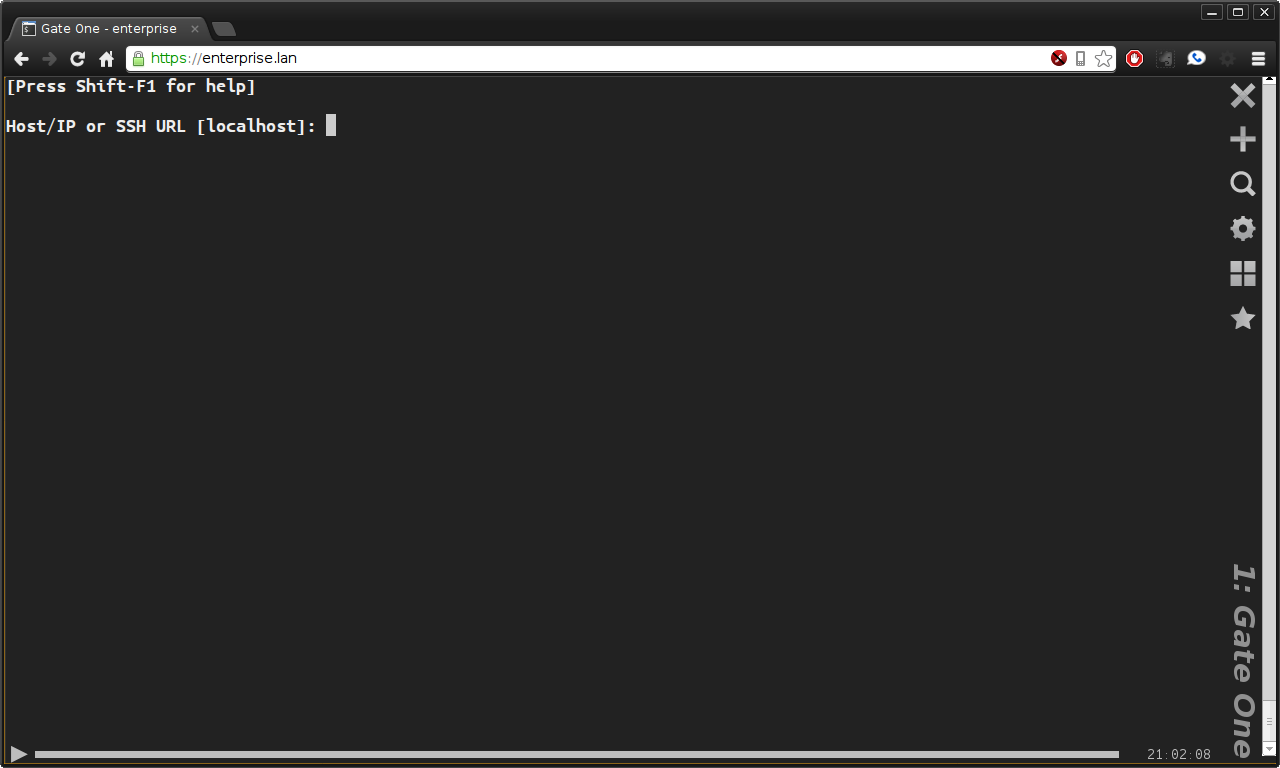
\includegraphics{gateone_login.png}
\caption{The default login screen with the SSH plugin enabled.}\end{figure}

\begin{notice}{note}{Note:}
The text zoom level was increased for all of these screenshots to make them easier to read.
\end{notice}


\paragraph{Detailed Interface Overview}
\label{Applications/terminal/userguide:detailed-interface-overview}
Here's an overview of what each GUI element does:
\begin{figure}[htbp]
\centering
\capstart

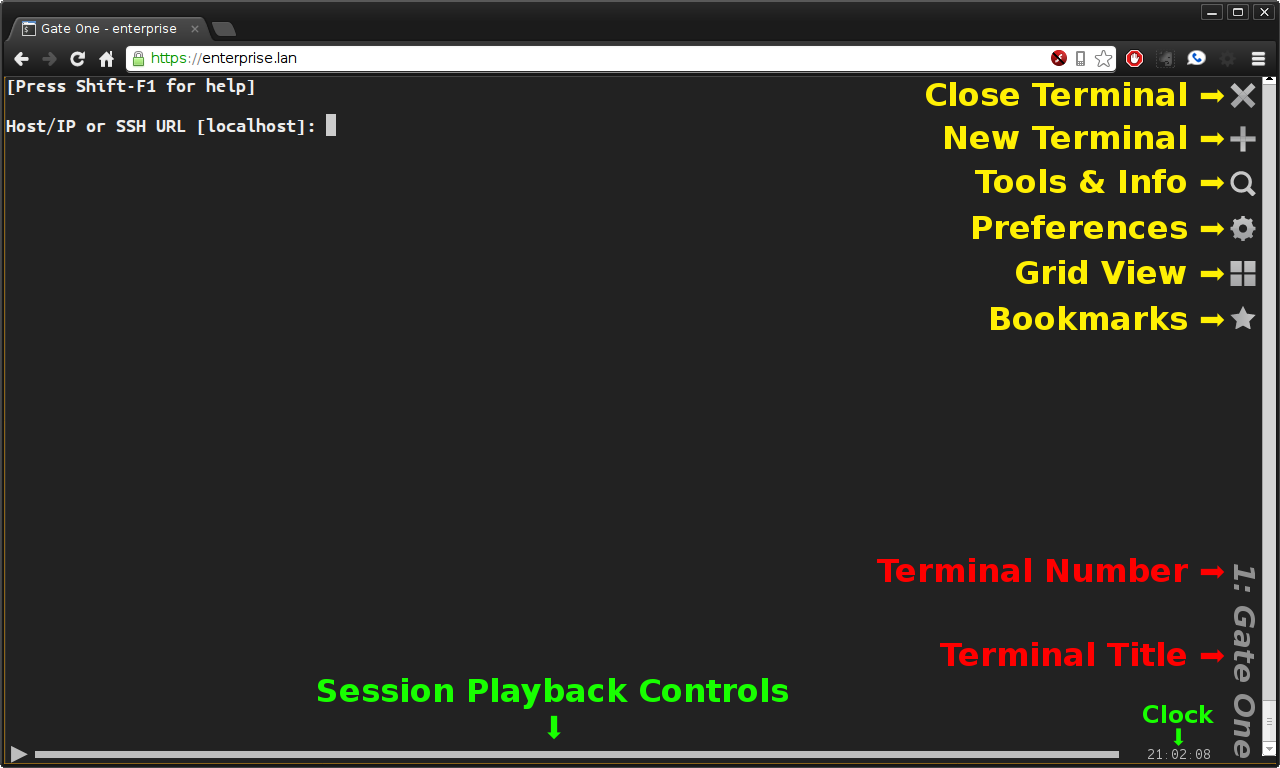
\includegraphics{gateone_login_explained.png}
\caption{Gate One's interface, explained}\end{figure}


\paragraph{Keyboard Shortcuts}
\label{Applications/terminal/userguide:keyboard-shortcuts}
\begin{tabulary}{\linewidth}{|L|L|}
\hline
\textsf{\relax 
Function
} & \textsf{\relax 
Shortcut
}\\
\hline
View The Help
 & 
\code{Shift-F1}
\\
\hline
Open Terminal
 & 
\code{Control-Alt-N}
\\
\hline
Close Terminal
 & 
\code{Control-Alt-W}
\\
\hline
Show Grid
 & 
\code{Control-Alt-G}
\\
\hline
Switch to the terminal on the left
 & 
\code{Shift-LeftArrow}
\\
\hline
Switch to the terminal on the right
 & 
\code{Shift-RightArrow}
\\
\hline
Switch to the terminal above
 & 
\code{Shift-UpArrow}
\\
\hline
Switch to the terminal below
 & 
\code{Shift-DownArrow}
\\
\hline\end{tabulary}



\paragraph{The Toolbar}
\label{Applications/terminal/userguide:the-toolbar}
Gate One's toolbar consists of a number of icons at the right of the window.  These icons are the main source of interaction with Gate One.  It should also be noted that all of Gate One's icons are inline SVG graphics...  So they will scale with your font size and will change color based on your CSS theme.  Another nice feature of the toolbar is that it's trivial for plugins to add their own icons.

\begin{notice}{note}{Note:}
Why are the icons and title on the right and not the top?  Because these days monitors are much wider than they are tall.  In other words, vertical screen space is at a premium while there's plenty of room on the sides.
\end{notice}


\subparagraph{Close Terminal and New Terminal}
\label{Applications/terminal/userguide:close-terminal-and-new-terminal}
These icons do precisely what you'd expect from a modern GUI:  The X icon closes the terminal in the current view while the + icon opens a new terminal.

\begin{notice}{note}{Note:}
If you close the last open terminal a new one will be opened.
\end{notice}


\subparagraph{Terminal Info and Tools}
\label{Applications/terminal/userguide:terminal-info-and-tools}\begin{figure}[htbp]
\centering
\capstart

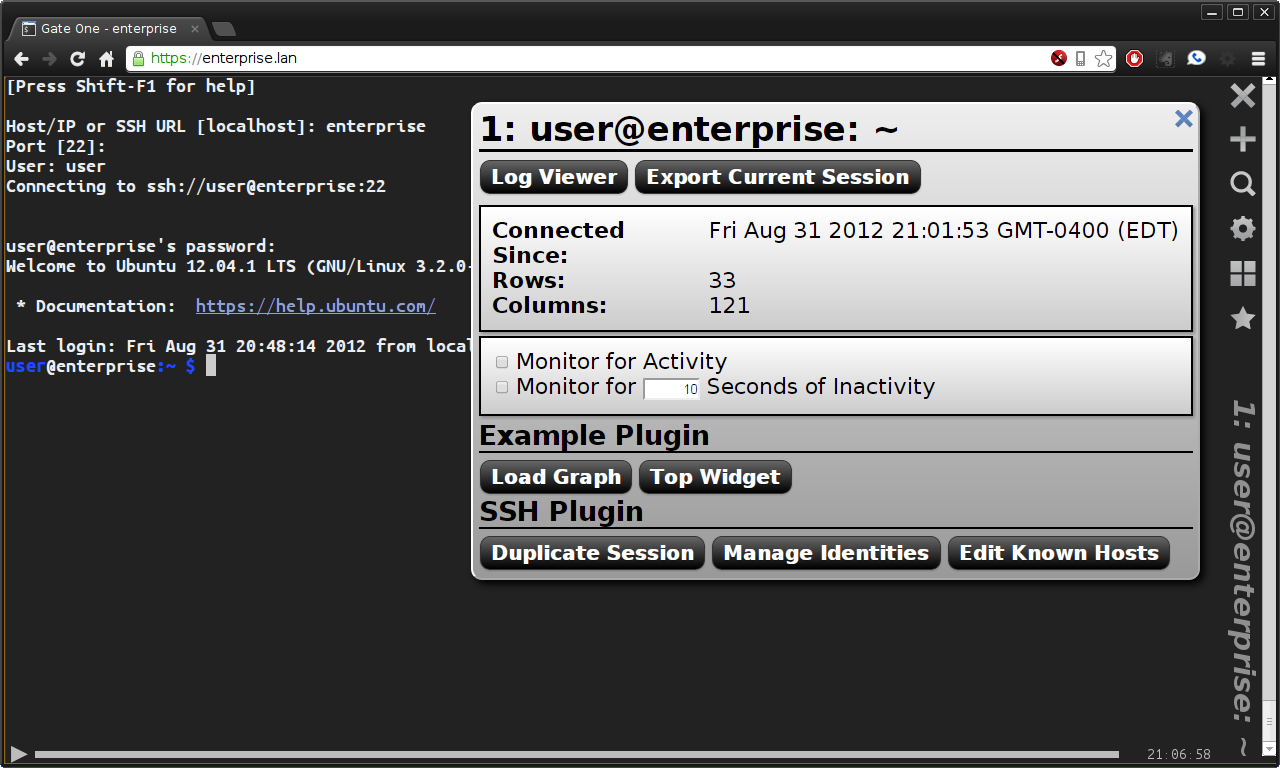
\includegraphics{gateone_infopanel.png}
\caption{This is what you see when you click on the magnifying glass icon}\end{figure}

Gate One's information panel is the place to get information about the current terminal.  By default, it will display the current terminal title, how long the terminal has been open, and the number of rows and columns.  It also presents some options to the user which are outlined below...

\begin{notice}{tip}{Tip:}
You can manually change the current terminal title by clicking on it.
\end{notice}


\subparagraph{Log Viewer}
\label{Applications/terminal/userguide:log-viewer}
Gate One's log viewer provides a mechanism for viewing the logs of terminal sessions stored on the server.  Log metadata as well as a preview can be viewed by simply clicking on any given log.  Playback and flat (traditional) viewing options are also available.  These will open in a new window.
\begin{figure}[htbp]
\centering
\capstart

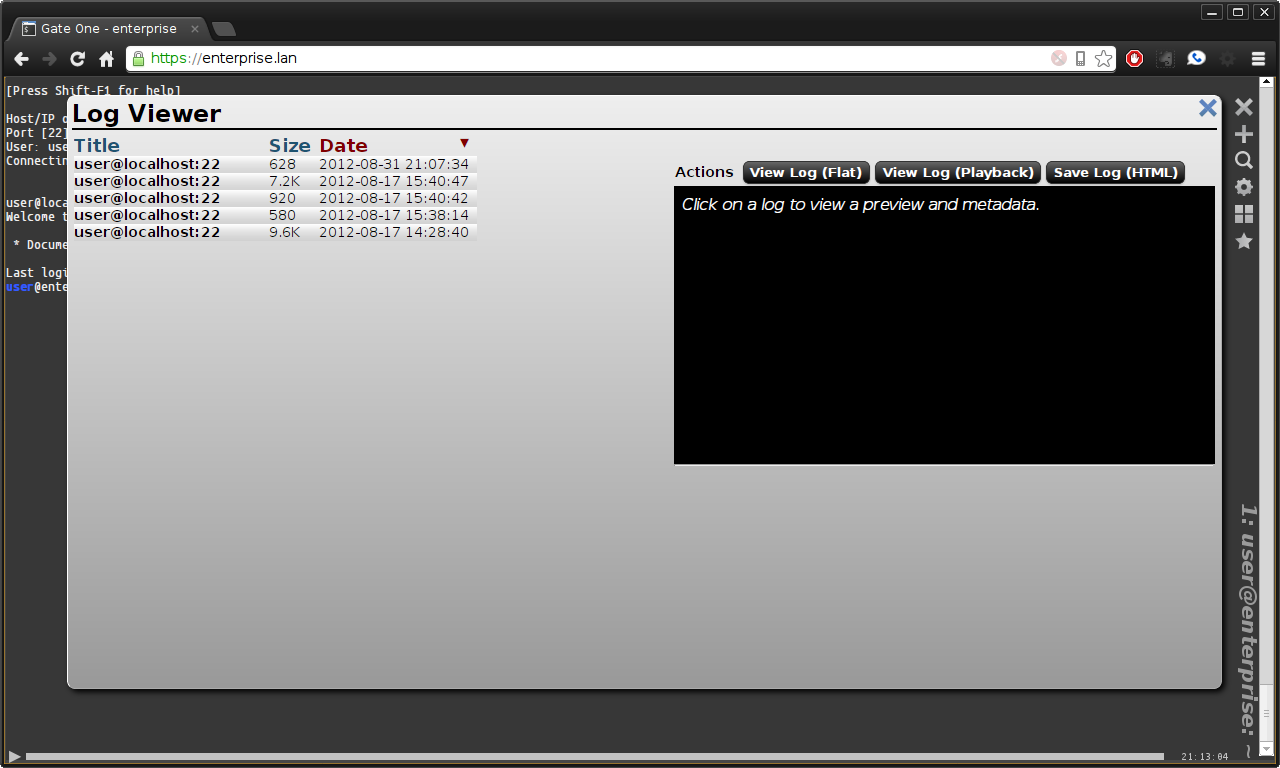
\includegraphics{gateone_log_viewer.png}
\caption{Gate One's Log Viewer (unzoomed)}\end{figure}

\begin{notice}{tip}{Tip:}
When you open the log viewer it will display a message indicating how many logs there are associated with your user account along with the total amount of space the logs are taking up on the server.
\end{notice}

\begin{notice}{note}{Note:}
Gate One's log format is pre-compressed using gzip.  There's no need to compress them.
\end{notice}


\subparagraph{Export Current Session}
\label{Applications/terminal/userguide:export-current-session}
When this button is clicked it will open up a new browser tab that will play back the current terminal's session.  This recording is self-contained and can be saved to your computer for playback later.  Everything needed to play back the recording is contained within the HTML file itself.  You can share it with friends, plop it into an iframe on a website, or just email it to someone.  It will even auto-scale itself (down) if necessary to fit within the current frame or window.

\begin{notice}{note}{Note:}
This kind of session recording is merely a shortcut to quickly exporting the current terminal session.  You can always access your server-side session logs from within the log viewer.
\end{notice}


\subparagraph{Monitor for Activity/Inactivity}
\label{Applications/terminal/userguide:monitor-for-activity-inactivity}
This feature allows you to monitor the current terminal for either activity (e.g. something changes) or inactivity (e.g. when the terminal stops changing).  When either of these events is triggered Gate One will play a sound and pop up an alert to notify you which terminal has passed the threshold for activity or inactivity.

\begin{notice}{tip}{Tip:}
This feature is very handy for when you want to know when, say, a download is complete (inactivity: ``wget \textless{}url\textgreater{}'' finishes) or when someone hits your website (activity: a ``tail -f'' on the log suddenly has output).
\end{notice}


\subparagraph{SSH Plugin: Duplicate Session}
\label{Applications/terminal/userguide:ssh-plugin-duplicate-session}
You'll see this option if the SSH plugin is enabled...  This button allows you to duplicate your current SSH session.  It will open a new SSH connection to the current server using the exact same SSH connect string (e.g. ssh://user@host:22) that was used to connect originally.  Also, if possible, it will utilize the existing SSH tunnel for this connection which means you won't have to re-enter your password.  When this (awesome) feature is invoked you'll see a message indicating as such in the terminal:
\begin{figure}[htbp]
\centering
\capstart

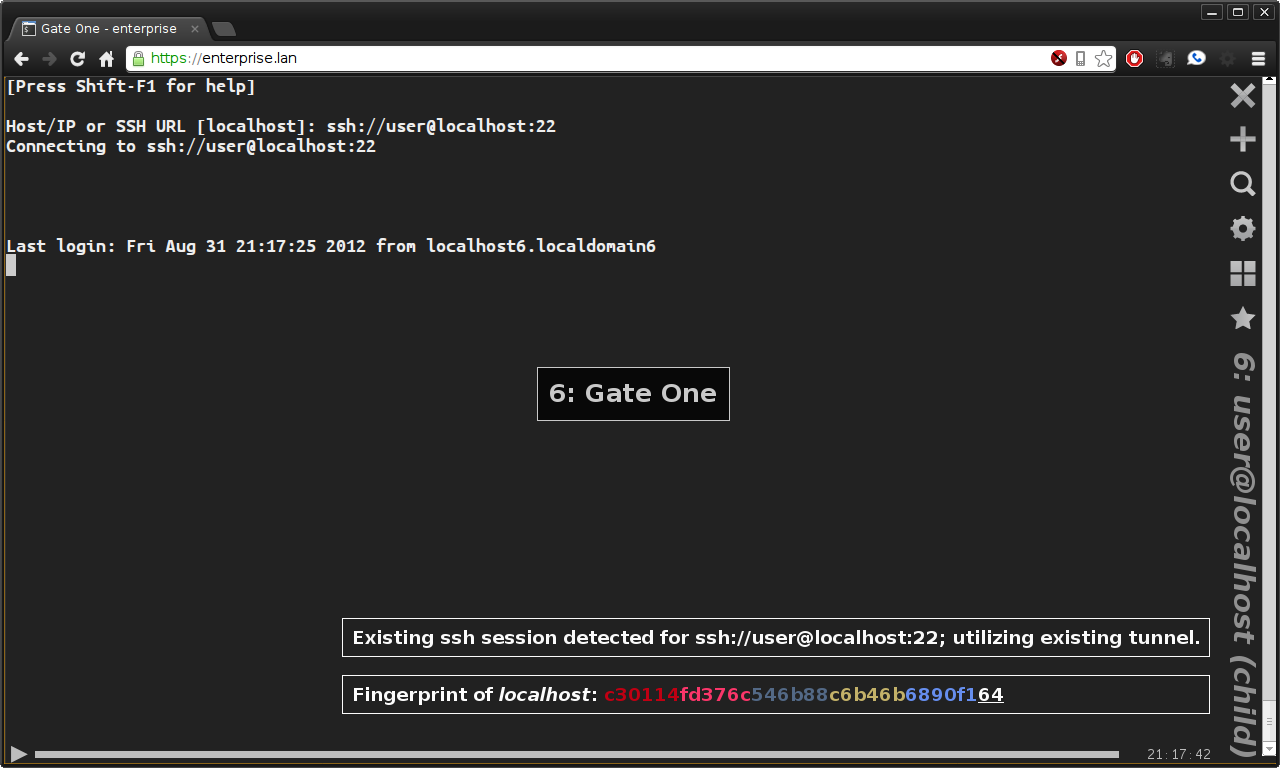
\includegraphics{gateone_second_session_no_password.png}
\caption{After duplicating an SSH session.  No password required!}\end{figure}


\subparagraph{SSH Plugin: Manage Identities}
\label{Applications/terminal/userguide:ssh-plugin-manage-identities}
The SSH plugin includes an interface for managing all of your SSH identities (aka SSH keys).  Here, SSH identities (private and public key files) can be generated, downloaded, uploaded, or deleted.  There is also support for uploading (or replacing existing) X.509 certificates that may be associated with a given identity.  X.509 support is important because it provides the ability for keys to be revoked (e.g. in the event that an employee leaves your company).  X.509 certificates can also restrict what privileges a user has when logging into a server via SSH (e.g. disallowing port forwarding).  If any of these restrictions are present in a given Identity's X.509 certificate they will be displayed in place of the randomart field.
\begin{figure}[htbp]
\centering
\capstart

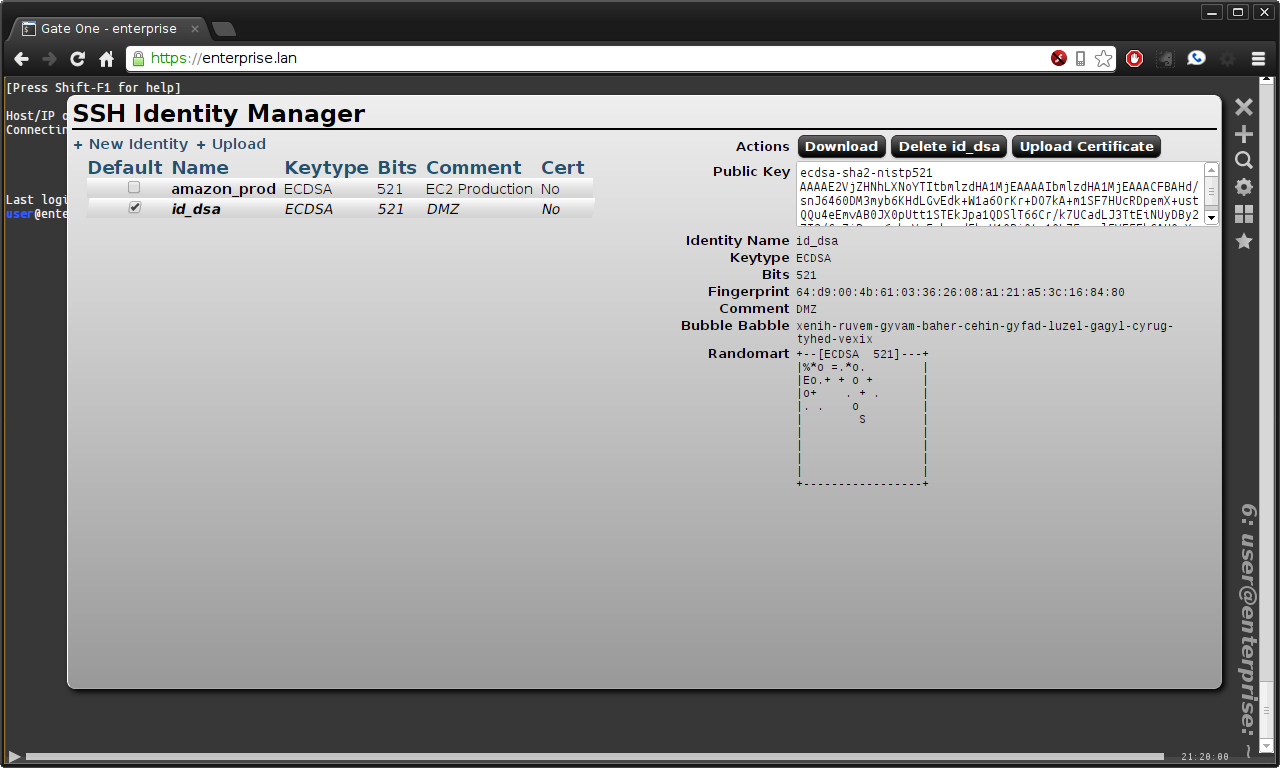
\includegraphics{gateone_ssh_identity_manager.png}
\caption{SSH Identity Manager (unzoomed)}\end{figure}

\begin{notice}{tip}{Tip:}
If you hover your mouse over the title of each column it will provide detailed description of what it means.
\end{notice}
\paragraph{The SSH Identity Manager also allows you to generate new identities...}
\begin{figure}[htbp]
\centering
\capstart

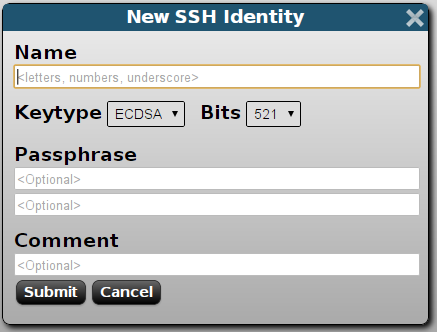
\includegraphics{gateone_new_ssh_identity.png}
\caption{Generate New Identity}\end{figure}
\paragraph{Upload existing identities...}

\begin{notice}{tip}{Tip:}
If you upload a private key without a public key Gate One will automatically derive the public key from the private one.  Super handy for Amazon EC2 SSH identities where they don't give you the public key.
\end{notice}
\begin{figure}[htbp]
\centering
\capstart

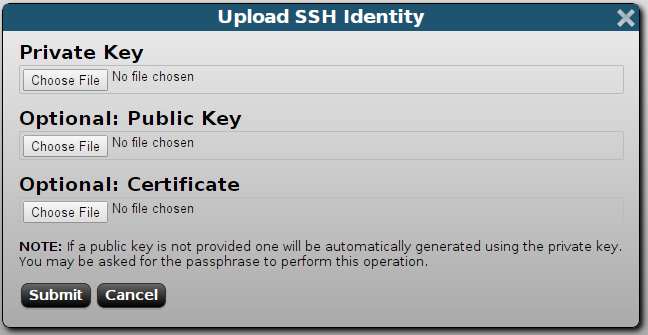
\includegraphics{gateone_upload_ssh_identity.png}
\caption{Upload Identity}\end{figure}
\paragraph{And upload X.509 certificates...}
\begin{figure}[htbp]
\centering
\capstart

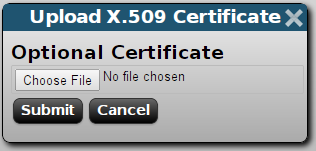
\includegraphics{gateone_upload_x509.png}
\caption{Upload X.509 Certificate}\end{figure}


\subparagraph{Edit Known Hosts}
\label{Applications/terminal/userguide:edit-known-hosts}
Clicking this button will bring up an editor for Gate One's equivalent of \textasciitilde{}/.ssh/known\_hosts (same file, different location).  This will be handy if some server you connect to on a regular basis ever changes its host key...  You'll need to delete the corresponding line.

\begin{notice}{note}{Note:}
Line numbers in the textarea are forthcoming (to make finding the appropriate host line easier).
\end{notice}


\subparagraph{The Settings Panel}
\label{Applications/terminal/userguide:the-settings-panel}\begin{figure}[htbp]
\centering
\capstart

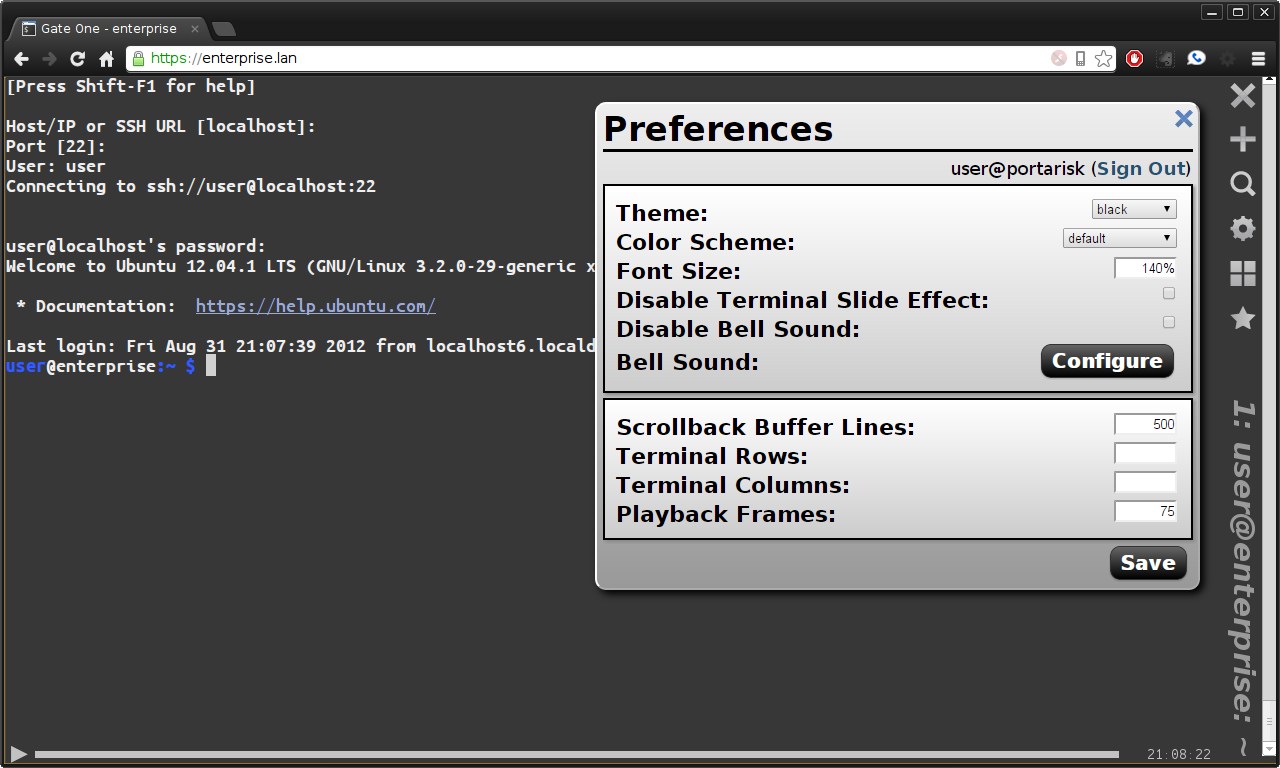
\includegraphics{gateone_settingspanel.png}
\caption{Gate One's Settings Panel}\end{figure}

These options are detailed below...


\subparagraph{Theme}
\label{Applications/terminal/userguide:theme}
This controls the look and feel of Gate One.  When selected, the chosen theme will take effect right away.
\begin{figure}[htbp]
\centering
\capstart

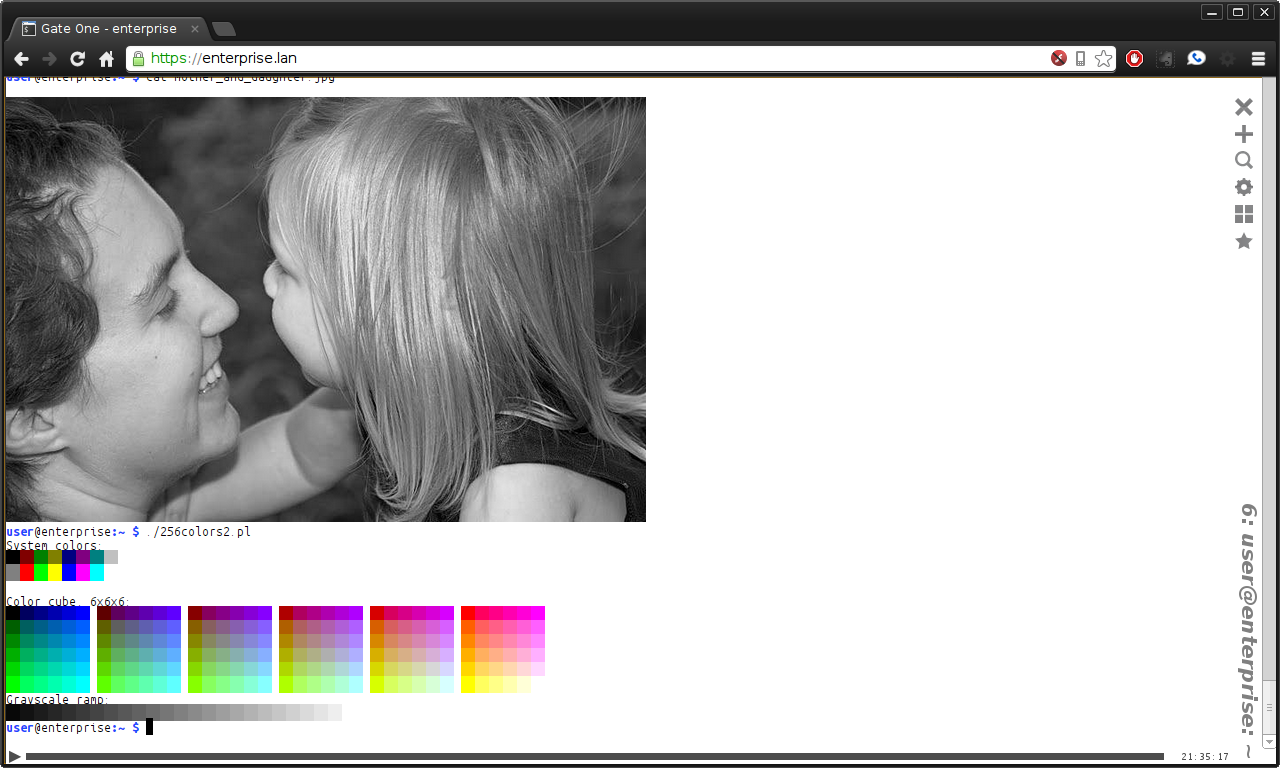
\includegraphics{gateone_white_theme.png}
\caption{White Theme}\end{figure}

\begin{notice}{tip}{Tip:}
Themes are just CSS files and are easy to edit.  \code{black.css} and \code{white.css} are in \code{\textless{}path to gateone\textgreater{}/templates/themes}.  Copy one and start making your own!  If it turns out pretty good send it to us and we'll include it with Gate One.
\end{notice}

\begin{notice}{note}{Note:}
The black scheme doesn't actually have a black background (it's \#222)...  Why?  So the panels can have shadows which provides important contrast.  Essentially, it is easier on the eyes.
\end{notice}


\subparagraph{Color Scheme}
\label{Applications/terminal/userguide:color-scheme}
This is similar to the ``Theme'' option above but it only controls the colors of terminal text (aka renditions).

\begin{notice}{note}{Note:}
CSS color schemes can be found in \code{\textless{}path to gateone\textgreater{}/templates/term\_colors}.
\end{notice}


\subparagraph{Scrollback Buffer Lines}
\label{Applications/terminal/userguide:scrollback-buffer-lines}
This option tells Gate One how many lines to keep in the scrollback buffer (in memory).  When you're typing or when a terminal is updating itself Gate One only updates the browser window with what falls within the terminal's rows and columns.  Only after a timeout of 3.5 seconds does it re-attach the scrollback buffer.  When this happens the browser has to render all that text; the more there is the longer it takes (milliseconds).  Even on a slow system 500 lines (the default) should be unnoticably speedy.

\begin{notice}{tip}{Tip:}
You don't have to wait for the 3.5 second timeout:  Just start scrolling and the timeout will be cancelled and the scrollback buffer will be immediately prepended to the current view.
\end{notice}

\begin{notice}{note}{Note:}
Why the complexity?  The more text that is being rendered, the slower the browser will be able to update your terminal window.  If we updated the current number of rows + the number of lines in the scrollback buffer every time you pressed a key this would quickly bog down your browser and make Gate One considerably less responsive.
\end{notice}


\subparagraph{Playback Frames}
\label{Applications/terminal/userguide:playback-frames}
This option controls how many frames of real-time session playback will be kept in working memory.  The higher the number, the more memory it will use.  Also, the more terminals you have open the higher the memory use as well.  Having said that, 200-500 frames per terminal shouldn't be of any concern for a modern computer.

\begin{notice}{tip}{Tip:}
If you hold down the Shift key while scrolling with your mouse wheel it will move backwards and forwards in the playback buffer instead of scrolling up and down.  It is a handy way to see the history of full-screen applications such as `top'.
\end{notice}


\subparagraph{Terminal Rows and Terminal Columns}
\label{Applications/terminal/userguide:terminal-rows-and-terminal-columns}
By default these are blank which means Gate One will automatically figure out how many rows and columns will fit in a given terminal window.  If you set these, Gate One will force these values on all running terminal programs.  The ability to set this on a per-terminal basis is forthcoming.

\begin{notice}{note}{Note:}
Why would anyone bother?  Some legacy/poorly-written terminal programs only work properly in a terminal window of 24 rows and 80 columns.
\end{notice}


\subparagraph{Gate One's Grid}
\label{Applications/terminal/userguide:gate-one-s-grid}
Gate One lays out terminals in a grid like so:

\begin{tabulary}{\linewidth}{|L|L|}
\hline

Terminal 1
 & 
Terminal 2
\\
\hline
Terminal 3
 & 
Terminal 4
\\
\hline
Terminal 5
 & 
Terminal 6
\\
\hline
So on
 & 
And so on
\\
\hline\end{tabulary}


The grid view can be invoked by either clicking on the Grid icon (four squares) in the toolbar or via the Ctrl-Alt-G keyboard shortcut.  Here's what it looks like:
\begin{figure}[htbp]
\centering
\capstart

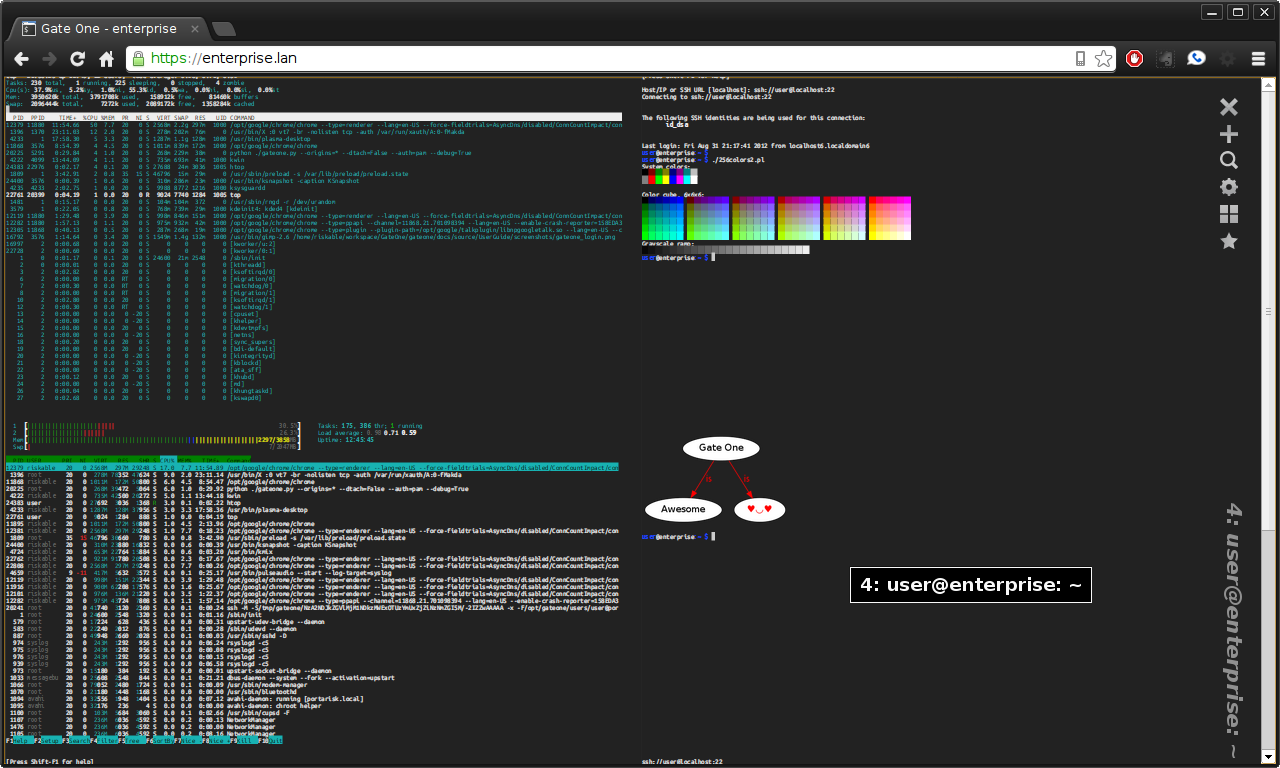
\includegraphics{gateone_grid_view.png}
\caption{The Grid View.  The mouse was moved over Terminal 4 in this example, demonstrating the mouseover effect.}\end{figure}


\subparagraph{The Bookmark Manager}
\label{Applications/terminal/userguide:the-bookmark-manager}
The first time you open the Bookmarks manager it will be empty:
\begin{figure}[htbp]
\centering
\capstart

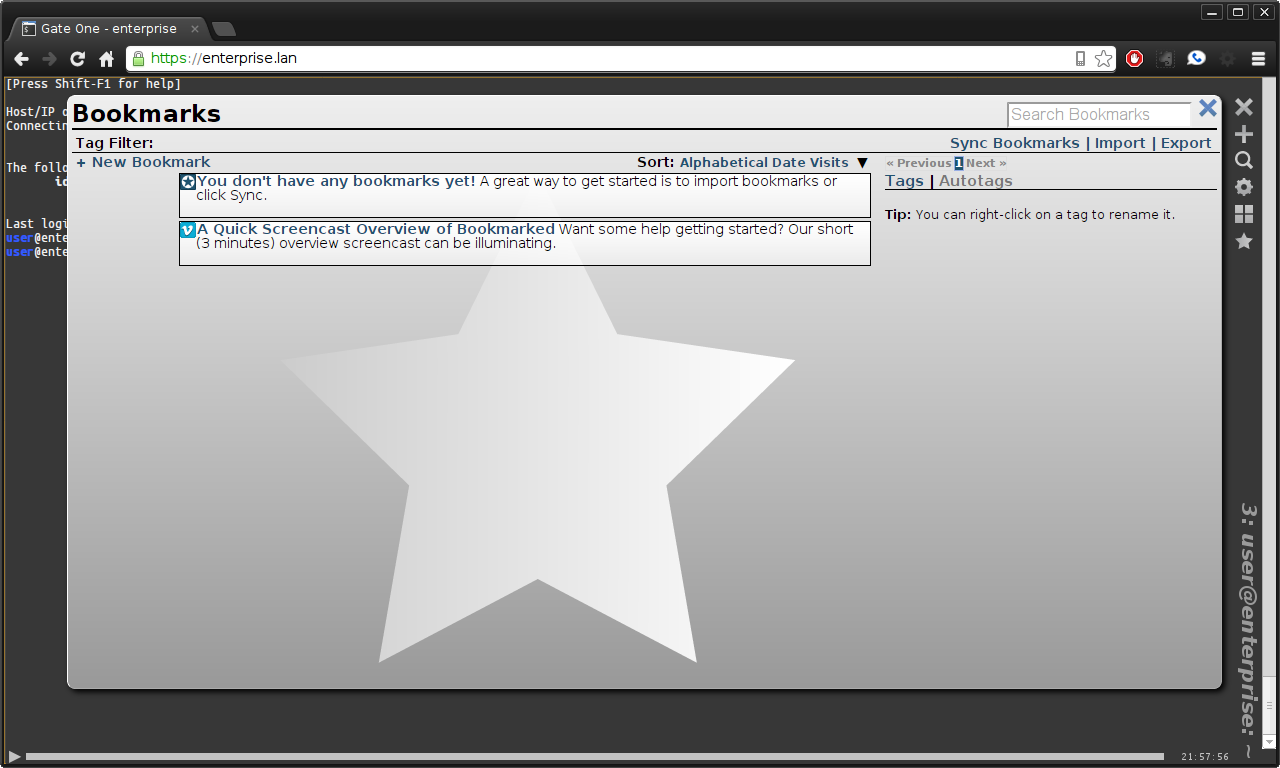
\includegraphics{gateone_bookmarks_empty.png}
\caption{No bookmarks yet!}\end{figure}

Bookmarks can be added by clicking on ``New'':
\begin{figure}[htbp]
\centering
\capstart

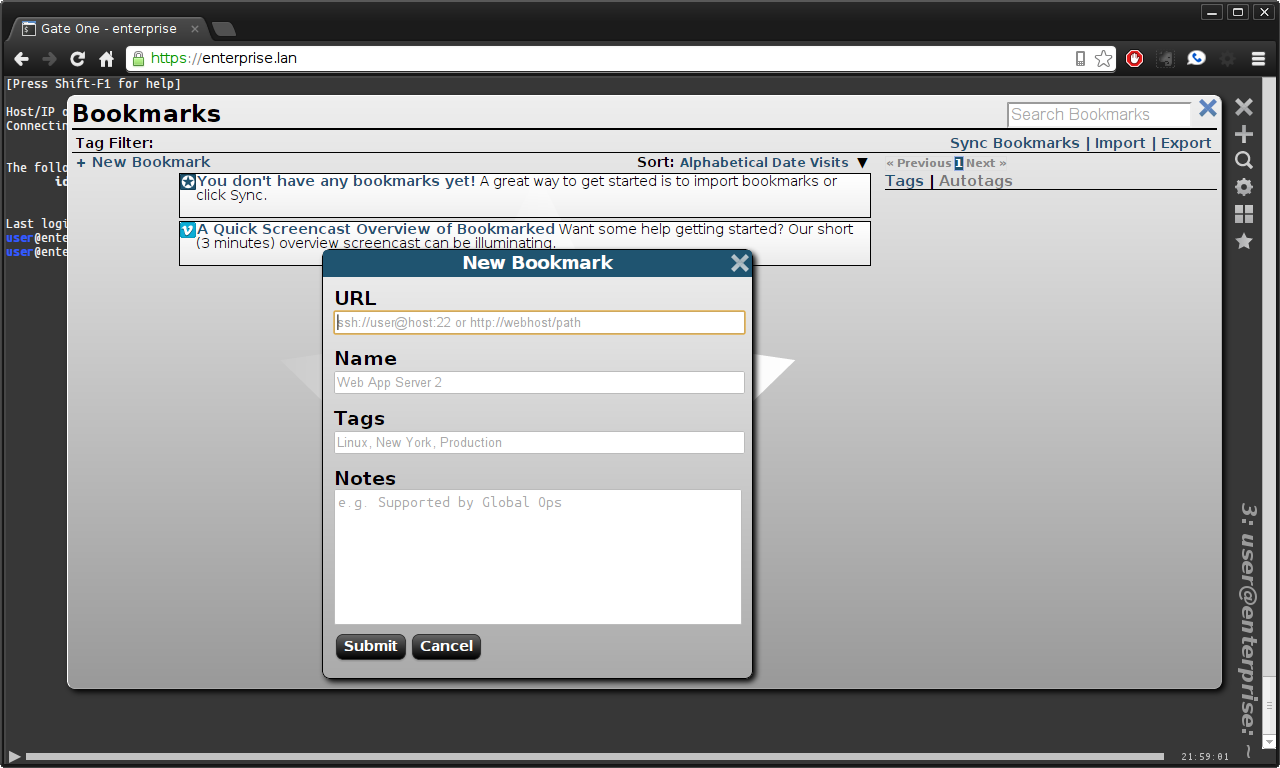
\includegraphics{gateone_new_bookmark1.png}
\caption{The New Bookmark Form.}\end{figure}

Here's an example of the new bookmark form, filled out with a new SSH bookmark:
\begin{figure}[htbp]
\centering
\capstart

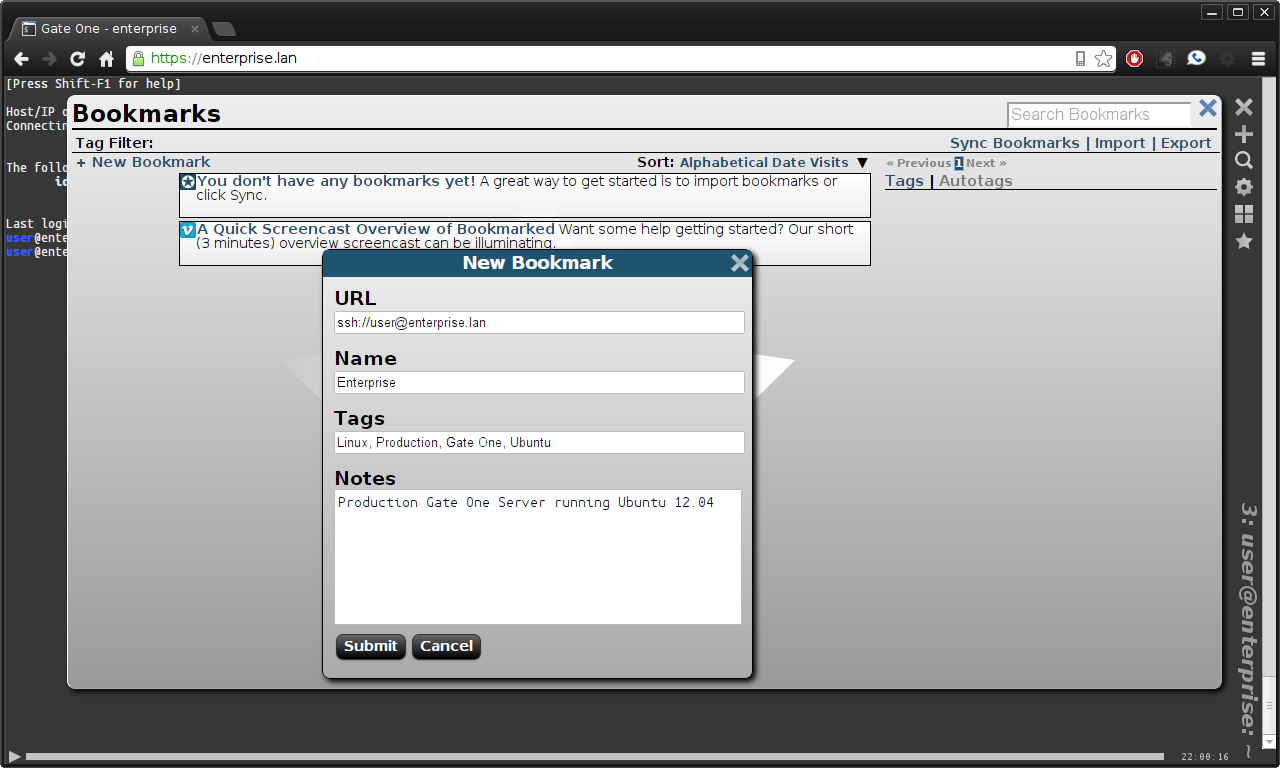
\includegraphics{gateone_new_bookmark2.png}
\caption{SSH Bookmark to the Gate One Demo Server}\end{figure}

After submitting the form (which doesn't actually submit anything to the Gate One server) we can see our first bookmark in the panel:
\begin{figure}[htbp]
\centering
\capstart

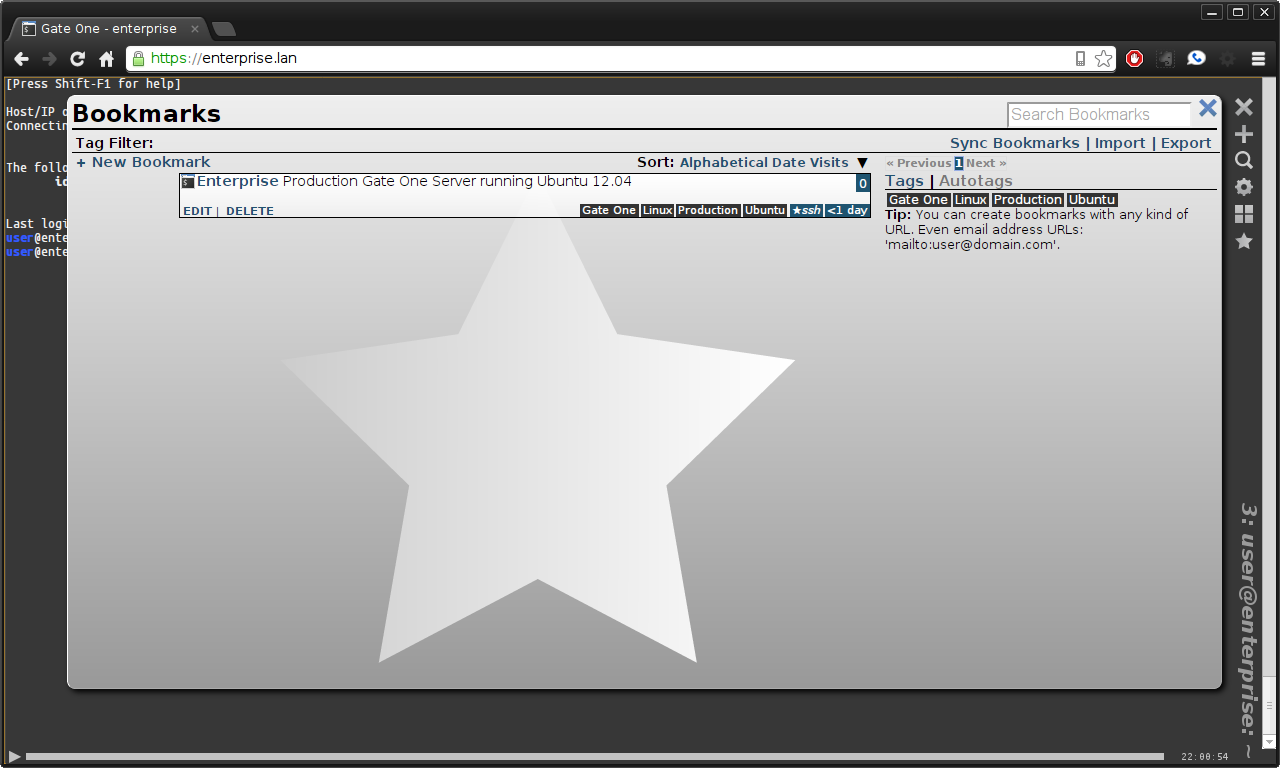
\includegraphics{gateone_new_bookmark3.png}
\caption{Finally, a bookmark!}\end{figure}

Here's what the panel will look like after you've added a number of bookmarks:
\begin{figure}[htbp]
\centering
\capstart

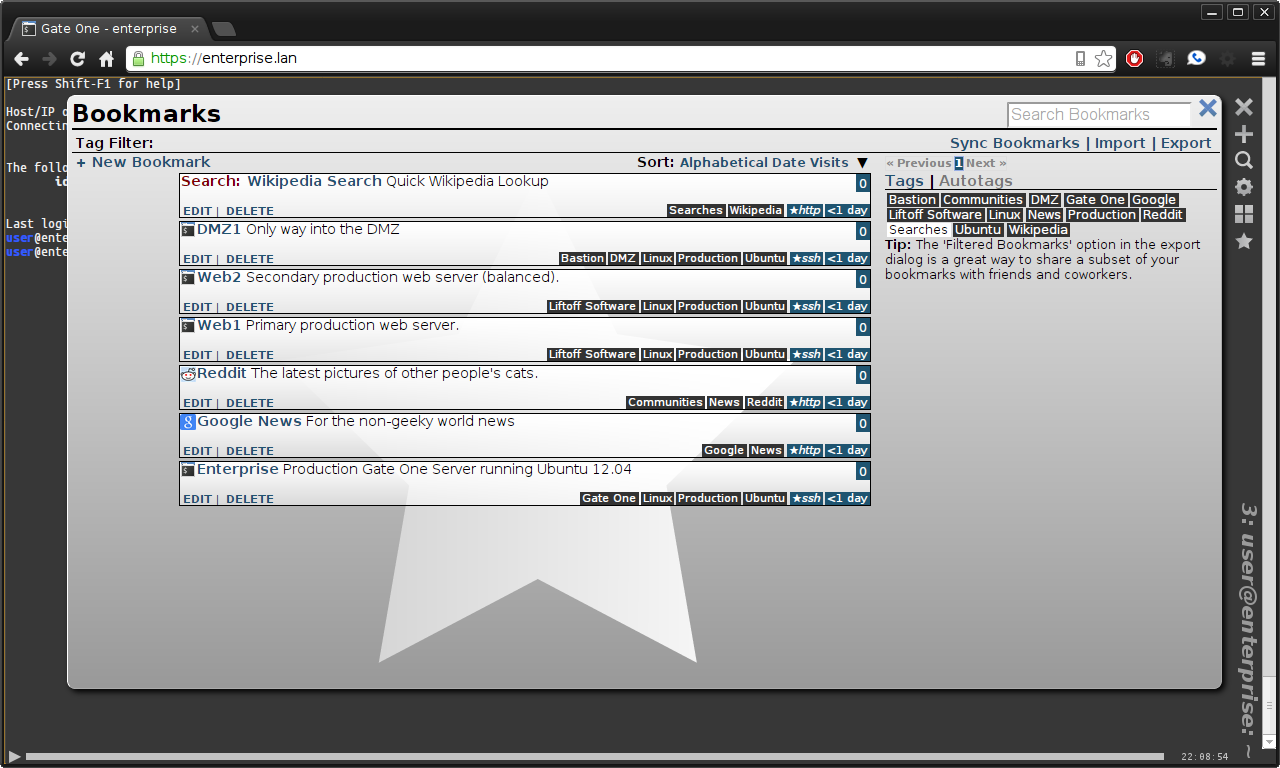
\includegraphics{gateone_new_bookmark4.png}
\caption{In this example we have both SSH bookmarks and an HTTP bookmark.}\end{figure}

\begin{notice}{tip}{Tip:}
Clicking on any of those tags will filter the current view to only show bookmarks that have been tagged as such.
\end{notice}

Lastly, here's what happens when you click on an SSH bookmark:
\begin{figure}[htbp]
\centering
\capstart

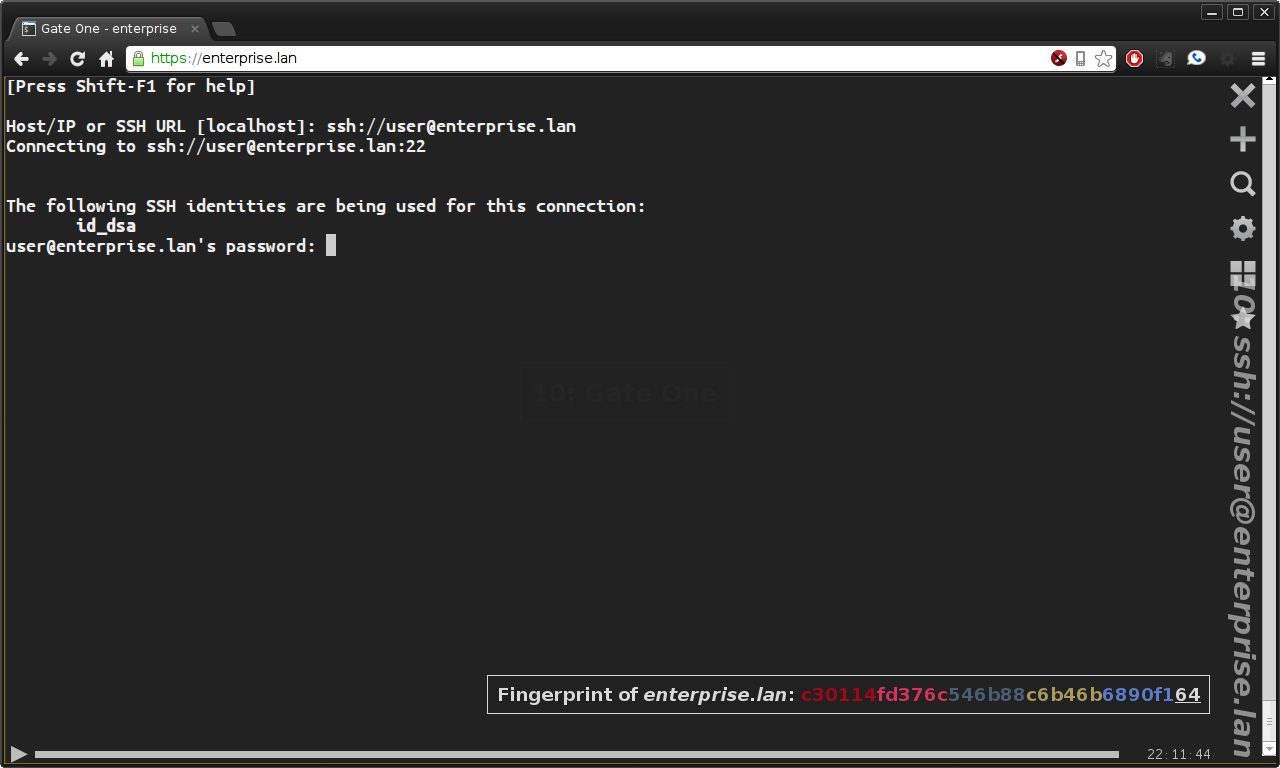
\includegraphics{gateone_opened_via_bookmark.png}
\caption{This bookmark was automatically opened in a new terminal.}\end{figure}

In the example above, the ssh:// URL was automatically entered for us.  All we had to do was enter our password.


\subsubsection{Terminal Developer Documentation}
\label{Applications/terminal/developer:terminal-developer-documentation}\label{Applications/terminal/developer::doc}

\paragraph{Python Code}
\label{Applications/terminal/developer:python-code}

\subparagraph{\texttt{app\_terminal.py} - Gate One Terminal Application}
\label{Applications/terminal/app_terminal:module-app_terminal}\label{Applications/terminal/app_terminal::doc}\label{Applications/terminal/app_terminal:app-terminal-py-gate-one-terminal-application}\index{app\_terminal (module)}
A Gate One Application (\code{GOApplication}) that provides a terminal emulator.
\index{kill\_session() (in module app\_terminal)}

\begin{fulllineitems}
\phantomsection\label{Applications/terminal/app_terminal:app_terminal.kill_session}\pysiglinewithargsret{\code{app\_terminal.}\bfcode{kill\_session}}{\emph{session}, \emph{kill\_dtach=False}}{}
Terminates all the terminal processes associated with \emph{session}.  If
\emph{kill\_dtach} is True, the dtach processes associated with the session will
also be killed.

\begin{notice}{note}{Note:}
This function gets appended to the
\code{SESSIONS{[}session{]}{[}"kill\_session\_callbacks"{]}} list inside of
{\hyperref[Applications/terminal/app_terminal:app_terminal.TerminalApplication.authenticate]{\code{TerminalApplication.authenticate()}}}.
\end{notice}

\end{fulllineitems}

\index{timeout\_session() (in module app\_terminal)}

\begin{fulllineitems}
\phantomsection\label{Applications/terminal/app_terminal:app_terminal.timeout_session}\pysiglinewithargsret{\code{app\_terminal.}\bfcode{timeout\_session}}{\emph{session}}{}
Attached to Gate One's `timeout\_callbacks'; kills the given session.

If `dtach' support is enabled the dtach processes associated with the
session will also be killed.

\end{fulllineitems}

\index{SharedTermHandler (class in app\_terminal)}

\begin{fulllineitems}
\phantomsection\label{Applications/terminal/app_terminal:app_terminal.SharedTermHandler}\pysiglinewithargsret{\strong{class }\code{app\_terminal.}\bfcode{SharedTermHandler}}{\emph{application}, \emph{request}, \emph{**kwargs}}{}
Renders shared.html which allows an anonymous user to view a shared
terminal.

\end{fulllineitems}

\index{TermStaticFiles (class in app\_terminal)}

\begin{fulllineitems}
\phantomsection\label{Applications/terminal/app_terminal:app_terminal.TermStaticFiles}\pysiglinewithargsret{\strong{class }\code{app\_terminal.}\bfcode{TermStaticFiles}}{\emph{application}, \emph{request}, \emph{**kwargs}}{}
Serves static files in the \code{gateone/applications/terminal/static} directory.

\begin{notice}{note}{Note:}
This is configured via the \code{web\_handlers} global (a feature inherent to
Gate One applications).
\end{notice}

\end{fulllineitems}

\index{TerminalApplication (class in app\_terminal)}

\begin{fulllineitems}
\phantomsection\label{Applications/terminal/app_terminal:app_terminal.TerminalApplication}\pysiglinewithargsret{\strong{class }\code{app\_terminal.}\bfcode{TerminalApplication}}{\emph{ws}}{}
A Gate One Application (\code{GOApplication}) that handles creating and
controlling terminal applications running on the Gate One server.
\index{initialize() (app\_terminal.TerminalApplication method)}

\begin{fulllineitems}
\phantomsection\label{Applications/terminal/app_terminal:app_terminal.TerminalApplication.initialize}\pysiglinewithargsret{\bfcode{initialize}}{}{}
Called when the WebSocket is instantiated, sets up our WebSocket
actions, security policies, and attaches all of our plugin hooks/events.

\end{fulllineitems}

\index{open() (app\_terminal.TerminalApplication method)}

\begin{fulllineitems}
\phantomsection\label{Applications/terminal/app_terminal:app_terminal.TerminalApplication.open}\pysiglinewithargsret{\bfcode{open}}{}{}
This gets called at the end of \code{ApplicationWebSocket.open()} when
the WebSocket is opened.

\end{fulllineitems}

\index{send\_client\_files() (app\_terminal.TerminalApplication method)}

\begin{fulllineitems}
\phantomsection\label{Applications/terminal/app_terminal:app_terminal.TerminalApplication.send_client_files}\pysiglinewithargsret{\bfcode{send\_client\_files}}{}{}
Sends the client our standard CSS and JS.

\end{fulllineitems}

\index{authenticate() (app\_terminal.TerminalApplication method)}

\begin{fulllineitems}
\phantomsection\label{Applications/terminal/app_terminal:app_terminal.TerminalApplication.authenticate}\pysiglinewithargsret{\bfcode{authenticate}}{}{}
This gets called immediately after the user is authenticated
successfully at the end of \code{ApplicationWebSocket.authenticate()}.
Sends all plugin JavaScript files to the client and triggers the
`terminal:authenticate' event.

\end{fulllineitems}

\index{on\_close() (app\_terminal.TerminalApplication method)}

\begin{fulllineitems}
\phantomsection\label{Applications/terminal/app_terminal:app_terminal.TerminalApplication.on_close}\pysiglinewithargsret{\bfcode{on\_close}}{}{}
Removes all attached callbacks and triggers the \code{terminal:on\_close}
event.

\end{fulllineitems}

\index{enumerate\_fonts() (app\_terminal.TerminalApplication method)}

\begin{fulllineitems}
\phantomsection\label{Applications/terminal/app_terminal:app_terminal.TerminalApplication.enumerate_fonts}\pysiglinewithargsret{\bfcode{enumerate\_fonts}}{}{}
Returns a JSON-encoded object containing the installed fonts.

\end{fulllineitems}

\index{enumerate\_colors() (app\_terminal.TerminalApplication method)}

\begin{fulllineitems}
\phantomsection\label{Applications/terminal/app_terminal:app_terminal.TerminalApplication.enumerate_colors}\pysiglinewithargsret{\bfcode{enumerate\_colors}}{}{}
Returns a JSON-encoded object containing the installed text color
schemes.

\end{fulllineitems}

\index{save\_term\_settings() (app\_terminal.TerminalApplication method)}

\begin{fulllineitems}
\phantomsection\label{Applications/terminal/app_terminal:app_terminal.TerminalApplication.save_term_settings}\pysiglinewithargsret{\bfcode{save\_term\_settings}}{\emph{term}, \emph{settings}}{}
Saves whatever \emph{settings} (must be JSON-encodable) are provided in the
user's session directory; associated with the given \emph{term}.

The {\hyperref[Applications/terminal/app_terminal:app_terminal.TerminalApplication.restore_term_settings]{\code{restore\_term\_settings}}} function can be used to restore the provided
settings.

\begin{notice}{note}{Note:}
This method is primarily to aid dtach support.
\end{notice}

\end{fulllineitems}

\index{restore\_term\_settings() (app\_terminal.TerminalApplication method)}

\begin{fulllineitems}
\phantomsection\label{Applications/terminal/app_terminal:app_terminal.TerminalApplication.restore_term_settings}\pysiglinewithargsret{\bfcode{restore\_term\_settings}}{\emph{term}}{}
Reads the settings associated with the given \emph{term} that are stored in
the user's session directory and applies them to
\code{self.loc\_terms{[}term{]}}

\end{fulllineitems}

\index{clear\_term\_settings() (app\_terminal.TerminalApplication method)}

\begin{fulllineitems}
\phantomsection\label{Applications/terminal/app_terminal:app_terminal.TerminalApplication.clear_term_settings}\pysiglinewithargsret{\bfcode{clear\_term\_settings}}{\emph{term}}{}
Removes any settings associated with the given \emph{term} in the user's
term\_settings.json file (in their session directory).

\end{fulllineitems}

\index{term\_ended() (app\_terminal.TerminalApplication method)}

\begin{fulllineitems}
\phantomsection\label{Applications/terminal/app_terminal:app_terminal.TerminalApplication.term_ended}\pysiglinewithargsret{\bfcode{term\_ended}}{\emph{term}}{}
Sends the `term\_ended' message to the client letting it know that the
given \emph{term} is no more.

\end{fulllineitems}

\index{add\_terminal\_callbacks() (app\_terminal.TerminalApplication method)}

\begin{fulllineitems}
\phantomsection\label{Applications/terminal/app_terminal:app_terminal.TerminalApplication.add_terminal_callbacks}\pysiglinewithargsret{\bfcode{add\_terminal\_callbacks}}{\emph{term}, \emph{multiplex}, \emph{callback\_id}}{}
Sets up all the callbacks associated with the given \emph{term}, \emph{multiplex}
instance and \emph{callback\_id}.

\end{fulllineitems}

\index{remove\_terminal\_callbacks() (app\_terminal.TerminalApplication method)}

\begin{fulllineitems}
\phantomsection\label{Applications/terminal/app_terminal:app_terminal.TerminalApplication.remove_terminal_callbacks}\pysiglinewithargsret{\bfcode{remove\_terminal\_callbacks}}{\emph{multiplex}, \emph{callback\_id}}{}
Removes all the Multiplex and terminal emulator callbacks attached to
the given \emph{multiplex} instance and \emph{callback\_id}.

\end{fulllineitems}

\index{new\_multiplex() (app\_terminal.TerminalApplication method)}

\begin{fulllineitems}
\phantomsection\label{Applications/terminal/app_terminal:app_terminal.TerminalApplication.new_multiplex}\pysiglinewithargsret{\bfcode{new\_multiplex}}{\emph{cmd}, \emph{term\_id}, \emph{logging=True}, \emph{encoding=u'utf-8'}, \emph{debug=False}}{}
Returns a new instance of \code{termio.Multiplex} with the proper
global and client-specific settings.
\begin{quote}
\begin{quote}\begin{description}
\item[{cmd}] \leavevmode
The command to execute inside of Multiplex.

\item[{term\_id}] \leavevmode
The terminal to associate with this Multiplex or a descriptive
identifier (it's only used for logging purposes).

\item[{logging}] \leavevmode
If \code{False}, logging will be disabled for this instance of
Multiplex (even if it would otherwise be enabled).

\item[{encoding}] \leavevmode
The default encoding that will be used when reading or writing
to the Multiplex instance.

\item[{debug}] \leavevmode
If \code{True}, will enable debugging on the created Multiplex
instance.

\end{description}\end{quote}
\end{quote}

\end{fulllineitems}

\index{highest\_term\_num() (app\_terminal.TerminalApplication method)}

\begin{fulllineitems}
\phantomsection\label{Applications/terminal/app_terminal:app_terminal.TerminalApplication.highest_term_num}\pysiglinewithargsret{\bfcode{highest\_term\_num}}{\emph{location=None}}{}
Returns the highest terminal number at the given \emph{location} (so we can
figure out what's next).  If \emph{location} is omitted, uses
\code{self.ws.location}.

\end{fulllineitems}

\index{send\_term\_encoding() (app\_terminal.TerminalApplication method)}

\begin{fulllineitems}
\phantomsection\label{Applications/terminal/app_terminal:app_terminal.TerminalApplication.send_term_encoding}\pysiglinewithargsret{\bfcode{send\_term\_encoding}}{\emph{term}, \emph{encoding}}{}
Sends a message to the client indicating the \emph{encoding} of \emph{term} (in
the event that a terminal is reattached or when sharing a terminal).

\end{fulllineitems}

\index{send\_term\_keyboard\_mode() (app\_terminal.TerminalApplication method)}

\begin{fulllineitems}
\phantomsection\label{Applications/terminal/app_terminal:app_terminal.TerminalApplication.send_term_keyboard_mode}\pysiglinewithargsret{\bfcode{send\_term\_keyboard\_mode}}{\emph{term}, \emph{mode}}{}
Sends a message to the client indicating the \emph{mode} of \emph{term} (in
the event that a terminal is reattached or when sharing a terminal).

\end{fulllineitems}

\index{set\_terminal() (app\_terminal.TerminalApplication method)}

\begin{fulllineitems}
\phantomsection\label{Applications/terminal/app_terminal:app_terminal.TerminalApplication.set_terminal}\pysiglinewithargsret{\bfcode{set\_terminal}}{\emph{term}}{}
Sets \code{self.current\_term = *term*} so we can determine where to send
keystrokes.

\end{fulllineitems}

\index{reset\_client\_terminal() (app\_terminal.TerminalApplication method)}

\begin{fulllineitems}
\phantomsection\label{Applications/terminal/app_terminal:app_terminal.TerminalApplication.reset_client_terminal}\pysiglinewithargsret{\bfcode{reset\_client\_terminal}}{\emph{term}}{}
Tells the client to reset the terminal (clear the screen and remove
scrollback).

\end{fulllineitems}

\index{set\_title() (app\_terminal.TerminalApplication method)}

\begin{fulllineitems}
\phantomsection\label{Applications/terminal/app_terminal:app_terminal.TerminalApplication.set_title}\pysiglinewithargsret{\bfcode{set\_title}}{\emph{term}, \emph{force=False}, \emph{save=True}}{}
Sends a message to the client telling it to set the window title of
\emph{term} to whatever comes out of:

\begin{Verbatim}[commandchars=\\\{\}]
\PYG{n+nb+bp}{self}\PYG{o}{.}\PYG{n}{loc\PYGZus{}terms}\PYG{p}{[}\PYG{n}{term}\PYG{p}{]}\PYG{p}{[}\PYG{l+s}{\PYGZsq{}}\PYG{l+s}{multiplex}\PYG{l+s}{\PYGZsq{}}\PYG{p}{]}\PYG{o}{.}\PYG{n}{term}\PYG{o}{.}\PYG{n}{get\PYGZus{}title}\PYG{p}{(}\PYG{p}{)} \PYG{c}{\PYGZsh{} Whew! Say that three times fast!}
\end{Verbatim}

Example message:

\begin{Verbatim}[commandchars=\\\{\}]
\PYG{p}{\PYGZob{}}\PYG{l+s}{\PYGZsq{}}\PYG{l+s}{set\PYGZus{}title}\PYG{l+s}{\PYGZsq{}}\PYG{p}{:} \PYG{p}{\PYGZob{}}\PYG{l+s}{\PYGZsq{}}\PYG{l+s}{term}\PYG{l+s}{\PYGZsq{}}\PYG{p}{:} \PYG{l+m+mi}{1}\PYG{p}{,} \PYG{l+s}{\PYGZsq{}}\PYG{l+s}{title}\PYG{l+s}{\PYGZsq{}}\PYG{p}{:} \PYG{l+s}{\PYGZdq{}}\PYG{l+s}{user@host}\PYG{l+s}{\PYGZdq{}}\PYG{p}{\PYGZcb{}}\PYG{p}{\PYGZcb{}}
\end{Verbatim}

If \emph{force} resolves to True the title will be sent to the cleint even if
it matches the previously-set title.

if \emph{save} is \code{True} (the default) the title will be saved via the
{\hyperref[Applications/terminal/app_terminal:app_terminal.TerminalApplication.save_term_settings]{\code{TerminalApplication.save\_term\_settings}}} function so that it may be
restored later (in the event of a server restart--if you've got dtach
support enabled).

\begin{notice}{note}{Note:}
Why the complexity on something as simple as setting the title?  Many prompts set the title.  This means we'd be sending a `title' message to the client with nearly every screen update which is a pointless waste of bandwidth if the title hasn't changed.
\end{notice}

\end{fulllineitems}

\index{bell() (app\_terminal.TerminalApplication method)}

\begin{fulllineitems}
\phantomsection\label{Applications/terminal/app_terminal:app_terminal.TerminalApplication.bell}\pysiglinewithargsret{\bfcode{bell}}{\emph{term}}{}
Sends a message to the client indicating that a bell was encountered in
the given terminal (\emph{term}).  Example message:

\begin{Verbatim}[commandchars=\\\{\}]
\PYG{p}{\PYGZob{}}\PYG{l+s}{\PYGZsq{}}\PYG{l+s}{bell}\PYG{l+s}{\PYGZsq{}}\PYG{p}{:} \PYG{p}{\PYGZob{}}\PYG{l+s}{\PYGZsq{}}\PYG{l+s}{term}\PYG{l+s}{\PYGZsq{}}\PYG{p}{:} \PYG{l+m+mi}{1}\PYG{p}{\PYGZcb{}}\PYG{p}{\PYGZcb{}}
\end{Verbatim}

\end{fulllineitems}

\index{mode\_handler() (app\_terminal.TerminalApplication method)}

\begin{fulllineitems}
\phantomsection\label{Applications/terminal/app_terminal:app_terminal.TerminalApplication.mode_handler}\pysiglinewithargsret{\bfcode{mode\_handler}}{\emph{term}, \emph{setting}, \emph{boolean}}{}
Handles mode settings that require an action on the client by pasing it
a message like:

\begin{Verbatim}[commandchars=\\\{\}]
\PYG{p}{\PYGZob{}}
    \PYG{l+s}{\PYGZsq{}}\PYG{l+s}{terminal:set\PYGZus{}mode}\PYG{l+s}{\PYGZsq{}}\PYG{p}{:} \PYG{p}{\PYGZob{}}
        \PYG{l+s}{\PYGZsq{}}\PYG{l+s}{mode}\PYG{l+s}{\PYGZsq{}}\PYG{p}{:} \PYG{n}{setting}\PYG{p}{,}
        \PYG{l+s}{\PYGZsq{}}\PYG{l+s}{bool}\PYG{l+s}{\PYGZsq{}}\PYG{p}{:} \PYG{n+nb+bp}{True}\PYG{p}{,}
        \PYG{l+s}{\PYGZsq{}}\PYG{l+s}{term}\PYG{l+s}{\PYGZsq{}}\PYG{p}{:} \PYG{n}{term}
    \PYG{p}{\PYGZcb{}}
\PYG{p}{\PYGZcb{}}
\end{Verbatim}

\end{fulllineitems}

\index{dsr() (app\_terminal.TerminalApplication method)}

\begin{fulllineitems}
\phantomsection\label{Applications/terminal/app_terminal:app_terminal.TerminalApplication.dsr}\pysiglinewithargsret{\bfcode{dsr}}{\emph{term}, \emph{response}}{}
Handles Device Status Report (DSR) calls from the underlying program
that get caught by the terminal emulator.  \emph{response} is what the
terminal emulator returns from the CALLBACK\_DSR callback.

\begin{notice}{note}{Note:}
This also handles the CSI DSR sequence.
\end{notice}

\end{fulllineitems}

\index{\_send\_refresh() (app\_terminal.TerminalApplication method)}

\begin{fulllineitems}
\phantomsection\label{Applications/terminal/app_terminal:app_terminal.TerminalApplication._send_refresh}\pysiglinewithargsret{\bfcode{\_send\_refresh}}{\emph{term}, \emph{full=False}}{}
Sends a screen update to the client.

\end{fulllineitems}

\index{refresh\_screen() (app\_terminal.TerminalApplication method)}

\begin{fulllineitems}
\phantomsection\label{Applications/terminal/app_terminal:app_terminal.TerminalApplication.refresh_screen}\pysiglinewithargsret{\bfcode{refresh\_screen}}{\emph{term}, \emph{full=False}, \emph{stream=None}}{}
Writes the state of the given terminal's screen and scrollback buffer to
the client using {\hyperref[Applications/terminal/app_terminal:app_terminal.TerminalApplication._send_refresh]{\code{\_send\_refresh()}}}.  Also ensures that screen updates
don't get sent too fast to the client by instituting a rate limiter that
also forces a refresh every 150ms.  This keeps things smooth on the
client side and also reduces the bandwidth used by the application (CPU
too).

If \emph{full}, send the whole screen (not just the difference).

\end{fulllineitems}

\index{full\_refresh() (app\_terminal.TerminalApplication method)}

\begin{fulllineitems}
\phantomsection\label{Applications/terminal/app_terminal:app_terminal.TerminalApplication.full_refresh}\pysiglinewithargsret{\bfcode{full\_refresh}}{\emph{term}}{}
Calls \code{self.refresh\_screen(*term*, full=True)}

\end{fulllineitems}

\index{opt\_esc\_handler() (app\_terminal.TerminalApplication method)}

\begin{fulllineitems}
\phantomsection\label{Applications/terminal/app_terminal:app_terminal.TerminalApplication.opt_esc_handler}\pysiglinewithargsret{\bfcode{opt\_esc\_handler}}{\emph{term}, \emph{multiplex}, \emph{chars}}{}
Calls whatever function is attached to the
`terminal:opt\_esc\_handler:\textless{}name\textgreater{}' event; passing it the \emph{text} (second
item in the tuple) that is returned by
\code{utils.process\_opt\_esc\_sequence()}.  Such functions are usually
attached via the `Escape' plugin hook but may also be registered via
the usual event method, :meth{}`self.on{}`:

\begin{Verbatim}[commandchars=\\\{\}]
\PYG{n+nb+bp}{self}\PYG{o}{.}\PYG{n}{on}\PYG{p}{(}\PYG{l+s}{\PYGZsq{}}\PYG{l+s}{terminal:opt\PYGZus{}esc\PYGZus{}handler:somename}\PYG{l+s}{\PYGZsq{}}\PYG{p}{,} \PYG{n}{some\PYGZus{}function}\PYG{p}{)}
\end{Verbatim}

The above example would result in \code{some\_function()} being called
whenever a matching optional escape sequence handler is encountered.
For example:

\begin{Verbatim}[commandchars=\\\{\}]
\PYGZdl{} echo \PYGZhy{}e \PYGZdq{}\PYGZbs{}033]\PYGZus{};somename\textbar{}Text passed to some\PYGZus{}function()\PYGZbs{}007\PYGZdq{}
\end{Verbatim}

Which would result in \code{some\_function()} being called like so:

\begin{Verbatim}[commandchars=\\\{\}]
\PYG{n}{some\PYGZus{}function}\PYG{p}{(}
    \PYG{n+nb+bp}{self}\PYG{p}{,} \PYG{l+s}{\PYGZdq{}}\PYG{l+s}{Text passed to some\PYGZus{}function()}\PYG{l+s}{\PYGZdq{}}\PYG{p}{,} \PYG{n}{term}\PYG{p}{,} \PYG{n}{multiplex}\PYG{p}{)}
\end{Verbatim}

In the above example, \emph{term} will be the terminal number that emitted
the event and \emph{multiplex} will be the \code{termio.Multiplex} instance that
controls the terminal.

\end{fulllineitems}

\index{get\_bell() (app\_terminal.TerminalApplication method)}

\begin{fulllineitems}
\phantomsection\label{Applications/terminal/app_terminal:app_terminal.TerminalApplication.get_bell}\pysiglinewithargsret{\bfcode{get\_bell}}{}{}
Sends the bell sound data to the client in in the form of a data::URI.

\end{fulllineitems}

\index{get\_webworker() (app\_terminal.TerminalApplication method)}

\begin{fulllineitems}
\phantomsection\label{Applications/terminal/app_terminal:app_terminal.TerminalApplication.get_webworker}\pysiglinewithargsret{\bfcode{get\_webworker}}{}{}
Sends the text of our term\_ww.js to the client in order to get
around the limitations of loading remote Web Worker URLs (for embedding
Gate One into other apps).

\end{fulllineitems}

\index{get\_colors() (app\_terminal.TerminalApplication method)}

\begin{fulllineitems}
\phantomsection\label{Applications/terminal/app_terminal:app_terminal.TerminalApplication.get_colors}\pysiglinewithargsret{\bfcode{get\_colors}}{\emph{settings}}{}
Sends the text color stylesheet matching the properties specified in
\emph{settings} to the client.  \emph{settings} must contain the following:
\begin{quote}
\begin{quote}\begin{description}
\item[{colors}] \leavevmode
The name of the CSS text color scheme to be retrieved.

\end{description}\end{quote}
\end{quote}

\end{fulllineitems}

\index{remove\_viewer() (app\_terminal.TerminalApplication method)}

\begin{fulllineitems}
\phantomsection\label{Applications/terminal/app_terminal:app_terminal.TerminalApplication.remove_viewer}\pysiglinewithargsret{\bfcode{remove\_viewer}}{\emph{term}, \emph{upn=None}}{}
Disconnects all callbacks attached to the given \emph{term} for the given
\emph{upn} and notifies that user that the terminal is no longer shared (so
it can be shown to be disconnected at the client).

If \emph{upn} is \code{None} all users (broadcast viewers included) will have the
given \emph{term} disconnected.

\end{fulllineitems}

\index{notify\_permissions() (app\_terminal.TerminalApplication method)}

\begin{fulllineitems}
\phantomsection\label{Applications/terminal/app_terminal:app_terminal.TerminalApplication.notify_permissions}\pysiglinewithargsret{\bfcode{notify\_permissions}}{}{}
Sends clients the list of shared terminals if they have been granted
access to any shared terminal.

\begin{notice}{note}{Note:}
Normally this only gets called from
\code{permissions} after something changed.
\end{notice}

\end{fulllineitems}

\index{\_shared\_terminals\_dict() (app\_terminal.TerminalApplication method)}

\begin{fulllineitems}
\phantomsection\label{Applications/terminal/app_terminal:app_terminal.TerminalApplication._shared_terminals_dict}\pysiglinewithargsret{\bfcode{\_shared\_terminals\_dict}}{\emph{user=None}}{}
Returns a dict containing information about all shared terminals that
the given \emph{user} has access to.  If no \emph{user} is given
\code{self.current\_user} will be used.

\end{fulllineitems}

\index{render\_256\_colors() (app\_terminal.TerminalApplication method)}

\begin{fulllineitems}
\phantomsection\label{Applications/terminal/app_terminal:app_terminal.TerminalApplication.render_256_colors}\pysiglinewithargsret{\bfcode{render\_256\_colors}}{}{}
Renders the CSS for 256 color support and saves the result as
`256\_colors.css' in Gate One's configured \code{cache\_dir}.  If that file
already exists and has not been modified since the last time it was
generated rendering will be skipped.

Returns the path to that file as a string.

\end{fulllineitems}

\index{send\_256\_colors() (app\_terminal.TerminalApplication method)}

\begin{fulllineitems}
\phantomsection\label{Applications/terminal/app_terminal:app_terminal.TerminalApplication.send_256_colors}\pysiglinewithargsret{\bfcode{send\_256\_colors}}{}{}
Sends the client the CSS to handle 256 color support.

\end{fulllineitems}

\index{send\_print\_stylesheet() (app\_terminal.TerminalApplication method)}

\begin{fulllineitems}
\phantomsection\label{Applications/terminal/app_terminal:app_terminal.TerminalApplication.send_print_stylesheet}\pysiglinewithargsret{\bfcode{send\_print\_stylesheet}}{}{}
Sends the `templates/printing/printing.css' stylesheet to the client
using \code{ApplicationWebSocket.ws.send\_css} with the ``media'' set to
``print''.

\end{fulllineitems}


\end{fulllineitems}

\index{apply\_cli\_overrides() (in module app\_terminal)}

\begin{fulllineitems}
\phantomsection\label{Applications/terminal/app_terminal:app_terminal.apply_cli_overrides}\pysiglinewithargsret{\code{app\_terminal.}\bfcode{apply\_cli\_overrides}}{\emph{settings}}{}
Updates \emph{settings} in-place with values given on the command line and
updates the \code{options} global with the values from \emph{settings} if not provided
on the command line.

\end{fulllineitems}

\index{init() (in module app\_terminal)}

\begin{fulllineitems}
\phantomsection\label{Applications/terminal/app_terminal:app_terminal.init}\pysiglinewithargsret{\code{app\_terminal.}\bfcode{init}}{\emph{settings}}{}
Checks to make sure 50terminal.conf is created if terminal-specific settings
are not found in the settings directory.

Also checks to make sure that the logviewer.py script is executable.

\end{fulllineitems}



\subparagraph{Terminal Configuration}
\label{Applications/terminal/configuration:terminal-configuration}\label{Applications/terminal/configuration::doc}\label{Applications/terminal/configuration:id1}

\subparagraph{Settings}
\label{Applications/terminal/configuration:settings}
The Terminal application stores its settings by default in
`gateone/settings/50terminal.conf'.  This file uses Gate One's standard JSON
format and should look something like this:

\begin{Verbatim}[commandchars=\\\{\}]
\PYG{c+c1}{// This is Gate One\PYGZsq{}s Terminal application settings file.}
\PYG{p}{\PYGZob{}}
    \PYG{c+c1}{// \PYGZdq{}*\PYGZdq{} means \PYGZdq{}apply to all users\PYGZdq{} or \PYGZdq{}default\PYGZdq{}}
    \PYG{l+s+s2}{\PYGZdq{}*\PYGZdq{}}\PYG{o}{:} \PYG{p}{\PYGZob{}}
        \PYG{l+s+s2}{\PYGZdq{}terminal\PYGZdq{}}\PYG{o}{:} \PYG{p}{\PYGZob{}} \PYG{c+c1}{// These settings apply to the \PYGZdq{}terminal\PYGZdq{} application}
            \PYG{l+s+s2}{\PYGZdq{}commands\PYGZdq{}}\PYG{o}{:} \PYG{p}{\PYGZob{}}
                \PYG{l+s+s2}{\PYGZdq{}SSH\PYGZdq{}}\PYG{o}{:} \PYG{l+s+s2}{\PYGZdq{}/opt/gateone/applications/terminal/plugins/ssh/scripts/ssh\PYGZus{}connect.py \PYGZhy{}\PYGZhy{}logo \PYGZhy{}S \PYGZsq{}\PYGZpc{}SESSION\PYGZus{}DIR\PYGZpc{}/\PYGZpc{}SESSION\PYGZpc{}/\PYGZpc{}SHORT\PYGZus{}SOCKET\PYGZpc{}\PYGZsq{} \PYGZhy{}\PYGZhy{}sshfp \PYGZhy{}a \PYGZsq{}\PYGZhy{}oUserKnownHostsFile=\PYGZbs{}\PYGZbs{}\PYGZbs{}\PYGZdq{}\PYGZpc{}USERDIR\PYGZpc{}/\PYGZpc{}USER\PYGZpc{}/.ssh/known\PYGZus{}hosts\PYGZbs{}\PYGZbs{}\PYGZbs{}\PYGZdq{}\PYGZsq{}\PYGZdq{}}
            \PYG{p}{\PYGZcb{}}\PYG{p}{,}
            \PYG{l+s+s2}{\PYGZdq{}default\PYGZus{}command\PYGZdq{}}\PYG{o}{:} \PYG{l+s+s2}{\PYGZdq{}SSH\PYGZdq{}}\PYG{p}{,}
            \PYG{l+s+s2}{\PYGZdq{}dtach\PYGZdq{}}\PYG{o}{:} \PYG{k+kc}{true}\PYG{p}{,}
            \PYG{l+s+s2}{\PYGZdq{}session\PYGZus{}logging\PYGZdq{}}\PYG{o}{:} \PYG{k+kc}{true}\PYG{p}{,}
            \PYG{l+s+s2}{\PYGZdq{}session\PYGZus{}logs\PYGZus{}max\PYGZus{}age\PYGZdq{}}\PYG{o}{:} \PYG{l+s+s2}{\PYGZdq{}30d\PYGZdq{}}\PYG{p}{,}
            \PYG{l+s+s2}{\PYGZdq{}syslog\PYGZus{}session\PYGZus{}logging\PYGZdq{}}\PYG{o}{:} \PYG{k+kc}{false}\PYG{p}{,}
            \PYG{l+s+s2}{\PYGZdq{}max\PYGZus{}terms\PYGZdq{}}\PYG{o}{:} \PYG{l+m+mi}{100}
        \PYG{p}{\PYGZcb{}}
    \PYG{p}{\PYGZcb{}}
\PYG{p}{\PYGZcb{}}
\end{Verbatim}

\begin{notice}{tip}{Tip:}
If you want Gate One to emulate the system's console (great in the event
that SSH is unavailable) you can add ``setsid /bin/login'' to your commands:

\begin{Verbatim}[commandchars=\\\{\}]
\PYG{l+s+s2}{\PYGZdq{}commands\PYGZdq{}}\PYG{o}{:} \PYG{p}{\PYGZob{}}
    \PYG{l+s+s2}{\PYGZdq{}SSH\PYGZdq{}}\PYG{o}{:} \PYG{l+s+s2}{\PYGZdq{}/opt/gateone/applications/terminal/plugins/ssh/scripts/ssh\PYGZus{}connect.py \PYGZhy{}\PYGZhy{}logo \PYGZhy{}S \PYGZsq{}\PYGZpc{}SESSION\PYGZus{}DIR\PYGZpc{}/\PYGZpc{}SESSION\PYGZpc{}/\PYGZpc{}SHORT\PYGZus{}SOCKET\PYGZpc{}\PYGZsq{} \PYGZhy{}\PYGZhy{}sshfp \PYGZhy{}a \PYGZsq{}\PYGZhy{}oUserKnownHostsFile=\PYGZbs{}\PYGZbs{}\PYGZbs{}\PYGZdq{}\PYGZpc{}USERDIR\PYGZpc{}/\PYGZpc{}USER\PYGZpc{}/.ssh/known\PYGZus{}hosts\PYGZbs{}\PYGZbs{}\PYGZbs{}\PYGZdq{}\PYGZsq{}\PYGZdq{}}\PYG{p}{,}
    \PYG{l+s+s2}{\PYGZdq{}login\PYGZdq{}}\PYG{o}{:} \PYG{l+s+s2}{\PYGZdq{}setsid /bin/login\PYGZdq{}}
\PYG{p}{\PYGZcb{}}
\end{Verbatim}

That will allow users to login to the same server hosting Gate One
(i.e. just like SSH to localhost).  You can set ``default\_command'' to ``login''
or users can visit \href{https://your-gateone-server/?terminal\_cmd=login}{https://your-gateone-server/?terminal\_cmd=login} and all
new terminals will be opened using that command.
\end{notice}


\subparagraph{\texttt{woff\_info.py} - Python WOFF Font Inspector}
\label{Applications/terminal/woff_info:woff-info-py-python-woff-font-inspector}\label{Applications/terminal/woff_info:module-woff_info}\label{Applications/terminal/woff_info::doc}\index{woff\_info (module)}\phantomsection\label{Applications/terminal/woff_info:woff-info-py}
Provides a number of functions that can be used to extract the `name' data from
.woff (web font) files.

\begin{notice}{note}{Note:}
In most cases .woff files have the metadata stripped (to save space) which
is why this module only grabs the `name' records from the snft (font data)
tables.
\end{notice}

Example:

\begin{Verbatim}[commandchars=\\\{\}]
\PYG{g+gp}{\PYGZgt{}\PYGZgt{}\PYGZgt{} }\PYG{k+kn}{from} \PYG{n+nn}{pprint} \PYG{k+kn}{import} \PYG{n}{pprint}
\PYG{g+gp}{\PYGZgt{}\PYGZgt{}\PYGZgt{} }\PYG{k+kn}{from} \PYG{n+nn}{woff\PYGZus{}info} \PYG{k+kn}{import} \PYG{n}{woff\PYGZus{}name\PYGZus{}data}
\PYG{g+gp}{\PYGZgt{}\PYGZgt{}\PYGZgt{} }\PYG{n}{woff\PYGZus{}path} \PYG{o}{=} \PYG{l+s}{\PYGZsq{}}\PYG{l+s}{/opt/gateone/applications/terminal/static/fonts/ubuntumono\PYGZhy{}normal.woff}\PYG{l+s}{\PYGZsq{}}
\PYG{g+gp}{\PYGZgt{}\PYGZgt{}\PYGZgt{} }\PYG{n}{pprint}\PYG{p}{(}\PYG{n}{woff\PYGZus{}info}\PYG{p}{(}\PYG{n}{woff\PYGZus{}path}\PYG{p}{)}\PYG{p}{)}
\PYG{g+go}{\PYGZob{}\PYGZsq{}Compatible Full\PYGZsq{}: \PYGZsq{}Ubuntu Mono\PYGZsq{},}
\PYG{g+go}{\PYGZsq{}Copyright\PYGZsq{}: \PYGZsq{}Copyright 2011 Canonical Ltd.  Licensed under the Ubuntu Font Licence 1.0\PYGZsq{},}
\PYG{g+go}{\PYGZsq{}Designer\PYGZsq{}: \PYGZsq{}Dalton Maag Ltd\PYGZsq{},}
\PYG{g+go}{\PYGZsq{}Designer URL\PYGZsq{}: \PYGZsq{}http://www.daltonmaag.com/\PYGZsq{},}
\PYG{g+go}{\PYGZsq{}Font Family\PYGZsq{}: \PYGZsq{}Ubuntu Mono\PYGZsq{},}
\PYG{g+go}{\PYGZsq{}Font Subfamily\PYGZsq{}: \PYGZsq{}Regular\PYGZsq{},}
\PYG{g+go}{\PYGZsq{}Full Name\PYGZsq{}: \PYGZsq{}Ubuntu Mono\PYGZsq{},}
\PYG{g+go}{\PYGZsq{}ID\PYGZsq{}: \PYGZsq{}Ubuntu Mono Regular Version 0.80\PYGZsq{},}
\PYG{g+go}{\PYGZsq{}Manufacturer\PYGZsq{}: \PYGZsq{}Dalton Maag Ltd\PYGZsq{},}
\PYG{g+go}{\PYGZsq{}Postscript Name\PYGZsq{}: \PYGZsq{}UbuntuMono\PYGZhy{}Regular\PYGZsq{},}
\PYG{g+go}{\PYGZsq{}Preferred Family\PYGZsq{}: \PYGZsq{}Ubuntu Mono\PYGZsq{},}
\PYG{g+go}{\PYGZsq{}Preferred Subfamily\PYGZsq{}: \PYGZsq{}Regular\PYGZsq{},}
\PYG{g+go}{\PYGZsq{}Trademark\PYGZsq{}: \PYGZsq{}Ubuntu and Canonical are registered trademarks of Canonical Ltd.\PYGZsq{},}
\PYG{g+go}{\PYGZsq{}Vendor URL\PYGZsq{}: \PYGZsq{}http://www.daltonmaag.com/\PYGZsq{},}
\PYG{g+go}{\PYGZsq{}Version\PYGZsq{}: \PYGZsq{}Version 0.80\PYGZsq{}\PYGZcb{}}
\end{Verbatim}

This script can also be executed on the command line to display the name
information for any given WOFF file:

\begin{Verbatim}[commandchars=\\\{\}]
user@modern\PYGZhy{}host:\PYGZti{} \PYGZdl{} ./woff\PYGZus{}info static/fonts/ubuntumono\PYGZhy{}normal.woff
\PYGZob{}
    \PYGZdq{}Compatible Full\PYGZdq{}: \PYGZdq{}Ubuntu Mono\PYGZdq{},
    \PYGZdq{}Copyright\PYGZdq{}: \PYGZdq{}Copyright 2011 Canonical Ltd.  Licensed under the Ubuntu Font Licence 1.0\PYGZdq{},
    \PYGZdq{}Designer\PYGZdq{}: \PYGZdq{}Dalton Maag Ltd\PYGZdq{},
    \PYGZdq{}Designer URL\PYGZdq{}: \PYGZdq{}http://www.daltonmaag.com/\PYGZdq{},
    \PYGZdq{}Font Family\PYGZdq{}: \PYGZdq{}Ubuntu Mono\PYGZdq{},
    \PYGZdq{}Font Subfamily\PYGZdq{}: \PYGZdq{}Regular\PYGZdq{},
    \PYGZdq{}Full Name\PYGZdq{}: \PYGZdq{}Ubuntu Mono\PYGZdq{},
    \PYGZdq{}ID\PYGZdq{}: \PYGZdq{}Ubuntu Mono Regular Version 0.80\PYGZdq{},
    \PYGZdq{}Manufacturer\PYGZdq{}: \PYGZdq{}Dalton Maag Ltd\PYGZdq{},
    \PYGZdq{}Postscript Name\PYGZdq{}: \PYGZdq{}UbuntuMono\PYGZhy{}Regular\PYGZdq{},
    \PYGZdq{}Preferred Family\PYGZdq{}: \PYGZdq{}Ubuntu Mono\PYGZdq{},
    \PYGZdq{}Preferred Subfamily\PYGZdq{}: \PYGZdq{}Regular\PYGZdq{},
    \PYGZdq{}Trademark\PYGZdq{}: \PYGZdq{}Ubuntu and Canonical are registered trademarks of Canonical Ltd.\PYGZdq{},
    \PYGZdq{}Vendor URL\PYGZdq{}: \PYGZdq{}http://www.daltonmaag.com/\PYGZdq{},
    \PYGZdq{}Version\PYGZdq{}: \PYGZdq{}Version 0.80\PYGZdq{}
\PYGZcb{}
\end{Verbatim}

..note:

\begin{Verbatim}[commandchars=\\\{\}]
The command line output is JSON so it can be easily used by other programs.
\end{Verbatim}
\index{BadWoff}

\begin{fulllineitems}
\phantomsection\label{Applications/terminal/woff_info:woff_info.BadWoff}\pysigline{\strong{exception }\code{woff\_info.}\bfcode{BadWoff}}
Raised when the name data cannot be extracted from a a .woff file (for
whatever reason).

\end{fulllineitems}

\index{woff\_name\_data() (in module woff\_info)}

\begin{fulllineitems}
\phantomsection\label{Applications/terminal/woff_info:woff_info.woff_name_data}\pysiglinewithargsret{\code{woff\_info.}\bfcode{woff\_name\_data}}{\emph{path}}{}
Returns the `name' table data from the .woff font file at the given \emph{path}.

\begin{notice}{note}{Note:}
Only returns the English language stuff.
\end{notice}

\end{fulllineitems}



\paragraph{JavaScript Code}
\label{Applications/terminal/developer:javascript-code}

\subparagraph{terminal.js}
\label{Applications/terminal/js_terminal:terminal-javascript}\label{Applications/terminal/js_terminal::doc}\label{Applications/terminal/js_terminal:terminal-js}
Gate One's bundled Terminal application JavaScript (\href{https://github.com/liftoff/GateOne/blob/master/gateone/applications/terminal/static/terminal.js}{source}).
\index{GateOne.Terminal.\_\_new\_\_() (GateOne.Terminal method)}

\begin{fulllineitems}
\phantomsection\label{Applications/terminal/js_terminal:GateOne.Terminal.__new__}\pysiglinewithargsret{\code{GateOne.Terminal.}\bfcode{\_\_new\_\_}}{\emph{settings}\optional{, \emph{where}}}{}
Called when a user clicks on the Terminal Application in the New Workspace Workspace (or anything that happens to call \_\_new\_\_()).
\begin{quote}\begin{description}
\item[{Settings}] \leavevmode
An object containing the settings that will control how the new terminal is created.  Typically contains the application's `info' data from the server.

\item[{Where}] \leavevmode
An optional querySelector-like string or DOM node where the new Terminal should be placed.  If not given a new workspace will be created to contain the Terminal.

\end{description}\end{quote}

\end{fulllineitems}

\index{GateOne.Terminal.hasVoiceExt() (GateOne.Terminal method)}

\begin{fulllineitems}
\phantomsection\label{Applications/terminal/js_terminal:GateOne.Terminal.hasVoiceExt}\pysiglinewithargsret{\code{GateOne.Terminal.}\bfcode{hasVoiceExt}}{}{}
This function returns \code{true} if an extension is detected that converts phone numbers into clickable links (e.g. Google Voice).  Such browser extensions can have a \emph{severe} negative performance impact while using terminals (every screen update requires a re-scan of the entire page!).

\end{fulllineitems}

\index{GateOne.Terminal.dbReady() (GateOne.Terminal method)}

\begin{fulllineitems}
\phantomsection\label{Applications/terminal/js_terminal:GateOne.Terminal.dbReady}\pysiglinewithargsret{\code{GateOne.Terminal.}\bfcode{dbReady}}{\emph{db}}{}
Sets \code{GateOne.Terminal.dbReady = true} so that we know when the `terminal' database is available \& ready (indexedDB databases are async).

\end{fulllineitems}

\index{GateOne.Terminal.createPrefsPanel() (GateOne.Terminal method)}

\begin{fulllineitems}
\phantomsection\label{Applications/terminal/js_terminal:GateOne.Terminal.createPrefsPanel}\pysiglinewithargsret{\code{GateOne.Terminal.}\bfcode{createPrefsPanel}}{}{}
Creates the terminal preferences and adds them to the global preferences panel.

\end{fulllineitems}

\index{GateOne.Terminal.enumerateCommandsAction() (GateOne.Terminal method)}

\begin{fulllineitems}
\phantomsection\label{Applications/terminal/js_terminal:GateOne.Terminal.enumerateCommandsAction}\pysiglinewithargsret{\code{GateOne.Terminal.}\bfcode{enumerateCommandsAction}}{\emph{messageObj}}{}
Attached to the `terminal:commands\_list' WebSocket action; stores \emph{messageObj{[}'commands'{]}} in \code{GateOne.Terminal.commandsList}.

\end{fulllineitems}

\index{GateOne.Terminal.enumerateFontsAction() (GateOne.Terminal method)}

\begin{fulllineitems}
\phantomsection\label{Applications/terminal/js_terminal:GateOne.Terminal.enumerateFontsAction}\pysiglinewithargsret{\code{GateOne.Terminal.}\bfcode{enumerateFontsAction}}{\emph{messageObj}}{}
Attached to the `terminal:fonts\_list' WebSocket action; updates the preferences panel with the list of fonts stored on the server and stores the list in \code{GateOne.Terminal.fontsList}.

\end{fulllineitems}

\index{GateOne.Terminal.enumerateColorsAction() (GateOne.Terminal method)}

\begin{fulllineitems}
\phantomsection\label{Applications/terminal/js_terminal:GateOne.Terminal.enumerateColorsAction}\pysiglinewithargsret{\code{GateOne.Terminal.}\bfcode{enumerateColorsAction}}{\emph{messageObj}}{}
Attached to the `terminal:colors\_list' WebSocket action; updates the preferences panel with the list of text color schemes stored on the server.

\end{fulllineitems}

\index{GateOne.Terminal.onResizeEvent() (GateOne.Terminal method)}

\begin{fulllineitems}
\phantomsection\label{Applications/terminal/js_terminal:GateOne.Terminal.onResizeEvent}\pysiglinewithargsret{\code{GateOne.Terminal.}\bfcode{onResizeEvent}}{}{}
Attached to the \code{go:update\_dimensions} event; calls {\hyperref[Applications/terminal/js_terminal:GateOne.Terminal.sendDimensions]{\code{GateOne.Terminal.sendDimensions()}}} for all terminals to ensure the new dimensions get applied.

\end{fulllineitems}

\index{GateOne.Terminal.reconnectEvent() (GateOne.Terminal method)}

\begin{fulllineitems}
\phantomsection\label{Applications/terminal/js_terminal:GateOne.Terminal.reconnectEvent}\pysiglinewithargsret{\code{GateOne.Terminal.}\bfcode{reconnectEvent}}{}{}
Attached to the \code{go:connnection\_established} event; closes all open terminals so that {\hyperref[Applications/terminal/js_terminal:GateOne.Terminal.reattachTerminalsAction]{\code{GateOne.Terminal.reattachTerminalsAction()}}} can do its thing.

\end{fulllineitems}

\index{GateOne.Terminal.connectionError() (GateOne.Terminal method)}

\begin{fulllineitems}
\phantomsection\label{Applications/terminal/js_terminal:GateOne.Terminal.connectionError}\pysiglinewithargsret{\code{GateOne.Terminal.}\bfcode{connectionError}}{}{}
This function gets attached to the ``go:connection\_error'' event; closes all open terminals.

\end{fulllineitems}

\index{GateOne.Terminal.getOpenTerminals() (GateOne.Terminal method)}

\begin{fulllineitems}
\phantomsection\label{Applications/terminal/js_terminal:GateOne.Terminal.getOpenTerminals}\pysiglinewithargsret{\code{GateOne.Terminal.}\bfcode{getOpenTerminals}}{}{}
Requests a list of open terminals on the server via the `terminal:get\_terminals' WebSocket action.  The server will respond with a `terminal:terminals' WebSocket action message which calls {\hyperref[Applications/terminal/js_terminal:GateOne.Terminal.reattachTerminalsAction]{\code{GateOne.Terminal.reattachTerminalsAction()}}}.

\end{fulllineitems}

\index{GateOne.Terminal.sendString() (GateOne.Terminal method)}

\begin{fulllineitems}
\phantomsection\label{Applications/terminal/js_terminal:GateOne.Terminal.sendString}\pysiglinewithargsret{\code{GateOne.Terminal.}\bfcode{sendString}}{\emph{chars}\optional{, \emph{term}}}{}
Like sendChars() but for programmatic use.  \emph{chars} will be sent to \emph{term} on the server.

If \emph{term} is not given the currently-selected terminal will be used.

\end{fulllineitems}

\index{GateOne.Terminal.killTerminal() (GateOne.Terminal method)}

\begin{fulllineitems}
\phantomsection\label{Applications/terminal/js_terminal:GateOne.Terminal.killTerminal}\pysiglinewithargsret{\code{GateOne.Terminal.}\bfcode{killTerminal}}{\emph{term}}{}
Tells the server got close the given \emph{term} and kill the underlying process.

\end{fulllineitems}

\index{GateOne.Terminal.refresh() (GateOne.Terminal method)}

\begin{fulllineitems}
\phantomsection\label{Applications/terminal/js_terminal:GateOne.Terminal.refresh}\pysiglinewithargsret{\code{GateOne.Terminal.}\bfcode{refresh}}{\emph{term}}{}
Tells the Gate One server to send a screen refresh (using the diff method).

\begin{notice}{note}{Note:}
This function is only here for debugging purposes.  Under normal circumstances difference-based screen refreshes are initiated at the server.
\end{notice}

\end{fulllineitems}

\index{GateOne.Terminal.fullRefresh() (GateOne.Terminal method)}

\begin{fulllineitems}
\phantomsection\label{Applications/terminal/js_terminal:GateOne.Terminal.fullRefresh}\pysiglinewithargsret{\code{GateOne.Terminal.}\bfcode{fullRefresh}}{\emph{term}}{}
Tells the Gate One server to send a full screen refresh to the client for the given \emph{term}.

\end{fulllineitems}

\index{GateOne.Terminal.loadFont() (GateOne.Terminal method)}

\begin{fulllineitems}
\phantomsection\label{Applications/terminal/js_terminal:GateOne.Terminal.loadFont}\pysiglinewithargsret{\code{GateOne.Terminal.}\bfcode{loadFont}}{\emph{font}\optional{, \emph{size}}}{}
Tells the server to perform a sync of the given \emph{font} with the client.  If \emph{font} is not given, will load the font set in \code{GateOne.prefs.font}.

Optionally, a \emph{size} may be chosen.  It must be a valid CSS `font-size' value such as `0.9em', `90\%', `12pt', etc.

\end{fulllineitems}

\index{GateOne.Terminal.loadTextColors() (GateOne.Terminal method)}

\begin{fulllineitems}
\phantomsection\label{Applications/terminal/js_terminal:GateOne.Terminal.loadTextColors}\pysiglinewithargsret{\code{GateOne.Terminal.}\bfcode{loadTextColors}}{\emph{colors}}{}
Tells the server to perform a sync of the given \emph{colors} (terminal text colors) with the client.  If \emph{colors} is not given, will load the colors set in \code{GateOne.prefs.colors}.

\end{fulllineitems}

\index{GateOne.Terminal.displayTermInfo() (GateOne.Terminal method)}

\begin{fulllineitems}
\phantomsection\label{Applications/terminal/js_terminal:GateOne.Terminal.displayTermInfo}\pysiglinewithargsret{\code{GateOne.Terminal.}\bfcode{displayTermInfo}}{\emph{term}}{}
Displays the given term's information as a psuedo tooltip that eventually fades away.

\end{fulllineitems}

\index{GateOne.Terminal.sendDimensions() (GateOne.Terminal method)}

\begin{fulllineitems}
\phantomsection\label{Applications/terminal/js_terminal:GateOne.Terminal.sendDimensions}\pysiglinewithargsret{\code{GateOne.Terminal.}\bfcode{sendDimensions}}{\optional{\emph{term}\optional{, \emph{ctrl\_l}}}}{}
Detects and sends the given term's dimensions (rows/columns) to the server.

If no \emph{term} is given it will send the dimensions of the currently-selected terminal to the server which will be applied to all terminals.

\end{fulllineitems}

\index{GateOne.Terminal.setTitle() (GateOne.Terminal method)}

\begin{fulllineitems}
\phantomsection\label{Applications/terminal/js_terminal:GateOne.Terminal.setTitle}\pysiglinewithargsret{\code{GateOne.Terminal.}\bfcode{setTitle}}{\emph{term}, \emph{text}}{}
Sets the visible title of \emph{term} to \emph{text} appropriately based on whether or not this is a popup terminal or just a regular one.

\begin{notice}{note}{Note:}
This function does \emph{not} set the `title' or `X11Title' attributes of the \code{GateOne.Terminal.terminals{[}term{]}} object.  That is handled by {\hyperref[Applications/terminal/js_terminal:GateOne.Terminal.setTitleAction]{\code{GateOne.Terminal.setTitleAction()}}}.
\end{notice}

\end{fulllineitems}

\index{GateOne.Terminal.setTitleAction() (GateOne.Terminal method)}

\begin{fulllineitems}
\phantomsection\label{Applications/terminal/js_terminal:GateOne.Terminal.setTitleAction}\pysiglinewithargsret{\code{GateOne.Terminal.}\bfcode{setTitleAction}}{\emph{titleObj}}{}
Sets the title of \emph{titleObj.term} to \emph{titleObj.title}.

\end{fulllineitems}

\index{GateOne.Terminal.resizeAction() (GateOne.Terminal method)}

\begin{fulllineitems}
\phantomsection\label{Applications/terminal/js_terminal:GateOne.Terminal.resizeAction}\pysiglinewithargsret{\code{GateOne.Terminal.}\bfcode{resizeAction}}{\emph{message}}{}
Called when the server sends the \code{terminal:resize} WebSocket action.  Sets the `rows' and `columns' values inside \code{GateOne.Terminal.terminals{[}message.term{]}} and sets the same values inside the Info \& Tools panel.

\end{fulllineitems}

\index{GateOne.Terminal.paste() (GateOne.Terminal method)}

\begin{fulllineitems}
\phantomsection\label{Applications/terminal/js_terminal:GateOne.Terminal.paste}\pysiglinewithargsret{\code{GateOne.Terminal.}\bfcode{paste}}{\emph{e}}{}
This gets attached to Shift-Insert (KEY\_INSERT) as a shortcut in order to support pasting.

\end{fulllineitems}

\index{GateOne.Terminal.writeScrollback() (GateOne.Terminal method)}

\begin{fulllineitems}
\phantomsection\label{Applications/terminal/js_terminal:GateOne.Terminal.writeScrollback}\pysiglinewithargsret{\code{GateOne.Terminal.}\bfcode{writeScrollback}}{\emph{term}, \emph{scrollback}}{}
Writes the given \emph{scrollback} buffer for the given \emph{term} to localStorage.

\end{fulllineitems}

\index{GateOne.Terminal.applyScreen() (GateOne.Terminal method)}

\begin{fulllineitems}
\phantomsection\label{Applications/terminal/js_terminal:GateOne.Terminal.applyScreen}\pysiglinewithargsret{\code{GateOne.Terminal.}\bfcode{applyScreen}}{\emph{screen}\optional{, \emph{term}\optional{, \emph{noUpdate}}}}{}
Uses \emph{screen} (array of HTML-formatted lines) to update \emph{term}.

If \emph{term} is omitted \code{localStorage{[}prefix+selectedTerminal{]}} will be used.

If \emph{noUpdate} is \code{true} the array that holds the current screen in \code{GateOne.Terminal.terminals} will not be updated (useful for temporary screen replacements).

\begin{notice}{note}{Note:}
Lines in \emph{screen} that are empty strings or null will be ignored (so it is safe to pass a full array with only a single updated line).
\end{notice}

\end{fulllineitems}

\index{GateOne.Terminal.alignTerminal() (GateOne.Terminal method)}

\begin{fulllineitems}
\phantomsection\label{Applications/terminal/js_terminal:GateOne.Terminal.alignTerminal}\pysiglinewithargsret{\code{GateOne.Terminal.}\bfcode{alignTerminal}}{\emph{term}}{}
Uses a CSS3 transform to move the terminal \textless{}pre\textgreater{} element upwards just a bit so that the scrollback buffer isn't visislbe unless you actually scroll.  This improves the terminal's overall appearance considerably because the bottoms of characters in the scollback buffer tend to look like graphical glitches.

\end{fulllineitems}

\index{GateOne.Terminal.termUpdateFromWorker() (GateOne.Terminal method)}

\begin{fulllineitems}
\phantomsection\label{Applications/terminal/js_terminal:GateOne.Terminal.termUpdateFromWorker}\pysiglinewithargsret{\code{GateOne.Terminal.}\bfcode{termUpdateFromWorker}}{\emph{e}}{}
This function gets assigned to the \code{termUpdatesWorker.onmessage()} event; Whenever the WebWorker completes processing of the incoming screen it posts the result to this function.  It takes care of updating the terminal on the page, storing the scrollback buffer, and finally triggers the ``terminal:term\_updated'' event passing the terminal number as the only argument.

\end{fulllineitems}

\index{GateOne.Terminal.loadWebWorkerAction() (GateOne.Terminal method)}

\begin{fulllineitems}
\phantomsection\label{Applications/terminal/js_terminal:GateOne.Terminal.loadWebWorkerAction}\pysiglinewithargsret{\code{GateOne.Terminal.}\bfcode{loadWebWorkerAction}}{\emph{source}}{}
Loads our Web Worker given it's \emph{source} (which is sent to us over the WebSocket which is a clever workaround to the origin limitations of Web Workers =).

\end{fulllineitems}

\index{GateOne.Terminal.updateTerminalAction() (GateOne.Terminal method)}

\begin{fulllineitems}
\phantomsection\label{Applications/terminal/js_terminal:GateOne.Terminal.updateTerminalAction}\pysiglinewithargsret{\code{GateOne.Terminal.}\bfcode{updateTerminalAction}}{\emph{termUpdateObj}}{}
Takes the updated screen information from \emph{termUpdateObj} and posts it to the `term\_ww.js' Web Worker to be processed.

\begin{notice}{note}{Note:}
The Web Worker is important because it allows offloading of CPU-intensive tasks like linkification and text transforms so they don't block screen updates
\end{notice}

\end{fulllineitems}

\index{GateOne.Terminal.notifyInactivity() (GateOne.Terminal method)}

\begin{fulllineitems}
\phantomsection\label{Applications/terminal/js_terminal:GateOne.Terminal.notifyInactivity}\pysiglinewithargsret{\code{GateOne.Terminal.}\bfcode{notifyInactivity}}{\emph{term}}{}
Notifies the user of inactivity in \emph{term}.

\end{fulllineitems}

\index{GateOne.Terminal.notifyActivity() (GateOne.Terminal method)}

\begin{fulllineitems}
\phantomsection\label{Applications/terminal/js_terminal:GateOne.Terminal.notifyActivity}\pysiglinewithargsret{\code{GateOne.Terminal.}\bfcode{notifyActivity}}{\emph{term}}{}
Notifies the user of activity in \emph{term}.

\end{fulllineitems}

\index{GateOne.Terminal.newPastearea() (GateOne.Terminal method)}

\begin{fulllineitems}
\phantomsection\label{Applications/terminal/js_terminal:GateOne.Terminal.newPastearea}\pysiglinewithargsret{\code{GateOne.Terminal.}\bfcode{newPastearea}}{}{}
Returns a `pastearea' (textarea) element meant for placement above terminals for the purpose of enabling proper copy \& paste.

\end{fulllineitems}

\index{GateOne.Terminal.newTerminal() (GateOne.Terminal method)}

\begin{fulllineitems}
\phantomsection\label{Applications/terminal/js_terminal:GateOne.Terminal.newTerminal}\pysiglinewithargsret{\code{GateOne.Terminal.}\bfcode{newTerminal}}{\optional{\emph{term}\optional{, \emph{settings}\optional{, \emph{where}}}}}{}
Adds a new terminal to the grid and starts updates with the server.

If \emph{term} is provided, the created terminal will use that number.

If \emph{settings} (associative array) are provided the given parameters will be applied to the created terminal's parameters in GateOne.Terminal.terminals{[}term{]} as well as sent as part of the `terminal:new\_terminal' WebSocket action.  This mechanism can be used to spawn terminals using different `commands' that have been configured on the server.  For example:

\begin{Verbatim}[commandchars=\\\{\}]
\PYG{o}{\PYGZgt{}} \PYG{c+c1}{// Creates a new terminal that spawns whatever command is set as \PYGZsq{}login\PYGZsq{} in Gate One\PYGZsq{}s settings:}
\PYG{o}{\PYGZgt{}} \PYG{n+nx}{GateOne}\PYG{p}{.}\PYG{n+nx}{Terminal}\PYG{p}{.}\PYG{n+nx}{newTerminal}\PYG{p}{(}\PYG{k+kc}{null}\PYG{p}{,} \PYG{p}{\PYGZob{}}\PYG{l+s+s1}{\PYGZsq{}command\PYGZsq{}}\PYG{o}{:} \PYG{l+s+s1}{\PYGZsq{}login\PYGZsq{}}\PYG{p}{\PYGZcb{}}\PYG{p}{)}\PYG{p}{;}
\end{Verbatim}

If \emph{where} is provided, the new terminal element will be appended like so:  where.appendChild(\textless{}new terminal element\textgreater{});  Otherwise the terminal will be added to the grid.

Terminal types are sent from the server via the `terminal\_types' action which sets up GateOne.terminalTypes.  This variable is an associative array in the form of:  \{`term type': \{`description': `Description of terminal type', `default': true/false, \textless{}other, yet-to-be-determined metadata\textgreater{}\}\}.

\end{fulllineitems}

\index{GateOne.Terminal.closeTerminal() (GateOne.Terminal method)}

\begin{fulllineitems}
\phantomsection\label{Applications/terminal/js_terminal:GateOne.Terminal.closeTerminal}\pysiglinewithargsret{\code{GateOne.Terminal.}\bfcode{closeTerminal}}{\emph{term}\optional{, \emph{noCleanup}\optional{, \emph{message}\optional{, \emph{sendKill}}}}}{}~\begin{quote}\begin{description}
\item[{Arguments}] \leavevmode\begin{itemize}
\item {} 
\textbf{term} (\emph{number}) -- The terminal to close.

\item {} 
\textbf{noCleanup} (\emph{boolean}) -- If \code{true} the terminal's metadata in localStorage/IndexedDB (i.e. scrollback buffer) will not be removed.

\item {} 
\textbf{message} (\emph{string}) -- An optional message to display to the user after the terminal is close.

\item {} 
\textbf{sendKill} (\emph{boolean}) -- If undefined or \code{true}, will tell the server to kill the process associated with the given \emph{term} (i.e. close it for real).

\end{itemize}

\end{description}\end{quote}

Closes the given terminal (\emph{term}) and tells the server to end its running process.

\end{fulllineitems}

\index{GateOne.Terminal.popupTerm() (GateOne.Terminal method)}

\begin{fulllineitems}
\phantomsection\label{Applications/terminal/js_terminal:GateOne.Terminal.popupTerm}\pysiglinewithargsret{\code{GateOne.Terminal.}\bfcode{popupTerm}}{\optional{\emph{term}}}{}
Opens a dialog with a terminal contained within.  If \emph{term} is given the created terminal will use that number.

The \emph{options} argument may contain the following:
\begin{quote}
\begin{quote}\begin{description}
\item[{global}] \leavevmode
If \code{true} the dialog will be appended to \code{GateOne.node} (e.g. \#gateone) instead of the current workspace.

\item[{where}] \leavevmode
If provided the popup terminal will be placed within the given element.

\end{description}\end{quote}
\end{quote}

If the terminal inside the dialog ends it will be closed automatically.  If the user closes the dialog the terminal will be closed automatically as well.

\end{fulllineitems}

\index{GateOne.Terminal.setTerminal() (GateOne.Terminal method)}

\begin{fulllineitems}
\phantomsection\label{Applications/terminal/js_terminal:GateOne.Terminal.setTerminal}\pysiglinewithargsret{\code{GateOne.Terminal.}\bfcode{setTerminal}}{\emph{term}}{}
Sets the `selectedTerminal' value in \code{localStorage} and sends the `terminal:set\_terminal' WebSocket action to the server to let it know which terminal is currently active.

This function triggers the `terminal:set\_terminal' event passing the terminal number as the only argument.

\end{fulllineitems}

\index{GateOne.Terminal.switchTerminal() (GateOne.Terminal method)}

\begin{fulllineitems}
\phantomsection\label{Applications/terminal/js_terminal:GateOne.Terminal.switchTerminal}\pysiglinewithargsret{\code{GateOne.Terminal.}\bfcode{switchTerminal}}{\emph{term}}{}
Calls \code{GateOne.Terminal.setTerminal(*term*)} then triggers the `terminal:switch\_terminal' event passing \emph{term} as the only argument.

\end{fulllineitems}

\index{GateOne.Terminal.setActive() (GateOne.Terminal method)}

\begin{fulllineitems}
\phantomsection\label{Applications/terminal/js_terminal:GateOne.Terminal.setActive}\pysiglinewithargsret{\code{GateOne.Terminal.}\bfcode{setActive}}{\optional{\emph{term}}}{}
Removes the `✈inactive' class from the given \emph{term}.

If \emph{term} is not given the currently-selected terminal will be used.

\end{fulllineitems}

\index{GateOne.Terminal.isActive() (GateOne.Terminal method)}

\begin{fulllineitems}
\phantomsection\label{Applications/terminal/js_terminal:GateOne.Terminal.isActive}\pysiglinewithargsret{\code{GateOne.Terminal.}\bfcode{isActive}}{}{}
Returns \code{true} if a terminal is the current application (selected by the user)

\end{fulllineitems}

\index{GateOne.Terminal.switchTerminalEvent() (GateOne.Terminal method)}

\begin{fulllineitems}
\phantomsection\label{Applications/terminal/js_terminal:GateOne.Terminal.switchTerminalEvent}\pysiglinewithargsret{\code{GateOne.Terminal.}\bfcode{switchTerminalEvent}}{\emph{term}}{}
This gets attached to the `terminal:switch\_terminal' event in \code{GateOne.Terminal.init()}; performs a number of actions whenever the user changes the current terminal.

\end{fulllineitems}

\index{GateOne.Terminal.switchWorkspaceEvent() (GateOne.Terminal method)}

\begin{fulllineitems}
\phantomsection\label{Applications/terminal/js_terminal:GateOne.Terminal.switchWorkspaceEvent}\pysiglinewithargsret{\code{GateOne.Terminal.}\bfcode{switchWorkspaceEvent}}{\emph{workspace}}{}
Called whenever Gate One switches to a new workspace; checks whether or not this workspace is home to a terminal and calls switchTerminalEvent() on said terminal (to make sure input is enabled and it is scrolled to the bottom).

\end{fulllineitems}

\index{GateOne.Terminal.workspaceClosedEvent() (GateOne.Terminal method)}

\begin{fulllineitems}
\phantomsection\label{Applications/terminal/js_terminal:GateOne.Terminal.workspaceClosedEvent}\pysiglinewithargsret{\code{GateOne.Terminal.}\bfcode{workspaceClosedEvent}}{\emph{workspace}}{}
Attached to the \code{go:close\_workspace} event; closes any terminals that are attached to the given \emph{workspace}.

\end{fulllineitems}

\index{GateOne.Terminal.swappedWorkspacesEvent() (GateOne.Terminal method)}

\begin{fulllineitems}
\phantomsection\label{Applications/terminal/js_terminal:GateOne.Terminal.swappedWorkspacesEvent}\pysiglinewithargsret{\code{GateOne.Terminal.}\bfcode{swappedWorkspacesEvent}}{\emph{ws1}, \emph{ws2}}{}
Attached to the \code{go:swapped\_workspaces} event; updates \code{GateOne.Terminal.terminals} with the correct workspace attributes if either contains terminals.

\end{fulllineitems}

\index{GateOne.Terminal.printScreen() (GateOne.Terminal method)}

\begin{fulllineitems}
\phantomsection\label{Applications/terminal/js_terminal:GateOne.Terminal.printScreen}\pysiglinewithargsret{\code{GateOne.Terminal.}\bfcode{printScreen}}{\emph{term}}{}
Prints \emph{just} the screen (no scrollback) of the given \emph{term}.  If \emph{term} is not provided the currently-selected terminal will be used.

\end{fulllineitems}

\index{GateOne.Terminal.hideIcons() (GateOne.Terminal method)}

\begin{fulllineitems}
\phantomsection\label{Applications/terminal/js_terminal:GateOne.Terminal.hideIcons}\pysiglinewithargsret{\code{GateOne.Terminal.}\bfcode{hideIcons}}{}{}
Hides the Terminal's toolbar icons (i.e. when another application is running).

\end{fulllineitems}

\index{GateOne.Terminal.showIcons() (GateOne.Terminal method)}

\begin{fulllineitems}
\phantomsection\label{Applications/terminal/js_terminal:GateOne.Terminal.showIcons}\pysiglinewithargsret{\code{GateOne.Terminal.}\bfcode{showIcons}}{}{}
Shows (unhides) the Terminal's toolbar icons (i.e. when another application is running).

\end{fulllineitems}

\index{GateOne.Terminal.bellAction() (GateOne.Terminal method)}

\begin{fulllineitems}
\phantomsection\label{Applications/terminal/js_terminal:GateOne.Terminal.bellAction}\pysiglinewithargsret{\code{GateOne.Terminal.}\bfcode{bellAction}}{\emph{bellObj}}{}
Attached to the `terminal:bell' WebSocket action; plays a bell sound and pops up a message indiciating which terminal issued a bell.

\end{fulllineitems}

\index{GateOne.Terminal.playBell() (GateOne.Terminal method)}

\begin{fulllineitems}
\phantomsection\label{Applications/terminal/js_terminal:GateOne.Terminal.playBell}\pysiglinewithargsret{\code{GateOne.Terminal.}\bfcode{playBell}}{}{}
Plays the bell sound without any visual notification.

\end{fulllineitems}

\index{GateOne.Terminal.updateDimensions() (GateOne.Terminal method)}

\begin{fulllineitems}
\phantomsection\label{Applications/terminal/js_terminal:GateOne.Terminal.updateDimensions}\pysiglinewithargsret{\code{GateOne.Terminal.}\bfcode{updateDimensions}}{}{}
This gets attached to the ``go:update\_dimensions'' event which gets called whenever the window is resized.  It makes sure that all the terminal containers are of the correct dimensions.

\end{fulllineitems}

\index{GateOne.Terminal.enableScrollback() (GateOne.Terminal method)}

\begin{fulllineitems}
\phantomsection\label{Applications/terminal/js_terminal:GateOne.Terminal.enableScrollback}\pysiglinewithargsret{\code{GateOne.Terminal.}\bfcode{enableScrollback}}{\optional{\emph{term}}}{}
Replaces the contents of the selected/active terminal scrollback buffer with the complete latest scrollback buffer from \code{GateOne.Terminal.terminals{[}*term*{]}}.

If \emph{term} is given, only ensable scrollback for that terminal.

\end{fulllineitems}

\index{GateOne.Terminal.toggleScrollback() (GateOne.Terminal method)}

\begin{fulllineitems}
\phantomsection\label{Applications/terminal/js_terminal:GateOne.Terminal.toggleScrollback}\pysiglinewithargsret{\code{GateOne.Terminal.}\bfcode{toggleScrollback}}{}{}
Enables or disables the scrollback buffer (to hide or show the scrollbars).

\end{fulllineitems}

\index{GateOne.Terminal.clearScrollback() (GateOne.Terminal method)}

\begin{fulllineitems}
\phantomsection\label{Applications/terminal/js_terminal:GateOne.Terminal.clearScrollback}\pysiglinewithargsret{\code{GateOne.Terminal.}\bfcode{clearScrollback}}{\emph{term}}{}
Empties the scrollback buffer for the given \emph{term} in memory, in localStorage, and in the DOM.

\end{fulllineitems}

\index{GateOne.Terminal.clearScreen() (GateOne.Terminal method)}

\begin{fulllineitems}
\phantomsection\label{Applications/terminal/js_terminal:GateOne.Terminal.clearScreen}\pysiglinewithargsret{\code{GateOne.Terminal.}\bfcode{clearScreen}}{\emph{term}}{}
Clears the screen of the given \emph{term} in memory and in the DOM.

\begin{notice}{note}{Note:}
The next incoming screen update from the server will likely re-populate most if not all of the screen.
\end{notice}

\end{fulllineitems}

\index{GateOne.Terminal.getLocations() (GateOne.Terminal method)}

\begin{fulllineitems}
\phantomsection\label{Applications/terminal/js_terminal:GateOne.Terminal.getLocations}\pysiglinewithargsret{\code{GateOne.Terminal.}\bfcode{getLocations}}{}{}
Sends the \code{terminal:get\_locations} WebSocket action to the server.  This will ultimately trigger the {\hyperref[Applications/terminal/js_terminal:GateOne.Terminal.locationsAction]{\code{GateOne.Terminal.locationsAction()}}} function.

\end{fulllineitems}

\index{GateOne.Terminal.locationsAction() (GateOne.Terminal method)}

\begin{fulllineitems}
\phantomsection\label{Applications/terminal/js_terminal:GateOne.Terminal.locationsAction}\pysiglinewithargsret{\code{GateOne.Terminal.}\bfcode{locationsAction}}{\emph{locations}}{}
Attached to the \code{terminal:term\_locations} WebSocket action, triggers the \code{terminal:term\_locations} event (in case someone wants to do something with that information).

\end{fulllineitems}

\index{GateOne.Terminal.relocateWorkspaceEvent() (GateOne.Terminal method)}

\begin{fulllineitems}
\phantomsection\label{Applications/terminal/js_terminal:GateOne.Terminal.relocateWorkspaceEvent}\pysiglinewithargsret{\code{GateOne.Terminal.}\bfcode{relocateWorkspaceEvent}}{\emph{workspace}, \emph{location}}{}
Attached to the \code{go:relocate\_workspace} event; calls {\hyperref[Applications/terminal/js_terminal:GateOne.Terminal.relocateTerminal]{\code{GateOne.Terminal.relocateTerminal()}}} if the given \emph{workspace} has a terminal contained within it.

\end{fulllineitems}

\index{GateOne.Terminal.relocateTerminal() (GateOne.Terminal method)}

\begin{fulllineitems}
\phantomsection\label{Applications/terminal/js_terminal:GateOne.Terminal.relocateTerminal}\pysiglinewithargsret{\code{GateOne.Terminal.}\bfcode{relocateTerminal}}{\emph{term}, \emph{location}}{}~\begin{quote}\begin{description}
\item[{Arguments}] \leavevmode\begin{itemize}
\item {} 
\textbf{term} (\emph{number}) -- The number of the terminal to move (e.g. 1).

\item {} 
\textbf{location} (\emph{string}) -- The `location' where the terminal will be moved (e.g. `window2').

\end{itemize}

\end{description}\end{quote}

Moves the given \emph{term} to the given \emph{location} (aka window) by sending
the appropriate message to the Gate One server.

\end{fulllineitems}

\index{GateOne.Terminal.changeLocation() (GateOne.Terminal method)}

\begin{fulllineitems}
\phantomsection\label{Applications/terminal/js_terminal:GateOne.Terminal.changeLocation}\pysiglinewithargsret{\code{GateOne.Terminal.}\bfcode{changeLocation}}{\emph{location}\optional{, \emph{settings}}}{}
Attached to the \code{go:set\_location} event, removes all terminals from the current view and opens up all the terminals at the new \emph{location}.  If there are currently no terminals at \emph{location} a new terminal will be opened automatically.

To neglect opening a new terminal automatically provide a settings object like so:

\begin{Verbatim}[commandchars=\\\{\}]
\PYG{g+gp}{\PYGZgt{}\PYGZgt{}\PYGZgt{}} \PYG{n+nx}{GateOne}\PYG{p}{.}\PYG{n+nx}{Terminal}\PYG{p}{.}\PYG{n+nx}{changeLocation}\PYG{p}{(}\PYG{l+s+s1}{\PYGZsq{}window2\PYGZsq{}}\PYG{p}{,} \PYG{p}{\PYGZob{}}\PYG{l+s+s1}{\PYGZsq{}new\PYGZus{}term\PYGZsq{}}\PYG{o}{:} \PYG{k+kc}{false}\PYG{p}{\PYGZcb{}}\PYG{err}{{}`}\PYG{p}{)}\PYG{p}{;}
\end{Verbatim}

\end{fulllineitems}

\index{GateOne.Terminal.reconnectTerminalAction() (GateOne.Terminal method)}

\begin{fulllineitems}
\phantomsection\label{Applications/terminal/js_terminal:GateOne.Terminal.reconnectTerminalAction}\pysiglinewithargsret{\code{GateOne.Terminal.}\bfcode{reconnectTerminalAction}}{\emph{message}}{}
Called when the server reports that the terminal number supplied via the \code{terminal:new\_terminal} WebSocket action already exists.

This method also gets called when a terminal is moved from one `location' to another.

\end{fulllineitems}

\index{GateOne.Terminal.moveTerminalAction() (GateOne.Terminal method)}

\begin{fulllineitems}
\phantomsection\label{Applications/terminal/js_terminal:GateOne.Terminal.moveTerminalAction}\pysiglinewithargsret{\code{GateOne.Terminal.}\bfcode{moveTerminalAction}}{\emph{obj}}{}
Attached to the \code{terminal:term\_moved} WebSocket Action, closes the given \emph{term} with a slightly different message than closeTerminal().

\end{fulllineitems}

\index{GateOne.Terminal.reattachTerminalsAction() (GateOne.Terminal method)}

\begin{fulllineitems}
\phantomsection\label{Applications/terminal/js_terminal:GateOne.Terminal.reattachTerminalsAction}\pysiglinewithargsret{\code{GateOne.Terminal.}\bfcode{reattachTerminalsAction}}{\emph{terminals}}{}
Called after we authenticate to the server, this function is attached to the \code{terminal:terminals} WebSocket action which is the server's way of notifying the client that there are existing terminals.

If we're reconnecting to an existing session, running terminals will be recreated/reattached.

If this is a new session (and we're not in embedded mode), a new terminal will be created.

\end{fulllineitems}

\index{GateOne.Terminal.recordPanePositions() (GateOne.Terminal method)}

\begin{fulllineitems}
\phantomsection\label{Applications/terminal/js_terminal:GateOne.Terminal.recordPanePositions}\pysiglinewithargsret{\code{GateOne.Terminal.}\bfcode{recordPanePositions}}{}{}
Records the position of each terminal in each \code{GateOne.Visual.Pane()} that exists on the page (so they can be resumed properly).

\end{fulllineitems}

\index{GateOne.Terminal.resumePanePosition() (GateOne.Terminal method)}

\begin{fulllineitems}
\phantomsection\label{Applications/terminal/js_terminal:GateOne.Terminal.resumePanePosition}\pysiglinewithargsret{\code{GateOne.Terminal.}\bfcode{resumePanePosition}}{\emph{term}}{}
Uses \code{GateOne.Terminal.terminals{[}term{]}.metadata.panePosition} to create a new terminal in that exact spot.  New :js:meth{}`GateOne.Visual.Pane{}` objects will be created as necessary to ensure the terminal winds up where it was previously.

\end{fulllineitems}

\index{GateOne.Terminal.setModeAction() (GateOne.Terminal method)}

\begin{fulllineitems}
\phantomsection\label{Applications/terminal/js_terminal:GateOne.Terminal.setModeAction}\pysiglinewithargsret{\code{GateOne.Terminal.}\bfcode{setModeAction}}{\emph{modeObj}}{}
Set the given terminal mode (e.g. application cursor mode aka appmode).  \emph{modeObj} is expected to be something like this:

\begin{Verbatim}[commandchars=\\\{\}]
\PYG{p}{\PYGZob{}}\PYG{l+s+s1}{\PYGZsq{}mode\PYGZsq{}}\PYG{o}{:} \PYG{l+s+s1}{\PYGZsq{}1\PYGZsq{}}\PYG{p}{,} \PYG{l+s+s1}{\PYGZsq{}term\PYGZsq{}}\PYG{o}{:} \PYG{l+s+s1}{\PYGZsq{}1\PYGZsq{}}\PYG{p}{,} \PYG{l+s+s1}{\PYGZsq{}bool\PYGZsq{}}\PYG{o}{:} \PYG{k+kc}{true}\PYG{p}{\PYGZcb{}}
\end{Verbatim}

\end{fulllineitems}

\index{GateOne.Terminal.registerTextTransform() (GateOne.Terminal method)}

\begin{fulllineitems}
\phantomsection\label{Applications/terminal/js_terminal:GateOne.Terminal.registerTextTransform}\pysiglinewithargsret{\code{GateOne.Terminal.}\bfcode{registerTextTransform}}{\emph{name}, \emph{pattern}, \emph{newString}}{}
Adds a new or replaces an existing text transformation to GateOne.Terminal.textTransforms using \emph{pattern} and \emph{newString} with the given \emph{name}.  Example:

\begin{Verbatim}[commandchars=\\\{\}]
\PYG{k+kd}{var} \PYG{n+nx}{pattern} \PYG{o}{=} \PYG{l+s+sr}{/(\PYGZbs{}bIM\PYGZbs{}d\PYGZob{}9,10\PYGZcb{}\PYGZbs{}b)/g}\PYG{p}{,}
    \PYG{n+nx}{newString} \PYG{o}{=} \PYG{l+s+s2}{\PYGZdq{}\PYGZlt{}a href=\PYGZsq{}https://support.company.com/tracker?ticket=\PYGZdl{}1\PYGZsq{} target=\PYGZsq{}new\PYGZsq{}\PYGZgt{}\PYGZdl{}1\PYGZlt{}/a\PYGZgt{}\PYGZdq{}}\PYG{p}{;}
\PYG{n+nx}{GateOne}\PYG{p}{.}\PYG{n+nx}{Terminal}\PYG{p}{.}\PYG{n+nx}{registerTextTransform}\PYG{p}{(}\PYG{l+s+s2}{\PYGZdq{}ticketIDs\PYGZdq{}}\PYG{p}{,} \PYG{n+nx}{pattern}\PYG{p}{,} \PYG{n+nx}{newString}\PYG{p}{)}\PYG{p}{;}
\end{Verbatim}

Would linkify text matching that pattern in the terminal.

For example, if you typed ``Ticket number: IM123456789'' into a terminal it would be transformed thusly:

\begin{Verbatim}[commandchars=\\\{\}]
\PYG{l+s+s2}{\PYGZdq{}Ticket number: \PYGZlt{}a href=\PYGZsq{}https://support.company.com/tracker?ticket=IM123456789\PYGZsq{} target=\PYGZsq{}new\PYGZsq{}\PYGZgt{}IM123456789\PYGZlt{}/a\PYGZgt{}\PYGZdq{}}
\end{Verbatim}

Alternatively, a function may be provided instead of \emph{pattern}.  In this case, each line will be transformed like so:

\begin{Verbatim}[commandchars=\\\{\}]
\PYG{n+nx}{line} \PYG{o}{=} \PYG{n+nx}{pattern}\PYG{p}{(}\PYG{n+nx}{line}\PYG{p}{)}\PYG{p}{;}
\end{Verbatim}

\begin{notice}{note}{Note:}
\emph{name} is only used for reference purposes in the textTransforms object (so it can be removed or replaced later).
\end{notice}

\begin{notice}{tip}{Tip:}
To match the beginning of a line use `\textbackslash{}n' instead of `\textasciicircum{}'.  This is necessary because the entire screen is matched at once as opposed to line-by-line.
\end{notice}

\end{fulllineitems}

\index{GateOne.Terminal.unregisterTextTransform() (GateOne.Terminal method)}

\begin{fulllineitems}
\phantomsection\label{Applications/terminal/js_terminal:GateOne.Terminal.unregisterTextTransform}\pysiglinewithargsret{\code{GateOne.Terminal.}\bfcode{unregisterTextTransform}}{\emph{name}}{}
Removes the given text transform from \code{GateOne.Terminal.textTransforms}.

\end{fulllineitems}

\index{GateOne.Terminal.resetTerminalAction() (GateOne.Terminal method)}

\begin{fulllineitems}
\phantomsection\label{Applications/terminal/js_terminal:GateOne.Terminal.resetTerminalAction}\pysiglinewithargsret{\code{GateOne.Terminal.}\bfcode{resetTerminalAction}}{\emph{term}}{}
Clears the screen and the scrollback buffer of the given \emph{term} (in memory, localStorage, and in the DOM).

\end{fulllineitems}

\index{GateOne.Terminal.termEncodingAction() (GateOne.Terminal method)}

\begin{fulllineitems}
\phantomsection\label{Applications/terminal/js_terminal:GateOne.Terminal.termEncodingAction}\pysiglinewithargsret{\code{GateOne.Terminal.}\bfcode{termEncodingAction}}{\emph{message}}{}
Handles the `terminal:encoding' WebSocket action that tells us the encoding that is set for a given terminal.  The expected message format:
\begin{quote}\begin{description}
\item[{Arguments}] \leavevmode\begin{itemize}
\item {} 
\textbf{message.term} (\emph{string}) -- The terminal in question.

\item {} 
\textbf{message{[}'encoding'{]}} (\emph{string}) -- The encoding to set on the given terminal.

\end{itemize}

\end{description}\end{quote}

\begin{notice}{note}{Note:}
The encoding value here is only used for informational purposes.  No encoding/decoding happens at the client.
\end{notice}

\end{fulllineitems}

\index{GateOne.Terminal.termKeyboardModeAction() (GateOne.Terminal method)}

\begin{fulllineitems}
\phantomsection\label{Applications/terminal/js_terminal:GateOne.Terminal.termKeyboardModeAction}\pysiglinewithargsret{\code{GateOne.Terminal.}\bfcode{termKeyboardModeAction}}{\emph{message}}{}
Handles the `terminal:keyboard\_mode' WebSocket action that tells us the keyboard mode that is set for a given terminal.  The expected message format:
\begin{quote}\begin{description}
\item[{Arguments}] \leavevmode\begin{itemize}
\item {} 
\textbf{message.term} (\emph{string}) -- The terminal in question.

\item {} 
\textbf{message{[}'mode'{]}} (\emph{string}) -- The keyboard mode to set on the given terminal.  E.g. `default', `sco', `xterm', `linux', etc

\end{itemize}

\end{description}\end{quote}

\begin{notice}{note}{Note:}
The keyboard mode value is only used by the client.  There's no server-side functionality related to keyboard modes other than the fact that it remembers the setting.
\end{notice}

\end{fulllineitems}

\index{GateOne.Terminal.xtermEncode() (GateOne.Terminal method)}

\begin{fulllineitems}
\phantomsection\label{Applications/terminal/js_terminal:GateOne.Terminal.xtermEncode}\pysiglinewithargsret{\code{GateOne.Terminal.}\bfcode{xtermEncode}}{\emph{number}}{}
Encodes the given \emph{number} into a single character using xterm's encoding scheme.  e.g. to convert mouse coordinates for use in an escape sequence.

The xterm encoding scheme takes the ASCII value of (\emph{number} + 32).  So the number one would be ! (exclamation point), the number two would be '' (double-quote), the number three would be \# (hash), and so on.

\begin{notice}{note}{Note:}
This encoding mechansim has the unfortunate limitation of only being able to encode up to the number 233.
\end{notice}

\end{fulllineitems}

\index{GateOne.Terminal.highlight() (GateOne.Terminal method)}

\begin{fulllineitems}
\phantomsection\label{Applications/terminal/js_terminal:GateOne.Terminal.highlight}\pysiglinewithargsret{\code{GateOne.Terminal.}\bfcode{highlight}}{\emph{text}\optional{, \emph{term}}}{}
Highlights all occurrences of the given \emph{text} inside the given \emph{term} by wrapping it in a span like so:

\begin{Verbatim}[commandchars=\\\{\}]
\PYG{n+nt}{\PYGZlt{}span} \PYG{n+na}{class=}\PYG{l+s}{\PYGZdq{}✈highlight\PYGZdq{}}\PYG{n+nt}{\PYGZgt{}}text\PYG{n+nt}{\PYGZlt{}/span\PYGZgt{}}
\end{Verbatim}

If \emph{term} is not provided the currently-selected terminal will be used.

\end{fulllineitems}

\index{GateOne.Terminal.unHighlight() (GateOne.Terminal method)}

\begin{fulllineitems}
\phantomsection\label{Applications/terminal/js_terminal:GateOne.Terminal.unHighlight}\pysiglinewithargsret{\code{GateOne.Terminal.}\bfcode{unHighlight}}{}{}
Undoes the results of {\hyperref[Applications/terminal/js_terminal:GateOne.Terminal.highlight]{\code{GateOne.Terminal.highlight()}}}.

\end{fulllineitems}

\index{GateOne.Terminal.highlightTexts (GateOne.Terminal attribute)}

\begin{fulllineitems}
\phantomsection\label{Applications/terminal/js_terminal:GateOne.Terminal.highlightTexts}\pysigline{\code{GateOne.Terminal.}\bfcode{highlightTexts}}
An object that holds all the words the user wishes to stay persistently highlighted (even after screen updates and whatnot) across all terminals.

\begin{notice}{note}{Note:}
Word highlighting that is specific to individual terminals is stored in \code{GateOne.Terminal.terminals{[}term{]}}.
\end{notice}

\end{fulllineitems}

\index{GateOne.Terminal.highlightDialog() (GateOne.Terminal method)}

\begin{fulllineitems}
\phantomsection\label{Applications/terminal/js_terminal:GateOne.Terminal.highlightDialog}\pysiglinewithargsret{\code{GateOne.Terminal.}\bfcode{highlightDialog}}{}{}
Opens a dialog where users can add/remove text they would like to be highlighted on a semi-permanent basis (e.g. even after a screen update).

\end{fulllineitems}

\index{GateOne.Terminal.showSuspended() (GateOne.Terminal method)}

\begin{fulllineitems}
\phantomsection\label{Applications/terminal/js_terminal:GateOne.Terminal.showSuspended}\pysiglinewithargsret{\code{GateOne.Terminal.}\bfcode{showSuspended}}{}{}
Displays a little widget in the terminal that indicates that output has been suspended.

\end{fulllineitems}

\index{GateOne.Terminal.scrollPageUp() (GateOne.Terminal method)}

\begin{fulllineitems}
\phantomsection\label{Applications/terminal/js_terminal:GateOne.Terminal.scrollPageUp}\pysiglinewithargsret{\code{GateOne.Terminal.}\bfcode{scrollPageUp}}{\optional{\emph{term}}}{}
Scrolls the given \emph{term} one page up.  If \emph{term} is not given the currently-selected terminal will be used.

\end{fulllineitems}

\index{GateOne.Terminal.scrollPageDown() (GateOne.Terminal method)}

\begin{fulllineitems}
\phantomsection\label{Applications/terminal/js_terminal:GateOne.Terminal.scrollPageDown}\pysiglinewithargsret{\code{GateOne.Terminal.}\bfcode{scrollPageDown}}{\optional{\emph{term}}}{}
Scrolls the given \emph{term} one page up.  If \emph{term} is not given the currently-selected terminal will be used.

\end{fulllineitems}

\index{GateOne.Terminal.chooser() (GateOne.Terminal method)}

\begin{fulllineitems}
\phantomsection\label{Applications/terminal/js_terminal:GateOne.Terminal.chooser}\pysiglinewithargsret{\code{GateOne.Terminal.}\bfcode{chooser}}{}{}
Pops up a dialog where the user can immediately switch to any terminal in any `location'.

\begin{notice}{note}{Note:}
If the terminal is in a different location the current location will be changed along with all terminals before the switch is made.
\end{notice}

\end{fulllineitems}

\index{GateOne.Terminal.sharePermissions() (GateOne.Terminal method)}

\begin{fulllineitems}
\phantomsection\label{Applications/terminal/js_terminal:GateOne.Terminal.sharePermissions}\pysiglinewithargsret{\code{GateOne.Terminal.}\bfcode{sharePermissions}}{\emph{term}, \emph{permissions}}{}
Sets the sharing \emph{permissions} of the given \emph{term}.  The \emph{permissions} must be an object that contains one or both of the following:
\begin{quote}
\begin{quote}\begin{description}
\item[{read}] \leavevmode
An array of users that will be given read-only access to the given \emph{term}.

\item[{write}] \leavevmode
An array of users that will be given write access to the given \emph{term}.

\end{description}\end{quote}
\end{quote}

\begin{notice}{note}{Note:}
\emph{read} and \emph{write} may be given as a string if only one user's permissions are being modified.
\end{notice}

Example:

\begin{Verbatim}[commandchars=\\\{\}]
\PYG{g+gp}{\PYGZgt{}\PYGZgt{}\PYGZgt{}} \PYG{n+nx}{GateOne}\PYG{p}{.}\PYG{n+nx}{Terminal}\PYG{p}{.}\PYG{n+nx}{sharePermissions}\PYG{p}{(}\PYG{l+m+mi}{1}\PYG{p}{,} \PYG{p}{\PYGZob{}}\PYG{l+s+s1}{\PYGZsq{}read\PYGZsq{}}\PYG{o}{:} \PYG{l+s+s1}{\PYGZsq{}AUTHENTICATED\PYGZsq{}}\PYG{p}{,} \PYG{l+s+s1}{\PYGZsq{}write\PYGZsq{}}\PYG{o}{:} \PYG{p}{[}\PYG{l+s+s2}{\PYGZdq{}bob@company\PYGZdq{}}\PYG{p}{,} \PYG{l+s+s2}{\PYGZdq{}joe@company\PYGZdq{}}\PYG{p}{]}\PYG{p}{)}\PYG{p}{;}
\end{Verbatim}

\begin{notice}{note}{Note:}
If a user is granted write permission to a terminal they will automatically be granted read permission.
\end{notice}

\end{fulllineitems}

\index{GateOne.Terminal.shareDialog() (GateOne.Terminal method)}

\begin{fulllineitems}
\phantomsection\label{Applications/terminal/js_terminal:GateOne.Terminal.shareDialog}\pysiglinewithargsret{\code{GateOne.Terminal.}\bfcode{shareDialog}}{\emph{term}}{}
Opens a dialog where the user can share a terminal or modify the permissions on a terminal that is already shared.

\end{fulllineitems}

\index{GateOne.Terminal.setShareID() (GateOne.Terminal method)}

\begin{fulllineitems}
\phantomsection\label{Applications/terminal/js_terminal:GateOne.Terminal.setShareID}\pysiglinewithargsret{\code{GateOne.Terminal.}\bfcode{setShareID}}{\emph{term}\optional{, \emph{shareID}}}{}
Sets the share ID of the given \emph{term}.  If a \emph{shareID} is not provided one will be generated automatically (by the server).

\end{fulllineitems}

\index{GateOne.Terminal.attachSharedTerminal() (GateOne.Terminal method)}

\begin{fulllineitems}
\phantomsection\label{Applications/terminal/js_terminal:GateOne.Terminal.attachSharedTerminal}\pysiglinewithargsret{\code{GateOne.Terminal.}\bfcode{attachSharedTerminal}}{\emph{shareID}\optional{, \emph{password}\optional{, \emph{metadata}}}}{}
Opens the terminal associated with the given \emph{shareID}.

If a \emph{password} is given it will be used to attach to the shared terminal.

If \emph{metadata} is given it will be passed to the server to be used for extra logging and providing additional details about who is connecting to shared terminals.

\end{fulllineitems}

\index{GateOne.Terminal.detachSharedTerminal() (GateOne.Terminal method)}

\begin{fulllineitems}
\phantomsection\label{Applications/terminal/js_terminal:GateOne.Terminal.detachSharedTerminal}\pysiglinewithargsret{\code{GateOne.Terminal.}\bfcode{detachSharedTerminal}}{\emph{term}}{}
Tells the server that we no longer wish to view the terminal associated with the given \emph{term} (local terminal number).

\end{fulllineitems}

\index{GateOne.Terminal.listSharedTerminals() (GateOne.Terminal method)}

\begin{fulllineitems}
\phantomsection\label{Applications/terminal/js_terminal:GateOne.Terminal.listSharedTerminals}\pysiglinewithargsret{\code{GateOne.Terminal.}\bfcode{listSharedTerminals}}{}{}
Sens the \code{terminal:list\_shared\_terminals} WebSocket action to the server which will reply with the \code{terminal:shared\_terminals} WebSocket action (if the user is allowed to list shared terminals).

\end{fulllineitems}

\index{GateOne.Terminal.sharedTerminalsAction() (GateOne.Terminal method)}

\begin{fulllineitems}
\phantomsection\label{Applications/terminal/js_terminal:GateOne.Terminal.sharedTerminalsAction}\pysiglinewithargsret{\code{GateOne.Terminal.}\bfcode{sharedTerminalsAction}}{\emph{message}}{}
Attached to the \code{terminal:shared\_terminals} WebSocket action; stores the list of terminals that have been shared with the user in \code{GateOne.Terminal.sharedTerminals} and triggers the \code{terminal:shared\_terminals} event.

\end{fulllineitems}

\index{GateOne.Terminal.sharedTerminalsDialog() (GateOne.Terminal method)}

\begin{fulllineitems}
\phantomsection\label{Applications/terminal/js_terminal:GateOne.Terminal.sharedTerminalsDialog}\pysiglinewithargsret{\code{GateOne.Terminal.}\bfcode{sharedTerminalsDialog}}{}{}
Opens up a dialog where the user can open terminals that have been shared with them.

\end{fulllineitems}

\index{GateOne.Terminal.shareInfo() (GateOne.Terminal method)}

\begin{fulllineitems}
\phantomsection\label{Applications/terminal/js_terminal:GateOne.Terminal.shareInfo}\pysiglinewithargsret{\code{GateOne.Terminal.}\bfcode{shareInfo}}{\emph{term}}{}
Displays a dialog that lists the current viewers (along with their permissions) of a given \emph{term}.

\end{fulllineitems}

\index{GateOne.Terminal.shareWidget() (GateOne.Terminal method)}

\begin{fulllineitems}
\phantomsection\label{Applications/terminal/js_terminal:GateOne.Terminal.shareWidget}\pysiglinewithargsret{\code{GateOne.Terminal.}\bfcode{shareWidget}}{\emph{term}}{}
Adds a terminal sharing widget to the given \emph{term} (number) that provides sharing controls and information (e.g. number of viewers).

\end{fulllineitems}

\index{GateOne.Terminal.sharedTermObj() (GateOne.Terminal method)}

\begin{fulllineitems}
\phantomsection\label{Applications/terminal/js_terminal:GateOne.Terminal.sharedTermObj}\pysiglinewithargsret{\code{GateOne.Terminal.}\bfcode{sharedTermObj}}{\emph{term}}{}
Returns the object matching the given \emph{term} from \code{GateOne.Terminal.sharedTerminals}.

\end{fulllineitems}

\index{GateOne.Terminal.shareID() (GateOne.Terminal method)}

\begin{fulllineitems}
\phantomsection\label{Applications/terminal/js_terminal:GateOne.Terminal.shareID}\pysiglinewithargsret{\code{GateOne.Terminal.}\bfcode{shareID}}{\emph{term}}{}
Returns the share ID for the given \emph{term} (if any).

\end{fulllineitems}

\index{GateOne.Terminal.shareBroadcastURL() (GateOne.Terminal method)}

\begin{fulllineitems}
\phantomsection\label{Applications/terminal/js_terminal:GateOne.Terminal.shareBroadcastURL}\pysiglinewithargsret{\code{GateOne.Terminal.}\bfcode{shareBroadcastURL}}{\emph{term}}{}
Returns the broadcast URL for the given \emph{term} (if any).

\end{fulllineitems}

\index{GateOne.Terminal.\_trimmedScreen() (GateOne.Terminal method)}

\begin{fulllineitems}
\phantomsection\label{Applications/terminal/js_terminal:GateOne.Terminal._trimmedScreen}\pysiglinewithargsret{\code{GateOne.Terminal.}\bfcode{\_trimmedScreen}}{\emph{screen}}{}
Returns \emph{screen} with all trailing empty lines removed.

\end{fulllineitems}

\index{GateOne.Terminal.lastLines() (GateOne.Terminal method)}

\begin{fulllineitems}
\phantomsection\label{Applications/terminal/js_terminal:GateOne.Terminal.lastLines}\pysiglinewithargsret{\code{GateOne.Terminal.}\bfcode{lastLines}}{\optional{\emph{n}\optional{, \emph{term}}}}{}
Returns the last \emph{n} non-blank (trimmed) line in the terminal.  Useful for pattern matching.

If \emph{term} is not given the \code{localStorage{[}prefix+'selectedTerminal'{]}} will be used.

\end{fulllineitems}



\subparagraph{terminal\_input.js}
\label{Applications/terminal/js_terminal_input:terminal-input-javascript}\label{Applications/terminal/js_terminal_input:terminal-input-js}\label{Applications/terminal/js_terminal_input::doc}
Gate One's bundled Terminal application JavaScript (Input module) (\href{https://github.com/liftoff/GateOne/blob/master/gateone/applications/terminal/static/terminal\_input.js}{source}).
\index{GateOne.Terminal.Input (GateOne.Terminal attribute)}

\begin{fulllineitems}
\phantomsection\label{Applications/terminal/js_terminal_input:GateOne.Terminal.Input}\pysigline{\code{GateOne.Terminal.}\bfcode{Input}}
Terminal-specific keyboard and mouse input stuff.


\begin{fulllineitems}
\phantomsection\label{Applications/terminal/js_terminal_input:GateOne.Terminal.Input.init}\pysiglinewithargsret{\code{GateOne.Terminal.Input.}\bfcode{init}}{}{}
Creates \code{GateOne.Terminal.Input.inputNode} to capture keys/IME composition and attaches appropriate events.

\end{fulllineitems}



\begin{fulllineitems}
\phantomsection\label{Applications/terminal/js_terminal_input:GateOne.Terminal.Input.sendChars}\pysiglinewithargsret{\code{GateOne.Terminal.Input.}\bfcode{sendChars}}{}{}
pop()s out the current \code{charBuffer} and sends it to the server.

\end{fulllineitems}



\begin{fulllineitems}
\phantomsection\label{Applications/terminal/js_terminal_input:GateOne.Terminal.Input.onMouseWheel}\pysiglinewithargsret{\code{GateOne.Terminal.Input.}\bfcode{onMouseWheel}}{\emph{e}}{}
Attached to the mousewheel event on the Terminal application container; calls \code{preventDefault()} if ``mouse motion'' event tracking mode is enabled and instead sends equivalent xterm escape sequences to the server to emulate mouse scroll events.

If the \code{Alt} key is held the user will be able to scroll normally.

\end{fulllineitems}



\begin{fulllineitems}
\phantomsection\label{Applications/terminal/js_terminal_input:GateOne.Terminal.Input.onMouseMove}\pysiglinewithargsret{\code{GateOne.Terminal.Input.}\bfcode{onMouseMove}}{\emph{e}}{}
Attached to the \code{contextmenu} event on the Terminal application container; calls \code{preventDefault()} if ``mouse motion'' event tracking mode is enabled to prevent the usual context menu from popping up.

If the \code{Alt} key is held while right-clicking the normal context menu will appear.

\end{fulllineitems}



\begin{fulllineitems}
\pysiglinewithargsret{\code{GateOne.Terminal.Input.}\bfcode{onMouseMove}}{\emph{e}}{}
Attached to the \code{mousemove} event on the Terminal application container when mouse event tracking is enabled; pre-sets \code{GateOne.Terminal.mouseUpEscSeq} with the current mouse coordinates.

\end{fulllineitems}



\begin{fulllineitems}
\phantomsection\label{Applications/terminal/js_terminal_input:GateOne.Terminal.Input.onMouseDown}\pysiglinewithargsret{\code{GateOne.Terminal.Input.}\bfcode{onMouseDown}}{\emph{e}}{}
Attached to the \code{mousedown} event on the Terminal application container; performs the following actions based on which mouse button was used:
\begin{itemize}
\item {} 
Left-click: Hides the pastearea.

\item {} 
Right-click: If no text is highlighted in the terminal, makes sure the pastearea is visible and has focus.

\item {} 
Middle-click: Makes sure the pastearea is visible and has focus so that middle-click-to-paste events (X11) will work properly.  Alternatively, if there is highlighted text in the terminal a paste event will be emulated (regardless of platform).

\end{itemize}

\end{fulllineitems}



\begin{fulllineitems}
\phantomsection\label{Applications/terminal/js_terminal_input:GateOne.Terminal.Input.onMouseUp}\pysiglinewithargsret{\code{GateOne.Terminal.Input.}\bfcode{onMouseUp}}{\emph{e}}{}
Attached to the \code{mouseup} event on the Terminal application container; prevents the pastearea from being shown if text is highlighted in the terminal (so users can right-click to copy).  Also prevents the pastearea from being instantly re-enabled when clicking in order to allow double-click events to pass through to the terminal (to highlight words).

The last thing this function does every time it is called is to change focus to \code{GateOne.Terminal.Input.inputNode}.

\end{fulllineitems}



\begin{fulllineitems}
\phantomsection\label{Applications/terminal/js_terminal_input:GateOne.Terminal.Input.onCopy}\pysiglinewithargsret{\code{GateOne.Terminal.Input.}\bfcode{onCopy}}{}{}
Returns all `pastearea' elements to a visible state after a copy operation so that the browser's regular context menu will be usable again (for pasting).  Also displays a message to the user letting them know that the text was copied successfully (because having your highlighted text suddenly disappear isn't that intuitive).

\end{fulllineitems}



\begin{fulllineitems}
\phantomsection\label{Applications/terminal/js_terminal_input:GateOne.Terminal.Input.capture}\pysiglinewithargsret{\code{GateOne.Terminal.Input.}\bfcode{capture}}{}{}
Sets focus on the terminal and attaches all the relevant events (mousedown, mouseup, keydown, etc).

\end{fulllineitems}



\begin{fulllineitems}
\phantomsection\label{Applications/terminal/js_terminal_input:GateOne.Terminal.Input.disableCapture}\pysiglinewithargsret{\code{GateOne.Terminal.Input.}\bfcode{disableCapture}}{\emph{e}\optional{, \emph{force}}}{}
Disables the various input events that capture mouse and keystroke events.  This allows things like input elements and forms to work properly (so keystrokes can pass through without intervention).

\end{fulllineitems}



\begin{fulllineitems}
\phantomsection\label{Applications/terminal/js_terminal_input:GateOne.Terminal.Input.onPaste}\pysiglinewithargsret{\code{GateOne.Terminal.Input.}\bfcode{onPaste}}{\emph{e}}{}
Attached to the `paste' event on the terminal application container; converts pasted text to plaintext and sends it to the selected terminal.

\end{fulllineitems}



\begin{fulllineitems}
\phantomsection\label{Applications/terminal/js_terminal_input:GateOne.Terminal.Input.queue}\pysiglinewithargsret{\code{GateOne.Terminal.Input.}\bfcode{queue}}{\emph{text}}{}
Adds `text' to the \code{GateOne.Terminal.Input.charBuffer} Array (to be sent to the server when ready via \code{GateOne.Terminal.sendChars()}).

\end{fulllineitems}



\begin{fulllineitems}
\pysiglinewithargsret{\code{GateOne.Terminal.Input.}\bfcode{queue}}{\emph{cars}}{}
Prepends the ESC key string (\code{String.fromCharCode(27)}) to special character sequences (e.g. PgUp, PgDown, Arrow keys, etc) before adding them to the charBuffer

\end{fulllineitems}



\begin{fulllineitems}
\phantomsection\label{Applications/terminal/js_terminal_input:GateOne.Terminal.Input.onCompositionStart}\pysiglinewithargsret{\code{GateOne.Terminal.Input.}\bfcode{onCompositionStart}}{\emph{e}}{}
Called when we encounter the \code{compositionstart} event which indicates the use of an \href{http://en.wikipedia.org/wiki/Input\_method}{IME}.  That would most commonly be a mobile phone software keyboard or foreign language input methods (e.g. Anthy for Japanese, Chinese, etc).

Ensures that \code{GateOne.Terminal.Input.inputNode} is visible and as close to the cursor position as possible.

\end{fulllineitems}



\begin{fulllineitems}
\phantomsection\label{Applications/terminal/js_terminal_input:GateOne.Terminal.Input.onCompositionEnd}\pysiglinewithargsret{\code{GateOne.Terminal.Input.}\bfcode{onCompositionEnd}}{\emph{e}}{}
Called when we encounter the \code{compositionend} event which indicates the \href{http://en.wikipedia.org/wiki/Input\_method}{IME} has completed a composition.  Sends what was composed to the server and ensures that \code{GateOne.Terminal.Input.inputNode} is emptied \& hidden.

\end{fulllineitems}



\begin{fulllineitems}
\phantomsection\label{Applications/terminal/js_terminal_input:GateOne.Terminal.Input.onCompositionUpdate}\pysiglinewithargsret{\code{GateOne.Terminal.Input.}\bfcode{onCompositionUpdate}}{\emph{e}}{}
Called when we encounter the `compositionupdate' event which indicates incoming characters; sets \code{GateOne.Terminal.Input.composition}.

\end{fulllineitems}



\begin{fulllineitems}
\phantomsection\label{Applications/terminal/js_terminal_input:GateOne.Terminal.Input.onKeyUp}\pysiglinewithargsret{\code{GateOne.Terminal.Input.}\bfcode{onKeyUp}}{\emph{e}}{}
Called when the terminal encounters a \code{keyup} event; just ensures that \code{GateOne.Terminal.Input.inputNode} is emptied so we don't accidentally send characters we shouldn't.

\end{fulllineitems}



\begin{fulllineitems}
\phantomsection\label{Applications/terminal/js_terminal_input:GateOne.Terminal.Input.onInput}\pysiglinewithargsret{\code{GateOne.Terminal.Input.}\bfcode{onInput}}{\emph{e}}{}
Attached to the \code{input} event on \code{GateOne.Terminal.Input.inputNode}; sends its contents.  If the user is in the middle of composing text via an \href{http://en.wikipedia.org/wiki/Input\_method}{IME} it will wait until their composition is complete before sending the characters.

\end{fulllineitems}



\begin{fulllineitems}
\phantomsection\label{Applications/terminal/js_terminal_input:GateOne.Terminal.Input.onKeyDown}\pysiglinewithargsret{\code{GateOne.Terminal.Input.}\bfcode{onKeyDown}}{\emph{e}}{}
Handles keystroke events by determining which kind of event occurred and how/whether it should be sent to the server as specific characters or escape sequences.

\end{fulllineitems}



\begin{fulllineitems}
\phantomsection\label{Applications/terminal/js_terminal_input:GateOne.Terminal.Input.execKeystroke}\pysiglinewithargsret{\code{GateOne.Terminal.Input.}\bfcode{execKeystroke}}{\emph{e}}{}
For the Terminal application, executes the keystroke or shortcut associated with the given keydown event (\emph{e}).

\end{fulllineitems}



\begin{fulllineitems}
\phantomsection\label{Applications/terminal/js_terminal_input:GateOne.Terminal.Input.emulateKey}\pysiglinewithargsret{\code{GateOne.Terminal.Input.}\bfcode{emulateKey}}{\emph{e}, \emph{skipF11check}}{}
This method handles all regular keys registered via onkeydown events (not onkeypress)
If \emph{skipF11check} is true, the F11 (fullscreen check) logic will be skipped.

\begin{notice}{note}{Note:}
\code{Shift+key} also winds up being handled by this function.
\end{notice}

\end{fulllineitems}



\begin{fulllineitems}
\phantomsection\label{Applications/terminal/js_terminal_input:GateOne.Terminal.Input.emulateKeyCombo}\pysiglinewithargsret{\code{GateOne.Terminal.Input.}\bfcode{emulateKeyCombo}}{\emph{e}}{}
This method translates ctrl/alt/meta key combos such as \code{Ctrl-c} into their string equivalents using \code{GateOne.Terminal.Input.keyTable} and sends them to the server.

\end{fulllineitems}


\end{fulllineitems}



\paragraph{Plugin Code}
\label{Applications/terminal/developer:plugin-code}

\subparagraph{The Bookmarks Plugin}
\label{Applications/terminal/plugin_bookmarks:the-bookmarks-plugin}\label{Applications/terminal/plugin_bookmarks::doc}

\subparagraph{JavaScript}
\label{Applications/terminal/plugin_bookmarks:javascript}
bookmarks.js - The client-side portion of Gate One's Bookmarks plugin.
\index{GateOne.Bookmarks.addFilterDateTag() (GateOne.Bookmarks method)}

\begin{fulllineitems}
\phantomsection\label{Applications/terminal/plugin_bookmarks:GateOne.Bookmarks.addFilterDateTag}\pysiglinewithargsret{\code{GateOne.Bookmarks.}\bfcode{addFilterDateTag}}{\emph{bookmarks}, \emph{dateTag}}{}
Adds the given \emph{dateTag} to the filter list.  \emph{bookmarks} is unused.

\end{fulllineitems}

\index{GateOne.Bookmarks.addFilterTag() (GateOne.Bookmarks method)}

\begin{fulllineitems}
\phantomsection\label{Applications/terminal/plugin_bookmarks:GateOne.Bookmarks.addFilterTag}\pysiglinewithargsret{\code{GateOne.Bookmarks.}\bfcode{addFilterTag}}{\emph{bookmarks}, \emph{tag}}{}
Adds the given \emph{tag} to the filter list.  \emph{bookmarks} is unused.

\end{fulllineitems}

\index{GateOne.Bookmarks.addFilterURLTypeTag() (GateOne.Bookmarks method)}

\begin{fulllineitems}
\phantomsection\label{Applications/terminal/plugin_bookmarks:GateOne.Bookmarks.addFilterURLTypeTag}\pysiglinewithargsret{\code{GateOne.Bookmarks.}\bfcode{addFilterURLTypeTag}}{\emph{bookmarks}, \emph{typeTag}}{}
Adds the given \emph{typeTag} to the filter list.  \emph{bookmarks} is unused.

\end{fulllineitems}

\index{GateOne.Bookmarks.addTagToBookmark() (GateOne.Bookmarks method)}

\begin{fulllineitems}
\phantomsection\label{Applications/terminal/plugin_bookmarks:GateOne.Bookmarks.addTagToBookmark}\pysiglinewithargsret{\code{GateOne.Bookmarks.}\bfcode{addTagToBookmark}}{\emph{URL}, \emph{tag}}{}
Adds the given \emph{tag} to the bookmark object associated with \emph{URL}.

\end{fulllineitems}

\index{GateOne.Bookmarks.allTags() (GateOne.Bookmarks method)}

\begin{fulllineitems}
\phantomsection\label{Applications/terminal/plugin_bookmarks:GateOne.Bookmarks.allTags}\pysiglinewithargsret{\code{GateOne.Bookmarks.}\bfcode{allTags}}{}{}
Returns an array of all the tags in \code{localStorage{[}GateOne.prefs.prefix+'bookmarks'{]}} ordered alphabetically.

\end{fulllineitems}

\index{GateOne.Bookmarks.bookmarks (GateOne.Bookmarks attribute)}

\begin{fulllineitems}
\phantomsection\label{Applications/terminal/plugin_bookmarks:GateOne.Bookmarks.bookmarks}\pysigline{\code{GateOne.Bookmarks.}\bfcode{bookmarks}}
All the user's bookmarks are stored in this array which is stored/loaded from \code{localStorage{[}GateOne.prefs.prefix+'bookmarks'{]}}.  Each bookmark consists of the following data structure:

\begin{Verbatim}[commandchars=\\\{\}]
\PYG{p}{\PYGZob{}}
    \PYG{n+nx}{created}\PYG{o}{:} \PYG{l+m+mi}{1356974567922}\PYG{p}{,}
    \PYG{n+nx}{images}\PYG{o}{:} \PYG{p}{\PYGZob{}}\PYG{n+nx}{favicon}\PYG{o}{:} \PYG{l+s+s2}{\PYGZdq{}data:image/x\PYGZhy{}icon;base64,\PYGZlt{}gobbledygook\PYGZgt{}\PYGZdq{}}\PYG{p}{\PYGZcb{}}\PYG{p}{,}
    \PYG{n+nx}{name}\PYG{o}{:} \PYG{l+s+s2}{\PYGZdq{}localhost\PYGZdq{}}\PYG{p}{,}
    \PYG{n+nx}{notes}\PYG{o}{:} \PYG{l+s+s2}{\PYGZdq{}Login to the Gate One server itself\PYGZdq{}}\PYG{p}{,}
    \PYG{n+nx}{tags}\PYG{o}{:} \PYG{p}{[}\PYG{l+s+s2}{\PYGZdq{}Linux\PYGZdq{}}\PYG{p}{,} \PYG{l+s+s2}{\PYGZdq{}Ubuntu\PYGZdq{}}\PYG{p}{,} \PYG{l+s+s2}{\PYGZdq{}Production\PYGZdq{}}\PYG{p}{,} \PYG{l+s+s2}{\PYGZdq{}Gate One\PYGZdq{}}\PYG{p}{]}\PYG{p}{,}
    \PYG{n+nx}{updateSequenceNum}\PYG{o}{:} \PYG{l+m+mi}{11}\PYG{p}{,}
    \PYG{n+nx}{updated}\PYG{o}{:} \PYG{l+m+mi}{1356974567922}\PYG{p}{,}
    \PYG{n+nx}{url}\PYG{o}{:} \PYG{l+s+s2}{\PYGZdq{}ssh://localhost\PYGZdq{}}\PYG{p}{,}
    \PYG{n+nx}{visits}\PYG{o}{:} \PYG{l+m+mi}{0}
\PYG{p}{\PYGZcb{}}
\end{Verbatim}

Most of that should be self-explanatory except the \code{updateSequenceNum} (aka USN).  The USN value is used to determine when this bookmark was last changed in comparison to the highest USN stored on the server.  By comparing the highest client-side USN against the highest server-side USN we can determine what (if anything) has changed since the last synchronization.  It is much more efficient than enumerating all bookmarks on both the client and server in order to figure out what's different.

\end{fulllineitems}

\index{GateOne.Bookmarks.createBookmark() (GateOne.Bookmarks method)}

\begin{fulllineitems}
\phantomsection\label{Applications/terminal/plugin_bookmarks:GateOne.Bookmarks.createBookmark}\pysiglinewithargsret{\code{GateOne.Bookmarks.}\bfcode{createBookmark}}{\emph{bmContainer}, \emph{bookmark}, \emph{delay}}{}
Creates a new bookmark element and places it in \emph{bmContainer}.  Also returns the bookmark element.
\begin{quote}\begin{description}
\item[{Arguments}] \leavevmode\begin{itemize}
\item {} 
\textbf{bmContainer} (\emph{DOM\_node}) -- The DOM node we're going to be placing the bookmark.

\item {} 
\textbf{bookmark} (\emph{object}) -- A bookmark object (presumably taken from {\hyperref[Applications/terminal/plugin_bookmarks:GateOne.Bookmarks.bookmarks]{\code{GateOne.Bookmarks.bookmarks}}})

\item {} 
\textbf{delay} (\emph{number}) -- The amount of milliseconds to wait before translating (sliding) the bookmark into view.

\item {} 
\textbf{ad} (\emph{boolean}) -- If true, will not bother adding tags or edit/delete/share links.

\end{itemize}

\end{description}\end{quote}

\end{fulllineitems}

\index{GateOne.Bookmarks.createOrUpdateBookmark() (GateOne.Bookmarks method)}

\begin{fulllineitems}
\phantomsection\label{Applications/terminal/plugin_bookmarks:GateOne.Bookmarks.createOrUpdateBookmark}\pysiglinewithargsret{\code{GateOne.Bookmarks.}\bfcode{createOrUpdateBookmark}}{\emph{obj}}{}
Creates or updates a bookmark (in \code{GateOne.Bookmarks.bookmarks} and localStorage) using the given bookmark \emph{obj}.

\end{fulllineitems}

\index{GateOne.Bookmarks.createPanel() (GateOne.Bookmarks method)}

\begin{fulllineitems}
\phantomsection\label{Applications/terminal/plugin_bookmarks:GateOne.Bookmarks.createPanel}\pysiglinewithargsret{\code{GateOne.Bookmarks.}\bfcode{createPanel}}{\optional{\emph{embedded}}}{}
Creates the bookmarks panel.  If the bookmarks panel already exists it will be destroyed and re-created, resetting the pagination.

If \emph{embedded} is true then we'll just load the header (without search).

\end{fulllineitems}

\index{GateOne.Bookmarks.createSortOpts() (GateOne.Bookmarks method)}

\begin{fulllineitems}
\phantomsection\label{Applications/terminal/plugin_bookmarks:GateOne.Bookmarks.createSortOpts}\pysiglinewithargsret{\code{GateOne.Bookmarks.}\bfcode{createSortOpts}}{}{}
Returns a span representing the current sort direction and ``sort by'' type.

\end{fulllineitems}

\index{GateOne.Bookmarks.deleteBookmark() (GateOne.Bookmarks method)}

\begin{fulllineitems}
\phantomsection\label{Applications/terminal/plugin_bookmarks:GateOne.Bookmarks.deleteBookmark}\pysiglinewithargsret{\code{GateOne.Bookmarks.}\bfcode{deleteBookmark}}{\emph{obj}}{}
Asks the user for confirmation then deletes the chosen bookmark...

\emph{obj} can either be a URL (string) or the ``go\_bm\_delete'' anchor tag.

\begin{notice}{note}{Note:}
Not the same thing as {\hyperref[Applications/terminal/plugin_bookmarks:GateOne.Bookmarks.removeBookmark]{\code{GateOne.Bookmarks.removeBookmark()}}}.
\end{notice}

\end{fulllineitems}

\index{GateOne.Bookmarks.deletedBookmarksSyncComplete() (GateOne.Bookmarks method)}

\begin{fulllineitems}
\phantomsection\label{Applications/terminal/plugin_bookmarks:GateOne.Bookmarks.deletedBookmarksSyncComplete}\pysiglinewithargsret{\code{GateOne.Bookmarks.}\bfcode{deletedBookmarksSyncComplete}}{\emph{message}}{}
Handles the response from the server after we've sent the `bookmarks\_deleted' WebSocket action.  Resets \code{localStorage{[}GateOne.prefs.prefix+'deletedBookmarks'{]}} and displays a message to the user indicating how many bookmarks were just deleted.

\end{fulllineitems}

\index{GateOne.Bookmarks.editBookmark() (GateOne.Bookmarks method)}

\begin{fulllineitems}
\phantomsection\label{Applications/terminal/plugin_bookmarks:GateOne.Bookmarks.editBookmark}\pysiglinewithargsret{\code{GateOne.Bookmarks.}\bfcode{editBookmark}}{\emph{obj}}{}
Opens the bookmark editor for the given \emph{obj} (the bookmark element on the page).

\begin{notice}{note}{Note:}
Only meant to be called from a `bm\_edit' anchor tag (as the \emph{obj}).
\end{notice}

\end{fulllineitems}

\index{GateOne.Bookmarks.exportBookmarks() (GateOne.Bookmarks method)}

\begin{fulllineitems}
\phantomsection\label{Applications/terminal/plugin_bookmarks:GateOne.Bookmarks.exportBookmarks}\pysiglinewithargsret{\code{GateOne.Bookmarks.}\bfcode{exportBookmarks}}{\optional{\emph{bookmarks}}}{}
Allows the user to save their bookmarks as a Netscape-style HTML file.  Immediately starts the download.

If \emph{bookmarks} is given, that array will be what is exported.  Otherwise the complete \code{GateOne.Bookmarks.bookmarks} array will be exported.

\end{fulllineitems}

\index{GateOne.Bookmarks.filterBookmarksBySearchString() (GateOne.Bookmarks method)}

\begin{fulllineitems}
\phantomsection\label{Applications/terminal/plugin_bookmarks:GateOne.Bookmarks.filterBookmarksBySearchString}\pysiglinewithargsret{\code{GateOne.Bookmarks.}\bfcode{filterBookmarksBySearchString}}{\emph{str}}{}
Filters bookmarks to those matching \emph{str} (used by the search function).

\end{fulllineitems}

\index{GateOne.Bookmarks.flushIconQueue() (GateOne.Bookmarks method)}

\begin{fulllineitems}
\phantomsection\label{Applications/terminal/plugin_bookmarks:GateOne.Bookmarks.flushIconQueue}\pysiglinewithargsret{\code{GateOne.Bookmarks.}\bfcode{flushIconQueue}}{}{}
Loops over \code{localStorage{[}GateOne.prefs.prefix+'iconQueue'{]}} fetching icons until it is empty.

If the queue is currently being processed this function won't do anything when called.

\end{fulllineitems}

\index{GateOne.Bookmarks.generateTip() (GateOne.Bookmarks method)}

\begin{fulllineitems}
\phantomsection\label{Applications/terminal/plugin_bookmarks:GateOne.Bookmarks.generateTip}\pysiglinewithargsret{\code{GateOne.Bookmarks.}\bfcode{generateTip}}{}{}
Returns a random, helpful tip for using bookmarks (as a string).

\end{fulllineitems}

\index{GateOne.Bookmarks.getAutotags() (GateOne.Bookmarks method)}

\begin{fulllineitems}
\phantomsection\label{Applications/terminal/plugin_bookmarks:GateOne.Bookmarks.getAutotags}\pysiglinewithargsret{\code{GateOne.Bookmarks.}\bfcode{getAutotags}}{\optional{\emph{bookmarks}}}{}
Returns an array of all the autotags in \code{GateOne.Bookmarks.bookmarks} or \emph{bookmarks} if given.

\begin{notice}{note}{Note:}
Ordered alphabetically with the URL types coming before date tags.
\end{notice}

\end{fulllineitems}

\index{GateOne.Bookmarks.getBookmarkObj() (GateOne.Bookmarks method)}

\begin{fulllineitems}
\phantomsection\label{Applications/terminal/plugin_bookmarks:GateOne.Bookmarks.getBookmarkObj}\pysiglinewithargsret{\code{GateOne.Bookmarks.}\bfcode{getBookmarkObj}}{\emph{URL}}{}
Returns the bookmark object associated with the given \emph{URL}.

\end{fulllineitems}

\index{GateOne.Bookmarks.getDateTag() (GateOne.Bookmarks method)}

\begin{fulllineitems}
\phantomsection\label{Applications/terminal/plugin_bookmarks:GateOne.Bookmarks.getDateTag}\pysiglinewithargsret{\code{GateOne.Bookmarks.}\bfcode{getDateTag}}{\emph{dateObj}}{}
Given a \code{Date} object, returns a string such as ``\textless{}7 days''.  Suitable for use as an autotag.

\end{fulllineitems}

\index{GateOne.Bookmarks.getMaxBookmarks() (GateOne.Bookmarks method)}

\begin{fulllineitems}
\phantomsection\label{Applications/terminal/plugin_bookmarks:GateOne.Bookmarks.getMaxBookmarks}\pysiglinewithargsret{\code{GateOne.Bookmarks.}\bfcode{getMaxBookmarks}}{\emph{elem}}{}
Calculates and returns the number of bookmarks that will fit in the given element (\emph{elem}).  \emph{elem} may be an element ID or a DOM node object.

\end{fulllineitems}

\index{GateOne.Bookmarks.getTags() (GateOne.Bookmarks method)}

\begin{fulllineitems}
\phantomsection\label{Applications/terminal/plugin_bookmarks:GateOne.Bookmarks.getTags}\pysiglinewithargsret{\code{GateOne.Bookmarks.}\bfcode{getTags}}{\optional{\emph{bookmarks}}}{}
Returns an array of all the tags in \code{GateOne.Bookmarks.bookmarks} or \emph{bookmarks} if given.

\begin{notice}{note}{Note:}
Ordered alphabetically
\end{notice}

\end{fulllineitems}

\index{GateOne.Bookmarks.highestUSN() (GateOne.Bookmarks method)}

\begin{fulllineitems}
\phantomsection\label{Applications/terminal/plugin_bookmarks:GateOne.Bookmarks.highestUSN}\pysiglinewithargsret{\code{GateOne.Bookmarks.}\bfcode{highestUSN}}{}{}
Returns the highest \code{updateSequenceNum} that exists in all bookmarks.

\end{fulllineitems}

\index{GateOne.Bookmarks.httpIconHandler() (GateOne.Bookmarks method)}

\begin{fulllineitems}
\phantomsection\label{Applications/terminal/plugin_bookmarks:GateOne.Bookmarks.httpIconHandler}\pysiglinewithargsret{\code{GateOne.Bookmarks.}\bfcode{httpIconHandler}}{\emph{bookmark}}{}
Retrieves the icon for the given HTTP or HTTPS \emph{bookmark} and saves it in the bookmarks DB.

\end{fulllineitems}

\index{GateOne.Bookmarks.incrementVisits() (GateOne.Bookmarks method)}

\begin{fulllineitems}
\phantomsection\label{Applications/terminal/plugin_bookmarks:GateOne.Bookmarks.incrementVisits}\pysiglinewithargsret{\code{GateOne.Bookmarks.}\bfcode{incrementVisits}}{\emph{URL}}{}
Increments by 1 the `visits' value of the bookmark object associated with the given \emph{URL}.

\end{fulllineitems}

\index{GateOne.Bookmarks.init() (GateOne.Bookmarks method)}

\begin{fulllineitems}
\phantomsection\label{Applications/terminal/plugin_bookmarks:GateOne.Bookmarks.init}\pysiglinewithargsret{\code{GateOne.Bookmarks.}\bfcode{init}}{}{}
Creates the bookmarks panel, initializes some important variables, registers the \code{Control-Alt-b} keyboard shortcut, and registers the following WebSocket actions:

\begin{Verbatim}[commandchars=\\\{\}]
\PYG{n+nx}{GateOne}\PYG{p}{.}\PYG{n+nx}{Net}\PYG{p}{.}\PYG{n+nx}{addAction}\PYG{p}{(}\PYG{l+s+s1}{\PYGZsq{}terminal:bookmarks\PYGZus{}updated\PYGZsq{}}\PYG{p}{,} \PYG{n+nx}{GateOne}\PYG{p}{.}\PYG{n+nx}{Bookmarks}\PYG{p}{.}\PYG{n+nx}{syncBookmarks}\PYG{p}{)}\PYG{p}{;}
\PYG{n+nx}{GateOne}\PYG{p}{.}\PYG{n+nx}{Net}\PYG{p}{.}\PYG{n+nx}{addAction}\PYG{p}{(}\PYG{l+s+s1}{\PYGZsq{}terminal:bookmarks\PYGZus{}save\PYGZus{}result\PYGZsq{}}\PYG{p}{,} \PYG{n+nx}{GateOne}\PYG{p}{.}\PYG{n+nx}{Bookmarks}\PYG{p}{.}\PYG{n+nx}{syncComplete}\PYG{p}{)}\PYG{p}{;}
\PYG{n+nx}{GateOne}\PYG{p}{.}\PYG{n+nx}{Net}\PYG{p}{.}\PYG{n+nx}{addAction}\PYG{p}{(}\PYG{l+s+s1}{\PYGZsq{}terminal:bookmarks\PYGZus{}delete\PYGZus{}result\PYGZsq{}}\PYG{p}{,} \PYG{n+nx}{GateOne}\PYG{p}{.}\PYG{n+nx}{Bookmarks}\PYG{p}{.}\PYG{n+nx}{deletedBookmarksSyncComplete}\PYG{p}{)}\PYG{p}{;}
\PYG{n+nx}{GateOne}\PYG{p}{.}\PYG{n+nx}{Net}\PYG{p}{.}\PYG{n+nx}{addAction}\PYG{p}{(}\PYG{l+s+s1}{\PYGZsq{}terminal:bookmarks\PYGZus{}renamed\PYGZus{}tags\PYGZsq{}}\PYG{p}{,} \PYG{n+nx}{GateOne}\PYG{p}{.}\PYG{n+nx}{Bookmarks}\PYG{p}{.}\PYG{n+nx}{tagRenameComplete}\PYG{p}{)}\PYG{p}{;}
\end{Verbatim}

\end{fulllineitems}

\index{GateOne.Bookmarks.loadBookmarks() (GateOne.Bookmarks method)}

\begin{fulllineitems}
\phantomsection\label{Applications/terminal/plugin_bookmarks:GateOne.Bookmarks.loadBookmarks}\pysiglinewithargsret{\code{GateOne.Bookmarks.}\bfcode{loadBookmarks}}{\optional{\emph{delay}}}{}
Filters/sorts/displays bookmarks and updates the bookmarks panel to reflect the current state of things (draws the tag cloud and ensures the pagination is correct).

If \emph{delay} (milliseconds) is given, loading of bookmarks will be delayed by that amount before they're drawn (for animation purposes).

\end{fulllineitems}

\index{GateOne.Bookmarks.loadPagination() (GateOne.Bookmarks method)}

\begin{fulllineitems}
\phantomsection\label{Applications/terminal/plugin_bookmarks:GateOne.Bookmarks.loadPagination}\pysiglinewithargsret{\code{GateOne.Bookmarks.}\bfcode{loadPagination}}{\emph{bookmarks}\optional{, \emph{page}}}{}
Sets up the pagination for the given array of bookmarks and returns the pagination node.

If \emph{page} is given the pagination will highlight the given page number and adjust the prev/next links accordingly.

\end{fulllineitems}

\index{GateOne.Bookmarks.loadTagCloud() (GateOne.Bookmarks method)}

\begin{fulllineitems}
\phantomsection\label{Applications/terminal/plugin_bookmarks:GateOne.Bookmarks.loadTagCloud}\pysiglinewithargsret{\code{GateOne.Bookmarks.}\bfcode{loadTagCloud}}{\optional{\emph{active}}}{}
Loads the tag cloud.  If \emph{active} is given it must be one of `tags' or `autotags'.  It will mark the appropriate header as inactive and load the respective tags.

\end{fulllineitems}

\index{GateOne.Bookmarks.openBookmark() (GateOne.Bookmarks method)}

\begin{fulllineitems}
\phantomsection\label{Applications/terminal/plugin_bookmarks:GateOne.Bookmarks.openBookmark}\pysiglinewithargsret{\code{GateOne.Bookmarks.}\bfcode{openBookmark}}{\emph{URL}}{}
Calls the function in \code{GateOne.Bookmarks.URLHandlers} associated with the protocol of the given \emph{URL}.

If no function is registered for the given \emph{URL} protocol a new browser window will be opened using the given \emph{URL}.

\end{fulllineitems}

\index{GateOne.Bookmarks.openExportDialog() (GateOne.Bookmarks method)}

\begin{fulllineitems}
\phantomsection\label{Applications/terminal/plugin_bookmarks:GateOne.Bookmarks.openExportDialog}\pysiglinewithargsret{\code{GateOne.Bookmarks.}\bfcode{openExportDialog}}{}{}
Creates a dialog where the user can select some options and export their bookmarks.

\end{fulllineitems}

\index{GateOne.Bookmarks.openImportDialog() (GateOne.Bookmarks method)}

\begin{fulllineitems}
\phantomsection\label{Applications/terminal/plugin_bookmarks:GateOne.Bookmarks.openImportDialog}\pysiglinewithargsret{\code{GateOne.Bookmarks.}\bfcode{openImportDialog}}{}{}
Displays the form where a user can create or edit a bookmark.

If \emph{URL} is given, pre-fill the form with the associated bookmark for editing.

\end{fulllineitems}

\index{GateOne.Bookmarks.openNewBookmarkForm() (GateOne.Bookmarks method)}

\begin{fulllineitems}
\phantomsection\label{Applications/terminal/plugin_bookmarks:GateOne.Bookmarks.openNewBookmarkForm}\pysiglinewithargsret{\code{GateOne.Bookmarks.}\bfcode{openNewBookmarkForm}}{\optional{\emph{URL}}}{}
Displays the form where a user can create or edit a bookmark.

If \emph{URL} is given, pre-fill the form with the associated bookmark for editing.

\end{fulllineitems}

\index{GateOne.Bookmarks.openRenameDialog() (GateOne.Bookmarks method)}

\begin{fulllineitems}
\phantomsection\label{Applications/terminal/plugin_bookmarks:GateOne.Bookmarks.openRenameDialog}\pysiglinewithargsret{\code{GateOne.Bookmarks.}\bfcode{openRenameDialog}}{\emph{tagName}}{}
Creates a dialog where the user can rename the given \emph{tagName}.

\end{fulllineitems}

\index{GateOne.Bookmarks.openSearchDialog() (GateOne.Bookmarks method)}

\begin{fulllineitems}
\phantomsection\label{Applications/terminal/plugin_bookmarks:GateOne.Bookmarks.openSearchDialog}\pysiglinewithargsret{\code{GateOne.Bookmarks.}\bfcode{openSearchDialog}}{\emph{URL}, \emph{title}}{}
Creates a dialog where the user can utilize a keyword search \emph{URL}.  \emph{title} will be used to create the dialog title like this:  ``Keyword Search: \emph{title}''.

\end{fulllineitems}

\index{GateOne.Bookmarks.panelToggleIn() (GateOne.Bookmarks method)}

\begin{fulllineitems}
\phantomsection\label{Applications/terminal/plugin_bookmarks:GateOne.Bookmarks.panelToggleIn}\pysiglinewithargsret{\code{GateOne.Bookmarks.}\bfcode{panelToggleIn}}{\emph{panel}}{}
Called when \code{panel\_toggle:in} event is triggered, calls {\hyperref[Applications/terminal/plugin_bookmarks:GateOne.Bookmarks.createPanel]{\code{GateOne.Bookmarks.createPanel()}}} if \emph{panel} is the Bookmarks panel.

\end{fulllineitems}

\index{GateOne.Bookmarks.registerIconHandler() (GateOne.Bookmarks method)}

\begin{fulllineitems}
\phantomsection\label{Applications/terminal/plugin_bookmarks:GateOne.Bookmarks.registerIconHandler}\pysiglinewithargsret{\code{GateOne.Bookmarks.}\bfcode{registerIconHandler}}{\emph{protocol}, \emph{handler}}{}
Registers the given \emph{handler} as the function to use whenever a bookmark icon needs to be retrieved for the given \emph{protocol}.

When the given \emph{handler} is called it will be passed the bookmark object as the only argument.  It is up to the handler to call (or not) \code{GateOne.Bookmarks.storeFavicon(bookmark, \textless{}icon data URI\textgreater{});} to store the icon.

\end{fulllineitems}

\index{GateOne.Bookmarks.registerURLHandler() (GateOne.Bookmarks method)}

\begin{fulllineitems}
\phantomsection\label{Applications/terminal/plugin_bookmarks:GateOne.Bookmarks.registerURLHandler}\pysiglinewithargsret{\code{GateOne.Bookmarks.}\bfcode{registerURLHandler}}{\emph{protocol}, \emph{handler}}{}
Registers the given \emph{handler} as the function to use whenever a bookmark is opened with a matching \emph{protocol}.

When the given \emph{handler} is called it will be passed the URL as the only argument.

\end{fulllineitems}

\index{GateOne.Bookmarks.removeBookmark() (GateOne.Bookmarks method)}

\begin{fulllineitems}
\phantomsection\label{Applications/terminal/plugin_bookmarks:GateOne.Bookmarks.removeBookmark}\pysiglinewithargsret{\code{GateOne.Bookmarks.}\bfcode{removeBookmark}}{\emph{url}\optional{, \emph{callback}}}{}
Removes the bookmark matching \emph{url} from \code{GateOne.Bookmarks.bookmarks} and saves the change to localStorage.

If \emph{callback} is given it will be called after the bookmark has been deleted.

\begin{notice}{note}{Note:}
Not the same thing as {\hyperref[Applications/terminal/plugin_bookmarks:GateOne.Bookmarks.deleteBookmark]{\code{GateOne.Bookmarks.deleteBookmark()}}}.
\end{notice}

\end{fulllineitems}

\index{GateOne.Bookmarks.removeFilterDateTag() (GateOne.Bookmarks method)}

\begin{fulllineitems}
\phantomsection\label{Applications/terminal/plugin_bookmarks:GateOne.Bookmarks.removeFilterDateTag}\pysiglinewithargsret{\code{GateOne.Bookmarks.}\bfcode{removeFilterDateTag}}{\emph{bookmarks}, \emph{dateTag}}{}
Removes the given \emph{dateTag} from the filter list.  \emph{bookmarks} is unused.

\end{fulllineitems}

\index{GateOne.Bookmarks.removeFilterTag() (GateOne.Bookmarks method)}

\begin{fulllineitems}
\phantomsection\label{Applications/terminal/plugin_bookmarks:GateOne.Bookmarks.removeFilterTag}\pysiglinewithargsret{\code{GateOne.Bookmarks.}\bfcode{removeFilterTag}}{\emph{bookmarks}, \emph{tag}}{}
Removes the given \emph{tag} from the filter list.  \emph{bookmarks} is unused.

\end{fulllineitems}

\index{GateOne.Bookmarks.removeFilterURLTypeTag() (GateOne.Bookmarks method)}

\begin{fulllineitems}
\phantomsection\label{Applications/terminal/plugin_bookmarks:GateOne.Bookmarks.removeFilterURLTypeTag}\pysiglinewithargsret{\code{GateOne.Bookmarks.}\bfcode{removeFilterURLTypeTag}}{\emph{bookmarks}, \emph{typeTag}}{}
Removes the given \emph{typeTag} from the filter list.  \emph{bookmarks} is unused.

\end{fulllineitems}

\index{GateOne.Bookmarks.renameTag() (GateOne.Bookmarks method)}

\begin{fulllineitems}
\phantomsection\label{Applications/terminal/plugin_bookmarks:GateOne.Bookmarks.renameTag}\pysiglinewithargsret{\code{GateOne.Bookmarks.}\bfcode{renameTag}}{\emph{oldName}, \emph{newName}}{}
Renames the tag matching \emph{oldName} to be \emph{newName} for all bookmarks that have it.

\end{fulllineitems}

\index{GateOne.Bookmarks.sortFunctions (GateOne.Bookmarks attribute)}

\begin{fulllineitems}
\phantomsection\label{Applications/terminal/plugin_bookmarks:GateOne.Bookmarks.sortFunctions}\pysigline{\code{GateOne.Bookmarks.}\bfcode{sortFunctions}}
An associative array of functions that are used to sort bookmarks.  When the user clicks on one of the sorting options it assigns one of these functions to \code{GateOne.Bookmarks.sortfunc()} which is then applied like so:

\begin{Verbatim}[commandchars=\\\{\}]
\PYG{n+nx}{bookmarks}\PYG{p}{.}\PYG{n+nx}{sort}\PYG{p}{(}\PYG{n+nx}{GateOne}\PYG{p}{.}\PYG{n+nx}{Bookmarks}\PYG{p}{.}\PYG{n+nx}{sortfunc}\PYG{p}{)}\PYG{p}{;}
\end{Verbatim}


\begin{fulllineitems}
\phantomsection\label{Applications/terminal/plugin_bookmarks:GateOne.Bookmarks.sortFunctions.alphabetical}\pysiglinewithargsret{\code{GateOne.Bookmarks.sortFunctions.}\bfcode{alphabetical}}{\emph{a}, \emph{b}}{}
Sorts bookmarks alphabetically.

\end{fulllineitems}



\begin{fulllineitems}
\phantomsection\label{Applications/terminal/plugin_bookmarks:GateOne.Bookmarks.sortFunctions.created}\pysiglinewithargsret{\code{GateOne.Bookmarks.sortFunctions.}\bfcode{created}}{\emph{a}, \emph{b}}{}
Sorts bookmarks by date modified followed by alphabetical.

\end{fulllineitems}



\begin{fulllineitems}
\phantomsection\label{Applications/terminal/plugin_bookmarks:GateOne.Bookmarks.sortFunctions.visits}\pysiglinewithargsret{\code{GateOne.Bookmarks.sortFunctions.}\bfcode{visits}}{\emph{a}, \emph{b}}{}
Sorts bookmarks according to the number of visits followed by alphabetical.

\end{fulllineitems}


\end{fulllineitems}

\index{GateOne.Bookmarks.storeBookmark() (GateOne.Bookmarks method)}

\begin{fulllineitems}
\phantomsection\label{Applications/terminal/plugin_bookmarks:GateOne.Bookmarks.storeBookmark}\pysiglinewithargsret{\code{GateOne.Bookmarks.}\bfcode{storeBookmark}}{\emph{bookmarkObj}\optional{, \emph{callback}}}{}
Stores the given \emph{bookmarkObj} in localStorage.

if \emph{callback} is given it will be executed after the bookmark is stored with the \emph{bookmarkObj} as the only argument.

\end{fulllineitems}

\index{GateOne.Bookmarks.storeBookmarks() (GateOne.Bookmarks method)}

\begin{fulllineitems}
\phantomsection\label{Applications/terminal/plugin_bookmarks:GateOne.Bookmarks.storeBookmarks}\pysiglinewithargsret{\code{GateOne.Bookmarks.}\bfcode{storeBookmarks}}{\emph{bookmarks}\optional{, \emph{recreatePanel}\optional{, \emph{skipTags}}}}{}
Takes an array of \emph{bookmarks} and stores them in \code{GateOne.Bookmarks.bookmarks}.

If \emph{recreatePanel} is true, the panel will be re-drawn after bookmarks are stored.

If \emph{skipTags} is true, bookmark tags will be ignored when saving \emph{bookmarks}.

\end{fulllineitems}

\index{GateOne.Bookmarks.storeFavicon() (GateOne.Bookmarks method)}

\begin{fulllineitems}
\phantomsection\label{Applications/terminal/plugin_bookmarks:GateOne.Bookmarks.storeFavicon}\pysiglinewithargsret{\code{GateOne.Bookmarks.}\bfcode{storeFavicon}}{\emph{bookmark}, \emph{dataURI}}{}
Stores the given \emph{dataURI} as the `favicon' image for the given \emph{bookmark}.

\begin{notice}{note}{Note:}
\emph{dataURI} must be pre-encoded data:URI
\end{notice}

\end{fulllineitems}

\index{GateOne.Bookmarks.syncBookmarks() (GateOne.Bookmarks method)}

\begin{fulllineitems}
\phantomsection\label{Applications/terminal/plugin_bookmarks:GateOne.Bookmarks.syncBookmarks}\pysiglinewithargsret{\code{GateOne.Bookmarks.}\bfcode{syncBookmarks}}{\emph{response}}{}
Called when the \code{terminal:bookmarks\_updated} WebSocket action is received from the server.  Removes bookmarks marked as deleted on the server, uploads new bookmarks that are not on the server (yet), and processes any tags that have been renamed.

\end{fulllineitems}

\index{GateOne.Bookmarks.syncComplete() (GateOne.Bookmarks method)}

\begin{fulllineitems}
\phantomsection\label{Applications/terminal/plugin_bookmarks:GateOne.Bookmarks.syncComplete}\pysiglinewithargsret{\code{GateOne.Bookmarks.}\bfcode{syncComplete}}{\emph{response}}{}
Called when the sync (download) is completed.  Stores the current highest \code{updateSequenceNum} in localStorage, and notifies the user of any errors that occurred during synchronization.

\end{fulllineitems}

\index{GateOne.Bookmarks.tagContextMenu() (GateOne.Bookmarks method)}

\begin{fulllineitems}
\phantomsection\label{Applications/terminal/plugin_bookmarks:GateOne.Bookmarks.tagContextMenu}\pysiglinewithargsret{\code{GateOne.Bookmarks.}\bfcode{tagContextMenu}}{\emph{elem}}{}
Called when we right-click on a tag \emph{elem}.  Gives the user the option to rename the tag or cancel the context menu.

\end{fulllineitems}

\index{GateOne.Bookmarks.tagRenameComplete() (GateOne.Bookmarks method)}

\begin{fulllineitems}
\phantomsection\label{Applications/terminal/plugin_bookmarks:GateOne.Bookmarks.tagRenameComplete}\pysiglinewithargsret{\code{GateOne.Bookmarks.}\bfcode{tagRenameComplete}}{\emph{result}}{}
Called when the `bookmarks\_renamed\_tags' WebSocket action is received from the server.  Deletes \code{localStorage{[}GateOne.prefs.prefix+'renamedTags'{]}} (which stores tags that have been renamed and are awaiting sync) and displays a message to the user indicating that tags were renamed successfully.

\end{fulllineitems}

\index{GateOne.Bookmarks.toggleSortOrder() (GateOne.Bookmarks method)}

\begin{fulllineitems}
\phantomsection\label{Applications/terminal/plugin_bookmarks:GateOne.Bookmarks.toggleSortOrder}\pysiglinewithargsret{\code{GateOne.Bookmarks.}\bfcode{toggleSortOrder}}{}{}
Reverses the order of the bookmarks list.

\end{fulllineitems}

\index{GateOne.Bookmarks.updateIcon() (GateOne.Bookmarks method)}

\begin{fulllineitems}
\phantomsection\label{Applications/terminal/plugin_bookmarks:GateOne.Bookmarks.updateIcon}\pysiglinewithargsret{\code{GateOne.Bookmarks.}\bfcode{updateIcon}}{\emph{bookmark}}{}
Calls the handler in \code{GateOne.Bookmarks.iconHandlers} associated with the given \emph{bookmark.url} protocol.

If no handler can be found no operation will be performed.

\end{fulllineitems}

\index{GateOne.Bookmarks.updateIcons() (GateOne.Bookmarks method)}

\begin{fulllineitems}
\phantomsection\label{Applications/terminal/plugin_bookmarks:GateOne.Bookmarks.updateIcons}\pysiglinewithargsret{\code{GateOne.Bookmarks.}\bfcode{updateIcons}}{\emph{urls}}{}
Loops over the given \emph{urls} attempting to fetch and store their respective favicons.

\begin{notice}{note}{Note:}
This function is only used when debugging.  It is called by no other functions.
\end{notice}

\end{fulllineitems}

\index{GateOne.Bookmarks.updateProgress() (GateOne.Bookmarks method)}

\begin{fulllineitems}
\phantomsection\label{Applications/terminal/plugin_bookmarks:GateOne.Bookmarks.updateProgress}\pysiglinewithargsret{\code{GateOne.Bookmarks.}\bfcode{updateProgress}}{\emph{name}, \emph{total}, \emph{num}\optional{, \emph{desc}}}{}
Creates/updates a progress bar given a \emph{name}, a \emph{total}, and \emph{num} representing the current state of an action.

Optionally, a description (\emph{desc}) may be provided that will be placed above the progress bar.

\end{fulllineitems}

\index{GateOne.Bookmarks.updateUSN() (GateOne.Bookmarks method)}

\begin{fulllineitems}
\phantomsection\label{Applications/terminal/plugin_bookmarks:GateOne.Bookmarks.updateUSN}\pysiglinewithargsret{\code{GateOne.Bookmarks.}\bfcode{updateUSN}}{\emph{obj}}{}
Updates the \code{updateSequenceNum} of the bookmark matching \emph{obj} in \code{GateOne.Bookmarks.bookmarks} (and in localStorage via {\hyperref[Applications/terminal/plugin_bookmarks:GateOne.Bookmarks.storeBookmark]{\code{storeBookmark()}}}).

\end{fulllineitems}

\index{GateOne.Bookmarks.userLoginSync() (GateOne.Bookmarks method)}

\begin{fulllineitems}
\phantomsection\label{Applications/terminal/plugin_bookmarks:GateOne.Bookmarks.userLoginSync}\pysiglinewithargsret{\code{GateOne.Bookmarks.}\bfcode{userLoginSync}}{\emph{username}}{}
This gets attached to the \code{go:js\_loaded} event.  Calls the server-side \code{terminal:bookmarks\_get} WebSocket action with the current USN (Update Sequence Number) to ensure the user's bookmarks are in sync with what's on the server.

\end{fulllineitems}



\subparagraph{Python}
\label{Applications/terminal/plugin_bookmarks:module-bookmarks}\label{Applications/terminal/plugin_bookmarks:python}\index{bookmarks (module)}
bookmarks.py - A plugin for Gate One that adds fancy bookmarking capabilities.


\subparagraph{Hooks}
\label{Applications/terminal/plugin_bookmarks:hooks}
This Python plugin file implements the following hooks:

\begin{Verbatim}[commandchars=\\\{\}]
\PYG{n}{hooks} \PYG{o}{=} \PYG{p}{\PYGZob{}}
    \PYG{l+s}{\PYGZsq{}}\PYG{l+s}{Web}\PYG{l+s}{\PYGZsq{}}\PYG{p}{:} \PYG{p}{[}
        \PYG{p}{(}\PYG{l+s}{r\PYGZdq{}}\PYG{l+s}{/bookmarks/fetchicon}\PYG{l+s}{\PYGZdq{}}\PYG{p}{,} \PYG{n}{FaviconHandler}\PYG{p}{)}\PYG{p}{,}
        \PYG{p}{(}\PYG{l+s}{r\PYGZdq{}}\PYG{l+s}{/bookmarks/export}\PYG{l+s}{\PYGZdq{}}\PYG{p}{,} \PYG{n}{ExportHandler}\PYG{p}{)}\PYG{p}{,}
        \PYG{p}{(}\PYG{l+s}{r\PYGZdq{}}\PYG{l+s}{/bookmarks/import}\PYG{l+s}{\PYGZdq{}}\PYG{p}{,} \PYG{n}{ImportHandler}\PYG{p}{)}\PYG{p}{,}
    \PYG{p}{]}\PYG{p}{,}
    \PYG{l+s}{\PYGZsq{}}\PYG{l+s}{WebSocket}\PYG{l+s}{\PYGZsq{}}\PYG{p}{:} \PYG{p}{\PYGZob{}}
        \PYG{l+s}{\PYGZsq{}}\PYG{l+s}{terminal:bookmarks\PYGZus{}sync}\PYG{l+s}{\PYGZsq{}}\PYG{p}{:} \PYG{n}{save\PYGZus{}bookmarks}\PYG{p}{,}
        \PYG{l+s}{\PYGZsq{}}\PYG{l+s}{terminal:bookmarks\PYGZus{}get}\PYG{l+s}{\PYGZsq{}}\PYG{p}{:} \PYG{n}{get\PYGZus{}bookmarks}\PYG{p}{,}
        \PYG{l+s}{\PYGZsq{}}\PYG{l+s}{terminal:bookmarks\PYGZus{}deleted}\PYG{l+s}{\PYGZsq{}}\PYG{p}{:} \PYG{n}{delete\PYGZus{}bookmarks}\PYG{p}{,}
        \PYG{l+s}{\PYGZsq{}}\PYG{l+s}{terminal:bookmarks\PYGZus{}rename\PYGZus{}tags}\PYG{l+s}{\PYGZsq{}}\PYG{p}{:} \PYG{n}{rename\PYGZus{}tags}\PYG{p}{,}
    \PYG{p}{\PYGZcb{}}\PYG{p}{,}
    \PYG{l+s}{\PYGZsq{}}\PYG{l+s}{Events}\PYG{l+s}{\PYGZsq{}}\PYG{p}{:} \PYG{p}{\PYGZob{}}
        \PYG{l+s}{\PYGZsq{}}\PYG{l+s}{terminal:authenticate}\PYG{l+s}{\PYGZsq{}}\PYG{p}{:} \PYG{n}{send\PYGZus{}bookmarks\PYGZus{}css\PYGZus{}template}
    \PYG{p}{\PYGZcb{}}
\PYG{p}{\PYGZcb{}}
\end{Verbatim}


\subparagraph{Docstrings}
\label{Applications/terminal/plugin_bookmarks:docstrings}\index{unescape() (in module bookmarks)}

\begin{fulllineitems}
\phantomsection\label{Applications/terminal/plugin_bookmarks:bookmarks.unescape}\pysiglinewithargsret{\code{bookmarks.}\bfcode{unescape}}{\emph{s}}{}
Unescape HTML code refs; c.f. \href{http://wiki.python.org/moin/EscapingHtml}{http://wiki.python.org/moin/EscapingHtml}

\end{fulllineitems}

\index{parse\_bookmarks\_html() (in module bookmarks)}

\begin{fulllineitems}
\phantomsection\label{Applications/terminal/plugin_bookmarks:bookmarks.parse_bookmarks_html}\pysiglinewithargsret{\code{bookmarks.}\bfcode{parse\_bookmarks\_html}}{\emph{html}}{}
Reads the Netscape-style bookmarks.html in string, \emph{html} and returns a
list of Bookmark objects.

\end{fulllineitems}

\index{get\_json\_tags() (in module bookmarks)}

\begin{fulllineitems}
\phantomsection\label{Applications/terminal/plugin_bookmarks:bookmarks.get_json_tags}\pysiglinewithargsret{\code{bookmarks.}\bfcode{get\_json\_tags}}{\emph{bookmarks}, \emph{url}}{}
Iterates over \emph{bookmarks} (dict) trying to find tags associated with the
given \emph{url}.  Returns the tags found as a list.

\end{fulllineitems}

\index{get\_ns\_json\_bookmarks() (in module bookmarks)}

\begin{fulllineitems}
\phantomsection\label{Applications/terminal/plugin_bookmarks:bookmarks.get_ns_json_bookmarks}\pysiglinewithargsret{\code{bookmarks.}\bfcode{get\_ns\_json\_bookmarks}}{\emph{json\_dict}, \emph{bookmarks}}{}
Given a \emph{json\_dict}, updates \emph{bookmarks} with each URL as it is found
within.

\begin{notice}{note}{Note:}
Only works with Netscape-style bookmarks.json files.
\end{notice}

\end{fulllineitems}

\index{parse\_bookmarks\_json() (in module bookmarks)}

\begin{fulllineitems}
\phantomsection\label{Applications/terminal/plugin_bookmarks:bookmarks.parse_bookmarks_json}\pysiglinewithargsret{\code{bookmarks.}\bfcode{parse\_bookmarks\_json}}{\emph{json\_str}}{}
Given \emph{json\_str}, returns a list of bookmark objects representing the data
contained therein.

\end{fulllineitems}

\index{BookmarksDB (class in bookmarks)}

\begin{fulllineitems}
\phantomsection\label{Applications/terminal/plugin_bookmarks:bookmarks.BookmarksDB}\pysiglinewithargsret{\strong{class }\code{bookmarks.}\bfcode{BookmarksDB}}{\emph{user\_dir}, \emph{user}}{}
Used to read and write bookmarks to a file on disk.  Can also synchronize
a given list of bookmarks with what's on disk.  Uses a given bookmark's
\code{updateSequenceNum} to track what wins the ``who is newer?'' comparison.

Sets up our bookmarks database object and reads everything in.
\index{open\_bookmarks() (bookmarks.BookmarksDB method)}

\begin{fulllineitems}
\phantomsection\label{Applications/terminal/plugin_bookmarks:bookmarks.BookmarksDB.open_bookmarks}\pysiglinewithargsret{\bfcode{open\_bookmarks}}{}{}
Opens the bookmarks stored in self.user\_dir.  If not present, an
empty file will be created.

\end{fulllineitems}

\index{save\_bookmarks() (bookmarks.BookmarksDB method)}

\begin{fulllineitems}
\phantomsection\label{Applications/terminal/plugin_bookmarks:bookmarks.BookmarksDB.save_bookmarks}\pysiglinewithargsret{\bfcode{save\_bookmarks}}{}{}
Saves self.bookmarks to self.bookmarks\_path as a JSON-encoded list.

\end{fulllineitems}

\index{sync\_bookmarks() (bookmarks.BookmarksDB method)}

\begin{fulllineitems}
\phantomsection\label{Applications/terminal/plugin_bookmarks:bookmarks.BookmarksDB.sync_bookmarks}\pysiglinewithargsret{\bfcode{sync\_bookmarks}}{\emph{bookmarks}}{}
Given \emph{bookmarks}, synchronize with self.bookmarks doing conflict
resolution and whatnot.

\end{fulllineitems}

\index{delete\_bookmark() (bookmarks.BookmarksDB method)}

\begin{fulllineitems}
\phantomsection\label{Applications/terminal/plugin_bookmarks:bookmarks.BookmarksDB.delete_bookmark}\pysiglinewithargsret{\bfcode{delete\_bookmark}}{\emph{bookmark}}{}
Deletes the given \emph{bookmark}.

\end{fulllineitems}

\index{get\_bookmarks() (bookmarks.BookmarksDB method)}

\begin{fulllineitems}
\phantomsection\label{Applications/terminal/plugin_bookmarks:bookmarks.BookmarksDB.get_bookmarks}\pysiglinewithargsret{\bfcode{get\_bookmarks}}{\emph{updateSequenceNum=0}}{}
Returns a list of bookmarks newer than \emph{updateSequenceNum}.
If \emph{updateSequenceNum} is 0 or undefined, all bookmarks will be
returned.

\end{fulllineitems}

\index{get\_highest\_USN() (bookmarks.BookmarksDB method)}

\begin{fulllineitems}
\phantomsection\label{Applications/terminal/plugin_bookmarks:bookmarks.BookmarksDB.get_highest_USN}\pysiglinewithargsret{\bfcode{get\_highest\_USN}}{}{}
Returns the highest updateSequenceNum in self.bookmarks

\end{fulllineitems}

\index{rename\_tag() (bookmarks.BookmarksDB method)}

\begin{fulllineitems}
\phantomsection\label{Applications/terminal/plugin_bookmarks:bookmarks.BookmarksDB.rename_tag}\pysiglinewithargsret{\bfcode{rename\_tag}}{\emph{old\_tag}, \emph{new\_tag}}{}
Goes through all bookmarks and renames all tags named \emph{old\_tag} to be
\emph{new\_tag}.

\end{fulllineitems}


\end{fulllineitems}

\index{FaviconHandler (class in bookmarks)}

\begin{fulllineitems}
\phantomsection\label{Applications/terminal/plugin_bookmarks:bookmarks.FaviconHandler}\pysiglinewithargsret{\strong{class }\code{bookmarks.}\bfcode{FaviconHandler}}{\emph{application}, \emph{request}, \emph{**kwargs}}{}
Retrives the biggest favicon-like icon at the given URL.  It will try to
fetch apple-touch-icons (which can be nice and big) before it falls back
to grabbing the favicon.

\begin{notice}{note}{Note:}
Works with GET and POST requests but POST is preferred since it keeps the URL from winding up in the server logs.
\end{notice}
\index{get\_favicon\_url() (bookmarks.FaviconHandler method)}

\begin{fulllineitems}
\phantomsection\label{Applications/terminal/plugin_bookmarks:bookmarks.FaviconHandler.get_favicon_url}\pysiglinewithargsret{\bfcode{get\_favicon\_url}}{\emph{html}}{}
Parses \emph{html} looking for a favicon URL.  Returns a tuple of:

\begin{Verbatim}[commandchars=\\\{\}]
(\PYGZlt{}url\PYGZgt{}, \PYGZlt{}mimetype\PYGZgt{})
\end{Verbatim}

If no favicon can be found, returns:

\begin{Verbatim}[commandchars=\\\{\}]
\PYG{p}{(}\PYG{n+nb+bp}{None}\PYG{p}{,} \PYG{n+nb+bp}{None}\PYG{p}{)}
\end{Verbatim}

\end{fulllineitems}

\index{icon\_multifetch() (bookmarks.FaviconHandler method)}

\begin{fulllineitems}
\phantomsection\label{Applications/terminal/plugin_bookmarks:bookmarks.FaviconHandler.icon_multifetch}\pysiglinewithargsret{\bfcode{icon\_multifetch}}{\emph{urls}, \emph{response}}{}
Fetches the icon at the given URLs, stopping when it finds the biggest.
If an icon is not found, calls itself again with the next icon URL.
If the icon is found, writes it to the client and finishes the request.

\end{fulllineitems}

\index{icon\_fetch() (bookmarks.FaviconHandler method)}

\begin{fulllineitems}
\phantomsection\label{Applications/terminal/plugin_bookmarks:bookmarks.FaviconHandler.icon_fetch}\pysiglinewithargsret{\bfcode{icon\_fetch}}{\emph{url}, \emph{mimetype}, \emph{response}}{}
Returns the fetched icon to the client.

\end{fulllineitems}


\end{fulllineitems}

\index{ImportHandler (class in bookmarks)}

\begin{fulllineitems}
\phantomsection\label{Applications/terminal/plugin_bookmarks:bookmarks.ImportHandler}\pysiglinewithargsret{\strong{class }\code{bookmarks.}\bfcode{ImportHandler}}{\emph{application}, \emph{request}, \emph{**kwargs}}{}
Takes a bookmarks.html in a POST and returns a list of bookmarks in JSON
format

\end{fulllineitems}

\index{ExportHandler (class in bookmarks)}

\begin{fulllineitems}
\phantomsection\label{Applications/terminal/plugin_bookmarks:bookmarks.ExportHandler}\pysiglinewithargsret{\strong{class }\code{bookmarks.}\bfcode{ExportHandler}}{\emph{application}, \emph{request}, \emph{**kwargs}}{}
Takes a JSON-encoded list of bookmarks and returns a Netscape-style HTML
file.

\end{fulllineitems}

\index{send\_bookmarks\_css\_template() (in module bookmarks)}

\begin{fulllineitems}
\phantomsection\label{Applications/terminal/plugin_bookmarks:bookmarks.send_bookmarks_css_template}\pysiglinewithargsret{\code{bookmarks.}\bfcode{send\_bookmarks\_css\_template}}{\emph{self}}{}
Sends our bookmarks.css template to the client using the `load\_style'
WebSocket action.  The rendered template will be saved in Gate One's
`cache\_dir'.

\end{fulllineitems}



\subparagraph{The Convenience Plugin}
\label{Applications/terminal/plugin_convenience::doc}\label{Applications/terminal/plugin_convenience:convenience-plugin}\label{Applications/terminal/plugin_convenience:the-convenience-plugin}

\subparagraph{JavaScript}
\label{Applications/terminal/plugin_convenience:javascript}\index{GateOne.Convenience (GateOne attribute)}

\begin{fulllineitems}
\phantomsection\label{Applications/terminal/plugin_convenience:GateOne.Convenience}\pysigline{\code{GateOne.}\bfcode{Convenience}}
Provides numerous syntax highlighting functions and conveniences to provide quick and useful information to the user.


\begin{fulllineitems}
\phantomsection\label{Applications/terminal/plugin_convenience:GateOne.Convenience.IPInfo}\pysiglinewithargsret{\code{GateOne.Convenience.}\bfcode{IPInfo}}{\emph{elem}}{}
Calls \code{GateOne.SSH.execRemoteCmd(term, 'host ' + elem.innerHTML)}.

\end{fulllineitems}



\begin{fulllineitems}
\phantomsection\label{Applications/terminal/plugin_convenience:GateOne.Convenience.addPrefs}\pysiglinewithargsret{\code{GateOne.Convenience.}\bfcode{addPrefs}}{}{}
Adds a number of configurable elements to Gate One's preferences panel.

\end{fulllineitems}



\begin{fulllineitems}
\phantomsection\label{Applications/terminal/plugin_convenience:GateOne.Convenience.displayGroupInfo}\pysiglinewithargsret{\code{GateOne.Convenience.}\bfcode{displayGroupInfo}}{\emph{output}}{}
Displays a message conaining all of the group's information using GateOne.Convenience.groupTemp and by parsing the output of the \code{getent passwd \textbar{} grep ...} command.

\end{fulllineitems}



\begin{fulllineitems}
\phantomsection\label{Applications/terminal/plugin_convenience:GateOne.Convenience.displayIPInfo}\pysiglinewithargsret{\code{GateOne.Convenience.}\bfcode{displayIPInfo}}{\emph{output}}{}
Displays the result of \code{host}.

\end{fulllineitems}



\begin{fulllineitems}
\phantomsection\label{Applications/terminal/plugin_convenience:GateOne.Convenience.displayUserInfo}\pysiglinewithargsret{\code{GateOne.Convenience.}\bfcode{displayUserInfo}}{\emph{output}}{}
Parses the output of the `getent passwd \textless{}user\textgreater{}' command and displays it in an easy-to-read format.

\end{fulllineitems}



\begin{fulllineitems}
\phantomsection\label{Applications/terminal/plugin_convenience:GateOne.Convenience.groupInfo}\pysiglinewithargsret{\code{GateOne.Convenience.}\bfcode{groupInfo}}{\emph{elem}}{}
Calls `getent group ` + elem.innerHTML on the server using GateOne.SSH.execRemoteCmd().  The result will be handled by \code{GateOne.Convenience.displayGroupInfo()}

\end{fulllineitems}



\begin{fulllineitems}
\phantomsection\label{Applications/terminal/plugin_convenience:GateOne.Convenience.groupInfo2}\pysiglinewithargsret{\code{GateOne.Convenience.}\bfcode{groupInfo2}}{\emph{output}}{}
Parses the output of the \code{getent group} command, saves the details as HTML in GateOne.Convenience.groupTemp, then calls \code{getent passwd} looking for all the users that have the given group as their primary GID.  The final output will be displayed via GateOne.Convenience.displayGroupInfo().

\end{fulllineitems}



\begin{fulllineitems}
\phantomsection\label{Applications/terminal/plugin_convenience:GateOne.Convenience.groupInfoError}\pysiglinewithargsret{\code{GateOne.Convenience.}\bfcode{groupInfoError}}{\emph{result}}{}
Displays a message indicating there was an error getting info on the group.

\end{fulllineitems}



\begin{fulllineitems}
\phantomsection\label{Applications/terminal/plugin_convenience:GateOne.Convenience.init}\pysiglinewithargsret{\code{GateOne.Convenience.}\bfcode{init}}{}{}
Sets up all our conveniences.

\end{fulllineitems}



\begin{fulllineitems}
\phantomsection\label{Applications/terminal/plugin_convenience:GateOne.Convenience.permissionsBitmask}\pysiglinewithargsret{\code{GateOne.Convenience.}\bfcode{permissionsBitmask}}{\emph{elemOrString}}{}
Returns the bitmask (i.e. chmod \textless{}bitmask\textgreater{}) to a file/directory's permissions.  For example:

\begin{Verbatim}[commandchars=\\\{\}]
\PYG{g+gp}{\PYGZgt{}\PYGZgt{}\PYGZgt{}} \PYG{n+nx}{someElement}\PYG{p}{.}\PYG{n+nx}{innerHTML} \PYG{o}{=} \PYG{l+s+s1}{\PYGZsq{}drwxrwxr\PYGZhy{}x\PYGZsq{}}\PYG{p}{;}
\PYG{g+gp}{\PYGZgt{}\PYGZgt{}\PYGZgt{}} \PYG{n+nx}{GateOne}\PYG{p}{.}\PYG{n+nx}{Convenience}\PYG{p}{.}\PYG{n+nx}{permissionsBitmask}\PYG{p}{(}\PYG{n+nx}{someElement}\PYG{p}{)}\PYG{p}{;}
\PYG{g+go}{\PYGZsq{}0775\PYGZsq{}}
\end{Verbatim}

\end{fulllineitems}



\begin{fulllineitems}
\phantomsection\label{Applications/terminal/plugin_convenience:GateOne.Convenience.permissionsInfo}\pysiglinewithargsret{\code{GateOne.Convenience.}\bfcode{permissionsInfo}}{\emph{elem}}{}
Displays information about the `ls -l' permissions contained within \emph{elem}.  elem.innerHTMl \textbf{must} be something like `drwxrwxr-x'.

\end{fulllineitems}



\begin{fulllineitems}
\phantomsection\label{Applications/terminal/plugin_convenience:GateOne.Convenience.registerIPConvenience}\pysiglinewithargsret{\code{GateOne.Convenience.}\bfcode{registerIPConvenience}}{}{}
Registers a text transform that makes IPv4 addresses into spans that will execute \code{host} when clicked.

\begin{notice}{note}{Note:}
This feeature will disable itself if the SSH plugin is disabled/missing.
\end{notice}

\end{fulllineitems}



\begin{fulllineitems}
\pysiglinewithargsret{\code{GateOne.Convenience.}\bfcode{registerIPConvenience}}{}{}
Removes all the text transforms that apply to IP addresses.

\end{fulllineitems}



\begin{fulllineitems}
\phantomsection\label{Applications/terminal/plugin_convenience:GateOne.Convenience.registerLSConvenience}\pysiglinewithargsret{\code{GateOne.Convenience.}\bfcode{registerLSConvenience}}{}{}
Registers a number of text transforms to add conveniences to the output of `ls -l'.

\end{fulllineitems}



\begin{fulllineitems}
\phantomsection\label{Applications/terminal/plugin_convenience:GateOne.Convenience.registerPSConvenience}\pysiglinewithargsret{\code{GateOne.Convenience.}\bfcode{registerPSConvenience}}{}{}
Registers a text transform that adds syntax highlighting to the output of `ps'.

\end{fulllineitems}



\begin{fulllineitems}
\phantomsection\label{Applications/terminal/plugin_convenience:GateOne.Convenience.registerSyslogConvenience}\pysiglinewithargsret{\code{GateOne.Convenience.}\bfcode{registerSyslogConvenience}}{}{}
Registers a text transform that makes standard syslog output easier on the eyes.

\end{fulllineitems}



\begin{fulllineitems}
\phantomsection\label{Applications/terminal/plugin_convenience:GateOne.Convenience.savePrefsCallback}\pysiglinewithargsret{\code{GateOne.Convenience.}\bfcode{savePrefsCallback}}{}{}
Called when the user clicks the ``Save'' button in the prefs panel.

\end{fulllineitems}



\begin{fulllineitems}
\phantomsection\label{Applications/terminal/plugin_convenience:GateOne.Convenience.toggleBackground}\pysiglinewithargsret{\code{GateOne.Convenience.}\bfcode{toggleBackground}}{\emph{result}}{}
Toggles a background color on and off for the given \emph{elem} by adding or removing the `selectedrow' class.

\end{fulllineitems}



\begin{fulllineitems}
\phantomsection\label{Applications/terminal/plugin_convenience:GateOne.Convenience.unregisterLSConvenience}\pysiglinewithargsret{\code{GateOne.Convenience.}\bfcode{unregisterLSConvenience}}{}{}
Removes all of the text transforms that apply to the output of `ls -l'

\end{fulllineitems}



\begin{fulllineitems}
\phantomsection\label{Applications/terminal/plugin_convenience:GateOne.Convenience.unregisterPSConvenience}\pysiglinewithargsret{\code{GateOne.Convenience.}\bfcode{unregisterPSConvenience}}{}{}
Removes all the text transforms associated with ps output.

\end{fulllineitems}



\begin{fulllineitems}
\phantomsection\label{Applications/terminal/plugin_convenience:GateOne.Convenience.unregisterSyslogConvenience}\pysiglinewithargsret{\code{GateOne.Convenience.}\bfcode{unregisterSyslogConvenience}}{}{}
Removes all the text transforms associated with syslog output.

\end{fulllineitems}



\begin{fulllineitems}
\phantomsection\label{Applications/terminal/plugin_convenience:GateOne.Convenience.userInfo}\pysiglinewithargsret{\code{GateOne.Convenience.}\bfcode{userInfo}}{\emph{elem}}{}
Calls `getent passwd ` + elem.innerHTML on the server using GateOne.SSH.execRemoteCmd().  The result will be handled by \code{GateOne.Convenience.displayUserInfo()}

\end{fulllineitems}



\begin{fulllineitems}
\phantomsection\label{Applications/terminal/plugin_convenience:GateOne.Convenience.userInfoError}\pysiglinewithargsret{\code{GateOne.Convenience.}\bfcode{userInfoError}}{\emph{result}}{}
Displays a message indicating there was an error getting info on the user.

\end{fulllineitems}


\end{fulllineitems}



\subparagraph{The Example Plugin}
\label{Applications/terminal/plugin_example:example-plugin}\label{Applications/terminal/plugin_example:the-example-plugin}\label{Applications/terminal/plugin_example::doc}

\subparagraph{JavaScript}
\label{Applications/terminal/plugin_example:javascript}
example.js - The client-side portion of Gate One's Example plugin.
\index{GateOne.Terminal.Example.generateAuthObject() (GateOne.Terminal.Example method)}

\begin{fulllineitems}
\phantomsection\label{Applications/terminal/plugin_example:GateOne.Terminal.Example.generateAuthObject}\pysiglinewithargsret{\code{GateOne.Terminal.Example.}\bfcode{generateAuthObject}}{\emph{api\_key}, \emph{secret}, \emph{upn}}{}
Returns a properly-constructed authentication object that can be used with Gate One's API authentication mode.  The timestamp, signature, signature\_method, and api\_version values will be created automatically.
\begin{quote}\begin{description}
\item[{Arguments}] \leavevmode\begin{itemize}
\item {} 
\textbf{api\_key} (\emph{string}) -- The API key to use when generating the authentication object.  Must match Gate One's api\_keys setting (e.g. in server.conf).

\item {} 
\textbf{secret} (\emph{string}) -- The secret attached to the given \emph{api\_key}.

\item {} 
\textbf{upn} (\emph{string}) -- The userPrincipalName (aka UPN or username) you'll be authenticating.

\end{itemize}

\end{description}\end{quote}

\begin{notice}{note}{Note:}
This will also attach an `example\_attibute' that will be automatically assigned to the `user' dict on the server so it can be used for other purposes (e.g. authorization checks and inside of plugins).
\end{notice}

\end{fulllineitems}

\index{GateOne.Terminal.Example.init() (GateOne.Terminal.Example method)}

\begin{fulllineitems}
\phantomsection\label{Applications/terminal/plugin_example:GateOne.Terminal.Example.init}\pysiglinewithargsret{\code{GateOne.Terminal.Example.}\bfcode{init}}{}{}
The init() function of every JavaScript plugin gets called automatically after the WebSocket is connected is authenticated.

The Example plugin's \code{init()} function sets up some internal variables, keyboard shortcuts (\code{Control-Alt-L} to open the load graph), and adds some buttons to the Info \& Tools menu.

\end{fulllineitems}

\index{GateOne.Terminal.Example.stopGraph() (GateOne.Terminal.Example method)}

\begin{fulllineitems}
\phantomsection\label{Applications/terminal/plugin_example:GateOne.Terminal.Example.stopGraph}\pysiglinewithargsret{\code{GateOne.Terminal.Example.}\bfcode{stopGraph}}{\emph{result}}{}
Clears the \code{GateOne.Terminal.Example.graphUpdateTimer}, removes the canvas element, and stops the smoothie graph streaming.  \emph{result} is unused.

\end{fulllineitems}

\index{GateOne.Terminal.Example.toggleLoadGraph() (GateOne.Terminal.Example method)}

\begin{fulllineitems}
\phantomsection\label{Applications/terminal/plugin_example:GateOne.Terminal.Example.toggleLoadGraph}\pysiglinewithargsret{\code{GateOne.Terminal.Example.}\bfcode{toggleLoadGraph}}{\emph{term}}{}
Displays a real-time load graph of the given terminal (inside of it as a \code{GateOne.Visual.widget()}).

\end{fulllineitems}

\index{GateOne.Terminal.Example.topTop() (GateOne.Terminal.Example method)}

\begin{fulllineitems}
\phantomsection\label{Applications/terminal/plugin_example:GateOne.Terminal.Example.topTop}\pysiglinewithargsret{\code{GateOne.Terminal.Example.}\bfcode{topTop}}{\emph{term}}{}
Displays the top three CPU-hogging processes on the server in real-time (updating every three seconds just like top).

\end{fulllineitems}

\index{GateOne.Terminal.Example.updateGraph() (GateOne.Terminal.Example method)}

\begin{fulllineitems}
\phantomsection\label{Applications/terminal/plugin_example:GateOne.Terminal.Example.updateGraph}\pysiglinewithargsret{\code{GateOne.Terminal.Example.}\bfcode{updateGraph}}{\emph{output}}{}
Updates \code{GateOne.Terminal.Example.line1} through \code{line3} by parsing the \emph{output} of the `uptime' command.

\end{fulllineitems}

\index{GateOne.Terminal.Example.updateTop() (GateOne.Terminal.Example method)}

\begin{fulllineitems}
\phantomsection\label{Applications/terminal/plugin_example:GateOne.Terminal.Example.updateTop}\pysiglinewithargsret{\code{GateOne.Terminal.Example.}\bfcode{updateTop}}{\emph{output}}{}
Updates the {\hyperref[Applications/terminal/plugin_example:GateOne.Terminal.Example.topTop]{\code{GateOne.Terminal.Example.topTop()}}} output on the screen when we receive \emph{output} from the Gate One server. Here's what the output should look like:

\begin{Verbatim}[commandchars=\\\{\}]
\PYG{n+nx}{PID} \PYG{n+nx}{USER}      \PYG{n+nx}{PR}  \PYG{n+nx}{NI}  \PYG{n+nx}{VIRT}  \PYG{n+nx}{RES}  \PYG{n+nx}{SHR} \PYG{n+nx}{S} \PYG{o}{\PYGZpc{}}\PYG{n+nx}{CPU} \PYG{o}{\PYGZpc{}}\PYG{n+nx}{MEM}    \PYG{n+nx}{TIME}\PYG{o}{+}  \PYG{n+nx}{COMMAND}
  \PYG{l+m+mi}{1} \PYG{n+nx}{root}      \PYG{l+m+mi}{20}   \PYG{l+m+mi}{0} \PYG{l+m+mi}{24052} \PYG{l+m+mi}{2132} \PYG{l+m+mi}{1316} \PYG{n+nx}{S}  \PYG{l+m+mf}{0.0}  \PYG{l+m+mf}{0.4}   \PYG{l+m+mi}{0}\PYG{o}{:}\PYG{l+m+mf}{00.35} \PYG{o}{/}\PYG{n+nx}{sbin}\PYG{o}{/}\PYG{n+nx}{init}
  \PYG{l+m+mi}{2} \PYG{n+nx}{root}      \PYG{l+m+mi}{20}   \PYG{l+m+mi}{0}     \PYG{l+m+mi}{0}    \PYG{l+m+mi}{0}    \PYG{l+m+mi}{0} \PYG{n+nx}{S}  \PYG{l+m+mf}{0.0}  \PYG{l+m+mf}{0.0}   \PYG{l+m+mi}{0}\PYG{o}{:}\PYG{l+m+mf}{00.00} \PYG{p}{[}\PYG{n+nx}{kthreadd}\PYG{p}{]}
  \PYG{l+m+mi}{3} \PYG{n+nx}{root}      \PYG{l+m+mi}{20}   \PYG{l+m+mi}{0}     \PYG{l+m+mi}{0}    \PYG{l+m+mi}{0}    \PYG{l+m+mi}{0} \PYG{n+nx}{S}  \PYG{l+m+mf}{0.0}  \PYG{l+m+mf}{0.0}   \PYG{l+m+mi}{0}\PYG{o}{:}\PYG{l+m+mf}{00.08} \PYG{p}{[}\PYG{n+nx}{ksoftirqd}\PYG{o}{/}\PYG{l+m+mi}{0}\PYG{p}{]}
\end{Verbatim}

\end{fulllineitems}

\index{GateOne.Terminal.Terminal.Example.stopTop() (GateOne.Terminal.Terminal.Example method)}

\begin{fulllineitems}
\phantomsection\label{Applications/terminal/plugin_example:GateOne.Terminal.Terminal.Example.stopTop}\pysiglinewithargsret{\code{GateOne.Terminal.Terminal.Example.}\bfcode{stopTop}}{\emph{result}}{}
Clears the \code{GateOne.Terminal.Example.topUpdateTimer} and removes the `toptop' element.  \emph{result} is unused.

\end{fulllineitems}



\subparagraph{Python}
\label{Applications/terminal/plugin_example:python}\label{Applications/terminal/plugin_example:module-example}\index{example (module)}
example.py - A plugin to demonstrate how to write a Python plugin for Gate One.
Specifically, how to write your own web handlers, WebSocket actions, and take
advantage of all the available hooks and built-in functions.

\begin{notice}{tip}{Tip:}
This plugin is heavily commented with useful information.  Click on the \code{{[}source{]}} links to the right of any given class or function to see the actual code.
\end{notice}


\subparagraph{Hooks}
\label{Applications/terminal/plugin_example:hooks}
This Python plugin file implements the following hooks:

\begin{Verbatim}[commandchars=\\\{\}]
\PYG{n}{hooks} \PYG{o}{=} \PYG{p}{\PYGZob{}}
    \PYG{l+s}{\PYGZsq{}}\PYG{l+s}{Web}\PYG{l+s}{\PYGZsq{}}\PYG{p}{:} \PYG{p}{[}\PYG{p}{(}\PYG{l+s}{r\PYGZdq{}}\PYG{l+s}{/example}\PYG{l+s}{\PYGZdq{}}\PYG{p}{,} \PYG{n}{ExampleHandler}\PYG{p}{)}\PYG{p}{]}\PYG{p}{,}
    \PYG{l+s}{\PYGZsq{}}\PYG{l+s}{WebSocket}\PYG{l+s}{\PYGZsq{}}\PYG{p}{:} \PYG{p}{\PYGZob{}}
        \PYG{l+s}{\PYGZsq{}}\PYG{l+s}{example\PYGZus{}action}\PYG{l+s}{\PYGZsq{}}\PYG{p}{:} \PYG{n}{example\PYGZus{}websocket\PYGZus{}action}
    \PYG{p}{\PYGZcb{}}\PYG{p}{,}
    \PYG{l+s}{\PYGZsq{}}\PYG{l+s}{Escape}\PYG{l+s}{\PYGZsq{}}\PYG{p}{:} \PYG{n}{example\PYGZus{}opt\PYGZus{}esc\PYGZus{}handler}\PYG{p}{,}
\PYG{p}{\PYGZcb{}}
\end{Verbatim}


\subparagraph{Docstrings}
\label{Applications/terminal/plugin_example:docstrings}\index{ExampleHandler (class in example)}

\begin{fulllineitems}
\phantomsection\label{Applications/terminal/plugin_example:example.ExampleHandler}\pysiglinewithargsret{\strong{class }\code{example.}\bfcode{ExampleHandler}}{\emph{application}, \emph{request}, \emph{**kwargs}}{}
This is how you add a URL handler to Gate One...  This example attaches
itslef to \href{https:/}{https:/}/\textless{}your Gate One server\textgreater{}/example in the `Web' hook at the
bottom of this file.  It works just like any Tornado
\code{RequestHandler}.  See:

\href{http://www.tornadoweb.org/documentation/web.html}{http://www.tornadoweb.org/documentation/web.html}

...for documentation on how to write a \code{tornado.web.RequestHandler} for
the Tornado framework.  Fairly boilerplate stuff.

\begin{notice}{note}{Note:}
The only reason we use \code{gateone.BaseHandler} instead of a vanilla \code{tornado.web.RequestHandler} is so we have access to Gate One's \code{gateone.BaseHandler.get\_current\_user()} function.
\end{notice}
\index{get() (example.ExampleHandler method)}

\begin{fulllineitems}
\phantomsection\label{Applications/terminal/plugin_example:example.ExampleHandler.get}\pysiglinewithargsret{\bfcode{get}}{\emph{*args}, \emph{**kwargs}}{}
Handle an HTTP GET request to this \code{RequestHandler}.
Connect to:

\href{https:/}{https:/}/\textless{}your Gate One server\textgreater{}/example

...to try it out.

\end{fulllineitems}

\index{post() (example.ExampleHandler method)}

\begin{fulllineitems}
\phantomsection\label{Applications/terminal/plugin_example:example.ExampleHandler.post}\pysiglinewithargsret{\bfcode{post}}{}{}
Example Handler for an \href{http://en.wikipedia.org/wiki/POST\_(HTTP)}{HTTP POST}
request.  Doesn't actually do anything.

\end{fulllineitems}


\end{fulllineitems}

\index{example\_websocket\_action() (in module example)}

\begin{fulllineitems}
\phantomsection\label{Applications/terminal/plugin_example:example.example_websocket_action}\pysiglinewithargsret{\code{example.}\bfcode{example\_websocket\_action}}{\emph{self}, \emph{message}}{}
This \href{https://developer.mozilla.org/en/WebSockets/WebSockets\_reference/WebSocket}{WebSocket}
action gets exposed to the client automatically by way of the `WebSocket'
hook at the bottom of this file.  The way it works is like this:
\paragraph{How The WebSocket Hook Works}

Whenever a message is received via the \href{https://developer.mozilla.org/en/WebSockets/WebSockets\_reference/WebSocket}{WebSocket}
Gate One will automatically
decode it into a Python \code{dict} (only JSON-encoded messages are accepted).
Any and all keys in that \code{dict} will be assumed to be `actions' (just
like {\hyperref[Developer/js_gateone:GateOne.Net.actions]{\code{GateOne.Net.actions}}} but on the server) such as this one.  If
the incoming key matches a registered action that action will be called
like so:

\begin{Verbatim}[commandchars=\\\{\}]
\PYG{n}{key}\PYG{p}{(}\PYG{n}{value}\PYG{p}{)}
\PYG{c}{\PYGZsh{} ...or just:}
\PYG{n}{key}\PYG{p}{(}\PYG{p}{)} \PYG{c}{\PYGZsh{} If the value is None (\PYGZsq{}null\PYGZsq{} in JavaScript)}
\end{Verbatim}

...where \emph{key} is the action and \emph{value} is what will be passed to said
action as an argument.  Since Gate One will automatically decode the message
as JSON the \emph{value} will typically be passed to actions as a single \code{dict}.
You can provide different kinds of arguments of course but be aware that
their ordering is unpredictable so always be sure to either pass \emph{one}
argument to your function (assuming it is a \code{dict}) or 100\% keyword
arguments.

The \emph{self} argument here is automatically assigned by
\code{TerminalApplication} using the \code{utils.bind} method.

The typical naming convention for \href{https://developer.mozilla.org/en/WebSockets/WebSockets\_reference/WebSocket}{WebSocket}
actions is: \code{\textless{}plugin name\textgreater{}\_}.  Whether or not your action names
match your function names is up to you.  All that matters is that you line
up an \emph{action} (string) with a \emph{function} in \code{hooks{[}'WebSocket'{]}} (see below).

This \href{https://developer.mozilla.org/en/WebSockets/WebSockets\_reference/WebSocket}{WebSocket}
\emph{action} duplicates the functionality of Gate One's built-in
\code{gateone.TerminalWebSocket.pong()} function.  You can see how it is
called by the client (browser) inside of example.js (which is in this
plugin's `static' dir).

\end{fulllineitems}

\index{example\_opt\_esc\_handler() (in module example)}

\begin{fulllineitems}
\phantomsection\label{Applications/terminal/plugin_example:example.example_opt_esc_handler}\pysiglinewithargsret{\code{example.}\bfcode{example\_opt\_esc\_handler}}{\emph{self}, \emph{message}, \emph{term=None}, \emph{multiplex=None}}{}
Gate One includes a mechanism for plugins to send messages from terminal
programs directly to plugins written in Python.  It's called the ``Special
Optional Escape Sequence Handler'' or SOESH for short.  Here's how it works:
Whenever a terminal program emits, ``x1b{]}\_;'' it gets detected by Gate One's
\code{Terminal} class (which lives in \code{terminal.py}) and it will
execute whatever callback is registered for SOESH.  Inside of Gate One this
callback will always be \code{gateone.TerminalWebSocket.esc\_opt\_handler()}.

\end{fulllineitems}

\index{example\_command\_hook() (in module example)}

\begin{fulllineitems}
\phantomsection\label{Applications/terminal/plugin_example:example.example_command_hook}\pysiglinewithargsret{\code{example.}\bfcode{example\_command\_hook}}{\emph{self}, \emph{command}, \emph{term=None}}{}
This demonstrates how to modify Gate One's configured `command' before it is
executed.  It will replace any occurrance of \%EXAMPLE\% with `foo'.  So if
`command = ``some\_script.sh \%EXAMPLE\%''' in your server.conf it would be
transformed to ``some\_script.sh foo'' before being executed when a user opens
a new terminal.

\end{fulllineitems}



\subparagraph{The Logging Plugin}
\label{Applications/terminal/plugin_logging::doc}\label{Applications/terminal/plugin_logging:the-logging-plugin}

\subparagraph{JavaScript}
\label{Applications/terminal/plugin_logging:javascript}
logging.js - The client-side portion of Gate One's Logging plugin.
\index{GateOne.TermLogging.createLogItem() (GateOne.TermLogging method)}

\begin{fulllineitems}
\phantomsection\label{Applications/terminal/plugin_logging:GateOne.TermLogging.createLogItem}\pysiglinewithargsret{\code{GateOne.TermLogging.}\bfcode{createLogItem}}{\emph{container}, \emph{logObj}, \emph{delay}}{}
Creates a logItem element using \emph{logObj} and places it in \emph{container}.

\emph{delay} controls how long it will wait before using a CSS3 effect to move it into view.

\end{fulllineitems}

\index{GateOne.TermLogging.createPanel() (GateOne.TermLogging method)}

\begin{fulllineitems}
\phantomsection\label{Applications/terminal/plugin_logging:GateOne.TermLogging.createPanel}\pysiglinewithargsret{\code{GateOne.TermLogging.}\bfcode{createPanel}}{}{}
Creates the logging panel (just the empty shell of it).

\end{fulllineitems}

\index{GateOne.TermLogging.displayFlatLogAction() (GateOne.TermLogging method)}

\begin{fulllineitems}
\phantomsection\label{Applications/terminal/plugin_logging:GateOne.TermLogging.displayFlatLogAction}\pysiglinewithargsret{\code{GateOne.TermLogging.}\bfcode{displayFlatLogAction}}{\emph{message}}{}
Opens a new window displaying the (flat) log contained within \emph{message} if there are no errors reported.

\end{fulllineitems}

\index{GateOne.TermLogging.displayMetadata() (GateOne.TermLogging method)}

\begin{fulllineitems}
\phantomsection\label{Applications/terminal/plugin_logging:GateOne.TermLogging.displayMetadata}\pysiglinewithargsret{\code{GateOne.TermLogging.}\bfcode{displayMetadata}}{\emph{logFile}}{}
Displays the information about the log file, \emph{logFile} in the metadata area of the log viewer.

\end{fulllineitems}

\index{GateOne.TermLogging.displayPlaybackLogAction() (GateOne.TermLogging method)}

\begin{fulllineitems}
\phantomsection\label{Applications/terminal/plugin_logging:GateOne.TermLogging.displayPlaybackLogAction}\pysiglinewithargsret{\code{GateOne.TermLogging.}\bfcode{displayPlaybackLogAction}}{\emph{message}}{}
Opens a new window playing back the log contained within \emph{message} if there are no errors reported.

\end{fulllineitems}

\index{GateOne.TermLogging.getMaxLogItems() (GateOne.TermLogging method)}

\begin{fulllineitems}
\phantomsection\label{Applications/terminal/plugin_logging:GateOne.TermLogging.getMaxLogItems}\pysiglinewithargsret{\code{GateOne.TermLogging.}\bfcode{getMaxLogItems}}{\emph{elem}}{}
Calculates and returns the number of log items that will fit in the given element (\emph{elem}).  \emph{elem} may be a DOM node or an element ID (string).

\end{fulllineitems}

\index{GateOne.TermLogging.incomingLogAction() (GateOne.TermLogging method)}

\begin{fulllineitems}
\phantomsection\label{Applications/terminal/plugin_logging:GateOne.TermLogging.incomingLogAction}\pysiglinewithargsret{\code{GateOne.TermLogging.}\bfcode{incomingLogAction}}{\emph{message}}{}
Adds \emph{message{[}'log'{]}} to \code{GateOne.TermLogging.serverLogs} and places it into the view.

\end{fulllineitems}

\index{GateOne.TermLogging.incomingLogsCompleteAction() (GateOne.TermLogging method)}

\begin{fulllineitems}
\phantomsection\label{Applications/terminal/plugin_logging:GateOne.TermLogging.incomingLogsCompleteAction}\pysiglinewithargsret{\code{GateOne.TermLogging.}\bfcode{incomingLogsCompleteAction}}{\emph{message}}{}
Sets the header of the log viewer and displays a message to indicate we're done loading.

\end{fulllineitems}

\index{GateOne.TermLogging.init() (GateOne.TermLogging method)}

\begin{fulllineitems}
\phantomsection\label{Applications/terminal/plugin_logging:GateOne.TermLogging.init}\pysiglinewithargsret{\code{GateOne.TermLogging.}\bfcode{init}}{}{}
Creates the log viewer panel and registers the following WebSocket actions:

\begin{Verbatim}[commandchars=\\\{\}]
\PYG{n+nx}{GateOne}\PYG{p}{.}\PYG{n+nx}{Net}\PYG{p}{.}\PYG{n+nx}{addAction}\PYG{p}{(}\PYG{l+s+s1}{\PYGZsq{}terminal:logging\PYGZus{}log\PYGZsq{}}\PYG{p}{,} \PYG{n+nx}{GateOne}\PYG{p}{.}\PYG{n+nx}{TermLogging}\PYG{p}{.}\PYG{n+nx}{incomingLogAction}\PYG{p}{)}\PYG{p}{;}
\PYG{n+nx}{GateOne}\PYG{p}{.}\PYG{n+nx}{Net}\PYG{p}{.}\PYG{n+nx}{addAction}\PYG{p}{(}\PYG{l+s+s1}{\PYGZsq{}terminal:logging\PYGZus{}logs\PYGZus{}complete\PYGZsq{}}\PYG{p}{,} \PYG{n+nx}{GateOne}\PYG{p}{.}\PYG{n+nx}{TermLogging}\PYG{p}{.}\PYG{n+nx}{incomingLogsCompleteAction}\PYG{p}{)}\PYG{p}{;}
\PYG{n+nx}{GateOne}\PYG{p}{.}\PYG{n+nx}{Net}\PYG{p}{.}\PYG{n+nx}{addAction}\PYG{p}{(}\PYG{l+s+s1}{\PYGZsq{}terminal:logging\PYGZus{}log\PYGZus{}flat\PYGZsq{}}\PYG{p}{,} \PYG{n+nx}{GateOne}\PYG{p}{.}\PYG{n+nx}{TermLogging}\PYG{p}{.}\PYG{n+nx}{displayFlatLogAction}\PYG{p}{)}\PYG{p}{;}
\PYG{n+nx}{GateOne}\PYG{p}{.}\PYG{n+nx}{Net}\PYG{p}{.}\PYG{n+nx}{addAction}\PYG{p}{(}\PYG{l+s+s1}{\PYGZsq{}terminal:logging\PYGZus{}log\PYGZus{}playback\PYGZsq{}}\PYG{p}{,} \PYG{n+nx}{GateOne}\PYG{p}{.}\PYG{n+nx}{TermLogging}\PYG{p}{.}\PYG{n+nx}{displayPlaybackLogAction}\PYG{p}{)}\PYG{p}{;}
\end{Verbatim}

\end{fulllineitems}

\index{GateOne.TermLogging.loadLogs() (GateOne.TermLogging method)}

\begin{fulllineitems}
\phantomsection\label{Applications/terminal/plugin_logging:GateOne.TermLogging.loadLogs}\pysiglinewithargsret{\code{GateOne.TermLogging.}\bfcode{loadLogs}}{\emph{forceUpdate}}{}
After \code{GateOne.TermLogging.serverLogs} has been populated this function will redraw the view depending on sort and pagination values.

If \emph{forceUpdate} empty out \code{GateOne.TermLogging.serverLogs} and tell the server to send us a new list.

\end{fulllineitems}

\index{GateOne.TermLogging.loadPagination() (GateOne.TermLogging method)}

\begin{fulllineitems}
\phantomsection\label{Applications/terminal/plugin_logging:GateOne.TermLogging.loadPagination}\pysiglinewithargsret{\code{GateOne.TermLogging.}\bfcode{loadPagination}}{\emph{logItems}\optional{, \emph{page}}}{}
Sets up the pagination for the given array of \emph{logItems} and returns the pagination node.

If \emph{page} is given, the pagination will highlight the given page number and adjust prev/next accordingly.

\end{fulllineitems}

\index{GateOne.TermLogging.openLogFlat() (GateOne.TermLogging method)}

\begin{fulllineitems}
\phantomsection\label{Applications/terminal/plugin_logging:GateOne.TermLogging.openLogFlat}\pysiglinewithargsret{\code{GateOne.TermLogging.}\bfcode{openLogFlat}}{\emph{logFile}}{}
Tells the server to open \emph{logFile} for playback via the `terminal:logging\_get\_log\_flat' server-side WebSocket action (will end up calling {\hyperref[Applications/terminal/plugin_logging:GateOne.TermLogging.displayFlatLogAction]{\code{displayFlatLogAction()}}}.

\end{fulllineitems}

\index{GateOne.TermLogging.openLogPlayback() (GateOne.TermLogging method)}

\begin{fulllineitems}
\phantomsection\label{Applications/terminal/plugin_logging:GateOne.TermLogging.openLogPlayback}\pysiglinewithargsret{\code{GateOne.TermLogging.}\bfcode{openLogPlayback}}{\emph{logFile}\optional{, \emph{where}}}{}
Tells the server to open \emph{logFile} for playback via the `terminal:logging\_get\_log\_playback' server-side WebSocket action (will end up calling {\hyperref[Applications/terminal/plugin_logging:GateOne.TermLogging.displayPlaybackLogAction]{\code{displayPlaybackLogAction()}}}.

If \emph{where} is given and it is set to `preview' the playback will happen in the log\_preview iframe.

\end{fulllineitems}

\index{GateOne.TermLogging.saveRenderedLog() (GateOne.TermLogging method)}

\begin{fulllineitems}
\phantomsection\label{Applications/terminal/plugin_logging:GateOne.TermLogging.saveRenderedLog}\pysiglinewithargsret{\code{GateOne.TermLogging.}\bfcode{saveRenderedLog}}{\emph{logFile}}{}
Tells the server to open \emph{logFile} rendered as a self-contained recording (via the `logging\_get\_log\_file' WebSocket action) and send it back to the browser for saving (using the `save\_file' WebSocket action).

\end{fulllineitems}

\index{GateOne.TermLogging.sessionLoggingDisabled() (GateOne.TermLogging method)}

\begin{fulllineitems}
\phantomsection\label{Applications/terminal/plugin_logging:GateOne.TermLogging.sessionLoggingDisabled}\pysiglinewithargsret{\code{GateOne.TermLogging.}\bfcode{sessionLoggingDisabled}}{}{}
Just removes the ``Log Viewer'' button from the Terminal info panel.  It gets sent if the server has \code{"session\_logging": false}.

\end{fulllineitems}

\index{GateOne.TermLogging.sortFunctions (GateOne.TermLogging attribute)}

\begin{fulllineitems}
\phantomsection\label{Applications/terminal/plugin_logging:GateOne.TermLogging.sortFunctions}\pysigline{\code{GateOne.TermLogging.}\bfcode{sortFunctions}}
An associative array of functions that are used to sort logs.  When the user clicks on one of the sorting options it assigns one of these functions to \code{GateOne.TermLogging.sortfunc()} which is then applied like so:

\begin{Verbatim}[commandchars=\\\{\}]
\PYG{n+nx}{logs}\PYG{p}{.}\PYG{n+nx}{sort}\PYG{p}{(}\PYG{n+nx}{GateOne}\PYG{p}{.}\PYG{n+nx}{TermLogging}\PYG{p}{.}\PYG{n+nx}{sortfunc}\PYG{p}{)}\PYG{p}{;}
\end{Verbatim}


\begin{fulllineitems}
\phantomsection\label{Applications/terminal/plugin_logging:GateOne.TermLogging.sortFunctions.alphabetical}\pysiglinewithargsret{\code{GateOne.TermLogging.sortFunctions.}\bfcode{alphabetical}}{\emph{a}, \emph{b}}{}
Sorts logs alphabetically using the title (connect\_string).

\end{fulllineitems}



\begin{fulllineitems}
\pysiglinewithargsret{\code{GateOne.TermLogging.sortFunctions.}\bfcode{alphabetical}}{\emph{a}, \emph{b}}{}
Sorts logs according to their size.

\end{fulllineitems}



\begin{fulllineitems}
\phantomsection\label{Applications/terminal/plugin_logging:GateOne.TermLogging.sortFunctions.date}\pysiglinewithargsret{\code{GateOne.TermLogging.sortFunctions.}\bfcode{date}}{\emph{a}, \emph{b}}{}
Sorts logs by date (start\_date) followed by alphabetical order of the title (connect\_string).

\end{fulllineitems}


\end{fulllineitems}

\index{GateOne.TermLogging.toggleSortOrder() (GateOne.TermLogging method)}

\begin{fulllineitems}
\phantomsection\label{Applications/terminal/plugin_logging:GateOne.TermLogging.toggleSortOrder}\pysiglinewithargsret{\code{GateOne.TermLogging.}\bfcode{toggleSortOrder}}{}{}
Reverses the order of the logs array.

\end{fulllineitems}



\subparagraph{Python}
\label{Applications/terminal/plugin_logging:python}\label{Applications/terminal/plugin_logging:module-logging_plugin}\index{logging\_plugin (module)}
logging\_plugin.py - A plugin for Gate One that provides logging-related
functionality.


\subparagraph{Hooks}
\label{Applications/terminal/plugin_logging:hooks}
This Python plugin file implements the following hooks:

\begin{Verbatim}[commandchars=\\\{\}]
\PYG{n}{hooks} \PYG{o}{=} \PYG{p}{\PYGZob{}}
    \PYG{l+s}{\PYGZsq{}}\PYG{l+s}{WebSocket}\PYG{l+s}{\PYGZsq{}}\PYG{p}{:} \PYG{p}{\PYGZob{}}
        \PYG{l+s}{\PYGZsq{}}\PYG{l+s}{logging\PYGZus{}get\PYGZus{}logs}\PYG{l+s}{\PYGZsq{}}\PYG{p}{:} \PYG{n}{enumerate\PYGZus{}logs}\PYG{p}{,}
        \PYG{l+s}{\PYGZsq{}}\PYG{l+s}{logging\PYGZus{}get\PYGZus{}log\PYGZus{}flat}\PYG{l+s}{\PYGZsq{}}\PYG{p}{:} \PYG{n}{retrieve\PYGZus{}log\PYGZus{}flat}\PYG{p}{,}
        \PYG{l+s}{\PYGZsq{}}\PYG{l+s}{logging\PYGZus{}get\PYGZus{}log\PYGZus{}playback}\PYG{l+s}{\PYGZsq{}}\PYG{p}{:} \PYG{n}{retrieve\PYGZus{}log\PYGZus{}playback}\PYG{p}{,}
        \PYG{l+s}{\PYGZsq{}}\PYG{l+s}{logging\PYGZus{}get\PYGZus{}log\PYGZus{}file}\PYG{l+s}{\PYGZsq{}}\PYG{p}{:} \PYG{n}{save\PYGZus{}log\PYGZus{}playback}\PYG{p}{,}
    \PYG{p}{\PYGZcb{}}\PYG{p}{,}
    \PYG{l+s}{\PYGZsq{}}\PYG{l+s}{Events}\PYG{l+s}{\PYGZsq{}}\PYG{p}{:} \PYG{p}{\PYGZob{}}
        \PYG{l+s}{\PYGZsq{}}\PYG{l+s}{terminal:authenticate}\PYG{l+s}{\PYGZsq{}}\PYG{p}{:} \PYG{n}{send\PYGZus{}logging\PYGZus{}css\PYGZus{}template}
    \PYG{p}{\PYGZcb{}}
\PYG{p}{\PYGZcb{}}
\end{Verbatim}


\subparagraph{Docstrings}
\label{Applications/terminal/plugin_logging:docstrings}\index{get\_256\_colors() (in module logging\_plugin)}

\begin{fulllineitems}
\phantomsection\label{Applications/terminal/plugin_logging:logging_plugin.get_256_colors}\pysiglinewithargsret{\code{logging\_plugin.}\bfcode{get\_256\_colors}}{\emph{self}}{}
Returns the rendered 256-color CSS.

\end{fulllineitems}

\index{enumerate\_logs() (in module logging\_plugin)}

\begin{fulllineitems}
\phantomsection\label{Applications/terminal/plugin_logging:logging_plugin.enumerate_logs}\pysiglinewithargsret{\code{logging\_plugin.}\bfcode{enumerate\_logs}}{\emph{self}, \emph{limit=None}}{}
Calls \_enumerate\_logs() via a \code{multiprocessing.Process} so it
doesn't cause the \code{IOLoop} to block.

Log objects will be returned to the client one at a time by sending
`logging\_log' actions to the client over the WebSocket (\emph{self}).

\end{fulllineitems}

\index{\_enumerate\_logs() (in module logging\_plugin)}

\begin{fulllineitems}
\phantomsection\label{Applications/terminal/plugin_logging:logging_plugin._enumerate_logs}\pysiglinewithargsret{\code{logging\_plugin.}\bfcode{\_enumerate\_logs}}{\emph{queue}, \emph{user}, \emph{users\_dir}, \emph{limit=None}}{}
Enumerates all of the user's logs and sends the client a ``logging\_logs''
message with the result.

If \emph{limit} is given, only return the specified logs.  Works just like
\href{http://en.wikipedia.org/wiki/MySQL}{MySQL}: limit=''5,10'' will retrieve
logs 5-10.

\end{fulllineitems}

\index{retrieve\_log\_flat() (in module logging\_plugin)}

\begin{fulllineitems}
\phantomsection\label{Applications/terminal/plugin_logging:logging_plugin.retrieve_log_flat}\pysiglinewithargsret{\code{logging\_plugin.}\bfcode{retrieve\_log\_flat}}{\emph{self}, \emph{settings}}{}
Calls {\hyperref[Applications/terminal/plugin_logging:logging_plugin._retrieve_log_flat]{\code{\_retrieve\_log\_flat()}}} via a \code{multiprocessing.Process}
so it doesn't cause the \code{IOLoop} to block.
\begin{quote}\begin{description}
\item[{Parameters}] \leavevmode
\textbf{settings} (\emph{dict}) -- A dict containing the \emph{log\_filename}, \emph{colors}, and \emph{theme} to use when generating the HTML output.

\end{description}\end{quote}

Here's the details on \emph{settings}:
\begin{quote}\begin{description}
\item[{Parameters}] \leavevmode\begin{itemize}
\item {} 
\textbf{settings{[}'log\_filename'{]}} -- The name of the log to display.

\item {} 
\textbf{settings{[}'colors'{]}} -- The CSS color scheme to use when generating output.

\item {} 
\textbf{settings{[}'theme'{]}} -- The CSS theme to use when generating output.

\item {} 
\textbf{settings{[}'where'{]}} -- Whether or not the result should go into a new window or an iframe.

\end{itemize}

\end{description}\end{quote}

\end{fulllineitems}

\index{\_retrieve\_log\_flat() (in module logging\_plugin)}

\begin{fulllineitems}
\phantomsection\label{Applications/terminal/plugin_logging:logging_plugin._retrieve_log_flat}\pysiglinewithargsret{\code{logging\_plugin.}\bfcode{\_retrieve\_log\_flat}}{\emph{queue}, \emph{settings}}{}
Writes the given \emph{log\_filename} to \emph{queue} in a flat format equivalent to:

\begin{Verbatim}[commandchars=\\\{\}]
./logviewer.py \PYGZhy{}\PYGZhy{}flat log\PYGZus{}filename
\end{Verbatim}

\emph{settings} - A dict containing the \emph{log\_filename}, \emph{colors\_css}, and
\emph{theme\_css} to use when generating the HTML output.

\end{fulllineitems}

\index{retrieve\_log\_playback() (in module logging\_plugin)}

\begin{fulllineitems}
\phantomsection\label{Applications/terminal/plugin_logging:logging_plugin.retrieve_log_playback}\pysiglinewithargsret{\code{logging\_plugin.}\bfcode{retrieve\_log\_playback}}{\emph{self}, \emph{settings}}{}
Calls {\hyperref[Applications/terminal/plugin_logging:logging_plugin._retrieve_log_playback]{\code{\_retrieve\_log\_playback()}}} via a
\code{multiprocessing.Process} so it doesn't cause the
\code{IOLoop} to block.

\end{fulllineitems}

\index{\_retrieve\_log\_playback() (in module logging\_plugin)}

\begin{fulllineitems}
\phantomsection\label{Applications/terminal/plugin_logging:logging_plugin._retrieve_log_playback}\pysiglinewithargsret{\code{logging\_plugin.}\bfcode{\_retrieve\_log\_playback}}{\emph{queue}, \emph{settings}}{}
Writes a JSON-encoded message to the client containing the log in a
self-contained HTML format similar to:

\begin{Verbatim}[commandchars=\\\{\}]
./logviewer.py log\PYGZus{}filename
\end{Verbatim}

\emph{settings} - A dict containing the \emph{log\_filename}, \emph{colors}, and \emph{theme} to
use when generating the HTML output.
\begin{quote}\begin{description}
\item[{Parameters}] \leavevmode\begin{itemize}
\item {} 
\textbf{settings{[}'log\_filename'{]}} -- The name of the log to display.

\item {} 
\textbf{settings{[}'colors\_css'{]}} -- The CSS color scheme to use when generating output.

\item {} 
\textbf{settings{[}'theme\_css'{]}} -- The entire CSS theme \textless{}style\textgreater{} to use when generating output.

\item {} 
\textbf{settings{[}'where'{]}} -- Whether or not the result should go into a new window or an iframe.

\end{itemize}

\end{description}\end{quote}

The output will look like this:

\begin{Verbatim}[commandchars=\\\{\}]
\PYGZob{}
    \PYGZsq{}result\PYGZsq{}: \PYGZdq{}Success\PYGZdq{},
    \PYGZsq{}log\PYGZsq{}: \PYGZlt{}HTML rendered output\PYGZgt{},
    \PYGZsq{}metadata\PYGZsq{}: \PYGZob{}\PYGZlt{}metadata of the log\PYGZgt{}\PYGZcb{}
\PYGZcb{}
\end{Verbatim}

It is expected that the client will create a new window with the result of
this method.

\end{fulllineitems}

\index{save\_log\_playback() (in module logging\_plugin)}

\begin{fulllineitems}
\phantomsection\label{Applications/terminal/plugin_logging:logging_plugin.save_log_playback}\pysiglinewithargsret{\code{logging\_plugin.}\bfcode{save\_log\_playback}}{\emph{self}, \emph{settings}}{}
Calls {\hyperref[Applications/terminal/plugin_logging:logging_plugin._save_log_playback]{\code{\_save\_log\_playback()}}} via a \code{multiprocessing.Process}
so it doesn't cause the \code{IOLoop} to block.

\end{fulllineitems}

\index{\_save\_log\_playback() (in module logging\_plugin)}

\begin{fulllineitems}
\phantomsection\label{Applications/terminal/plugin_logging:logging_plugin._save_log_playback}\pysiglinewithargsret{\code{logging\_plugin.}\bfcode{\_save\_log\_playback}}{\emph{queue}, \emph{settings}}{}
Writes a JSON-encoded message to the client containing the log in a
self-contained HTML format similar to:

\begin{Verbatim}[commandchars=\\\{\}]
./logviewer.py log\PYGZus{}filename
\end{Verbatim}

The difference between this function and {\hyperref[Applications/terminal/plugin_logging:logging_plugin._retrieve_log_playback]{\code{\_retrieve\_log\_playback()}}}
is that this one instructs the client to save the file to disk instead of
opening it in a new window.
\begin{quote}\begin{description}
\item[{Parameters}] \leavevmode\begin{itemize}
\item {} 
\textbf{settings{[}'log\_filename'{]}} -- The name of the log to display.

\item {} 
\textbf{settings{[}'colors'{]}} -- The CSS color scheme to use when generating output.

\item {} 
\textbf{settings{[}'theme'{]}} -- The CSS theme to use when generating output.

\item {} 
\textbf{settings{[}'where'{]}} -- Whether or not the result should go into a new window or an iframe.

\end{itemize}

\end{description}\end{quote}

The output will look like this:

\begin{Verbatim}[commandchars=\\\{\}]
\PYGZob{}
    \PYGZsq{}result\PYGZsq{}: \PYGZdq{}Success\PYGZdq{},
    \PYGZsq{}data\PYGZsq{}: \PYGZlt{}HTML rendered output\PYGZgt{},
    \PYGZsq{}mimetype\PYGZsq{}: \PYGZsq{}text/html\PYGZsq{}
    \PYGZsq{}filename\PYGZsq{}: \PYGZlt{}filename of the log recording\PYGZgt{}
\PYGZcb{}
\end{Verbatim}

It is expected that the client will create a new window with the result of
this method.

\end{fulllineitems}

\index{session\_logging\_check() (in module logging\_plugin)}

\begin{fulllineitems}
\phantomsection\label{Applications/terminal/plugin_logging:logging_plugin.session_logging_check}\pysiglinewithargsret{\code{logging\_plugin.}\bfcode{session\_logging\_check}}{\emph{self}}{}
Attached to the \code{terminal:session\_logging\_check} WebSocket action; replies
with \code{terminal:logging\_sessions\_disabled} if terminal session logging is
disabled.

\begin{notice}{note}{Note:}
The \code{terminal:logging\_sessions\_disabled} message just has the client
remove the ``Log Viewer'' button so they don't get confused with an
always-empty log viewer.
\end{notice}

\end{fulllineitems}

\index{send\_logging\_css\_template() (in module logging\_plugin)}

\begin{fulllineitems}
\phantomsection\label{Applications/terminal/plugin_logging:logging_plugin.send_logging_css_template}\pysiglinewithargsret{\code{logging\_plugin.}\bfcode{send\_logging\_css\_template}}{\emph{self}}{}
Sends our logging.css template to the client using the `load\_style'
WebSocket action.  The rendered template will be saved in Gate One's
`cache\_dir'.

\end{fulllineitems}



\subparagraph{The Notice Plugin}
\label{Applications/terminal/plugin_notice::doc}\label{Applications/terminal/plugin_notice:the-notice-plugin}

\subparagraph{Python}
\label{Applications/terminal/plugin_notice:module-notice}\label{Applications/terminal/plugin_notice:python}\index{notice (module)}
notice.py - A plugin for Gate One that adds an escape sequence handler that will
tell the client browser to display a message whenever said escape sequence is
encountered.  Any terminal program can emit the following escape sequence to
display a message in the browser:

\begin{Verbatim}[commandchars=\\\{\}]
\PYGZbs{}x1b]\PYGZus{};notice\textbar{}\PYGZlt{}the message\PYGZgt{}\PYGZbs{}x07
\end{Verbatim}

Very straightforward and also very powerful.


\subparagraph{Hooks}
\label{Applications/terminal/plugin_notice:hooks}
This Python plugin file implements the following hooks:

\begin{Verbatim}[commandchars=\\\{\}]
\PYG{n}{hooks} \PYG{o}{=} \PYG{p}{\PYGZob{}}
    \PYG{l+s}{\PYGZsq{}}\PYG{l+s}{Escape}\PYG{l+s}{\PYGZsq{}}\PYG{p}{:} \PYG{n}{notice\PYGZus{}esc\PYGZus{}seq\PYGZus{}handler}\PYG{p}{,}
\PYG{p}{\PYGZcb{}}
\end{Verbatim}


\subparagraph{Docstrings}
\label{Applications/terminal/plugin_notice:docstrings}\index{notice\_esc\_seq\_handler() (in module notice)}

\begin{fulllineitems}
\phantomsection\label{Applications/terminal/plugin_notice:notice.notice_esc_seq_handler}\pysiglinewithargsret{\code{notice.}\bfcode{notice\_esc\_seq\_handler}}{\emph{self}, \emph{message}, \emph{term=None}, \emph{multiplex=None}}{}
Handles text passed from the special optional escape sequance handler to
display a \emph{message} to the connected client (browser).  It can be invoked
like so:

\begin{Verbatim}[commandchars=\\\{\}]
\PYGZdl{} echo \PYGZhy{}e \PYGZdq{}\PYGZbs{}033]\PYGZus{};notice\textbar{}Text passed to some\PYGZus{}function()\PYGZbs{}007\PYGZdq{}
\end{Verbatim}


\strong{See also:}


{\hyperref[Applications/terminal/app_terminal:app_terminal.TerminalApplication.opt_esc_handler]{\code{app\_terminal.TerminalApplication.opt\_esc\_handler}}} and
\code{terminal.Terminal.\_opt\_handler()}



\end{fulllineitems}



\subparagraph{The Playback Plugin}
\label{Applications/terminal/plugin_playback:the-playback-plugin}\label{Applications/terminal/plugin_playback::doc}

\subparagraph{JavaScript}
\label{Applications/terminal/plugin_playback:javascript}
playback.js - The client-side portion of Gate One's Playback plugin.
\index{GateOne.Playback.addControls() (GateOne.Playback method)}

\begin{fulllineitems}
\phantomsection\label{Applications/terminal/plugin_playback:GateOne.Playback.addControls}\pysiglinewithargsret{\code{GateOne.Playback.}\bfcode{addControls}}{}{}
Adds the session playback controls to Gate One's element (\code{GateOne.prefs.goDiv}).

\begin{notice}{note}{Note:}
Will not add playback controls if they're already present.
\end{notice}

\end{fulllineitems}

\index{GateOne.Playback.hideControls() (GateOne.Playback method)}

\begin{fulllineitems}
\phantomsection\label{Applications/terminal/plugin_playback:GateOne.Playback.hideControls}\pysiglinewithargsret{\code{GateOne.Playback.}\bfcode{hideControls}}{}{}
Hides the playback controls.

\end{fulllineitems}

\index{GateOne.Playback.init() (GateOne.Playback method)}

\begin{fulllineitems}
\phantomsection\label{Applications/terminal/plugin_playback:GateOne.Playback.init}\pysiglinewithargsret{\code{GateOne.Playback.}\bfcode{init}}{}{}
Adds the playback controls to Gate One and adds some GUI elements to the Tools \& Info panel.  Also attaches the following events/functions:

\begin{Verbatim}[commandchars=\\\{\}]
\PYG{c+c1}{// Add our callback that adds an extra newline to all terminals}
\PYG{n+nx}{GateOne}\PYG{p}{.}\PYG{n+nx}{Events}\PYG{p}{.}\PYG{n+nx}{on}\PYG{p}{(}\PYG{l+s+s2}{\PYGZdq{}terminal:new\PYGZus{}terminal\PYGZdq{}}\PYG{p}{,} \PYG{n+nx}{GateOne}\PYG{p}{.}\PYG{n+nx}{Playback}\PYG{p}{.}\PYG{n+nx}{newTerminalCallback}\PYG{p}{)}\PYG{p}{;}
\PYG{c+c1}{// This makes sure our playback frames get added to the terminal object whenever the screen is updated}
\PYG{n+nx}{GateOne}\PYG{p}{.}\PYG{n+nx}{Events}\PYG{p}{.}\PYG{n+nx}{on}\PYG{p}{(}\PYG{l+s+s2}{\PYGZdq{}terminal:term\PYGZus{}updated\PYGZdq{}}\PYG{p}{,} \PYG{n+nx}{GateOne}\PYG{p}{.}\PYG{n+nx}{Playback}\PYG{p}{.}\PYG{n+nx}{pushPlaybackFrame}\PYG{p}{)}\PYG{p}{;}
\PYG{c+c1}{// This makes sure our prefs get saved along with everything else}
\PYG{n+nx}{GateOne}\PYG{p}{.}\PYG{n+nx}{Events}\PYG{p}{.}\PYG{n+nx}{on}\PYG{p}{(}\PYG{l+s+s2}{\PYGZdq{}go:save\PYGZus{}prefs\PYGZdq{}}\PYG{p}{,} \PYG{n+nx}{GateOne}\PYG{p}{.}\PYG{n+nx}{Playback}\PYG{p}{.}\PYG{n+nx}{savePrefsCallback}\PYG{p}{)}
\PYG{c+c1}{// Hide the playback controls when in grid view}
\PYG{n+nx}{GateOne}\PYG{p}{.}\PYG{n+nx}{Events}\PYG{p}{.}\PYG{n+nx}{on}\PYG{p}{(}\PYG{l+s+s2}{\PYGZdq{}go:grid\PYGZus{}view:open\PYGZdq{}}\PYG{p}{,} \PYG{n+nx}{GateOne}\PYG{p}{.}\PYG{n+nx}{Playback}\PYG{p}{.}\PYG{n+nx}{hideControls}\PYG{p}{)}\PYG{p}{;}
\PYG{c+c1}{// Show the playback controls when no longer in grid view}
\PYG{n+nx}{GateOne}\PYG{p}{.}\PYG{n+nx}{Events}\PYG{p}{.}\PYG{n+nx}{on}\PYG{p}{(}\PYG{l+s+s2}{\PYGZdq{}go:grid\PYGZus{}view:close\PYGZdq{}}\PYG{p}{,} \PYG{n+nx}{GateOne}\PYG{p}{.}\PYG{n+nx}{Playback}\PYG{p}{.}\PYG{n+nx}{showControls}\PYG{p}{)}\PYG{p}{;}
\end{Verbatim}

\end{fulllineitems}

\index{GateOne.Playback.newTerminalCallback() (GateOne.Playback method)}

\begin{fulllineitems}
\phantomsection\label{Applications/terminal/plugin_playback:GateOne.Playback.newTerminalCallback}\pysiglinewithargsret{\code{GateOne.Playback.}\bfcode{newTerminalCallback}}{\emph{term}, \emph{calledTwice}}{}
This gets added to the `terminal:new\_terminal' event to ensure that there's some extra space at the bottom of each terminal to make room for the playback controls.

It also calls {\hyperref[Applications/terminal/plugin_playback:GateOne.Playback.addControls]{\code{GateOne.Playback.addControls()}}} to make sure they're present only after a new terminal is open.

\end{fulllineitems}

\index{GateOne.Playback.playPauseControl() (GateOne.Playback method)}

\begin{fulllineitems}
\phantomsection\label{Applications/terminal/plugin_playback:GateOne.Playback.playPauseControl}\pysiglinewithargsret{\code{GateOne.Playback.}\bfcode{playPauseControl}}{\emph{e}}{}
Toggles play/pause inside the current terminal.  Meant to be attached to the Play/Pause icon's onclick event.

\end{fulllineitems}

\index{GateOne.Playback.playbackRealtime() (GateOne.Playback method)}

\begin{fulllineitems}
\phantomsection\label{Applications/terminal/plugin_playback:GateOne.Playback.playbackRealtime}\pysiglinewithargsret{\code{GateOne.Playback.}\bfcode{playbackRealtime}}{\emph{term}}{}
Plays back the given terminal's session one frame at a time.  Meant to be used inside of an interval timer.

\end{fulllineitems}

\index{GateOne.Playback.pushPlaybackFrame() (GateOne.Playback method)}

\begin{fulllineitems}
\phantomsection\label{Applications/terminal/plugin_playback:GateOne.Playback.pushPlaybackFrame}\pysiglinewithargsret{\code{GateOne.Playback.}\bfcode{pushPlaybackFrame}}{\emph{term}}{}
Adds the current screen of \emph{term} to \code{GateOne.Terminal.terminals{[}term{]}.playbackFrames}.

\end{fulllineitems}

\index{GateOne.Playback.savePrefsCallback() (GateOne.Playback method)}

\begin{fulllineitems}
\phantomsection\label{Applications/terminal/plugin_playback:GateOne.Playback.savePrefsCallback}\pysiglinewithargsret{\code{GateOne.Playback.}\bfcode{savePrefsCallback}}{}{}
Called when the user clicks the ``Save'' button in the prefs panel.  Makes sure the `playbackFrames' setting gets updated according to what the user entered into the form.

\end{fulllineitems}

\index{GateOne.Playback.saveRecording() (GateOne.Playback method)}

\begin{fulllineitems}
\phantomsection\label{Applications/terminal/plugin_playback:GateOne.Playback.saveRecording}\pysiglinewithargsret{\code{GateOne.Playback.}\bfcode{saveRecording}}{\emph{term}}{}
Saves the session playback recording by sending the given \emph{term}`s `playbackFrames' to the server to have them rendered.

When the server is done rendering the recording it will be sent back to the client via the `save\_file' WebSocket action.

\end{fulllineitems}

\index{GateOne.Playback.selectFrame() (GateOne.Playback method)}

\begin{fulllineitems}
\phantomsection\label{Applications/terminal/plugin_playback:GateOne.Playback.selectFrame}\pysiglinewithargsret{\code{GateOne.Playback.}\bfcode{selectFrame}}{\emph{term}, \emph{ms}}{}
For the given \emph{term}, returns the last frame \# with a `time' less than the first frame's time + \emph{ms}.

\end{fulllineitems}

\index{GateOne.Playback.showsControls() (GateOne.Playback method)}

\begin{fulllineitems}
\phantomsection\label{Applications/terminal/plugin_playback:GateOne.Playback.showsControls}\pysiglinewithargsret{\code{GateOne.Playback.}\bfcode{showsControls}}{}{}
Shows the playback controls again after they've been hidden via {\hyperref[Applications/terminal/plugin_playback:GateOne.Playback.hideControls]{\code{GateOne.Playback.hideControls()}}}.

\end{fulllineitems}

\index{GateOne.Playback.startPlayback() (GateOne.Playback method)}

\begin{fulllineitems}
\phantomsection\label{Applications/terminal/plugin_playback:GateOne.Playback.startPlayback}\pysiglinewithargsret{\code{GateOne.Playback.}\bfcode{startPlayback}}{\emph{term}}{}
Plays back the given terminal's session in real-time.

\end{fulllineitems}

\index{GateOne.Playback.switchWorkspaceEvent() (GateOne.Playback method)}

\begin{fulllineitems}
\phantomsection\label{Applications/terminal/plugin_playback:GateOne.Playback.switchWorkspaceEvent}\pysiglinewithargsret{\code{GateOne.Playback.}\bfcode{switchWorkspaceEvent}}{\emph{workspace}}{}
Called whenever Gate One switches to a new workspace; checks whether or not this workspace is home to a terminal and if so, shows the playback controls.

If no terminal is present in the current workspace the playback controls will be removed.

\end{fulllineitems}

\index{GateOne.Playback.updateClock() (GateOne.Playback method)}

\begin{fulllineitems}
\phantomsection\label{Applications/terminal/plugin_playback:GateOne.Playback.updateClock}\pysiglinewithargsret{\code{GateOne.Playback.}\bfcode{updateClock}}{\optional{\emph{dateObj}}}{}
Updates the clock with the time in the given \emph{dateObj}.

If no \emph{dateObj} is given, the clock will be updated with the current local time.

\end{fulllineitems}



\subparagraph{Python}
\label{Applications/terminal/plugin_playback:python}\label{Applications/terminal/plugin_playback:module-playback}\index{playback (module)}
playback.py - A plugin for Gate One that adds support for saving and playing
back session recordings.

\begin{notice}{note}{Note:}
Yes this only contains one function and it is exposed to clients through a WebSocket hook.
\end{notice}


\subparagraph{Hooks}
\label{Applications/terminal/plugin_playback:hooks}
This Python plugin file implements the following hooks:

\begin{Verbatim}[commandchars=\\\{\}]
\PYG{n}{hooks} \PYG{o}{=} \PYG{p}{\PYGZob{}}
    \PYG{l+s}{\PYGZsq{}}\PYG{l+s}{WebSocket}\PYG{l+s}{\PYGZsq{}}\PYG{p}{:} \PYG{p}{\PYGZob{}}
        \PYG{l+s}{\PYGZsq{}}\PYG{l+s}{playback\PYGZus{}save\PYGZus{}recording}\PYG{l+s}{\PYGZsq{}}\PYG{p}{:} \PYG{n}{save\PYGZus{}recording}\PYG{p}{,}
    \PYG{p}{\PYGZcb{}}
\PYG{p}{\PYGZcb{}}
\end{Verbatim}


\subparagraph{Docstrings}
\label{Applications/terminal/plugin_playback:docstrings}\index{get\_256\_colors() (in module playback)}

\begin{fulllineitems}
\phantomsection\label{Applications/terminal/plugin_playback:playback.get_256_colors}\pysiglinewithargsret{\code{playback.}\bfcode{get\_256\_colors}}{\emph{self}}{}
Returns the rendered 256-color CSS.

\end{fulllineitems}

\index{save\_recording() (in module playback)}

\begin{fulllineitems}
\phantomsection\label{Applications/terminal/plugin_playback:playback.save_recording}\pysiglinewithargsret{\code{playback.}\bfcode{save\_recording}}{\emph{self}, \emph{settings}}{}
Handles uploads of session recordings and returns them to the client in a
self-contained HTML file that will auto-start playback.

..note:: The real crux of the code that handles this is in the template.

\end{fulllineitems}



\subparagraph{The SSH Plugin}
\label{Applications/terminal/plugin_ssh:the-ssh-plugin}\label{Applications/terminal/plugin_ssh::doc}

\subparagraph{JavaScript}
\label{Applications/terminal/plugin_ssh:javascript}
ssh.js - The client-side portion of Gate One's SSH plugin.
\index{GateOne.SSH.autoConnect() (GateOne.SSH method)}

\begin{fulllineitems}
\phantomsection\label{Applications/terminal/plugin_ssh:GateOne.SSH.autoConnect}\pysiglinewithargsret{\code{GateOne.SSH.}\bfcode{autoConnect}}{}{}
Automatically connects to \code{GateOne.prefs.autoConnectURL} if it set.

\end{fulllineitems}

\index{GateOne.SSH.bookmarkIconHandler() (GateOne.SSH method)}

\begin{fulllineitems}
\phantomsection\label{Applications/terminal/plugin_ssh:GateOne.SSH.bookmarkIconHandler}\pysiglinewithargsret{\code{GateOne.SSH.}\bfcode{bookmarkIconHandler}}{\emph{bookmark}}{}
Saves the \code{GateOne.Icons.SSH} icon in the given bookmark using \code{GateOne.Bookmarks.storeFavicon()}.

\begin{notice}{note}{Note:}
This gets registered for the `ssh' and `telnet' inside of \code{GateOne.SSH.postInit()}.
\end{notice}

\end{fulllineitems}

\index{GateOne.SSH.commandCompleted() (GateOne.SSH method)}

\begin{fulllineitems}
\phantomsection\label{Applications/terminal/plugin_ssh:GateOne.SSH.commandCompleted}\pysiglinewithargsret{\code{GateOne.SSH.}\bfcode{commandCompleted}}{\emph{message}}{}
Uses the contents of \emph{message} to report the results of the command executed via {\hyperref[Applications/terminal/plugin_ssh:GateOne.SSH.execRemoteCmd]{\code{execRemoteCmd()}}}.

The \emph{message} should be something like:

\begin{Verbatim}[commandchars=\\\{\}]
\PYG{p}{\PYGZob{}}
    \PYG{l+s+s1}{\PYGZsq{}term\PYGZsq{}}\PYG{o}{:} \PYG{l+m+mi}{1}\PYG{p}{,}
    \PYG{l+s+s1}{\PYGZsq{}cmd\PYGZsq{}}\PYG{o}{:} \PYG{l+s+s1}{\PYGZsq{}uptime\PYGZsq{}}\PYG{p}{,}
    \PYG{l+s+s1}{\PYGZsq{}output\PYGZsq{}}\PYG{o}{:} \PYG{l+s+s1}{\PYGZsq{} 20:45:27 up 13 days,  3:44,  9 users,  load average: 1.21, 0.79, 0.57\PYGZsq{}}\PYG{p}{,}
    \PYG{l+s+s1}{\PYGZsq{}result\PYGZsq{}}\PYG{p}{,} \PYG{l+s+s1}{\PYGZsq{}Success\PYGZsq{}}
\PYG{p}{\PYGZcb{}}
\end{Verbatim}

If `result' is anything other than `Success' the error will be displayed to the user.

If a callback was registered in \code{GateOne.SSH.remoteCmdCallbacks{[}term{]}} it will be called like so:

\begin{Verbatim}[commandchars=\\\{\}]
\PYG{n+nx}{callback}\PYG{p}{(}\PYG{n+nx}{message}\PYG{p}{[}\PYG{l+s+s1}{\PYGZsq{}output\PYGZsq{}}\PYG{p}{]}\PYG{p}{)}
\end{Verbatim}

Otherwise the output will just be displayed to the user.  After the callback has executed it will be removed from \code{GateOne.SSH.remoteCmdCallbacks}.

\end{fulllineitems}

\index{GateOne.SSH.connect() (GateOne.SSH method)}

\begin{fulllineitems}
\phantomsection\label{Applications/terminal/plugin_ssh:GateOne.SSH.connect}\pysiglinewithargsret{\code{GateOne.SSH.}\bfcode{connect}}{\emph{URL}}{}
Connects to the given SSH \emph{URL}.

If the current terminal is sitting at the SSH Connect prompt it will be used to make the connection.  Otherwise a new terminal will be opened.

\end{fulllineitems}

\index{GateOne.SSH.createKHPanel() (GateOne.SSH method)}

\begin{fulllineitems}
\phantomsection\label{Applications/terminal/plugin_ssh:GateOne.SSH.createKHPanel}\pysiglinewithargsret{\code{GateOne.SSH.}\bfcode{createKHPanel}}{}{}
Creates a panel where the user can edit their known\_hosts file and appends it to `\#gateone'.

If the panel already exists its contents will be destroyed and re-created.

\end{fulllineitems}

\index{GateOne.SSH.createPanel() (GateOne.SSH method)}

\begin{fulllineitems}
\phantomsection\label{Applications/terminal/plugin_ssh:GateOne.SSH.createPanel}\pysiglinewithargsret{\code{GateOne.SSH.}\bfcode{createPanel}}{}{}
Creates the SSH identity management panel (the shell of it anyway).

\end{fulllineitems}

\index{GateOne.SSH.deleteCompleteAction() (GateOne.SSH method)}

\begin{fulllineitems}
\phantomsection\label{Applications/terminal/plugin_ssh:GateOne.SSH.deleteCompleteAction}\pysiglinewithargsret{\code{GateOne.SSH.}\bfcode{deleteCompleteAction}}{\emph{message}}{}
Called when an identity is deleted, calls {\hyperref[Applications/terminal/plugin_ssh:GateOne.SSH.loadIDs]{\code{GateOne.SSH.loadIDs()}}}

\end{fulllineitems}

\index{GateOne.SSH.displayHostFingerprint() (GateOne.SSH method)}

\begin{fulllineitems}
\phantomsection\label{Applications/terminal/plugin_ssh:GateOne.SSH.displayHostFingerprint}\pysiglinewithargsret{\code{GateOne.SSH.}\bfcode{displayHostFingerprint}}{\emph{message}}{}
Displays the host's key as sent by the server via the `sshjs\_display\_fingerprint' WebSocket action.

The fingerprint will be colorized using the hex values of the fingerprint as the color code with the last value highlighted in bold.

\end{fulllineitems}

\index{GateOne.SSH.displayMetadata() (GateOne.SSH method)}

\begin{fulllineitems}
\phantomsection\label{Applications/terminal/plugin_ssh:GateOne.SSH.displayMetadata}\pysiglinewithargsret{\code{GateOne.SSH.}\bfcode{displayMetadata}}{\emph{identity}}{}
Displays the information about the given \emph{identity} (its name) in the SSH identities metadata area (on the right).  Also displays the buttons that allow the user to delete the identity or upload a certificate.

\end{fulllineitems}

\index{GateOne.SSH.displayMetadata() (GateOne.SSH method)}

\begin{fulllineitems}
\pysiglinewithargsret{\code{GateOne.SSH.}\bfcode{displayMetadata}}{\emph{container}, \emph{IDObj}, \emph{delay}}{}
Creates an SSH identity element using \emph{IDObj} and places it into \emph{container}.

\emph{delay} controls how long it will wait before using a CSS3 effect to move it into view.

\end{fulllineitems}

\index{GateOne.SSH.duplicateSession() (GateOne.SSH method)}

\begin{fulllineitems}
\phantomsection\label{Applications/terminal/plugin_ssh:GateOne.SSH.duplicateSession}\pysiglinewithargsret{\code{GateOne.SSH.}\bfcode{duplicateSession}}{\emph{term}}{}
Duplicates the SSH session at \emph{term} in a new terminal.

\end{fulllineitems}

\index{GateOne.SSH.enterPassphraseAction() (GateOne.SSH method)}

\begin{fulllineitems}
\phantomsection\label{Applications/terminal/plugin_ssh:GateOne.SSH.enterPassphraseAction}\pysiglinewithargsret{\code{GateOne.SSH.}\bfcode{enterPassphraseAction}}{\emph{settings}}{}
Displays the dialog/form where a user can enter a passphrase for a given identity (called by the server if something requires it).

\end{fulllineitems}

\index{GateOne.SSH.execRemoteCmd() (GateOne.SSH method)}

\begin{fulllineitems}
\phantomsection\label{Applications/terminal/plugin_ssh:GateOne.SSH.execRemoteCmd}\pysiglinewithargsret{\code{GateOne.SSH.}\bfcode{execRemoteCmd}}{\emph{term}, \emph{command}, \emph{callback}, \emph{errorback}}{}
Executes \emph{command} by creating a secondary shell in the background using the multiplexed tunnel of \emph{term} (works just like {\hyperref[Applications/terminal/plugin_ssh:GateOne.SSH.duplicateSession]{\code{duplicateSession()}}}).

Calls \emph{callback} when the result of \emph{command} comes back.

Calls \emph{errorback} if there's an error executing the command.

\end{fulllineitems}

\index{GateOne.SSH.getConnectString() (GateOne.SSH method)}

\begin{fulllineitems}
\phantomsection\label{Applications/terminal/plugin_ssh:GateOne.SSH.getConnectString}\pysiglinewithargsret{\code{GateOne.SSH.}\bfcode{getConnectString}}{\emph{term}}{}
Asks the SSH plugin on the Gate One server what the SSH connection string is for the given \emph{term}.

\end{fulllineitems}

\index{GateOne.SSH.getMaxIDs() (GateOne.SSH method)}

\begin{fulllineitems}
\phantomsection\label{Applications/terminal/plugin_ssh:GateOne.SSH.getMaxIDs}\pysiglinewithargsret{\code{GateOne.SSH.}\bfcode{getMaxIDs}}{\emph{elem}}{}
Calculates and returns the number of SSH identities that will fit in the given element ID (elem).

\end{fulllineitems}

\index{GateOne.SSH.handleConnect() (GateOne.SSH method)}

\begin{fulllineitems}
\phantomsection\label{Applications/terminal/plugin_ssh:GateOne.SSH.handleConnect}\pysiglinewithargsret{\code{GateOne.SSH.}\bfcode{handleConnect}}{\emph{connectString}}{}
Handles the \code{terminal:sshjs\_connect} WebSocket action which should provide an SSH \emph{connectString} in the form of \href{mailto:'user@host}{`user@host}:port'.

The \emph{connectString} will be stored in \code{GateOne.Terminal.terminals{[}term{]}{[}'sshConnectString'{]}} which is meant to be used in duplicating terminals (because you can't rely on the title).

Also requests the host's public SSH key so it can be displayed to the user.

\end{fulllineitems}

\index{GateOne.SSH.handleReconnect() (GateOne.SSH method)}

\begin{fulllineitems}
\phantomsection\label{Applications/terminal/plugin_ssh:GateOne.SSH.handleReconnect}\pysiglinewithargsret{\code{GateOne.SSH.}\bfcode{handleReconnect}}{\emph{message}}{}
Handles the \code{terminal:sshjs\_reconnect} WebSocket action which should provide an object containing each terminal's SSH connection string.  Example \emph{message}:

\begin{Verbatim}[commandchars=\\\{\}]
\PYG{p}{\PYGZob{}}\PYG{l+s+s2}{\PYGZdq{}term\PYGZdq{}}\PYG{o}{:} \PYG{l+m+mi}{1}\PYG{p}{,} \PYG{l+s+s2}{\PYGZdq{}connect\PYGZus{}string\PYGZdq{}}\PYG{o}{:} \PYG{l+s+s2}{\PYGZdq{}user@host1:22\PYGZdq{}}\PYG{p}{\PYGZcb{}}
\end{Verbatim}

\end{fulllineitems}

\index{GateOne.SSH.incomingIDsAction() (GateOne.SSH method)}

\begin{fulllineitems}
\phantomsection\label{Applications/terminal/plugin_ssh:GateOne.SSH.incomingIDsAction}\pysiglinewithargsret{\code{GateOne.SSH.}\bfcode{incomingIDsAction}}{\emph{message}}{}
This gets attached to the `sshjs\_identities\_list' WebSocket action.  Adds \emph{message{[}'identities'{]}} to \code{GateOne.SSH.identities} and places them into the Identity Manager.

\end{fulllineitems}

\index{GateOne.SSH.init() (GateOne.SSH method)}

\begin{fulllineitems}
\phantomsection\label{Applications/terminal/plugin_ssh:GateOne.SSH.init}\pysiglinewithargsret{\code{GateOne.SSH.}\bfcode{init}}{}{}
Creates the SSH Identity Manager panel, adds some buttons to the Info \& Tools panel, and registers the following WebSocket actions \& events:

\begin{Verbatim}[commandchars=\\\{\}]
\PYG{n+nx}{GateOne}\PYG{p}{.}\PYG{n+nx}{Net}\PYG{p}{.}\PYG{n+nx}{addAction}\PYG{p}{(}\PYG{l+s+s1}{\PYGZsq{}terminal:sshjs\PYGZus{}connect\PYGZsq{}}\PYG{p}{,} \PYG{n+nx}{GateOne}\PYG{p}{.}\PYG{n+nx}{SSH}\PYG{p}{.}\PYG{n+nx}{handleConnect}\PYG{p}{)}\PYG{p}{;}
\PYG{n+nx}{GateOne}\PYG{p}{.}\PYG{n+nx}{Net}\PYG{p}{.}\PYG{n+nx}{addAction}\PYG{p}{(}\PYG{l+s+s1}{\PYGZsq{}terminal:sshjs\PYGZus{}reconnect\PYGZsq{}}\PYG{p}{,} \PYG{n+nx}{GateOne}\PYG{p}{.}\PYG{n+nx}{SSH}\PYG{p}{.}\PYG{n+nx}{handleReconnect}\PYG{p}{)}\PYG{p}{;}
\PYG{n+nx}{GateOne}\PYG{p}{.}\PYG{n+nx}{Net}\PYG{p}{.}\PYG{n+nx}{addAction}\PYG{p}{(}\PYG{l+s+s1}{\PYGZsq{}terminal:sshjs\PYGZus{}keygen\PYGZus{}complete\PYGZsq{}}\PYG{p}{,} \PYG{n+nx}{GateOne}\PYG{p}{.}\PYG{n+nx}{SSH}\PYG{p}{.}\PYG{n+nx}{keygenComplete}\PYG{p}{)}\PYG{p}{;}
\PYG{n+nx}{GateOne}\PYG{p}{.}\PYG{n+nx}{Net}\PYG{p}{.}\PYG{n+nx}{addAction}\PYG{p}{(}\PYG{l+s+s1}{\PYGZsq{}terminal:sshjs\PYGZus{}save\PYGZus{}id\PYGZus{}complete\PYGZsq{}}\PYG{p}{,} \PYG{n+nx}{GateOne}\PYG{p}{.}\PYG{n+nx}{SSH}\PYG{p}{.}\PYG{n+nx}{saveComplete}\PYG{p}{)}\PYG{p}{;}
\PYG{n+nx}{GateOne}\PYG{p}{.}\PYG{n+nx}{Net}\PYG{p}{.}\PYG{n+nx}{addAction}\PYG{p}{(}\PYG{l+s+s1}{\PYGZsq{}terminal:sshjs\PYGZus{}display\PYGZus{}fingerprint\PYGZsq{}}\PYG{p}{,} \PYG{n+nx}{GateOne}\PYG{p}{.}\PYG{n+nx}{SSH}\PYG{p}{.}\PYG{n+nx}{displayHostFingerprint}\PYG{p}{)}\PYG{p}{;}
\PYG{n+nx}{GateOne}\PYG{p}{.}\PYG{n+nx}{Net}\PYG{p}{.}\PYG{n+nx}{addAction}\PYG{p}{(}\PYG{l+s+s1}{\PYGZsq{}terminal:sshjs\PYGZus{}identities\PYGZus{}list\PYGZsq{}}\PYG{p}{,} \PYG{n+nx}{GateOne}\PYG{p}{.}\PYG{n+nx}{SSH}\PYG{p}{.}\PYG{n+nx}{incomingIDsAction}\PYG{p}{)}\PYG{p}{;}
\PYG{n+nx}{GateOne}\PYG{p}{.}\PYG{n+nx}{Net}\PYG{p}{.}\PYG{n+nx}{addAction}\PYG{p}{(}\PYG{l+s+s1}{\PYGZsq{}terminal:sshjs\PYGZus{}delete\PYGZus{}identity\PYGZus{}complete\PYGZsq{}}\PYG{p}{,} \PYG{n+nx}{GateOne}\PYG{p}{.}\PYG{n+nx}{SSH}\PYG{p}{.}\PYG{n+nx}{deleteCompleteAction}\PYG{p}{)}\PYG{p}{;}
\PYG{n+nx}{GateOne}\PYG{p}{.}\PYG{n+nx}{Net}\PYG{p}{.}\PYG{n+nx}{addAction}\PYG{p}{(}\PYG{l+s+s1}{\PYGZsq{}terminal:sshjs\PYGZus{}cmd\PYGZus{}output\PYGZsq{}}\PYG{p}{,} \PYG{n+nx}{GateOne}\PYG{p}{.}\PYG{n+nx}{SSH}\PYG{p}{.}\PYG{n+nx}{commandCompleted}\PYG{p}{)}\PYG{p}{;}
\PYG{n+nx}{GateOne}\PYG{p}{.}\PYG{n+nx}{Net}\PYG{p}{.}\PYG{n+nx}{addAction}\PYG{p}{(}\PYG{l+s+s1}{\PYGZsq{}terminal:sshjs\PYGZus{}ask\PYGZus{}passphrase\PYGZsq{}}\PYG{p}{,} \PYG{n+nx}{GateOne}\PYG{p}{.}\PYG{n+nx}{SSH}\PYG{p}{.}\PYG{n+nx}{enterPassphraseAction}\PYG{p}{)}\PYG{p}{;}
\PYG{n+nx}{GateOne}\PYG{p}{.}\PYG{n+nx}{Events}\PYG{p}{.}\PYG{n+nx}{on}\PYG{p}{(}\PYG{l+s+s2}{\PYGZdq{}terminal:new\PYGZus{}terminal\PYGZdq{}}\PYG{p}{,} \PYG{n+nx}{GateOne}\PYG{p}{.}\PYG{n+nx}{SSH}\PYG{p}{.}\PYG{n+nx}{getConnectString}\PYG{p}{)}\PYG{p}{;}
\end{Verbatim}

\end{fulllineitems}

\index{GateOne.SSH.keygenComplete() (GateOne.SSH method)}

\begin{fulllineitems}
\phantomsection\label{Applications/terminal/plugin_ssh:GateOne.SSH.keygenComplete}\pysiglinewithargsret{\code{GateOne.SSH.}\bfcode{keygenComplete}}{\emph{message}}{}
Called when we receive a message from the server indicating a keypair was generated successfully.

\end{fulllineitems}

\index{GateOne.SSH.loadIDs() (GateOne.SSH method)}

\begin{fulllineitems}
\phantomsection\label{Applications/terminal/plugin_ssh:GateOne.SSH.loadIDs}\pysiglinewithargsret{\code{GateOne.SSH.}\bfcode{loadIDs}}{}{}
Toggles the SSH Identity Manager into view (if not already visible) and asks the server to send us our list of identities.

\end{fulllineitems}

\index{GateOne.SSH.newIDForm() (GateOne.SSH method)}

\begin{fulllineitems}
\phantomsection\label{Applications/terminal/plugin_ssh:GateOne.SSH.newIDForm}\pysiglinewithargsret{\code{GateOne.SSH.}\bfcode{newIDForm}}{}{}
Displays the dialog/form where the user can create or edit an SSH identity.

\end{fulllineitems}

\index{GateOne.SSH.postInit() (GateOne.SSH method)}

\begin{fulllineitems}
\phantomsection\label{Applications/terminal/plugin_ssh:GateOne.SSH.postInit}\pysiglinewithargsret{\code{GateOne.SSH.}\bfcode{postInit}}{}{}
Registers our `ssh' and `telnet' protocol handlers with the Bookmarks plugin.

\begin{notice}{note}{Note:}
These things are run inside of the \code{postInit()} function in order to ensure that \code{GateOne.Bookmarks} is loaded (and ready-to-go) first.
\end{notice}

\end{fulllineitems}

\index{GateOne.SSH.saveComplete() (GateOne.SSH method)}

\begin{fulllineitems}
\phantomsection\label{Applications/terminal/plugin_ssh:GateOne.SSH.saveComplete}\pysiglinewithargsret{\code{GateOne.SSH.}\bfcode{saveComplete}}{\emph{message}}{}
Called when we receive a message from the server indicating the uploaded identity was saved.

\end{fulllineitems}

\index{GateOne.SSH.updateKH() (GateOne.SSH method)}

\begin{fulllineitems}
\phantomsection\label{Applications/terminal/plugin_ssh:GateOne.SSH.updateKH}\pysiglinewithargsret{\code{GateOne.SSH.}\bfcode{updateKH}}{\emph{known\_hosts}}{}
Updates the sshKHTextArea with the given \emph{known\_hosts} file.

\begin{notice}{note}{Note:}
Meant to be used as a callback function passed to {\hyperref[Developer/js_gateone:GateOne.Utils.xhrGet]{\code{GateOne.Utils.xhrGet()}}}.
\end{notice}

\end{fulllineitems}

\index{GateOne.SSH.uploadCertificateForm() (GateOne.SSH method)}

\begin{fulllineitems}
\phantomsection\label{Applications/terminal/plugin_ssh:GateOne.SSH.uploadCertificateForm}\pysiglinewithargsret{\code{GateOne.SSH.}\bfcode{uploadCertificateForm}}{\emph{identity}}{}
Displays the dialog/form where a user can add or replace a certificate associated with their identity.

\emph{identity} should be the name of the identity associated with this certificate.

\end{fulllineitems}

\index{GateOne.SSH.uploadIDForm() (GateOne.SSH method)}

\begin{fulllineitems}
\phantomsection\label{Applications/terminal/plugin_ssh:GateOne.SSH.uploadIDForm}\pysiglinewithargsret{\code{GateOne.SSH.}\bfcode{uploadIDForm}}{}{}
Displays the dialog/form where a user can upload an SSH identity (that's already been created).

\end{fulllineitems}



\subparagraph{Python}
\label{Applications/terminal/plugin_ssh:python}\label{Applications/terminal/plugin_ssh:module-ssh}\index{ssh (module)}
ssh.py - A plugin for Gate One that adds additional SSH-specific features.


\subparagraph{Hooks}
\label{Applications/terminal/plugin_ssh:hooks}
This Python plugin file implements the following hooks:

\begin{Verbatim}[commandchars=\\\{\}]
\PYG{n}{hooks} \PYG{o}{=} \PYG{p}{\PYGZob{}}
    \PYG{l+s}{\PYGZsq{}}\PYG{l+s}{Web}\PYG{l+s}{\PYGZsq{}}\PYG{p}{:} \PYG{p}{[}\PYG{p}{(}\PYG{l+s}{r\PYGZdq{}}\PYG{l+s}{/ssh}\PYG{l+s}{\PYGZdq{}}\PYG{p}{,} \PYG{n}{KnownHostsHandler}\PYG{p}{)}\PYG{p}{]}\PYG{p}{,}
    \PYG{l+s}{\PYGZsq{}}\PYG{l+s}{WebSocket}\PYG{l+s}{\PYGZsq{}}\PYG{p}{:} \PYG{p}{\PYGZob{}}
        \PYG{l+s}{\PYGZsq{}}\PYG{l+s}{ssh\PYGZus{}get\PYGZus{}connect\PYGZus{}string}\PYG{l+s}{\PYGZsq{}}\PYG{p}{:} \PYG{n}{get\PYGZus{}connect\PYGZus{}string}\PYG{p}{,}
        \PYG{l+s}{\PYGZsq{}}\PYG{l+s}{ssh\PYGZus{}execute\PYGZus{}command}\PYG{l+s}{\PYGZsq{}}\PYG{p}{:} \PYG{n}{ws\PYGZus{}exec\PYGZus{}command}\PYG{p}{,}
        \PYG{l+s}{\PYGZsq{}}\PYG{l+s}{ssh\PYGZus{}get\PYGZus{}identities}\PYG{l+s}{\PYGZsq{}}\PYG{p}{:} \PYG{n}{get\PYGZus{}identities}\PYG{p}{,}
        \PYG{l+s}{\PYGZsq{}}\PYG{l+s}{ssh\PYGZus{}get\PYGZus{}public\PYGZus{}key}\PYG{l+s}{\PYGZsq{}}\PYG{p}{:} \PYG{n}{get\PYGZus{}public\PYGZus{}key}\PYG{p}{,}
        \PYG{l+s}{\PYGZsq{}}\PYG{l+s}{ssh\PYGZus{}get\PYGZus{}private\PYGZus{}key}\PYG{l+s}{\PYGZsq{}}\PYG{p}{:} \PYG{n}{get\PYGZus{}private\PYGZus{}key}\PYG{p}{,}
        \PYG{l+s}{\PYGZsq{}}\PYG{l+s}{ssh\PYGZus{}get\PYGZus{}host\PYGZus{}fingerprint}\PYG{l+s}{\PYGZsq{}}\PYG{p}{:} \PYG{n}{get\PYGZus{}host\PYGZus{}fingerprint}\PYG{p}{,}
        \PYG{l+s}{\PYGZsq{}}\PYG{l+s}{ssh\PYGZus{}gen\PYGZus{}new\PYGZus{}keypair}\PYG{l+s}{\PYGZsq{}}\PYG{p}{:} \PYG{n}{generate\PYGZus{}new\PYGZus{}keypair}\PYG{p}{,}
        \PYG{l+s}{\PYGZsq{}}\PYG{l+s}{ssh\PYGZus{}store\PYGZus{}id\PYGZus{}file}\PYG{l+s}{\PYGZsq{}}\PYG{p}{:} \PYG{n}{store\PYGZus{}id\PYGZus{}file}\PYG{p}{,}
        \PYG{l+s}{\PYGZsq{}}\PYG{l+s}{ssh\PYGZus{}delete\PYGZus{}identity}\PYG{l+s}{\PYGZsq{}}\PYG{p}{:} \PYG{n}{delete\PYGZus{}identity}\PYG{p}{,}
        \PYG{l+s}{\PYGZsq{}}\PYG{l+s}{ssh\PYGZus{}set\PYGZus{}default\PYGZus{}identities}\PYG{l+s}{\PYGZsq{}}\PYG{p}{:} \PYG{n}{set\PYGZus{}default\PYGZus{}identities}
    \PYG{p}{\PYGZcb{}}\PYG{p}{,}
    \PYG{l+s}{\PYGZsq{}}\PYG{l+s}{Escape}\PYG{l+s}{\PYGZsq{}}\PYG{p}{:} \PYG{n}{opt\PYGZus{}esc\PYGZus{}handler}\PYG{p}{,}
    \PYG{l+s}{\PYGZsq{}}\PYG{l+s}{Events}\PYG{l+s}{\PYGZsq{}}\PYG{p}{:} \PYG{p}{\PYGZob{}}
        \PYG{l+s}{\PYGZsq{}}\PYG{l+s}{terminal:authenticate}\PYG{l+s}{\PYGZsq{}}\PYG{p}{:} \PYG{n}{send\PYGZus{}css\PYGZus{}template}\PYG{p}{,}
        \PYG{l+s}{\PYGZsq{}}\PYG{l+s}{terminal:authenticate}\PYG{l+s}{\PYGZsq{}}\PYG{p}{:} \PYG{n}{create\PYGZus{}user\PYGZus{}ssh\PYGZus{}dir}
    \PYG{p}{\PYGZcb{}}
\PYG{p}{\PYGZcb{}}
\end{Verbatim}


\subparagraph{Docstrings}
\label{Applications/terminal/plugin_ssh:docstrings}\index{SSHMultiplexingException}

\begin{fulllineitems}
\phantomsection\label{Applications/terminal/plugin_ssh:ssh.SSHMultiplexingException}\pysigline{\strong{exception }\code{ssh.}\bfcode{SSHMultiplexingException}}
Called when there's a failure trying to open a sub-shell via OpenSSH's
\href{http://en.wikibooks.org/wiki/OpenSSH/Cookbook/Multiplexing}{Master mode}
multiplexing capability.

\end{fulllineitems}

\index{SSHExecutionException}

\begin{fulllineitems}
\phantomsection\label{Applications/terminal/plugin_ssh:ssh.SSHExecutionException}\pysigline{\strong{exception }\code{ssh.}\bfcode{SSHExecutionException}}
Called when there's an error trying to execute a command in the slave.

\end{fulllineitems}

\index{SSHKeygenException}

\begin{fulllineitems}
\phantomsection\label{Applications/terminal/plugin_ssh:ssh.SSHKeygenException}\pysigline{\strong{exception }\code{ssh.}\bfcode{SSHKeygenException}}
Called when there's an error trying to generate a public/private keypair.

\end{fulllineitems}

\index{SSHKeypairException}

\begin{fulllineitems}
\phantomsection\label{Applications/terminal/plugin_ssh:ssh.SSHKeypairException}\pysigline{\strong{exception }\code{ssh.}\bfcode{SSHKeypairException}}
Called when there's an error trying to save public/private keypair or
certificate.

\end{fulllineitems}

\index{SSHPassphraseException}

\begin{fulllineitems}
\phantomsection\label{Applications/terminal/plugin_ssh:ssh.SSHPassphraseException}\pysigline{\strong{exception }\code{ssh.}\bfcode{SSHPassphraseException}}
Called when we try to generate/decode something that requires a passphrase
but no passphrase was given.

\end{fulllineitems}

\index{get\_ssh\_dir() (in module ssh)}

\begin{fulllineitems}
\phantomsection\label{Applications/terminal/plugin_ssh:ssh.get_ssh_dir}\pysiglinewithargsret{\code{ssh.}\bfcode{get\_ssh\_dir}}{\emph{self}}{}
Given a \code{gateone.TerminalWebSocket} (\emph{self}) instance, return the
current user's ssh directory

\begin{notice}{note}{Note:}
If the user's ssh directory doesn't start with a . (dot) it will be renamed.
\end{notice}

\end{fulllineitems}

\index{open\_sub\_channel() (in module ssh)}

\begin{fulllineitems}
\phantomsection\label{Applications/terminal/plugin_ssh:ssh.open_sub_channel}\pysiglinewithargsret{\code{ssh.}\bfcode{open\_sub\_channel}}{\emph{self}, \emph{term}}{}
Opens a sub-channel of communication by executing a new shell on the SSH
server using OpenSSH's \href{http://en.wikibooks.org/wiki/OpenSSH/Cookbook/Multiplexing}{Master mode}
capability (it spawns a new slave) and returns the resulting
\code{termio.Multiplex} instance.  If a slave has already been opened for
this purpose it will re-use the existing channel.

\end{fulllineitems}

\index{wait\_for\_prompt() (in module ssh)}

\begin{fulllineitems}
\phantomsection\label{Applications/terminal/plugin_ssh:ssh.wait_for_prompt}\pysiglinewithargsret{\code{ssh.}\bfcode{wait\_for\_prompt}}{\emph{term}, \emph{cmd}, \emph{errorback}, \emph{callback}, \emph{m\_instance}, \emph{matched}}{}
Called by \code{termio.Multiplex.expect()} inside of {\hyperref[Applications/terminal/plugin_ssh:ssh.execute_command]{\code{execute\_command()}}},
clears the screen and executes \emph{cmd}.  Also, sets an
\code{expect()} to call {\hyperref[Applications/terminal/plugin_ssh:ssh.get_cmd_output]{\code{get\_cmd\_output()}}} when the
end of the command output is detected.

\end{fulllineitems}

\index{get\_cmd\_output() (in module ssh)}

\begin{fulllineitems}
\phantomsection\label{Applications/terminal/plugin_ssh:ssh.get_cmd_output}\pysiglinewithargsret{\code{ssh.}\bfcode{get\_cmd\_output}}{\emph{term}, \emph{errorback}, \emph{callback}, \emph{m\_instance}, \emph{matched}}{}
Captures the output of the command executed inside of
{\hyperref[Applications/terminal/plugin_ssh:ssh.wait_for_prompt]{\code{wait\_for\_prompt()}}} and calls \emph{callback} if it isn't \code{None}.

\end{fulllineitems}

\index{terminate\_sub\_channel() (in module ssh)}

\begin{fulllineitems}
\phantomsection\label{Applications/terminal/plugin_ssh:ssh.terminate_sub_channel}\pysiglinewithargsret{\code{ssh.}\bfcode{terminate\_sub\_channel}}{\emph{m\_instance}}{}
Calls \code{m\_instance.terminate()} and deletes it from \code{OPEN\_SUBCHANNELS}.

\end{fulllineitems}

\index{timeout\_sub\_channel() (in module ssh)}

\begin{fulllineitems}
\phantomsection\label{Applications/terminal/plugin_ssh:ssh.timeout_sub_channel}\pysiglinewithargsret{\code{ssh.}\bfcode{timeout\_sub\_channel}}{\emph{m\_instance}}{}
Called when the sub-channel times out by way of an
\code{termio.Multiplex.expect} pattern that should never match anything.

\end{fulllineitems}

\index{got\_error() (in module ssh)}

\begin{fulllineitems}
\phantomsection\label{Applications/terminal/plugin_ssh:ssh.got_error}\pysiglinewithargsret{\code{ssh.}\bfcode{got\_error}}{\emph{self}, \emph{m\_instance}, \emph{match=None}, \emph{term=None}, \emph{cmd=None}}{}
Called if {\hyperref[Applications/terminal/plugin_ssh:ssh.execute_command]{\code{execute\_command()}}} encounters a problem/timeout.

\emph{match} is here in case we want to use it for a positive match of an error.

\end{fulllineitems}

\index{execute\_command() (in module ssh)}

\begin{fulllineitems}
\phantomsection\label{Applications/terminal/plugin_ssh:ssh.execute_command}\pysiglinewithargsret{\code{ssh.}\bfcode{execute\_command}}{\emph{self}, \emph{term}, \emph{cmd}, \emph{callback=None}}{}
Execute the given command (\emph{cmd}) on the given \emph{term} using the existing
SSH tunnel (taking advantage of \href{http://en.wikibooks.org/wiki/OpenSSH/Cookbook/Multiplexing}{Master mode})
and call \emph{callback} with the output of said command and the current
\code{termio.Multiplex} instance as arguments like so:

\begin{Verbatim}[commandchars=\\\{\}]
\PYG{n}{callback}\PYG{p}{(}\PYG{n}{output}\PYG{p}{,} \PYG{n}{m\PYGZus{}instance}\PYG{p}{)}
\end{Verbatim}

If \emph{callback} is not provided then the command will be executed and any
output will be ignored.

\begin{notice}{note}{Note:}
This will not result in a new terminal being opened on the client--it simply executes a command and returns the result using the existing SSH tunnel.
\end{notice}

\end{fulllineitems}

\index{send\_result() (in module ssh)}

\begin{fulllineitems}
\phantomsection\label{Applications/terminal/plugin_ssh:ssh.send_result}\pysiglinewithargsret{\code{ssh.}\bfcode{send\_result}}{\emph{self}, \emph{term}, \emph{cmd}, \emph{output}, \emph{m\_instance}}{}
Called by {\hyperref[Applications/terminal/plugin_ssh:ssh.ws_exec_command]{\code{ws\_exec\_command()}}} when the output of the executed command
has been captured successfully.  Writes a message to the client with the
command's output and some relevant metadata.

\end{fulllineitems}

\index{ws\_exec\_command() (in module ssh)}

\begin{fulllineitems}
\phantomsection\label{Applications/terminal/plugin_ssh:ssh.ws_exec_command}\pysiglinewithargsret{\code{ssh.}\bfcode{ws\_exec\_command}}{\emph{self}, \emph{settings}}{}
Takes the necessary variables from \emph{settings} and calls {\hyperref[Applications/terminal/plugin_ssh:ssh.execute_command]{\code{execute\_command()}}}.

\emph{settings} should be a dict that contains a `term' and a `cmd' to execute.

\begin{notice}{tip}{Tip:}
This function can be used to quickly execute a command and return its result from the client over an existing SSH connection without requiring the user to enter their password!  See execRemoteCmd() in ssh.js.
\end{notice}

\end{fulllineitems}

\index{KnownHostsHandler (class in ssh)}

\begin{fulllineitems}
\phantomsection\label{Applications/terminal/plugin_ssh:ssh.KnownHostsHandler}\pysiglinewithargsret{\strong{class }\code{ssh.}\bfcode{KnownHostsHandler}}{\emph{application}, \emph{request}, \emph{**kwargs}}{}
This handler allows the client to view, edit, and upload the known\_hosts
file associated with their user account.
\index{get() (ssh.KnownHostsHandler method)}

\begin{fulllineitems}
\phantomsection\label{Applications/terminal/plugin_ssh:ssh.KnownHostsHandler.get}\pysiglinewithargsret{\bfcode{get}}{\emph{*args}, \emph{**kwargs}}{}
Determine what the user is asking for and call the appropriate method.

\end{fulllineitems}

\index{post() (ssh.KnownHostsHandler method)}

\begin{fulllineitems}
\phantomsection\label{Applications/terminal/plugin_ssh:ssh.KnownHostsHandler.post}\pysiglinewithargsret{\bfcode{post}}{\emph{*args}, \emph{**kwargs}}{}
Determine what the user is updating by checking the given arguments and
proceed with the update.

\end{fulllineitems}

\index{\_return\_known\_hosts() (ssh.KnownHostsHandler method)}

\begin{fulllineitems}
\phantomsection\label{Applications/terminal/plugin_ssh:ssh.KnownHostsHandler._return_known_hosts}\pysiglinewithargsret{\bfcode{\_return\_known\_hosts}}{}{}
Returns the user's known\_hosts file in text/plain format.

\end{fulllineitems}

\index{\_save\_known\_hosts() (ssh.KnownHostsHandler method)}

\begin{fulllineitems}
\phantomsection\label{Applications/terminal/plugin_ssh:ssh.KnownHostsHandler._save_known_hosts}\pysiglinewithargsret{\bfcode{\_save\_known\_hosts}}{\emph{known\_hosts}}{}
Save the given \emph{known\_hosts} file.

\end{fulllineitems}


\end{fulllineitems}

\index{get\_connect\_string() (in module ssh)}

\begin{fulllineitems}
\phantomsection\label{Applications/terminal/plugin_ssh:ssh.get_connect_string}\pysiglinewithargsret{\code{ssh.}\bfcode{get\_connect\_string}}{\emph{self}, \emph{term}}{}
Attached to the (server-side) \code{terminal:ssh\_get\_connect\_string} WebSocket
action; writes the connection string associated with \emph{term} to the WebSocket
like so:

\begin{Verbatim}[commandchars=\\\{\}]
\PYGZob{}\PYGZsq{}terminal:sshjs\PYGZus{}reconnect\PYGZsq{}: \PYGZob{}*term*: \PYGZlt{}connection string\PYGZgt{}\PYGZcb{}\PYGZcb{}
\end{Verbatim}

In ssh.js we attach a WebSocket action to `terminal:sshjs\_reconnect'
that assigns the connection string sent by this function to
\code{GateOne.Terminal.terminals{[}*term*{]}{[}'sshConnectString'{]}}.

\end{fulllineitems}

\index{get\_key() (in module ssh)}

\begin{fulllineitems}
\phantomsection\label{Applications/terminal/plugin_ssh:ssh.get_key}\pysiglinewithargsret{\code{ssh.}\bfcode{get\_key}}{\emph{self}, \emph{name}, \emph{public}}{}
Returns the private SSH key associated with \emph{name} to the client.  If
\emph{public} is \code{True}, returns the public key to the client.

\end{fulllineitems}

\index{get\_public\_key() (in module ssh)}

\begin{fulllineitems}
\phantomsection\label{Applications/terminal/plugin_ssh:ssh.get_public_key}\pysiglinewithargsret{\code{ssh.}\bfcode{get\_public\_key}}{\emph{self}, \emph{name}}{}
Returns the user's public key file named \emph{name}.

\end{fulllineitems}

\index{get\_private\_key() (in module ssh)}

\begin{fulllineitems}
\phantomsection\label{Applications/terminal/plugin_ssh:ssh.get_private_key}\pysiglinewithargsret{\code{ssh.}\bfcode{get\_private\_key}}{\emph{self}, \emph{name}}{}
Returns the user's private key file named \emph{name}.

\end{fulllineitems}

\index{get\_host\_fingerprint() (in module ssh)}

\begin{fulllineitems}
\phantomsection\label{Applications/terminal/plugin_ssh:ssh.get_host_fingerprint}\pysiglinewithargsret{\code{ssh.}\bfcode{get\_host\_fingerprint}}{\emph{self}, \emph{settings}}{}
Returns a the hash of the given host's public key by making a remote
connection to the server (not just by looking at known\_hosts).

\end{fulllineitems}

\index{generate\_new\_keypair() (in module ssh)}

\begin{fulllineitems}
\phantomsection\label{Applications/terminal/plugin_ssh:ssh.generate_new_keypair}\pysiglinewithargsret{\code{ssh.}\bfcode{generate\_new\_keypair}}{\emph{self}, \emph{settings}}{}
Calls {\hyperref[Applications/terminal/plugin_ssh:ssh.openssh_generate_new_keypair]{\code{openssh\_generate\_new\_keypair()}}} or
{\hyperref[Applications/terminal/plugin_ssh:ssh.dropbear_generate_new_keypair]{\code{dropbear\_generate\_new\_keypair()}}} depending on what's available on the
system.

\end{fulllineitems}

\index{overwrite() (in module ssh)}

\begin{fulllineitems}
\phantomsection\label{Applications/terminal/plugin_ssh:ssh.overwrite}\pysiglinewithargsret{\code{ssh.}\bfcode{overwrite}}{\emph{m\_instance}, \emph{match}}{}
Called if we get asked to overwrite an existing keypair.

\end{fulllineitems}

\index{openssh\_generate\_new\_keypair() (in module ssh)}

\begin{fulllineitems}
\phantomsection\label{Applications/terminal/plugin_ssh:ssh.openssh_generate_new_keypair}\pysiglinewithargsret{\code{ssh.}\bfcode{openssh\_generate\_new\_keypair}}{\emph{self}, \emph{name}, \emph{path}, \emph{keytype=None}, \emph{passphrase='`}, \emph{bits=None}, \emph{comment='`}}{}
Generates a new private and public key pair--stored in the user's directory
using the given \emph{name} and other optional parameters (using OpenSSH).

If \emph{keytype} is given, it must be one of ``ecdsa'', ``rsa'' or ``dsa'' (case
insensitive).  If \emph{keytype} is ``rsa'' or ``ecdsa'', \emph{bits} may be specified to
specify the size of the key.

\begin{notice}{note}{Note:}
Defaults to generating a 521-byte ecdsa key if OpenSSH is version 5.7+. Otherwise a 2048-bit rsa key will be used.
\end{notice}

\end{fulllineitems}

\index{dropbear\_generate\_new\_keypair() (in module ssh)}

\begin{fulllineitems}
\phantomsection\label{Applications/terminal/plugin_ssh:ssh.dropbear_generate_new_keypair}\pysiglinewithargsret{\code{ssh.}\bfcode{dropbear\_generate\_new\_keypair}}{\emph{self}, \emph{name}, \emph{path}, \emph{keytype=None}, \emph{passphrase='`}, \emph{bits=None}, \emph{comment='`}}{}~
\begin{notice}{note}{Note:}
Not implemented yet
\end{notice}

\end{fulllineitems}

\index{openssh\_generate\_public\_key() (in module ssh)}

\begin{fulllineitems}
\phantomsection\label{Applications/terminal/plugin_ssh:ssh.openssh_generate_public_key}\pysiglinewithargsret{\code{ssh.}\bfcode{openssh\_generate\_public\_key}}{\emph{self}, \emph{path}, \emph{passphrase=None}, \emph{settings=None}}{}
Generates a public key from the given private key at \emph{path}.  If a
\emph{passphrase} is provided, it will be used to generate the public key (if
necessary).

\end{fulllineitems}

\index{store\_id\_file() (in module ssh)}

\begin{fulllineitems}
\phantomsection\label{Applications/terminal/plugin_ssh:ssh.store_id_file}\pysiglinewithargsret{\code{ssh.}\bfcode{store\_id\_file}}{\emph{self}, \emph{settings}}{}
Stores the given \emph{settings{[}'private'{]}} and/or \emph{settings{[}'public'{]}} keypair
in the user's ssh directory as \emph{settings{[}'name'{]}} and/or
\emph{settings{[}'name'{]}}.pub, respectively.  Either file can be saved independent
of each other (in case this function needs to be called multiple times to
save each respective file).

Also, a \emph{settings{[}'certificate'{]}} may be provided to be saved along
with the private and public keys.  It will be saved as
\emph{settings{[}'name'{]}}-cert.pub.

\begin{notice}{note}{Note:}
I've found the following website helpful in understanding how to use
OpenSSH with SSL certificates:
\href{http://blog.habets.pp.se/2011/07/OpenSSH-certificates}{http://blog.habets.pp.se/2011/07/OpenSSH-certificates}
\end{notice}

\begin{notice}{tip}{Tip:}
Using signed-by-a-CA certificates is very handy because allows you to
revoke the user's SSH key(s).  e.g. If they left the company.
\end{notice}

\end{fulllineitems}

\index{delete\_identity() (in module ssh)}

\begin{fulllineitems}
\phantomsection\label{Applications/terminal/plugin_ssh:ssh.delete_identity}\pysiglinewithargsret{\code{ssh.}\bfcode{delete\_identity}}{\emph{self}, \emph{name}}{}
Removes the identity associated with \emph{name}.  For example if \emph{name} is
`testkey', `testkey' and `testkey.pub' would be removed from the user's
ssh directory (and `testkey-cert.pub' if present).

\end{fulllineitems}

\index{get\_identities() (in module ssh)}

\begin{fulllineitems}
\phantomsection\label{Applications/terminal/plugin_ssh:ssh.get_identities}\pysiglinewithargsret{\code{ssh.}\bfcode{get\_identities}}{\emph{self}, \emph{*anything}}{}
Sends a message to the client with a list of the identities stored on the
server for the current user.

\emph{anything} is just there because the client needs to send \emph{something} along
with the `action'.

\end{fulllineitems}

\index{set\_default\_identities() (in module ssh)}

\begin{fulllineitems}
\phantomsection\label{Applications/terminal/plugin_ssh:ssh.set_default_identities}\pysiglinewithargsret{\code{ssh.}\bfcode{set\_default\_identities}}{\emph{self}, \emph{identities}}{}
Given a list of \emph{identities}, mark them as defaults to use in all outbound
SSH connections by writing them to \code{\textless{}user's ssh dir\textgreater{}/.default\_ids}.  If
\emph{identities} is empty, no identities will be used in outbound connections.

\begin{notice}{note}{Note:}
Whenever this function is called it will overwrite whatever is in
\code{default\_ids}.
\end{notice}

\end{fulllineitems}

\index{set\_ssh\_socket() (in module ssh)}

\begin{fulllineitems}
\phantomsection\label{Applications/terminal/plugin_ssh:ssh.set_ssh_socket}\pysiglinewithargsret{\code{ssh.}\bfcode{set\_ssh\_socket}}{\emph{self}, \emph{term}, \emph{path}}{}
Given a \emph{term} and \emph{path}, sets
\code{self.loc\_terms{[}term{]}{[}'ssh\_socket'{]} = path}.

\end{fulllineitems}

\index{set\_ssh\_connect\_string() (in module ssh)}

\begin{fulllineitems}
\phantomsection\label{Applications/terminal/plugin_ssh:ssh.set_ssh_connect_string}\pysiglinewithargsret{\code{ssh.}\bfcode{set\_ssh\_connect\_string}}{\emph{self}, \emph{term}, \emph{connect\_string}}{}
Given a \emph{term} and \emph{connect\_string}, sets
\code{self.loc\_terms{[}term{]}{[}'ssh\_connect\_string'{]} = connect\_string}.

\end{fulllineitems}

\index{opt\_esc\_handler() (in module ssh)}

\begin{fulllineitems}
\phantomsection\label{Applications/terminal/plugin_ssh:ssh.opt_esc_handler}\pysiglinewithargsret{\code{ssh.}\bfcode{opt\_esc\_handler}}{\emph{self}, \emph{text}, \emph{term=None}, \emph{multiplex=None}}{}
Handles text passed from the special optional escape sequance handler.  We
use it to tell ssh.js what the SSH connection string is so it can use that
information to duplicate sessions (if the user so desires).  For reference,
the specific string which will call this function from a terminal app is:

\begin{Verbatim}[commandchars=\\\{\}]
\PYGZbs{}x1b]\PYGZus{};ssh\textbar{}\PYGZlt{}whatever\PYGZgt{}\PYGZbs{}x07
\end{Verbatim}


\strong{See also:}


\code{gateone.TerminalWebSocket.esc\_opt\_handler} and
\code{terminal.Terminal.\_opt\_handler()}



\end{fulllineitems}

\index{create\_user\_ssh\_dir() (in module ssh)}

\begin{fulllineitems}
\phantomsection\label{Applications/terminal/plugin_ssh:ssh.create_user_ssh_dir}\pysiglinewithargsret{\code{ssh.}\bfcode{create\_user\_ssh\_dir}}{\emph{self}}{}
To be called by the `Auth' hook that gets called after the user is done
authenticating, ensures that the \code{\textless{}user's dir\textgreater{}/ssh} directory exists.

\end{fulllineitems}

\index{send\_ssh\_css\_template() (in module ssh)}

\begin{fulllineitems}
\phantomsection\label{Applications/terminal/plugin_ssh:ssh.send_ssh_css_template}\pysiglinewithargsret{\code{ssh.}\bfcode{send\_ssh\_css\_template}}{\emph{self}}{}
Sends our ssh.css template to the client using the `load\_style'
WebSocket action.  The rendered template will be saved in Gate One's
`cache\_dir'.

\end{fulllineitems}

\index{initialize() (in module ssh)}

\begin{fulllineitems}
\phantomsection\label{Applications/terminal/plugin_ssh:ssh.initialize}\pysiglinewithargsret{\code{ssh.}\bfcode{initialize}}{\emph{self}}{}
Called inside of \code{TerminalApplication.initialize()} shortly after the
WebSocket is instantiated.  Attaches our two \code{terminal:authenticate} events
(to create the user's .ssh dir and send our CSS template) and ensures that
the ssh\_connect.py script is executable.

\end{fulllineitems}



\section{Developer Documentation}
\label{Developer/index:developer-docs}\label{Developer/index:developer-documentation}\label{Developer/index::doc}

\subsection{Python Code}
\label{Developer/index:python-code}
Gate One consists of gateone.py and several supporting Python modules and scripts.  The documentation for each can be found below:


\subsubsection{\texttt{authentication.py} - Authentication Classes}
\label{Developer/authentication:module-gateone.auth.authentication}\label{Developer/authentication::doc}\label{Developer/authentication:authentication-py-authentication-classes}\index{gateone.auth.authentication (module)}

\paragraph{Authentication}
\label{Developer/authentication:authentication}\label{Developer/authentication:auth-py}
This module contains Gate One's authentication classes.  They map to Gate One's
--auth configuration option like so:

\begin{tabulary}{\linewidth}{|L|L|}
\hline

--auth=none
 & 
NullAuthHandler
\\
\hline
--auth=kerberos
 & 
KerberosAuthHandler
\\
\hline
--auth=google
 & 
GoogleAuthHandler
\\
\hline
--auth=pam
 & 
PAMAuthHandler
\\
\hline
--auth=api
 & 
APIAuthHandler
\\
\hline\end{tabulary}


\begin{notice}{note}{Note:}
API authentication is handled inside of {\hyperref[Developer/server:gateone-py]{\emph{Gate One}}}
\end{notice}


\subparagraph{None or Anonymous}
\label{Developer/authentication:none-or-anonymous}
By default Gate One will not authenticate users.  This means that user sessions
will be tied to their browser cookie and users will not be able to resume their
sessions from another computer/browser.  Most useful for situations where
session persistence and logging aren't important.

\emph{All} users will show up as ANONYMOUS using this authentication type.


\subparagraph{Kerberos}
\label{Developer/authentication:kerberos}
Kerberos authentication utilizes GSSAPI for Single Sign-on (SSO) but will fall
back to HTTP Basic authentication if GSSAPI auth fails.  This authentication
type can be integrated into any Kerberos infrastructure including Windows
Active Directory.

It is great for both transparent authentication and being able to tie sessions
and logs to specific users within your organization (compliance).

\begin{notice}{note}{Note:}
The sso.py module itself has extensive documentation on this authentication
type.
\end{notice}


\subparagraph{Google Authentication}
\label{Developer/authentication:google-authentication}
If you want persistent user sessions but don't care to run your own
authentication infrastructure this authentication type is for you.  Assuming,
of course, that your Gate One server and clients will have access to the
Internet.

\begin{notice}{note}{Note:}
This authentication type is perfect if you're using Chromebooks (Chrome OS
devices).
\end{notice}


\subparagraph{API Authentication}
\label{Developer/authentication:api-authentication}
API-based authentication is actually handled in gateone.py but we still need
\emph{something} to exist at the /auth URL that will always return the
`unauthenticated' response.  This ensures that no one can authenticate
themselves by visiting that URL manually.


\paragraph{Docstrings}
\label{Developer/authentication:docstrings}\index{additional\_attributes() (in module gateone.auth.authentication)}

\begin{fulllineitems}
\phantomsection\label{Developer/authentication:gateone.auth.authentication.additional_attributes}\pysiglinewithargsret{\code{gateone.auth.authentication.}\bfcode{additional\_attributes}}{\emph{user}, \emph{settings\_dir=None}}{}
Given a \emph{user} dict, return a dict containing any additional attributes
defined in Gate One's attribute repositories.

\begin{notice}{note}{Note:}
This function doesn't actually work yet (support for attribute repos
like LDAP is forthcoming).
\end{notice}

\end{fulllineitems}

\index{BaseAuthHandler (class in gateone.auth.authentication)}

\begin{fulllineitems}
\phantomsection\label{Developer/authentication:gateone.auth.authentication.BaseAuthHandler}\pysiglinewithargsret{\strong{class }\code{gateone.auth.authentication.}\bfcode{BaseAuthHandler}}{\emph{application}, \emph{request}, \emph{**kwargs}}{}
The base class for all Gate One authentication handlers.
\index{get\_current\_user() (gateone.auth.authentication.BaseAuthHandler method)}

\begin{fulllineitems}
\phantomsection\label{Developer/authentication:gateone.auth.authentication.BaseAuthHandler.get_current_user}\pysiglinewithargsret{\bfcode{get\_current\_user}}{}{}
Tornado standard method--implemented our way.

\end{fulllineitems}

\index{user\_login() (gateone.auth.authentication.BaseAuthHandler method)}

\begin{fulllineitems}
\phantomsection\label{Developer/authentication:gateone.auth.authentication.BaseAuthHandler.user_login}\pysiglinewithargsret{\bfcode{user\_login}}{\emph{user}}{}
Called immediately after a user authenticates successfully.  Saves
session information in the user's directory.  Expects \emph{user} to be a
dict containing a `upn' value representing the username or
userPrincipalName. e.g. \href{mailto:'user@REALM}{`user@REALM}` or just `someuser'.  Any additional
values will be attached to the user object/cookie.

\end{fulllineitems}

\index{user\_logout() (gateone.auth.authentication.BaseAuthHandler method)}

\begin{fulllineitems}
\phantomsection\label{Developer/authentication:gateone.auth.authentication.BaseAuthHandler.user_logout}\pysiglinewithargsret{\bfcode{user\_logout}}{\emph{user}, \emph{redirect=None}}{}
Called immediately after a user logs out, cleans up the user's session
information and optionally, redirects them to \emph{redirect} (URL).

\end{fulllineitems}


\end{fulllineitems}

\index{NullAuthHandler (class in gateone.auth.authentication)}

\begin{fulllineitems}
\phantomsection\label{Developer/authentication:gateone.auth.authentication.NullAuthHandler}\pysiglinewithargsret{\strong{class }\code{gateone.auth.authentication.}\bfcode{NullAuthHandler}}{\emph{application}, \emph{request}, \emph{**kwargs}}{}
A handler for when no authentication method is chosen (i.e. --auth=none).
With this handler all users will show up as ``ANONYMOUS''.
\index{get() (gateone.auth.authentication.NullAuthHandler method)}

\begin{fulllineitems}
\phantomsection\label{Developer/authentication:gateone.auth.authentication.NullAuthHandler.get}\pysiglinewithargsret{\bfcode{get}}{\emph{*args}, \emph{**kwargs}}{}
Sets the `gateone\_user' cookie with a new random session ID
(\emph{go\_session}) and sets \emph{go\_upn} to `ANONYMOUS'.

\end{fulllineitems}

\index{user\_login() (gateone.auth.authentication.NullAuthHandler method)}

\begin{fulllineitems}
\phantomsection\label{Developer/authentication:gateone.auth.authentication.NullAuthHandler.user_login}\pysiglinewithargsret{\bfcode{user\_login}}{\emph{user}}{}
This is an override of BaseAuthHandler since anonymous auth is special.
Generates a unique session ID for this user and saves it in a browser
cookie.  This is to ensure that anonymous users can't access each
other's sessions.

\end{fulllineitems}


\end{fulllineitems}

\index{APIAuthHandler (class in gateone.auth.authentication)}

\begin{fulllineitems}
\phantomsection\label{Developer/authentication:gateone.auth.authentication.APIAuthHandler}\pysiglinewithargsret{\strong{class }\code{gateone.auth.authentication.}\bfcode{APIAuthHandler}}{\emph{application}, \emph{request}, \emph{**kwargs}}{}
A handler that always reports `unauthenticated' since API-based auth doesn't
use auth handlers.
\index{get() (gateone.auth.authentication.APIAuthHandler method)}

\begin{fulllineitems}
\phantomsection\label{Developer/authentication:gateone.auth.authentication.APIAuthHandler.get}\pysiglinewithargsret{\bfcode{get}}{\emph{*args}, \emph{**kwargs}}{}
Deletes the `gateone\_user' cookie and handles some other situations for
backwards compatibility.

\end{fulllineitems}


\end{fulllineitems}

\index{GoogleAuthHandler (class in gateone.auth.authentication)}

\begin{fulllineitems}
\phantomsection\label{Developer/authentication:gateone.auth.authentication.GoogleAuthHandler}\pysiglinewithargsret{\strong{class }\code{gateone.auth.authentication.}\bfcode{GoogleAuthHandler}}{\emph{application}, \emph{request}, \emph{**kwargs}}{}
Google authentication handler using Tornado's built-in GoogleOAuth2Mixin
(fairly boilerplate).
\index{get() (gateone.auth.authentication.GoogleAuthHandler method)}

\begin{fulllineitems}
\phantomsection\label{Developer/authentication:gateone.auth.authentication.GoogleAuthHandler.get}\pysiglinewithargsret{\bfcode{get}}{\emph{*args}, \emph{**kwargs}}{}
Sets the `user' cookie with an appropriate \emph{upn} and \emph{session} and any
other values that might be attached to the user object given to us by
Google.

\end{fulllineitems}

\index{\_on\_auth() (gateone.auth.authentication.GoogleAuthHandler method)}

\begin{fulllineitems}
\phantomsection\label{Developer/authentication:gateone.auth.authentication.GoogleAuthHandler._on_auth}\pysiglinewithargsret{\bfcode{\_on\_auth}}{\emph{user}}{}
Just a continuation of the get() method (the final step where it
actually sets the cookie).

\end{fulllineitems}


\end{fulllineitems}

\index{SSLAuthHandler (class in gateone.auth.authentication)}

\begin{fulllineitems}
\phantomsection\label{Developer/authentication:gateone.auth.authentication.SSLAuthHandler}\pysiglinewithargsret{\strong{class }\code{gateone.auth.authentication.}\bfcode{SSLAuthHandler}}{\emph{application}, \emph{request}, \emph{**kwargs}}{}
SSL Certificate-based  authentication handler.  Can only be used if the
\code{ca\_certs} option is set along with \code{ssl\_auth=required} or
\code{ssl\_auth=optional}.
\index{initialize() (gateone.auth.authentication.SSLAuthHandler method)}

\begin{fulllineitems}
\phantomsection\label{Developer/authentication:gateone.auth.authentication.SSLAuthHandler.initialize}\pysiglinewithargsret{\bfcode{initialize}}{}{}
Print out helpful error messages if the requisite settings aren't
configured.

\end{fulllineitems}

\index{\_convert\_certificate() (gateone.auth.authentication.SSLAuthHandler method)}

\begin{fulllineitems}
\phantomsection\label{Developer/authentication:gateone.auth.authentication.SSLAuthHandler._convert_certificate}\pysiglinewithargsret{\bfcode{\_convert\_certificate}}{\emph{cert}}{}
Converts the certificate format returned by get\_ssl\_certificate() into
a format more suitable for a user dict.

\end{fulllineitems}

\index{get() (gateone.auth.authentication.SSLAuthHandler method)}

\begin{fulllineitems}
\phantomsection\label{Developer/authentication:gateone.auth.authentication.SSLAuthHandler.get}\pysiglinewithargsret{\bfcode{get}}{\emph{*args}, \emph{**kwargs}}{}
Sets the `user' cookie with an appropriate \emph{upn} and \emph{session} and any
other values that might be attached to the user's client SSL
certificate.

\end{fulllineitems}


\end{fulllineitems}

\index{KerberosAuthHandler (class in gateone.auth.authentication)}

\begin{fulllineitems}
\phantomsection\label{Developer/authentication:gateone.auth.authentication.KerberosAuthHandler}\pysiglinewithargsret{\strong{class }\code{gateone.auth.authentication.}\bfcode{KerberosAuthHandler}}{\emph{application}, \emph{request}, \emph{**kwargs}}{}
Handles authenticating users via Kerberos/GSSAPI/SSO.
\index{get() (gateone.auth.authentication.KerberosAuthHandler method)}

\begin{fulllineitems}
\phantomsection\label{Developer/authentication:gateone.auth.authentication.KerberosAuthHandler.get}\pysiglinewithargsret{\bfcode{get}}{\emph{*args}, \emph{**kwargs}}{}
Checks the user's request header for the proper Authorization data.
If it checks out the user will be logged in via \_on\_auth().  If not,
the browser will be redirected to login.

\end{fulllineitems}


\end{fulllineitems}

\index{PAMAuthHandler (class in gateone.auth.authentication)}

\begin{fulllineitems}
\phantomsection\label{Developer/authentication:gateone.auth.authentication.PAMAuthHandler}\pysiglinewithargsret{\strong{class }\code{gateone.auth.authentication.}\bfcode{PAMAuthHandler}}{\emph{application}, \emph{request}, \emph{**kwargs}}{}
Handles authenticating users via PAM.
\index{get() (gateone.auth.authentication.PAMAuthHandler method)}

\begin{fulllineitems}
\phantomsection\label{Developer/authentication:gateone.auth.authentication.PAMAuthHandler.get}\pysiglinewithargsret{\bfcode{get}}{\emph{*args}, \emph{**kwargs}}{}
Checks the user's request header for the proper Authorization data.
If it checks out the user will be logged in via \_on\_auth().  If not,
the browser will be redirected to login.

\end{fulllineitems}


\end{fulllineitems}

\index{CASAuthHandler (class in gateone.auth.authentication)}

\begin{fulllineitems}
\phantomsection\label{Developer/authentication:gateone.auth.authentication.CASAuthHandler}\pysiglinewithargsret{\strong{class }\code{gateone.auth.authentication.}\bfcode{CASAuthHandler}}{\emph{application}, \emph{request}, \emph{**kwargs}}{}
CAS authentication handler.
\index{initialize() (gateone.auth.authentication.CASAuthHandler method)}

\begin{fulllineitems}
\phantomsection\label{Developer/authentication:gateone.auth.authentication.CASAuthHandler.initialize}\pysiglinewithargsret{\bfcode{initialize}}{}{}
Print out helpful error messages if the requisite settings aren't
configured.

NOTE: It won't hurt anything to override this method in your
RequestHandler.

\end{fulllineitems}

\index{get() (gateone.auth.authentication.CASAuthHandler method)}

\begin{fulllineitems}
\phantomsection\label{Developer/authentication:gateone.auth.authentication.CASAuthHandler.get}\pysiglinewithargsret{\bfcode{get}}{\emph{*args}, \emph{**kwargs}}{}
Sets the `user' cookie with an appropriate \emph{upn} and \emph{session} and any
other values that might be attached to the user object given to us by
Google.

\end{fulllineitems}

\index{authenticate\_redirect() (gateone.auth.authentication.CASAuthHandler method)}

\begin{fulllineitems}
\phantomsection\label{Developer/authentication:gateone.auth.authentication.CASAuthHandler.authenticate_redirect}\pysiglinewithargsret{\bfcode{authenticate\_redirect}}{\emph{callback=None}}{}
Redirects to the authentication URL for this CAS service.

After authentication, the service will redirect back to the given
callback URI with additional parameters.

We request the given attributes for the authenticated user by
default (name, email, language, and username). If you don't need
all those attributes for your app, you can request fewer with
the ax\_attrs keyword argument.

\end{fulllineitems}

\index{get\_authenticated\_user() (gateone.auth.authentication.CASAuthHandler method)}

\begin{fulllineitems}
\phantomsection\label{Developer/authentication:gateone.auth.authentication.CASAuthHandler.get_authenticated_user}\pysiglinewithargsret{\bfcode{get\_authenticated\_user}}{\emph{server\_ticket}}{}
Requests the user's information from the CAS server using the given
\emph{server\_ticket} and calls \code{self.\_on\_auth} with the resulting user
dict.

\end{fulllineitems}

\index{\_on\_auth() (gateone.auth.authentication.CASAuthHandler method)}

\begin{fulllineitems}
\phantomsection\label{Developer/authentication:gateone.auth.authentication.CASAuthHandler._on_auth}\pysiglinewithargsret{\bfcode{\_on\_auth}}{\emph{response}}{}
Just a continuation of the get() method (the final step where it
actually sets the cookie).

\end{fulllineitems}


\end{fulllineitems}



\subsubsection{\texttt{authorization.py} - Authentication Classes}
\label{Developer/authorization:module-gateone.auth.authorization}\label{Developer/authorization:authorization-py-authentication-classes}\label{Developer/authorization::doc}\index{gateone.auth.authorization (module)}

\paragraph{Authorization}
\label{Developer/authorization:authorization-py}\label{Developer/authorization:authorization}
This module contains Gate One's authorization helpers.


\paragraph{Docstrings}
\label{Developer/authorization:docstrings}\index{require (class in gateone.auth.authorization)}

\begin{fulllineitems}
\phantomsection\label{Developer/authorization:gateone.auth.authorization.require}\pysiglinewithargsret{\strong{class }\code{gateone.auth.authorization.}\bfcode{require}}{\emph{*conditions}}{}
A decorator to add authorization requirements to any given function or
method using condition classes. Condition classes are classes with check()
methods that return True if the condition is met.

Example of using @require with is\_user():

\begin{Verbatim}[commandchars=\\\{\}]
\PYG{n+nd}{@require}\PYG{p}{(}\PYG{n}{is\PYGZus{}user}\PYG{p}{(}\PYG{l+s}{\PYGZsq{}}\PYG{l+s}{administrator}\PYG{l+s}{\PYGZsq{}}\PYG{p}{)}\PYG{p}{)}
\PYG{k}{def} \PYG{n+nf}{admin\PYGZus{}index}\PYG{p}{(}\PYG{n+nb+bp}{self}\PYG{p}{)}\PYG{p}{:}
    \PYG{k}{return} \PYG{l+s}{\PYGZsq{}}\PYG{l+s}{Hello, Administrator!}\PYG{l+s}{\PYGZsq{}}
\end{Verbatim}

This would only allow the user, `administrator' access to the index page.
In this example the \emph{condition} is the {\hyperref[Developer/authorization:gateone.auth.authorization.is_user]{\code{is\_user}}} function which checks that
the logged-in user's username (aka UPN) is `administrator'.

\end{fulllineitems}

\index{authenticated (class in gateone.auth.authorization)}

\begin{fulllineitems}
\phantomsection\label{Developer/authorization:gateone.auth.authorization.authenticated}\pysigline{\strong{class }\code{gateone.auth.authorization.}\bfcode{authenticated}}
A condition class to be used with the @require decorator that returns True
if the user is authenticated.

\begin{notice}{note}{Note:}
Only meant to be used with WebSockets.  \code{tornado.web.RequestHandler}
instances can use \code{@tornado.web.authenticated}
\end{notice}

\end{fulllineitems}

\index{is\_user (class in gateone.auth.authorization)}

\begin{fulllineitems}
\phantomsection\label{Developer/authorization:gateone.auth.authorization.is_user}\pysiglinewithargsret{\strong{class }\code{gateone.auth.authorization.}\bfcode{is\_user}}{\emph{upn}}{}
A condition class to be used with the @require decorator that returns True
if the given username/UPN matches what's in \code{self.\_current\_user}.

\end{fulllineitems}

\index{policies (class in gateone.auth.authorization)}

\begin{fulllineitems}
\phantomsection\label{Developer/authorization:gateone.auth.authorization.policies}\pysiglinewithargsret{\strong{class }\code{gateone.auth.authorization.}\bfcode{policies}}{\emph{app}}{}
A condition class to be used with the @require decorator that returns True
if all the given conditions are within the limits specified in Gate One's
settings (e.g. 50limits.conf).  Here's an example:

\begin{Verbatim}[commandchars=\\\{\}]
\PYG{n+nd}{@require}\PYG{p}{(}\PYG{n}{authenticated}\PYG{p}{(}\PYG{p}{)}\PYG{p}{,} \PYG{n}{policies}\PYG{p}{(}\PYG{l+s}{\PYGZsq{}}\PYG{l+s}{terminal}\PYG{l+s}{\PYGZsq{}}\PYG{p}{)}\PYG{p}{)}
\PYG{k}{def} \PYG{n+nf}{new\PYGZus{}terminal}\PYG{p}{(}\PYG{n+nb+bp}{self}\PYG{p}{,} \PYG{n}{settings}\PYG{p}{)}\PYG{p}{:}
    \PYG{c}{\PYGZsh{} Actual function would be here}
    \PYG{k}{pass}
\end{Verbatim}

That would apply all policies that are configured for the `terminal'
application.  It works like this:

The {\hyperref[Applications/terminal/app_terminal:app_terminal.TerminalApplication]{\code{TerminalApplication}}} application registers its
name and policy-checking function inside of
{\hyperref[Applications/terminal/app_terminal:app_terminal.TerminalApplication.initialize]{\code{initialize()}}} like so:

\begin{Verbatim}[commandchars=\\\{\}]
\PYG{n+nb+bp}{self}\PYG{o}{.}\PYG{n}{ws}\PYG{o}{.}\PYG{n}{security}\PYG{o}{.}\PYG{n}{update}\PYG{p}{(}\PYG{p}{\PYGZob{}}\PYG{l+s}{\PYGZsq{}}\PYG{l+s}{terminal}\PYG{l+s}{\PYGZsq{}}\PYG{p}{:} \PYG{n}{terminal\PYGZus{}policies}\PYG{p}{\PYGZcb{}}\PYG{p}{)}
\end{Verbatim}

Whenever a function decorated with \code{@require(policies('terminal'))} is
called the registered policy-checking function (e.g.
\code{app\_terminal.terminal\_policies()}) will be called, passing the current
instance of {\hyperref[Developer/authorization:gateone.auth.authorization.policies]{\code{policies}}} as the only argument.

It is then up to the policy-checking function to make a determination as to
whether or not the user is allowed to execute the decorated function and
must return \code{True} if allowed.  Also note that the policy-checking function
will be able to make modifications to the function and its arguments if the
security policies warrant it.

\begin{notice}{note}{Note:}
If you write your own policy-checking function (like
\code{terminal\_policies()}) it is often a good idea to send a
notification to the user indicating why they've been denied.  You can
do this with the \code{instance.send\_message()} method.
\end{notice}

\end{fulllineitems}



\subsubsection{\texttt{ctypes\_pam.py} - PAM Authentication Module}
\label{Developer/ctypes_pam:ctypes-pam}\label{Developer/ctypes_pam::doc}\label{Developer/ctypes_pam:module-gateone.auth.ctypes_pam}\label{Developer/ctypes_pam:ctypes-pam-py-pam-authentication-module}\index{gateone.auth.ctypes\_pam (module)}

\paragraph{PAM Authentication Module for Python}
\label{Developer/ctypes_pam:gopam-py}\label{Developer/ctypes_pam:pam-authentication-module-for-python}
Provides an authenticate function that will allow the caller to authenticate
a user against the Pluggable Authentication Modules (PAM) on the system.

Implemented using ctypes, so no compilation is necessary.
\index{authenticate() (in module gateone.auth.ctypes\_pam)}

\begin{fulllineitems}
\phantomsection\label{Developer/ctypes_pam:gateone.auth.ctypes_pam.authenticate}\pysiglinewithargsret{\code{gateone.auth.ctypes\_pam.}\bfcode{authenticate}}{\emph{username}, \emph{password}, \emph{service='login'}, \emph{tty='console'}, \emph{**kwargs}}{}
Returns True if the given username and password authenticate for the
given service.  Returns False otherwise.
\begin{quote}\begin{description}
\item[{Parameters}] \leavevmode\begin{itemize}
\item {} 
\textbf{username} (\emph{string}) -- The username to authenticate.

\item {} 
\textbf{password} (\emph{string}) -- The password in plain text.

\item {} 
\textbf{service} (\emph{string}) -- The PAM service to authenticate against.  Defaults to `login'.

\item {} 
\textbf{tty} (\emph{string}) -- Name of the TTY device to use when authenticating.  Defaults to
`console' (to allow root).

\end{itemize}

\end{description}\end{quote}

If additional keyword arguments are provided they will be passed to
PAM\_SET\_ITEM() like so:

\begin{Verbatim}[commandchars=\\\{\}]
PAM\PYGZus{}SET\PYGZus{}ITEM(handle, \PYGZlt{}keyword mapped to PAM\PYGZus{}whatever\PYGZgt{}, \PYGZlt{}value\PYGZgt{})
\end{Verbatim}

Where the keyword will be automatically converted to a PAM\_whatever constant
if present in this file.  Example:

\begin{Verbatim}[commandchars=\\\{\}]
authenticate(user, pass, PAM\PYGZus{}RHOST=\PYGZdq{}myhost\PYGZdq{})
\end{Verbatim}

...would result in:

\begin{Verbatim}[commandchars=\\\{\}]
\PYG{n}{PAM\PYGZus{}SET\PYGZus{}ITEM}\PYG{p}{(}\PYG{n}{handle}\PYG{p}{,} \PYG{l+m+mi}{4}\PYG{p}{,} \PYG{l+s}{\PYGZdq{}}\PYG{l+s}{myhost}\PYG{l+s}{\PYGZdq{}}\PYG{p}{)} \PYG{c}{\PYGZsh{} PAM\PYGZus{}RHOST (4) taken from the global}
\end{Verbatim}

\end{fulllineitems}



\subsubsection{\texttt{pam.py} - A PAM Authentication Module}
\label{Developer/pam:module-gateone.auth.pam}\label{Developer/pam::doc}\label{Developer/pam:pam-py-a-pam-authentication-module}\index{gateone.auth.pam (module)}

\paragraph{PAM Authentication Module for Gate One}
\label{Developer/pam:pam-py}\label{Developer/pam:pam-authentication-module-for-gate-one}
This authentication module is built on top of {\hyperref[Developer/ctypes_pam:ctypes-pam]{\emph{ctypes\_pam.py - PAM Authentication Module}}} which is
included with Gate One.

It was originally written by Alan Schmitz (but has changed quite a bit).

The only non-obvious aspect of this module is that the pam\_realm setting is only
used when the user is asked to authenticate and when the user's information is
stored in the `users' directory.  It isn't actually used in any part of the
authentication (PAM doesn't take a ``realm'' setting).
\index{PAMAuthMixin (class in gateone.auth.pam)}

\begin{fulllineitems}
\phantomsection\label{Developer/pam:gateone.auth.pam.PAMAuthMixin}\pysiglinewithargsret{\strong{class }\code{gateone.auth.pam.}\bfcode{PAMAuthMixin}}{\emph{application}, \emph{request}, \emph{**kwargs}}{}
This is used by \code{PAMAuthHandler} in {\hyperref[Developer/authentication:auth-py]{\emph{Authentication}}} to authenticate users via
PAM.
\index{initialize() (gateone.auth.pam.PAMAuthMixin method)}

\begin{fulllineitems}
\phantomsection\label{Developer/pam:gateone.auth.pam.PAMAuthMixin.initialize}\pysiglinewithargsret{\bfcode{initialize}}{}{}
Print out helpful error messages if the requisite settings aren't
configured.

\end{fulllineitems}

\index{get\_authenticated\_user() (gateone.auth.pam.PAMAuthMixin method)}

\begin{fulllineitems}
\phantomsection\label{Developer/pam:gateone.auth.pam.PAMAuthMixin.get_authenticated_user}\pysiglinewithargsret{\bfcode{get\_authenticated\_user}}{\emph{callback}}{}
Processes the client's Authorization header and call
\code{self.auth\_basic()}

\end{fulllineitems}

\index{auth\_basic() (gateone.auth.pam.PAMAuthMixin method)}

\begin{fulllineitems}
\phantomsection\label{Developer/pam:gateone.auth.pam.PAMAuthMixin.auth_basic}\pysiglinewithargsret{\bfcode{auth\_basic}}{\emph{auth\_header}, \emph{callback}}{}
Perform Basic authentication using \code{self.settings{[}'pam\_realm'{]}}.

\end{fulllineitems}

\index{authenticate\_redirect() (gateone.auth.pam.PAMAuthMixin method)}

\begin{fulllineitems}
\phantomsection\label{Developer/pam:gateone.auth.pam.PAMAuthMixin.authenticate_redirect}\pysiglinewithargsret{\bfcode{authenticate\_redirect}}{}{}
Informs the browser that this resource requires authentication (status
code 401) which should prompt the browser to reply with credentials.

The browser will be informed that we support Basic auth.

\end{fulllineitems}


\end{fulllineitems}



\subsubsection{\texttt{sso.py} - A Tornado Kerberos Single Sign-On Module}
\label{Developer/sso:sso-py-a-tornado-kerberos-single-sign-on-module}\label{Developer/sso:module-gateone.auth.sso}\label{Developer/sso::doc}\index{gateone.auth.sso (module)}

\paragraph{About The SSO Module}
\label{Developer/sso:sso-py}\label{Developer/sso:about-the-sso-module}
sso.py is a Tornado Single Sign-On (SSO) authentication module that implements
GSSAPI authentication via python-kerberos (import kerberos).  If ``Negotiate''
authentication (GSSAPI SSO) fails it will gracefully fall back to ``Basic'' auth
(authenticating a given username/password against your Kerberos realm).

For this module to work you must add `sso\_realm' and `sso\_service' to your
Tornado application's settings.  See the docstring of the KerberosAuthMixin for
how to do this.

This module should work with regular MIT Kerberos implementations as well as
Active Directory (Heimdal is untested but should work fine).  If you're
experiencing trouble it is recommended that you set debug=True in your
application settings.  This will enable printing of Kerberos exception messages.


\subparagraph{Troubleshooting}
\label{Developer/sso:troubleshooting}
If your browser asks you for a password (i.e. SSO failed) there's probably
something wrong with your Kerberos configuration on either the client or the
server (usually it's a problem with forward/reverse DNS resolution or an
incorrect or missing service principal in your keytab).

If you're using Active Directory, make sure that there's an HTTP
servicePrincipalName (SPN) matching the FQDN of the host running your Tornado
server.  For example:  \href{mailto:HTTP/somehost.somedomain.com@CORP.MYCOMPANY.COM}{HTTP/somehost.somedomain.com@CORP.MYCOMPANY.COM}
You may also want a short hostname SPN: \href{mailto:HTTP/somehost@CORP.MYCOMPANY.COM}{HTTP/somehost@CORP.MYCOMPANY.COM}

Also make sure that the service principal is in upper case as most clients (
web browsers) will auto-capitalize the principal when verifying the server.

Here's some things to test in order to find problems with your Kerberos config:

Try these from both the client and the server (NOTE: Assuming both are Unix):
kinit -p \textless{}\href{mailto:user@REALM}{user@REALM}\textgreater{} \# To verify you can authenticate via Kerberos (at all)
nslookup \textless{}server FQDN\textgreater{} \# To verify the IP address reverse maps properly (below)
nslookup \textless{}IP address that `server FQDN' resolves to\textgreater{}
kvno HTTP/somehost.somedomain.com \# To verify your service principal

Remember: Kerberos is heavily dependent on DNS to verify the server and client
are who they claim to be.

I find that it is useful to get GSSAPI authentication working with OpenSSH first
before I attempt to get a custom service principal working with other
applications.  This is because SSH uses the HOST/ prinicipal which is often
taken care of automatically via most Kerberos management tools (including AD).
If you can get SSO working with SSH you can get SSO working with anything else.


\paragraph{Class Docstrings}
\label{Developer/sso:class-docstrings}\index{KerberosAuthMixin (class in gateone.auth.sso)}

\begin{fulllineitems}
\phantomsection\label{Developer/sso:gateone.auth.sso.KerberosAuthMixin}\pysiglinewithargsret{\strong{class }\code{gateone.auth.sso.}\bfcode{KerberosAuthMixin}}{\emph{application}, \emph{request}, \emph{**kwargs}}{}
Authenticates users via Kerberos-based Single Sign-On.  Requires that you
define `sso\_realm' and `sso\_service' in your Tornado Application settings.
For example:

\begin{Verbatim}[commandchars=\\\{\}]
\PYG{n}{settings} \PYG{o}{=} \PYG{n+nb}{dict}\PYG{p}{(}
    \PYG{n}{cookie\PYGZus{}secret}\PYG{o}{=}\PYG{l+s}{\PYGZdq{}}\PYG{l+s}{iYR123qg4UUdsgf4CRung6BFUBhizAciid8oq1YfJR3gN}\PYG{l+s}{\PYGZdq{}}\PYG{p}{,}
    \PYG{n}{static\PYGZus{}path}\PYG{o}{=}\PYG{n}{os}\PYG{o}{.}\PYG{n}{path}\PYG{o}{.}\PYG{n}{join}\PYG{p}{(}\PYG{n}{os}\PYG{o}{.}\PYG{n}{path}\PYG{o}{.}\PYG{n}{dirname}\PYG{p}{(}\PYG{n}{\PYGZus{}\PYGZus{}file\PYGZus{}\PYGZus{}}\PYG{p}{)}\PYG{p}{,} \PYG{l+s}{\PYGZdq{}}\PYG{l+s}{static}\PYG{l+s}{\PYGZdq{}}\PYG{p}{)}\PYG{p}{,}
    \PYG{n}{gzip}\PYG{o}{=}\PYG{n+nb+bp}{True}\PYG{p}{,}
    \PYG{n}{login\PYGZus{}url}\PYG{o}{=}\PYG{l+s}{\PYGZdq{}}\PYG{l+s}{/auth}\PYG{l+s}{\PYGZdq{}}\PYG{p}{,}
    \PYG{n}{debug}\PYG{o}{=}\PYG{n+nb+bp}{True}\PYG{p}{,}
    \PYG{n}{sso\PYGZus{}realm}\PYG{o}{=}\PYG{l+s}{\PYGZdq{}}\PYG{l+s}{EXAMPLE.COM}\PYG{l+s}{\PYGZdq{}}\PYG{p}{,}
    \PYG{n}{sso\PYGZus{}service}\PYG{o}{=}\PYG{l+s}{\PYGZdq{}}\PYG{l+s}{HTTP}\PYG{l+s}{\PYGZdq{}} \PYG{c}{\PYGZsh{} Should pretty much always be HTTP}
\PYG{p}{)}
\end{Verbatim}

NOTE: If you're using `HTTP' as the service it must be in all caps or it
might not work with some browsers/clients (which auto-capitalize all
services).

To implement this mixin:

\begin{Verbatim}[commandchars=\\\{\}]
\PYG{k+kn}{from} \PYG{n+nn}{sso} \PYG{k+kn}{import} \PYG{n}{KerberosAuthMixin}
\PYG{k}{class} \PYG{n+nc}{KerberosAuthHandler}\PYG{p}{(}\PYG{n}{tornado}\PYG{o}{.}\PYG{n}{web}\PYG{o}{.}\PYG{n}{RequestHandler}\PYG{p}{,} \PYG{n}{KerberosAuthMixin}\PYG{p}{)}\PYG{p}{:}

    \PYG{k}{def} \PYG{n+nf}{get}\PYG{p}{(}\PYG{n+nb+bp}{self}\PYG{p}{)}\PYG{p}{:}
        \PYG{n}{auth\PYGZus{}header} \PYG{o}{=} \PYG{n+nb+bp}{self}\PYG{o}{.}\PYG{n}{request}\PYG{o}{.}\PYG{n}{headers}\PYG{o}{.}\PYG{n}{get}\PYG{p}{(}\PYG{l+s}{\PYGZsq{}}\PYG{l+s}{Authorization}\PYG{l+s}{\PYGZsq{}}\PYG{p}{)}
        \PYG{k}{if} \PYG{n}{auth\PYGZus{}header}\PYG{p}{:}
            \PYG{n+nb+bp}{self}\PYG{o}{.}\PYG{n}{get\PYGZus{}authenticated\PYGZus{}user}\PYG{p}{(}\PYG{n+nb+bp}{self}\PYG{o}{.}\PYG{n}{\PYGZus{}on\PYGZus{}auth}\PYG{p}{)}
            \PYG{k}{return}
        \PYG{n+nb+bp}{self}\PYG{o}{.}\PYG{n}{authenticate\PYGZus{}redirect}\PYG{p}{(}\PYG{p}{)}

    \PYG{k}{def} \PYG{n+nf}{\PYGZus{}on\PYGZus{}auth}\PYG{p}{(}\PYG{n+nb+bp}{self}\PYG{p}{,} \PYG{n}{user}\PYG{p}{)}\PYG{p}{:}
        \PYG{k}{if} \PYG{o+ow}{not} \PYG{n}{user}\PYG{p}{:}
            \PYG{k}{raise} \PYG{n}{tornado}\PYG{o}{.}\PYG{n}{web}\PYG{o}{.}\PYG{n}{HTTPError}\PYG{p}{(}\PYG{l+m+mi}{500}\PYG{p}{,} \PYG{l+s}{\PYGZdq{}}\PYG{l+s}{Kerberos auth failed}\PYG{l+s}{\PYGZdq{}}\PYG{p}{)}
        \PYG{n+nb+bp}{self}\PYG{o}{.}\PYG{n}{set\PYGZus{}secure\PYGZus{}cookie}\PYG{p}{(}\PYG{l+s}{\PYGZdq{}}\PYG{l+s}{user}\PYG{l+s}{\PYGZdq{}}\PYG{p}{,} \PYG{n}{tornado}\PYG{o}{.}\PYG{n}{escape}\PYG{o}{.}\PYG{n}{json\PYGZus{}encode}\PYG{p}{(}\PYG{n}{user}\PYG{p}{)}\PYG{p}{)}
        \PYG{k}{print}\PYG{p}{(}\PYG{l+s}{\PYGZdq{}}\PYG{l+s}{KerberosAuthHandler user: }\PYG{l+s+si}{\PYGZpc{}s}\PYG{l+s}{\PYGZdq{}} \PYG{o}{\PYGZpc{}} \PYG{n}{user}\PYG{p}{)} \PYG{c}{\PYGZsh{} To see what you get}
        \PYG{n}{next\PYGZus{}url} \PYG{o}{=} \PYG{n+nb+bp}{self}\PYG{o}{.}\PYG{n}{get\PYGZus{}argument}\PYG{p}{(}\PYG{l+s}{\PYGZdq{}}\PYG{l+s}{next}\PYG{l+s}{\PYGZdq{}}\PYG{p}{,} \PYG{n+nb+bp}{None}\PYG{p}{)} \PYG{c}{\PYGZsh{} To redirect properly}
        \PYG{k}{if} \PYG{n}{next\PYGZus{}url}\PYG{p}{:}
            \PYG{n+nb+bp}{self}\PYG{o}{.}\PYG{n}{redirect}\PYG{p}{(}\PYG{n}{next\PYGZus{}url}\PYG{p}{)}
        \PYG{k}{else}\PYG{p}{:}
            \PYG{n+nb+bp}{self}\PYG{o}{.}\PYG{n}{redirect}\PYG{p}{(}\PYG{l+s}{\PYGZdq{}}\PYG{l+s}{/}\PYG{l+s}{\PYGZdq{}}\PYG{p}{)}
\end{Verbatim}
\index{initialize() (gateone.auth.sso.KerberosAuthMixin method)}

\begin{fulllineitems}
\phantomsection\label{Developer/sso:gateone.auth.sso.KerberosAuthMixin.initialize}\pysiglinewithargsret{\bfcode{initialize}}{}{}
Print out helpful error messages if the requisite settings aren't
configured.

NOTE: It won't hurt anything to override this method in your
RequestHandler.

\end{fulllineitems}

\index{get\_authenticated\_user() (gateone.auth.sso.KerberosAuthMixin method)}

\begin{fulllineitems}
\phantomsection\label{Developer/sso:gateone.auth.sso.KerberosAuthMixin.get_authenticated_user}\pysiglinewithargsret{\bfcode{get\_authenticated\_user}}{\emph{callback}}{}
Processes the client's Authorization header and calls
self.auth\_negotiate() or self.auth\_basic() depending on what headers
were provided by the client.

\end{fulllineitems}

\index{auth\_negotiate() (gateone.auth.sso.KerberosAuthMixin method)}

\begin{fulllineitems}
\phantomsection\label{Developer/sso:gateone.auth.sso.KerberosAuthMixin.auth_negotiate}\pysiglinewithargsret{\bfcode{auth\_negotiate}}{\emph{auth\_header}, \emph{callback}}{}
Perform Negotiate (GSSAPI/SSO) authentication via Kerberos.

\end{fulllineitems}

\index{auth\_basic() (gateone.auth.sso.KerberosAuthMixin method)}

\begin{fulllineitems}
\phantomsection\label{Developer/sso:gateone.auth.sso.KerberosAuthMixin.auth_basic}\pysiglinewithargsret{\bfcode{auth\_basic}}{\emph{auth\_header}, \emph{callback}}{}
Perform Basic authentication using Kerberos against
\code{self.settings{[}'sso\_realm'{]}}.

\end{fulllineitems}

\index{authenticate\_redirect() (gateone.auth.sso.KerberosAuthMixin method)}

\begin{fulllineitems}
\phantomsection\label{Developer/sso:gateone.auth.sso.KerberosAuthMixin.authenticate_redirect}\pysiglinewithargsret{\bfcode{authenticate\_redirect}}{}{}
Informs the browser that this resource requires authentication (status
code 401) which should prompt the browser to reply with credentials.

The browser will be informed that we support both Negotiate (GSSAPI/SSO)
and Basic auth.

\end{fulllineitems}


\end{fulllineitems}



\subsubsection{\texttt{log.py} - Gate One Logging Module}
\label{Developer/log:log-py-gate-one-logging-module}\label{Developer/log:module-gateone.core.log}\label{Developer/log::doc}\index{gateone.core.log (module)}

\paragraph{Logging Module for Gate One}
\label{Developer/log:log-py}\label{Developer/log:logging-module-for-gate-one}
This module contains a number of pre-defined loggers for use within Gate One:
\begin{quote}

\begin{tabulary}{\linewidth}{|L|L|}
\hline
\textsf{\relax 
Name
} & \textsf{\relax 
Description
}\\
\hline
go\_log
 & 
Used for logging internal Gate One events.
\\
\hline
auth\_log
 & 
Used for logging authentication and authorization events.
\\
\hline
msg\_log
 & 
Used for logging messages sent to/from users.
\\
\hline\end{tabulary}

\end{quote}

Applications may also use their own loggers for differentiation purposes.  Such
loggers should be prefixed with `gateone.app.' like so:

\begin{Verbatim}[commandchars=\\\{\}]
\PYG{g+gp}{\PYGZgt{}\PYGZgt{}\PYGZgt{} }\PYG{k+kn}{import} \PYG{n+nn}{logging}
\PYG{g+gp}{\PYGZgt{}\PYGZgt{}\PYGZgt{} }\PYG{n}{logger} \PYG{o}{=} \PYG{n}{logging}\PYG{o}{.}\PYG{n}{getLogger}\PYG{p}{(}\PYG{l+s}{\PYGZdq{}}\PYG{l+s}{gateone.app.myapp}\PYG{l+s}{\PYGZdq{}}\PYG{p}{)}
\end{Verbatim}

Additional loggers may be defined within a \code{GOApplication} with additional
prefixing:

\begin{Verbatim}[commandchars=\\\{\}]
\PYG{g+gp}{\PYGZgt{}\PYGZgt{}\PYGZgt{} }\PYG{n}{xfer\PYGZus{}log} \PYG{o}{=} \PYG{n}{logging}\PYG{o}{.}\PYG{n}{getLogger}\PYG{p}{(}\PYG{l+s}{\PYGZdq{}}\PYG{l+s}{gateone.app.myapp.xfer}\PYG{l+s}{\PYGZdq{}}\PYG{p}{)}
\PYG{g+gp}{\PYGZgt{}\PYGZgt{}\PYGZgt{} }\PYG{n}{lookup\PYGZus{}log} \PYG{o}{=} \PYG{n}{logging}\PYG{o}{.}\PYG{n}{getLogger}\PYG{p}{(}\PYG{l+s}{\PYGZdq{}}\PYG{l+s}{gateone.app.myapp.lookup}\PYG{l+s}{\PYGZdq{}}\PYG{p}{)}
\end{Verbatim}

\begin{notice}{note}{Note:}
This module does not cover session logging within the Terminal application.
That is a built-in feature of the {\hyperref[Developer/termio:module-termio]{\code{termio}}} module.
\end{notice}
\index{UnknownFacility}

\begin{fulllineitems}
\phantomsection\label{Developer/log:gateone.core.log.UnknownFacility}\pysigline{\strong{exception }\code{gateone.core.log.}\bfcode{UnknownFacility}}
Raised if {\hyperref[Developer/log:gateone.core.log.string_to_syslog_facility]{\code{string\_to\_syslog\_facility}}} is given a string that doesn't match
a known syslog facility.

\end{fulllineitems}

\index{JSONAdapter (class in gateone.core.log)}

\begin{fulllineitems}
\phantomsection\label{Developer/log:gateone.core.log.JSONAdapter}\pysiglinewithargsret{\strong{class }\code{gateone.core.log.}\bfcode{JSONAdapter}}{\emph{logger}, \emph{extra}}{}
A \code{logging.LoggerAdapter} that prepends keyword argument information to log
entries.  Expects the passed in dict-like object which will be included.

Initialize the adapter with a logger and a dict-like object which
provides contextual information. This constructor signature allows
easy stacking of LoggerAdapters, if so desired.

You can effectively pass keyword arguments as shown in the
following example:

adapter = LoggerAdapter(someLogger, dict(p1=v1, p2=''v2''))

\end{fulllineitems}

\index{string\_to\_syslog\_facility() (in module gateone.core.log)}

\begin{fulllineitems}
\phantomsection\label{Developer/log:gateone.core.log.string_to_syslog_facility}\pysiglinewithargsret{\code{gateone.core.log.}\bfcode{string\_to\_syslog\_facility}}{\emph{facility}}{}
Given a string (\emph{facility}) such as, ``daemon'' returns the numeric
syslog.LOG\_* equivalent.

\end{fulllineitems}

\index{go\_logger() (in module gateone.core.log)}

\begin{fulllineitems}
\phantomsection\label{Developer/log:gateone.core.log.go_logger}\pysiglinewithargsret{\code{gateone.core.log.}\bfcode{go\_logger}}{\emph{name}, \emph{**kwargs}}{}
Returns a new \code{logging.Logger} instance using the given \emph{name}
pre-configured to match Gate One's usual logging output.  The given \emph{name}
will automatically be prefixed with `gateone.' if it is not already.  So if
\emph{name} is `app.foo' the \code{Logger} would end up named
`gateone.app.foo'.  If the given \emph{name} is already prefixed with `gateone.'
it will be left as-is.

The log will be saved in the same location as Gate One's configured
\code{log\_file\_prefix} using the given \emph{name} with the following convention:
\begin{quote}

\code{gateone/logs/\textless{}modified *name*\textgreater{}.log}
\end{quote}

The file name will be modified like so:
\begin{itemize}
\item {} 
It will have the `gateone' portion removed (since it's redundant).

\item {} 
Dots will be replaced with dashes (-).

\end{itemize}

Examples:

\begin{Verbatim}[commandchars=\\\{\}]
\PYG{g+gp}{\PYGZgt{}\PYGZgt{}\PYGZgt{} }\PYG{n}{auth\PYGZus{}logger} \PYG{o}{=} \PYG{n}{go\PYGZus{}logger}\PYG{p}{(}\PYG{l+s}{\PYGZsq{}}\PYG{l+s}{gateone.auth.terminal}\PYG{l+s}{\PYGZsq{}}\PYG{p}{)}
\PYG{g+gp}{\PYGZgt{}\PYGZgt{}\PYGZgt{} }\PYG{n}{auth\PYGZus{}logger}\PYG{o}{.}\PYG{n}{info}\PYG{p}{(}\PYG{l+s}{\PYGZsq{}}\PYG{l+s}{test1}\PYG{l+s}{\PYGZsq{}}\PYG{p}{)}
\PYG{g+gp}{\PYGZgt{}\PYGZgt{}\PYGZgt{} }\PYG{n}{app\PYGZus{}logger} \PYG{o}{=} \PYG{n}{go\PYGZus{}logger}\PYG{p}{(}\PYG{l+s}{\PYGZsq{}}\PYG{l+s}{gateone.app.terminal}\PYG{l+s}{\PYGZsq{}}\PYG{p}{)}
\PYG{g+gp}{\PYGZgt{}\PYGZgt{}\PYGZgt{} }\PYG{n}{app\PYGZus{}logger}\PYG{o}{.}\PYG{n}{info}\PYG{p}{(}\PYG{l+s}{\PYGZsq{}}\PYG{l+s}{test2}\PYG{l+s}{\PYGZsq{}}\PYG{p}{)}
\PYG{g+gp}{\PYGZgt{}\PYGZgt{}\PYGZgt{} }\PYG{k+kn}{import} \PYG{n+nn}{os}
\PYG{g+gp}{\PYGZgt{}\PYGZgt{}\PYGZgt{} }\PYG{n}{os}\PYG{o}{.}\PYG{n}{lisdir}\PYG{p}{(}\PYG{l+s}{\PYGZsq{}}\PYG{l+s}{/opt/gateone/logs}\PYG{l+s}{\PYGZsq{}}\PYG{p}{)}
\PYG{g+go}{[\PYGZsq{}auth.log\PYGZsq{}, \PYGZsq{}auth\PYGZhy{}terminal.log\PYGZsq{}, \PYGZsq{}app\PYGZhy{}terminal.log\PYGZsq{} \PYGZsq{}webserver.log\PYGZsq{}]}
\end{Verbatim}

If any \emph{kwargs} are given they will be JSON-encoded and included in the log
message after the date/metadata like so:

\begin{Verbatim}[commandchars=\\\{\}]
\PYG{g+gp}{\PYGZgt{}\PYGZgt{}\PYGZgt{} }\PYG{n}{auth\PYGZus{}logger}\PYG{o}{.}\PYG{n}{info}\PYG{p}{(}\PYG{l+s}{\PYGZsq{}}\PYG{l+s}{test3}\PYG{l+s}{\PYGZsq{}}\PYG{p}{,} \PYG{p}{\PYGZob{}}\PYG{l+s}{\PYGZdq{}}\PYG{l+s}{user}\PYG{l+s}{\PYGZdq{}}\PYG{p}{:} \PYG{l+s}{\PYGZdq{}}\PYG{l+s}{bob}\PYG{l+s}{\PYGZdq{}}\PYG{p}{,} \PYG{l+s}{\PYGZdq{}}\PYG{l+s}{ip}\PYG{l+s}{\PYGZdq{}}\PYG{p}{:} \PYG{l+s}{\PYGZdq{}}\PYG{l+s}{10.1.1.100}\PYG{l+s}{\PYGZdq{}}\PYG{p}{\PYGZcb{}}\PYG{p}{)}
\PYG{g+go}{[I 130828 15:00:56 app.py:10] \PYGZob{}\PYGZdq{}user\PYGZdq{}: \PYGZdq{}bob\PYGZdq{}, \PYGZdq{}ip\PYGZdq{}: \PYGZdq{}10.1.1.100\PYGZdq{}\PYGZcb{} test3}
\end{Verbatim}

\end{fulllineitems}



\subsubsection{\texttt{logviewer.py} - Session Log Viewer}
\label{Developer/logviewer:logviewer-py-session-log-viewer}\label{Developer/logviewer::doc}\label{Developer/logviewer:module-logviewer}\index{logviewer (module)}

\paragraph{Log Viewer}
\label{Developer/logviewer:id1}\label{Developer/logviewer:log-viewer}
Allows the user to play back a given log file like a video (default) or display
it in a syslog-like format.  To view usage information, run it with the --help
switch:

\begin{Verbatim}[commandchars=\\\{\}]
root@host:/opt/gateone \PYGZdl{} ./logviewer.py \PYGZhy{}\PYGZhy{}help
Usage:  logviewer.py [options] \PYGZlt{}log file\PYGZgt{}

Options:
  \PYGZhy{}\PYGZhy{}version       show program\PYGZsq{}s version number and exit
  \PYGZhy{}h, \PYGZhy{}\PYGZhy{}help      show this help message and exit
  \PYGZhy{}f, \PYGZhy{}\PYGZhy{}flat      Display the log line\PYGZhy{}by\PYGZhy{}line in a syslog\PYGZhy{}like format.
  \PYGZhy{}p, \PYGZhy{}\PYGZhy{}playback  Play back the log in a video\PYGZhy{}like fashion. This is the
                default view.
  \PYGZhy{}\PYGZhy{}pretty        Preserve font and character renditions when displaying the
                log in flat view (default).
  \PYGZhy{}\PYGZhy{}raw           Display control characters and escape sequences when
                viewing.
\end{Verbatim}

Here's an example of how to display a Gate One log (.golog) in a flat, greppable
format:

\begin{Verbatim}[commandchars=\\\{\}]
root@host:/opt/gateone \PYGZdl{} ./logviewer.py \PYGZhy{}\PYGZhy{}flat
Sep 09 21:07:14 Host/IP or SSH URL [localhost]: modern\PYGZhy{}host
Sep 09 21:07:16 Port [22]:
Sep 09 21:07:16 User: bsmith
Sep 09 21:07:17 Connecting to: ssh://bsmith@modern\PYGZhy{}host:22
Sep 09 21:07:17
Sep 09 21:07:17 bsmith@modern\PYGZhy{}host\PYGZsq{}s password:
Sep 09 21:07:20 Welcome to Ubuntu 11.04 (GNU/Linux 2.6.38\PYGZhy{}11\PYGZhy{}generic x86\PYGZus{}64)
Sep 09 21:07:20
Sep 09 21:07:20  * Documentation:  https://help.ubuntu.com/
Sep 09 21:07:20
Sep 09 21:07:20 Last login: Thu Sep 29 08:51:27 2011 from portarisk
Sep 09 21:07:20 bsmith@modern\PYGZhy{}host:\PYGZti{} \PYGZdl{} ls
Sep 09 21:07:21 why\PYGZus{}I\PYGZus{}love\PYGZus{}gate\PYGZus{}one.txt  to\PYGZus{}dont\PYGZus{}list.txt
Sep 09 21:07:21 bsmith@modern\PYGZhy{}host:\PYGZti{} \PYGZdl{}
\end{Verbatim}


\paragraph{About Gate One's Log Format}
\label{Developer/logviewer:about-gate-one-s-log-format}
Gate One's log format (.golog) is a gzip-compressed unicode (UTF-8) text file
consisting of time-based frames separated by the unicode character, U+F0F0F0.
Each frame consists of JavaScript-style timestamp (because it is compact)
followed by a colon and then the text characters of the frame.  A frame ends
when a U+F0F0F0 character is encountered.

Here are two example .golog frames demonstrating the format:

\begin{Verbatim}[commandchars=\\\{\}]
1317344834868:\PYGZbs{}x1b[H\PYGZbs{}x1b[2JHost/IP or SSH URL [localhost]: \PYGZlt{}U+F0F0F\PYGZgt{}1317344836086:\PYGZbs{}r\PYGZbs{}nPort [22]: \PYGZlt{}U+F0F0F\PYGZgt{}
\end{Verbatim}

Gate One logs can be opened, decoded, and parsed in Python fairly easily:

\begin{Verbatim}[commandchars=\\\{\}]
\PYG{k+kn}{import} \PYG{n+nn}{gzip}
\PYG{n}{golog} \PYG{o}{=} \PYG{n}{gzip}\PYG{o}{.}\PYG{n}{open}\PYG{p}{(}\PYG{n}{path\PYGZus{}to\PYGZus{}golog}\PYG{p}{)}\PYG{o}{.}\PYG{n}{read}\PYG{p}{(}\PYG{p}{)}
\PYG{k}{for} \PYG{n}{frame} \PYG{o+ow}{in} \PYG{n}{golog}\PYG{o}{.}\PYG{n}{split}\PYG{p}{(}\PYG{l+s}{u\PYGZdq{}}\PYG{l+s+se}{\PYGZbs{}U000f0f0f}\PYG{l+s}{\PYGZdq{}}\PYG{o}{.}\PYG{n}{encode}\PYG{p}{(}\PYG{l+s}{\PYGZsq{}}\PYG{l+s}{UTF\PYGZhy{}8}\PYG{l+s}{\PYGZsq{}}\PYG{p}{)}\PYG{p}{)}\PYG{p}{:}
    \PYG{n}{frame\PYGZus{}time} \PYG{o}{=} \PYG{n+nb}{float}\PYG{p}{(}\PYG{n}{frame}\PYG{p}{[}\PYG{p}{:}\PYG{l+m+mi}{13}\PYG{p}{]}\PYG{p}{)} \PYG{c}{\PYGZsh{} First 13 chars is the timestamp}
    \PYG{c}{\PYGZsh{} Timestames can be converted into datetime objects very simply:}
    \PYG{n}{datetime\PYGZus{}obj} \PYG{o}{=} \PYG{n}{datetime}\PYG{o}{.}\PYG{n}{fromtimestamp}\PYG{p}{(}\PYG{n}{frame\PYGZus{}time}\PYG{o}{/}\PYG{l+m+mi}{1000}\PYG{p}{)}
    \PYG{n}{frame\PYGZus{}text} \PYG{o}{=} \PYG{n}{frame}\PYG{p}{[}\PYG{l+m+mi}{14}\PYG{p}{:}\PYG{p}{]} \PYG{c}{\PYGZsh{} This gets you the actual text minus the colon}
    \PYG{c}{\PYGZsh{} Do something with the datetime\PYGZus{}obj and the frame\PYGZus{}text}
\end{Verbatim}

\begin{notice}{note}{Note:}
U+F0F0F0 is from Private Use Area (PUA) 15 in the Unicode Character Set (UCS). It was chosen at random (mostly =) from PUA-15 because it is highly unlikely to be used in an actual terminal program where it could corrupt a session log.
\end{notice}


\paragraph{Class Docstrings}
\label{Developer/logviewer:class-docstrings}\index{get\_frames() (in module logviewer)}

\begin{fulllineitems}
\phantomsection\label{Developer/logviewer:logviewer.get_frames}\pysiglinewithargsret{\code{logviewer.}\bfcode{get\_frames}}{\emph{golog\_path}, \emph{chunk\_size=131072}}{}
A generator that iterates over the frames in a .golog file, returning them
as strings.

\end{fulllineitems}

\index{retrieve\_first\_frame() (in module logviewer)}

\begin{fulllineitems}
\phantomsection\label{Developer/logviewer:logviewer.retrieve_first_frame}\pysiglinewithargsret{\code{logviewer.}\bfcode{retrieve\_first\_frame}}{\emph{golog\_path}}{}
Retrieves the first frame from the given \emph{golog\_path}.

\end{fulllineitems}

\index{get\_log\_metadata() (in module logviewer)}

\begin{fulllineitems}
\phantomsection\label{Developer/logviewer:logviewer.get_log_metadata}\pysiglinewithargsret{\code{logviewer.}\bfcode{get\_log\_metadata}}{\emph{golog\_path}}{}
Returns the metadata from the log at the given \emph{golog\_path} in the form of
a dict.

\end{fulllineitems}

\index{playback\_log() (in module logviewer)}

\begin{fulllineitems}
\phantomsection\label{Developer/logviewer:logviewer.playback_log}\pysiglinewithargsret{\code{logviewer.}\bfcode{playback\_log}}{\emph{log\_path}, \emph{file\_like}, \emph{show\_esc=False}}{}
Plays back the log file at \emph{log\_path} by way of timely output to \emph{file\_like}
which is expected to be any file-like object with write() and flush()
methods.

If \emph{show\_esc} is True, escape sequences and control characters will be
escaped so they can be seen in the output.  There will also be no delay
between the output of frames (under the assumption that if you want to see
the raw log you want it to output all at once so you can pipe it into
some other app).

\end{fulllineitems}

\index{escape\_escape\_seq() (in module logviewer)}

\begin{fulllineitems}
\phantomsection\label{Developer/logviewer:logviewer.escape_escape_seq}\pysiglinewithargsret{\code{logviewer.}\bfcode{escape\_escape\_seq}}{\emph{text}, \emph{preserve\_renditions=True}, \emph{rstrip=True}}{}
Escapes escape sequences so they don't muck with the terminal viewing \emph{text}
Also replaces special characters with unicode symbol equivalents (e.g. so
you can see what they are without having them do anything to your running
shell)

If \emph{preserve\_renditions} is True, CSI escape sequences for renditions will
be preserved as-is (e.g. font color, background, etc).

If \emph{rstrip} is true, trailing escape sequences and whitespace will be
removed.

\end{fulllineitems}

\index{flatten\_log() (in module logviewer)}

\begin{fulllineitems}
\phantomsection\label{Developer/logviewer:logviewer.flatten_log}\pysiglinewithargsret{\code{logviewer.}\bfcode{flatten\_log}}{\emph{log\_path}, \emph{file\_like}, \emph{preserve\_renditions=True}, \emph{show\_esc=False}}{}
Given a log file at \emph{log\_path}, write a string of log lines contained
within to \emph{file\_like}.  Where \emph{file\_like} is expected to be any file-like
object with write() and flush() methods.

If \emph{preserve\_renditions} is True, CSI escape sequences for renditions will
be preserved as-is (e.g. font color, background, etc).  This is to make the
output appear as close to how it was originally displayed as possible.
Besides that, it looks really nice =)

If \emph{show\_esc} is True, escape sequences and control characters will be
visible in the output.  Trailing whitespace and escape sequences will not be
removed.

..note:

\begin{Verbatim}[commandchars=\\\{\}]
Converts our standard recording\PYGZhy{}based log format into something that
can be used with grep and similar search/filter tools.
\end{Verbatim}

\end{fulllineitems}

\index{render\_log\_frames() (in module logviewer)}

\begin{fulllineitems}
\phantomsection\label{Developer/logviewer:logviewer.render_log_frames}\pysiglinewithargsret{\code{logviewer.}\bfcode{render\_log\_frames}}{\emph{golog\_path}, \emph{rows}, \emph{cols}, \emph{limit=None}}{}
Returns the frames of \emph{golog\_path} as a list of HTML-encoded strings that
can be used with the playback\_log.html template.  It accomplishes this task
by running the frames through the terminal emulator and capturing the HTML
output from the \code{Terminal.dump\_html} method.

If \emph{limit} is given, only return that number of frames (e.g. for preview)

\end{fulllineitems}

\index{get\_256\_colors() (in module logviewer)}

\begin{fulllineitems}
\phantomsection\label{Developer/logviewer:logviewer.get_256_colors}\pysiglinewithargsret{\code{logviewer.}\bfcode{get\_256\_colors}}{\emph{container='gateone'}}{}
Returns the rendered 256-color CSS.  If \emph{container} is provided it will be
used as the \code{\{\{container\}\}} variable when rendering the template (
defaults to ``gateone'').

\end{fulllineitems}

\index{render\_html\_playback() (in module logviewer)}

\begin{fulllineitems}
\phantomsection\label{Developer/logviewer:logviewer.render_html_playback}\pysiglinewithargsret{\code{logviewer.}\bfcode{render\_html\_playback}}{\emph{golog\_path}, \emph{render\_settings=None}}{}
Generates a self-contained HTML playback file from the .golog at the given
\emph{golog\_path}.  The HTML will be output to stdout.  The optional
\emph{render\_settings} argument (dict) can include the following options
to control how the output is rendered:
\begin{quote}
\begin{quote}\begin{description}
\item[{prefix}] \leavevmode
(Default: \code{"go\_default\_"}) The GateOne.prefs.prefix to emulate when
rendering the HTML template.

\item[{container}] \leavevmode
(Default: \code{"gateone"}) The name of the \#gateone container to emulate
when rendering the HTML template.

\item[{theme}] \leavevmode
(Default: \code{"black"}) The theme to use when rendering the HTML
template.

\item[{colors}] \leavevmode
(Default: \code{"default"}) The text color scheme to use when rendering
the HTML template.

\end{description}\end{quote}
\end{quote}

\begin{notice}{note}{Note:}
This function returns a byte string (not a unicode string).
\end{notice}

\end{fulllineitems}

\index{get\_terminal\_size() (in module logviewer)}

\begin{fulllineitems}
\phantomsection\label{Developer/logviewer:logviewer.get_terminal_size}\pysiglinewithargsret{\code{logviewer.}\bfcode{get\_terminal\_size}}{}{}
Returns the size of the current terminal in the form of (rows, cols).

\end{fulllineitems}

\index{main() (in module logviewer)}

\begin{fulllineitems}
\phantomsection\label{Developer/logviewer:logviewer.main}\pysiglinewithargsret{\code{logviewer.}\bfcode{main}}{\emph{args={[}'/usr/local/bin/sphinx-build', `-b', `html', `-v', `-T', `-d', `build/doctrees', `source', `build/html'{]}}}{}
Parse command line arguments and view the log in the specified format.

\end{fulllineitems}



\subsubsection{\texttt{server.py} - Gate One's Core Script}
\label{Developer/server:module-gateone.core.server}\label{Developer/server::doc}\label{Developer/server:server-py-gate-one-s-core-script}\index{gateone.core.server (module)}

\paragraph{Gate One}
\label{Developer/server:gate-one}\label{Developer/server:gateone-py}
Gate One is a web-based terminal emulator written in Python using the Tornado
web framework.  This module runs the primary daemon process and acts as a
central controller for all running terminals and terminal programs.  It supports
numerous configuration options and can also be called with the --kill switch
to kill all running terminal programs (if using dtach--otherwise they die on
their own when gateone.py is stopped).


\subparagraph{Dependencies}
\label{Developer/server:dependencies}
Gate One requires Python 2.6+ but runs best with Python 2.7+.  It also depends
on the following 3rd party Python modules:
\begin{itemize}
\item {} 
\href{http://www.tornadoweb.org/}{Tornado} 3.1+ - A non-blocking web server framework that powers FriendFeed.

\end{itemize}

The following modules are optional and can provide Gate One with additional
functionality:
\begin{itemize}
\item {} 
\href{https://launchpad.net/pyopenssl}{pyOpenSSL} 0.10+ - An OpenSSL module/wrapper for Python.  Only used to generate self-signed SSL keys and certificates.  If pyOpenSSL isn't available Gate One will fall back to using the `openssl' command to generate self-signed certificates.

\item {} 
\href{http://pypi.python.org/pypi/kerberos}{kerberos} 1.0+ - A high-level Kerberos interface for Python.  Only necessary if you plan to use the Kerberos authentication module.

\item {} 
\href{http://packages.debian.org/lenny/python-pam}{python-pam} 0.4.2+ - A Python module for interacting with PAM (the Pluggable Authentication Module present on nearly every Unix).  Only necessary if you plan to use PAM authentication.

\item {} 
\href{http://www.pythonware.com/products/pil/}{PIL (Python Imaging Library)} 1.1.7+ - A Python module for manipulating images.  \textbf{Alternative:} \href{https://github.com/python-imaging/Pillow}{Pillow} 2.0+ - A ``friendly fork'' of PIL that works with Python 3.

\item {} 
\href{https://code.google.com/p/mutagen/}{mutagen} 1.21+ - A Python module to handle audio metadata.  Makes it so that if you \code{cat music\_file.ogg} in a terminal you'll get useful track/tag information.

\end{itemize}

With the exception of python-pam, all required and optional modules can usually be installed via one of these commands:
\begin{quote}

\begin{Verbatim}[commandchars=\\\{\}]
user@modern\PYGZhy{}host:\PYGZti{} \PYGZdl{} sudo pip install \PYGZhy{}\PYGZhy{}upgrade tornado pyopenssl kerberos pillow mutagen
\end{Verbatim}
\end{quote}

...or:
\begin{quote}

\begin{Verbatim}[commandchars=\\\{\}]
user@legacy\PYGZhy{}host:\PYGZti{} \PYGZdl{} sudo easy\PYGZus{}install tornado pyopenssl kerberos pillow mutagen
\end{Verbatim}
\end{quote}

\begin{notice}{note}{Note:}
The use of pip is recommended.  See \href{http://www.pip-installer.org/en/latest/installing.html}{http://www.pip-installer.org/en/latest/installing.html} if you don't have it.
\end{notice}

The python-pam module is available in most Linux distribution repositories.  Simply executing one of the following should take care of it:
\begin{quote}

\begin{Verbatim}[commandchars=\\\{\}]
user@debian\PYGZhy{}or\PYGZhy{}ubuntu\PYGZhy{}host:\PYGZti{} \PYGZdl{} sudo apt\PYGZhy{}get install python\PYGZhy{}pam
\end{Verbatim}

\begin{Verbatim}[commandchars=\\\{\}]
user@redhat\PYGZhy{}host:\PYGZti{} \PYGZdl{} sudo yum install python\PYGZhy{}pam
\end{Verbatim}

\begin{Verbatim}[commandchars=\\\{\}]
user@gentoo\PYGZhy{}host:\PYGZti{} \PYGZdl{} sudo emerge python\PYGZhy{}pam
\end{Verbatim}

\begin{Verbatim}[commandchars=\\\{\}]
user@suse\PYGZhy{}host:\PYGZti{} \PYGZdl{} sudo yast \PYGZhy{}i python\PYGZhy{}pam
\end{Verbatim}
\end{quote}


\subparagraph{Settings}
\label{Developer/server:settings}
Most of Gate One's options can be controlled by command line switches or via
.conf files in the settings directory.  If you haven't configured Gate One
before a number of .conf files will be automatically generated using defaults
and/or the command line switches provided the first time you run \code{gateone.py}.

Settings in the various \code{settings/*.conf} files are JSON-formatted:

\begin{notice}{note}{Note:}
Technically, JSON doesn't allow comments but Gate One's .conf files do.
\end{notice}

\begin{Verbatim}[commandchars=\\\{\}]
\PYG{p}{\PYGZob{}} \PYG{c+c1}{// You can use single\PYGZhy{}line comments like this}
\PYG{c+cm}{/*}
\PYG{c+cm}{Or multi\PYGZhy{}line comments like this.}
\PYG{c+cm}{*/}
    \PYG{l+s+s2}{\PYGZdq{}*\PYGZdq{}}\PYG{o}{:} \PYG{p}{\PYGZob{}} \PYG{c+c1}{// The * here designates this as \PYGZdq{}default\PYGZdq{} values}
        \PYG{l+s+s2}{\PYGZdq{}gateone\PYGZdq{}}\PYG{o}{:} \PYG{p}{\PYGZob{}} \PYG{c+c1}{// Settings in this dict are specific to the \PYGZdq{}gateone\PYGZdq{} app}
            \PYG{l+s+s2}{\PYGZdq{}address\PYGZdq{}}\PYG{o}{:} \PYG{l+s+s2}{\PYGZdq{}10.0.0.100\PYGZdq{}}\PYG{p}{,} \PYG{c+c1}{// A string value}
            \PYG{l+s+s2}{\PYGZdq{}log\PYGZus{}file\PYGZus{}num\PYGZus{}backups\PYGZdq{}}\PYG{o}{:} \PYG{l+m+mi}{10}\PYG{p}{,} \PYG{c+c1}{// An integer value}
            \PYG{c+c1}{// Here\PYGZsq{}s an example list:}
            \PYG{l+s+s2}{\PYGZdq{}origins\PYGZdq{}}\PYG{o}{:} \PYG{p}{[}\PYG{l+s+s2}{\PYGZdq{}localhost\PYGZdq{}}\PYG{p}{,} \PYG{l+s+s2}{\PYGZdq{}127.0.0.1\PYGZdq{}}\PYG{p}{,} \PYG{l+s+s2}{\PYGZdq{}10.0.0.100\PYGZdq{}}\PYG{p}{]}\PYG{p}{,}
            \PYG{l+s+s2}{\PYGZdq{}https\PYGZus{}redirect\PYGZdq{}}\PYG{o}{:} \PYG{k+kc}{false}\PYG{p}{,} \PYG{c+c1}{// Booleans are all lower case}
            \PYG{l+s+s2}{\PYGZdq{}log\PYGZus{}to\PYGZus{}stderr\PYGZdq{}}\PYG{o}{:} \PYG{k+kc}{null} \PYG{c+c1}{// Same as {}`None{}` in Python (also lower case)}
            \PYG{c+c1}{// NOTE: No comma after last item}
        \PYG{p}{\PYGZcb{}}\PYG{p}{,}
        \PYG{l+s+s2}{\PYGZdq{}terminal\PYGZdq{}}\PYG{o}{:} \PYG{p}{\PYGZob{}} \PYG{c+c1}{// Example of a different application\PYGZsq{}s settings}
            \PYG{l+s+s2}{\PYGZdq{}default\PYGZus{}command\PYGZdq{}}\PYG{o}{:} \PYG{l+s+s2}{\PYGZdq{}SSH\PYGZdq{}}\PYG{p}{,} \PYG{c+c1}{// \PYGZlt{}\PYGZhy{}\PYGZhy{} don\PYGZsq{}t leave traling commas like this!}
            \PYG{p}{.}\PYG{p}{.}\PYG{p}{.} \PYG{c+c1}{// So on and so forth}
        \PYG{p}{\PYGZcb{}}
    \PYG{p}{\PYGZcb{}}
\PYG{p}{\PYGZcb{}}
\end{Verbatim}

\begin{notice}{note}{Note:}
You \emph{must} use double quotes (``'') to define strings.  Single quotes \emph{can} be
used inside double quotes, however.  \code{"example": "of 'single' quotes"}  To
escape a double-quote inside a double quote use three slashes:
\code{"\textbackslash{}\textbackslash{}\textbackslash{}"foo\textbackslash{}\textbackslash{}\textbackslash{}""}
\end{notice}

You can have as many .conf files in your settings directory as you like.  When
Gate One runs it reads all files in alphanumeric order and combines all settings
into a single Python dictionary.  Files loaded last will override settings from
earlier files.  Example:
\setbox0\vbox{
\begin{minipage}{0.95\linewidth}
\textbf{20example.conf}

\medskip


\begin{Verbatim}[commandchars=\\\{\}]
\PYG{p}{\PYGZob{}}
    \PYG{l+s+s2}{\PYGZdq{}*\PYGZdq{}}\PYG{o}{:} \PYG{p}{\PYGZob{}}
        \PYG{l+s+s2}{\PYGZdq{}terminal\PYGZdq{}}\PYG{o}{:} \PYG{p}{\PYGZob{}}
            \PYG{l+s+s2}{\PYGZdq{}session\PYGZus{}logging\PYGZdq{}}\PYG{o}{:} \PYG{k+kc}{true}\PYG{p}{,}
            \PYG{l+s+s2}{\PYGZdq{}default\PYGZus{}command\PYGZdq{}}\PYG{o}{:} \PYG{l+s+s2}{\PYGZdq{}SSH\PYGZdq{}}
        \PYG{p}{\PYGZcb{}}
    \PYG{p}{\PYGZcb{}}
\PYG{p}{\PYGZcb{}}
\end{Verbatim}
\end{minipage}}
\begin{center}\setlength{\fboxsep}{5pt}\shadowbox{\box0}\end{center}
\setbox0\vbox{
\begin{minipage}{0.95\linewidth}
\textbf{99override.conf}

\medskip


\begin{Verbatim}[commandchars=\\\{\}]
\PYG{p}{\PYGZob{}}
    \PYG{l+s+s2}{\PYGZdq{}*\PYGZdq{}}\PYG{o}{:} \PYG{p}{\PYGZob{}}
        \PYG{l+s+s2}{\PYGZdq{}terminal\PYGZdq{}}\PYG{o}{:} \PYG{p}{\PYGZob{}}
            \PYG{l+s+s2}{\PYGZdq{}default\PYGZus{}command\PYGZdq{}}\PYG{o}{:} \PYG{l+s+s2}{\PYGZdq{}my\PYGZus{}override\PYGZdq{}}
        \PYG{p}{\PYGZcb{}}
    \PYG{p}{\PYGZcb{}}
\PYG{p}{\PYGZcb{}}
\end{Verbatim}
\end{minipage}}
\begin{center}\setlength{\fboxsep}{5pt}\shadowbox{\box0}\end{center}

If Gate One loaded the above example .conf files the resulting dict would be:
\setbox0\vbox{
\begin{minipage}{0.95\linewidth}
\textbf{Merged settings}

\medskip


\begin{Verbatim}[commandchars=\\\{\}]
\PYG{p}{\PYGZob{}}
    \PYG{l+s+s2}{\PYGZdq{}*\PYGZdq{}}\PYG{o}{:} \PYG{p}{\PYGZob{}}
        \PYG{l+s+s2}{\PYGZdq{}terminal\PYGZdq{}}\PYG{o}{:} \PYG{p}{\PYGZob{}}
            \PYG{l+s+s2}{\PYGZdq{}session\PYGZus{}logging\PYGZdq{}}\PYG{o}{:} \PYG{k+kc}{true}\PYG{p}{,}
            \PYG{l+s+s2}{\PYGZdq{}default\PYGZus{}command\PYGZdq{}}\PYG{o}{:} \PYG{l+s+s2}{\PYGZdq{}my\PYGZus{}override\PYGZdq{}}
        \PYG{p}{\PYGZcb{}}
    \PYG{p}{\PYGZcb{}}
\PYG{p}{\PYGZcb{}}
\end{Verbatim}
\end{minipage}}
\begin{center}\setlength{\fboxsep}{5pt}\shadowbox{\box0}\end{center}

\begin{notice}{note}{Note:}
These settings are loaded using the \code{RUDict} (Recusive Update Dict)
class.
\end{notice}

There are a few important differences between the configuration file and
command line switches in regards to boolean values (True/False).  A switch such
as \code{-{-}debug} is equivalent to \code{"debug" = true} in 10server.conf:

\begin{Verbatim}[commandchars=\\\{\}]
\PYG{l+s+s2}{\PYGZdq{}debug\PYGZdq{}} \PYG{o}{=} \PYG{k+kc}{true} \PYG{c+c1}{// Booleans are all lower case (not in quotes)}
\end{Verbatim}

\begin{notice}{tip}{Tip:}
Use \code{-{-}setting=True}, \code{-{-}setting=False}, or \code{-{-}setting=None} to avoid
confusion.
\end{notice}

\begin{notice}{note}{Note:}
The following values in 10server.conf are case sensitive: \code{true}, \code{false}
and \code{null} (and should not be placed in quotes).
\end{notice}

Gate One's configuration files also provide access control mechanisms.  These
are controlled by setting the \emph{scope} of the configuration block.  In this
example all users that match the given IP address will be denied access to
Gate One:

\begin{Verbatim}[commandchars=\\\{\}]
\PYGZob{}
    \PYGZdq{}user.ip\PYGZus{}address=(127.0.0.1\textbar{}10.1.1.100)\PYGZdq{}: \PYGZob{} // Replaces \PYGZdq{}*\PYGZdq{}
        \PYGZdq{}gateone\PYGZdq{}: \PYGZob{} // These settings apply to all of Gate One
            \PYGZdq{}blacklist\PYGZdq{}: true,
        \PYGZcb{}
    \PYGZcb{}
\PYGZcb{}
\end{Verbatim}

You can define scopes however you like using user's attributes.  For example:

\begin{Verbatim}[commandchars=\\\{\}]
\PYG{p}{\PYGZob{}}
    \PYG{l+s}{\PYGZdq{}}\PYG{l+s}{user.email=.*@company.com}\PYG{l+s}{\PYGZdq{}}\PYG{p}{:} \PYG{p}{\PYGZob{}}
        \PYG{l+s}{\PYGZdq{}}\PYG{l+s}{terminal}\PYG{l+s}{\PYGZdq{}}\PYG{p}{:} \PYG{p}{\PYGZob{}}
            \PYG{l+s}{\PYGZdq{}}\PYG{l+s}{commands}\PYG{l+s}{\PYGZdq{}}\PYG{p}{:} \PYG{p}{\PYGZob{}}\PYG{l+s}{\PYGZdq{}}\PYG{l+s}{extra}\PYG{l+s}{\PYGZdq{}}\PYG{p}{:} \PYG{l+s}{\PYGZdq{}}\PYG{l+s}{/some/extra/command.sh}\PYG{l+s}{\PYGZdq{}}\PYG{p}{\PYGZcb{}}
        \PYG{p}{\PYGZcb{}}
    \PYG{p}{\PYGZcb{}}
\PYG{p}{\PYGZcb{}}
\end{Verbatim}

The above example would make it so that all users with an email address ending
in \href{mailto:'@company.com}{`@company.com}` will get access to the ``extra'' command when using the
``terminal'' application.

\begin{notice}{note}{Note:}
Different authentication types provide different user attributes.  For
example, if you have ``auth'' set to ``google'' authenticated users will have a
`gender' attribute.  So for example--if you wanted to be evil--you could
provide different settings for men and women (e.g. ``user.gender=male'').
\end{notice}

\begin{notice}{tip}{Tip:}
When using API authentication you can pass whatever extra user attributes
you want via the `auth' object.  These attributes will be automatically
assigned to the user and can be used with the policy mechanism to control
access and settings.
\end{notice}

Running gateone.py with the \code{-{-}help} switch will print the usage information as
well as descriptions of what each configurable option does:

\begin{Verbatim}[commandchars=\\\{\}]
\PYGZdl{} gateone \PYGZhy{}\PYGZhy{}help
[W 150205 13:58:35 utils:940] Could not import entry point module: gateone.applications.x11
Usage: /usr/local/bin/gateone [OPTIONS]

Options:

  \PYGZhy{}\PYGZhy{}help                           Show this help information

/usr/local/lib/python2.7/dist\PYGZhy{}packages/tornado/log.py options:

  \PYGZhy{}\PYGZhy{}log\PYGZus{}file\PYGZus{}max\PYGZus{}size              max size of log files before rollover (default 100000000)
  \PYGZhy{}\PYGZhy{}log\PYGZus{}file\PYGZus{}num\PYGZus{}backups           number of log files to keep (default 10)
  \PYGZhy{}\PYGZhy{}log\PYGZus{}file\PYGZus{}prefix=PATH           Path prefix for log files. Note that if you are running multiple tornado processes, log\PYGZus{}file\PYGZus{}prefix must be different for each of them (e.g. include the
                                   port number)
  \PYGZhy{}\PYGZhy{}log\PYGZus{}to\PYGZus{}stderr                  Send log output to stderr (colorized if possible). By default use stderr if \PYGZhy{}\PYGZhy{}log\PYGZus{}file\PYGZus{}prefix is not set and no other logging is configured.
  \PYGZhy{}\PYGZhy{}logging=debug\textbar{}info\textbar{}warning\textbar{}error\textbar{}none 
                                   Set the Python log level. If \PYGZsq{}none\PYGZsq{}, tornado won\PYGZsq{}t touch the logging configuration. (default info)

gateone options:

  \PYGZhy{}\PYGZhy{}address                        Run on the given address.  Default is all addresses (IPv6 included).  Multiple address can be specified using a semicolon as a separator (e.g.
                                   \PYGZsq{}127.0.0.1;::1;10.1.1.100\PYGZsq{}).
  \PYGZhy{}\PYGZhy{}api\PYGZus{}keys                       The \PYGZsq{}key:secret,...\PYGZsq{} API key pairs you wish to use (only applies if using API authentication)
  \PYGZhy{}\PYGZhy{}api\PYGZus{}timestamp\PYGZus{}window           How long before an API authentication object becomes invalid. (default 30s)
  \PYGZhy{}\PYGZhy{}auth                           Authentication method to use.  Valid options are: none, api, cas, google, ssl, kerberos, pam (default none)
  \PYGZhy{}\PYGZhy{}ca\PYGZus{}certs                       Path to a file containing any number of concatenated CA certificates in PEM format.  They will be used to authenticate clients if the \PYGZsq{}ssl\PYGZus{}auth\PYGZsq{} option is
                                   set to \PYGZsq{}optional\PYGZsq{} or \PYGZsq{}required\PYGZsq{}.
  \PYGZhy{}\PYGZhy{}cache\PYGZus{}dir                      Path where Gate One should store temporary global files (e.g. rendered templates, CSS, JS, etc). (default /home/riskable/.gateone/cache)
  \PYGZhy{}\PYGZhy{}certificate                    Path to the SSL certificate.  Will be auto\PYGZhy{}generated if not found. (default /etc/gateone/ssl/certificate.pem)
  \PYGZhy{}\PYGZhy{}combine\PYGZus{}css                    Combines all of Gate One\PYGZsq{}s CSS Template files into one big file and saves it to the given path (e.g. ./gateone.py \PYGZhy{}\PYGZhy{}combine\PYGZus{}css=/tmp/gateone.css).
  \PYGZhy{}\PYGZhy{}combine\PYGZus{}css\PYGZus{}container          Use this setting in conjunction with \PYGZhy{}\PYGZhy{}combine\PYGZus{}css if the \PYGZlt{}div\PYGZgt{} where Gate One lives is named something other than \PYGZsh{}gateone (default gateone)
  \PYGZhy{}\PYGZhy{}combine\PYGZus{}js                     Combines all of Gate One\PYGZsq{}s JavaScript files into one big file and saves it to the given path (e.g. ./gateone.py \PYGZhy{}\PYGZhy{}combine\PYGZus{}js=/tmp/gateone.js)
  \PYGZhy{}\PYGZhy{}command                        DEPRECATED: Use the \PYGZsq{}commands\PYGZsq{} option in the terminal settings.
  \PYGZhy{}\PYGZhy{}config                         DEPRECATED.  Use \PYGZhy{}\PYGZhy{}settings\PYGZus{}dir. (default /opt/gateone/server.conf)
  \PYGZhy{}\PYGZhy{}configure                      Only configure Gate One (create SSL certs, conf.d, etc).  Do not start any Gate One processes. (default False)
  \PYGZhy{}\PYGZhy{}cookie\PYGZus{}secret                  Use the given 45\PYGZhy{}character string for cookie encryption.
  \PYGZhy{}\PYGZhy{}debug                          Enable debugging features such as auto\PYGZhy{}restarting when files are modified. (default False)
  \PYGZhy{}\PYGZhy{}disable\PYGZus{}ssl                    If enabled Gate One will run without SSL (generally not a good idea). (default False)
  \PYGZhy{}\PYGZhy{}embedded                       When embedding Gate One this option is available to plugins, applications, and templates so they know they\PYGZsq{}re running in embedded mode and can change
                                   behavior (if necessary). (default False)
  \PYGZhy{}\PYGZhy{}enable\PYGZus{}unix\PYGZus{}socket             Enable Unix socket support. (default False)
  \PYGZhy{}\PYGZhy{}gid                            Drop privileges and run Gate One as this group/gid. (default 1000)
  \PYGZhy{}\PYGZhy{}https\PYGZus{}redirect                 If enabled a separate listener will be started on port 80 that redirects users to the configured port using HTTPS. (default False)
  \PYGZhy{}\PYGZhy{}js\PYGZus{}init                        A JavaScript object (string) that will be used when running GateOne.init() inside index.html.  Example: \PYGZhy{}\PYGZhy{}js\PYGZus{}init=\PYGZdq{}\PYGZob{}theme: \PYGZsq{}white\PYGZsq{}\PYGZcb{}\PYGZdq{} would result in
                                   GateOne.init(\PYGZob{}theme: \PYGZsq{}white\PYGZsq{}\PYGZcb{})
  \PYGZhy{}\PYGZhy{}keyfile                        Path to the SSL keyfile.  Will be auto\PYGZhy{}generated if none is provided. (default /etc/gateone/ssl/keyfile.pem)
  \PYGZhy{}\PYGZhy{}locale                         The locale (e.g. pt\PYGZus{}PT) Gate One should use for translations.  If not provided, will default to \PYGZdl{}LANG (which is \PYGZsq{}en\PYGZus{}US\PYGZsq{} in your current shell). (default
                                   en\PYGZus{}US)
  \PYGZhy{}\PYGZhy{}multiprocessing\PYGZus{}workers        The number of processes to spawn use when using multiprocessing. Default is: \PYGZlt{}number of cores\PYGZgt{} + 1.  Set to 0 to disable multiprocessing.
  \PYGZhy{}\PYGZhy{}new\PYGZus{}api\PYGZus{}key                    Generate a new API key that an external application can use to embed Gate One. (default False)
  \PYGZhy{}\PYGZhy{}origins                        A semicolon\PYGZhy{}separated list of origins you wish to allow access to your Gate One server over the WebSocket.  This value may contain hostnames/FQDNs (e.g.
                                   foo;foo.bar;) and IP addresses.  This value must contain all the hostnames/IPs that users will use to connect to Gate One.  Alternatively, \PYGZsq{}*\PYGZsq{} may be
                                   specified to allow access from anywhere.  NOTE: Using a \PYGZsq{}*\PYGZsq{} is only a good idea if you\PYGZsq{}ve configured Gate One to use API authentication. (default
                                   localhost;127.0.0.1;enterprise;127.0.1.1)
  \PYGZhy{}\PYGZhy{}pam\PYGZus{}realm                      Basic auth REALM to display when authenticating clients.  Default: hostname.  Only relevant if PAM authentication is enabled. (default enterprise)
  \PYGZhy{}\PYGZhy{}pam\PYGZus{}service                    PAM service to use.  Defaults to \PYGZsq{}login\PYGZsq{}. Only relevant if PAM authentication is enabled. (default login)
  \PYGZhy{}\PYGZhy{}pid\PYGZus{}file                       Define the path to the pid file. (default /home/riskable/.gateone/gateone.pid)
  \PYGZhy{}\PYGZhy{}port                           Run on the given port. (default 10443)
  \PYGZhy{}\PYGZhy{}session\PYGZus{}dir                    Path to the location where session information will be stored. (default /home/riskable/.gateone/sessions)
  \PYGZhy{}\PYGZhy{}session\PYGZus{}timeout                Amount of time that a session is allowed to idle before it is killed.  Accepts \PYGZlt{}num\PYGZgt{}X where X could be one of s, m, h, or d for seconds, minutes, hours,
                                   and days.  Set to \PYGZsq{}0\PYGZsq{} to disable the ability to resume sessions. (default 5d)
  \PYGZhy{}\PYGZhy{}settings\PYGZus{}dir                   Path to the settings directory. (default /home/riskable/.gateone/conf.d)
  \PYGZhy{}\PYGZhy{}ssl\PYGZus{}auth                       Enable the use of client SSL (X.509) certificates as a secondary authentication factor (the configured \PYGZsq{}auth\PYGZsq{} type will come after SSL auth).  May be one
                                   of \PYGZsq{}none\PYGZsq{}, \PYGZsq{}optional\PYGZsq{}, or \PYGZsq{}required\PYGZsq{}.  NOTE: Only works if the \PYGZsq{}ca\PYGZus{}certs\PYGZsq{} option is configured. (default none)
  \PYGZhy{}\PYGZhy{}sso\PYGZus{}realm                      Kerberos REALM (aka DOMAIN) to use when authenticating clients.  Only relevant if Kerberos authentication is enabled.
  \PYGZhy{}\PYGZhy{}sso\PYGZus{}service                    Kerberos service (aka application) to use.  Only relevant if Kerberos authentication is enabled. (default HTTP)
  \PYGZhy{}\PYGZhy{}syslog\PYGZus{}facility                Syslog facility to use when logging to syslog (if syslog\PYGZus{}session\PYGZus{}logging is enabled).  Must be one of: auth, cron, daemon, kern, local0, local1, local2,
                                   local3, local4, local5, local6, local7, lpr, mail, news, syslog, user, uucp. (default daemon)
  \PYGZhy{}\PYGZhy{}uid                            Drop privileges and run Gate One as this user/uid. (default 1000)
  \PYGZhy{}\PYGZhy{}unix\PYGZus{}socket\PYGZus{}path               Path to the Unix socket (if \PYGZhy{}\PYGZhy{}enable\PYGZus{}unix\PYGZus{}socket=True). (default /tmp/gateone.sock)
  \PYGZhy{}\PYGZhy{}url\PYGZus{}prefix                     An optional prefix to place before all Gate One URLs. e.g. \PYGZsq{}/gateone/\PYGZsq{}.  Use this if Gate One will be running behind a reverse proxy where you want it to
                                   be located at some sub\PYGZhy{}URL path. (default /)
  \PYGZhy{}\PYGZhy{}user\PYGZus{}dir                       Path to the location where user files will be stored. (default /home/riskable/.gateone)
  \PYGZhy{}\PYGZhy{}user\PYGZus{}logs\PYGZus{}max\PYGZus{}age              Maximum length of time to keep any given user log before it is automatically removed. (default 30d)
  \PYGZhy{}\PYGZhy{}version                        Display version information.

terminal options:

  \PYGZhy{}\PYGZhy{}dtach                          Wrap terminals with dtach. Allows sessions to be resumed even if Gate One is stopped and started (which is a sweet feature). (default True)
  \PYGZhy{}\PYGZhy{}kill                           Kill any running Gate One terminal processes including dtach\PYGZsq{}d processes. (default False)
  \PYGZhy{}\PYGZhy{}session\PYGZus{}logging                If enabled, logs of user sessions will be saved in \PYGZlt{}user\PYGZus{}dir\PYGZgt{}/\PYGZlt{}user\PYGZgt{}/logs.  Default: Enabled (default True)
  \PYGZhy{}\PYGZhy{}syslog\PYGZus{}session\PYGZus{}logging         If enabled, logs of user sessions will be written to syslog. (default False)

Commands:

  Usage: /usr/local/bin/gateone \PYGZlt{}command\PYGZgt{} [OPTIONS]

  GateOne supports many different CLI \PYGZsq{}commands\PYGZsq{} which can be used to invoke special functionality provided by plugins and applications (and application\PYGZsq{}s plugins).  Each command can have it\PYGZsq{}s
  own options and most will have a \PYGZhy{}\PYGZhy{}help function of their own.

Commands provided by \PYGZsq{}gateone\PYGZsq{}:

  broadcast                        Broadcast messages to users connected to Gate One.
  install\PYGZus{}license                  Install a commercial license for Gate One.
  validate\PYGZus{}authobj                 Test API authentication by validating a JSON auth object.

Commands provided by \PYGZsq{}gateone.applications.terminal\PYGZsq{}:

  termlog                          View terminal session logs.

Example command usage:

  /usr/local/bin/gateone termlog \PYGZhy{}\PYGZhy{}help
\end{Verbatim}


\subparagraph{File Paths}
\label{Developer/server:file-paths}
Gate One stores its files, temporary session information, and persistent user
data in the following locations (Note: Many of these are configurable):

\begin{tabulary}{\linewidth}{|L|L|}
\hline
\textsf{\relax 
File/Directory
} & \textsf{\relax 
Description
}\\
\hline
authpam.py
 & 
Contains the PAM authentication Mixin used by auth.py.
\\
\hline
auth.py
 & 
Authentication classes.
\\
\hline
babel\_gateone.cfg
 & 
Pybabel configuration for generating localized translations of Gate One's strings.
\\
\hline
certificate.pem
 & 
The default certificate Gate One will use in SSL communications.
\\
\hline
docs/
 & 
Gate One's documentation.
\\
\hline
gateone.py
 & 
Gate One's primary executable/script. Also, the file containing this documentation.
\\
\hline
gopam.py
 & 
PAM (Authentication) Python module (used by authpam.py).
\\
\hline
i18n/
 & 
Gate One's internationalization (i18n) support and locale/translation files.
\\
\hline
keyfile.pem
 & 
The default private key used with SSL communications.
\\
\hline
logviewer.py
 & 
A utility to view Gate One session logs.
\\
\hline
plugins/
 & 
(Global) Plugins go here in the form of ./plugins/\textless{}plugin name\textgreater{}/\textless{}plugin files\textbar{}directories\textgreater{}
\\
\hline
settings/
 & 
All Gate One settings files live here (.conf files).
\\
\hline
sso.py
 & 
A Kerberos Single Sign-on module for Tornado (used by auth.py)
\\
\hline
static/
 & 
Non-dynamic files that get served to clients (e.g. gateone.js, gateone.css, etc).
\\
\hline
templates/
 & 
Tornado template files such as index.html.
\\
\hline
tests/
 & 
Various scripts and tools to test Gate One's functionality.
\\
\hline
utils.py
 & 
Various supporting functions.
\\
\hline
users/
 & 
Persistent user data in the form of ./users/\textless{}username\textgreater{}/\textless{}user-specific files\textgreater{}
\\
\hline
users/\textless{}user\textgreater{}/logs
 & 
This is where session logs get stored if session\_logging is set.
\\
\hline
/tmp/gateone
 & 
Temporary session data in the form of /tmp/gateone/\textless{}session ID\textgreater{}/\textless{}files\textgreater{}
\\
\hline
/tmp/gateone\_cache
 & 
Used to store cached files such as minified JavaScript and CSS.
\\
\hline\end{tabulary}



\subparagraph{Running}
\label{Developer/server:running}
Executing Gate One is as simple as:

\begin{Verbatim}[commandchars=\\\{\}]
root@host:\PYGZti{} \PYGZdl{} gateone
\end{Verbatim}

\begin{notice}{note}{Note:}
By default Gate One will run on port 443 which requires root on most
systems.  Use \code{-{-}port=(something higher than 1024)} for non-root users.
\end{notice}


\subparagraph{Applications and Plugins}
\label{Developer/server:applications-and-plugins}
Gate One supports both \emph{applications} and \emph{plugins}.  The difference is mostly
architectural.  Applications go in the \code{gateone/applications} directory while
(global) plugins reside in \code{gateone/plugins}.  The scope of application code
applies only to the application wheras global Gate One plugin code will apply
to Gate One itself and all applications.

\begin{notice}{note}{Note:}
Applications may have plugins of their own (e.g. terminal/plugins).
\end{notice}

Gate One applications and plugins can be written using any combination of the
following:
\begin{itemize}
\item {} 
Python

\item {} 
JavaScript

\item {} 
CSS

\end{itemize}

Applications and Python plugins can integrate with Gate One in a number ways:
\begin{itemize}
\item {} 
Adding or overriding request handlers to provide custom URLs (with a given regex).

\item {} 
Adding or overriding methods in {\hyperref[Developer/server:gateone.core.server.GOApplication]{\code{GOApplication}}} to handle asynchronous WebSocket ``actions''.

\item {} 
Adding or overriding events via the \code{on()}, \code{off()}, \code{once()}, and \code{trigger()} functions.

\item {} 
Delivering custom content to clients (e.g. JavaScript and CSS templates).

\end{itemize}

JavaScript and CSS plugins will be delivered over the WebSocket and cached at
the client by way of a novel synchronization mechanism.  Once JavaScript and CSS
assets have been delivered they will only ever have to be re-delivered to
clients if they have been modified (on the server).  This mechanism is extremely
bandwidth efficient and should allow clients to load Gate One content much more
quickly than traditional HTTP GET requests.

\begin{notice}{tip}{Tip:}
If you install the \code{cssmin} and/or \code{slimit} Python modules all JavaScript
and CSS assets will be automatically minified before being delivered to
clients.
\end{notice}


\paragraph{Class Docstrings}
\label{Developer/server:class-docstrings}\index{\_() (in module gateone.core.server)}

\begin{fulllineitems}
\phantomsection\label{Developer/server:gateone.core.server._}\pysiglinewithargsret{\code{gateone.core.server.}\bfcode{\_}}{\emph{string}}{}
Wraps server\_locale.translate so we don't get errors if loading a locale
fails (or we output a message before it is initialized).

\end{fulllineitems}

\index{cleanup\_user\_logs() (in module gateone.core.server)}

\begin{fulllineitems}
\phantomsection\label{Developer/server:gateone.core.server.cleanup_user_logs}\pysiglinewithargsret{\code{gateone.core.server.}\bfcode{cleanup\_user\_logs}}{}{}
Cleans up all user logs (everything in the user's `logs' directory and
subdirectories that ends in `log') older than the \code{user\_logs\_max\_age}
setting.  The log directory is assumed to be:
\begin{quote}

\emph{user\_dir}/\textless{}user\textgreater{}/logs
\end{quote}

...where \emph{user\_dir} is whatever Gate One happens to have configured for
that particular setting.

\end{fulllineitems}

\index{cleanup\_old\_sessions() (in module gateone.core.server)}

\begin{fulllineitems}
\phantomsection\label{Developer/server:gateone.core.server.cleanup_old_sessions}\pysiglinewithargsret{\code{gateone.core.server.}\bfcode{cleanup\_old\_sessions}}{}{}
Cleans up old session directories inside the \code{session\_dir}.  Any directories
found that are older than the \code{auth\_timeout} (global gateone setting) will
be removed.  The modification time is what will be checked.

\end{fulllineitems}

\index{clean\_up() (in module gateone.core.server)}

\begin{fulllineitems}
\phantomsection\label{Developer/server:gateone.core.server.clean_up}\pysiglinewithargsret{\code{gateone.core.server.}\bfcode{clean\_up}}{}{}
Regularly called via the \code{CLEANER} \code{PeriodicCallback}, calls
{\hyperref[Developer/server:gateone.core.server.cleanup_user_logs]{\code{cleanup\_user\_logs}}} and {\hyperref[Developer/server:gateone.core.server.cleanup_old_sessions]{\code{cleanup\_old\_sessions}}}.

\begin{notice}{note}{Note:}
How often this function gets called can be controlled by adding a
\code{cleanup\_interval} setting to 10server.conf (`gateone' section).
\end{notice}

\end{fulllineitems}

\index{policy\_send\_user\_message() (in module gateone.core.server)}

\begin{fulllineitems}
\phantomsection\label{Developer/server:gateone.core.server.policy_send_user_message}\pysiglinewithargsret{\code{gateone.core.server.}\bfcode{policy\_send\_user\_message}}{\emph{cls}, \emph{policy}}{}
Called by {\hyperref[Developer/server:gateone.core.server.gateone_policies]{\code{gateone\_policies()}}}, returns True if the user is
authorized to send messages to other users and if applicable, all users
(broadcasts).

\end{fulllineitems}

\index{policy\_broadcast() (in module gateone.core.server)}

\begin{fulllineitems}
\phantomsection\label{Developer/server:gateone.core.server.policy_broadcast}\pysiglinewithargsret{\code{gateone.core.server.}\bfcode{policy\_broadcast}}{\emph{cls}, \emph{policy}}{}
Called by {\hyperref[Developer/server:gateone.core.server.gateone_policies]{\code{gateone\_policies()}}}, returns True if the user is
authorized to broadcast messages using the
\code{ApplicationWebSocket.broadcast()} method.  It makes this determination
by checking the \code{{[}'gateone'{]}{[}'send\_broadcasts'{]}} policy.

\end{fulllineitems}

\index{policy\_list\_users() (in module gateone.core.server)}

\begin{fulllineitems}
\phantomsection\label{Developer/server:gateone.core.server.policy_list_users}\pysiglinewithargsret{\code{gateone.core.server.}\bfcode{policy\_list\_users}}{\emph{cls}, \emph{policy}}{}
Called by {\hyperref[Developer/server:gateone.core.server.gateone_policies]{\code{gateone\_policies()}}}, returns True if the user is
authorized to retrieve a list of the users currently connected to the Gate
One server via the \code{ApplicationWebSocket.list\_server\_users()} method.
It makes this determination by checking the \code{{[}'gateone'{]}{[}'list\_users'{]}}
policy.

\end{fulllineitems}

\index{gateone\_policies() (in module gateone.core.server)}

\begin{fulllineitems}
\phantomsection\label{Developer/server:gateone.core.server.gateone_policies}\pysiglinewithargsret{\code{gateone.core.server.}\bfcode{gateone\_policies}}{\emph{cls}}{}
This function gets registered under `gateone' in the
\code{ApplicationWebSocket.security} dict and is called by the
\code{require()} decorator by way of the \code{policies} sub-function. It
returns True or False depending on what is defined in the settings dir and
what function is being called.

This function will keep track of and place limits on the following:
\begin{itemize}
\item {} 
Who can send messages to other users (including broadcasts).

\item {} 
Who can retrieve a list of connected users.

\end{itemize}

\end{fulllineitems}

\index{kill\_all\_sessions() (in module gateone.core.server)}

\begin{fulllineitems}
\phantomsection\label{Developer/server:gateone.core.server.kill_all_sessions}\pysiglinewithargsret{\code{gateone.core.server.}\bfcode{kill\_all\_sessions}}{\emph{timeout=False}}{}
Calls all `kill\_session\_callbacks' attached to all \code{SESSIONS}.

If \emph{timeout} is \code{True}, emulate a session timeout event in order to
\emph{really} kill any user sessions (to ensure things like dtach processes get
killed too).

\end{fulllineitems}

\index{timeout\_sessions() (in module gateone.core.server)}

\begin{fulllineitems}
\phantomsection\label{Developer/server:gateone.core.server.timeout_sessions}\pysiglinewithargsret{\code{gateone.core.server.}\bfcode{timeout\_sessions}}{}{}
Loops over the SESSIONS dict killing any sessions that haven't been used
for the length of time specified in \emph{TIMEOUT} (global).  The value of
\emph{TIMEOUT} can be set in 10server.conf or specified on the command line via
the \emph{session\_timeout} value.

Applications and plugins can register functions to be called when a session
times out by attaching them to the user's session inside the \code{SESSIONS}
dict under `timeout\_callbacks'.  The best place to do this is inside of the
application's \code{authenticate()} function or by attaching them to the
\code{go:authenticate} event.  Examples:

\begin{Verbatim}[commandchars=\\\{\}]
\PYG{c}{\PYGZsh{} Imagine this is inside an application\PYGZsq{}s authenticate() method:}
\PYG{n}{sess} \PYG{o}{=} \PYG{n}{SESSIONS}\PYG{p}{[}\PYG{n+nb+bp}{self}\PYG{o}{.}\PYG{n}{ws}\PYG{o}{.}\PYG{n}{session}\PYG{p}{]}
\PYG{c}{\PYGZsh{} Pretend timeout\PYGZus{}session() is a function we wrote to kill stuff}
\PYG{k}{if} \PYG{n}{timeout\PYGZus{}session} \PYG{o+ow}{not} \PYG{o+ow}{in} \PYG{n}{sess}\PYG{p}{[}\PYG{l+s}{\PYGZdq{}}\PYG{l+s}{timeout\PYGZus{}session}\PYG{l+s}{\PYGZdq{}}\PYG{p}{]}\PYG{p}{:}
    \PYG{n}{sess}\PYG{p}{[}\PYG{l+s}{\PYGZdq{}}\PYG{l+s}{timeout\PYGZus{}session}\PYG{l+s}{\PYGZdq{}}\PYG{p}{]}\PYG{o}{.}\PYG{n}{append}\PYG{p}{(}\PYG{n}{timeout\PYGZus{}session}\PYG{p}{)}
\end{Verbatim}

\begin{notice}{note}{Note:}
This function is meant to be called via Tornado's
\code{PeriodicCallback()}.
\end{notice}

\end{fulllineitems}

\index{broadcast\_message() (in module gateone.core.server)}

\begin{fulllineitems}
\phantomsection\label{Developer/server:gateone.core.server.broadcast_message}\pysiglinewithargsret{\code{gateone.core.server.}\bfcode{broadcast\_message}}{\emph{args={[}'/usr/local/bin/sphinx-build', `-b', `html', `-v', `-T', `-d', `build/doctrees', `source', `build/html'{]}, message='`}}{}
Broadcasts a given \emph{message} to all users in Gate One.  If no message is
given \code{sys.argv} will be parsed and everything after the word `broadcast'
will be broadcast.

\end{fulllineitems}

\index{StaticHandler (class in gateone.core.server)}

\begin{fulllineitems}
\phantomsection\label{Developer/server:gateone.core.server.StaticHandler}\pysiglinewithargsret{\strong{class }\code{gateone.core.server.}\bfcode{StaticHandler}}{\emph{application}, \emph{request}, \emph{**kwargs}}{}
An override of \code{tornado.web.StaticFileHandler} to ensure that the
Access-Control-Allow-Origin header gets set correctly.  This is necessary in
order to support embedding Gate One into other web-based applications.

\begin{notice}{note}{Note:}
Gate One performs its own origin checking so header-based access
controls at the client are unnecessary.
\end{notice}
\index{initialize() (gateone.core.server.StaticHandler method)}

\begin{fulllineitems}
\phantomsection\label{Developer/server:gateone.core.server.StaticHandler.initialize}\pysiglinewithargsret{\bfcode{initialize}}{\emph{path}, \emph{default\_filename=None}, \emph{use\_pkg=None}}{}
Called automatically by the Tornado framework when the {\hyperref[Developer/server:gateone.core.server.StaticHandler]{\code{StaticHandler}}}
class is instantiated; handles the usual arguments with the addition
of \emph{use\_pkg} which indicates that the static file should attempt to be
retrieved from that package via the \code{pkg\_resources} module instead of
directly via the filesystem.

\end{fulllineitems}

\index{set\_extra\_headers() (gateone.core.server.StaticHandler method)}

\begin{fulllineitems}
\phantomsection\label{Developer/server:gateone.core.server.StaticHandler.set_extra_headers}\pysiglinewithargsret{\bfcode{set\_extra\_headers}}{\emph{path}}{}
Adds the Access-Control-Allow-Origin header to allow cross-origin
access to static content for applications embedding Gate One.
Specifically, this is necessary in order to support loading fonts
from different origins.

Also sets the `X-UA-Compatible' header to `IE=edge' to enforce IE 10+
into standards mode when content is loaded from intranet sites.

\end{fulllineitems}

\index{options() (gateone.core.server.StaticHandler method)}

\begin{fulllineitems}
\phantomsection\label{Developer/server:gateone.core.server.StaticHandler.options}\pysiglinewithargsret{\bfcode{options}}{\emph{path=None}}{}
Replies to OPTIONS requests with the usual stuff (200 status, Allow
header, etc).  Since this is just the static file handler we don't
include any extra information.

\end{fulllineitems}

\index{validate\_absolute\_path() (gateone.core.server.StaticHandler method)}

\begin{fulllineitems}
\phantomsection\label{Developer/server:gateone.core.server.StaticHandler.validate_absolute_path}\pysiglinewithargsret{\bfcode{validate\_absolute\_path}}{\emph{root}, \emph{absolute\_path}}{}
An override of
\code{tornado.web.StaticFileHandler.validate\_absolute\_path()};

Validate and returns the given \emph{absolute\_path} using \code{pkg\_resources}
if \code{self.use\_pkg} is set otherwise performs a normal filesystem
validation.

\end{fulllineitems}


\end{fulllineitems}

\index{BaseHandler (class in gateone.core.server)}

\begin{fulllineitems}
\phantomsection\label{Developer/server:gateone.core.server.BaseHandler}\pysiglinewithargsret{\strong{class }\code{gateone.core.server.}\bfcode{BaseHandler}}{\emph{application}, \emph{request}, \emph{**kwargs}}{}
A base handler that all Gate One RequestHandlers will inherit methods from.

Provides the {\hyperref[Developer/server:gateone.core.server.BaseHandler.get_current_user]{\code{get\_current\_user()}}} method, sets default headers, and
provides a default {\hyperref[Developer/server:gateone.core.server.BaseHandler.options]{\code{options()}}} method that can be used for monitoring
purposes and also for enumerating useful information about this Gate One
server (see below for more info).
\index{set\_default\_headers() (gateone.core.server.BaseHandler method)}

\begin{fulllineitems}
\phantomsection\label{Developer/server:gateone.core.server.BaseHandler.set_default_headers}\pysiglinewithargsret{\bfcode{set\_default\_headers}}{}{}
An override of \code{tornado.web.RequestHandler.set\_default\_headers()}
(which is how Tornado wants you to set default headers) that
adds/overrides the following headers:
\begin{quote}
\begin{quote}\begin{description}
\item[{Server}] \leavevmode
`GateOne'

\item[{X-UA-Compatible}] \leavevmode
`IE=edge' (forces IE 10+ into Standards mode)

\end{description}\end{quote}
\end{quote}

\end{fulllineitems}

\index{get\_current\_user() (gateone.core.server.BaseHandler method)}

\begin{fulllineitems}
\phantomsection\label{Developer/server:gateone.core.server.BaseHandler.get_current_user}\pysiglinewithargsret{\bfcode{get\_current\_user}}{}{}
Tornado standard method--implemented our way.

\end{fulllineitems}

\index{options() (gateone.core.server.BaseHandler method)}

\begin{fulllineitems}
\phantomsection\label{Developer/server:gateone.core.server.BaseHandler.options}\pysiglinewithargsret{\bfcode{options}}{\emph{path=None}}{}
Replies to OPTIONS requests with the usual stuff (200 status, Allow
header, etc) but also includes some useful information in the response
body that lists which authentication API features we support in
addition to which applications are installed.  The response body is
conveniently JSON-encoded:

\begin{Verbatim}[commandchars=\\\{\}]
user@modern\PYGZhy{}host:\PYGZti{} \PYGZdl{} curl \PYGZhy{}k             \PYGZhy{}X OPTIONS https://gateone.company.com/ \textbar{} python \PYGZhy{}mjson.tool
  \PYGZpc{} Total    \PYGZpc{} Received \PYGZpc{} Xferd  Average Speed   Time    Time     Time  Current
                                 Dload  Upload   Total   Spent    Left  Speed
100   158  100   158    0     0   6793      0 \PYGZhy{}\PYGZhy{}:\PYGZhy{}\PYGZhy{}:\PYGZhy{}\PYGZhy{} \PYGZhy{}\PYGZhy{}:\PYGZhy{}\PYGZhy{}:\PYGZhy{}\PYGZhy{} \PYGZhy{}\PYGZhy{}:\PYGZhy{}\PYGZhy{}:\PYGZhy{}\PYGZhy{}  7181
\PYGZob{}
    \PYGZdq{}applications\PYGZdq{}: [
        \PYGZdq{}File Transfer\PYGZdq{},
        \PYGZdq{}Terminal\PYGZdq{},
        \PYGZdq{}X11\PYGZdq{}
    ],
    \PYGZdq{}auth\PYGZus{}api\PYGZdq{}: \PYGZob{}
        \PYGZdq{}hmacs\PYGZdq{}: [
            \PYGZdq{}HMAC\PYGZhy{}SHA1\PYGZdq{},
            \PYGZdq{}HMAC\PYGZhy{}SHA256\PYGZdq{},
            \PYGZdq{}HMAC\PYGZhy{}SHA384\PYGZdq{},
            \PYGZdq{}HMAC\PYGZhy{}SHA512\PYGZdq{}
        ],
        \PYGZdq{}versions\PYGZdq{}: [
            \PYGZdq{}1.0\PYGZdq{}
        ]
    \PYGZcb{}
\PYGZcb{}
\end{Verbatim}

\begin{notice}{note}{Note:}
The `Server' header does not supply the version information.  This
is intentional as it amounts to an unnecessary information
disclosure.  We don't need to make an attacker's job any easier.
\end{notice}

\end{fulllineitems}


\end{fulllineitems}

\index{HTTPSRedirectHandler (class in gateone.core.server)}

\begin{fulllineitems}
\phantomsection\label{Developer/server:gateone.core.server.HTTPSRedirectHandler}\pysiglinewithargsret{\strong{class }\code{gateone.core.server.}\bfcode{HTTPSRedirectHandler}}{\emph{application}, \emph{request}, \emph{**kwargs}}{}
A handler to redirect clients from HTTP to HTTPS.  Only used if
\code{https\_redirect} is True in Gate One's settings.
\index{get() (gateone.core.server.HTTPSRedirectHandler method)}

\begin{fulllineitems}
\phantomsection\label{Developer/server:gateone.core.server.HTTPSRedirectHandler.get}\pysiglinewithargsret{\bfcode{get}}{}{}
Just redirects the client from HTTP to HTTPS

\end{fulllineitems}


\end{fulllineitems}

\index{DownloadHandler (class in gateone.core.server)}

\begin{fulllineitems}
\phantomsection\label{Developer/server:gateone.core.server.DownloadHandler}\pysiglinewithargsret{\strong{class }\code{gateone.core.server.}\bfcode{DownloadHandler}}{\emph{application}, \emph{request}, \emph{**kwargs}}{}
A \code{tornado.web.RequestHandler} to serve up files that wind up in a
given user's \code{session\_dir} in the `downloads' directory.  Generally speaking
these files are generated by the terminal emulator (e.g. cat somefile.pdf)
but it can be used by applications and plugins as a way to serve up
all sorts of (temporary/transient) files to users.

\end{fulllineitems}

\index{MainHandler (class in gateone.core.server)}

\begin{fulllineitems}
\phantomsection\label{Developer/server:gateone.core.server.MainHandler}\pysiglinewithargsret{\strong{class }\code{gateone.core.server.}\bfcode{MainHandler}}{\emph{application}, \emph{request}, \emph{**kwargs}}{}
Renders index.html which loads Gate One.

Will include the minified version of gateone.js if available as
gateone.min.js.

\end{fulllineitems}

\index{GOApplication (class in gateone.core.server)}

\begin{fulllineitems}
\phantomsection\label{Developer/server:gateone.core.server.GOApplication}\pysiglinewithargsret{\strong{class }\code{gateone.core.server.}\bfcode{GOApplication}}{\emph{ws}}{}
The base from which all Gate One Applications will inherit.  Applications
are expected to be written like so:

\begin{Verbatim}[commandchars=\\\{\}]
\PYG{k}{class} \PYG{n+nc}{SomeApplication}\PYG{p}{(}\PYG{n}{GOApplication}\PYG{p}{)}\PYG{p}{:}
    \PYG{k}{def} \PYG{n+nf}{initialize}\PYG{p}{(}\PYG{n+nb+bp}{self}\PYG{p}{)}\PYG{p}{:}
        \PYG{l+s}{\PYGZdq{}}\PYG{l+s}{Called when the Application is instantiated.}\PYG{l+s}{\PYGZdq{}}
        \PYG{n}{initialize\PYGZus{}stuff}\PYG{p}{(}\PYG{p}{)}
        \PYG{c}{\PYGZsh{} Here\PYGZsq{}s some good things to do in an initialize() function...}
        \PYG{c}{\PYGZsh{} Register a policy\PYGZhy{}checking function:}
        \PYG{n+nb+bp}{self}\PYG{o}{.}\PYG{n}{ws}\PYG{o}{.}\PYG{n}{security}\PYG{o}{.}\PYG{n}{update}\PYG{p}{(}\PYG{p}{\PYGZob{}}\PYG{l+s}{\PYGZsq{}}\PYG{l+s}{some\PYGZus{}app}\PYG{l+s}{\PYGZsq{}}\PYG{p}{:} \PYG{n}{policy\PYGZus{}checking\PYGZus{}func}\PYG{p}{\PYGZcb{}}\PYG{p}{)}
        \PYG{c}{\PYGZsh{} Register some WebSocket actions (note the app:action naming convention)}
        \PYG{n+nb+bp}{self}\PYG{o}{.}\PYG{n}{ws}\PYG{o}{.}\PYG{n}{actions}\PYG{o}{.}\PYG{n}{update}\PYG{p}{(}\PYG{p}{\PYGZob{}}
            \PYG{l+s}{\PYGZsq{}}\PYG{l+s}{some\PYGZus{}app:do\PYGZus{}stuff}\PYG{l+s}{\PYGZsq{}}\PYG{p}{:} \PYG{n+nb+bp}{self}\PYG{o}{.}\PYG{n}{do\PYGZus{}stuff}\PYG{p}{,}
            \PYG{l+s}{\PYGZsq{}}\PYG{l+s}{some\PYGZus{}app:do\PYGZus{}other\PYGZus{}stuff}\PYG{l+s}{\PYGZsq{}}\PYG{p}{:} \PYG{n+nb+bp}{self}\PYG{o}{.}\PYG{n}{do\PYGZus{}other\PYGZus{}stuff}
        \PYG{p}{\PYGZcb{}}\PYG{p}{)}
    \PYG{k}{def} \PYG{n+nf}{open}\PYG{p}{(}\PYG{n+nb+bp}{self}\PYG{p}{)}\PYG{p}{:}
        \PYG{l+s}{\PYGZdq{}}\PYG{l+s}{Called when the connection is established.}\PYG{l+s}{\PYGZdq{}}
        \PYG{c}{\PYGZsh{} Setup whatever is necessary for session tracking and whatnot.}
    \PYG{k}{def} \PYG{n+nf}{authenticate}\PYG{p}{(}\PYG{n+nb+bp}{self}\PYG{p}{)}\PYG{p}{:}
        \PYG{l+s}{\PYGZdq{}}\PYG{l+s}{Called when the user *successfully* authenticates.}\PYG{l+s}{\PYGZdq{}}
        \PYG{c}{\PYGZsh{} Here\PYGZsq{}s the best place to instantiate things, send the user}
        \PYG{c}{\PYGZsh{} JavaScript/CSS files, and similar post\PYGZhy{}authentication details.}
    \PYG{k}{def} \PYG{n+nf}{on\PYGZus{}close}\PYG{p}{(}\PYG{n+nb+bp}{self}\PYG{p}{)}\PYG{p}{:}
        \PYG{l+s}{\PYGZdq{}}\PYG{l+s}{Called when the connection is closed.}\PYG{l+s}{\PYGZdq{}}
        \PYG{c}{\PYGZsh{} This is a good place to halt any background/periodic operations.}
\end{Verbatim}

GOApplications will be automatically imported into Gate One and registered
appropriately as long as they follow the following conventions:
\begin{itemize}
\item {} 
The application and its module(s) should live inside its own directory inside the `applications' directory.  For example, \code{/opt/gateone/applications/some\_app/some\_app.py}

\item {} 
Subclasses of {\hyperref[Developer/server:gateone.core.server.GOApplication]{\code{GOApplication}}} must be added to an \code{apps} global (list) inside of the application's module(s) like so: \code{apps = {[}SomeApplication{]}} (usually a good idea to put that at the very bottom of the module).

\end{itemize}

\begin{notice}{note}{Note:}
All .py modules inside of the application's main directory will be
imported even if they do not contain or register a {\hyperref[Developer/server:gateone.core.server.GOApplication]{\code{GOApplication}}}.
\end{notice}

\begin{notice}{tip}{Tip:}
You can add command line arguments to Gate One by calling
\code{tornado.options.define()} anywhere in your application's global
namespace.  This works because the \code{define()}
function registers options in Gate One's global namespace (as
\code{tornado.options.options}) and Gate One imports application modules
before it evaluates command line arguments.
\end{notice}
\index{initialize() (gateone.core.server.GOApplication method)}

\begin{fulllineitems}
\phantomsection\label{Developer/server:gateone.core.server.GOApplication.initialize}\pysiglinewithargsret{\bfcode{initialize}}{}{}
Called by {\hyperref[Developer/server:gateone.core.server.ApplicationWebSocket.open]{\code{ApplicationWebSocket.open()}}} after \_\_init\_\_().
GOApplications can override this function to perform their own actions
when the Application is initialized (happens just before the WebSocket
is opened).

\end{fulllineitems}

\index{open() (gateone.core.server.GOApplication method)}

\begin{fulllineitems}
\phantomsection\label{Developer/server:gateone.core.server.GOApplication.open}\pysiglinewithargsret{\bfcode{open}}{}{}
Called by {\hyperref[Developer/server:gateone.core.server.ApplicationWebSocket.open]{\code{ApplicationWebSocket.open()}}} after the WebSocket is
opened.  GOApplications can override this function to perform their own
actions when the WebSocket is opened.

\end{fulllineitems}

\index{on\_close() (gateone.core.server.GOApplication method)}

\begin{fulllineitems}
\phantomsection\label{Developer/server:gateone.core.server.GOApplication.on_close}\pysiglinewithargsret{\bfcode{on\_close}}{}{}
Called by {\hyperref[Developer/server:gateone.core.server.ApplicationWebSocket.on_close]{\code{ApplicationWebSocket.on\_close()}}} after the WebSocket is
closed.  GOApplications can override this function to perform their own
actions when the WebSocket is closed.

\end{fulllineitems}

\index{add\_handler() (gateone.core.server.GOApplication method)}

\begin{fulllineitems}
\phantomsection\label{Developer/server:gateone.core.server.GOApplication.add_handler}\pysiglinewithargsret{\bfcode{add\_handler}}{\emph{pattern}, \emph{handler}, \emph{**kwargs}}{}
Adds the given \emph{handler} (\code{tornado.web.RequestHandler}) to the Tornado
Application (\code{self.ws.application}) to handle URLs matching \emph{pattern}.
If given, \emph{kwargs} will be added to the \code{tornado.web.URLSpec} when the
complete handler is assembled.

\begin{notice}{note}{Note:}
If the \emph{pattern} does not start with the configured \code{url\_prefix} it
will be automatically prepended.
\end{notice}

\end{fulllineitems}

\index{add\_timeout() (gateone.core.server.GOApplication method)}

\begin{fulllineitems}
\phantomsection\label{Developer/server:gateone.core.server.GOApplication.add_timeout}\pysiglinewithargsret{\bfcode{add\_timeout}}{\emph{timeout}, \emph{func}}{}
A convenience function that calls the given \emph{func} after \emph{timeout} using
\code{self.io\_loop.add\_timeout()} (which uses
\code{tornado.ioloop.IOLoop.add\_timeout()}).

The given \emph{timeout} may be a \code{datetime.timedelta} or a string compatible
with \code{utils.convert\_to\_timedelta} such as, ``5s'' or ``10m''.

\end{fulllineitems}


\end{fulllineitems}

\index{ApplicationWebSocket (class in gateone.core.server)}

\begin{fulllineitems}
\phantomsection\label{Developer/server:gateone.core.server.ApplicationWebSocket}\pysiglinewithargsret{\strong{class }\code{gateone.core.server.}\bfcode{ApplicationWebSocket}}{\emph{application}, \emph{request}, \emph{**kwargs}}{}
The main WebSocket interface for Gate One, this class is setup to call
WebSocket `actions' which are methods registered in \code{self.actions}.
Methods that are registered this way will be exposed and directly callable
over the WebSocket.
\index{file\_checker() (gateone.core.server.ApplicationWebSocket class method)}

\begin{fulllineitems}
\phantomsection\label{Developer/server:gateone.core.server.ApplicationWebSocket.file_checker}\pysiglinewithargsret{\strong{classmethod }\bfcode{file\_checker}}{}{}
A \code{Tornado.IOLoop.PeriodicCallback} that regularly checks all files
registered in the \code{ApplicationWebSocket.watched\_files} dict for changes.

If changes are detected the corresponding function(s) in
\code{ApplicationWebSocket.file\_update\_funcs} will be called.

\end{fulllineitems}

\index{watch\_file() (gateone.core.server.ApplicationWebSocket class method)}

\begin{fulllineitems}
\phantomsection\label{Developer/server:gateone.core.server.ApplicationWebSocket.watch_file}\pysiglinewithargsret{\strong{classmethod }\bfcode{watch\_file}}{\emph{path}, \emph{func}}{}
A classmethod that registers the given file \emph{path} and \emph{func} in
\code{ApplicationWebSocket.watched\_files} and
\code{ApplicationWebSocket.file\_update\_funcs}, respectively.  The given
\emph{func} will be called (by {\hyperref[Developer/server:gateone.core.server.ApplicationWebSocket.file_checker]{\code{ApplicationWebSocket.file\_checker}}}) whenever
the file at \emph{path} is modified.

\end{fulllineitems}

\index{load\_prefs() (gateone.core.server.ApplicationWebSocket class method)}

\begin{fulllineitems}
\phantomsection\label{Developer/server:gateone.core.server.ApplicationWebSocket.load_prefs}\pysiglinewithargsret{\strong{classmethod }\bfcode{load\_prefs}}{}{}
Loads all of Gate One's settings from \code{options.settings\_dir} into
\code{cls.prefs}.

\begin{notice}{note}{Note:}
This \code{classmethod} gets called automatically whenever a change is
detected inside Gate One's \code{settings\_dir}.
\end{notice}

\end{fulllineitems}

\index{broadcast\_file\_update() (gateone.core.server.ApplicationWebSocket class method)}

\begin{fulllineitems}
\phantomsection\label{Developer/server:gateone.core.server.ApplicationWebSocket.broadcast_file_update}\pysiglinewithargsret{\strong{classmethod }\bfcode{broadcast\_file\_update}}{}{}
Called when there's an update to the \code{broadcast\_file} (e.g.
\code{\textless{}session\_dir\textgreater{}/broadcast}); broadcasts its contents to all connected
users.  The message will be displayed via the
{\hyperref[Developer/js_gateone:GateOne.Visual.displayMessage]{\code{GateOne.Visual.displayMessage()}}} function at the client and can
be formatted with HTML.  For this reason it is important to strictly
control write access to the broadcast file.

\begin{notice}{note}{Note:}
Under normal circumstances only root (or the owner of the
gateone.py process) can enter and/or write to files inside
Gate One's \code{session\_dir} directory.
\end{notice}

The path to the broadcast file can be configured via the
\code{broadcast\_file} setting which can be placed anywhere under the
`gateone' application/scope (e.g. inside 10server.conf).  The setting
isn't there by default but you can simply add it if you wish:

\begin{Verbatim}[commandchars=\\\{\}]
\PYG{l+s+s2}{\PYGZdq{}broadcast\PYGZus{}file\PYGZdq{}}\PYG{o}{:} \PYG{l+s+s2}{\PYGZdq{}/whatever/path/you/want/broadcast\PYGZdq{}}
\end{Verbatim}

\begin{notice}{tip}{Tip:}
Want to broadcast a message to all the users currently connected to
Gate One?  Just \code{sudo echo "your message" \textgreater{} /tmp/gateone/broadcast}.
\end{notice}

\end{fulllineitems}

\index{initialize() (gateone.core.server.ApplicationWebSocket method)}

\begin{fulllineitems}
\phantomsection\label{Developer/server:gateone.core.server.ApplicationWebSocket.initialize}\pysiglinewithargsret{\bfcode{initialize}}{\emph{apps=None}, \emph{**kwargs}}{}
This gets called by the Tornado framework when {\hyperref[Developer/server:gateone.core.server.ApplicationWebSocket]{\code{ApplicationWebSocket}}} is
instantiated.  It will be passed the list of \emph{apps} (Gate One
applications) that are assigned inside the {\hyperref[Developer/server:gateone.core.server.GOApplication]{\code{GOApplication}}}
object.  These \code{GOApplication{}`s will be instantiated and stored
in {}`self.apps}.

These \emph{apps} will be mutated in-place so that \code{self} will refer to the
current instance of {\hyperref[Developer/server:gateone.core.server.ApplicationWebSocket]{\code{ApplicationWebSocket}}}.  Kind of like a
dynamic mixin.

\end{fulllineitems}

\index{send\_extra() (gateone.core.server.ApplicationWebSocket method)}

\begin{fulllineitems}
\phantomsection\label{Developer/server:gateone.core.server.ApplicationWebSocket.send_extra}\pysiglinewithargsret{\bfcode{send\_extra}}{}{}
Sends any extra JS/CSS files placed in Gate One's `static/extra'
directory.  Can be useful if you want to use Gate One's file
synchronization and caching capabilities in your app.

\begin{notice}{note}{Note:}
You may have to create the `static/extra' directory before putting
files in there.
\end{notice}

\end{fulllineitems}

\index{allow\_draft76() (gateone.core.server.ApplicationWebSocket method)}

\begin{fulllineitems}
\phantomsection\label{Developer/server:gateone.core.server.ApplicationWebSocket.allow_draft76}\pysiglinewithargsret{\bfcode{allow\_draft76}}{}{}
By overriding this function we're allowing the older version of the
WebSockets protocol.  As long as communications happens over SSL there
shouldn't be any security concerns with this.  This is mostly to support
iOS Safari.

\end{fulllineitems}

\index{get\_current\_user() (gateone.core.server.ApplicationWebSocket method)}

\begin{fulllineitems}
\phantomsection\label{Developer/server:gateone.core.server.ApplicationWebSocket.get_current_user}\pysiglinewithargsret{\bfcode{get\_current\_user}}{}{}
Mostly identical to the function of the same name in MainHandler.  The
difference being that when API authentication is enabled the WebSocket
will expect and perform its own auth of the client.

\end{fulllineitems}

\index{write\_binary() (gateone.core.server.ApplicationWebSocket method)}

\begin{fulllineitems}
\phantomsection\label{Developer/server:gateone.core.server.ApplicationWebSocket.write_binary}\pysiglinewithargsret{\bfcode{write\_binary}}{\emph{message}}{}
Writes the given \emph{message} to the WebSocket in binary mode (opcode
0x02).  Binary WebSocket messages are handled differently from regular
messages at the client (they use a completely different `action'
mechanism).  For more information see the JavaScript developer
documentation.

\end{fulllineitems}

\index{check\_origin() (gateone.core.server.ApplicationWebSocket method)}

\begin{fulllineitems}
\phantomsection\label{Developer/server:gateone.core.server.ApplicationWebSocket.check_origin}\pysiglinewithargsret{\bfcode{check\_origin}}{\emph{origin}}{}
Checks if the given \emph{origin} matches what's been set in Gate One's
``origins'' setting (usually in 10server.conf).  The \emph{origin} will first
be checked for an exact match in the ``origins'' setting but if that fails
each valid origin will be evaluated as a regular expression (if it's not
a valid hostname) and the given \emph{origin} will be checked against that.

Returns \code{True} if \emph{origin} is valid.

\begin{notice}{note}{Note:}
If `*' is in the ``origins'' setting (anywhere) all origins will be
allowed.
\end{notice}

\end{fulllineitems}

\index{open() (gateone.core.server.ApplicationWebSocket method)}

\begin{fulllineitems}
\phantomsection\label{Developer/server:gateone.core.server.ApplicationWebSocket.open}\pysiglinewithargsret{\bfcode{open}}{}{}
Called when a new WebSocket is opened.  Will deny access to any
origin that is not defined in \code{self.settings{[}'origin'{]}}.  Also sends
any relevant localization data (JavaScript) to the client and calls the
{\hyperref[Developer/server:gateone.core.server.ApplicationWebSocket.open]{\code{open()}}} method of any and all enabled Applications.

This method kicks off the process that sends keepalive pings/checks to
the client (A \code{PeriodicCallback} set as \code{self.pinger}).

This method also sets the following instance attributes:
\begin{itemize}
\item {} 
\code{self.client\_id}: Unique identifier for this instance.

\item {} 
\code{self.base\_url}: The base URL (e.g. \href{https://foo.com/gateone/}{https://foo.com/gateone/}) used to access Gate One.

\end{itemize}

Triggers the \code{go:open} event.

\begin{notice}{note}{Note:}
\code{self.settings} comes from the Tornado framework and includes most
command line arguments and the settings from the \code{settings\_dir} that
fall under the ``gateone'' scope.  It is not the same thing as
\code{self.prefs} which includes \emph{all} of Gate One's settings (including
settings for other applications and scopes).
\end{notice}

\end{fulllineitems}

\index{on\_message() (gateone.core.server.ApplicationWebSocket method)}

\begin{fulllineitems}
\phantomsection\label{Developer/server:gateone.core.server.ApplicationWebSocket.on_message}\pysiglinewithargsret{\bfcode{on\_message}}{\emph{message}}{}
Called when we receive a message from the client.  Performs some basic
validation of the message, decodes it (JSON), and finally calls an
appropriate WebSocket action (registered method) with the message
contents.

\end{fulllineitems}

\index{on\_close() (gateone.core.server.ApplicationWebSocket method)}

\begin{fulllineitems}
\phantomsection\label{Developer/server:gateone.core.server.ApplicationWebSocket.on_close}\pysiglinewithargsret{\bfcode{on\_close}}{}{}
Called when the client terminates the connection.  Also calls the
{\hyperref[Developer/server:gateone.core.server.ApplicationWebSocket.on_close]{\code{on\_close()}}} method of any and all enabled Applications.

Triggers the \code{go:close} event.

\end{fulllineitems}

\index{on\_pong() (gateone.core.server.ApplicationWebSocket method)}

\begin{fulllineitems}
\phantomsection\label{Developer/server:gateone.core.server.ApplicationWebSocket.on_pong}\pysiglinewithargsret{\bfcode{on\_pong}}{\emph{timestamp}}{}
Records the latency of clients (from the server's perspective) via a
log message.

\begin{notice}{note}{Note:}
This is the \code{pong} specified in the WebSocket protocol itself.
The {\hyperref[Developer/server:gateone.core.server.ApplicationWebSocket.pong]{\code{pong}}} method is a Gate One-specific implementation.
\end{notice}

\end{fulllineitems}

\index{pong() (gateone.core.server.ApplicationWebSocket method)}

\begin{fulllineitems}
\phantomsection\label{Developer/server:gateone.core.server.ApplicationWebSocket.pong}\pysiglinewithargsret{\bfcode{pong}}{\emph{timestamp}}{}
Attached to the \code{go:ping} WebSocket action; responds to a client's
\code{ping} by returning the value (\emph{timestamp}) that was sent.  This
allows the client to measure the round-trip time of the WebSocket.

\begin{notice}{note}{Note:}
This is a WebSocket action specific to Gate One. It
\end{notice}

\end{fulllineitems}

\index{api\_auth() (gateone.core.server.ApplicationWebSocket method)}

\begin{fulllineitems}
\phantomsection\label{Developer/server:gateone.core.server.ApplicationWebSocket.api_auth}\pysiglinewithargsret{\bfcode{api\_auth}}{\emph{auth\_obj}}{}
If the \emph{auth\_obj} dict validates, returns the user dict and sets
\code{self.current\_user}.  If it doesn't validate, returns \code{False}.

This function also takes care of creating the user's directory if it
does not exist and creating/updating the user's `session' file (which
just stores metadata related to their session).

Example usage:

\begin{Verbatim}[commandchars=\\\{\}]
auth\PYGZus{}obj = \PYGZob{}
    \PYGZsq{}api\PYGZus{}key\PYGZsq{}: \PYGZsq{}MjkwYzc3MDI2MjhhNGZkNDg1MjJkODgyYjBmN2MyMTM4M\PYGZsq{},
    \PYGZsq{}upn\PYGZsq{}: \PYGZsq{}joe@company.com\PYGZsq{},
    \PYGZsq{}timestamp\PYGZsq{}: \PYGZsq{}1323391717238\PYGZsq{},
    \PYGZsq{}signature\PYGZsq{}: \PYGZlt{}gibberish\PYGZgt{},
    \PYGZsq{}signature\PYGZus{}method\PYGZsq{}: \PYGZsq{}HMAC\PYGZhy{}SHA1\PYGZsq{},
    \PYGZsq{}api\PYGZus{}version\PYGZsq{}: \PYGZsq{}1.0\PYGZsq{}
\PYGZcb{}
result = self.api\PYGZus{}auth(auth\PYGZus{}obj)
\end{Verbatim}


\strong{See also:}


{\hyperref[Developer/embedding_api_auth:api-auth]{\emph{API Authentication}}} documentation.



Here's a rundown of the required \emph{auth\_obj} parameters:
\begin{quote}
\begin{quote}\begin{description}
\item[{api\_key}] \leavevmode
The first half of what gets generated when you run
\code{gateone -{-}new\_api\_key} (the other half is the secret).

\item[{upn}] \leavevmode
The userPrincipalName (aka username) of the user being
authenticated.

\item[{timestamp}] \leavevmode
A 13-digit ``time since the epoch'' JavaScript-style timestamp.
Both integers and strings are accepted.
Example JavaScript: \code{var timestamp = new Date().getTime()}

\item[{signature}] \leavevmode
The HMAC signature of the combined \emph{api\_key}, \emph{upn}, and
\emph{timestamp}; hashed using the secret associated with the given
\emph{api\_key}.

\item[{signature\_method}] \leavevmode
The hashing algorithm used to create the \emph{signature}.  Currently
this must be one of ``HMAC-SHA1'', ``HMAC-SHA256'', ``HMAC-SHA384'',
or ``HMAC-SHA512''

\item[{api\_version}] \leavevmode
Which version of the authentication API to use when performing
authentication.  Currently the only supported version is `1.0'.

\end{description}\end{quote}
\end{quote}

\begin{notice}{note}{Note:}
Any additional key/value pairs that are included in the \emph{auth\_obj}
will be assigned to the \code{self.current\_user} object.  So if you're
embedding Gate One and wish to associate extra metadata with the
user you may do so via the API authentication process.
\end{notice}

\end{fulllineitems}

\index{authenticate() (gateone.core.server.ApplicationWebSocket method)}

\begin{fulllineitems}
\phantomsection\label{Developer/server:gateone.core.server.ApplicationWebSocket.authenticate}\pysiglinewithargsret{\bfcode{authenticate}}{\emph{settings}}{}
Authenticates the client by first trying to use the `gateone\_user'
cookie or if Gate One is configured to use API authentication it will
use \emph{settings{[}'auth'{]}}.  Additionally, it will accept
\emph{settings{[}'container'{]}} and \emph{settings{[}'prefix'{]}} to apply those to the
equivalent properties (\code{self.container} and \code{self.prefix}).

If \emph{settings{[}'url'{]}} is provided it will be used to update
\code{self.base\_url} (so that we can correct for situations where Gate One
is running behind a reverse proxy with a different protocol/URL than
what the user used to connect).

\begin{notice}{note}{Note:}
`container' refers to the element on which Gate One was initialized
at the client (e.g. \code{\#gateone}).  `prefix' refers to the string that
will be prepended to all Gate One element IDs when added to the web
page (to avoid namespace conflicts).  Both these values are only
used when generating CSS templates.
\end{notice}

If \emph{settings{[}'location'{]}} is something other than `default' all new
application instances will be associated with the given (string) value.
These applications will be treated separately so they can exist in a
different browser tab/window.

Triggers the \code{go:authenticate} event.

\end{fulllineitems}

\index{\_start\_session\_watcher() (gateone.core.server.ApplicationWebSocket method)}

\begin{fulllineitems}
\phantomsection\label{Developer/server:gateone.core.server.ApplicationWebSocket._start_session_watcher}\pysiglinewithargsret{\bfcode{\_start\_session\_watcher}}{\emph{restart=False}}{}
Starts up the \code{SESSION\_WATCHER} (assigned to that global)
\code{PeriodicCallback} that regularly checks for user
sessions that have timed out via the {\hyperref[Developer/server:gateone.core.server.timeout_sessions]{\code{timeout\_sessions()}}} function
and cleans them up (shuts down associated processes).

The interval in which it performs this check is controlled via the
\code{session\_timeout\_check\_interval} setting. This setting is not included
in Gate One's 10server.conf by default but can be added if needed to
override the default value of 30 seconds.  Example:

\begin{Verbatim}[commandchars=\\\{\}]
\PYG{p}{\PYGZob{}}
    \PYG{l+s+s2}{\PYGZdq{}*\PYGZdq{}}\PYG{o}{:} \PYG{p}{\PYGZob{}}
        \PYG{l+s+s2}{\PYGZdq{}gateone\PYGZdq{}}\PYG{o}{:} \PYG{p}{\PYGZob{}}
            \PYG{l+s+s2}{\PYGZdq{}session\PYGZus{}timeout\PYGZus{}check\PYGZus{}interval\PYGZdq{}}\PYG{o}{:} \PYG{l+s+s2}{\PYGZdq{}30s\PYGZdq{}}
        \PYG{p}{\PYGZcb{}}
    \PYG{p}{\PYGZcb{}}
\PYG{p}{\PYGZcb{}}
\end{Verbatim}

\end{fulllineitems}

\index{\_start\_cleaner() (gateone.core.server.ApplicationWebSocket method)}

\begin{fulllineitems}
\phantomsection\label{Developer/server:gateone.core.server.ApplicationWebSocket._start_cleaner}\pysiglinewithargsret{\bfcode{\_start\_cleaner}}{}{}
Starts up the \code{CLEANER} (assigned to that global)
\code{PeriodicCallback} that regularly checks for and
deletes expired user logs (e.g. terminal session logs or anything in the
\code{\textless{}user\_dir\textgreater{}/\textless{}user\textgreater{}/logs} dir) and old session directories via the
{\hyperref[Developer/server:gateone.core.server.cleanup_user_logs]{\code{cleanup\_user\_logs()}}} and {\hyperref[Developer/server:gateone.core.server.cleanup_old_sessions]{\code{cleanup\_old\_sessions()}}} functions.

The interval in which it performs this check is controlled via the
\code{cleanup\_interval} setting. This setting is not included in Gate One's
10server.conf by default but can be added if needed to override the
default value of 5 minutes.  Example:

\begin{Verbatim}[commandchars=\\\{\}]
\PYG{p}{\PYGZob{}}
    \PYG{l+s+s2}{\PYGZdq{}*\PYGZdq{}}\PYG{o}{:} \PYG{p}{\PYGZob{}}
        \PYG{l+s+s2}{\PYGZdq{}gateone\PYGZdq{}}\PYG{o}{:} \PYG{p}{\PYGZob{}}
            \PYG{l+s+s2}{\PYGZdq{}cleanup\PYGZus{}interval\PYGZdq{}}\PYG{o}{:} \PYG{l+s+s2}{\PYGZdq{}5m\PYGZdq{}}
        \PYG{p}{\PYGZcb{}}
    \PYG{p}{\PYGZcb{}}
\PYG{p}{\PYGZcb{}}
\end{Verbatim}

\end{fulllineitems}

\index{\_start\_file\_watcher() (gateone.core.server.ApplicationWebSocket method)}

\begin{fulllineitems}
\phantomsection\label{Developer/server:gateone.core.server.ApplicationWebSocket._start_file_watcher}\pysiglinewithargsret{\bfcode{\_start\_file\_watcher}}{}{}
Starts up the \code{ApplicationWebSocket.file\_watcher}
\code{PeriodicCallback} (which regularly calls
{\hyperref[Developer/server:gateone.core.server.ApplicationWebSocket.file_checker]{\code{ApplicationWebSocket.file\_checker()}}} and immediately starts it
watching the broadcast file for changes (if not already watching it).

The path to the broadcast file defaults to `\emph{settings\_dir}/broadcast'
but can be changed via the `broadcast\_file' setting.  This setting is
not included in Gate One's 10server.conf by default but can be added if
needed to overrided the default value.  Example:

\begin{Verbatim}[commandchars=\\\{\}]
\PYG{p}{\PYGZob{}}
    \PYG{l+s+s2}{\PYGZdq{}*\PYGZdq{}}\PYG{o}{:} \PYG{p}{\PYGZob{}}
        \PYG{l+s+s2}{\PYGZdq{}gateone\PYGZdq{}}\PYG{o}{:} \PYG{p}{\PYGZob{}}
            \PYG{l+s+s2}{\PYGZdq{}broadcast\PYGZus{}file\PYGZdq{}}\PYG{o}{:} \PYG{l+s+s2}{\PYGZdq{}/some/path/to/broadcast\PYGZdq{}}
        \PYG{p}{\PYGZcb{}}
    \PYG{p}{\PYGZcb{}}
\PYG{p}{\PYGZcb{}}
\end{Verbatim}

\begin{notice}{tip}{Tip:}
You can send messages to all users currently connected to the Gate
One server by writing text to the broadcast file.  Example:
\code{sudo echo "Server will be rebooted as part of regularly scheduled
maintenance in 5 minutes.  Pleas save your work." \textgreater{}
/tmp/gateone/broadcast}
\end{notice}

The interval in which it performs this check is controlled via the
\code{file\_check\_interval} setting. This setting is not included in
Gate One's 10server.conf by default but can be added if needed to
override the default value of 5 seconds.  Example:

\begin{Verbatim}[commandchars=\\\{\}]
\PYG{p}{\PYGZob{}}
    \PYG{l+s+s2}{\PYGZdq{}*\PYGZdq{}}\PYG{o}{:} \PYG{p}{\PYGZob{}}
        \PYG{l+s+s2}{\PYGZdq{}gateone\PYGZdq{}}\PYG{o}{:} \PYG{p}{\PYGZob{}}
            \PYG{l+s+s2}{\PYGZdq{}file\PYGZus{}check\PYGZus{}interval\PYGZdq{}}\PYG{o}{:} \PYG{l+s+s2}{\PYGZdq{}5s\PYGZdq{}}
        \PYG{p}{\PYGZcb{}}
    \PYG{p}{\PYGZcb{}}
\PYG{p}{\PYGZcb{}}
\end{Verbatim}

\end{fulllineitems}

\index{list\_applications() (gateone.core.server.ApplicationWebSocket method)}

\begin{fulllineitems}
\phantomsection\label{Developer/server:gateone.core.server.ApplicationWebSocket.list_applications}\pysiglinewithargsret{\bfcode{list\_applications}}{}{}
Sends a message to the client indiciating which applications and
sub-applications are available to the user.

\begin{notice}{note}{Note:}
What's the difference between an ``application'' and a
``sub-application''?  An ``application'' is a {\hyperref[Developer/server:gateone.core.server.GOApplication]{\code{GOApplication}}} like
{\hyperref[Applications/terminal/app_terminal:app_terminal.TerminalApplication]{\code{app\_terminal.TerminalApplication}}} while a ``sub-application'' would
be something like ``SSH'' or ``nethack'' which runs inside the parent
application.
\end{notice}

\end{fulllineitems}

\index{render\_style() (gateone.core.server.ApplicationWebSocket method)}

\begin{fulllineitems}
\phantomsection\label{Developer/server:gateone.core.server.ApplicationWebSocket.render_style}\pysiglinewithargsret{\bfcode{render\_style}}{\emph{style\_path}, \emph{force=False}, \emph{**kwargs}}{}
Renders the CSS template at \emph{style\_path} using \emph{kwargs} and returns the
path to the rendered result.  If the given style has already been
rendered the existing cache path will be returned.

If \emph{force} is \code{True} the stylesheet will be rendered even if it
already exists (cached).

This method also cleans up older versions of the same rendered template.

\end{fulllineitems}

\index{get\_theme() (gateone.core.server.ApplicationWebSocket method)}

\begin{fulllineitems}
\phantomsection\label{Developer/server:gateone.core.server.ApplicationWebSocket.get_theme}\pysiglinewithargsret{\bfcode{get\_theme}}{\emph{settings}}{}
Sends the theme stylesheets matching the properties specified in
\emph{settings} to the client.  \emph{settings} must contain the following:
\begin{itemize}
\item {} 
\textbf{container} - The element Gate One resides in (e.g. `gateone')

\item {} 
\textbf{prefix} - The string being used to prefix all elements (e.g. `go\_')

\item {} 
\textbf{theme} - The name of the CSS theme to be retrieved.

\end{itemize}

\begin{notice}{note}{Note:}
This will send the theme files for all applications and plugins that
have a matching stylesheet in their `templates' directory.
\end{notice}

\end{fulllineitems}

\index{cache\_cleanup() (gateone.core.server.ApplicationWebSocket method)}

\begin{fulllineitems}
\phantomsection\label{Developer/server:gateone.core.server.ApplicationWebSocket.cache_cleanup}\pysiglinewithargsret{\bfcode{cache\_cleanup}}{\emph{message}}{}
Attached to the \code{go:cache\_cleanup} WebSocket action; rifles through the
given list of \emph{message{[}'filenames'{]}} from the client and sends a
\code{go:cache\_expired} WebSocket action to the client with a list of files
that no longer exist in \code{self.file\_cache} (so it can clean them up).

\end{fulllineitems}

\index{file\_request() (gateone.core.server.ApplicationWebSocket method)}

\begin{fulllineitems}
\phantomsection\label{Developer/server:gateone.core.server.ApplicationWebSocket.file_request}\pysiglinewithargsret{\bfcode{file\_request}}{\emph{files\_or\_hash}, \emph{use\_client\_cache=True}}{}
Attached to the \code{go:file\_request} WebSocket action; minifies, caches,
and finally sends the requested file to the client.  If
\emph{use\_client\_cache} is \code{False} the client will be instructed not to cache
the file.  Example message from the client requesting a file:

\begin{Verbatim}[commandchars=\\\{\}]
\PYG{n+nx}{GateOne}\PYG{p}{.}\PYG{n+nx}{ws}\PYG{p}{.}\PYG{n+nx}{send}\PYG{p}{(}\PYG{n+nx}{JSON}\PYG{p}{.}\PYG{n+nx}{stringify}\PYG{p}{(}\PYG{p}{\PYGZob{}}
    \PYG{l+s+s1}{\PYGZsq{}go:file\PYGZus{}request\PYGZsq{}}\PYG{o}{:} \PYG{p}{\PYGZob{}}\PYG{l+s+s1}{\PYGZsq{}some\PYGZus{}file.js\PYGZsq{}}\PYG{p}{\PYGZcb{}}\PYG{p}{\PYGZcb{}}\PYG{p}{)}\PYG{p}{)}\PYG{p}{;}
\end{Verbatim}

\begin{notice}{note}{Note:}
In reality `some\_file.js' will be a unique/unguessable hash.
\end{notice}

Optionally, \emph{files\_or\_hash} may be given as a list or tuple and all the
requested files will be sent.

Files will be cached after being minified until a file is modified or
Gate One is restarted.

If the \code{slimit} module is installed JavaScript files will be minified
before being sent to the client.

If the \code{cssmin} module is installed CSS files will be minified before
being sent to the client.

\end{fulllineitems}

\index{send\_file() (gateone.core.server.ApplicationWebSocket method)}

\begin{fulllineitems}
\phantomsection\label{Developer/server:gateone.core.server.ApplicationWebSocket.send_file}\pysiglinewithargsret{\bfcode{send\_file}}{\emph{filepath}, \emph{kind='misc'}, \emph{**metadata}}{}
Tells the client to perform a sync of the file at the given \emph{filepath}.
The \emph{kind} should only be one of `html' or `misc' for HTML templates
and everything else, respectively.

Any additional keyword arguments provided via \emph{metadata} will be
stored in the client-side fileCache database.

\begin{notice}{note}{Note:}
This kind of file sending \emph{always} uses the client-side cache.
\end{notice}

\end{fulllineitems}

\index{send\_js\_or\_css() (gateone.core.server.ApplicationWebSocket method)}

\begin{fulllineitems}
\phantomsection\label{Developer/server:gateone.core.server.ApplicationWebSocket.send_js_or_css}\pysiglinewithargsret{\bfcode{send\_js\_or\_css}}{\emph{paths\_or\_fileobj}, \emph{kind}, \emph{element\_id=None}, \emph{requires=None}, \emph{media='screen'}, \emph{filename=None}, \emph{force=False}}{}
Initiates a file synchronization of the given \emph{paths\_or\_fileobj} with
the client to ensure it has the latest version of the file(s).

The \emph{kind} argument must be one of `js' or `css' to indicate JavaScript
or CSS, respectively.

Optionally, \emph{element\_id} may be provided which will be assigned to the
\textless{}script\textgreater{} or \textless{}style\textgreater{} tag that winds up being created (only works with
single files).

Optionally, a \emph{requires} string or list/tuple may be given which will
ensure that the given file gets loaded after any dependencies.

Optionally, a \emph{media} string may be provided to specify the `media='
value when creating a \textless{}style\textgreater{} tag to hold the given CSS.

Optionally, a \emph{filename} string may be provided which will be used
instead of the name of the actual file when file synchronization occurs.
This is useful for multi-stage processes (e.g. rendering templates)
where you wish to preserve the original filename.  Just be aware that
if you do this the given \emph{filename} must be unique.

If \emph{force} is \code{True} the file will be synchronized regardless of the
`send\_js' or `send\_css' settings in your global Gate One settings.

\end{fulllineitems}

\index{send\_js() (gateone.core.server.ApplicationWebSocket method)}

\begin{fulllineitems}
\phantomsection\label{Developer/server:gateone.core.server.ApplicationWebSocket.send_js}\pysiglinewithargsret{\bfcode{send\_js}}{\emph{path}, \emph{**kwargs}}{}
A shortcut for \code{self.send\_js\_or\_css(path, 'js', **kwargs)}.

\end{fulllineitems}

\index{send\_css() (gateone.core.server.ApplicationWebSocket method)}

\begin{fulllineitems}
\phantomsection\label{Developer/server:gateone.core.server.ApplicationWebSocket.send_css}\pysiglinewithargsret{\bfcode{send\_css}}{\emph{path}, \emph{**kwargs}}{}
A shortcut for \code{self.send\_js\_or\_css(path, 'css', **kwargs)}

\end{fulllineitems}

\index{wrap\_and\_send\_js() (gateone.core.server.ApplicationWebSocket method)}

\begin{fulllineitems}
\phantomsection\label{Developer/server:gateone.core.server.ApplicationWebSocket.wrap_and_send_js}\pysiglinewithargsret{\bfcode{wrap\_and\_send\_js}}{\emph{js\_path}, \emph{exports=\{\}}, \emph{**kwargs}}{}
Wraps the JavaScript code at \emph{js\_path} in a (JavaScript) sandbox which
exports whatever global variables are provided via \emph{exports} then
minifies, caches, and sends the result to the client.

The provided \emph{kwargs} will be passed to the
{\hyperref[Developer/server:gateone.core.server.ApplicationWebSocket.send_js]{\code{ApplicationWebSocket.send\_js}}} method.

The \emph{exports} dict needs to be in the following format:

\begin{Verbatim}[commandchars=\\\{\}]
\PYG{n}{exports} \PYG{o}{=} \PYG{p}{\PYGZob{}}
    \PYG{l+s}{\PYGZdq{}}\PYG{l+s}{global}\PYG{l+s}{\PYGZdq{}}\PYG{p}{:} \PYG{l+s}{\PYGZdq{}}\PYG{l+s}{export\PYGZus{}name}\PYG{l+s}{\PYGZdq{}}
\PYG{p}{\PYGZcb{}}
\end{Verbatim}

For example, if you wanted to use underscore.js but didn't want to
overwrite the global \code{\_} variable (if already being used by a parent
web application):

\begin{Verbatim}[commandchars=\\\{\}]
\PYG{n}{exports} \PYG{o}{=} \PYG{p}{\PYGZob{}}\PYG{l+s}{\PYGZdq{}}\PYG{l+s}{\PYGZus{}}\PYG{l+s}{\PYGZdq{}}\PYG{p}{:} \PYG{l+s}{\PYGZdq{}}\PYG{l+s}{GateOne.\PYGZus{}}\PYG{l+s}{\PYGZdq{}}\PYG{p}{\PYGZcb{}}
\PYG{n+nb+bp}{self}\PYG{o}{.}\PYG{n}{wrap\PYGZus{}and\PYGZus{}send\PYGZus{}js}\PYG{p}{(}\PYG{l+s}{\PYGZsq{}}\PYG{l+s}{/path/to/underscore.js}\PYG{l+s}{\PYGZsq{}}\PYG{p}{,} \PYG{n}{exports}\PYG{p}{)}
\end{Verbatim}

This would result in the ``\_'' global being exported as ``GateOne.\_''.  In
other words, this is what will end up at the bottom of the wrapped
JavaScript just before the end of the sandbox:

\begin{Verbatim}[commandchars=\\\{\}]
\PYG{n+nb}{window}\PYG{p}{.}\PYG{n+nx}{GateOne}\PYG{p}{.}\PYG{n+nx}{\PYGZus{}} \PYG{o}{=} \PYG{n+nx}{\PYGZus{}}\PYG{p}{;}
\end{Verbatim}

This method should make it easy to include any given JavaScript library
without having to worry (as much) about namespace conflicts.

\begin{notice}{note}{Note:}
You don't have to prefix your export with `GateOne'.  You can export
the global with whatever name you like.
\end{notice}

\end{fulllineitems}

\index{render\_and\_send\_css() (gateone.core.server.ApplicationWebSocket method)}

\begin{fulllineitems}
\phantomsection\label{Developer/server:gateone.core.server.ApplicationWebSocket.render_and_send_css}\pysiglinewithargsret{\bfcode{render\_and\_send\_css}}{\emph{css\_path}, \emph{element\_id=None}, \emph{media='screen'}, \emph{**kwargs}}{}
Renders, caches (in the \code{cache\_dir}), and sends a stylesheet template at
the given \emph{css\_path}.  The template will be rendered with the following
keyword arguments:

\begin{Verbatim}[commandchars=\\\{\}]
container = self.container
prefix = self.prefix
url\PYGZus{}prefix = self.settings[\PYGZsq{}url\PYGZus{}prefix\PYGZsq{}]
**kwargs
\end{Verbatim}

Returns the path to the rendered template.

\begin{notice}{note}{Note:}
If you want to serve Gate One's CSS via a different mechanism
(e.g. nginx) this functionality can be completely disabled by adding
\code{"send\_css": false} to gateone/settings/10server.conf
\end{notice}

\end{fulllineitems}

\index{send\_plugin\_static\_files() (gateone.core.server.ApplicationWebSocket method)}

\begin{fulllineitems}
\phantomsection\label{Developer/server:gateone.core.server.ApplicationWebSocket.send_plugin_static_files}\pysiglinewithargsret{\bfcode{send\_plugin\_static\_files}}{\emph{entry\_point}, \emph{requires=None}}{}
Sends all plugin .js and .css files to the client that exist inside the
/static/ directory for given \emph{entry\_point}.  The policies that apply to
the current user will be used to determine whether and which static
files will be sent.

If \emph{requires} is given it will be passed along to \code{self.send\_js()}.

\begin{notice}{note}{Note:}
If you want to serve Gate One's JavaScript via a different mechanism
(e.g. nginx) this functionality can be completely disabled by adding
\code{"send\_js": false} to gateone/settings/10server.conf
\end{notice}

\end{fulllineitems}

\index{enumerate\_themes() (gateone.core.server.ApplicationWebSocket method)}

\begin{fulllineitems}
\phantomsection\label{Developer/server:gateone.core.server.ApplicationWebSocket.enumerate_themes}\pysiglinewithargsret{\bfcode{enumerate\_themes}}{}{}
Returns a JSON-encoded object containing the installed themes and text
color schemes.

\end{fulllineitems}

\index{set\_locales() (gateone.core.server.ApplicationWebSocket method)}

\begin{fulllineitems}
\phantomsection\label{Developer/server:gateone.core.server.ApplicationWebSocket.set_locales}\pysiglinewithargsret{\bfcode{set\_locales}}{\emph{locales}}{}
Attached to the `go:set\_locales{}` WebSocket action; sets
\code{self.user\_locales} to the given \emph{locales} and calls
{\hyperref[Developer/server:gateone.core.server.ApplicationWebSocket.send_js_translation]{\code{ApplicationWebSocket.send\_js\_translation}}} to deliver the best-match
JSON-encoded translation to the client (if available).

The \emph{locales} argument may be a string or a list.  If a string,
\code{self.user\_locales} will be set to a list with the given locale as the
first (and only) item.  If \emph{locales} is a list \code{self.user\_locales}
will simply be replaced.

\end{fulllineitems}

\index{send\_js\_translation() (gateone.core.server.ApplicationWebSocket method)}

\begin{fulllineitems}
\phantomsection\label{Developer/server:gateone.core.server.ApplicationWebSocket.send_js_translation}\pysiglinewithargsret{\bfcode{send\_js\_translation}}{\emph{package='gateone'}, \emph{path=None}, \emph{locales=None}}{}
Sends a message to the client containing a JSON-encoded table of strings
that have been translated to the user's locale.  The translation file
will be retrieved via the \code{pkg\_resources.resource\_string} function using
the given \emph{package} with a default path (if not given) of,
`/i18n/\{locale\}/LC\_MESSAGES/gateone\_js.json'.  For example:

\begin{Verbatim}[commandchars=\\\{\}]
\PYG{n+nb+bp}{self}\PYG{o}{.}\PYG{n}{send\PYGZus{}js\PYGZus{}translation}\PYG{p}{(}\PYG{n}{package}\PYG{o}{=}\PYG{l+s}{\PYGZdq{}}\PYG{l+s}{gateone.plugins.myplugin}\PYG{l+s}{\PYGZdq{}}\PYG{p}{)}
\end{Verbatim}

Would result in the \code{pkg\_resources.resource\_string} function being
called like so:

\begin{Verbatim}[commandchars=\\\{\}]
\PYG{n}{path} \PYG{o}{=} \PYG{l+s}{\PYGZsq{}}\PYG{l+s}{/i18n/\PYGZob{}locale\PYGZcb{}/LC\PYGZus{}MESSAGES/gateone\PYGZus{}js.json}\PYG{l+s}{\PYGZsq{}}\PYG{o}{.}\PYG{n}{format}\PYG{p}{(}
    \PYG{n}{locale}\PYG{o}{=}\PYG{n}{locale}\PYG{p}{)}
\PYG{n}{translation} \PYG{o}{=} \PYG{n}{pkg\PYGZus{}resources}\PYG{o}{.}\PYG{n}{resource\PYGZus{}string}\PYG{p}{(}
    \PYG{l+s}{\PYGZdq{}}\PYG{l+s}{gateone.plugins.myplugin}\PYG{l+s}{\PYGZdq{}}\PYG{p}{,} \PYG{n}{path}\PYG{p}{)}
\end{Verbatim}

If providing a custom \emph{path} be sure it includes the `\{locale\}' portion
so the correct translation will be chosen.  As an example, your plugin
might store locales inside a `translations' directory with each locale
JSON translation file named, `\textless{}locale\textgreater{}/myplugin.json'.  The correct
\emph{path} for that would be: `/translations/\{locale\}/myplugin.json'

If no \emph{locales} (may be list or string) is given the
\code{self.user\_locales} variable will be used.

This method will attempt to find the closest locale if no direct match
can be found.  For example, if \code{locales=="fr"} the `fr\_FR' locale
would be used.  If \emph{locales} is a list, the first matching locale will
be used.

\begin{notice}{note}{Note:}
Translation files must be the result of a
\code{pojson /path/to/translation.po} conversion.
\end{notice}

\end{fulllineitems}

\index{send\_message() (gateone.core.server.ApplicationWebSocket method)}

\begin{fulllineitems}
\phantomsection\label{Developer/server:gateone.core.server.ApplicationWebSocket.send_message}\pysiglinewithargsret{\bfcode{send\_message}}{\emph{message}, \emph{session=None}, \emph{upn=None}}{}
Sends the given \emph{message} to the client using the \code{go:user\_message}
WebSocket action at the currently-connected client.

If \emph{upn} is provided the \emph{message} will be sent to all users with a
matching `upn' value.

If \emph{session} is provided the message will be sent to all users with a
matching session ID.  This is useful in situations where all users share
the same `upn' (i.e. ANONYMOUS).

if \emph{upn} is `AUTHENTICATED' all users will get the message.

\end{fulllineitems}

\index{\_deliver() (gateone.core.server.ApplicationWebSocket class method)}

\begin{fulllineitems}
\phantomsection\label{Developer/server:gateone.core.server.ApplicationWebSocket._deliver}\pysiglinewithargsret{\strong{classmethod }\bfcode{\_deliver}}{\emph{message}, \emph{upn='AUTHENTICATED'}, \emph{session=None}}{}
Writes the given \emph{message} (string) to all users matching \emph{upn} using
the write\_message() function.  If \emph{upn} is not provided or is
``AUTHENTICATED'', will send the \emph{message} to all users.

Alternatively a \emph{session} ID may be specified instead of a \emph{upn}.  This
is useful when more than one user shares a UPN (i.e. ANONYMOUS).

\end{fulllineitems}

\index{\_list\_connected\_users() (gateone.core.server.ApplicationWebSocket class method)}

\begin{fulllineitems}
\phantomsection\label{Developer/server:gateone.core.server.ApplicationWebSocket._list_connected_users}\pysiglinewithargsret{\strong{classmethod }\bfcode{\_list\_connected\_users}}{}{}
Returns a tuple of user objects representing the users that are
currently connected (and authenticated) to this Gate One server.

\end{fulllineitems}

\index{license\_info() (gateone.core.server.ApplicationWebSocket method)}

\begin{fulllineitems}
\phantomsection\label{Developer/server:gateone.core.server.ApplicationWebSocket.license_info}\pysiglinewithargsret{\bfcode{license\_info}}{}{}
Returns the contents of the \code{\_\_license\_info\_\_} dict to the client as
a JSON-encoded message.

\end{fulllineitems}


\end{fulllineitems}

\index{ErrorHandler (class in gateone.core.server)}

\begin{fulllineitems}
\phantomsection\label{Developer/server:gateone.core.server.ErrorHandler}\pysiglinewithargsret{\strong{class }\code{gateone.core.server.}\bfcode{ErrorHandler}}{\emph{application}, \emph{request}, \emph{status\_code}}{}
Generates an error response with status\_code for all requests.

\end{fulllineitems}

\index{validate\_authobj() (in module gateone.core.server)}

\begin{fulllineitems}
\phantomsection\label{Developer/server:gateone.core.server.validate_authobj}\pysiglinewithargsret{\code{gateone.core.server.}\bfcode{validate\_authobj}}{\emph{args={[}'/usr/local/bin/sphinx-build', `-b', `html', `-v', `-T', `-d', `build/doctrees', `source', `build/html'{]}}}{}
Handles the `validate\_authobj' CLI command.  Takes a JSON object as the only
argument (must be inside single quotes) and validates the singature using
the same mechanism as {\hyperref[Developer/server:gateone.core.server.ApplicationWebSocket.api_auth]{\code{ApplicationWebSocket.api\_auth}}}.  Example usage:

\begin{Verbatim}[commandchars=\\\{\}]
user@modern\PYGZhy{}host:\PYGZti{} \PYGZdl{} gateone validate\PYGZus{}authobj \PYGZsq{}\PYGZob{}\PYGZdq{}upn\PYGZdq{}: \PYGZdq{}jdoe@company.com\PYGZdq{}, \PYGZdq{}signature\PYGZus{}method\PYGZdq{}: \PYGZdq{}HMAC\PYGZhy{}SHA1\PYGZdq{}, \PYGZdq{}timestamp\PYGZdq{}: \PYGZdq{}1409266590093\PYGZdq{}, \PYGZdq{}signature\PYGZdq{}: \PYGZdq{}004464e27db90180a4b87b50b00dd77420052b6d\PYGZdq{}, \PYGZdq{}api\PYGZus{}key\PYGZdq{}: \PYGZdq{}NGQxNTVjZWEzMmM1NDBmNGI5MzYwNTM3ZDY0MzZiNTczY\PYGZdq{}, \PYGZdq{}api\PYGZus{}version\PYGZdq{}: \PYGZdq{}1.0\PYGZdq{}\PYGZcb{}\PYGZsq{}
API Authentication Successful!
\end{Verbatim}

\end{fulllineitems}

\index{install\_license() (in module gateone.core.server)}

\begin{fulllineitems}
\phantomsection\label{Developer/server:gateone.core.server.install_license}\pysiglinewithargsret{\code{gateone.core.server.}\bfcode{install\_license}}{\emph{args={[}'/usr/local/bin/sphinx-build', `-b', `html', `-v', `-T', `-d', `build/doctrees', `source', `build/html'{]}}}{}
Handles the `install\_license' CLI command.  Just installs the license at the
path given via \code{sys.argv{[}1{]}} (first argument after the `install\_license'
command).

\end{fulllineitems}

\index{validate\_licenses() (in module gateone.core.server)}

\begin{fulllineitems}
\phantomsection\label{Developer/server:gateone.core.server.validate_licenses}\pysiglinewithargsret{\code{gateone.core.server.}\bfcode{validate\_licenses}}{\emph{licenses}}{}
Given a \emph{licenses} dict, logs and removes any licenses that have expired or
have invalid signatures.  It then sets the \code{\_\_license\_info\_\_} global with
the updated dict.  Example license dict:

\begin{Verbatim}[commandchars=\\\{\}]
\PYG{p}{\PYGZob{}}
    \PYG{l+s}{\PYGZdq{}}\PYG{l+s}{11252c41\PYGZhy{}d3cd\PYGZhy{}45b7\PYGZhy{}929b\PYGZhy{}4a3baedcc152}\PYG{l+s}{\PYGZdq{}}\PYG{p}{:} \PYG{p}{\PYGZob{}}
        \PYG{l+s}{\PYGZdq{}}\PYG{l+s}{product}\PYG{l+s}{\PYGZdq{}}\PYG{p}{:} \PYG{l+s}{\PYGZdq{}}\PYG{l+s}{gateone}\PYG{l+s}{\PYGZdq{}}\PYG{p}{,}
        \PYG{l+s}{\PYGZdq{}}\PYG{l+s}{customer}\PYG{l+s}{\PYGZdq{}}\PYG{p}{:} \PYG{l+s}{\PYGZdq{}}\PYG{l+s}{ACME, Inc}\PYG{l+s}{\PYGZdq{}}\PYG{p}{,}
        \PYG{l+s}{\PYGZdq{}}\PYG{l+s}{users}\PYG{l+s}{\PYGZdq{}}\PYG{p}{:} \PYG{l+m+mi}{250}\PYG{p}{,}
        \PYG{l+s}{\PYGZdq{}}\PYG{l+s}{expires}\PYG{l+s}{\PYGZdq{}}\PYG{p}{:} \PYG{l+m+mi}{1441071222}\PYG{p}{,}
        \PYG{l+s}{\PYGZdq{}}\PYG{l+s}{license\PYGZus{}format}\PYG{l+s}{\PYGZdq{}}\PYG{p}{:} \PYG{l+s}{\PYGZdq{}}\PYG{l+s}{1.0}\PYG{l+s}{\PYGZdq{}}\PYG{p}{,}
        \PYG{l+s}{\PYGZdq{}}\PYG{l+s}{signature}\PYG{l+s}{\PYGZdq{}}\PYG{p}{:} \PYG{l+s}{\PYGZdq{}}\PYG{l+s}{\PYGZlt{}gobbledygook\PYGZgt{}}\PYG{l+s}{\PYGZdq{}}\PYG{p}{,}
        \PYG{l+s}{\PYGZdq{}}\PYG{l+s}{signature\PYGZus{}method}\PYG{l+s}{\PYGZdq{}}\PYG{p}{:} \PYG{l+s}{\PYGZdq{}}\PYG{l+s}{secp256k1}\PYG{l+s}{\PYGZdq{}}
    \PYG{p}{\PYGZcb{}}
\PYG{p}{\PYGZcb{}}
\end{Verbatim}

\begin{notice}{note}{Note:}
Signatures will be validated against Liftoff Software's public key.
\end{notice}

\end{fulllineitems}



\subsubsection{\texttt{terminal.py} - A Pure Python Terminal Emulator}
\label{Developer/terminal:terminal-py-a-pure-python-terminal-emulator}\label{Developer/terminal::doc}\label{Developer/terminal:module-terminal}\index{terminal (module)}

\subsubsection{\texttt{termio.py} - Terminal Input/Output Module}
\label{Developer/termio:termio-py-terminal-input-output-module}\label{Developer/termio::doc}\label{Developer/termio:module-termio}\index{termio (module)}

\subsubsection{\texttt{utils.py} - Supporting Functions}
\label{Developer/utils:utils-py-supporting-functions}\label{Developer/utils:module-gateone.core.utils}\label{Developer/utils::doc}\index{gateone.core.utils (module)}

\paragraph{Gate One Utility Functions and Classes}
\label{Developer/utils:utils-py}\label{Developer/utils:gate-one-utility-functions-and-classes}\index{MimeTypeFail}

\begin{fulllineitems}
\phantomsection\label{Developer/utils:gateone.core.utils.MimeTypeFail}\pysigline{\strong{exception }\code{gateone.core.utils.}\bfcode{MimeTypeFail}}
Raised by {\hyperref[Developer/utils:gateone.core.utils.create_data_uri]{\code{create\_data\_uri}}} if the mimetype of a file could not be guessed.

\end{fulllineitems}

\index{SSLGenerationError}

\begin{fulllineitems}
\phantomsection\label{Developer/utils:gateone.core.utils.SSLGenerationError}\pysigline{\strong{exception }\code{gateone.core.utils.}\bfcode{SSLGenerationError}}
Raised by {\hyperref[Developer/utils:gateone.core.utils.gen_self_signed_ssl]{\code{gen\_self\_signed\_ssl}}} if an error is encountered generating a
self-signed SSL certificate.

\end{fulllineitems}

\index{ChownError}

\begin{fulllineitems}
\phantomsection\label{Developer/utils:gateone.core.utils.ChownError}\pysigline{\strong{exception }\code{gateone.core.utils.}\bfcode{ChownError}}
Raised by {\hyperref[Developer/utils:gateone.core.utils.recursive_chown]{\code{recursive\_chown}}} if an OSError is encountered while trying to
recursively chown a directory.

\end{fulllineitems}

\index{AutoExpireDict (class in gateone.core.utils)}

\begin{fulllineitems}
\phantomsection\label{Developer/utils:gateone.core.utils.AutoExpireDict}\pysiglinewithargsret{\strong{class }\code{gateone.core.utils.}\bfcode{AutoExpireDict}}{\emph{*args}, \emph{**kwargs}}{}
An override of Python's \code{dict} that expires keys after a given
\emph{\_expire\_timeout} timeout (\code{datetime.timedelta}).  The default expiration
is one hour.  It is used like so:

\begin{Verbatim}[commandchars=\\\{\}]
\PYG{g+gp}{\PYGZgt{}\PYGZgt{}\PYGZgt{} }\PYG{n}{expiring\PYGZus{}dict} \PYG{o}{=} \PYG{n}{AutoExpireDict}\PYG{p}{(}\PYG{n}{timeout}\PYG{o}{=}\PYG{n}{timedelta}\PYG{p}{(}\PYG{n}{minutes}\PYG{o}{=}\PYG{l+m+mi}{10}\PYG{p}{)}\PYG{p}{)}
\PYG{g+gp}{\PYGZgt{}\PYGZgt{}\PYGZgt{} }\PYG{n}{expiring\PYGZus{}dict}\PYG{p}{[}\PYG{l+s}{\PYGZsq{}}\PYG{l+s}{somekey}\PYG{l+s}{\PYGZsq{}}\PYG{p}{]} \PYG{o}{=} \PYG{l+s}{\PYGZsq{}}\PYG{l+s}{some value}\PYG{l+s}{\PYGZsq{}}
\PYG{g+gp}{\PYGZgt{}\PYGZgt{}\PYGZgt{} }\PYG{c}{\PYGZsh{} You can see when this key was created:}
\PYG{g+gp}{\PYGZgt{}\PYGZgt{}\PYGZgt{} }\PYG{k}{print}\PYG{p}{(}\PYG{n}{expiring\PYGZus{}dict}\PYG{o}{.}\PYG{n}{creation\PYGZus{}times}\PYG{p}{[}\PYG{l+s}{\PYGZsq{}}\PYG{l+s}{somekey}\PYG{l+s}{\PYGZsq{}}\PYG{p}{]}\PYG{p}{)}
\PYG{g+go}{2013\PYGZhy{}04\PYGZhy{}15 18:44:18.224072}
\end{Verbatim}

10 minutes later your key will be gone:

\begin{Verbatim}[commandchars=\\\{\}]
\PYG{g+gp}{\PYGZgt{}\PYGZgt{}\PYGZgt{} }\PYG{l+s}{\PYGZsq{}}\PYG{l+s}{somekey}\PYG{l+s}{\PYGZsq{}} \PYG{o+ow}{in} \PYG{n}{expiring\PYGZus{}dict}
\PYG{g+go}{False}
\end{Verbatim}

The `timeout' may be be given as a \code{datetime.timedelta} object or a string
like, ``1d'', ``30s'' (will be passed through the {\hyperref[Developer/utils:gateone.core.utils.convert_to_timedelta]{\code{convert\_to\_timedelta}}}
function).

By default {\hyperref[Developer/utils:gateone.core.utils.AutoExpireDict]{\code{AutoExpireDict}}} will check for expired keys every 30 seconds but
this can be changed by setting the `interval':

\begin{Verbatim}[commandchars=\\\{\}]
\PYG{g+gp}{\PYGZgt{}\PYGZgt{}\PYGZgt{} }\PYG{n}{expiring\PYGZus{}dict} \PYG{o}{=} \PYG{n}{AutoExpireDict}\PYG{p}{(}\PYG{n}{interval}\PYG{o}{=}\PYG{l+m+mi}{5000}\PYG{p}{)} \PYG{c}{\PYGZsh{} 5 secs}
\PYG{g+gp}{\PYGZgt{}\PYGZgt{}\PYGZgt{} }\PYG{c}{\PYGZsh{} Or to change it after you\PYGZsq{}ve created one:}
\PYG{g+gp}{\PYGZgt{}\PYGZgt{}\PYGZgt{} }\PYG{n}{expiring\PYGZus{}dict}\PYG{o}{.}\PYG{n}{interval} \PYG{o}{=} \PYG{l+s}{\PYGZdq{}}\PYG{l+s}{10s}\PYG{l+s}{\PYGZdq{}}
\end{Verbatim}

The `interval' may be an integer, a \code{datetime.timedelta} object, or a string
such as `10s' or `5m' (will be passed through the {\hyperref[Developer/utils:gateone.core.utils.convert_to_timedelta]{\code{convert\_to\_timedelta}}}
function).

If there are no keys remaining the \code{tornado.ioloop.PeriodicCallback} (
\code{self.\_key\_watcher}) that checks expiration will be automatically stopped.
As soon as a new key is added it will be started back up again.

\begin{notice}{note}{Note:}
Only works if there's a running instances of \code{tornado.ioloop.IOLoop}.
\end{notice}
\index{timeout (gateone.core.utils.AutoExpireDict attribute)}

\begin{fulllineitems}
\phantomsection\label{Developer/utils:gateone.core.utils.AutoExpireDict.timeout}\pysigline{\bfcode{timeout}}
A \code{property} that controls how long a key will last before being
automatically removed.  May be be given as a \code{datetime.timedelta}
object or a string like, ``1d'', ``30s'' (will be passed through the
{\hyperref[Developer/utils:gateone.core.utils.convert_to_timedelta]{\code{convert\_to\_timedelta}}} function).

\end{fulllineitems}

\index{interval (gateone.core.utils.AutoExpireDict attribute)}

\begin{fulllineitems}
\phantomsection\label{Developer/utils:gateone.core.utils.AutoExpireDict.interval}\pysigline{\bfcode{interval}}
A \code{property} that controls how often we check for expired keys.  May be
given as milliseconds (integer), a \code{datetime.timedelta} object, or a
string like, ``1d'', ``30s'' (will be passed through the
{\hyperref[Developer/utils:gateone.core.utils.convert_to_timedelta]{\code{convert\_to\_timedelta}}} function).

\end{fulllineitems}

\index{renew() (gateone.core.utils.AutoExpireDict method)}

\begin{fulllineitems}
\phantomsection\label{Developer/utils:gateone.core.utils.AutoExpireDict.renew}\pysiglinewithargsret{\bfcode{renew}}{\emph{key}}{}
Resets the timeout on the given \emph{key}; like it was just created.

\end{fulllineitems}

\index{update() (gateone.core.utils.AutoExpireDict method)}

\begin{fulllineitems}
\phantomsection\label{Developer/utils:gateone.core.utils.AutoExpireDict.update}\pysiglinewithargsret{\bfcode{update}}{\emph{*args}, \emph{**kwargs}}{}
An override that calls \code{self.renew()} for every key that gets updated.

\end{fulllineitems}

\index{clear() (gateone.core.utils.AutoExpireDict method)}

\begin{fulllineitems}
\phantomsection\label{Developer/utils:gateone.core.utils.AutoExpireDict.clear}\pysiglinewithargsret{\bfcode{clear}}{}{}
An override that empties \code{self.creation\_times} and calls
\code{self.\_key\_watcher.stop()}.

\end{fulllineitems}

\index{\_timeout\_checker() (gateone.core.utils.AutoExpireDict method)}

\begin{fulllineitems}
\phantomsection\label{Developer/utils:gateone.core.utils.AutoExpireDict._timeout_checker}\pysiglinewithargsret{\bfcode{\_timeout\_checker}}{}{}
Walks \code{self} and removes keys that have passed the expiration point.

\end{fulllineitems}


\end{fulllineitems}

\index{memoize (class in gateone.core.utils)}

\begin{fulllineitems}
\phantomsection\label{Developer/utils:gateone.core.utils.memoize}\pysiglinewithargsret{\strong{class }\code{gateone.core.utils.}\bfcode{memoize}}{\emph{fn}, \emph{timeout=None}}{}
A memoization decorator that works with multiple arguments as well as
unhashable arguments (e.g. dicts).  It also self-expires any memoized
calls after the timedelta specified via \emph{timeout}.

If a \emph{timeout} is not given memoized information will be discared after five
minutes.

\begin{notice}{note}{Note:}
Expiration checks will be performed every 30 seconds.
\end{notice}

\end{fulllineitems}

\index{noop() (in module gateone.core.utils)}

\begin{fulllineitems}
\phantomsection\label{Developer/utils:gateone.core.utils.noop}\pysiglinewithargsret{\code{gateone.core.utils.}\bfcode{noop}}{\emph{*args}, \emph{**kwargs}}{}
Do nothing (i.e. ``No Operation'')

\end{fulllineitems}

\index{debug\_info() (in module gateone.core.utils)}

\begin{fulllineitems}
\phantomsection\label{Developer/utils:gateone.core.utils.debug_info}\pysiglinewithargsret{\code{gateone.core.utils.}\bfcode{debug\_info}}{\emph{name}, \emph{*args}, \emph{**kwargs}}{}
This function returns a string like this:

\begin{Verbatim}[commandchars=\\\{\}]
\PYG{g+gp}{\PYGZgt{}\PYGZgt{}\PYGZgt{} }\PYG{n}{debug\PYGZus{}info}\PYG{p}{(}\PYG{l+s}{\PYGZsq{}}\PYG{l+s}{some\PYGZus{}function}\PYG{l+s}{\PYGZsq{}}\PYG{p}{,} \PYG{l+m+mi}{5}\PYG{p}{,} \PYG{l+m+mi}{10}\PYG{p}{,} \PYG{n}{foo}\PYG{o}{=}\PYG{l+s}{\PYGZdq{}}\PYG{l+s}{bar}\PYG{l+s}{\PYGZdq{}}\PYG{p}{)}
\PYG{g+go}{\PYGZsq{}some\PYGZus{}function(5, 10, foo=\PYGZdq{}bar\PYGZdq{})\PYGZsq{}}
\end{Verbatim}

Primarily aimed at debugging.

\end{fulllineitems}

\index{write\_pid() (in module gateone.core.utils)}

\begin{fulllineitems}
\phantomsection\label{Developer/utils:gateone.core.utils.write_pid}\pysiglinewithargsret{\code{gateone.core.utils.}\bfcode{write\_pid}}{\emph{path}}{}
Writes our PID to \emph{path}.

\end{fulllineitems}

\index{read\_pid() (in module gateone.core.utils)}

\begin{fulllineitems}
\phantomsection\label{Developer/utils:gateone.core.utils.read_pid}\pysiglinewithargsret{\code{gateone.core.utils.}\bfcode{read\_pid}}{\emph{path}}{}
Reads our current PID from \emph{path}.

\end{fulllineitems}

\index{remove\_pid() (in module gateone.core.utils)}

\begin{fulllineitems}
\phantomsection\label{Developer/utils:gateone.core.utils.remove_pid}\pysiglinewithargsret{\code{gateone.core.utils.}\bfcode{remove\_pid}}{\emph{path}}{}
Removes the PID file at \emph{path}.

\end{fulllineitems}

\index{shell\_command() (in module gateone.core.utils)}

\begin{fulllineitems}
\phantomsection\label{Developer/utils:gateone.core.utils.shell_command}\pysiglinewithargsret{\code{gateone.core.utils.}\bfcode{shell\_command}}{\emph{cmd}, \emph{timeout\_duration=5}}{}
Resets the SIGCHLD signal handler (if necessary), executes \emph{cmd} via
\code{getstatusoutput()}, then re-enables the SIGCHLD handler (if
it was set to something other than SIG\_DFL).  Returns the result of
\code{getstatusoutput()} which is a tuple in the form of:

\begin{Verbatim}[commandchars=\\\{\}]
\PYG{p}{(}\PYG{n}{exitstatus}\PYG{p}{,} \PYG{n}{output}\PYG{p}{)}
\end{Verbatim}

If the command takes longer than \emph{timeout\_duration} seconds, it will be
auto-killed and the following will be returned:

\begin{Verbatim}[commandchars=\\\{\}]
\PYG{p}{(}\PYG{l+m+mi}{255}\PYG{p}{,} \PYG{n}{\PYGZus{}}\PYG{p}{(}\PYG{l+s}{\PYGZdq{}}\PYG{l+s}{ERROR: Timeout running shell command}\PYG{l+s}{\PYGZdq{}}\PYG{p}{)}\PYG{p}{)}
\end{Verbatim}

\end{fulllineitems}

\index{json\_encode() (in module gateone.core.utils)}

\begin{fulllineitems}
\phantomsection\label{Developer/utils:gateone.core.utils.json_encode}\pysiglinewithargsret{\code{gateone.core.utils.}\bfcode{json\_encode}}{\emph{obj}}{}
On some platforms (CentOS 6.2, specifically) \code{tornado.escape.json\_decode}
doesn't seem to work just right when it comes to returning unicode strings.
This is just a wrapper that ensures that the returned string is unicode.

\end{fulllineitems}

\index{gen\_self\_signed\_ssl() (in module gateone.core.utils)}

\begin{fulllineitems}
\phantomsection\label{Developer/utils:gateone.core.utils.gen_self_signed_ssl}\pysiglinewithargsret{\code{gateone.core.utils.}\bfcode{gen\_self\_signed\_ssl}}{\emph{path=None}}{}
Generates a self-signed SSL certificate using \code{pyOpenSSL} or the
\href{http://www.openssl.org/docs/apps/openssl.html}{openssl} command
depending on what's available,  The resulting key/certificate will use the
RSA algorithm at 4096 bits.

\end{fulllineitems}

\index{gen\_self\_signed\_openssl() (in module gateone.core.utils)}

\begin{fulllineitems}
\phantomsection\label{Developer/utils:gateone.core.utils.gen_self_signed_openssl}\pysiglinewithargsret{\code{gateone.core.utils.}\bfcode{gen\_self\_signed\_openssl}}{\emph{path=None}}{}
This method will generate a secure self-signed SSL key/certificate pair
(using the \href{http://www.openssl.org/docs/apps/openssl.html}{openssl}
command) saving the result as `certificate.pem' and `keyfile.pem' to \emph{path}.
If \emph{path} is not given the result will be saved in the current working
directory.  The certificate will be valid for 10 years.

\begin{notice}{note}{Note:}
The self-signed certificate will utilize 4096-bit RSA encryption.
\end{notice}

\end{fulllineitems}

\index{gen\_self\_signed\_pyopenssl() (in module gateone.core.utils)}

\begin{fulllineitems}
\phantomsection\label{Developer/utils:gateone.core.utils.gen_self_signed_pyopenssl}\pysiglinewithargsret{\code{gateone.core.utils.}\bfcode{gen\_self\_signed\_pyopenssl}}{\emph{notAfter=None}, \emph{path=None}}{}
This method will generate a secure self-signed SSL key/certificate pair
(using \code{pyOpenSSL}) saving the result as `certificate.pem' and `keyfile.pem'
in \emph{path}.  If \emph{path} is not given the result will be saved in the current
working directory.  By default the certificate will be valid for 10 years
but this can be overridden by passing a valid timestamp via the
\emph{notAfter} argument.

Examples:

\begin{Verbatim}[commandchars=\\\{\}]
\PYG{g+gp}{\PYGZgt{}\PYGZgt{}\PYGZgt{} }\PYG{n}{gen\PYGZus{}self\PYGZus{}signed\PYGZus{}ssl}\PYG{p}{(}\PYG{l+m+mi}{60} \PYG{o}{*} \PYG{l+m+mi}{60} \PYG{o}{*} \PYG{l+m+mi}{24} \PYG{o}{*} \PYG{l+m+mi}{365}\PYG{p}{)} \PYG{c}{\PYGZsh{} 1\PYGZhy{}year certificate}
\PYG{g+gp}{\PYGZgt{}\PYGZgt{}\PYGZgt{} }\PYG{n}{gen\PYGZus{}self\PYGZus{}signed\PYGZus{}ssl}\PYG{p}{(}\PYG{p}{)} \PYG{c}{\PYGZsh{} 10\PYGZhy{}year certificate}
\end{Verbatim}

\begin{notice}{note}{Note:}
The self-signed certificate will utilize 4096-bit RSA encryption.
\end{notice}

\end{fulllineitems}

\index{none\_fix() (in module gateone.core.utils)}

\begin{fulllineitems}
\phantomsection\label{Developer/utils:gateone.core.utils.none_fix}\pysiglinewithargsret{\code{gateone.core.utils.}\bfcode{none\_fix}}{\emph{val}}{}
If \emph{val} is a string that utlimately means `none', return None.  Otherwise
return \emph{val} as-is.  Examples:

\begin{Verbatim}[commandchars=\\\{\}]
\PYG{g+gp}{\PYGZgt{}\PYGZgt{}\PYGZgt{} }\PYG{n}{none\PYGZus{}fix}\PYG{p}{(}\PYG{l+s}{\PYGZsq{}}\PYG{l+s}{none}\PYG{l+s}{\PYGZsq{}}\PYG{p}{)}
\PYG{g+go}{None}
\PYG{g+gp}{\PYGZgt{}\PYGZgt{}\PYGZgt{} }\PYG{n}{none\PYGZus{}fix}\PYG{p}{(}\PYG{l+s}{\PYGZsq{}}\PYG{l+s}{0}\PYG{l+s}{\PYGZsq{}}\PYG{p}{)}
\PYG{g+go}{None}
\PYG{g+gp}{\PYGZgt{}\PYGZgt{}\PYGZgt{} }\PYG{n}{none\PYGZus{}fix}\PYG{p}{(}\PYG{l+s}{\PYGZsq{}}\PYG{l+s}{whatever}\PYG{l+s}{\PYGZsq{}}\PYG{p}{)}
\PYG{g+go}{\PYGZsq{}whatever\PYGZsq{}}
\end{Verbatim}

\end{fulllineitems}

\index{str2bool() (in module gateone.core.utils)}

\begin{fulllineitems}
\phantomsection\label{Developer/utils:gateone.core.utils.str2bool}\pysiglinewithargsret{\code{gateone.core.utils.}\bfcode{str2bool}}{\emph{val}}{}
Converts strings like, `false', `true', `0', and `1' into their boolean
equivalents (in Python).  If no logical match is found, return False.
Examples:

\begin{Verbatim}[commandchars=\\\{\}]
\PYG{g+gp}{\PYGZgt{}\PYGZgt{}\PYGZgt{} }\PYG{n}{str2bool}\PYG{p}{(}\PYG{l+s}{\PYGZsq{}}\PYG{l+s}{false}\PYG{l+s}{\PYGZsq{}}\PYG{p}{)}
\PYG{g+go}{False}
\PYG{g+gp}{\PYGZgt{}\PYGZgt{}\PYGZgt{} }\PYG{n}{str2bool}\PYG{p}{(}\PYG{l+s}{\PYGZsq{}}\PYG{l+s}{1}\PYG{l+s}{\PYGZsq{}}\PYG{p}{)}
\PYG{g+go}{True}
\PYG{g+gp}{\PYGZgt{}\PYGZgt{}\PYGZgt{} }\PYG{n}{str2bool}\PYG{p}{(}\PYG{l+s}{\PYGZsq{}}\PYG{l+s}{whatever}\PYG{l+s}{\PYGZsq{}}\PYG{p}{)}
\PYG{g+go}{False}
\end{Verbatim}

\end{fulllineitems}

\index{generate\_session\_id() (in module gateone.core.utils)}

\begin{fulllineitems}
\phantomsection\label{Developer/utils:gateone.core.utils.generate_session_id}\pysiglinewithargsret{\code{gateone.core.utils.}\bfcode{generate\_session\_id}}{}{}
Returns a random, 45-character session ID.  Example:

\begin{Verbatim}[commandchars=\\\{\}]
\PYG{g+gp}{\PYGZgt{}\PYGZgt{}\PYGZgt{} }\PYG{n}{generate\PYGZus{}session\PYGZus{}id}\PYG{p}{(}\PYG{p}{)}
\PYG{g+go}{\PYGZdq{}NzY4YzFmNDdhMTM1NDg3Y2FkZmZkMWJmYjYzNjBjM2Y5O\PYGZdq{}}
\PYG{g+go}{\PYGZgt{}\PYGZgt{}\PYGZgt{}}
\end{Verbatim}

\end{fulllineitems}

\index{mkdir\_p() (in module gateone.core.utils)}

\begin{fulllineitems}
\phantomsection\label{Developer/utils:gateone.core.utils.mkdir_p}\pysiglinewithargsret{\code{gateone.core.utils.}\bfcode{mkdir\_p}}{\emph{path}}{}
Pythonic version of ``mkdir -p''.  Example equivalents:

\begin{Verbatim}[commandchars=\\\{\}]
\PYG{g+gp}{\PYGZgt{}\PYGZgt{}\PYGZgt{} }\PYG{n}{mkdir\PYGZus{}p}\PYG{p}{(}\PYG{l+s}{\PYGZsq{}}\PYG{l+s}{/tmp/test/testing}\PYG{l+s}{\PYGZsq{}}\PYG{p}{)} \PYG{c}{\PYGZsh{} Does the same thing as...}
\PYG{g+gp}{\PYGZgt{}\PYGZgt{}\PYGZgt{} }\PYG{k+kn}{from} \PYG{n+nn}{subprocess} \PYG{k+kn}{import} \PYG{n}{call}
\PYG{g+gp}{\PYGZgt{}\PYGZgt{}\PYGZgt{} }\PYG{n}{call}\PYG{p}{(}\PYG{l+s}{\PYGZsq{}}\PYG{l+s}{mkdir \PYGZhy{}p /tmp/test/testing}\PYG{l+s}{\PYGZsq{}}\PYG{p}{)}
\end{Verbatim}

\begin{notice}{note}{Note:}
This doesn't actually call any external commands.
\end{notice}

\end{fulllineitems}

\index{cmd\_var\_swap() (in module gateone.core.utils)}

\begin{fulllineitems}
\phantomsection\label{Developer/utils:gateone.core.utils.cmd_var_swap}\pysiglinewithargsret{\code{gateone.core.utils.}\bfcode{cmd\_var\_swap}}{\emph{cmd}, \emph{**kwargs}}{}
Returns \emph{cmd} with \%variable\% replaced with the keys/values passed in via
\emph{kwargs}.  This function is used by Gate One's Terminal application to
swap the following Gate One variables in defined terminal `commands':
\begin{quote}

\begin{tabulary}{\linewidth}{|L|L|}
\hline

\%SESSION\%
 & 
\emph{session}
\\
\hline
\%SESSION\_DIR\%
 & 
\emph{session\_dir}
\\
\hline
\%SESSION\_HASH\%
 & 
\emph{session\_hash}
\\
\hline
\%USERDIR\%
 & 
\emph{user\_dir}
\\
\hline
\%USER\%
 & 
\emph{user}
\\
\hline
\%TIME\%
 & 
\emph{time}
\\
\hline\end{tabulary}

\end{quote}

This allows for unique or user-specific values to be swapped into command
line arguments like so:

\begin{Verbatim}[commandchars=\\\{\}]
ssh\PYGZus{}connect.py \PYGZhy{}M \PYGZhy{}S \PYGZsq{}\PYGZpc{}SESSION\PYGZpc{}/\PYGZpc{}SESSION\PYGZpc{}/\PYGZpc{}r@\PYGZpc{}L:\PYGZpc{}p\PYGZsq{}
\end{Verbatim}

Could become:

\begin{Verbatim}[commandchars=\\\{\}]
ssh\PYGZus{}connect.py \PYGZhy{}M \PYGZhy{}S \PYGZsq{}/tmp/gateone/NWI0YzYxNzAwMTA3NGYyZmI0OWJmODczYmQyMjQwMDYwM/\PYGZpc{}r@\PYGZpc{}L:\PYGZpc{}p\PYGZsq{}
\end{Verbatim}

Here's an example:

\begin{Verbatim}[commandchars=\\\{\}]
\PYG{g+gp}{\PYGZgt{}\PYGZgt{}\PYGZgt{} }\PYG{n}{cmd} \PYG{o}{=} \PYG{l+s}{\PYGZdq{}}\PYG{l+s}{echo }\PYG{l+s}{\PYGZsq{}}\PYG{l+s+si}{\PYGZpc{}F}\PYG{l+s}{OO}\PYG{l+s+si}{\PYGZpc{} \PYGZpc{}}\PYG{l+s}{BAR}\PYG{l+s}{\PYGZpc{}}\PYG{l+s}{\PYGZsq{}}\PYG{l+s}{\PYGZdq{}}
\PYG{g+gp}{\PYGZgt{}\PYGZgt{}\PYGZgt{} }\PYG{n}{cmd\PYGZus{}var\PYGZus{}swap}\PYG{p}{(}\PYG{n}{cmd}\PYG{p}{,} \PYG{n}{foo}\PYG{o}{=}\PYG{l+s}{\PYGZdq{}}\PYG{l+s}{FOOYEAH,}\PYG{l+s}{\PYGZdq{}}\PYG{p}{,} \PYG{n}{bar}\PYG{o}{=}\PYG{l+s}{\PYGZdq{}}\PYG{l+s}{BAR NONE!}\PYG{l+s}{\PYGZdq{}}\PYG{p}{)}
\PYG{g+go}{\PYGZdq{}echo \PYGZsq{}FOOYEAH, BAR NONE!\PYGZsq{}\PYGZdq{}}
\end{Verbatim}

\begin{notice}{note}{Note:}
The variables passed into this function via \emph{kwargs} are case
insensitive.  \code{cmd\_var\_swap(cmd, session=var)} would produce the same
output as \code{cmd\_var\_swap(cmd, SESSION=var)}.
\end{notice}

\end{fulllineitems}

\index{short\_hash() (in module gateone.core.utils)}

\begin{fulllineitems}
\phantomsection\label{Developer/utils:gateone.core.utils.short_hash}\pysiglinewithargsret{\code{gateone.core.utils.}\bfcode{short\_hash}}{\emph{to\_shorten}}{}
Converts \emph{to\_shorten} into a really short hash depenendent on the length of
\emph{to\_shorten}.  The result will be safe for use as a file name.

\begin{notice}{note}{Note:}
Collisions are possible but \emph{highly} unlikely because of how this method
is typically used.
\end{notice}

\end{fulllineitems}

\index{random\_words() (in module gateone.core.utils)}

\begin{fulllineitems}
\phantomsection\label{Developer/utils:gateone.core.utils.random_words}\pysiglinewithargsret{\code{gateone.core.utils.}\bfcode{random\_words}}{\emph{n=1}}{}
Returns \emph{n} random English words (as a tuple of strings) from the
\code{english\_wordlist.txt} file (bundled with Gate One).

\begin{notice}{note}{Note:}
In Python 2 the words will be Unicode strings.
\end{notice}

\end{fulllineitems}

\index{get\_process\_tree() (in module gateone.core.utils)}

\begin{fulllineitems}
\phantomsection\label{Developer/utils:gateone.core.utils.get_process_tree}\pysiglinewithargsret{\code{gateone.core.utils.}\bfcode{get\_process\_tree}}{\emph{parent\_pid}}{}
Returns a list of child pids that were spawned from \emph{parent\_pid}.

\begin{notice}{note}{Note:}
Will include parent\_pid in the output list.
\end{notice}

\end{fulllineitems}

\index{kill\_dtached\_proc\_bsd() (in module gateone.core.utils)}

\begin{fulllineitems}
\phantomsection\label{Developer/utils:gateone.core.utils.kill_dtached_proc_bsd}\pysiglinewithargsret{\code{gateone.core.utils.}\bfcode{kill\_dtached\_proc\_bsd}}{\emph{session}, \emph{location}, \emph{term}}{}
A BSD-specific implementation of {\hyperref[Developer/utils:gateone.core.utils.kill_dtached_proc]{\code{kill\_dtached\_proc}}} since Macs don't have
/proc.  Seems simpler than {\hyperref[Developer/utils:gateone.core.utils.kill_dtached_proc]{\code{kill\_dtached\_proc()}}} but actually having to
call a subprocess is less efficient (due to the sophisticated signal
handling required by {\hyperref[Developer/utils:gateone.core.utils.shell_command]{\code{shell\_command()}}}).

\end{fulllineitems}

\index{killall\_bsd() (in module gateone.core.utils)}

\begin{fulllineitems}
\phantomsection\label{Developer/utils:gateone.core.utils.killall_bsd}\pysiglinewithargsret{\code{gateone.core.utils.}\bfcode{killall\_bsd}}{\emph{session\_dir}, \emph{pid\_file=None}}{}
A BSD-specific version of {\hyperref[Developer/utils:gateone.core.utils.killall]{\code{killall}}} since Macs don't have /proc.

\begin{notice}{note}{Note:}
\emph{pid\_file} is not used by this function.  It is simply here to provide
compatibility with {\hyperref[Developer/utils:gateone.core.utils.killall]{\code{killall}}}.
\end{notice}

\end{fulllineitems}

\index{kill\_session\_processes() (in module gateone.core.utils)}

\begin{fulllineitems}
\phantomsection\label{Developer/utils:gateone.core.utils.kill_session_processes}\pysiglinewithargsret{\code{gateone.core.utils.}\bfcode{kill\_session\_processes}}{\emph{session}}{}
Kills all processes that match a given \emph{session} (which is a unique,
45-character string).

\end{fulllineitems}

\index{entry\_point\_files() (in module gateone.core.utils)}

\begin{fulllineitems}
\phantomsection\label{Developer/utils:gateone.core.utils.entry_point_files}\pysiglinewithargsret{\code{gateone.core.utils.}\bfcode{entry\_point\_files}}{\emph{ep\_group}, \emph{enabled=None}}{}
Given an entry point group name (\emph{ep\_group}), returns a dict of available
Python, JS, and CSS plugins for Gate One:

\begin{Verbatim}[commandchars=\\\{\}]
\PYGZob{}
    \PYGZsq{}css\PYGZsq{}: [\PYGZsq{}editor/static/codemirror.css\PYGZsq{}],
    \PYGZsq{}js\PYGZsq{}: [\PYGZsq{}editor/static/codemirror.js\PYGZsq{}, \PYGZsq{}editor/static/editor.js\PYGZsq{}],
    \PYGZsq{}py\PYGZsq{}: [\PYGZlt{}module \PYGZsq{}gateone.plugins.editor\PYGZsq{} from \PYGZsq{}gateone/plugins/editor/\PYGZus{}\PYGZus{}init\PYGZus{}\PYGZus{}.pyc\PYGZsq{}\PYGZgt{}]
\PYGZcb{}
\end{Verbatim}

Optionally, the returned dict will include only those modules and files for
plugins in the \emph{enabled} list (if given).

\begin{notice}{note}{Note:}
Python plugins will be imported automatically as part of the
discovery process.
\end{notice}

To do this it uses the \code{pkg\_resources} module from setuptools.  For plugins
to be imported correctly they need to register themselves using the given
\code{entry\_point} group (\emph{ep\_group}) in their setup.py.  Gate One (currently)
uses the following entry point group names:
\begin{itemize}
\item {} 
go\_plugins

\item {} 
go\_applications

\item {} 
go\_applications\_plugins

\end{itemize}

...but this function can return the JS, CSS, and Python modules for any
entry point that uses the same module\_name/static/ layout.

\end{fulllineitems}

\index{load\_modules() (in module gateone.core.utils)}

\begin{fulllineitems}
\phantomsection\label{Developer/utils:gateone.core.utils.load_modules}\pysiglinewithargsret{\code{gateone.core.utils.}\bfcode{load\_modules}}{\emph{modules}}{}
Given a list of Python \emph{modules}, imports them.

\begin{notice}{note}{Note:}
Assumes they're all in \code{sys.path}.
\end{notice}

\end{fulllineitems}

\index{merge\_handlers() (in module gateone.core.utils)}

\begin{fulllineitems}
\phantomsection\label{Developer/utils:gateone.core.utils.merge_handlers}\pysiglinewithargsret{\code{gateone.core.utils.}\bfcode{merge\_handlers}}{\emph{handlers}}{}
Takes a list of Tornado \emph{handlers} like this:

\begin{Verbatim}[commandchars=\\\{\}]
\PYG{p}{[}
    \PYG{p}{(}\PYG{l+s}{r\PYGZdq{}}\PYG{l+s}{/}\PYG{l+s}{\PYGZdq{}}\PYG{p}{,} \PYG{n}{MainHandler}\PYG{p}{)}\PYG{p}{,}
    \PYG{p}{(}\PYG{l+s}{r\PYGZdq{}}\PYG{l+s}{/ws}\PYG{l+s}{\PYGZdq{}}\PYG{p}{,} \PYG{n}{TerminalWebSocket}\PYG{p}{)}\PYG{p}{,}
    \PYG{p}{(}\PYG{l+s}{r\PYGZdq{}}\PYG{l+s}{/auth}\PYG{l+s}{\PYGZdq{}}\PYG{p}{,} \PYG{n}{AuthHandler}\PYG{p}{)}\PYG{p}{,}
    \PYG{p}{(}\PYG{l+s}{r\PYGZdq{}}\PYG{l+s}{/style}\PYG{l+s}{\PYGZdq{}}\PYG{p}{,} \PYG{n}{StyleHandler}\PYG{p}{)}\PYG{p}{,}
        \PYG{o}{.}\PYG{o}{.}\PYG{o}{.}
    \PYG{p}{(}\PYG{l+s}{r\PYGZdq{}}\PYG{l+s}{/style}\PYG{l+s}{\PYGZdq{}}\PYG{p}{,} \PYG{n}{SomePluginHandler}\PYG{p}{)}\PYG{p}{,}
\PYG{p}{]}
\end{Verbatim}

...and returns a list with duplicate handlers removed; giving precedence to
handlers with higher indexes.  This allows plugins to override Gate One's
default handlers.  Given the above, this is what would be returned:

\begin{Verbatim}[commandchars=\\\{\}]
\PYG{p}{[}
    \PYG{p}{(}\PYG{l+s}{r\PYGZdq{}}\PYG{l+s}{/}\PYG{l+s}{\PYGZdq{}}\PYG{p}{,} \PYG{n}{MainHandler}\PYG{p}{)}\PYG{p}{,}
    \PYG{p}{(}\PYG{l+s}{r\PYGZdq{}}\PYG{l+s}{/ws}\PYG{l+s}{\PYGZdq{}}\PYG{p}{,} \PYG{n}{TerminalWebSocket}\PYG{p}{)}\PYG{p}{,}
    \PYG{p}{(}\PYG{l+s}{r\PYGZdq{}}\PYG{l+s}{/auth}\PYG{l+s}{\PYGZdq{}}\PYG{p}{,} \PYG{n}{AuthHandler}\PYG{p}{)}\PYG{p}{,}
        \PYG{o}{.}\PYG{o}{.}\PYG{o}{.}
    \PYG{p}{(}\PYG{l+s}{r\PYGZdq{}}\PYG{l+s}{/style}\PYG{l+s}{\PYGZdq{}}\PYG{p}{,} \PYG{n}{SomePluginHandler}\PYG{p}{)}\PYG{p}{,}
\PYG{p}{]}
\end{Verbatim}

This example would replace the default ``/style'' handler with
SomePluginHandler; overriding Gate One's default StyleHandler.

\end{fulllineitems}

\index{convert\_to\_timedelta() (in module gateone.core.utils)}

\begin{fulllineitems}
\phantomsection\label{Developer/utils:gateone.core.utils.convert_to_timedelta}\pysiglinewithargsret{\code{gateone.core.utils.}\bfcode{convert\_to\_timedelta}}{\emph{time\_val}}{}
Given a \emph{time\_val} (string) such as `5d', returns a \code{datetime.timedelta}
object representing the given value (e.g. \code{timedelta(days=5)}).  Accepts the
following `\textless{}num\textgreater{}\textless{}char\textgreater{}' formats:

\begin{tabulary}{\linewidth}{|L|L|L|}
\hline
\textsf{\relax 
Character
} & \textsf{\relax 
Meaning
} & \textsf{\relax 
Example
}\\
\hline
(none)
 & 
Milliseconds
 & 
`500' -\textgreater{} 500 Milliseconds
\\
\hline
s
 & 
Seconds
 & 
`60s' -\textgreater{} 60 Seconds
\\
\hline
m
 & 
Minutes
 & 
`5m'  -\textgreater{} 5 Minutes
\\
\hline
h
 & 
Hours
 & 
`24h' -\textgreater{} 24 Hours
\\
\hline
d
 & 
Days
 & 
`7d'  -\textgreater{} 7 Days
\\
\hline
M
 & 
Months
 & 
`2M'  -\textgreater{} 2 Months
\\
\hline
y
 & 
Years
 & 
`10y' -\textgreater{} 10 Years
\\
\hline\end{tabulary}


Examples:

\begin{Verbatim}[commandchars=\\\{\}]
\PYG{g+gp}{\PYGZgt{}\PYGZgt{}\PYGZgt{} }\PYG{n}{convert\PYGZus{}to\PYGZus{}timedelta}\PYG{p}{(}\PYG{l+s}{\PYGZsq{}}\PYG{l+s}{7d}\PYG{l+s}{\PYGZsq{}}\PYG{p}{)}
\PYG{g+go}{datetime.timedelta(7)}
\PYG{g+gp}{\PYGZgt{}\PYGZgt{}\PYGZgt{} }\PYG{n}{convert\PYGZus{}to\PYGZus{}timedelta}\PYG{p}{(}\PYG{l+s}{\PYGZsq{}}\PYG{l+s}{24h}\PYG{l+s}{\PYGZsq{}}\PYG{p}{)}
\PYG{g+go}{datetime.timedelta(1)}
\PYG{g+gp}{\PYGZgt{}\PYGZgt{}\PYGZgt{} }\PYG{n}{convert\PYGZus{}to\PYGZus{}timedelta}\PYG{p}{(}\PYG{l+s}{\PYGZsq{}}\PYG{l+s}{60m}\PYG{l+s}{\PYGZsq{}}\PYG{p}{)}
\PYG{g+go}{datetime.timedelta(0, 3600)}
\PYG{g+gp}{\PYGZgt{}\PYGZgt{}\PYGZgt{} }\PYG{n}{convert\PYGZus{}to\PYGZus{}timedelta}\PYG{p}{(}\PYG{l+s}{\PYGZsq{}}\PYG{l+s}{120s}\PYG{l+s}{\PYGZsq{}}\PYG{p}{)}
\PYG{g+go}{datetime.timedelta(0, 120)}
\end{Verbatim}

\end{fulllineitems}

\index{convert\_to\_bytes() (in module gateone.core.utils)}

\begin{fulllineitems}
\phantomsection\label{Developer/utils:gateone.core.utils.convert_to_bytes}\pysiglinewithargsret{\code{gateone.core.utils.}\bfcode{convert\_to\_bytes}}{\emph{size\_val}}{}
Given a \emph{size\_val} (string) such as `100M', returns an integer representing
an equivalent amount of bytes.  Accepts the following `\textless{}num\textgreater{}\textless{}char\textgreater{}' formats:

\begin{tabulary}{\linewidth}{|L|L|L|}
\hline
\textsf{\relax 
Character
} & \textsf{\relax 
Meaning
} & \textsf{\relax 
Example
}\\
\hline
B (or none)
 & 
Bytes
 & 
`100' or `100b' -\textgreater{} 100
\\
\hline
K
 & 
Kilobytes
 & 
`1k' -\textgreater{} 1024
\\
\hline
M
 & 
Megabytes
 & 
`1m' -\textgreater{} 1048576
\\
\hline
G
 & 
Gigabytes
 & 
`1g' -\textgreater{} 1073741824
\\
\hline
T
 & 
Terabytes
 & 
`1t' -\textgreater{} 1099511627776
\\
\hline
P
 & 
Petabytes
 & 
`1p' -\textgreater{} 1125899906842624
\\
\hline
E
 & 
Exabytes
 & 
`1e' -\textgreater{} 1152921504606846976
\\
\hline
Z
 & 
Zettabytes
 & 
`1z' -\textgreater{} 1180591620717411303424L
\\
\hline
Y
 & 
Yottabytes
 & 
`7y' -\textgreater{} 1208925819614629174706176L
\\
\hline\end{tabulary}


\begin{notice}{note}{Note:}
If no character is given the \emph{size\_val} will be assumed to be in bytes.
\end{notice}

\begin{notice}{tip}{Tip:}
All characters will be converted to upper case before conversion
(case-insensitive).
\end{notice}

Examples:

\begin{Verbatim}[commandchars=\\\{\}]
\PYG{g+gp}{\PYGZgt{}\PYGZgt{}\PYGZgt{} }\PYG{n}{convert\PYGZus{}to\PYGZus{}bytes}\PYG{p}{(}\PYG{l+s}{\PYGZsq{}}\PYG{l+s}{2M}\PYG{l+s}{\PYGZsq{}}\PYG{p}{)}
\PYG{g+go}{2097152}
\PYG{g+gp}{\PYGZgt{}\PYGZgt{}\PYGZgt{} }\PYG{n}{convert\PYGZus{}to\PYGZus{}bytes}\PYG{p}{(}\PYG{l+s}{\PYGZsq{}}\PYG{l+s}{2g}\PYG{l+s}{\PYGZsq{}}\PYG{p}{)}
\PYG{g+go}{2147483648}
\end{Verbatim}

\end{fulllineitems}

\index{total\_seconds() (in module gateone.core.utils)}

\begin{fulllineitems}
\phantomsection\label{Developer/utils:gateone.core.utils.total_seconds}\pysiglinewithargsret{\code{gateone.core.utils.}\bfcode{total\_seconds}}{\emph{td}}{}
Given a timedelta (\emph{td}) return an integer representing the equivalent of
Python 2.7's \code{datetime.timdelta.total\_seconds()}.

\end{fulllineitems}

\index{process\_opt\_esc\_sequence() (in module gateone.core.utils)}

\begin{fulllineitems}
\phantomsection\label{Developer/utils:gateone.core.utils.process_opt_esc_sequence}\pysiglinewithargsret{\code{gateone.core.utils.}\bfcode{process\_opt\_esc\_sequence}}{\emph{chars}}{}
Parse the \emph{chars} passed from \code{terminal.Terminal} by way of the
special, optional escape sequence handler (e.g. `\textless{}plugin\textgreater{}\textbar{}\textless{}text\textgreater{}') into a
tuple of (\textless{}plugin name\textgreater{}, \textless{}text\textgreater{}).  Here's an example:

\begin{Verbatim}[commandchars=\\\{\}]
\PYG{g+gp}{\PYGZgt{}\PYGZgt{}\PYGZgt{} }\PYG{n}{process\PYGZus{}opt\PYGZus{}esc\PYGZus{}sequence}\PYG{p}{(}\PYG{l+s}{\PYGZsq{}}\PYG{l+s}{ssh\textbar{}user@host:22}\PYG{l+s}{\PYGZsq{}}\PYG{p}{)}
\PYG{g+go}{(\PYGZsq{}ssh\PYGZsq{}, \PYGZsq{}user@host:22\PYGZsq{})}
\end{Verbatim}

\end{fulllineitems}

\index{raw() (in module gateone.core.utils)}

\begin{fulllineitems}
\phantomsection\label{Developer/utils:gateone.core.utils.raw}\pysiglinewithargsret{\code{gateone.core.utils.}\bfcode{raw}}{\emph{text}, \emph{replacement\_dict=None}}{}
Returns \emph{text} as a string with special characters replaced by visible
equivalents using \emph{replacement\_dict}.  If \emph{replacement\_dict} is None or
False the global REPLACEMENT\_DICT will be used.  Example:

\begin{Verbatim}[commandchars=\\\{\}]
\PYG{g+gp}{\PYGZgt{}\PYGZgt{}\PYGZgt{} }\PYG{n}{test} \PYG{o}{=} \PYG{l+s}{\PYGZsq{}}\PYG{l+s+se}{\PYGZbs{}x1b}\PYG{l+s}{]0;Some xterm title}\PYG{l+s+se}{\PYGZbs{}x07}\PYG{l+s}{\PYGZsq{}}
\PYG{g+gp}{\PYGZgt{}\PYGZgt{}\PYGZgt{} }\PYG{k}{print}\PYG{p}{(}\PYG{n}{raw}\PYG{p}{(}\PYG{n}{test}\PYG{p}{)}\PYG{p}{)}
\PYG{g+go}{\PYGZsq{}\PYGZca{}[]0;Some title\PYGZca{}G\PYGZsq{}}
\end{Verbatim}

\end{fulllineitems}

\index{create\_data\_uri() (in module gateone.core.utils)}

\begin{fulllineitems}
\phantomsection\label{Developer/utils:gateone.core.utils.create_data_uri}\pysiglinewithargsret{\code{gateone.core.utils.}\bfcode{create\_data\_uri}}{\emph{filepath}, \emph{mimetype=None}}{}
Given a file at \emph{filepath}, return that file as a data URI.

Raises a {\hyperref[Developer/utils:gateone.core.utils.MimeTypeFail]{\code{MimeTypeFail}}} exception if the mimetype could not be guessed.

\end{fulllineitems}

\index{human\_readable\_bytes() (in module gateone.core.utils)}

\begin{fulllineitems}
\phantomsection\label{Developer/utils:gateone.core.utils.human_readable_bytes}\pysiglinewithargsret{\code{gateone.core.utils.}\bfcode{human\_readable\_bytes}}{\emph{nbytes}}{}
Returns \emph{nbytes} as a human-readable string in a similar fashion to how it
would be displayed by \code{ls -lh} or \code{df -h}.

\end{fulllineitems}

\index{which() (in module gateone.core.utils)}

\begin{fulllineitems}
\phantomsection\label{Developer/utils:gateone.core.utils.which}\pysiglinewithargsret{\code{gateone.core.utils.}\bfcode{which}}{\emph{binary}, \emph{path=None}}{}
Returns the full path of \emph{binary} (string) just like the `which' command.
Optionally, a \emph{path} (colon-delimited string) may be given to use instead of
\code{os.environ{[}'PATH'{]}}.

\end{fulllineitems}

\index{touch() (in module gateone.core.utils)}

\begin{fulllineitems}
\phantomsection\label{Developer/utils:gateone.core.utils.touch}\pysiglinewithargsret{\code{gateone.core.utils.}\bfcode{touch}}{\emph{path}}{}
Emulates the `touch' command by creating the file at \emph{path} if it does not
exist.  If the file exist its modification time will be updated.

\end{fulllineitems}

\index{timeout\_func() (in module gateone.core.utils)}

\begin{fulllineitems}
\phantomsection\label{Developer/utils:gateone.core.utils.timeout_func}\pysiglinewithargsret{\code{gateone.core.utils.}\bfcode{timeout\_func}}{\emph{func}, \emph{args=()}, \emph{kwargs=\{\}}, \emph{timeout\_duration=10}, \emph{default=None}}{}
Sets a timeout on the given function, passing it the given args, kwargs,
and a \emph{default} value to return in the event of a timeout.  If \emph{default} is
a function that function will be called in the event of a timeout.

\end{fulllineitems}

\index{valid\_hostname() (in module gateone.core.utils)}

\begin{fulllineitems}
\phantomsection\label{Developer/utils:gateone.core.utils.valid_hostname}\pysiglinewithargsret{\code{gateone.core.utils.}\bfcode{valid\_hostname}}{\emph{hostname}, \emph{allow\_underscore=False}}{}
Returns True if the given \emph{hostname} is valid according to RFC rules.  Works
with Internationalized Domain Names (IDN) and optionally, hostnames with an
underscore (if \emph{allow\_underscore} is True).

The rules for hostnames:
\begin{itemize}
\item {} 
Must be less than 255 characters.

\item {} 
Individual labels (separated by dots) must be \textless{}= 63 characters.

\item {} 
Only the ASCII alphabet (A-Z) is allowed along with dashes (-) and dots (.).

\item {} 
May not start with a dash or a dot.

\item {} 
May not end with a dash.

\item {} 
If an IDN, when converted to Punycode it must comply with the above.

\end{itemize}

IP addresses will be validated according to their well-known specifications.

Examples:

\begin{Verbatim}[commandchars=\\\{\}]
\PYG{g+gp}{\PYGZgt{}\PYGZgt{}\PYGZgt{} }\PYG{n}{valid\PYGZus{}hostname}\PYG{p}{(}\PYG{l+s}{\PYGZsq{}}\PYG{l+s}{foo.bar.com.}\PYG{l+s}{\PYGZsq{}}\PYG{p}{)} \PYG{c}{\PYGZsh{} Standard FQDN}
\PYG{g+go}{True}
\PYG{g+gp}{\PYGZgt{}\PYGZgt{}\PYGZgt{} }\PYG{n}{valid\PYGZus{}hostname}\PYG{p}{(}\PYG{l+s}{\PYGZsq{}}\PYG{l+s}{2foo}\PYG{l+s}{\PYGZsq{}}\PYG{p}{)} \PYG{c}{\PYGZsh{} Short hostname}
\PYG{g+go}{True}
\PYG{g+gp}{\PYGZgt{}\PYGZgt{}\PYGZgt{} }\PYG{n}{valid\PYGZus{}hostname}\PYG{p}{(}\PYG{l+s}{\PYGZsq{}}\PYG{l+s}{\PYGZhy{}2foo}\PYG{l+s}{\PYGZsq{}}\PYG{p}{)} \PYG{c}{\PYGZsh{} No good:  Starts with a dash}
\PYG{g+go}{False}
\PYG{g+gp}{\PYGZgt{}\PYGZgt{}\PYGZgt{} }\PYG{n}{valid\PYGZus{}hostname}\PYG{p}{(}\PYG{l+s}{\PYGZsq{}}\PYG{l+s}{host\PYGZus{}a}\PYG{l+s}{\PYGZsq{}}\PYG{p}{)} \PYG{c}{\PYGZsh{} No good: Can\PYGZsq{}t have underscore}
\PYG{g+go}{False}
\PYG{g+gp}{\PYGZgt{}\PYGZgt{}\PYGZgt{} }\PYG{n}{valid\PYGZus{}hostname}\PYG{p}{(}\PYG{l+s}{\PYGZsq{}}\PYG{l+s}{host\PYGZus{}a}\PYG{l+s}{\PYGZsq{}}\PYG{p}{,} \PYG{n}{allow\PYGZus{}underscore}\PYG{o}{=}\PYG{n+nb+bp}{True}\PYG{p}{)} \PYG{c}{\PYGZsh{} Now it\PYGZsq{}ll validate}
\PYG{g+go}{True}
\PYG{g+gp}{\PYGZgt{}\PYGZgt{}\PYGZgt{} }\PYG{n}{valid\PYGZus{}hostname}\PYG{p}{(}\PYG{l+s}{u\PYGZsq{}}\PYG{l+s}{ジェーピーニック.jp}\PYG{l+s}{\PYGZsq{}}\PYG{p}{)} \PYG{c}{\PYGZsh{} Example valid IDN}
\PYG{g+go}{True}
\end{Verbatim}

\end{fulllineitems}

\index{recursive\_chown() (in module gateone.core.utils)}

\begin{fulllineitems}
\phantomsection\label{Developer/utils:gateone.core.utils.recursive_chown}\pysiglinewithargsret{\code{gateone.core.utils.}\bfcode{recursive\_chown}}{\emph{path}, \emph{uid}, \emph{gid}}{}
Emulates `chown -R \emph{uid}:\emph{gid} \emph{path}` in pure Python

\end{fulllineitems}

\index{check\_write\_permissions() (in module gateone.core.utils)}

\begin{fulllineitems}
\phantomsection\label{Developer/utils:gateone.core.utils.check_write_permissions}\pysiglinewithargsret{\code{gateone.core.utils.}\bfcode{check\_write\_permissions}}{\emph{user}, \emph{path}}{}
Returns \code{True} if the given \emph{user} has write permissions to \emph{path}.  \emph{user}
can be a UID (int) or a username (string).

\end{fulllineitems}

\index{bind() (in module gateone.core.utils)}

\begin{fulllineitems}
\phantomsection\label{Developer/utils:gateone.core.utils.bind}\pysiglinewithargsret{\code{gateone.core.utils.}\bfcode{bind}}{\emph{function}, \emph{self}}{}
Will return \emph{function} with \emph{self} bound as the first argument.  Allows one
to write functions like this:

\begin{Verbatim}[commandchars=\\\{\}]
\PYG{k}{def} \PYG{n+nf}{foo}\PYG{p}{(}\PYG{n+nb+bp}{self}\PYG{p}{,} \PYG{n}{whatever}\PYG{p}{)}\PYG{p}{:}
    \PYG{k}{return} \PYG{n}{whatever}
\end{Verbatim}

...outside of the construct of a class.

\end{fulllineitems}

\index{minify() (in module gateone.core.utils)}

\begin{fulllineitems}
\phantomsection\label{Developer/utils:gateone.core.utils.minify}\pysiglinewithargsret{\code{gateone.core.utils.}\bfcode{minify}}{\emph{path\_or\_fileobj}, \emph{kind}}{}
Returns \emph{path\_or\_fileobj} as a minified string.  \emph{kind} should be one of
`js' or `css'.  Works with JavaScript and CSS files using \code{slimit} and
\code{cssmin}, respectively.

\end{fulllineitems}

\index{\_minify() (in module gateone.core.utils)}

\begin{fulllineitems}
\phantomsection\label{Developer/utils:gateone.core.utils._minify}\pysiglinewithargsret{\code{gateone.core.utils.}\bfcode{\_minify}}{\emph{path\_or\_fileobj}, \emph{kind}}{}
Returns \emph{path\_or\_fileobj} as a minified string.  \emph{kind} should be one of
`js' or `css'.  Works with JavaScript and CSS files using \code{slimit} and
\code{cssmin}, respectively.

\end{fulllineitems}

\index{get\_or\_cache() (in module gateone.core.utils)}

\begin{fulllineitems}
\phantomsection\label{Developer/utils:gateone.core.utils.get_or_cache}\pysiglinewithargsret{\code{gateone.core.utils.}\bfcode{get\_or\_cache}}{\emph{cache\_dir}, \emph{path}, \emph{minify=True}}{}
Given a \emph{path}, returns the cached version of that file.  If the file has
yet to be cached, cache it and return the result.  If \emph{minify} is \code{True}
(the default), the file will be minified as part of the caching process (if
possible).

\end{fulllineitems}

\index{drop\_privileges() (in module gateone.core.utils)}

\begin{fulllineitems}
\phantomsection\label{Developer/utils:gateone.core.utils.drop_privileges}\pysiglinewithargsret{\code{gateone.core.utils.}\bfcode{drop\_privileges}}{\emph{uid='nobody'}, \emph{gid='nogroup'}, \emph{supl\_groups=None}}{}
Drop privileges by changing the current process owner/group to
\emph{uid}/\emph{gid} (both may be an integer or a string).  If \emph{supl\_groups} (list)
is given the process will be assigned those values as its effective
supplemental groups.  If \emph{supl\_groups} is None it will default to using
`tty' as the only supplemental group.  Example:

\begin{Verbatim}[commandchars=\\\{\}]
\PYG{n}{drop\PYGZus{}privileges}\PYG{p}{(}\PYG{l+s}{\PYGZsq{}}\PYG{l+s}{gateone}\PYG{l+s}{\PYGZsq{}}\PYG{p}{,} \PYG{l+s}{\PYGZsq{}}\PYG{l+s}{gateone}\PYG{l+s}{\PYGZsq{}}\PYG{p}{,} \PYG{p}{[}\PYG{l+s}{\PYGZsq{}}\PYG{l+s}{tty}\PYG{l+s}{\PYGZsq{}}\PYG{p}{]}\PYG{p}{)}
\end{Verbatim}

This would change the current process owner to gateone/gateone with `tty' as
its only supplemental group.

\begin{notice}{note}{Note:}
On most Unix systems users must belong to the `tty' group to create new
controlling TTYs which is necessary for `pty.fork()' to work.
\end{notice}

\begin{notice}{tip}{Tip:}
If you get errors like, ``OSError: out of pty devices'' it likely means
that your OS uses something other than `tty' as the group owner of the
devpts filesystem.  `mount \textbar{} grep pts' will tell you the owner (look for
gid=\textless{}owner\textgreater{}).
\end{notice}

\end{fulllineitems}

\index{strip\_xss() (in module gateone.core.utils)}

\begin{fulllineitems}
\phantomsection\label{Developer/utils:gateone.core.utils.strip_xss}\pysiglinewithargsret{\code{gateone.core.utils.}\bfcode{strip\_xss}}{\emph{html}, \emph{whitelist=None}, \emph{replacement=u'\textbackslash{}u2421'}}{}
This function returns a tuple containing:
\begin{itemize}
\item {} 
\emph{html} with all non-whitelisted HTML tags replaced with \emph{replacement}.  Any tags that contain JavaScript, VBScript, or other known XSS/executable functions will also be removed.

\item {} 
A list containing the tags that were removed.

\end{itemize}

If \emph{whitelist} is not given the following will be used:

\begin{Verbatim}[commandchars=\\\{\}]
\PYG{n}{whitelist} \PYG{o}{=} \PYG{n+nb}{set}\PYG{p}{(}\PYG{p}{[}
    \PYG{l+s}{\PYGZsq{}}\PYG{l+s}{a}\PYG{l+s}{\PYGZsq{}}\PYG{p}{,} \PYG{l+s}{\PYGZsq{}}\PYG{l+s}{abbr}\PYG{l+s}{\PYGZsq{}}\PYG{p}{,} \PYG{l+s}{\PYGZsq{}}\PYG{l+s}{aside}\PYG{l+s}{\PYGZsq{}}\PYG{p}{,} \PYG{l+s}{\PYGZsq{}}\PYG{l+s}{audio}\PYG{l+s}{\PYGZsq{}}\PYG{p}{,} \PYG{l+s}{\PYGZsq{}}\PYG{l+s}{bdi}\PYG{l+s}{\PYGZsq{}}\PYG{p}{,} \PYG{l+s}{\PYGZsq{}}\PYG{l+s}{bdo}\PYG{l+s}{\PYGZsq{}}\PYG{p}{,} \PYG{l+s}{\PYGZsq{}}\PYG{l+s}{blockquote}\PYG{l+s}{\PYGZsq{}}\PYG{p}{,} \PYG{l+s}{\PYGZsq{}}\PYG{l+s}{canvas}\PYG{l+s}{\PYGZsq{}}\PYG{p}{,}
    \PYG{l+s}{\PYGZsq{}}\PYG{l+s}{caption}\PYG{l+s}{\PYGZsq{}}\PYG{p}{,} \PYG{l+s}{\PYGZsq{}}\PYG{l+s}{code}\PYG{l+s}{\PYGZsq{}}\PYG{p}{,} \PYG{l+s}{\PYGZsq{}}\PYG{l+s}{col}\PYG{l+s}{\PYGZsq{}}\PYG{p}{,} \PYG{l+s}{\PYGZsq{}}\PYG{l+s}{colgroup}\PYG{l+s}{\PYGZsq{}}\PYG{p}{,} \PYG{l+s}{\PYGZsq{}}\PYG{l+s}{data}\PYG{l+s}{\PYGZsq{}}\PYG{p}{,} \PYG{l+s}{\PYGZsq{}}\PYG{l+s}{dd}\PYG{l+s}{\PYGZsq{}}\PYG{p}{,} \PYG{l+s}{\PYGZsq{}}\PYG{l+s}{del}\PYG{l+s}{\PYGZsq{}}\PYG{p}{,}
    \PYG{l+s}{\PYGZsq{}}\PYG{l+s}{details}\PYG{l+s}{\PYGZsq{}}\PYG{p}{,} \PYG{l+s}{\PYGZsq{}}\PYG{l+s}{div}\PYG{l+s}{\PYGZsq{}}\PYG{p}{,} \PYG{l+s}{\PYGZsq{}}\PYG{l+s}{dl}\PYG{l+s}{\PYGZsq{}}\PYG{p}{,} \PYG{l+s}{\PYGZsq{}}\PYG{l+s}{dt}\PYG{l+s}{\PYGZsq{}}\PYG{p}{,} \PYG{l+s}{\PYGZsq{}}\PYG{l+s}{em}\PYG{l+s}{\PYGZsq{}}\PYG{p}{,} \PYG{l+s}{\PYGZsq{}}\PYG{l+s}{figcaption}\PYG{l+s}{\PYGZsq{}}\PYG{p}{,} \PYG{l+s}{\PYGZsq{}}\PYG{l+s}{figure}\PYG{l+s}{\PYGZsq{}}\PYG{p}{,} \PYG{l+s}{\PYGZsq{}}\PYG{l+s}{h1}\PYG{l+s}{\PYGZsq{}}\PYG{p}{,}
    \PYG{l+s}{\PYGZsq{}}\PYG{l+s}{h2}\PYG{l+s}{\PYGZsq{}}\PYG{p}{,} \PYG{l+s}{\PYGZsq{}}\PYG{l+s}{h3}\PYG{l+s}{\PYGZsq{}}\PYG{p}{,} \PYG{l+s}{\PYGZsq{}}\PYG{l+s}{h4}\PYG{l+s}{\PYGZsq{}}\PYG{p}{,} \PYG{l+s}{\PYGZsq{}}\PYG{l+s}{h5}\PYG{l+s}{\PYGZsq{}}\PYG{p}{,} \PYG{l+s}{\PYGZsq{}}\PYG{l+s}{h6}\PYG{l+s}{\PYGZsq{}}\PYG{p}{,} \PYG{l+s}{\PYGZsq{}}\PYG{l+s}{hr}\PYG{l+s}{\PYGZsq{}}\PYG{p}{,} \PYG{l+s}{\PYGZsq{}}\PYG{l+s}{i}\PYG{l+s}{\PYGZsq{}}\PYG{p}{,} \PYG{l+s}{\PYGZsq{}}\PYG{l+s}{img}\PYG{l+s}{\PYGZsq{}}\PYG{p}{,} \PYG{l+s}{\PYGZsq{}}\PYG{l+s}{ins}\PYG{l+s}{\PYGZsq{}}\PYG{p}{,} \PYG{l+s}{\PYGZsq{}}\PYG{l+s}{kbd}\PYG{l+s}{\PYGZsq{}}\PYG{p}{,} \PYG{l+s}{\PYGZsq{}}\PYG{l+s}{li}\PYG{l+s}{\PYGZsq{}}\PYG{p}{,}
    \PYG{l+s}{\PYGZsq{}}\PYG{l+s}{mark}\PYG{l+s}{\PYGZsq{}}\PYG{p}{,} \PYG{l+s}{\PYGZsq{}}\PYG{l+s}{ol}\PYG{l+s}{\PYGZsq{}}\PYG{p}{,} \PYG{l+s}{\PYGZsq{}}\PYG{l+s}{p}\PYG{l+s}{\PYGZsq{}}\PYG{p}{,} \PYG{l+s}{\PYGZsq{}}\PYG{l+s}{pre}\PYG{l+s}{\PYGZsq{}}\PYG{p}{,} \PYG{l+s}{\PYGZsq{}}\PYG{l+s}{q}\PYG{l+s}{\PYGZsq{}}\PYG{p}{,} \PYG{l+s}{\PYGZsq{}}\PYG{l+s}{rp}\PYG{l+s}{\PYGZsq{}}\PYG{p}{,} \PYG{l+s}{\PYGZsq{}}\PYG{l+s}{rt}\PYG{l+s}{\PYGZsq{}}\PYG{p}{,} \PYG{l+s}{\PYGZsq{}}\PYG{l+s}{ruby}\PYG{l+s}{\PYGZsq{}}\PYG{p}{,} \PYG{l+s}{\PYGZsq{}}\PYG{l+s}{s}\PYG{l+s}{\PYGZsq{}}\PYG{p}{,} \PYG{l+s}{\PYGZsq{}}\PYG{l+s}{samp}\PYG{l+s}{\PYGZsq{}}\PYG{p}{,}
    \PYG{l+s}{\PYGZsq{}}\PYG{l+s}{small}\PYG{l+s}{\PYGZsq{}}\PYG{p}{,} \PYG{l+s}{\PYGZsq{}}\PYG{l+s}{source}\PYG{l+s}{\PYGZsq{}}\PYG{p}{,} \PYG{l+s}{\PYGZsq{}}\PYG{l+s}{span}\PYG{l+s}{\PYGZsq{}}\PYG{p}{,} \PYG{l+s}{\PYGZsq{}}\PYG{l+s}{strong}\PYG{l+s}{\PYGZsq{}}\PYG{p}{,} \PYG{l+s}{\PYGZsq{}}\PYG{l+s}{sub}\PYG{l+s}{\PYGZsq{}}\PYG{p}{,} \PYG{l+s}{\PYGZsq{}}\PYG{l+s}{summary}\PYG{l+s}{\PYGZsq{}}\PYG{p}{,} \PYG{l+s}{\PYGZsq{}}\PYG{l+s}{sup}\PYG{l+s}{\PYGZsq{}}\PYG{p}{,}
    \PYG{l+s}{\PYGZsq{}}\PYG{l+s}{time}\PYG{l+s}{\PYGZsq{}}\PYG{p}{,} \PYG{l+s}{\PYGZsq{}}\PYG{l+s}{track}\PYG{l+s}{\PYGZsq{}}\PYG{p}{,} \PYG{l+s}{\PYGZsq{}}\PYG{l+s}{u}\PYG{l+s}{\PYGZsq{}}\PYG{p}{,} \PYG{l+s}{\PYGZsq{}}\PYG{l+s}{ul}\PYG{l+s}{\PYGZsq{}}\PYG{p}{,} \PYG{l+s}{\PYGZsq{}}\PYG{l+s}{var}\PYG{l+s}{\PYGZsq{}}\PYG{p}{,} \PYG{l+s}{\PYGZsq{}}\PYG{l+s}{video}\PYG{l+s}{\PYGZsq{}}\PYG{p}{,} \PYG{l+s}{\PYGZsq{}}\PYG{l+s}{wbr}\PYG{l+s}{\PYGZsq{}}
\PYG{p}{]}\PYG{p}{)}
\end{Verbatim}

Example:

\begin{Verbatim}[commandchars=\\\{\}]
\PYG{g+gp}{\PYGZgt{}\PYGZgt{}\PYGZgt{} }\PYG{n}{html} \PYG{o}{=} \PYG{l+s}{\PYGZsq{}}\PYG{l+s}{\PYGZlt{}span\PYGZgt{}Hello, exploit: \PYGZlt{}img src=}\PYG{l+s}{\PYGZdq{}}\PYG{l+s}{javascript:alert(}\PYG{l+s}{\PYGZdq{}}\PYG{l+s}{pwned!}\PYG{l+s}{\PYGZdq{}}\PYG{l+s}{)}\PYG{l+s}{\PYGZdq{}}\PYG{l+s}{\PYGZgt{}\PYGZlt{}/span\PYGZgt{}}\PYG{l+s}{\PYGZsq{}}
\PYG{g+gp}{\PYGZgt{}\PYGZgt{}\PYGZgt{} }\PYG{n}{strip\PYGZus{}xss}\PYG{p}{(}\PYG{n}{html}\PYG{p}{)}
\PYG{g+go}{(u\PYGZsq{}\PYGZlt{}span\PYGZgt{}Hello, exploit: \PYGZbs{}u2421\PYGZlt{}/span\PYGZgt{}\PYGZsq{}, [\PYGZsq{}\PYGZlt{}img src=\PYGZdq{}javascript:alert(\PYGZdq{}pwned!\PYGZdq{})\PYGZdq{}\PYGZgt{}\PYGZsq{}])}
\end{Verbatim}

\begin{notice}{note}{Note:}
The default \emph{replacement} is the unicode ␡ character (u''u2421'').
\end{notice}

If \emph{replacement} is ``entities'' bad HTML tags will be encoded into HTML
entities.  This allows things like \textless{}script\textgreater{}'whatever'\textless{}/script\textgreater{} to be
displayed without execution (which would be much less annoying to users that
were merely trying to share a code example).  Here's an example:

\begin{Verbatim}[commandchars=\\\{\}]
\PYG{g+gp}{\PYGZgt{}\PYGZgt{}\PYGZgt{} }\PYG{n}{html} \PYG{o}{=} \PYG{l+s}{\PYGZsq{}}\PYG{l+s}{\PYGZlt{}span\PYGZgt{}Hello, exploit: \PYGZlt{}img src=}\PYG{l+s}{\PYGZdq{}}\PYG{l+s}{javascript:alert(}\PYG{l+s}{\PYGZdq{}}\PYG{l+s}{pwned!}\PYG{l+s}{\PYGZdq{}}\PYG{l+s}{)}\PYG{l+s}{\PYGZdq{}}\PYG{l+s}{\PYGZgt{}\PYGZlt{}/span\PYGZgt{}}\PYG{l+s}{\PYGZsq{}}
\PYG{g+gp}{\PYGZgt{}\PYGZgt{}\PYGZgt{} }\PYG{n}{strip\PYGZus{}xss}\PYG{p}{(}\PYG{n}{html}\PYG{p}{,} \PYG{n}{replacement}\PYG{o}{=}\PYG{l+s}{\PYGZdq{}}\PYG{l+s}{entities}\PYG{l+s}{\PYGZdq{}}\PYG{p}{)}
\PYG{g+go}{(\PYGZsq{}\PYGZlt{}span\PYGZgt{}Hello, exploit: \PYGZam{}lt;span\PYGZam{}gt;Hello, exploit: \PYGZam{}lt;img src=\PYGZdq{}javascript:alert(\PYGZdq{}pwned!\PYGZdq{})\PYGZdq{}\PYGZam{}gt;\PYGZam{}lt;/span\PYGZam{}gt;\PYGZlt{}/span\PYGZgt{}\PYGZsq{},}
\PYG{g+go}{ [\PYGZsq{}\PYGZlt{}img src=\PYGZdq{}javascript:alert(\PYGZdq{}pwned!\PYGZdq{})\PYGZdq{}\PYGZgt{}\PYGZsq{}])}
\PYG{g+go}{(u\PYGZsq{}\PYGZlt{}span\PYGZgt{}Hello, exploit: \PYGZbs{}u2421\PYGZlt{}/span\PYGZgt{}\PYGZsq{}, [\PYGZsq{}\PYGZlt{}img src=\PYGZdq{}javascript:alert(\PYGZdq{}pwned!\PYGZdq{})\PYGZdq{}\PYGZgt{}\PYGZsq{}])}
\end{Verbatim}

\begin{notice}{note}{Note:}
This function should work to protect against all \href{https://www.owasp.org/index.php/XSS\_Filter\_Evasion\_Cheat\_Sheet}{the XSS examples at
OWASP}.
Please \href{https://github.com/liftoff/GateOne/issues}{let us know} if
you find something we missed.
\end{notice}

\end{fulllineitems}

\index{create\_signature() (in module gateone.core.utils)}

\begin{fulllineitems}
\phantomsection\label{Developer/utils:gateone.core.utils.create_signature}\pysiglinewithargsret{\code{gateone.core.utils.}\bfcode{create\_signature}}{\emph{*parts}, \emph{**kwargs}}{}
Creates an HMAC signature using the given \emph{parts} and \emph{kwargs}.  The first
argument \textbf{must} be the `secret' followed by any arguments that are to be
part of the hash.  The only \emph{kwargs} that is used is `hmac\_algo'.
`hmac\_algo' may be any HMAC algorithm present in the hashlib module.  If not
provided, \code{hashlib.sha1} will be used.  Example usage:

\begin{Verbatim}[commandchars=\\\{\}]
\PYG{n}{create\PYGZus{}signature}\PYG{p}{(}
    \PYG{l+s}{\PYGZsq{}}\PYG{l+s}{secret}\PYG{l+s}{\PYGZsq{}}\PYG{p}{,}
    \PYG{l+s}{\PYGZsq{}}\PYG{l+s}{some\PYGZhy{}api\PYGZhy{}key}\PYG{l+s}{\PYGZsq{}}\PYG{p}{,}
    \PYG{l+s}{\PYGZsq{}}\PYG{l+s}{user@somehost}\PYG{l+s}{\PYGZsq{}}\PYG{p}{,}
    \PYG{l+s}{\PYGZsq{}}\PYG{l+s}{1234567890123}\PYG{l+s}{\PYGZsq{}}\PYG{p}{,}
    \PYG{n}{hmac\PYGZus{}algo}\PYG{o}{=}\PYG{n}{hashlib}\PYG{o}{.}\PYG{n}{sha1}\PYG{p}{)}
\end{Verbatim}

\begin{notice}{note}{Note:}
The API `secret' \textbf{must} be the first argument.  Also, the order
\emph{does} matter.
\end{notice}

\end{fulllineitems}

\index{kill\_dtached\_proc() (in module gateone.core.utils)}

\begin{fulllineitems}
\phantomsection\label{Developer/utils:gateone.core.utils.kill_dtached_proc}\pysiglinewithargsret{\code{gateone.core.utils.}\bfcode{kill\_dtached\_proc}}{\emph{session}, \emph{location}, \emph{term}}{}
Kills the dtach processes associated with the given \emph{session} that matches
the given \emph{location} and \emph{term}.  All the dtach'd sub-processes will be
killed as well.

\end{fulllineitems}

\index{killall() (in module gateone.core.utils)}

\begin{fulllineitems}
\phantomsection\label{Developer/utils:gateone.core.utils.killall}\pysiglinewithargsret{\code{gateone.core.utils.}\bfcode{killall}}{\emph{session\_dir}, \emph{pid\_file}}{}
Kills all running Gate One terminal processes including any detached dtach
sessions.
\begin{quote}\begin{description}
\item[{Session\_dir}] \leavevmode
The path to Gate One's session directory.

\item[{Pid\_file}] \leavevmode
The path to Gate One's PID file

\end{description}\end{quote}

\end{fulllineitems}



\subsection{JavaScript Code}
\label{Developer/index:javascript-code}
A large and very important part of Gate One is the client-side JavaScript that runs in the user's browser.  This consists of the following:


\subsubsection{gateone.js}
\label{Developer/js_gateone:gateone-javascript}\label{Developer/js_gateone::doc}\label{Developer/js_gateone:gateone-js}
Gate One's JavaScript (\href{https://github.com/liftoff/GateOne/blob/master/gateone/static/gateone.js}{gateone.js}) is made up of several modules (aka plugins), each pertaining to a specific type of activity.  These modules are laid out like so:
\begin{itemize}
\item {} \begin{description}
\item[{{\hyperref[Developer/js_gateone:GateOne]{\code{GateOne}}}}] \leavevmode\begin{itemize}
\item {} 
{\hyperref[Developer/js_gateone:GateOne.Base]{\code{GateOne.Base}}}

\item {} 
{\hyperref[Developer/js_gateone:GateOne.Events]{\code{GateOne.Events}}}

\item {} 
{\hyperref[Developer/js_gateone:GateOne.i18n]{\code{GateOne.i18n}}}

\item {} 
{\hyperref[Developer/js_gateone:GateOne.Input]{\code{GateOne.Input}}} (Source: \href{https://github.com/liftoff/GateOne/blob/master/gateone/static/gateone\_input.js}{gateone\_input.js})

\item {} 
{\hyperref[Developer/js_gateone:GateOne.Net]{\code{GateOne.Net}}}

\item {} 
{\hyperref[Developer/js_gateone:GateOne.Storage]{\code{GateOne.Storage}}}

\item {} 
{\hyperref[Developer/js_gateone:GateOne.Visual]{\code{GateOne.Visual}}}

\item {} 
{\hyperref[Developer/js_gateone:GateOne.User]{\code{GateOne.User}}}

\item {} 
{\hyperref[Developer/js_gateone:GateOne.Utils]{\code{GateOne.Utils}}}

\end{itemize}

\end{description}

\end{itemize}

The properties and functions of each respective module are outlined below.
\index{GateOne (None attribute)}

\begin{fulllineitems}
\phantomsection\label{Developer/js_gateone:GateOne}\pysigline{\bfcode{GateOne}}
The base object for all Gate One modules/plugins.


\begin{fulllineitems}
\phantomsection\label{Developer/js_gateone:GateOne.Base}\pysigline{\code{GateOne.}\bfcode{Base}}
The Base module is mostly copied from \href{http://mochikit.com/}{MochiKit}.


\begin{fulllineitems}
\phantomsection\label{Developer/js_gateone:GateOne.Base.module}\pysiglinewithargsret{\code{GateOne.Base.}\bfcode{module}}{\emph{parent}, \emph{name}, \emph{version}\optional{, \emph{deps}}}{}
Creates a new \emph{name} module in a \emph{parent} namespace. This function will create a new empty module object with \emph{\_\_name\_\_}, \emph{\_\_version\_\_}, \emph{toString} and \emph{\_\_repr\_\_} properties. It will also verify that all the strings in deps are defined in parent, or an error will be thrown.
\begin{quote}\begin{description}
\item[{Arguments}] \leavevmode\begin{itemize}
\item {} 
\textbf{parent} -- The parent module or namespace (object).

\item {} 
\textbf{name} -- A string representing the new module name.

\item {} 
\textbf{version} -- The version string for this module (e.g. ``1.0'').

\item {} 
\textbf{deps} -- An array of module dependencies, as strings.

\end{itemize}

\end{description}\end{quote}

The following example would create a new object named, ``Net'', attach it to the {\hyperref[Developer/js_gateone:GateOne]{\code{GateOne}}} object, at version ``1.0'', with {\hyperref[Developer/js_gateone:GateOne.Base]{\code{GateOne.Base}}} and {\hyperref[Developer/js_gateone:GateOne.Utils]{\code{GateOne.Utils}}} as dependencies:

\begin{Verbatim}[commandchars=\\\{\}]
\PYG{g+gp}{\PYGZgt{}\PYGZgt{}\PYGZgt{}} \PYG{n+nx}{GateOne}\PYG{p}{.}\PYG{n+nx}{Base}\PYG{p}{.}\PYG{n+nx}{module}\PYG{p}{(}\PYG{n+nx}{GateOne}\PYG{p}{,} \PYG{l+s+s1}{\PYGZsq{}Net\PYGZsq{}}\PYG{p}{,} \PYG{l+s+s1}{\PYGZsq{}1.0\PYGZsq{}}\PYG{p}{,} \PYG{p}{[}\PYG{l+s+s1}{\PYGZsq{}Base\PYGZsq{}}\PYG{p}{,} \PYG{l+s+s1}{\PYGZsq{}Utils\PYGZsq{}}\PYG{p}{]}\PYG{p}{)}\PYG{p}{;}
\PYG{g+gp}{\PYGZgt{}\PYGZgt{}\PYGZgt{}} \PYG{n+nx}{GateOne}\PYG{p}{.}\PYG{n+nx}{Net}\PYG{p}{.}\PYG{n+nx}{\PYGZus{}\PYGZus{}repr\PYGZus{}\PYGZus{}}\PYG{p}{(}\PYG{p}{)}\PYG{p}{;}
\PYG{g+go}{\PYGZdq{}[GateOne.Net 1.0]\PYGZdq{}}
\PYG{g+gp}{\PYGZgt{}\PYGZgt{}\PYGZgt{}} \PYG{n+nx}{GateOne}\PYG{p}{.}\PYG{n+nx}{Net}\PYG{p}{.}\PYG{n+nx}{NAME}\PYG{p}{;}
\PYG{g+go}{\PYGZdq{}GateOne.Net\PYGZdq{}}
\end{Verbatim}

\end{fulllineitems}



\begin{fulllineitems}
\phantomsection\label{Developer/js_gateone:GateOne.Base.superSandbox}\pysiglinewithargsret{\code{GateOne.Base.}\bfcode{superSandbox}}{\emph{name}, \emph{dependencies}, \emph{func}}{}
A sandbox to wrap JavaScript which will delay-repeat loading itself if \emph{dependencies} are not met.  If dependencies cannot be found by the time specified in \code{GateOne.Base.dependencyTimeout} an exception will be thrown.  Here's an example of how to use this function:

\begin{Verbatim}[commandchars=\\\{\}]
\PYG{n+nx}{GateOne}\PYG{p}{.}\PYG{n+nx}{Base}\PYG{p}{.}\PYG{n+nx}{superSandbox}\PYG{p}{(}\PYG{l+s+s2}{\PYGZdq{}GateOne.ExampleApp\PYGZdq{}}\PYG{p}{,} \PYG{p}{[}\PYG{l+s+s2}{\PYGZdq{}GateOne.Terminal\PYGZdq{}}\PYG{p}{]}\PYG{p}{,} \PYG{k+kd}{function}\PYG{p}{(}\PYG{n+nb}{window}\PYG{p}{,} \PYG{k+kc}{undefined}\PYG{p}{)} \PYG{p}{\PYGZob{}}
    \PYG{l+s+s2}{\PYGZdq{}use strict\PYGZdq{}}\PYG{p}{;} \PYG{c+c1}{// Don\PYGZsq{}t forget this!}

    \PYG{k+kd}{var} \PYG{n+nx}{stuff} \PYG{o}{=} \PYG{l+s+s2}{\PYGZdq{}Put your code here\PYGZdq{}}\PYG{p}{.}

\PYG{p}{\PYGZcb{}}\PYG{p}{)}\PYG{p}{;}
\end{Verbatim}

The above example would ensure that \code{GateOne.Terminal} is loaded before the contents of the superSandboxed function are loaded.

\begin{notice}{note}{Note:}
Sandboxed functions are always passed the \code{window} object as the first argument.
\end{notice}

You can put whatever globals you like in the dependencies; they don't have to be GateOne modules.  Here's another example:

\begin{Verbatim}[commandchars=\\\{\}]
\PYG{c+c1}{// Require underscore.js and jQuery:}
\PYG{n+nx}{GateOne}\PYG{p}{.}\PYG{n+nx}{Base}\PYG{p}{.}\PYG{n+nx}{superSandbox}\PYG{p}{(}\PYG{l+s+s2}{\PYGZdq{}GateOne.ExampleApp\PYGZdq{}}\PYG{p}{,} \PYG{p}{[}\PYG{l+s+s2}{\PYGZdq{}\PYGZus{}\PYGZdq{}}\PYG{p}{,} \PYG{l+s+s2}{\PYGZdq{}jQuery\PYGZdq{}}\PYG{p}{]}\PYG{p}{,} \PYG{k+kd}{function}\PYG{p}{(}\PYG{n+nb}{window}\PYG{p}{,} \PYG{k+kc}{undefined}\PYG{p}{)} \PYG{p}{\PYGZob{}}
    \PYG{l+s+s2}{\PYGZdq{}use strict\PYGZdq{}}\PYG{p}{;}

    \PYG{k+kd}{var} \PYG{n+nx}{stuff} \PYG{o}{=} \PYG{l+s+s2}{\PYGZdq{}Put your code here\PYGZdq{}}\PYG{p}{.}

\PYG{p}{\PYGZcb{}}\PYG{p}{)}\PYG{p}{;}
\end{Verbatim}
\begin{quote}\begin{description}
\item[{Name}] \leavevmode
Name of the wrapped function.  It will be used to call any \code{init()} or \code{postInit()} functions.  If you just want dependencies checked you can just pass any unique string.

\item[{Dependencies}] \leavevmode
An array of strings containing the JavaScript objects that must be present in the global namespace before we load the contained JavaScript.

\item[{Func}] \leavevmode
A function containing the JavaScript code to execute as soon as the dependencies are available.

\end{description}\end{quote}

\end{fulllineitems}



\begin{fulllineitems}
\phantomsection\label{Developer/js_gateone:GateOne.Base.update}\pysiglinewithargsret{\code{GateOne.Base.}\bfcode{update}}{\emph{self}, \emph{obj}\optional{, \emph{obj2}\optional{, \emph{objN}}}}{}
Mutate self by replacing its key:value pairs with those from other object(s). Key:value pairs from later objects will overwrite those from earlier objects.

If \emph{self} is \code{null}, a new Object instance will be created and returned.

\begin{notice}{warning}{Warning:}
This mutates \emph{and} returns \emph{self}.
\end{notice}
\begin{quote}\begin{description}
\item[{Arguments}] \leavevmode\begin{itemize}
\item {} 
\textbf{self} (\emph{object}) -- The object you wish to mutate with \emph{obj}.

\item {} 
\textbf{obj} -- Any given JavaScript object (e.g. \{\}).

\end{itemize}

\item[{Returns}] \leavevmode
\emph{self}

\end{description}\end{quote}

\end{fulllineitems}


\end{fulllineitems}



\begin{fulllineitems}
\phantomsection\label{Developer/js_gateone:GateOne.i18n}\pysigline{\code{GateOne.}\bfcode{i18n}}
A module to store and retrieve localized translations of strings.


\begin{fulllineitems}
\phantomsection\label{Developer/js_gateone:GateOne.i18n.gettext}\pysiglinewithargsret{\code{GateOne.i18n.}\bfcode{gettext}}{\emph{stringOrArray}}{}
Returns a localized translation of \emph{stringOrArray} if available.  If \emph{stringOrArray} is an array it will be joined into a single string via \code{join('{'})}.

If no translation of \emph{stringOrArray} is available the text will be returned as-is (or joined, in the case of an Array).

\end{fulllineitems}



\begin{fulllineitems}
\phantomsection\label{Developer/js_gateone:GateOne.i18n.registerTranslationAction}\pysiglinewithargsret{\code{GateOne.i18n.}\bfcode{registerTranslationAction}}{\emph{table}}{}
Attached to the \code{go:register\_translation} WebSocket action; stores the translation \emph{table} in \code{GateOne.i18n.translations}.

\end{fulllineitems}



\begin{fulllineitems}
\phantomsection\label{Developer/js_gateone:GateOne.i18n.setLocales}\pysiglinewithargsret{\code{GateOne.i18n.}\bfcode{setLocales}}{\emph{locales}}{}
Tells the Gate One server to set the user's locale to \emph{locale}.  Example:

\begin{Verbatim}[commandchars=\\\{\}]
\PYG{g+gp}{\PYGZgt{}\PYGZgt{}\PYGZgt{}} \PYG{n+nx}{GateOne}\PYG{p}{.}\PYG{n+nx}{i18n}\PYG{p}{.}\PYG{n+nx}{setLocales}\PYG{p}{(}\PYG{p}{[}\PYG{l+s+s1}{\PYGZsq{}fr\PYGZus{}FR\PYGZsq{}}\PYG{p}{,} \PYG{l+s+s1}{\PYGZsq{}en\PYGZhy{}US\PYGZsq{}}\PYG{p}{,} \PYG{l+s+s1}{\PYGZsq{}en\PYGZsq{}}\PYG{p}{]}\PYG{p}{)}\PYG{p}{;}
\end{Verbatim}

\begin{notice}{note}{Note:}
Typically you'd pass \code{navigator.languages} to this function.
\end{notice}

\end{fulllineitems}


\end{fulllineitems}



\begin{fulllineitems}
\phantomsection\label{Developer/js_gateone:GateOne.prefs}\pysigline{\code{GateOne.}\bfcode{prefs}}
This object holds all of Gate One's preferences.  Both those things that are meant to be user-controlled (e.g. \code{theme}) and those things that are globally configured (e.g. \code{url}).  Applications and plugins can store their own preferences here.

\end{fulllineitems}



\begin{fulllineitems}
\phantomsection\label{Developer/js_gateone:GateOne.noSavePrefs}\pysigline{\code{GateOne.}\bfcode{noSavePrefs}}
Properties in this object will get ignored when {\hyperref[Developer/js_gateone:GateOne.prefs]{\code{GateOne.prefs}}} is saved to \code{localStorage}

\end{fulllineitems}



\begin{fulllineitems}
\phantomsection\label{Developer/js_gateone:GateOne.Icons}\pysigline{\code{GateOne.}\bfcode{Icons}}
All of Gate One's SVG icons are stored in here (nothing really special about it).

\end{fulllineitems}



\begin{fulllineitems}
\phantomsection\label{Developer/js_gateone:GateOne.init}\pysiglinewithargsret{\code{GateOne.}\bfcode{init}}{\emph{prefs}\optional{, \emph{callback}}}{}
Initializes Gate One using the provided \emph{prefs}.  Also performs the initial authentication, performs compatibility checks, and sets up basic preferences.

If \emph{callback} is provided it will be called after {\hyperref[Developer/js_gateone:GateOne.Net.connect]{\code{GateOne.Net.connect()}}} completes.

\end{fulllineitems}



\begin{fulllineitems}
\phantomsection\label{Developer/js_gateone:GateOne.initialize}\pysiglinewithargsret{\code{GateOne.}\bfcode{initialize}}{}{}
Called after {\hyperref[Developer/js_gateone:GateOne.init]{\code{GateOne.init()}}}, Sets up Gate One's graphical elements (panels and whatnot) and attaches events related to visuals (browser resize and whatnot).

\end{fulllineitems}



\begin{fulllineitems}
\phantomsection\label{Developer/js_gateone:GateOne.Utils}\pysigline{\code{GateOne.}\bfcode{Utils}}
This module consists of a collection of utility functions used throughout Gate One.  Think of it like a mini JavaScript library of useful tools.


\begin{fulllineitems}
\phantomsection\label{Developer/js_gateone:GateOne.Utils.init}\pysiglinewithargsret{\code{GateOne.Utils.}\bfcode{init}}{}{}
Registers the following WebSocket actions:
\begin{itemize}
\item {} 
\code{go:save\_file} -\textgreater{} {\hyperref[Developer/js_gateone:GateOne.Utils.saveAsAction]{\code{GateOne.Utils.saveAsAction()}}}

\item {} 
\code{go:load\_style} -\textgreater{} {\hyperref[Developer/js_gateone:GateOne.Utils.loadStyleAction]{\code{GateOne.Utils.loadStyleAction()}}}

\item {} 
\code{go:load\_js} -\textgreater{} {\hyperref[Developer/js_gateone:GateOne.Utils.loadJSAction]{\code{GateOne.Utils.loadJSAction()}}}

\item {} 
\code{go:themes\_list} -\textgreater{} {\hyperref[Developer/js_gateone:GateOne.Utils.enumerateThemes]{\code{GateOne.Utils.enumerateThemes()}}}

\end{itemize}

\end{fulllineitems}



\begin{fulllineitems}
\phantomsection\label{Developer/js_gateone:GateOne.Utils.startBenchmark}\pysiglinewithargsret{\code{GateOne.Utils.}\bfcode{startBenchmark}}{}{}
Put {\hyperref[Developer/js_gateone:GateOne.Utils.startBenchmark]{\code{GateOne.Utils.startBenchmark()}}} at the beginning of any code you wish to benchmark (to see how long it takes) and call {\hyperref[Developer/js_gateone:GateOne.Utils.stopBenchmark]{\code{GateOne.Utils.stopBenchmark()}}} when complete.

\end{fulllineitems}



\begin{fulllineitems}
\phantomsection\label{Developer/js_gateone:GateOne.Utils.stopBenchmark}\pysiglinewithargsret{\code{GateOne.Utils.}\bfcode{stopBenchmark}}{\optional{\emph{msg}}}{}
Put \code{GateOne.Utils.stopBenchmark('optional descriptive message')} at the end of any code where you've called {\hyperref[Developer/js_gateone:GateOne.Utils.startBenchmark]{\code{GateOne.Utils.startBenchmark()}}}.

It will report how long it took to run the code (in the JS console) between {\hyperref[Developer/js_gateone:GateOne.Utils.startBenchmark]{\code{startBenchmark()}}} and {\hyperref[Developer/js_gateone:GateOne.Utils.stopBenchmark]{\code{stopBenchmark()}}} along with a running total of all benchmarks.

\end{fulllineitems}



\begin{fulllineitems}
\phantomsection\label{Developer/js_gateone:GateOne.Utils.getNode}\pysiglinewithargsret{\code{GateOne.Utils.}\bfcode{getNode}}{\emph{nodeOrSelector}}{}
Returns a DOM node if given a \href{https://developer.mozilla.org/en-US/docs/DOM/Document.querySelector}{querySelector}-style string or an existing DOM node (will return the node as-is).

\begin{notice}{note}{Note:}
The benefit of this over just \code{document.querySelector()} is that if it is given a node it will return the node as-is (so functions can accept both without having to worry about such things).  See {\hyperref[Developer/js_gateone:GateOne.Utils.removeElement]{\code{removeElement()}}} below for a good example.
\end{notice}
\begin{quote}\begin{description}
\item[{Arguments}] \leavevmode\begin{itemize}
\item {} 
\textbf{nodeOrSelector} -- 
A \href{https://developer.mozilla.org/en-US/docs/DOM/Document.querySelector}{querySelector} string like \code{\#some\_element\_id} or a DOM node.


\end{itemize}

\item[{Returns}] \leavevmode
A DOM node or \code{null} if not found.

\end{description}\end{quote}

Example:

\begin{Verbatim}[commandchars=\\\{\}]
\PYG{g+gp}{\PYGZgt{}\PYGZgt{}\PYGZgt{}} \PYG{k+kd}{var} \PYG{n+nx}{goDivNode} \PYG{o}{=} \PYG{n+nx}{GateOne}\PYG{p}{.}\PYG{n+nx}{Utils}\PYG{p}{.}\PYG{n+nx}{getNode}\PYG{p}{(}\PYG{l+s+s1}{\PYGZsq{}\PYGZsh{}gateone\PYGZsq{}}\PYG{p}{)}\PYG{p}{;} \PYG{c+c1}{// Cache it for future lookups}
\PYG{g+gp}{\PYGZgt{}\PYGZgt{}\PYGZgt{}} \PYG{n+nx}{GateOne}\PYG{p}{.}\PYG{n+nx}{Utils}\PYG{p}{.}\PYG{n+nx}{getEmDimensions}\PYG{p}{(}\PYG{l+s+s1}{\PYGZsq{}\PYGZsh{}gateone\PYGZsq{}}\PYG{p}{)}\PYG{p}{;} \PYG{c+c1}{// This won\PYGZsq{}t use the cached node}
\PYG{g+go}{\PYGZob{}}\PYG{g+go}{\PYGZsq{}w\PYGZsq{}}\PYG{g+go}{:}\PYG{g+go}{ }\PYG{g+go}{8}\PYG{g+go}{,}\PYG{g+go}{ }\PYG{g+go}{\PYGZsq{}h\PYGZsq{}}\PYG{g+go}{:}\PYG{g+go}{ }\PYG{g+go}{15}\PYG{g+go}{\PYGZcb{}}
\PYG{g+gp}{\PYGZgt{}\PYGZgt{}\PYGZgt{}} \PYG{n+nx}{GateOne}\PYG{p}{.}\PYG{n+nx}{Utils}\PYG{p}{.}\PYG{n+nx}{getEmDimensions}\PYG{p}{(}\PYG{n+nx}{goDivNode}\PYG{p}{)}\PYG{p}{;} \PYG{c+c1}{// This uses the cached node}
\PYG{g+go}{\PYGZob{}}\PYG{g+go}{\PYGZsq{}w\PYGZsq{}}\PYG{g+go}{:}\PYG{g+go}{ }\PYG{g+go}{8}\PYG{g+go}{,}\PYG{g+go}{ }\PYG{g+go}{\PYGZsq{}h\PYGZsq{}}\PYG{g+go}{:}\PYG{g+go}{ }\PYG{g+go}{15}\PYG{g+go}{\PYGZcb{}}
\end{Verbatim}

Both code examples above work because \code{getEmDimensions()} uses {\hyperref[Developer/js_gateone:GateOne.Utils.getNode]{\code{getNode()}}} to return the node of a given argument.  Because of this, \code{getEmDimensions()} doesn't require strict string or node arguments (one or the other) and can support both selector strings and nodes at the same time.

\end{fulllineitems}



\begin{fulllineitems}
\phantomsection\label{Developer/js_gateone:GateOne.Utils.getNodes}\pysiglinewithargsret{\code{GateOne.Utils.}\bfcode{getNodes}}{\emph{nodeListOrSelector}}{}
Given a CSS \href{https://developer.mozilla.org/en-US/docs/DOM/Document.querySelectorAll}{querySelectorAll} string (e.g. `.some\_class') or \href{https://developer.mozilla.org/En/DOM/NodeList}{NodeList} (in case we're not sure), lookup the node using \code{document.querySelectorAll()} and return the result (which will be a \href{https://developer.mozilla.org/En/DOM/NodeList}{NodeList}).

\begin{notice}{note}{Note:}
The benefit of this over just \code{document.querySelectorAll()} is that if it is given a nodeList it will just return the nodeList as-is (so functions can accept both without having to worry about such things).
\end{notice}
\begin{quote}\begin{description}
\item[{Arguments}] \leavevmode\begin{itemize}
\item {} 
\textbf{nodeListOrSelector} -- 
A \href{https://developer.mozilla.org/en-US/docs/DOM/Document.querySelectorAll}{querySelectorAll} string like \code{.some\_class} or a \href{https://developer.mozilla.org/En/DOM/NodeList}{NodeList}.


\end{itemize}

\item[{Returns}] \leavevmode

A \href{https://developer.mozilla.org/En/DOM/NodeList}{NodeList} or \code{{[}{]}} (an empty Array) if not found.


\end{description}\end{quote}

Example:

\begin{Verbatim}[commandchars=\\\{\}]
\PYG{g+gp}{\PYGZgt{}\PYGZgt{}\PYGZgt{}} \PYG{k+kd}{var} \PYG{n+nx}{panels} \PYG{o}{=} \PYG{n+nx}{GateOne}\PYG{p}{.}\PYG{n+nx}{Utils}\PYG{p}{.}\PYG{n+nx}{getNodes}\PYG{p}{(}\PYG{l+s+s1}{\PYGZsq{}\PYGZsh{}gateone .panel\PYGZsq{}}\PYG{p}{)}\PYG{p}{;}
\end{Verbatim}

\begin{notice}{note}{Note:}
The \emph{nodeListOrSelector} argument will be returned as-is if it is not a string.  It will not actually be checked to ensure it is a proper \href{https://developer.mozilla.org/En/DOM/NodeList}{NodeList}.
\end{notice}

\end{fulllineitems}



\begin{fulllineitems}
\phantomsection\label{Developer/js_gateone:GateOne.Utils.partial}\pysiglinewithargsret{\code{GateOne.Utils.}\bfcode{partial}}{\emph{fn}}{}~\begin{quote}\begin{description}
\item[{Returns}] \leavevmode
A partially-applied function.

\end{description}\end{quote}

Similar to \href{http://mochi.github.com/mochikit/doc/html/MochiKit/Base.html\#fn-partial}{MochiKit.Base.partial}.  Returns partially applied function.
\begin{quote}\begin{description}
\item[{Arguments}] \leavevmode\begin{itemize}
\item {} 
\textbf{fn} (\emph{function}) -- The function to ultimately be executed.

\item {} 
\textbf{arguments} (\emph{arguments}) -- Whatever arguments you want to be pre-applied to \emph{fn}.

\end{itemize}

\end{description}\end{quote}

Example:

\begin{Verbatim}[commandchars=\\\{\}]
\PYG{g+gp}{\PYGZgt{}\PYGZgt{}\PYGZgt{}} \PYG{k+kd}{var} \PYG{n+nx}{addNumbers} \PYG{o}{=} \PYG{k+kd}{function}\PYG{p}{(}\PYG{n+nx}{a}\PYG{p}{,} \PYG{n+nx}{b}\PYG{p}{)} \PYG{p}{\PYGZob{}}
    \PYG{k}{return} \PYG{n+nx}{a} \PYG{o}{+} \PYG{n+nx}{b}\PYG{p}{;}
\PYG{g+go}{\PYGZcb{}}
\PYG{g+gp}{\PYGZgt{}\PYGZgt{}\PYGZgt{}} \PYG{k+kd}{var} \PYG{n+nx}{addOne} \PYG{o}{=} \PYG{n+nx}{GateOne}\PYG{p}{.}\PYG{n+nx}{Utils}\PYG{p}{.}\PYG{n+nx}{partial}\PYG{p}{(}\PYG{n+nx}{addNumbers}\PYG{p}{,} \PYG{l+m+mi}{1}\PYG{p}{)}\PYG{p}{;}
\PYG{g+gp}{\PYGZgt{}\PYGZgt{}\PYGZgt{}} \PYG{n+nx}{addOne}\PYG{p}{(}\PYG{l+m+mi}{3}\PYG{p}{)}\PYG{p}{;}
\PYG{g+go}{4}
\end{Verbatim}

\begin{notice}{note}{Note:}
This function can also be useful to simply save yourself a lot of typing.  If you're planning on calling a function with the same parameters a number of times it is a good idea to use {\hyperref[Developer/js_gateone:GateOne.Utils.partial]{\code{partial()}}} to create a new function with all the parameters pre-applied.  Can make code easier to read too.
\end{notice}

\end{fulllineitems}



\begin{fulllineitems}
\phantomsection\label{Developer/js_gateone:GateOne.Utils.keys}\pysiglinewithargsret{\code{GateOne.Utils.}\bfcode{keys}}{\emph{obj}}{}
Returns an Array containing the keys (attributes) of the given \emph{obj}

\end{fulllineitems}



\begin{fulllineitems}
\phantomsection\label{Developer/js_gateone:GateOne.Utils.items}\pysiglinewithargsret{\code{GateOne.Utils.}\bfcode{items}}{\emph{obj}}{}
Copied from \href{http://mochi.github.com/mochikit/doc/html/MochiKit/Base.html\#fn-items}{MochiKit.Base.items}.  Returns an Array of \code{{[}propertyName, propertyValue{]}} pairs for the given \emph{obj}.
\begin{quote}\begin{description}
\item[{Arguments}] \leavevmode\begin{itemize}
\item {} 
\textbf{obj} (\emph{object}) -- Any given JavaScript object.

\end{itemize}

\item[{Returns}] \leavevmode
Array

\end{description}\end{quote}

Example:

\begin{Verbatim}[commandchars=\\\{\}]
\PYG{g+gp}{\PYGZgt{}\PYGZgt{}\PYGZgt{}} \PYG{n+nx}{GateOne}\PYG{p}{.}\PYG{n+nx}{Utils}\PYG{p}{.}\PYG{n+nx}{items}\PYG{p}{(}\PYG{n+nx}{GateOne}\PYG{p}{.}\PYG{n+nx}{terminals}\PYG{p}{)}\PYG{p}{.}\PYG{n+nx}{forEach}\PYG{p}{(}\PYG{k+kd}{function}\PYG{p}{(}\PYG{n+nx}{item}\PYG{p}{)} \PYG{p}{\PYGZob{}} \PYG{n+nx}{console}\PYG{p}{.}\PYG{n+nx}{log}\PYG{p}{(}\PYG{n+nx}{item}\PYG{p}{)} \PYG{p}{\PYGZcb{}}\PYG{p}{)}\PYG{p}{;}
\PYG{g+go}{[}\PYG{g+go}{\PYGZdq{}1\PYGZdq{}}\PYG{g+go}{,}\PYG{g+go}{ }\PYG{g+go}{Object}\PYG{g+go}{]}
\PYG{g+go}{[}\PYG{g+go}{\PYGZdq{}2\PYGZdq{}}\PYG{g+go}{,}\PYG{g+go}{ }\PYG{g+go}{Object}\PYG{g+go}{]}
\end{Verbatim}

\begin{notice}{note}{Note:}
Can be very useful for debugging.
\end{notice}

\end{fulllineitems}



\begin{fulllineitems}
\phantomsection\label{Developer/js_gateone:GateOne.Utils.startsWith}\pysiglinewithargsret{\code{GateOne.Utils.}\bfcode{startsWith}}{\emph{substr}, \emph{str}}{}
Returns true if \emph{str} starts with \emph{substr}.
\begin{quote}\begin{description}
\item[{Arguments}] \leavevmode\begin{itemize}
\item {} 
\textbf{substr} (\emph{string}) -- The string that you want to see if \emph{str} starts with.

\item {} 
\textbf{str} (\emph{string}) -- The string you're checking \emph{substr} against.

\end{itemize}

\item[{Returns}] \leavevmode
true/false

\end{description}\end{quote}

Examples:

\begin{Verbatim}[commandchars=\\\{\}]
\PYG{g+gp}{\PYGZgt{}\PYGZgt{}\PYGZgt{}} \PYG{n+nx}{GateOne}\PYG{p}{.}\PYG{n+nx}{Utils}\PYG{p}{.}\PYG{n+nx}{startsWith}\PYG{p}{(}\PYG{l+s+s1}{\PYGZsq{}some\PYGZsq{}}\PYG{p}{,} \PYG{l+s+s1}{\PYGZsq{}somefile.txt\PYGZsq{}}\PYG{p}{)}\PYG{p}{;}
\PYG{g+go}{true}
\PYG{g+gp}{\PYGZgt{}\PYGZgt{}\PYGZgt{}} \PYG{n+nx}{GateOne}\PYG{p}{.}\PYG{n+nx}{Utils}\PYG{p}{.}\PYG{n+nx}{startsWith}\PYG{p}{(}\PYG{l+s+s1}{\PYGZsq{}foo\PYGZsq{}}\PYG{p}{,} \PYG{l+s+s1}{\PYGZsq{}somefile.txt\PYGZsq{}}\PYG{p}{)}\PYG{p}{;}
\PYG{g+go}{false}
\end{Verbatim}

\end{fulllineitems}



\begin{fulllineitems}
\phantomsection\label{Developer/js_gateone:GateOne.Utils.endsWith}\pysiglinewithargsret{\code{GateOne.Utils.}\bfcode{endsWith}}{\emph{substr}, \emph{str}}{}
Returns true if \emph{str} ends with \emph{substr}.
\begin{quote}\begin{description}
\item[{Arguments}] \leavevmode\begin{itemize}
\item {} 
\textbf{substr} (\emph{string}) -- The string that you want to see if \emph{str} ends with.

\item {} 
\textbf{str} (\emph{string}) -- The string you're checking \emph{substr} against.

\end{itemize}

\item[{Returns}] \leavevmode
true/false

\end{description}\end{quote}

Examples:

\begin{Verbatim}[commandchars=\\\{\}]
\PYG{g+gp}{\PYGZgt{}\PYGZgt{}\PYGZgt{}} \PYG{n+nx}{GateOne}\PYG{p}{.}\PYG{n+nx}{Utils}\PYG{p}{.}\PYG{n+nx}{endsWith}\PYG{p}{(}\PYG{l+s+s1}{\PYGZsq{}.txt\PYGZsq{}}\PYG{p}{,} \PYG{l+s+s1}{\PYGZsq{}somefile.txt\PYGZsq{}}\PYG{p}{)}\PYG{p}{;}
\PYG{g+go}{true}
\PYG{g+gp}{\PYGZgt{}\PYGZgt{}\PYGZgt{}} \PYG{n+nx}{GateOne}\PYG{p}{.}\PYG{n+nx}{Utils}\PYG{p}{.}\PYG{n+nx}{endsWith}\PYG{p}{(}\PYG{l+s+s1}{\PYGZsq{}.txt\PYGZsq{}}\PYG{p}{,} \PYG{l+s+s1}{\PYGZsq{}somefile.svg\PYGZsq{}}\PYG{p}{)}\PYG{p}{;}
\PYG{g+go}{false}
\end{Verbatim}

\end{fulllineitems}



\begin{fulllineitems}
\phantomsection\label{Developer/js_gateone:GateOne.Utils.isArray}\pysiglinewithargsret{\code{GateOne.Utils.}\bfcode{isArray}}{\emph{obj}}{}
Returns true if \emph{obj} is an Array.
\begin{quote}\begin{description}
\item[{Arguments}] \leavevmode\begin{itemize}
\item {} 
\textbf{obj} (\emph{object}) -- A JavaScript object.

\end{itemize}

\item[{Returns}] \leavevmode
true/false

\end{description}\end{quote}

Example:

\begin{Verbatim}[commandchars=\\\{\}]
\PYG{g+gp}{\PYGZgt{}\PYGZgt{}\PYGZgt{}} \PYG{n+nx}{GateOne}\PYG{p}{.}\PYG{n+nx}{Utils}\PYG{p}{.}\PYG{n+nx}{isArray}\PYG{p}{(}\PYG{n+nx}{GateOne}\PYG{p}{.}\PYG{n+nx}{terminals}\PYG{p}{[}\PYG{l+s+s1}{\PYGZsq{}1\PYGZsq{}}\PYG{p}{]}\PYG{p}{.}\PYG{n+nx}{screen}\PYG{p}{)}\PYG{p}{;}
\PYG{g+go}{true}
\end{Verbatim}

\end{fulllineitems}



\begin{fulllineitems}
\phantomsection\label{Developer/js_gateone:GateOne.Utils.isNodeList}\pysiglinewithargsret{\code{GateOne.Utils.}\bfcode{isNodeList}}{\emph{obj}}{}
Returns \code{true} if \emph{obj} is a \href{https://developer.mozilla.org/En/DOM/NodeList}{NodeList}.  NodeList objects come from DOM level 3 and are what is returned by some browsers when you execute functions like \href{https://developer.mozilla.org/en/DOM/element.getElementsByTagName}{document.getElementsByTagName}.  This function lets us know if the Array-like object we've got is an actual \href{https://developer.mozilla.org/En/DOM/NodeList}{NodeList} (as opposed to an \href{https://developer.mozilla.org/en/DOM/HTMLCollection}{HTMLCollection} or something else like an \href{https://developer.mozilla.org/en/JavaScript/Reference/Global\_Objects/Array}{Array}) or generic \code{object}.
\begin{quote}\begin{description}
\item[{Arguments}] \leavevmode\begin{itemize}
\item {} 
\textbf{obj} (\emph{object}) -- A JavaScript object.

\end{itemize}

\item[{Returns}] \leavevmode
true/false

\end{description}\end{quote}

Example:

\begin{Verbatim}[commandchars=\\\{\}]
\PYG{g+gp}{\PYGZgt{}\PYGZgt{}\PYGZgt{}} \PYG{n+nx}{GateOne}\PYG{p}{.}\PYG{n+nx}{Utils}\PYG{p}{.}\PYG{n+nx}{isNodeList}\PYG{p}{(}\PYG{n+nb}{document}\PYG{p}{.}\PYG{n+nx}{querySelectorAll}\PYG{p}{(}\PYG{l+s+s1}{\PYGZsq{}.✈termline\PYGZsq{}}\PYG{p}{)}\PYG{p}{)}\PYG{p}{;}
\PYG{g+go}{true}
\end{Verbatim}

\end{fulllineitems}



\begin{fulllineitems}
\phantomsection\label{Developer/js_gateone:GateOne.Utils.isHTMLCollection}\pysiglinewithargsret{\code{GateOne.Utils.}\bfcode{isHTMLCollection}}{\emph{obj}}{}
Returns true if \emph{obj} is an \href{https://developer.mozilla.org/en/DOM/HTMLCollection}{HTMLCollection}.  HTMLCollection objects come from DOM level 1 and are what is returned by some browsers when you execute functions like \href{https://developer.mozilla.org/en/DOM/element.getElementsByTagName}{document.getElementsByTagName}.  This function lets us know if the Array-like object we've got is an actual HTMLCollection (as opposed to a \href{https://developer.mozilla.org/En/DOM/NodeList}{NodeList} or just an \href{https://developer.mozilla.org/en/JavaScript/Reference/Global\_Objects/Array}{Array}).
\begin{quote}\begin{description}
\item[{Arguments}] \leavevmode\begin{itemize}
\item {} 
\textbf{obj} (\emph{object}) -- A JavaScript object.

\end{itemize}

\item[{Returns}] \leavevmode
true/false

\end{description}\end{quote}

Example:

\begin{Verbatim}[commandchars=\\\{\}]
\PYG{g+gp}{\PYGZgt{}\PYGZgt{}\PYGZgt{}} \PYG{n+nx}{GateOne}\PYG{p}{.}\PYG{n+nx}{Utils}\PYG{p}{.}\PYG{n+nx}{isHTMLCollection}\PYG{p}{(}\PYG{n+nb}{document}\PYG{p}{.}\PYG{n+nx}{getElementsByTagName}\PYG{p}{(}\PYG{l+s+s1}{\PYGZsq{}pre\PYGZsq{}}\PYG{p}{)}\PYG{p}{)}\PYG{p}{;}
\PYG{g+go}{true}\PYG{g+go}{ }\PYG{g+go}{// Assuming Firefox here}
\end{Verbatim}

\begin{notice}{note}{Note:}
The result returned by this function will vary from browser to browser.  Sigh.
\end{notice}

\end{fulllineitems}



\begin{fulllineitems}
\phantomsection\label{Developer/js_gateone:GateOne.Utils.isElement}\pysiglinewithargsret{\code{GateOne.Utils.}\bfcode{isElement}}{\emph{obj}}{}
Returns true if \emph{obj} is an \href{https://developer.mozilla.org/en/Document\_Object\_Model\_(DOM)/HTMLElement}{HTMLElement}.
\begin{quote}\begin{description}
\item[{Arguments}] \leavevmode\begin{itemize}
\item {} 
\textbf{obj} (\emph{object}) -- A JavaScript object.

\end{itemize}

\item[{Returns}] \leavevmode
true/false

\end{description}\end{quote}

Example:

\begin{Verbatim}[commandchars=\\\{\}]
\PYG{g+gp}{\PYGZgt{}\PYGZgt{}\PYGZgt{}} \PYG{n+nx}{GateOne}\PYG{p}{.}\PYG{n+nx}{Utils}\PYG{p}{.}\PYG{n+nx}{isElement}\PYG{p}{(}\PYG{n+nx}{GateOne}\PYG{p}{.}\PYG{n+nx}{Utils}\PYG{p}{.}\PYG{n+nx}{getNode}\PYG{p}{(}\PYG{l+s+s1}{\PYGZsq{}\PYGZsh{}gateone\PYGZsq{}}\PYG{p}{)}\PYG{p}{)}\PYG{p}{;}
\PYG{g+go}{true}
\end{Verbatim}

\end{fulllineitems}



\begin{fulllineitems}
\phantomsection\label{Developer/js_gateone:GateOne.Utils.removeElement}\pysiglinewithargsret{\code{GateOne.Utils.}\bfcode{removeElement}}{\emph{elem}}{}
Removes the given \emph{elem} from the DOM.
\begin{quote}\begin{description}
\item[{Arguments}] \leavevmode\begin{itemize}
\item {} 
\textbf{elem} -- 
A \href{https://developer.mozilla.org/en-US/docs/DOM/Document.querySelector}{querySelector} string like \code{\#some\_element\_id} or a DOM node.


\end{itemize}

\end{description}\end{quote}

Example:

\begin{Verbatim}[commandchars=\\\{\}]
\PYG{g+gp}{\PYGZgt{}\PYGZgt{}\PYGZgt{}} \PYG{n+nx}{GateOne}\PYG{p}{.}\PYG{n+nx}{Utils}\PYG{p}{.}\PYG{n+nx}{removeElement}\PYG{p}{(}\PYG{l+s+s1}{\PYGZsq{}\PYGZsh{}go\PYGZus{}infocontainer\PYGZsq{}}\PYG{p}{)}\PYG{p}{;}
\end{Verbatim}

\end{fulllineitems}



\begin{fulllineitems}
\phantomsection\label{Developer/js_gateone:GateOne.Utils.createElement}\pysiglinewithargsret{\code{GateOne.Utils.}\bfcode{createElement}}{\emph{tagname}\optional{, \emph{properties}\optional{, \emph{noprefix}}}}{}
A simplified version of MochiKit's \href{http://mochi.github.com/mochikit/doc/html/MochiKit/DOM.html\#fn-createdom}{createDOM} function, it creates a \emph{tagname} (e.g. ``div'') element using the given \emph{properties}.
\begin{quote}\begin{description}
\item[{Arguments}] \leavevmode\begin{itemize}
\item {} 
\textbf{tagname} (\emph{string}) -- The type of element to create (``a'', ``table'', ``div'', etc)

\item {} 
\textbf{properties} (\emph{object}) -- An object containing the properties which will be pre-attached to the created element.

\item {} 
\textbf{noprefix} (\emph{boolean}) -- If \code{true}, will not prefix the created element ID with \code{GateOne.prefs.prefix}.

\end{itemize}

\item[{Returns}] \leavevmode
A node suitable for adding to the DOM.

\end{description}\end{quote}

Examples:

\begin{Verbatim}[commandchars=\\\{\}]
\PYG{g+gp}{\PYGZgt{}\PYGZgt{}\PYGZgt{}} \PYG{n+nx}{myDiv} \PYG{o}{=} \PYG{n+nx}{GateOne}\PYG{p}{.}\PYG{n+nx}{Utils}\PYG{p}{.}\PYG{n+nx}{createElement}\PYG{p}{(}\PYG{l+s+s1}{\PYGZsq{}div\PYGZsq{}}\PYG{p}{,} \PYG{p}{\PYGZob{}}\PYG{l+s+s1}{\PYGZsq{}id\PYGZsq{}}\PYG{o}{:} \PYG{l+s+s1}{\PYGZsq{}foo\PYGZsq{}}\PYG{p}{,} \PYG{l+s+s1}{\PYGZsq{}style\PYGZsq{}}\PYG{o}{:} \PYG{p}{\PYGZob{}}\PYG{l+s+s1}{\PYGZsq{}opacity\PYGZsq{}}\PYG{o}{:} \PYG{l+m+mf}{0.5}\PYG{p}{,} \PYG{l+s+s1}{\PYGZsq{}color\PYGZsq{}}\PYG{o}{:} \PYG{l+s+s1}{\PYGZsq{}black\PYGZsq{}}\PYG{p}{\PYGZcb{}}\PYG{p}{\PYGZcb{}}\PYG{p}{)}\PYG{p}{;}
\PYG{g+gp}{\PYGZgt{}\PYGZgt{}\PYGZgt{}} \PYG{n+nx}{myAnchor} \PYG{o}{=} \PYG{n+nx}{GateOne}\PYG{p}{.}\PYG{n+nx}{Utils}\PYG{p}{.}\PYG{n+nx}{createElement}\PYG{p}{(}\PYG{l+s+s1}{\PYGZsq{}a\PYGZsq{}}\PYG{p}{,} \PYG{p}{\PYGZob{}}\PYG{l+s+s1}{\PYGZsq{}id\PYGZsq{}}\PYG{o}{:} \PYG{l+s+s1}{\PYGZsq{}liftoff\PYGZsq{}}\PYG{p}{,} \PYG{l+s+s1}{\PYGZsq{}href\PYGZsq{}}\PYG{o}{:} \PYG{l+s+s1}{\PYGZsq{}http://liftoffsoftware.com/\PYGZsq{}}\PYG{p}{\PYGZcb{}}\PYG{p}{)}\PYG{p}{;}
\PYG{g+gp}{\PYGZgt{}\PYGZgt{}\PYGZgt{}} \PYG{n+nx}{myParagraph} \PYG{o}{=} \PYG{n+nx}{GateOne}\PYG{p}{.}\PYG{n+nx}{Utils}\PYG{p}{.}\PYG{n+nx}{createElement}\PYG{p}{(}\PYG{l+s+s1}{\PYGZsq{}p\PYGZsq{}}\PYG{p}{,} \PYG{p}{\PYGZob{}}\PYG{l+s+s1}{\PYGZsq{}id\PYGZsq{}}\PYG{o}{:} \PYG{l+s+s1}{\PYGZsq{}some\PYGZus{}paragraph\PYGZsq{}}\PYG{p}{\PYGZcb{}}\PYG{p}{)}\PYG{p}{;}
\end{Verbatim}

\begin{notice}{note}{Note:}
\code{createElement} will automatically apply \code{GateOne.prefs.prefix} to the `id' of the created elements (if an `id' was given).
\end{notice}

\end{fulllineitems}



\begin{fulllineitems}
\phantomsection\label{Developer/js_gateone:GateOne.Utils.showElement}\pysiglinewithargsret{\code{GateOne.Utils.}\bfcode{showElement}}{\emph{elem}}{}
Shows the given element (if previously hidden via {\hyperref[Developer/js_gateone:GateOne.Utils.hideElement]{\code{hideElement()}}}) by setting \code{elem.style.display = 'block'}.
\begin{quote}\begin{description}
\item[{Arguments}] \leavevmode\begin{itemize}
\item {} 
\textbf{elem} -- 
A \href{https://developer.mozilla.org/en-US/docs/DOM/Document.querySelector}{querySelector} string like \code{\#some\_element\_id} or a DOM node.


\end{itemize}

\end{description}\end{quote}

Example:

\begin{Verbatim}[commandchars=\\\{\}]
\PYG{g+gp}{\PYGZgt{}\PYGZgt{}\PYGZgt{}} \PYG{n+nx}{GateOne}\PYG{p}{.}\PYG{n+nx}{Utils}\PYG{p}{.}\PYG{n+nx}{showElement}\PYG{p}{(}\PYG{l+s+s1}{\PYGZsq{}\PYGZsh{}go\PYGZus{}icon\PYGZus{}newterm\PYGZsq{}}\PYG{p}{)}\PYG{p}{;}
\end{Verbatim}

\end{fulllineitems}



\begin{fulllineitems}
\phantomsection\label{Developer/js_gateone:GateOne.Utils.hideElement}\pysiglinewithargsret{\code{GateOne.Utils.}\bfcode{hideElement}}{\emph{elem}}{}
Hides the given element by setting \code{elem.style.display = 'none'}.
\begin{quote}\begin{description}
\item[{Arguments}] \leavevmode\begin{itemize}
\item {} 
\textbf{elem} -- 
A \href{https://developer.mozilla.org/en-US/docs/DOM/Document.querySelector}{querySelector} string like \code{\#some\_element\_id} or a DOM node.


\end{itemize}

\end{description}\end{quote}

Example:

\begin{Verbatim}[commandchars=\\\{\}]
\PYG{g+gp}{\PYGZgt{}\PYGZgt{}\PYGZgt{}} \PYG{n+nx}{GateOne}\PYG{p}{.}\PYG{n+nx}{Utils}\PYG{p}{.}\PYG{n+nx}{hideElement}\PYG{p}{(}\PYG{l+s+s1}{\PYGZsq{}\PYGZsh{}go\PYGZus{}icon\PYGZus{}newterm\PYGZsq{}}\PYG{p}{)}\PYG{p}{;}
\end{Verbatim}

\end{fulllineitems}



\begin{fulllineitems}
\phantomsection\label{Developer/js_gateone:GateOne.Utils.showElements}\pysiglinewithargsret{\code{GateOne.Utils.}\bfcode{showElements}}{\emph{elems}}{}
Shows the given elements (if previously hidden via {\hyperref[Developer/js_gateone:GateOne.Utils.hideElement]{\code{hideElement()}}} or {\hyperref[Developer/js_gateone:GateOne.Utils.hideElements]{\code{hideElements()}}}) by setting \code{elem.style.display = 'block'}.
\begin{quote}\begin{description}
\item[{Arguments}] \leavevmode\begin{itemize}
\item {} 
\textbf{elems} -- 
A \href{https://developer.mozilla.org/en-US/docs/DOM/Document.querySelectorAll}{querySelectorAll} string like \code{.some\_element\_class}, a \href{https://developer.mozilla.org/En/DOM/NodeList}{NodeList}, or an array.


\end{itemize}

\end{description}\end{quote}

Example:

\begin{Verbatim}[commandchars=\\\{\}]
\PYG{g+gp}{\PYGZgt{}\PYGZgt{}\PYGZgt{}} \PYG{n+nx}{GateOne}\PYG{p}{.}\PYG{n+nx}{Utils}\PYG{p}{.}\PYG{n+nx}{showElements}\PYG{p}{(}\PYG{l+s+s1}{\PYGZsq{}.pastearea\PYGZsq{}}\PYG{p}{)}\PYG{p}{;}
\end{Verbatim}

\end{fulllineitems}



\begin{fulllineitems}
\phantomsection\label{Developer/js_gateone:GateOne.Utils.hideElements}\pysiglinewithargsret{\code{GateOne.Utils.}\bfcode{hideElements}}{\emph{elems}}{}
Hides the given elements by setting \code{elem.style.display = 'none'} on all of them.
\begin{quote}\begin{description}
\item[{Arguments}] \leavevmode\begin{itemize}
\item {} 
\textbf{elems} -- 
A \href{https://developer.mozilla.org/en-US/docs/DOM/Document.querySelectorAll}{querySelectorAll} string like \code{.some\_element\_class}, a \href{https://developer.mozilla.org/En/DOM/NodeList}{NodeList}, or an array.


\end{itemize}

\end{description}\end{quote}

Example:

\begin{Verbatim}[commandchars=\\\{\}]
\PYG{g+gp}{\PYGZgt{}\PYGZgt{}\PYGZgt{}} \PYG{n+nx}{GateOne}\PYG{p}{.}\PYG{n+nx}{Utils}\PYG{p}{.}\PYG{n+nx}{hideElements}\PYG{p}{(}\PYG{l+s+s1}{\PYGZsq{}.pastearea\PYGZsq{}}\PYG{p}{)}\PYG{p}{;}
\end{Verbatim}

\end{fulllineitems}



\begin{fulllineitems}
\phantomsection\label{Developer/js_gateone:GateOne.Utils.getSelText}\pysiglinewithargsret{\code{GateOne.Utils.}\bfcode{getSelText}}{}{}~\begin{quote}\begin{description}
\item[{Returns}] \leavevmode
The text that is currently highlighted in the browser.

\end{description}\end{quote}

Example:

\begin{Verbatim}[commandchars=\\\{\}]
\PYG{g+gp}{\PYGZgt{}\PYGZgt{}\PYGZgt{}} \PYG{n+nx}{GateOne}\PYG{p}{.}\PYG{n+nx}{Utils}\PYG{p}{.}\PYG{n+nx}{getSelText}\PYG{p}{(}\PYG{p}{)}\PYG{p}{;}
\PYG{g+go}{\PYGZdq{}localhost\PYGZdq{}}\PYG{g+go}{ }\PYG{g+go}{// Assuming the user had highlighted the word, \PYGZdq{}localhost\PYGZdq{}}
\end{Verbatim}

\end{fulllineitems}



\begin{fulllineitems}
\phantomsection\label{Developer/js_gateone:GateOne.Utils.noop}\pysiglinewithargsret{\code{GateOne.Utils.}\bfcode{noop}}{\emph{a}}{}
AKA ``No Operation''.  Returns whatever is given to it (if anything at all).  In other words, this function doesn't do anything and that's exactly what it is supposed to do!
\begin{quote}\begin{description}
\item[{Arguments}] \leavevmode\begin{itemize}
\item {} 
\textbf{a} -- Anything you want.

\end{itemize}

\item[{Returns}] \leavevmode
a

\end{description}\end{quote}

Example:

\begin{Verbatim}[commandchars=\\\{\}]
\PYG{g+gp}{\PYGZgt{}\PYGZgt{}\PYGZgt{}} \PYG{k+kd}{var} \PYG{n+nx}{functionList} \PYG{o}{=} \PYG{p}{\PYGZob{}}\PYG{l+s+s1}{\PYGZsq{}1\PYGZsq{}}\PYG{o}{:} \PYG{n+nx}{GateOne}\PYG{p}{.}\PYG{n+nx}{Utils}\PYG{p}{.}\PYG{n+nx}{noop}\PYG{p}{,} \PYG{l+s+s1}{\PYGZsq{}2\PYGZsq{}}\PYG{o}{:} \PYG{n+nx}{GateOne}\PYG{p}{.}\PYG{n+nx}{Utils}\PYG{p}{.}\PYG{n+nx}{noop}\PYG{p}{\PYGZcb{}}\PYG{p}{;}
\end{Verbatim}

\begin{notice}{note}{Note:}
This function is most useful as a placeholder for when you plan to update \emph{something} in-place later.  In the event that \emph{something} never gets replaced, you can be assured that nothing bad will happen if it gets called (no exceptions).
\end{notice}

\end{fulllineitems}



\begin{fulllineitems}
\phantomsection\label{Developer/js_gateone:GateOne.Utils.toArray}\pysiglinewithargsret{\code{GateOne.Utils.}\bfcode{toArray}}{\emph{obj}}{}
Returns an actual Array() given an Array-like \emph{obj} such as an \href{https://developer.mozilla.org/en/DOM/HTMLCollection}{HTMLCollection} or a \href{https://developer.mozilla.org/En/DOM/NodeList}{NodeList}.
\begin{quote}\begin{description}
\item[{Arguments}] \leavevmode\begin{itemize}
\item {} 
\textbf{obj} (\emph{object}) -- An Array-like object.

\end{itemize}

\item[{Returns}] \leavevmode
Array

\end{description}\end{quote}

Example:

\begin{Verbatim}[commandchars=\\\{\}]
\PYG{g+gp}{\PYGZgt{}\PYGZgt{}\PYGZgt{}} \PYG{k+kd}{var} \PYG{n+nx}{terms} \PYG{o}{=} \PYG{n+nb}{document}\PYG{p}{.}\PYG{n+nx}{getElementsByClassName}\PYG{p}{(}\PYG{n+nx}{GateOne}\PYG{p}{.}\PYG{n+nx}{prefs}\PYG{p}{.}\PYG{n+nx}{prefix}\PYG{o}{+}\PYG{l+s+s1}{\PYGZsq{}terminal\PYGZsq{}}\PYG{p}{)}\PYG{p}{;}
\PYG{g+gp}{\PYGZgt{}\PYGZgt{}\PYGZgt{}} \PYG{n+nx}{GateOne}\PYG{p}{.}\PYG{n+nx}{Utils}\PYG{p}{.}\PYG{n+nx}{toArray}\PYG{p}{(}\PYG{n+nx}{terms}\PYG{p}{)}\PYG{p}{.}\PYG{n+nx}{forEach}\PYG{p}{(}\PYG{k+kd}{function}\PYG{p}{(}\PYG{n+nx}{termObj}\PYG{p}{)} \PYG{p}{\PYGZob{}}
    \PYG{n+nx}{GateOne}\PYG{p}{.}\PYG{n+nx}{Terminal}\PYG{p}{.}\PYG{n+nx}{closeTerminal}\PYG{p}{(}\PYG{n+nx}{termObj}\PYG{p}{.}\PYG{n+nx}{id}\PYG{p}{.}\PYG{n+nx}{split}\PYG{p}{(}\PYG{l+s+s1}{\PYGZsq{}term\PYGZsq{}}\PYG{p}{)}\PYG{p}{[}\PYG{l+m+mi}{1}\PYG{p}{]}\PYG{p}{)}\PYG{p}{;}
\PYG{g+go}{\PYGZcb{}}\PYG{g+go}{)}\PYG{g+go}{;}
\end{Verbatim}

\end{fulllineitems}



\begin{fulllineitems}
\phantomsection\label{Developer/js_gateone:GateOne.Utils.isEven}\pysiglinewithargsret{\code{GateOne.Utils.}\bfcode{isEven}}{\emph{someNumber}}{}
Returns true if \emph{someNumber} is even.
\begin{quote}\begin{description}
\item[{Arguments}] \leavevmode\begin{itemize}
\item {} 
\textbf{someNumber} (\emph{number}) -- A JavaScript object.

\end{itemize}

\item[{Returns}] \leavevmode
true/false

\end{description}\end{quote}

Example:

\begin{Verbatim}[commandchars=\\\{\}]
\PYG{g+gp}{\PYGZgt{}\PYGZgt{}\PYGZgt{}} \PYG{n+nx}{GateOne}\PYG{p}{.}\PYG{n+nx}{Utils}\PYG{p}{.}\PYG{n+nx}{isEven}\PYG{p}{(}\PYG{l+m+mi}{2}\PYG{p}{)}\PYG{p}{;}
\PYG{g+go}{true}
\PYG{g+gp}{\PYGZgt{}\PYGZgt{}\PYGZgt{}} \PYG{n+nx}{GateOne}\PYG{p}{.}\PYG{n+nx}{Utils}\PYG{p}{.}\PYG{n+nx}{isEven}\PYG{p}{(}\PYG{l+m+mi}{3}\PYG{p}{)}\PYG{p}{;}
\PYG{g+go}{false}
\end{Verbatim}

\end{fulllineitems}



\begin{fulllineitems}
\phantomsection\label{Developer/js_gateone:GateOne.Utils.runPostInit}\pysiglinewithargsret{\code{GateOne.Utils.}\bfcode{runPostInit}}{}{}
Called by \code{GateOne.runPostInit()}, iterates over the list of plugins in \code{GateOne.loadedModules} calling the \code{init()} function of each (if present).  When that's done it does the same thing with each respective plugin's \code{postInit()} function.

\end{fulllineitems}



\begin{fulllineitems}
\phantomsection\label{Developer/js_gateone:GateOne.Utils.cacheFileAction}\pysiglinewithargsret{\code{GateOne.Utils.}\bfcode{cacheFileAction}}{\emph{fileObj}\optional{, \emph{callback}}}{}
Attached to the `go:cache\_file` WebSocket action; stores the given \emph{fileObj} in the `fileCache' database and calls \emph{callback} when complete.

If \emph{fileObj{[}'kind'{]}} is `html' the file will be stored in the `html' table otherwise the file will be stored in the `other' table.

\end{fulllineitems}



\begin{fulllineitems}
\phantomsection\label{Developer/js_gateone:GateOne.Utils.loadJSAction}\pysiglinewithargsret{\code{GateOne.Utils.}\bfcode{loadJSAction}}{\emph{message}}{}
Loads a JavaScript file sent via the \code{go:load\_js} WebSocket action into a \textless{}script\textgreater{} tag inside of \code{GateOne.prefs.goDiv} (not that it matters where it goes).

If \emph{message.cache} is \code{false} or \emph{noCache} is true, will not update the fileCache database with this incoming file.

\end{fulllineitems}



\begin{fulllineitems}
\phantomsection\label{Developer/js_gateone:GateOne.Utils.loadStyleAction}\pysiglinewithargsret{\code{GateOne.Utils.}\bfcode{loadStyleAction}}{\emph{message}\optional{, \emph{noCache}}}{}
Loads the stylesheet sent via the \code{go:load\_style} WebSocket action.  The \emph{message} is expected to be a JSON object that contains the following objects:
\begin{quote}
\begin{quote}\begin{description}
\item[{result}] \leavevmode
Must be ``Success'' if delivering actual CSS.  Anything else will be reported as an error in the JS console.

\item[{css}] \leavevmode
Must be \code{true}.

\item[{data}] \leavevmode
The actual stylesheet (the CSS).

\item[{cache}] \leavevmode
If \code{false} the stylesheet will not be cached at the client (stored in the fileCache database).

\item[{media}] \leavevmode
\emph{Optional:} If provided this value will be used as the ``media'' attribute inside the created \code{\textless{}style\textgreater{}} tag.

\end{description}\end{quote}
\end{quote}

Example message object:

\begin{Verbatim}[commandchars=\\\{\}]
\PYG{p}{\PYGZob{}}
    \PYG{l+s+s2}{\PYGZdq{}result\PYGZdq{}}\PYG{o}{:} \PYG{l+s+s2}{\PYGZdq{}Success\PYGZdq{}}\PYG{p}{,}
    \PYG{l+s+s2}{\PYGZdq{}css\PYGZdq{}}\PYG{o}{:} \PYG{k+kc}{true}\PYG{p}{,}
    \PYG{l+s+s2}{\PYGZdq{}data\PYGZdq{}}\PYG{o}{:} \PYG{l+s+s2}{\PYGZdq{}.someclass:hover \PYGZob{}cursor: pointer;\PYGZcb{}\PYGZdq{}}\PYG{p}{,}
    \PYG{l+s+s2}{\PYGZdq{}media\PYGZdq{}}\PYG{o}{:} \PYG{l+s+s2}{\PYGZdq{}screen\PYGZdq{}}\PYG{p}{,}
    \PYG{l+s+s2}{\PYGZdq{}cache\PYGZdq{}}\PYG{o}{:} \PYG{k+kc}{true}
\PYG{p}{\PYGZcb{}}
\end{Verbatim}

If called directly (as opposed to via the WebSocket action) the \emph{noCache}

\end{fulllineitems}



\begin{fulllineitems}
\phantomsection\label{Developer/js_gateone:GateOne.Utils.loadTheme}\pysiglinewithargsret{\code{GateOne.Utils.}\bfcode{loadTheme}}{\emph{theme}}{}
Sends the \code{go:get\_theme} WebSocket action to the server asking it to send/sync/load the given \emph{theme}.
\begin{quote}\begin{description}
\item[{Arguments}] \leavevmode\begin{itemize}
\item {} 
\textbf{theme} (\emph{string}) -- The theme you wish to load.

\end{itemize}

\end{description}\end{quote}

Example:

\begin{Verbatim}[commandchars=\\\{\}]
\PYG{g+gp}{\PYGZgt{}\PYGZgt{}\PYGZgt{}} \PYG{n+nx}{GateOne}\PYG{p}{.}\PYG{n+nx}{Utils}\PYG{p}{.}\PYG{n+nx}{loadTheme}\PYG{p}{(}\PYG{l+s+s2}{\PYGZdq{}white\PYGZdq{}}\PYG{p}{)}\PYG{p}{;}
\end{Verbatim}

\end{fulllineitems}



\begin{fulllineitems}
\phantomsection\label{Developer/js_gateone:GateOne.Utils.enumerateThemes}\pysiglinewithargsret{\code{GateOne.Utils.}\bfcode{enumerateThemes}}{\emph{messageObj}}{}
Attached to the \code{go:themes\_list} WebSocket action; updates the preferences panel with the list of themes stored on the server.

\end{fulllineitems}



\begin{fulllineitems}
\phantomsection\label{Developer/js_gateone:GateOne.Utils.savePrefs}\pysiglinewithargsret{\code{GateOne.Utils.}\bfcode{savePrefs}}{\emph{skipNotification}}{}
Saves what's set in {\hyperref[Developer/js_gateone:GateOne.prefs]{\code{GateOne.prefs}}} to \code{localStorage{[}GateOne.prefs.prefix+'prefs'{]}} as JSON; skipping anything that's set in {\hyperref[Developer/js_gateone:GateOne.noSavePrefs]{\code{GateOne.noSavePrefs}}}.

Displays a notification to the user that preferences have been saved.
\begin{quote}\begin{description}
\item[{Arguments}] \leavevmode\begin{itemize}
\item {} 
\textbf{skipNotification} (\emph{boolean}) -- If \code{true}, don't notify the user that prefs were just saved.

\end{itemize}

\end{description}\end{quote}

\end{fulllineitems}



\begin{fulllineitems}
\phantomsection\label{Developer/js_gateone:GateOne.Utils.loadPrefs}\pysigline{\code{GateOne.Utils.}\bfcode{loadPrefs}}
Populates {\hyperref[Developer/js_gateone:GateOne.prefs]{\code{GateOne.prefs}}} with values from \code{localStorage{[}GateOne.prefs.prefix+'prefs'{]}}.

\end{fulllineitems}



\begin{fulllineitems}
\phantomsection\label{Developer/js_gateone:GateOne.Utils.xhrGet}\pysiglinewithargsret{\code{GateOne.Utils.}\bfcode{xhrGet}}{\emph{url}\optional{, \emph{callback}}}{}
Performs a GET on the given \emph{url} and if given, calls \emph{callback} with the responseText as the only argument.
\begin{quote}\begin{description}
\item[{Arguments}] \leavevmode\begin{itemize}
\item {} 
\textbf{url} (\emph{string}) -- The URL to GET.

\item {} 
\textbf{callback} (\emph{function}) -- A function to call like so: \code{callback(responseText)}

\end{itemize}

\end{description}\end{quote}

Example:

\begin{Verbatim}[commandchars=\\\{\}]
\PYG{g+gp}{\PYGZgt{}\PYGZgt{}\PYGZgt{}} \PYG{k+kd}{var} \PYG{n+nx}{mycallback} \PYG{o}{=} \PYG{k+kd}{function}\PYG{p}{(}\PYG{n+nx}{responseText}\PYG{p}{)} \PYG{p}{\PYGZob{}} \PYG{n+nx}{console}\PYG{p}{.}\PYG{n+nx}{log}\PYG{p}{(}\PYG{l+s+s2}{\PYGZdq{}It worked: \PYGZdq{}} \PYG{o}{+} \PYG{n+nx}{responseText}\PYG{p}{)} \PYG{p}{\PYGZcb{}}\PYG{p}{;}
\PYG{g+gp}{\PYGZgt{}\PYGZgt{}\PYGZgt{}} \PYG{n+nx}{GateOne}\PYG{p}{.}\PYG{n+nx}{Utils}\PYG{p}{.}\PYG{n+nx}{xhrGet}\PYG{p}{(}\PYG{l+s+s1}{\PYGZsq{}https://demo.example.com/static/about.html\PYGZsq{}}\PYG{p}{,} \PYG{n+nx}{mycallback}\PYG{p}{)}\PYG{p}{;}
\PYG{g+go}{It}\PYG{g+go}{ }\PYG{g+go}{worked}\PYG{g+go}{:}\PYG{g+go}{ }\PYG{g+go}{\PYGZlt{}}\PYG{g+go}{!}\PYG{g+go}{DOCTYPE}\PYG{g+go}{ }\PYG{g+go}{html}\PYG{g+go}{\PYGZgt{}}
\PYG{g+go}{\PYGZlt{}}\PYG{g+go}{html}\PYG{g+go}{\PYGZgt{}}
\PYG{g+go}{\PYGZlt{}}\PYG{g+go}{head}\PYG{g+go}{\PYGZgt{}}
\PYG{g+go}{.}\PYG{g+go}{.}\PYG{g+go}{.}
\end{Verbatim}

\end{fulllineitems}



\begin{fulllineitems}
\phantomsection\label{Developer/js_gateone:GateOne.Utils.isVisible}\pysiglinewithargsret{\code{GateOne.Utils.}\bfcode{isVisible}}{\emph{elem}}{}
Returns true if \emph{node} is visible (checks parent nodes recursively too).  \emph{node} may be a DOM node or a selector string.

Example:

\begin{Verbatim}[commandchars=\\\{\}]
\PYG{g+gp}{\PYGZgt{}\PYGZgt{}\PYGZgt{}} \PYG{n+nx}{GateOne}\PYG{p}{.}\PYG{n+nx}{Utils}\PYG{p}{.}\PYG{n+nx}{isVisible}\PYG{p}{(}\PYG{l+s+s1}{\PYGZsq{}\PYGZsh{}\PYGZsq{}}\PYG{o}{+}\PYG{n+nx}{GateOne}\PYG{p}{.}\PYG{n+nx}{prefs}\PYG{p}{.}\PYG{n+nx}{prefix}\PYG{o}{+}\PYG{l+s+s1}{\PYGZsq{}pastearea1\PYGZsq{}}\PYG{p}{)}\PYG{p}{;}
\PYG{g+go}{true}
\end{Verbatim}

\begin{notice}{note}{Note:}
Relies on checking elem.style.opacity and elem.style.display.  Does \emph{not} check transforms.
\end{notice}

\end{fulllineitems}



\begin{fulllineitems}
\phantomsection\label{Developer/js_gateone:GateOne.Utils.getCookie}\pysiglinewithargsret{\code{GateOne.Utils.}\bfcode{getCookie}}{\emph{name}}{}
Returns the given cookie (\emph{name}).
\begin{quote}\begin{description}
\item[{Arguments}] \leavevmode\begin{itemize}
\item {} 
\textbf{name} (\emph{string}) -- The name of the cookie to retrieve.

\end{itemize}

\end{description}\end{quote}

Examples:

\begin{Verbatim}[commandchars=\\\{\}]
\PYG{g+gp}{\PYGZgt{}\PYGZgt{}\PYGZgt{}} \PYG{n+nx}{GateOne}\PYG{p}{.}\PYG{n+nx}{Utils}\PYG{p}{.}\PYG{n+nx}{getCookie}\PYG{p}{(}\PYG{n+nx}{GateOne}\PYG{p}{.}\PYG{n+nx}{prefs}\PYG{p}{.}\PYG{n+nx}{prefix} \PYG{o}{+} \PYG{l+s+s1}{\PYGZsq{}gateone\PYGZus{}user\PYGZsq{}}\PYG{p}{)}\PYG{p}{;} \PYG{c+c1}{// Returns the \PYGZsq{}gateone\PYGZus{}user\PYGZsq{} cookie}
\end{Verbatim}

\end{fulllineitems}



\begin{fulllineitems}
\phantomsection\label{Developer/js_gateone:GateOne.Utils.setCookie}\pysiglinewithargsret{\code{GateOne.Utils.}\bfcode{setCookie}}{\emph{name}, \emph{value}, \emph{days}}{}
Sets the cookie of the given \emph{name} to the given \emph{value} with the given number of expiration \emph{days}.
\begin{quote}\begin{description}
\item[{Arguments}] \leavevmode\begin{itemize}
\item {} 
\textbf{name} (\emph{string}) -- The name of the cookie to retrieve.

\item {} 
\textbf{value} (\emph{string}) -- The value to set.

\item {} 
\textbf{days} (\emph{number}) -- The number of days the cookie will be allowed to last before expiring.

\end{itemize}

\end{description}\end{quote}

Examples:

\begin{Verbatim}[commandchars=\\\{\}]
\PYG{g+gp}{\PYGZgt{}\PYGZgt{}\PYGZgt{}} \PYG{n+nx}{GateOne}\PYG{p}{.}\PYG{n+nx}{Utils}\PYG{p}{.}\PYG{n+nx}{setCookie}\PYG{p}{(}\PYG{l+s+s1}{\PYGZsq{}test\PYGZsq{}}\PYG{p}{,} \PYG{l+s+s1}{\PYGZsq{}some value\PYGZsq{}}\PYG{p}{,} \PYG{l+m+mi}{30}\PYG{p}{)}\PYG{p}{;} \PYG{c+c1}{// Sets the \PYGZsq{}test\PYGZsq{} cookie to \PYGZsq{}some value\PYGZsq{} with an expiration of 30 days}
\end{Verbatim}

\end{fulllineitems}



\begin{fulllineitems}
\phantomsection\label{Developer/js_gateone:GateOne.Utils.deleteCookie}\pysiglinewithargsret{\code{GateOne.Utils.}\bfcode{deleteCookie}}{\emph{name}, \emph{path}, \emph{domain}}{}
Deletes the given cookie (\emph{name}) from \emph{path} for the given \emph{domain}.
\begin{quote}\begin{description}
\item[{Arguments}] \leavevmode\begin{itemize}
\item {} 
\textbf{name} (\emph{string}) -- The name of the cookie to delete.

\item {} 
\textbf{path} (\emph{string}) -- The path of the cookie to delete (typically `/' but could be `/some/path/on/the/webserver' =).

\item {} 
\textbf{path} -- The domain where this cookie is from (an empty string means ``the current domain in window.location.href'').

\end{itemize}

\end{description}\end{quote}

Example:

\begin{Verbatim}[commandchars=\\\{\}]
\PYG{g+gp}{\PYGZgt{}\PYGZgt{}\PYGZgt{}} \PYG{n+nx}{GateOne}\PYG{p}{.}\PYG{n+nx}{Utils}\PYG{p}{.}\PYG{n+nx}{deleteCookie}\PYG{p}{(}\PYG{l+s+s1}{\PYGZsq{}gateone\PYGZus{}user\PYGZsq{}}\PYG{p}{,} \PYG{l+s+s1}{\PYGZsq{}/\PYGZsq{}}\PYG{p}{,} \PYG{l+s+s1}{\PYGZsq{}\PYGZsq{}}\PYG{p}{)}\PYG{p}{;} \PYG{c+c1}{// Deletes the \PYGZsq{}gateone\PYGZus{}user\PYGZsq{} cookie}
\end{Verbatim}

\end{fulllineitems}



\begin{fulllineitems}
\phantomsection\label{Developer/js_gateone:GateOne.Utils.randomString}\pysiglinewithargsret{\code{GateOne.Utils.}\bfcode{randomString}}{\emph{length}\optional{, \emph{chars}}}{}~\begin{quote}\begin{description}
\item[{Returns}] \leavevmode
A random string of the given \emph{length} using the given \emph{chars}.

\end{description}\end{quote}

If \emph{chars} is omitted the returned string will consist of lower-case ASCII alphanumerics.
\begin{quote}\begin{description}
\item[{Arguments}] \leavevmode\begin{itemize}
\item {} 
\textbf{length} (\emph{int}) -- The length of the random string to be returned.

\item {} 
\textbf{chars} (\emph{string}) -- \emph{Optional:} a string containing the characters to use when generating the random string.

\end{itemize}

\end{description}\end{quote}

Example:

\begin{Verbatim}[commandchars=\\\{\}]
\PYG{g+gp}{\PYGZgt{}\PYGZgt{}\PYGZgt{}} \PYG{n+nx}{GateOne}\PYG{p}{.}\PYG{n+nx}{Utils}\PYG{p}{.}\PYG{n+nx}{randomString}\PYG{p}{(}\PYG{l+m+mi}{8}\PYG{p}{)}\PYG{p}{;}
\PYG{g+go}{\PYGZdq{}oa2f9txf\PYGZdq{}}
\PYG{g+gp}{\PYGZgt{}\PYGZgt{}\PYGZgt{}} \PYG{n+nx}{GateOne}\PYG{p}{.}\PYG{n+nx}{Utils}\PYG{p}{.}\PYG{n+nx}{randomString}\PYG{p}{(}\PYG{l+m+mi}{8}\PYG{p}{,} \PYG{l+s+s1}{\PYGZsq{}123abc\PYGZsq{}}\PYG{p}{)}\PYG{p}{;}
\PYG{g+go}{\PYGZdq{}1b3ac12b\PYGZdq{}}
\end{Verbatim}

\end{fulllineitems}



\begin{fulllineitems}
\phantomsection\label{Developer/js_gateone:GateOne.Utils.saveAs}\pysiglinewithargsret{\code{GateOne.Utils.}\bfcode{saveAs}}{\emph{blob}, \emph{filename}}{}
Saves the given \emph{blob} (which must be a proper \href{https://developer.mozilla.org/en/DOM/Blob}{Blob} object with data inside of it) as \emph{filename} (as a file) in the browser.  Just as if you clicked on a link to download it.

\begin{notice}{note}{Note:}
This is amazingly handy for downloading files over the \href{https://developer.mozilla.org/en/WebSockets/WebSockets\_reference/WebSocket}{WebSocket}.
\end{notice}

\end{fulllineitems}



\begin{fulllineitems}
\phantomsection\label{Developer/js_gateone:GateOne.Utils.saveAsAction}\pysiglinewithargsret{\code{GateOne.Utils.}\bfcode{saveAsAction}}{\emph{message}}{}~
\begin{notice}{note}{Note:}
This function is attached to the `save\_file' \href{https://developer.mozilla.org/en/WebSockets/WebSockets\_reference/WebSocket}{WebSocket} action (in {\hyperref[Developer/js_gateone:GateOne.Net.actions]{\code{GateOne.Net.actions}}}) via {\hyperref[Developer/js_gateone:GateOne.Utils.init]{\code{GateOne.Utils.init()}}}.
\end{notice}

Saves to disk the file contained in \emph{message}.  The \emph{message} object should contain the following:
\begin{quote}
\begin{quote}\begin{description}
\item[{result}] \leavevmode
Either `Success' or a descriptive error message.

\item[{filename}] \leavevmode
The name we'll give to the file when we save it.

\item[{data}] \leavevmode
The content of the file we're saving.

\item[{mimetype}] \leavevmode
\emph{Optional:}  The mimetype we'll be instructing the browser to associate with the file (so it will handle it appropriately).  Will default to `text/plain' if not given.

\end{description}\end{quote}
\end{quote}

\end{fulllineitems}



\begin{fulllineitems}
\phantomsection\label{Developer/js_gateone:GateOne.Utils.isPageHidden}\pysiglinewithargsret{\code{GateOne.Utils.}\bfcode{isPageHidden}}{}{}
Returns \code{true} if the page (browser tab) is hidden (e.g. inactive).  Returns \code{false} otherwise.

Example:

\begin{Verbatim}[commandchars=\\\{\}]
\PYG{g+gp}{\PYGZgt{}\PYGZgt{}\PYGZgt{}} \PYG{n+nx}{GateOne}\PYG{p}{.}\PYG{n+nx}{Utils}\PYG{p}{.}\PYG{n+nx}{isPageHidden}\PYG{p}{(}\PYG{p}{)}\PYG{p}{;}
\PYG{g+go}{false}
\end{Verbatim}

\end{fulllineitems}



\begin{fulllineitems}
\phantomsection\label{Developer/js_gateone:GateOne.Utils.createBlob}\pysiglinewithargsret{\code{GateOne.Utils.}\bfcode{createBlob}}{\emph{array}, \emph{mimetype}}{}
Returns a Blob() object using the given \emph{array} and \emph{mimetype}.  If \emph{mimetype} is omitted it will default to `text/plain'.  Optionally, \emph{array} may be given as a string in which case it will be automatically wrapped in an array.
\begin{quote}\begin{description}
\item[{Arguments}] \leavevmode\begin{itemize}
\item {} 
\textbf{array} (\emph{array}) -- A string or array containing the data that the Blob will contain.

\item {} 
\textbf{mimetype} (\emph{string}) -- A string representing the mimetype of the data (e.g. `application/javascript').

\end{itemize}

\item[{Returns}] \leavevmode
A Blob()

\end{description}\end{quote}

\begin{notice}{note}{Note:}
The point of this function is favor the \code{Blob()} function while maintaining backwards-compatibility with the deprecated \code{BlobBuilder} interface (for browsers that don't support Blob() yet).
\end{notice}

Example:

\begin{Verbatim}[commandchars=\\\{\}]
\PYG{g+gp}{\PYGZgt{}\PYGZgt{}\PYGZgt{}} \PYG{k+kd}{var} \PYG{n+nx}{blob} \PYG{o}{=} \PYG{n+nx}{GateOne}\PYG{p}{.}\PYG{n+nx}{Utils}\PYG{p}{.}\PYG{n+nx}{createBlob}\PYG{p}{(}\PYG{l+s+s1}{\PYGZsq{}some data here\PYGZsq{}}\PYG{p}{,} \PYG{err}{\PYGZsq{}}\PYG{n+nx}{text}\PYG{o}{/}\PYG{n+nx}{plain}\PYG{p}{)}\PYG{p}{;}
\end{Verbatim}

\end{fulllineitems}



\begin{fulllineitems}
\phantomsection\label{Developer/js_gateone:GateOne.Utils.getQueryVariable}\pysiglinewithargsret{\code{GateOne.Utils.}\bfcode{getQueryVariable}}{\emph{variable}\optional{, \emph{url}}}{}
Returns the value of a query string variable from \code{window.location}.

If no matching variable is found, returns undefined.  Example:

\begin{Verbatim}[commandchars=\\\{\}]
\PYG{g+gp}{\PYGZgt{}\PYGZgt{}\PYGZgt{}} \PYG{c+c1}{// Assume window.location.href = \PYGZsq{}https://gateone/?foo=bar,bar,bar\PYGZsq{}}
\PYG{g+gp}{\PYGZgt{}\PYGZgt{}\PYGZgt{}} \PYG{n+nx}{GateOne}\PYG{p}{.}\PYG{n+nx}{Utils}\PYG{p}{.}\PYG{n+nx}{getQueryVariable}\PYG{p}{(}\PYG{l+s+s1}{\PYGZsq{}foo\PYGZsq{}}\PYG{p}{)}\PYG{p}{;}
\PYG{g+go}{\PYGZsq{}bar,bar,bar\PYGZsq{}}
\end{Verbatim}

Optionally, a \emph{url} may be specified to perform the same evaluation on \emph{url} insead of \code{window.location}.

\end{fulllineitems}



\begin{fulllineitems}
\phantomsection\label{Developer/js_gateone:GateOne.Utils.removeQueryVariable}\pysiglinewithargsret{\code{GateOne.Utils.}\bfcode{removeQueryVariable}}{\emph{variable}}{}
Removes the given query string variable from \code{window.location.href} using \code{window.history.replaceState()}.  Leaving all other query string variables alone.

Returns the new query string.

\end{fulllineitems}



\begin{fulllineitems}
\phantomsection\label{Developer/js_gateone:GateOne.Utils.insertAfter}\pysiglinewithargsret{\code{GateOne.Utils.}\bfcode{insertAfter}}{\emph{newElement}, \emph{targetElement}}{}
The opposite of the DOM's built in \code{insertBefore()} function; inserts the given \emph{newElement} after \emph{targetElement}.

\emph{targetElement} may be given as a pre-constructed node object or a querySelector-like string.

\end{fulllineitems}



\begin{fulllineitems}
\phantomsection\label{Developer/js_gateone:GateOne.Utils.debounce}\pysiglinewithargsret{\code{GateOne.Utils.}\bfcode{debounce}}{\emph{func}, \emph{wait}, \emph{immediate}}{}
A copy of \href{http://underscorejs.org/\#debounce}{the debounce function} from the excellent underscore.js.

\end{fulllineitems}


\end{fulllineitems}



\begin{fulllineitems}
\phantomsection\label{Developer/js_gateone:GateOne.Logging}\pysigline{\code{GateOne.}\bfcode{Logging}}
Gate One's Logging module provides functions for logging to the console (or whatever destination you like) and supports multiple log levels:
\begin{quote}

\begin{tabulary}{\linewidth}{|L|L|L|}
\hline
\textsf{\relax 
Level
} & \textsf{\relax 
Name
} & \textsf{\relax 
Default Console Function
}\\
\hline
10
 & 
DEBUG
 & 
\code{console.debug()}
\\
\hline
20
 & 
INFO
 & 
\code{console.log()}
\\
\hline
30
 & 
WARNING
 & 
\code{console.warn()}
\\
\hline
40
 & 
ERROR
 & 
\code{console.error()}
\\
\hline
50
 & 
FATAL
 & 
\code{console.error()}
\\
\hline\end{tabulary}

\end{quote}

If a particular console function is unavailable the \code{console.log()} function will be used as a fallback.

\begin{notice}{tip}{Tip:}
You can add your own destinations; whatever you like!  See the {\hyperref[Developer/js_gateone:GateOne.Logging.addDestination]{\code{GateOne.Logging.addDestination()}}} function for details.
\end{notice}

\textbf{Shortcuts:}

There are various shortcut functions available to save some typing:
\begin{itemize}
\item {} 
\code{GateOne.Logging.logDebug()}

\item {} 
\code{GateOne.Logging.logInfo()}

\item {} 
\code{GateOne.Logging.logWarning()}

\item {} 
\code{GateOne.Logging.logError()}

\item {} 
\code{GateOne.Logging.logFatal()}

\end{itemize}

It is recommended that you assign these shortcuts at the top of your code like so:

\begin{Verbatim}[commandchars=\\\{\}]
\PYG{k+kd}{var} \PYG{n+nx}{logFatal} \PYG{o}{=} \PYG{n+nx}{GateOne}\PYG{p}{.}\PYG{n+nx}{Logging}\PYG{p}{.}\PYG{n+nx}{logFatal}\PYG{p}{,}
    \PYG{n+nx}{logError} \PYG{o}{=} \PYG{n+nx}{GateOne}\PYG{p}{.}\PYG{n+nx}{Logging}\PYG{p}{.}\PYG{n+nx}{logError}\PYG{p}{,}
    \PYG{n+nx}{logWarning} \PYG{o}{=} \PYG{n+nx}{GateOne}\PYG{p}{.}\PYG{n+nx}{Logging}\PYG{p}{.}\PYG{n+nx}{logWarning}\PYG{p}{,}
    \PYG{n+nx}{logInfo} \PYG{o}{=} \PYG{n+nx}{GateOne}\PYG{p}{.}\PYG{n+nx}{Logging}\PYG{p}{.}\PYG{n+nx}{logInfo}\PYG{p}{,}
    \PYG{n+nx}{logDebug} \PYG{o}{=} \PYG{n+nx}{GateOne}\PYG{p}{.}\PYG{n+nx}{Logging}\PYG{p}{.}\PYG{n+nx}{logDebug}\PYG{p}{;}
\end{Verbatim}

That way you can just add ``logDebug()'' anywhere in your code and it will get logged appropriately to the default destinations (with a nice timestamp and whatnot).


\begin{fulllineitems}
\phantomsection\label{Developer/js_gateone:GateOne.Logging.init}\pysiglinewithargsret{\code{GateOne.Logging.}\bfcode{init}}{}{}
Initializes logging by setting \code{GateOne.Logging.level} using the value provided by \code{GateOne.prefs.logLevel}.  \code{GateOne.prefs.logLevel} may be given as a case-insensitive string or an integer.

Also, if \code{GateOne.prefs.logToServer} is \code{false} {\hyperref[Developer/js_gateone:GateOne.Logging.logToConsole]{\code{GateOne.Logging.logToConsole()}}} will be removed from \code{GateOne.Logging.destinations}.

\end{fulllineitems}



\begin{fulllineitems}
\phantomsection\label{Developer/js_gateone:GateOne.Logging.setLevel}\pysiglinewithargsret{\code{GateOne.Logging.}\bfcode{setLevel}}{\emph{level}}{}
Sets the log \emph{level} to an integer if the given a string (e.g. ``DEBUG'').  Sets it as-is if it's already a number.  Examples:

\begin{Verbatim}[commandchars=\\\{\}]
\PYG{g+gp}{\PYGZgt{}\PYGZgt{}\PYGZgt{}} \PYG{n+nx}{GateOne}\PYG{p}{.}\PYG{n+nx}{Logging}\PYG{p}{.}\PYG{n+nx}{setLevel}\PYG{p}{(}\PYG{l+m+mi}{10}\PYG{p}{)}\PYG{p}{;} \PYG{c+c1}{// Set log level to DEBUG}
\PYG{g+gp}{\PYGZgt{}\PYGZgt{}\PYGZgt{}} \PYG{n+nx}{GateOne}\PYG{p}{.}\PYG{n+nx}{Logging}\PYG{p}{.}\PYG{n+nx}{setLevel}\PYG{p}{(}\PYG{l+s+s2}{\PYGZdq{}debug\PYGZdq{}}\PYG{p}{)} \PYG{c+c1}{// Same thing; they both work!}
\end{Verbatim}

\end{fulllineitems}



\begin{fulllineitems}
\phantomsection\label{Developer/js_gateone:GateOne.Logging.log}\pysiglinewithargsret{\code{GateOne.Logging.}\bfcode{log}}{\emph{msg}\optional{, \emph{level}\optional{, \emph{destination}}}}{}
Logs the given \emph{msg} using all of the functions in \code{GateOne.Logging.destinations} after being prepended with the date and a string indicating the log level (e.g. ``692011-10-25 10:04:28 INFO \textless{}msg\textgreater{}'') if \emph{level} is determined to be greater than the value of \code{GateOne.Logging.level}.  If the given \emph{level} is not greater than \code{GateOne.Logging.level} \emph{msg} will be discarded (noop).

\emph{level} can be provided as a string, an integer, null, or be left undefined:
\begin{itemize}
\item {} 
If an integer, an attempt will be made to convert it to a string using \code{GateOne.Logging.levels} but if this fails it will use ``lvl:\textless{}integer\textgreater{}'' as the level string.

\item {} 
If a string, an attempt will be made to obtain an integer value using \code{GateOne.Logging.levels} otherwise \code{GateOne.Logging.level} will be used (to determine whether or not the message should actually be logged).

\item {} 
If undefined, the level will be set to \code{GateOne.Logging.level}.

\item {} 
If \code{null} (as opposed to undefined), level info will not be included in the log message.

\end{itemize}

If \emph{destination} is given (must be a function) it will be used to log messages like so: \code{destination(message, levelStr)}.  The usual conversion of \emph{msg} to \emph{message} will apply.

Any additional arguments after \emph{destination} will be passed directly to that function.

\end{fulllineitems}



\begin{fulllineitems}
\phantomsection\label{Developer/js_gateone:GateOne.Logging.logToConsole}\pysiglinewithargsret{\code{GateOne.Logging.}\bfcode{logToConsole}}{\emph{msg}, \emph{level}}{}
Logs the given \emph{msg} to the browser's JavaScript console.  If \emph{level} is provided it will attempt to use the appropriate console logger (e.g. console.warn()).

\begin{notice}{note}{Note:}
The original version of this function is from: \code{MochiKit.Logging.Logger.prototype.logToConsole}.
\end{notice}

\end{fulllineitems}



\begin{fulllineitems}
\phantomsection\label{Developer/js_gateone:GateOne.Logging.logToServer}\pysiglinewithargsret{\code{GateOne.Logging.}\bfcode{logToServer}}{\emph{msg}\optional{, \emph{level}}}{}
Sends the given log \emph{msg} to the Gate One server.  Such messages will end up in `logs/gateone-client.log'.

\end{fulllineitems}



\begin{fulllineitems}
\phantomsection\label{Developer/js_gateone:GateOne.Logging.addDestination}\pysiglinewithargsret{\code{GateOne.Logging.}\bfcode{addDestination}}{\emph{name}, \emph{dest}}{}
Creates a new log destination named, \emph{name} that calls function \emph{dest} like so:

\begin{Verbatim}[commandchars=\\\{\}]
\PYG{g+gp}{\PYGZgt{}\PYGZgt{}\PYGZgt{}} \PYG{n+nx}{dest}\PYG{p}{(}\PYG{n+nx}{message}\PYG{p}{)}\PYG{p}{;}
\end{Verbatim}

Example usage:

\begin{Verbatim}[commandchars=\\\{\}]
\PYG{g+gp}{\PYGZgt{}\PYGZgt{}\PYGZgt{}} \PYG{n+nx}{GateOne}\PYG{p}{.}\PYG{n+nx}{Logging}\PYG{p}{.}\PYG{n+nx}{addDestination}\PYG{p}{(}\PYG{l+s+s1}{\PYGZsq{}screen\PYGZsq{}}\PYG{p}{,} \PYG{n+nx}{GateOne}\PYG{p}{.}\PYG{n+nx}{Visual}\PYG{p}{.}\PYG{n+nx}{displayMessage}\PYG{p}{)}\PYG{p}{;}
\end{Verbatim}

\begin{notice}{note}{Note:}
The above example is kind of fun.  Try it in your JavaScript console!
\end{notice}

\begin{notice}{tip}{Tip:}
With the right function you can send client log messages \emph{anywhere}.
\end{notice}

\end{fulllineitems}



\begin{fulllineitems}
\phantomsection\label{Developer/js_gateone:GateOne.Logging.removeDestination}\pysiglinewithargsret{\code{GateOne.Logging.}\bfcode{removeDestination}}{\emph{name}}{}
Removes the given log destination (\emph{name}) from \code{GateOne.Logging.destinations}

\end{fulllineitems}



\begin{fulllineitems}
\phantomsection\label{Developer/js_gateone:GateOne.Logging.dateFormatter}\pysiglinewithargsret{\code{GateOne.Logging.}\bfcode{dateFormatter}}{\emph{dateObj}}{}
Converts a Date() object into string suitable for logging.  Example:

\begin{Verbatim}[commandchars=\\\{\}]
\PYG{g+gp}{\PYGZgt{}\PYGZgt{}\PYGZgt{}} \PYG{n+nx}{GateOne}\PYG{p}{.}\PYG{n+nx}{Logging}\PYG{p}{.}\PYG{n+nx}{dateFormatter}\PYG{p}{(}\PYG{k}{new} \PYG{n+nb}{Date}\PYG{p}{(}\PYG{p}{)}\PYG{p}{)}\PYG{p}{;}
\PYG{g+go}{\PYGZdq{}2013\PYGZhy{}08\PYGZhy{}15 08:45:41\PYGZdq{}}
\end{Verbatim}

\end{fulllineitems}


\end{fulllineitems}



\begin{fulllineitems}
\phantomsection\label{Developer/js_gateone:GateOne.Net}\pysigline{\code{GateOne.}\bfcode{Net}}
Just about all of Gate One's communications with the server are handled inside this module.  It contains all the functions and properties to deal with setting up the \href{https://developer.mozilla.org/en/WebSockets/WebSockets\_reference/WebSocket}{WebSocket} and issuing/receiving commands over it.  The most important facet of {\hyperref[Developer/js_gateone:GateOne.Net]{\code{GateOne.Net}}} is {\hyperref[Developer/js_gateone:GateOne.Net.actions]{\code{GateOne.Net.actions}}} which holds the mapping of what function maps to which command.  More info on {\hyperref[Developer/js_gateone:GateOne.Net.actions]{\code{GateOne.Net.actions}}} is below.


\begin{fulllineitems}
\phantomsection\label{Developer/js_gateone:GateOne.Net.actions}\pysigline{\code{GateOne.Net.}\bfcode{actions}}
This is where all of Gate One's \href{https://developer.mozilla.org/en/WebSockets/WebSockets\_reference/WebSocket}{WebSocket} protocol actions are assigned to functions.  Here's how they are defined by default:
\begin{quote}

\begin{tabulary}{\linewidth}{|L|L|}
\hline
\textsf{\relax 
Action
} & \textsf{\relax 
Function
}\\
\hline
\code{go:gateone\_user}
 & 
{\hyperref[Developer/js_gateone:GateOne.User.storeSessionAction]{\code{GateOne.User.storeSessionAction()}}}
\\
\hline
\code{go:load\_css}
 & 
\code{GateOne.Visual.CSSPluginAction()}
\\
\hline
\code{go:load\_style}
 & 
{\hyperref[Developer/js_gateone:GateOne.Utils.loadStyleAction]{\code{GateOne.Utils.loadStyleAction()}}}
\\
\hline
\code{go:log}
 & 
{\hyperref[Developer/js_gateone:GateOne.Net.log]{\code{GateOne.Net.log()}}}
\\
\hline
\code{go:notice}
 & 
{\hyperref[Developer/js_gateone:GateOne.Visual.serverMessageAction]{\code{GateOne.Visual.serverMessageAction()}}}
\\
\hline
\code{go:user\_message}
 & 
{\hyperref[Developer/js_gateone:GateOne.Visual.userMessageAction]{\code{GateOne.Visual.userMessageAction()}}}
\\
\hline
\code{go:ping}
 & 
{\hyperref[Developer/js_gateone:GateOne.Net.ping]{\code{GateOne.Net.ping()}}}
\\
\hline
\code{go:pong}
 & 
{\hyperref[Developer/js_gateone:GateOne.Net.pong]{\code{GateOne.Net.pong()}}}
\\
\hline
\code{go:reauthenticate}
 & 
{\hyperref[Developer/js_gateone:GateOne.Net.reauthenticate]{\code{GateOne.Net.reauthenticate()}}}
\\
\hline
\code{go:save\_file}
 & 
{\hyperref[Developer/js_gateone:GateOne.Utils.saveAsAction]{\code{GateOne.Utils.saveAsAction()}}}
\\
\hline
\code{go:set\_username}
 & 
{\hyperref[Developer/js_gateone:GateOne.User.setUsernameAction]{\code{GateOne.User.setUsernameAction()}}}
\\
\hline
\code{go:timeout}
 & 
\code{GateOne.Terminal.timeoutAction()}
\\
\hline\end{tabulary}

\end{quote}

\begin{notice}{note}{Note:}
Most of the above is added via {\hyperref[Developer/js_gateone:GateOne.Net.addAction]{\code{addAction()}}} inside of each respective module's \code{init()} function.
\end{notice}

For example, if we execute {\hyperref[Developer/js_gateone:GateOne.Net.ping]{\code{GateOne.Net.ping()}}}, this will send a message over the \href{https://developer.mozilla.org/en/WebSockets/WebSockets\_reference/WebSocket}{WebSocket} like so:

\begin{Verbatim}[commandchars=\\\{\}]
\PYG{n+nx}{GateOne}\PYG{p}{.}\PYG{n+nx}{ws}\PYG{p}{.}\PYG{n+nx}{send}\PYG{p}{(}\PYG{n+nx}{JSON}\PYG{p}{.}\PYG{n+nx}{stringify}\PYG{p}{(}\PYG{p}{\PYGZob{}}\PYG{l+s+s1}{\PYGZsq{}ping\PYGZsq{}}\PYG{o}{:} \PYG{n+nx}{timestamp}\PYG{p}{\PYGZcb{}}\PYG{p}{)}\PYG{p}{)}\PYG{p}{;}
\end{Verbatim}

The GateOne server will receive this message and respond with a \code{pong} message that looks like this (Note: Python code below):

\begin{Verbatim}[commandchars=\\\{\}]
\PYG{n}{message} \PYG{o}{=} \PYG{p}{\PYGZob{}}\PYG{l+s}{\PYGZsq{}}\PYG{l+s}{pong}\PYG{l+s}{\PYGZsq{}}\PYG{p}{:} \PYG{n}{timestamp}\PYG{p}{\PYGZcb{}} \PYG{c}{\PYGZsh{} The very same timestamp we just sent via GateOne.Net.ping()}
\PYG{n+nb+bp}{self}\PYG{o}{.}\PYG{n}{write\PYGZus{}message}\PYG{p}{(}\PYG{n}{json\PYGZus{}encode}\PYG{p}{(}\PYG{n}{message}\PYG{p}{)}\PYG{p}{)}
\end{Verbatim}

When GateOne.Net receives a message from the server over the \href{https://developer.mozilla.org/en/WebSockets/WebSockets\_reference/WebSocket}{WebSocket} it will evaluate the object it receives as \code{\{action: message\}} and call the matching action in {\hyperref[Developer/js_gateone:GateOne.Net.actions]{\code{GateOne.Net.actions}}}.  In this case, our action ``pong'' matches  \code{GateOne.Net.actions{[}'pong'{]}} so it will be called like so:

\begin{Verbatim}[commandchars=\\\{\}]
\PYG{n+nx}{GateOne}\PYG{p}{.}\PYG{n+nx}{Net}\PYG{p}{.}\PYG{n+nx}{actions}\PYG{p}{[}\PYG{l+s+s1}{\PYGZsq{}pong\PYGZsq{}}\PYG{p}{]}\PYG{p}{(}\PYG{n+nx}{message}\PYG{p}{)}\PYG{p}{;}
\end{Verbatim}

Plugin authors can add their own arbitrary actions using {\hyperref[Developer/js_gateone:GateOne.Net.addAction]{\code{GateOne.Net.addAction()}}}.  Here's an example taken from the SSH plugin:

\begin{Verbatim}[commandchars=\\\{\}]
\PYG{n+nx}{GateOne}\PYG{p}{.}\PYG{n+nx}{Net}\PYG{p}{.}\PYG{n+nx}{addAction}\PYG{p}{(}\PYG{l+s+s1}{\PYGZsq{}sshjs\PYGZus{}connect\PYGZsq{}}\PYG{p}{,} \PYG{n+nx}{GateOne}\PYG{p}{.}\PYG{n+nx}{SSH}\PYG{p}{.}\PYG{n+nx}{handleConnect}\PYG{p}{)}\PYG{p}{;}
\PYG{n+nx}{GateOne}\PYG{p}{.}\PYG{n+nx}{Net}\PYG{p}{.}\PYG{n+nx}{addAction}\PYG{p}{(}\PYG{l+s+s1}{\PYGZsq{}sshjs\PYGZus{}reconnect\PYGZsq{}}\PYG{p}{,} \PYG{n+nx}{GateOne}\PYG{p}{.}\PYG{n+nx}{SSH}\PYG{p}{.}\PYG{n+nx}{handleReconnect}\PYG{p}{)}\PYG{p}{;}
\end{Verbatim}

If no action can be found for a message it will be passed to {\hyperref[Developer/js_gateone:GateOne.Visual.displayMessage]{\code{GateOne.Visual.displayMessage()}}} and displayed to the user like so:

\begin{Verbatim}[commandchars=\\\{\}]
\PYG{n+nx}{GateOne}\PYG{p}{.}\PYG{n+nx}{Visual}\PYG{p}{.}\PYG{n+nx}{displayMessage}\PYG{p}{(}\PYG{l+s+s1}{\PYGZsq{}Message From Server: \PYGZsq{}} \PYG{o}{+} \PYG{o}{\PYGZlt{}}\PYG{n+nx}{message}\PYG{o}{\PYGZgt{}}\PYG{p}{)}\PYG{p}{;}
\end{Verbatim}

\end{fulllineitems}



\begin{fulllineitems}
\phantomsection\label{Developer/js_gateone:GateOne.Net.init}\pysiglinewithargsret{\code{GateOne.Net.}\bfcode{init}}{}{}
Assigns the \code{go:ping\_timeout} event (which just displays a message to the user indicating as such).

\end{fulllineitems}



\begin{fulllineitems}
\phantomsection\label{Developer/js_gateone:GateOne.Net.sendChars}\pysiglinewithargsret{\code{GateOne.Net.}\bfcode{sendChars}}{}{}~
\DUspan{versionmodified}{Deprecated since version 1.2: }Use \code{GateOne.Terminal.sendChars()} instead.

\end{fulllineitems}



\begin{fulllineitems}
\phantomsection\label{Developer/js_gateone:GateOne.Net.sendString}\pysiglinewithargsret{\code{GateOne.Net.}\bfcode{sendString}}{}{}~
\DUspan{versionmodified}{Deprecated since version 1.2: }Use {\hyperref[Applications/terminal/js_terminal:GateOne.Terminal.sendString]{\code{GateOne.Terminal.sendString()}}} instead.

\end{fulllineitems}



\begin{fulllineitems}
\phantomsection\label{Developer/js_gateone:GateOne.Net.log}\pysiglinewithargsret{\code{GateOne.Net.}\bfcode{log}}{\emph{message}}{}~\begin{quote}\begin{description}
\item[{Arguments}] \leavevmode\begin{itemize}
\item {} 
\textbf{message} (\emph{string}) -- The message received from the Gate One server.

\end{itemize}

\end{description}\end{quote}

This function can be used in debugging {\hyperref[Developer/js_gateone:GateOne.Net.actions]{\code{GateOne.Net.actions}}}; it logs whatever message is received from the Gate One server: \code{GateOne.Logging.logInfo(message)} (which would equate to console.log under most circumstances).

When developing a new action, you can test out or debug your server-side messages by attaching the respective action to {\hyperref[Developer/js_gateone:GateOne.Net.log]{\code{GateOne.Net.log()}}} like so:

\begin{Verbatim}[commandchars=\\\{\}]
\PYG{n+nx}{GateOne}\PYG{p}{.}\PYG{n+nx}{Net}\PYG{p}{.}\PYG{n+nx}{addAction}\PYG{p}{(}\PYG{l+s+s1}{\PYGZsq{}my\PYGZus{}action\PYGZsq{}}\PYG{p}{,} \PYG{n+nx}{GateOne}\PYG{p}{.}\PYG{n+nx}{Net}\PYG{p}{.}\PYG{n+nx}{log}\PYG{p}{)}\PYG{p}{;}
\end{Verbatim}

Then you can view the exact messages received by the client in the JavaScript console in your browser.

\begin{notice}{tip}{Tip:}
Executing \code{GateOne.Logging.setLevel('DEBUG')} in your JS console will also log all incoming messages from the server (though it can be a bit noisy).
\end{notice}

\end{fulllineitems}



\begin{fulllineitems}
\phantomsection\label{Developer/js_gateone:GateOne.Net.ping}\pysiglinewithargsret{\code{GateOne.Net.}\bfcode{ping}}{\optional{\emph{logLatency}}}{}
Sends a `ping' to the server over the WebSocket.  The response from the server is handled by {\hyperref[Developer/js_gateone:GateOne.Net.pong]{\code{GateOne.Net.pong()}}}.

If a response is not received within a certain amount of time (milliseconds, controlled via \code{GateOne.prefs.pingTimeout}) the WebSocket will be closed and a \code{go:ping\_timeout} event will be triggered.

If \emph{logLatency} is \code{true} (the default) the latency will be logged to the JavaScript console via \code{GateOne.Logging.logInfo()}.

\begin{notice}{note}{Note:}
The default value for \code{GateOne.prefs.pingTimeout} is 5 seconds.  You can change this setting via the \code{js\_init} option like so: \code{-{-}js\_init='\{pingTimeout: "5000"\}'} (command line) or in your 10server.conf (``js\_init'': ``\{pingTimeout: `5000'\}'').
\end{notice}

\end{fulllineitems}



\begin{fulllineitems}
\phantomsection\label{Developer/js_gateone:GateOne.Net.pong}\pysiglinewithargsret{\code{GateOne.Net.}\bfcode{pong}}{\emph{timestamp}}{}~\begin{quote}\begin{description}
\item[{Arguments}] \leavevmode\begin{itemize}
\item {} 
\textbf{timestamp} (\emph{string}) -- Expected to be the output of \code{new Date().toISOString()} (as generated by {\hyperref[Developer/js_gateone:GateOne.Net.ping]{\code{ping()}}}).

\end{itemize}

\end{description}\end{quote}

Simply logs \emph{timestamp} using \code{GateOne.Logging.logInfo()} and includes a measurement of the round-trip time in milliseconds.

\end{fulllineitems}



\begin{fulllineitems}
\phantomsection\label{Developer/js_gateone:GateOne.Net.reauthenticate}\pysiglinewithargsret{\code{GateOne.Net.}\bfcode{reauthenticate}}{}{}
Called when the Gate One server wants us to re-authenticate our session (e.g. our cookie expired).  Deletes the `gateone\_user' cookie and reloads the current page.

This will force the client to re-authenticate with the Gate One server.

To disable the automatic reload set \code{GateOne.Net.reauthForceReload = false}.

\end{fulllineitems}



\begin{fulllineitems}
\phantomsection\label{Developer/js_gateone:GateOne.Net.sendDimensions}\pysiglinewithargsret{\code{GateOne.Net.}\bfcode{sendDimensions}}{}{}~
\DUspan{versionmodified}{Deprecated since version 1.2: }Use {\hyperref[Applications/terminal/js_terminal:GateOne.Terminal.sendDimensions]{\code{GateOne.Terminal.sendDimensions()}}} instead.

\end{fulllineitems}



\begin{fulllineitems}
\phantomsection\label{Developer/js_gateone:GateOne.Net.blacklisted}\pysiglinewithargsret{\code{GateOne.Net.}\bfcode{blacklisted}}{\emph{msg}}{}
Called when the server tells us the client has been blacklisted (i.e for abuse).  Sets \code{GateOne.Net.connect = GateOne.Utils.noop;} so a new connection won't be attempted after being disconnected.  It also displays a message to the user from the server.

\end{fulllineitems}



\begin{fulllineitems}
\phantomsection\label{Developer/js_gateone:GateOne.Net.connectionError}\pysiglinewithargsret{\code{GateOne.Net.}\bfcode{connectionError}}{\emph{msg}}{}
Called when there's an error communicating over the \href{https://developer.mozilla.org/en/WebSockets/WebSockets\_reference/WebSocket}{WebSocket}...  Displays a message to the user indicating there's a problem, logs the error (using \code{logError()}), and sets a five-second timeout to attempt reconnecting.

This function is attached to the WebSocket's \code{onclose} event and shouldn't be called directly.

\end{fulllineitems}



\begin{fulllineitems}
\phantomsection\label{Developer/js_gateone:GateOne.Net.sslError}\pysiglinewithargsret{\code{GateOne.Net.}\bfcode{sslError}}{}{}
Called when we fail to connect due to an SSL error (user must accept the SSL certificate).  It displays a message to the user that gives them the option to open up a new page where they can accept the SSL certificate (it automatically redirects them back to the current page).

\end{fulllineitems}



\begin{fulllineitems}
\phantomsection\label{Developer/js_gateone:GateOne.Net.connect}\pysiglinewithargsret{\code{GateOne.Net.}\bfcode{connect}}{\optional{\emph{callback}}}{}
Opens a connection to the \href{https://developer.mozilla.org/en/WebSockets/WebSockets\_reference/WebSocket}{WebSocket} defined in \code{GateOne.prefs.url} and stores it as \code{GateOne.ws}.  Once connected {\hyperref[Developer/js_gateone:GateOne.initialize]{\code{GateOne.initialize()}}} will be called.

If an error is encountered while trying to connect to the \href{https://developer.mozilla.org/en/WebSockets/WebSockets\_reference/WebSocket}{WebSocket}, {\hyperref[Developer/js_gateone:GateOne.Net.connectionError]{\code{GateOne.Net.connectionError()}}} will be called to notify the user as such.  After five seconds, if a connection has yet to be connected successfully it will be assumed that the user needs to accept the Gate One server's SSL certificate.  This will invoke call to {\hyperref[Developer/js_gateone:GateOne.Net.sslError]{\code{GateOne.Net.sslError()}}} which will redirect the user to the \code{accept\_certificate.html} page on the Gate One server.  Once that page has loaded successfully (after the user has clicked through the interstitial page) the user will be redirected back to the page they were viewing that contained Gate One.

\begin{notice}{note}{Note:}
This function gets called by {\hyperref[Developer/js_gateone:GateOne.init]{\code{GateOne.init()}}} and there's really no reason why it should be called directly by anything else.
\end{notice}

\end{fulllineitems}



\begin{fulllineitems}
\phantomsection\label{Developer/js_gateone:GateOne.Net.onClose}\pysiglinewithargsret{\code{GateOne.Net.}\bfcode{onClose}}{\emph{evt}}{}
Attached to \code{GateOne.ws.onclose()}; called when the WebSocket is closed.

If \code{GateOne.Net.connectionProblem} is \code{true} {\hyperref[Developer/js_gateone:GateOne.Net.connectionError]{\code{GateOne.Net.connectionError()}}} will be called.

\end{fulllineitems}



\begin{fulllineitems}
\phantomsection\label{Developer/js_gateone:GateOne.Net.disconnect}\pysiglinewithargsret{\code{GateOne.Net.}\bfcode{disconnect}}{\optional{\emph{reason}}}{}
Closes the WebSocket and clears all processes (timeouts/keepalives) that watch the state of the connection.

If a \emph{reason} is given it will be passed to the WebSocket's \code{close()} function as the only argument.

\begin{notice}{note}{Note:}
The \emph{reason} feature of WebSockets does not appear to be implemented in any browsers (yet).
\end{notice}

\end{fulllineitems}



\begin{fulllineitems}
\phantomsection\label{Developer/js_gateone:GateOne.Net.onOpen}\pysiglinewithargsret{\code{GateOne.Net.}\bfcode{onOpen}}{\optional{\emph{callback}}}{}
This gets attached to \code{GateOne.ws.onopen} inside of {\hyperref[Developer/js_gateone:GateOne.Net.connect]{\code{connect()}}}.  It clears any error message that might be displayed to the user and asks the server to send us the (currently-selected) theme CSS and all plugin JS/CSS.  It then sends an authentication message (the \code{go:authenticate} WebSocket action) and calls {\hyperref[Developer/js_gateone:GateOne.Net.ping]{\code{GateOne.Net.ping()}}} after a short timeout (to let things settle down lest they interfere with the ping time calculation).

Lastly, it fires the \code{go:connnection\_established} event.

\end{fulllineitems}



\begin{fulllineitems}
\phantomsection\label{Developer/js_gateone:GateOne.Net.onMessage}\pysiglinewithargsret{\code{GateOne.Net.}\bfcode{onMessage}}{\emph{evt}}{}~\begin{quote}\begin{description}
\item[{Arguments}] \leavevmode\begin{itemize}
\item {} 
\textbf{event} (\emph{event}) -- 
A \href{https://developer.mozilla.org/en/WebSockets/WebSockets\_reference/WebSocket}{WebSocket} event object as passed by the `message' event.


\end{itemize}

\end{description}\end{quote}

This gets attached to \code{GateOne.ws.onmessage} inside of {\hyperref[Developer/js_gateone:GateOne.Net.connect]{\code{connect()}}}.  It takes care of decoding (\href{https://developer.mozilla.org/en/JSON}{JSON}) messages sent from the server and calling any matching {\hyperref[Developer/js_gateone:GateOne.Net.actions]{\code{actions}}}.  If no matching action can be found inside \code{event.data} it will fall back to passing the message directly to {\hyperref[Developer/js_gateone:GateOne.Visual.displayMessage]{\code{GateOne.Visual.displayMessage()}}}.

\end{fulllineitems}



\begin{fulllineitems}
\phantomsection\label{Developer/js_gateone:GateOne.Net.timeoutAction}\pysiglinewithargsret{\code{GateOne.Net.}\bfcode{timeoutAction}}{}{}
Writes a message to the screen indicating a session timeout has occurred (on the server) and closes the WebSocket.

\end{fulllineitems}



\begin{fulllineitems}
\phantomsection\label{Developer/js_gateone:GateOne.Net.addAction}\pysiglinewithargsret{\code{GateOne.Net.}\bfcode{addAction}}{\emph{name}, \emph{func}}{}~\begin{quote}\begin{description}
\item[{Arguments}] \leavevmode\begin{itemize}
\item {} 
\textbf{name} (\emph{string}) -- The name of the action we're going to attach \emph{func} to.

\item {} 
\textbf{func} (\emph{function}) -- 
The function to be called when an action arrives over the \href{https://developer.mozilla.org/en/WebSockets/WebSockets\_reference/WebSocket}{WebSocket} matching \emph{name}.


\end{itemize}

\end{description}\end{quote}

Adds an action to the {\hyperref[Developer/js_gateone:GateOne.Net.actions]{\code{GateOne.Net.actions}}} object.

Example:

\begin{Verbatim}[commandchars=\\\{\}]
\PYG{g+gp}{\PYGZgt{}\PYGZgt{}\PYGZgt{}} \PYG{n+nx}{GateOne}\PYG{p}{.}\PYG{n+nx}{Net}\PYG{p}{.}\PYG{n+nx}{addAction}\PYG{p}{(}\PYG{l+s+s1}{\PYGZsq{}sshjs\PYGZus{}connect\PYGZsq{}}\PYG{p}{,} \PYG{n+nx}{GateOne}\PYG{p}{.}\PYG{n+nx}{SSH}\PYG{p}{.}\PYG{n+nx}{handleConnect}\PYG{p}{)}\PYG{p}{;}
\end{Verbatim}

\end{fulllineitems}



\begin{fulllineitems}
\phantomsection\label{Developer/js_gateone:GateOne.Net.setTerminal}\pysiglinewithargsret{\code{GateOne.Net.}\bfcode{setTerminal}}{}{}~
\DUspan{versionmodified}{Deprecated since version 1.2: }Use {\hyperref[Applications/terminal/js_terminal:GateOne.Terminal.setTerminal]{\code{GateOne.Terminal.setTerminal()}}} instead.

\end{fulllineitems}



\begin{fulllineitems}
\phantomsection\label{Developer/js_gateone:GateOne.Net.killTerminal}\pysiglinewithargsret{\code{GateOne.Net.}\bfcode{killTerminal}}{}{}~
\DUspan{versionmodified}{Deprecated since version 1.2: }Use {\hyperref[Applications/terminal/js_terminal:GateOne.Terminal.killTerminal]{\code{GateOne.Terminal.killTerminal()}}} instead.

\end{fulllineitems}



\begin{fulllineitems}
\phantomsection\label{Developer/js_gateone:GateOne.Net.refresh}\pysiglinewithargsret{\code{GateOne.Net.}\bfcode{refresh}}{}{}~
\DUspan{versionmodified}{Deprecated since version 1.2: }Use {\hyperref[Applications/terminal/js_terminal:GateOne.Terminal.refresh]{\code{GateOne.Terminal.refresh()}}} instead.

\end{fulllineitems}



\begin{fulllineitems}
\phantomsection\label{Developer/js_gateone:GateOne.Net.fullRefresh}\pysiglinewithargsret{\code{GateOne.Net.}\bfcode{fullRefresh}}{}{}~
\DUspan{versionmodified}{Deprecated since version 1.2: }Use {\hyperref[Applications/terminal/js_terminal:GateOne.Terminal.fullRefresh]{\code{GateOne.Terminal.fullRefresh()}}} instead.

\end{fulllineitems}



\begin{fulllineitems}
\phantomsection\label{Developer/js_gateone:GateOne.Net.getLocations}\pysiglinewithargsret{\code{GateOne.Net.}\bfcode{getLocations}}{}{}
Asks the server to send us a list of locations via the \code{go:get\_locations} WebSocket action.  Literally:

\begin{Verbatim}[commandchars=\\\{\}]
\PYG{g+gp}{\PYGZgt{}\PYGZgt{}\PYGZgt{}} \PYG{n+nx}{GateOne}\PYG{p}{.}\PYG{n+nx}{ws}\PYG{p}{.}\PYG{n+nx}{send}\PYG{p}{(}\PYG{n+nc}{JSON}\PYG{p}{.}\PYG{n+nx}{stringify}\PYG{p}{(}\PYG{p}{\PYGZob{}}\PYG{l+s+s1}{\PYGZsq{}go:get\PYGZus{}locations\PYGZsq{}}\PYG{o}{:} \PYG{k+kc}{null}\PYG{p}{\PYGZcb{}}\PYG{p}{)}\PYG{p}{)}\PYG{p}{;}
\end{Verbatim}

This will ultimately result in {\hyperref[Developer/js_gateone:GateOne.Net.locationsAction]{\code{GateOne.Net.locationsAction()}}} being called.

\end{fulllineitems}



\begin{fulllineitems}
\phantomsection\label{Developer/js_gateone:GateOne.Net.locationsAction}\pysiglinewithargsret{\code{GateOne.Net.}\bfcode{locationsAction}}{}{}
Attached to the \code{go:locations} WebSocket action.  Sets \code{GateOne.locations} to \emph{locations} which should be an object that looks something like this:

\begin{Verbatim}[commandchars=\\\{\}]
\PYG{p}{\PYGZob{}}\PYG{l+s+s2}{\PYGZdq{}default\PYGZdq{}}\PYG{o}{:}
    \PYG{p}{\PYGZob{}}\PYG{l+s+s2}{\PYGZdq{}terminal\PYGZdq{}}\PYG{o}{:}\PYG{p}{\PYGZob{}}
        \PYG{l+s+s2}{\PYGZdq{}1\PYGZdq{}}\PYG{o}{:}\PYG{p}{\PYGZob{}}
            \PYG{l+s+s2}{\PYGZdq{}created\PYGZdq{}}\PYG{o}{:}\PYG{l+m+mi}{1380590438000}\PYG{p}{,}
            \PYG{l+s+s2}{\PYGZdq{}command\PYGZdq{}}\PYG{o}{:}\PYG{l+s+s2}{\PYGZdq{}SSH\PYGZdq{}}\PYG{p}{,}
            \PYG{l+s+s2}{\PYGZdq{}title\PYGZdq{}}\PYG{o}{:}\PYG{l+s+s2}{\PYGZdq{}user@enterprise: \PYGZti{}\PYGZdq{}}
        \PYG{p}{\PYGZcb{}}\PYG{p}{,}
        \PYG{l+s+s2}{\PYGZdq{}2\PYGZdq{}}\PYG{o}{:}\PYG{p}{\PYGZob{}}
            \PYG{l+s+s2}{\PYGZdq{}created\PYGZdq{}}\PYG{o}{:}\PYG{l+m+mi}{1380590633000}\PYG{p}{,}
            \PYG{l+s+s2}{\PYGZdq{}command\PYGZdq{}}\PYG{o}{:}\PYG{l+s+s2}{\PYGZdq{}login\PYGZdq{}}\PYG{p}{,}
            \PYG{l+s+s2}{\PYGZdq{}title\PYGZdq{}}\PYG{o}{:}\PYG{l+s+s2}{\PYGZdq{}root@enterprise: /var/log\PYGZdq{}}
        \PYG{p}{\PYGZcb{}}\PYG{p}{,}
    \PYG{l+s+s2}{\PYGZdq{}x11\PYGZdq{}}\PYG{o}{:}\PYG{p}{\PYGZob{}}
        \PYG{l+s+s2}{\PYGZdq{}1\PYGZdq{}}\PYG{o}{:}\PYG{p}{\PYGZob{}}
            \PYG{l+s+s2}{\PYGZdq{}created\PYGZdq{}}\PYG{o}{:}\PYG{l+m+mi}{1380590132000}\PYG{p}{,}
            \PYG{l+s+s2}{\PYGZdq{}command\PYGZdq{}}\PYG{o}{:}\PYG{l+s+s2}{\PYGZdq{}google\PYGZhy{}chrome\PYGZhy{}unstable\PYGZdq{}}\PYG{p}{,}
            \PYG{l+s+s2}{\PYGZdq{}title\PYGZdq{}}\PYG{o}{:}\PYG{l+s+s2}{\PYGZdq{}Liftoff Software \textbar{} Next stop, innovation \PYGZhy{} Google Chrome\PYGZdq{}}
        \PYG{p}{\PYGZcb{}}\PYG{p}{,}
        \PYG{l+s+s2}{\PYGZdq{}2\PYGZdq{}}\PYG{o}{:}\PYG{p}{\PYGZob{}}
            \PYG{l+s+s2}{\PYGZdq{}created\PYGZdq{}}\PYG{o}{:}\PYG{l+m+mi}{1380591192000}\PYG{p}{,}
            \PYG{l+s+s2}{\PYGZdq{}command\PYGZdq{}}\PYG{o}{:}\PYG{l+s+s2}{\PYGZdq{}subl\PYGZdq{}}\PYG{p}{,}
            \PYG{l+s+s2}{\PYGZdq{}title\PYGZdq{}}\PYG{o}{:}\PYG{l+s+s2}{\PYGZdq{}\PYGZti{}/workspace/SuperSandbox/SuperSandbox.js \PYGZhy{} Sublime Text (UNREGISTERED)\PYGZdq{}}
        \PYG{p}{\PYGZcb{}}\PYG{p}{,}
    \PYG{p}{\PYGZcb{}}\PYG{p}{,}
    \PYG{l+s+s2}{\PYGZdq{}transfer\PYGZdq{}}\PYG{o}{:}\PYG{p}{\PYGZob{}}
        \PYG{l+s+s2}{\PYGZdq{}1\PYGZdq{}}\PYG{o}{:}\PYG{p}{\PYGZob{}}
            \PYG{l+s+s2}{\PYGZdq{}created\PYGZdq{}}\PYG{o}{:}\PYG{l+m+mi}{1380590132000}\PYG{p}{,}
            \PYG{l+s+s2}{\PYGZdq{}command\PYGZdq{}}\PYG{o}{:}\PYG{l+s+s2}{\PYGZdq{}Unknown\PYGZdq{}}\PYG{p}{,}
            \PYG{l+s+s2}{\PYGZdq{}title\PYGZdq{}}\PYG{o}{:}\PYG{l+s+s2}{\PYGZdq{}From: bittorrent://kubuntu\PYGZhy{}13.04\PYGZhy{}desktop\PYGZhy{}armhf+omap4.img.torrent To: sftp://user@enterprise/home/user/downloads/ To: sftp://upload@ec2inst22/ubuntu\PYGZhy{}isos/ To: user@enterprise (client)\PYGZdq{}}
        \PYG{p}{\PYGZcb{}}\PYG{p}{,}
    \PYG{p}{\PYGZcb{}}
\PYG{p}{\PYGZcb{}}
\end{Verbatim}

\end{fulllineitems}



\begin{fulllineitems}
\phantomsection\label{Developer/js_gateone:GateOne.Net.setLocation}\pysiglinewithargsret{\code{GateOne.Net.}\bfcode{setLocation}}{\emph{location}}{}~\begin{quote}\begin{description}
\item[{Arguments}] \leavevmode\begin{itemize}
\item {} 
\textbf{location} (\emph{string}) -- A string containing no spaces.

\end{itemize}

\end{description}\end{quote}

Sets \code{GateOne.location} to \emph{location} and sends a message (the \code{go:set\_location} WebSocket action) to the Gate One server telling it to change the current location to \emph{location}.

\end{fulllineitems}


\end{fulllineitems}



\begin{fulllineitems}
\phantomsection\label{Developer/js_gateone:GateOne.Visual}\pysigline{\code{GateOne.}\bfcode{Visual}}
This module contains all of Gate One's visual effect functions.  It is just like {\hyperref[Developer/js_gateone:GateOne.Utils]{\code{GateOne.Utils}}} but specific to visual effects and DOM manipulations.


\begin{fulllineitems}
\phantomsection\label{Developer/js_gateone:GateOne.Visual.goDimensions}\pysigline{\code{GateOne.Visual.}\bfcode{goDimensions}}
Stores the dimensions of the \code{GateOne.prefs.goDiv} element in the form of \code{\{w: '800', h: '600'\}} where `w' and `h' represent the width and height in pixels.  It is used by several functions in order to calculate how far to slide terminals, how many rows and columns will fit, etc.

Registers the following WebSocket actions:
\begin{quote}

\begin{tabulary}{\linewidth}{|L|L|}
\hline
\textsf{\relax 
Action
} & \textsf{\relax 
Function
}\\
\hline
\code{go:notice}
 & 
{\hyperref[Developer/js_gateone:GateOne.Visual.serverMessageAction]{\code{GateOne.Visual.serverMessageAction()}}}
\\
\hline
\code{go:user\_message}
 & 
{\hyperref[Developer/js_gateone:GateOne.Visual.userMessageAction]{\code{GateOne.Visual.userMessageAction()}}}
\\
\hline\end{tabulary}

\end{quote}

\end{fulllineitems}



\begin{fulllineitems}
\phantomsection\label{Developer/js_gateone:GateOne.Visual.init}\pysiglinewithargsret{\code{GateOne.Visual.}\bfcode{init}}{}{}
Adds the `grid' icon to the toolbar for users to click on to bring up/down the grid view.

Registers the following Gate One events:
\begin{quote}

\begin{tabulary}{\linewidth}{|L|L|}
\hline
\textsf{\relax 
Event
} & \textsf{\relax 
Function
}\\
\hline
\code{go:switch\_workspace}
 & 
{\hyperref[Developer/js_gateone:GateOne.Visual.slideToWorkspace]{\code{GateOne.Visual.slideToWorkspace()}}}
\\
\hline
\code{go:switch\_workspace}
 & 
{\hyperref[Developer/js_gateone:GateOne.Visual.locationsCheck]{\code{GateOne.Visual.locationsCheck()}}}
\\
\hline
\code{go:cleanup\_workspaces}
 & 
{\hyperref[Developer/js_gateone:GateOne.Visual.cleanupWorkspaces]{\code{GateOne.Visual.cleanupWorkspaces()}}}
\\
\hline\end{tabulary}

\end{quote}

Registers the following DOM events:
\begin{quote}

\begin{tabulary}{\linewidth}{|L|L|L|}
\hline
\textsf{\relax 
Element
} & \textsf{\relax 
Event
} & \textsf{\relax 
Function
}\\
\hline
\code{window}
 & 
\code{resize}
 & 
{\hyperref[Developer/js_gateone:GateOne.Visual.updateDimensions]{\code{GateOne.Visual.updateDimensions()}}}
\\
\hline\end{tabulary}

\end{quote}

\end{fulllineitems}



\begin{fulllineitems}
\phantomsection\label{Developer/js_gateone:GateOne.Visual.postInit}\pysiglinewithargsret{\code{GateOne.Visual.}\bfcode{postInit}}{}{}
Sets up our default keyboard shortcuts and opens the application chooser if no other applications have opened themselves after a short timeout (500ms).

Registers the following keyboard shortcuts:
\begin{quote}

\begin{tabulary}{\linewidth}{|L|L|}
\hline
\textsf{\relax 
Function
} & \textsf{\relax 
Shortcut
}\\
\hline
New Workspace
 & 
\code{Control-Alt-N}
\\
\hline
Close Workspace
 & 
\code{Control-Alt-W}
\\
\hline
Show Grid
 & 
\code{Control-Alt-G}
\\
\hline
Switch to the workspace on the left
 & 
\code{Shift-LeftArrow}
\\
\hline
Switch to the workspace on the right
 & 
\code{Shift-RightArrow}
\\
\hline
Switch to the workspace above
 & 
\code{Shift-UpArrow}
\\
\hline
Switch to the workspace below
 & 
\code{Shift-DownArrow}
\\
\hline\end{tabulary}

\end{quote}

\end{fulllineitems}



\begin{fulllineitems}
\phantomsection\label{Developer/js_gateone:GateOne.Visual.locationsPanel}\pysiglinewithargsret{\code{GateOne.Visual.}\bfcode{locationsPanel}}{}{}
Creates the locations panel and adds it to \code{GateOne.node} (hidden by default).

\end{fulllineitems}



\begin{fulllineitems}
\phantomsection\label{Developer/js_gateone:GateOne.Visual.showLocationsIcon}\pysiglinewithargsret{\code{GateOne.Visual.}\bfcode{showLocationsIcon}}{}{}
Creates then adds the location panel icon to the toolbar.

\end{fulllineitems}



\begin{fulllineitems}
\pysiglinewithargsret{\code{GateOne.Visual.}\bfcode{showLocationsIcon}}{}{}
Removes the locations panel icon from the toolbar.

\end{fulllineitems}



\begin{fulllineitems}
\phantomsection\label{Developer/js_gateone:GateOne.Visual.locationsCheck}\pysiglinewithargsret{\code{GateOne.Visual.}\bfcode{locationsCheck}}{\emph{workspaceNum}}{}
Will add or remove the locations panel icon to/from the toolbar if the application residing in the current workspace supports locations.

\end{fulllineitems}



\begin{fulllineitems}
\phantomsection\label{Developer/js_gateone:GateOne.Visual.appChooser}\pysiglinewithargsret{\code{GateOne.Visual.}\bfcode{appChooser}}{\optional{\emph{where}}}{}
Creates a new application chooser (akin to a browser's ``new tab tab'') that displays the application selection screen (and possibly other things in the future).

If \emph{where} is undefined a new workspace will be created and the application chooser will be placed there.  If \emph{where} is \code{false} the new application chooser element will be returned without placing it anywhere.

\end{fulllineitems}



\begin{fulllineitems}
\phantomsection\label{Developer/js_gateone:GateOne.Visual.setTitle}\pysiglinewithargsret{\code{GateOne.Visual.}\bfcode{setTitle}}{\emph{title}}{}
Sets the innerHTML of the `✈sideinfo' element to \emph{title}.

\begin{notice}{note}{Note:}
The location of the `✈sideinfo' is controlled by the theme but it is typically on the right-hand side of the window.
\end{notice}

\end{fulllineitems}



\begin{fulllineitems}
\phantomsection\label{Developer/js_gateone:GateOne.Visual.updateDimensions}\pysiglinewithargsret{\code{GateOne.Visual.}\bfcode{updateDimensions}}{}{}
Sets {\hyperref[Developer/js_gateone:GateOne.Visual.goDimensions]{\code{GateOne.Visual.goDimensions}}} to the current width/height of \code{GateOne.prefs.goDiv}.  Typically called when the browser window is resized.

\begin{Verbatim}[commandchars=\\\{\}]
\PYG{g+gp}{\PYGZgt{}\PYGZgt{}\PYGZgt{}} \PYG{n+nx}{GateOne}\PYG{p}{.}\PYG{n+nx}{Visual}\PYG{p}{.}\PYG{n+nx}{updateDimensions}\PYG{p}{(}\PYG{p}{)}\PYG{p}{;}
\end{Verbatim}

Also sends the ``go:set\_dimensions'' WebSocket action to the server so that it has a reference of the client's width/height as well as information about the size of the goDiv (usually \#gateone) element and the size of workspaces.

\end{fulllineitems}



\begin{fulllineitems}
\phantomsection\label{Developer/js_gateone:GateOne.Visual.transitionEvent}\pysiglinewithargsret{\code{GateOne.Visual.}\bfcode{transitionEvent}}{}{}
Returns the correct name of the `transitionend' event for the current browser.  Example:

\begin{Verbatim}[commandchars=\\\{\}]
\PYG{g+gp}{\PYGZgt{}\PYGZgt{}\PYGZgt{}} \PYG{n+nx}{console}\PYG{p}{.}\PYG{n+nx}{log}\PYG{p}{(}\PYG{n+nx}{GateOne}\PYG{p}{.}\PYG{n+nx}{Visual}\PYG{p}{.}\PYG{n+nx}{transitionEvent}\PYG{p}{(}\PYG{p}{)}\PYG{p}{)}\PYG{p}{;} \PYG{c+c1}{// Pretend we\PYGZsq{}re using Chrome}
\PYG{g+go}{\PYGZsq{}webkitTransitionEnd\PYGZsq{}}
\PYG{g+gp}{\PYGZgt{}\PYGZgt{}\PYGZgt{}} \PYG{n+nx}{console}\PYG{p}{.}\PYG{n+nx}{log}\PYG{p}{(}\PYG{n+nx}{GateOne}\PYG{p}{.}\PYG{n+nx}{Visual}\PYG{p}{.}\PYG{n+nx}{transitionEvent}\PYG{p}{(}\PYG{p}{)}\PYG{p}{)}\PYG{p}{;} \PYG{c+c1}{// Pretend we\PYGZsq{}re using Firefox}
\PYG{g+go}{\PYGZsq{}transitionend\PYGZsq{}}
\end{Verbatim}

\end{fulllineitems}



\begin{fulllineitems}
\phantomsection\label{Developer/js_gateone:GateOne.Visual.applyTransform}\pysiglinewithargsret{\code{GateOne.Visual.}\bfcode{applyTransform}}{\emph{obj}, \emph{transform}\optional{, \emph{callback1}\optional{, \emph{callbackN}}}}{}~\begin{quote}\begin{description}
\item[{Arguments}] \leavevmode\begin{itemize}
\item {} 
\textbf{obj} -- 
A \href{https://developer.mozilla.org/en-US/docs/DOM/Document.querySelector}{querySelector} string like \code{\#some\_element\_id}, a DOM node, an \href{https://developer.mozilla.org/en/JavaScript/Reference/Global\_Objects/Array}{Array} of DOM nodes, an \href{https://developer.mozilla.org/en/DOM/HTMLCollection}{HTMLCollection}, or a \href{https://developer.mozilla.org/En/DOM/NodeList}{NodeList}.


\item {} 
\textbf{transform} -- A \href{http://www.w3schools.com/cssref/css3\_pr\_transform.asp}{CSS3 transform} function such as \code{scale()} or \code{translate()}.

\item {} 
\textbf{callbacks} -- Any number of functions can be supplied to be called back after the transform is applied.  Each callback will be called after the previous one has completed.  This allows the callbacks to be chained one after the other to create animations. (see below)

\end{itemize}

\end{description}\end{quote}

This function is Gate One's bread and butter:  It applies the given CSS3 \emph{transform} to \emph{obj}.  \emph{obj} can be one of the following:
\begin{itemize}
\item {} 
A \href{https://developer.mozilla.org/en-US/docs/DOM/Document.querySelector}{querySelector} -like string (e.g. ``\#some\_element\_id'').

\item {} 
A DOM node.

\item {} 
An \href{https://developer.mozilla.org/en/JavaScript/Reference/Global\_Objects/Array}{Array} or an Array-like object containing DOM nodes such as \href{https://developer.mozilla.org/en/DOM/HTMLCollection}{HTMLCollection} or \href{https://developer.mozilla.org/En/DOM/NodeList}{NodeList} (it will apply the transform to all of them).

\end{itemize}

The \emph{transform} should be \emph{just} the actual transform function (e.g. \code{scale(0.5)}).  {\hyperref[Developer/js_gateone:GateOne.Visual.applyTransform]{\code{applyTransform()}}} will take care of applying the transform according to how each browser implements it.  For example:

\begin{Verbatim}[commandchars=\\\{\}]
\PYG{g+gp}{\PYGZgt{}\PYGZgt{}\PYGZgt{}} \PYG{n+nx}{GateOne}\PYG{p}{.}\PYG{n+nx}{Visual}\PYG{p}{.}\PYG{n+nx}{applyTransform}\PYG{p}{(}\PYG{l+s+s1}{\PYGZsq{}\PYGZsh{}somediv\PYGZsq{}}\PYG{p}{,} \PYG{l+s+s1}{\PYGZsq{}translateX(500\PYGZpc{})\PYGZsq{}}\PYG{p}{)}\PYG{p}{;}
\end{Verbatim}

...would result in \code{\#somediv} getting styles applied to it like this:

\begin{Verbatim}[commandchars=\\\{\}]
\PYG{n+nf}{\PYGZsh{}somediv} \PYG{p}{\PYGZob{}}
    \PYG{o}{\PYGZhy{}}\PYG{n}{webkit}\PYG{o}{\PYGZhy{}}\PYG{n}{transform}\PYG{o}{:} \PYG{n}{translateX}\PYG{p}{(}\PYG{l+m}{500}\PYG{o}{\PYGZpc{}}\PYG{p}{);} \PYG{o}{//} \PYG{n}{Chrome}\PYG{o}{/}\PYG{n}{Safari}\PYG{o}{/}\PYG{n}{Webkit}\PYG{o}{\PYGZhy{}}\PYG{n}{based} \PYG{n}{stuff}
    \PYG{o}{\PYGZhy{}}\PYG{n}{moz}\PYG{o}{\PYGZhy{}}\PYG{n}{transform}\PYG{o}{:} \PYG{n}{translateX}\PYG{p}{(}\PYG{l+m}{500}\PYG{o}{\PYGZpc{}}\PYG{p}{);}    \PYG{o}{//} \PYG{n}{Mozilla}\PYG{o}{/}\PYG{n}{Firefox}\PYG{o}{/}\PYG{n}{Gecko}\PYG{o}{\PYGZhy{}}\PYG{n}{based} \PYG{n}{stuff}
    \PYG{o}{\PYGZhy{}}\PYG{n}{o}\PYG{o}{\PYGZhy{}}\PYG{n}{transform}\PYG{o}{:} \PYG{n}{translateX}\PYG{p}{(}\PYG{l+m}{500}\PYG{o}{\PYGZpc{}}\PYG{p}{);}      \PYG{o}{//} \PYG{n}{Opera}
    \PYG{o}{\PYGZhy{}}\PYG{n}{ms}\PYG{o}{\PYGZhy{}}\PYG{n}{transform}\PYG{o}{:} \PYG{n}{translateX}\PYG{p}{(}\PYG{l+m}{500}\PYG{o}{\PYGZpc{}}\PYG{p}{);}     \PYG{o}{//} \PYG{n}{IE9}\PYG{o}{+}
    \PYG{o}{\PYGZhy{}}\PYG{n}{khtml}\PYG{o}{\PYGZhy{}}\PYG{n}{transform}\PYG{o}{:} \PYG{n}{translateX}\PYG{p}{(}\PYG{l+m}{500}\PYG{o}{\PYGZpc{}}\PYG{p}{);}  \PYG{o}{//} \PYG{n}{Konqueror}
    \PYG{n}{transform}\PYG{o}{:} \PYG{n}{translateX}\PYG{p}{(}\PYG{l+m}{500}\PYG{o}{\PYGZpc{}}\PYG{p}{);}         \PYG{o}{//} \PYG{n}{Some} \PYG{n}{day} \PYG{n}{this} \PYG{n}{will} \PYG{n}{be} \PYG{n}{all} \PYG{n}{that} \PYG{n}{is} \PYG{n}{necessary}
\PYG{p}{\PYGZcb{}}
\end{Verbatim}

Optionally, any amount of callback functions may be provided which will be called after each transform (aka transition) completes.  These callbacks will be called in a chain with the next callback being called after the previous one is complete.  Example:

\begin{Verbatim}[commandchars=\\\{\}]
\PYG{g+gp}{\PYGZgt{}\PYGZgt{}\PYGZgt{}} \PYG{c+c1}{// Chain three moves of \PYGZsh{}gateone; each waiting for the previous transition to complete before continuing in the chain:}
\PYG{g+gp}{\PYGZgt{}\PYGZgt{}\PYGZgt{}} \PYG{n+nx}{GateOne}\PYG{p}{.}\PYG{n+nx}{Visual}\PYG{p}{.}\PYG{n+nx}{applyTransform}\PYG{p}{(}\PYG{n+nx}{GateOne}\PYG{p}{.}\PYG{n+nx}{node}\PYG{p}{,} \PYG{l+s+s1}{\PYGZsq{}translateX(\PYGZhy{}2\PYGZpc{})\PYGZsq{}}\PYG{p}{,} \PYG{k+kd}{function}\PYG{p}{(}\PYG{p}{)} \PYG{p}{\PYGZob{}} \PYG{n+nx}{GateOne}\PYG{p}{.}\PYG{n+nx}{Visual}\PYG{p}{.}\PYG{n+nx}{applyTransform}\PYG{p}{(}\PYG{n+nx}{GateOne}\PYG{p}{.}\PYG{n+nx}{node}\PYG{p}{,} \PYG{l+s+s1}{\PYGZsq{}translateX(2\PYGZpc{})\PYGZsq{}}\PYG{p}{)} \PYG{p}{\PYGZcb{}}\PYG{p}{,} \PYG{k+kd}{function}\PYG{p}{(}\PYG{p}{)} \PYG{p}{\PYGZob{}} \PYG{n+nx}{GateOne}\PYG{p}{.}\PYG{n+nx}{Visual}\PYG{p}{.}\PYG{n+nx}{applyTransform}\PYG{p}{(}\PYG{n+nx}{GateOne}\PYG{p}{.}\PYG{n+nx}{node}\PYG{p}{,} \PYG{l+s+s1}{\PYGZsq{}\PYGZsq{}}\PYG{p}{)}\PYG{p}{;} \PYG{p}{\PYGZcb{}}\PYG{p}{,} \PYG{k+kd}{function}\PYG{p}{(}\PYG{p}{)} \PYG{p}{\PYGZob{}} \PYG{n+nx}{console}\PYG{p}{.}\PYG{n+nx}{log}\PYG{p}{(}\PYG{l+s+s1}{\PYGZsq{}transition chain complete\PYGZsq{}}\PYG{p}{)}\PYG{p}{;} \PYG{p}{\PYGZcb{}}\PYG{p}{)}\PYG{p}{;}
\end{Verbatim}

\end{fulllineitems}



\begin{fulllineitems}
\phantomsection\label{Developer/js_gateone:GateOne.Visual.applyStyle}\pysiglinewithargsret{\code{GateOne.Visual.}\bfcode{applyStyle}}{\emph{elem}, \emph{style}}{}~\begin{quote}\begin{description}
\item[{Arguments}] \leavevmode\begin{itemize}
\item {} 
\textbf{elem} -- 
A \href{https://developer.mozilla.org/en-US/docs/DOM/Document.querySelector}{querySelector} string like \code{\#some\_element\_id} or a DOM node.


\item {} 
\textbf{style} -- A JavaScript object holding the style that will be applied to \emph{elem}.

\end{itemize}

\end{description}\end{quote}

A convenience function that allows us to apply multiple style changes in one go.  For example:

\begin{Verbatim}[commandchars=\\\{\}]
\PYG{g+gp}{\PYGZgt{}\PYGZgt{}\PYGZgt{}} \PYG{n+nx}{GateOne}\PYG{p}{.}\PYG{n+nx}{Visual}\PYG{p}{.}\PYG{n+nx}{applyStyle}\PYG{p}{(}\PYG{l+s+s1}{\PYGZsq{}\PYGZsh{}somediv\PYGZsq{}}\PYG{p}{,} \PYG{p}{\PYGZob{}}\PYG{l+s+s1}{\PYGZsq{}opacity\PYGZsq{}}\PYG{o}{:} \PYG{l+m+mf}{0.5}\PYG{p}{,} \PYG{l+s+s1}{\PYGZsq{}color\PYGZsq{}}\PYG{o}{:} \PYG{l+s+s1}{\PYGZsq{}black\PYGZsq{}}\PYG{p}{\PYGZcb{}}\PYG{p}{)}\PYG{p}{;}
\end{Verbatim}

\end{fulllineitems}



\begin{fulllineitems}
\phantomsection\label{Developer/js_gateone:GateOne.Visual.getTransform}\pysiglinewithargsret{\code{GateOne.Visual.}\bfcode{getTransform}}{\emph{elem}}{}~\begin{quote}\begin{description}
\item[{Arguments}] \leavevmode\begin{itemize}
\item {} 
\textbf{elem} (\emph{number}) -- 
A \href{https://developer.mozilla.org/en-US/docs/DOM/Document.querySelector}{querySelector} string ID or a DOM node.


\end{itemize}

\end{description}\end{quote}

Returns the transform string applied to the style of the given \emph{elem}

\begin{Verbatim}[commandchars=\\\{\}]
\PYG{g+gp}{\PYGZgt{}\PYGZgt{}\PYGZgt{}} \PYG{n+nx}{GateOne}\PYG{p}{.}\PYG{n+nx}{Visual}\PYG{p}{.}\PYG{n+nx}{getTransform}\PYG{p}{(}\PYG{l+s+s1}{\PYGZsq{}\PYGZsh{}go\PYGZus{}term1\PYGZus{}pre\PYGZsq{}}\PYG{p}{)}\PYG{p}{;}
\PYG{g+go}{\PYGZdq{}translateY(\PYGZhy{}3px)\PYGZdq{}}
\end{Verbatim}

\end{fulllineitems}



\begin{fulllineitems}
\phantomsection\label{Developer/js_gateone:GateOne.Visual.togglePanel}\pysiglinewithargsret{\code{GateOne.Visual.}\bfcode{togglePanel}}{\emph{panel}\optional{, \emph{callback}}}{}
Toggles the given \emph{panel} in or out of view.  If other panels are open at the time, they will be closed. If \emph{panel} evaluates to false, all open panels will be closed.

This function also has some events that can be hooked into:
\begin{itemize}
\item {} 
When the panel is toggled out of view: \code{GateOne.Events.trigger("go:panel\_toggle:out", panelElement)}

\item {} 
When the panel is toggled into view: \code{GateOne.Events.trigger("go:panel\_toggle:in", panelElement)}

\end{itemize}

You can hook into these events like so:

\begin{Verbatim}[commandchars=\\\{\}]
\PYG{g+gp}{\PYGZgt{}\PYGZgt{}\PYGZgt{}} \PYG{n+nx}{GateOne}\PYG{p}{.}\PYG{n+nc}{Event}\PYG{n+nx}{s}\PYG{p}{.}\PYG{n+nx}{on}\PYG{p}{(}\PYG{l+s+s2}{\PYGZdq{}go:panel\PYGZus{}toggle:in\PYGZdq{}}\PYG{p}{,} \PYG{n+nx}{myFunc}\PYG{p}{)}\PYG{p}{;} \PYG{c+c1}{// When panel is toggled into view}
\PYG{g+gp}{\PYGZgt{}\PYGZgt{}\PYGZgt{}} \PYG{n+nx}{GateOne}\PYG{p}{.}\PYG{n+nc}{Event}\PYG{n+nx}{s}\PYG{p}{.}\PYG{n+nx}{on}\PYG{p}{(}\PYG{l+s+s2}{\PYGZdq{}go:panel\PYGZus{}toggle:out\PYGZdq{}}\PYG{p}{,} \PYG{n+nx}{myFunc}\PYG{p}{)}\PYG{p}{;} \PYG{c+c1}{// When panel is toggled out of view}
\end{Verbatim}

If a \emph{callback} is given it will be called after the panel has \emph{completed} being toggled \emph{in} (i.e. after animations have completed).

\end{fulllineitems}



\begin{fulllineitems}
\phantomsection\label{Developer/js_gateone:GateOne.Visual.displayMessage}\pysiglinewithargsret{\code{GateOne.Visual.}\bfcode{displayMessage}}{\emph{message}\optional{, \emph{timeout}\optional{, \emph{removeTimeout}\optional{, \emph{id}}}}}{}~\begin{quote}\begin{description}
\item[{Arguments}] \leavevmode\begin{itemize}
\item {} 
\textbf{message} (\emph{string}) -- The message to display.

\item {} 
\textbf{timeout} (\emph{integer}) -- Milliseconds; How long to display the message before starting the \emph{removeTimeout} timer.  \textbf{Default:} 1000.

\item {} 
\textbf{removeTimeout} (\emph{integer}) -- Milliseconds; How long to delay before calling {\hyperref[Developer/js_gateone:GateOne.Utils.removeElement]{\code{GateOne.Utils.removeElement()}}} on the message DIV.  \textbf{Default:} 5000.

\item {} 
\textbf{id} (\emph{string}) -- The ID to assign the message DIV.  \textbf{Default:} \code{GateOne.prefs.prefix+"notice"}.

\item {} 
\textbf{noLog} (\emph{boolean}) -- If set to \code{true} the message will not be logged.

\end{itemize}

\end{description}\end{quote}
\begin{figure}[htbp]\begin{flushright}

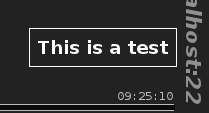
\includegraphics{gateone_displaymessage.png}
\end{flushright}\end{figure}

Displays \emph{message} to the user via a transient pop-up DIV that will appear inside \code{GateOne.prefs.goDiv}.  How long the message lasts can be controlled via \emph{timeout} and \emph{removeTimeout} (which default to 1000 and 5000, respectively).

If \emph{id} is given, it will be prefixed with \code{GateOne.prefs.prefix} and used as the DIV ID for the pop-up.  i.e. \code{GateOne.prefs.prefix+id}.  The default is \code{GateOne.prefs.prefix+"notice"}.

\begin{Verbatim}[commandchars=\\\{\}]
\PYG{g+gp}{\PYGZgt{}\PYGZgt{}\PYGZgt{}} \PYG{n+nx}{GateOne}\PYG{p}{.}\PYG{n+nx}{Visual}\PYG{p}{.}\PYG{n+nx}{displayMessage}\PYG{p}{(}\PYG{l+s+s1}{\PYGZsq{}This is a test.\PYGZsq{}}\PYG{p}{)}\PYG{p}{;}
\end{Verbatim}

\begin{notice}{note}{Note:}
The default is to display the message in the lower-right corner of \code{GateOne.prefs.goDiv} but this can be controlled via CSS.
\end{notice}

\end{fulllineitems}



\begin{fulllineitems}
\phantomsection\label{Developer/js_gateone:GateOne.Visual.handleVisibility}\pysiglinewithargsret{\code{GateOne.Visual.}\bfcode{handleVisibility}}{\emph{e}}{}
This function gets called whenever a tab connected to Gate One becomes visible or invisible.  Triggers the \code{go:visible} and \code{go:invisible} events.

\end{fulllineitems}



\begin{fulllineitems}
\phantomsection\label{Developer/js_gateone:GateOne.Visual.newWorkspace}\pysiglinewithargsret{\code{GateOne.Visual.}\bfcode{newWorkspace}}{}{}
Creates a new workspace on the grid and returns the DOM node that is the new workspace.

If the currently-selected workspace happens to be the application chooser it will be emptied and returned instead of creating a new one.

\end{fulllineitems}



\begin{fulllineitems}
\phantomsection\label{Developer/js_gateone:GateOne.Visual.closeWorkspace}\pysiglinewithargsret{\code{GateOne.Visual.}\bfcode{closeWorkspace}}{\emph{workspace}}{}
Removes the given \emph{workspace} from the `gridwrapper' element and triggers the \code{go:close\_workspace} event.

If \emph{message} (string) is given it will be displayed to the user when the workspace is closed.

\begin{notice}{note}{Note:}
If you're writing an application for Gate One you'll definitely want to attach a function to the \code{go:close\_workspace} event to close your application.
\end{notice}

\end{fulllineitems}



\begin{fulllineitems}
\phantomsection\label{Developer/js_gateone:GateOne.Visual.switchWorkspace}\pysiglinewithargsret{\code{GateOne.Visual.}\bfcode{switchWorkspace}}{\emph{workspace}}{}
Triggers the \code{go:switch\_workspace} event which by default calls {\hyperref[Developer/js_gateone:GateOne.Visual.slideToWorkspace]{\code{GateOne.Visual.slideToWorkspace()}}}.

\begin{notice}{tip}{Tip:}
If you wish to use your own workspace-switching animation just write your own function to handle it and call \code{GateOne.Events.off('go:switch\_workspace', GateOne.Visual.slideToWorkspace); GateOne.Events.on('go:switch\_workspace', yourFunction);}
\end{notice}

\end{fulllineitems}



\begin{fulllineitems}
\phantomsection\label{Developer/js_gateone:GateOne.Visual.cleanupWorkspaces}\pysiglinewithargsret{\code{GateOne.Visual.}\bfcode{cleanupWorkspaces}}{}{}
This gets attached to the `go:cleanup\_workspaces` event which should be triggered by any function that may leave a workspace empty.  It walks through all the workspaces and removes any that are empty.

For example, let's say your app just removed itself from the workspace as a result of a server-controlled action (perhaps a BOFH killed the user's process).  At the end of your \code{closeMyApp()} function you want to put this:

\begin{Verbatim}[commandchars=\\\{\}]
\PYG{n+nx}{GateOne}\PYG{p}{.}\PYG{n+nx}{Events}\PYG{p}{.}\PYG{n+nx}{trigger}\PYG{p}{(}\PYG{l+s+s2}{\PYGZdq{}go:cleanup\PYGZus{}workspaces\PYGZdq{}}\PYG{p}{)}\PYG{p}{;}
\end{Verbatim}

\begin{notice}{note}{Note:}
Make sure you trigger the event instead of calling this function directly so that other attached functions can do their part.
\end{notice}

Why is this mechanism the opposite of everything else where you call the function and that function triggers its associated event?  Embedded mode, of course!  In embedded mode the parent web page may use something other than workspaces (e.g. tabs).  In embedded mode this function never gets attached to the \code{go:cleanup\_workspaces} event so this function will never get called.  This allows the page embedding Gate One to attach its own function to this event to perform an equivalent action (for whatever workspace-like mechanism it is using).

\end{fulllineitems}



\begin{fulllineitems}
\phantomsection\label{Developer/js_gateone:GateOne.Visual.relocateWorkspace}\pysiglinewithargsret{\code{GateOne.Visual.}\bfcode{relocateWorkspace}}{\emph{workspace}, \emph{location}}{}
Relocates the given \emph{workspace} (number) to the given \emph{location} by firing the \code{go:relocate\_workspace} event and \emph{then} closing the workspace (if not already closed).  The given \emph{workspace} and \emph{location} will be passed to the event as the only arguments.

The `data-application' attribute of the DOM node associated with the given \emph{workspace} will be used to determine whether or not the application running on the workspace is relocatable.  It does this by checking the matching application's `\_\_appinfo\_\_.relocatable' attribute.

Applications that support relocation must ensure that they set the appropriate `data-application' attribute on the workspace if they create workspaces on their own.

\end{fulllineitems}



\begin{fulllineitems}
\phantomsection\label{Developer/js_gateone:GateOne.Visual.slideToWorkspace}\pysiglinewithargsret{\code{GateOne.Visual.}\bfcode{slideToWorkspace}}{\emph{workspace}}{}
Slides the view to the given \emph{workspace}.  If \code{GateOne.Visual.noReset} is true, don't reset the grid before switching.

\end{fulllineitems}



\begin{fulllineitems}
\phantomsection\label{Developer/js_gateone:GateOne.Visual.stopIndicator}\pysiglinewithargsret{\code{GateOne.Visual.}\bfcode{stopIndicator}}{\emph{direction}}{}
Displays a visual indicator (appearance determined by theme) that the user cannot slide in given \emph{direction}.  Example:

\begin{Verbatim}[commandchars=\\\{\}]
\PYG{g+gp}{\PYGZgt{}\PYGZgt{}\PYGZgt{}} \PYG{n+nx}{GateOne}\PYG{p}{.}\PYG{n+nx}{Visual}\PYG{p}{.}\PYG{n+nx}{stopIndicator}\PYG{p}{(}\PYG{l+s+s1}{\PYGZsq{}left\PYGZsq{}}\PYG{p}{)}\PYG{p}{;}
\end{Verbatim}

The given \emph{direction} may be one of:  \textbf{left}, \textbf{right}, \textbf{up}, \textbf{down}.

\end{fulllineitems}



\begin{fulllineitems}
\phantomsection\label{Developer/js_gateone:GateOne.Visual.slideLeft}\pysiglinewithargsret{\code{GateOne.Visual.}\bfcode{slideLeft}}{}{}
Slides to the workspace left of the current view.

\end{fulllineitems}



\begin{fulllineitems}
\phantomsection\label{Developer/js_gateone:GateOne.Visual.slideRight}\pysiglinewithargsret{\code{GateOne.Visual.}\bfcode{slideRight}}{}{}
Slides to the workspace right of the current view.

\end{fulllineitems}



\begin{fulllineitems}
\phantomsection\label{Developer/js_gateone:GateOne.Visual.slideDown}\pysiglinewithargsret{\code{GateOne.Visual.}\bfcode{slideDown}}{}{}
Slides the view downward one workspace by pushing all the others up.

\end{fulllineitems}



\begin{fulllineitems}
\phantomsection\label{Developer/js_gateone:GateOne.Visual.slideUp}\pysiglinewithargsret{\code{GateOne.Visual.}\bfcode{slideUp}}{}{}
Slides the view downward one workspace by pushing all the others down.

\end{fulllineitems}



\begin{fulllineitems}
\phantomsection\label{Developer/js_gateone:GateOne.Visual.resetGrid}\pysiglinewithargsret{\code{GateOne.Visual.}\bfcode{resetGrid}}{\emph{animate}}{}
Places all workspaces in their proper position in the grid.  By default this happens instantly with no animations but if \emph{animate} is \code{true} CSS3 transitions will take effect.

\end{fulllineitems}



\begin{fulllineitems}
\phantomsection\label{Developer/js_gateone:GateOne.Visual.gridWorkspaceDragStart}\pysiglinewithargsret{\code{GateOne.Visual.}\bfcode{gridWorkspaceDragStart}}{\emph{e}}{}
Called when the user starts dragging a workspace in grid view; creates drop targets above each workspace and sets up the `dragover', `dragleave', and `drop' events.

This function is also responsible for creating the thumbnail of the workspace being dragged.

\end{fulllineitems}



\begin{fulllineitems}
\phantomsection\label{Developer/js_gateone:GateOne.Visual.gridWorkspaceDragOver}\pysiglinewithargsret{\code{GateOne.Visual.}\bfcode{gridWorkspaceDragOver}}{\emph{e}}{}
Attached to the various drop targets while a workspace is being dragged in grid view; sets the style of the drop target to indicate to the user that the workspace can be dropped there.

\end{fulllineitems}



\begin{fulllineitems}
\phantomsection\label{Developer/js_gateone:GateOne.Visual.gridWorkspaceDragLeave}\pysiglinewithargsret{\code{GateOne.Visual.}\bfcode{gridWorkspaceDragLeave}}{\emph{e}}{}
Attached to the various drop targets while a workspace is being dragged in grid view; sets the background color of the drop target back to `transparent' to give the user a clear visual indiciation that the drag is no longer above the drop target.

\end{fulllineitems}



\begin{fulllineitems}
\phantomsection\label{Developer/js_gateone:GateOne.Visual.gridWorkspaceDrop}\pysiglinewithargsret{\code{GateOne.Visual.}\bfcode{gridWorkspaceDrop}}{\emph{e}}{}
Attached to the various drop targets while a workspace is being dragged in grid view; handles the `drop' of a workspace on to another.  Will swap the dragged workspace with the one to which it was dropped by calling {\hyperref[Developer/js_gateone:GateOne.Visual.swapWorkspaces]{\code{GateOne.Visual.swapWorkspaces()}}}

\end{fulllineitems}



\begin{fulllineitems}
\phantomsection\label{Developer/js_gateone:GateOne.Visual.swapWorkspaces}\pysiglinewithargsret{\code{GateOne.Visual.}\bfcode{swapWorkspaces}}{\emph{ws1}, \emph{ws2}}{}
Swaps the location of the given workspaces in the grid and fires the \code{go:swapped\_workspaces} event with \emph{ws1} and \emph{ws2} as the arguments.
\begin{quote}\begin{description}
\item[{Ws1 number}] \leavevmode
The workspace number.

\item[{Ws2 number}] \leavevmode
The other workspace number.

\end{description}\end{quote}

\end{fulllineitems}



\begin{fulllineitems}
\phantomsection\label{Developer/js_gateone:GateOne.Visual.toggleGridView}\pysiglinewithargsret{\code{GateOne.Visual.}\bfcode{toggleGridView}}{\optional{\emph{goBack}}}{}
Brings up the workspace grid view or returns to full-size.

If \emph{goBack} is false, don't bother switching back to the previously-selected workspace

\end{fulllineitems}



\begin{fulllineitems}
\phantomsection\label{Developer/js_gateone:GateOne.Visual.createGrid}\pysiglinewithargsret{\code{GateOne.Visual.}\bfcode{createGrid}}{\emph{id}, \emph{workspaceNames}}{}
Creates a container for all the workspaces and optionally pre-creates workspaces using \emph{workspaceNames}.

\emph{id} will be the ID of the resulting grid (e.g. ``gridwrapper'').

\emph{workspaceNames} is expected to be a list of DOM IDs.

\end{fulllineitems}



\begin{fulllineitems}
\phantomsection\label{Developer/js_gateone:GateOne.Visual.serverMessageAction}\pysiglinewithargsret{\code{GateOne.Visual.}\bfcode{serverMessageAction}}{\emph{message}}{}
Attached to the \code{go:notice} WebSocket action; displays a given \emph{message} from the Gate One server as a transient pop-up using {\hyperref[Developer/js_gateone:GateOne.Visual.displayMessage]{\code{GateOne.Visual.displayMessage()}}}.

\end{fulllineitems}



\begin{fulllineitems}
\phantomsection\label{Developer/js_gateone:GateOne.Visual.userMessageAction}\pysiglinewithargsret{\code{GateOne.Visual.}\bfcode{userMessageAction}}{\emph{message}}{}
Attached to the \code{go:user\_message} WebSocket action; displays a given \emph{message} as a transient pop-up using {\hyperref[Developer/js_gateone:GateOne.Visual.displayMessage]{\code{GateOne.Visual.displayMessage()}}}.

\begin{notice}{note}{Note:}
This will likely change to include/use additional metadata in the future (such as: from, to, etc)
\end{notice}

\end{fulllineitems}



\begin{fulllineitems}
\phantomsection\label{Developer/js_gateone:GateOne.Visual.dialog}\pysiglinewithargsret{\code{GateOne.Visual.}\bfcode{dialog}}{\emph{title}, \emph{content}\optional{, \emph{options}}}{}
Creates an in-page dialog with the given \emph{title} and \emph{content}.  Returns a function that will close the dialog when called.

Dialogs can be moved around and closed at-will by the user with a clearly visible title bar that is always present.

All dialogs are placed within the \code{GateOne.prefs.goDiv} container but have their position set to `fixed' so they can be moved anywhere on the page (even outside of the container where Gate One resides).
\begin{quote}\begin{description}
\item[{Arguments}] \leavevmode\begin{itemize}
\item {} 
\textbf{title} (\emph{string}) -- Will appear at the top of the dialog.

\item {} 
\textbf{content} (\emph{stringOrNode}) -- String or JavaScript DOM node - The content of the dialog.

\item {} 
\textbf{options} (\emph{object}) -- An associative array of parameters that change the look and/or behavior of the dialog.  See below.

\end{itemize}

\end{description}\end{quote}

\textbf{Options}
\begin{quote}
\begin{quote}\begin{description}
\item[{events}] \leavevmode
An object containing DOM events that will be attached to the dialog node.  Example: \code{\{'mousedown': someFunction\}}.  There are a few special/simulated events of which you may also attach: `focused', `closed', `opened', `resized', and `moved'.  Except for `close', these special event functions will be passed the dialog node as the only argument.

\item[{resizable}] \leavevmode
If set to \code{false} the dialog will not be resizable (all dialogs are resizable by default).  Note that if a dialog may not be resized it will also not be maximizable.

\item[{maximizable}] \leavevmode
If set to \code{false} the dialog will not have a maximize icon.

\item[{minimizable}] \leavevmode
If set to \code{false} the dialog will not have a minimize icon.

\item[{maximize}] \leavevmode
Open the dialog maximized.

\item[{above}] \leavevmode
If set to \code{true} the dialog will be kept above others.

\item[{data}] \leavevmode
(object) If given, any contained properties will be set as `data-*' attributes on the dialogContainer.

\item[{where}] \leavevmode
If given, the dialog will be placed here (DOM node or querySelector-like string) and will only be able to movable within the parent element.  Otherwise the dialog will be appended to the Gate One container (\code{GateOne.node}) and will be movable anywhere on the page.

\item[{noEsc}] \leavevmode
If \code{true} the dialog will not watch for the ESC key to close itself.

\item[{noTransitions}] \leavevmode
If \code{true} CSS3 transitions will not be enabled for this dialog.

\item[{class}] \leavevmode
Any additional CSS classes you wish to add to the dialog (space-separated).

\item[{style}] \leavevmode
Any CSS you wish to apply to the dialog.  Example:  \code{\{'style': \{'width': '50\%', 'height': '25\%'\}\}}

\end{description}\end{quote}
\end{quote}

\end{fulllineitems}



\begin{fulllineitems}
\phantomsection\label{Developer/js_gateone:GateOne.Visual.alert}\pysiglinewithargsret{\code{GateOne.Visual.}\bfcode{alert}}{\emph{title}, \emph{message}\optional{, \emph{callback}}}{}~\begin{quote}\begin{description}
\item[{Arguments}] \leavevmode\begin{itemize}
\item {} 
\textbf{title} (\emph{string}) -- Title of the dialog that will be displayed.

\item {} 
\textbf{message} -- An HTML-formatted string or a DOM node; Main content of the alert dialog.

\item {} 
\textbf{callback} (\emph{function}) -- A function that will be called after the user clicks ``OK''.

\end{itemize}

\end{description}\end{quote}
\begin{figure}[htbp]\begin{flushright}

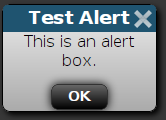
\includegraphics{gateone_alert.png}
\end{flushright}\end{figure}

Displays a dialog using the given \emph{title} containing the given \emph{message} along with an OK button.  When the OK button is clicked, \emph{callback} will be called.

\begin{Verbatim}[commandchars=\\\{\}]
\PYG{g+gp}{\PYGZgt{}\PYGZgt{}\PYGZgt{}} \PYG{n+nx}{GateOne}\PYG{p}{.}\PYG{n+nx}{Visual}\PYG{p}{.}\PYG{n+nx}{alert}\PYG{p}{(}\PYG{l+s+s1}{\PYGZsq{}Test Alert\PYGZsq{}}\PYG{p}{,} \PYG{l+s+s1}{\PYGZsq{}This is an alert box.\PYGZsq{}}\PYG{p}{)}\PYG{p}{;}
\end{Verbatim}

\begin{notice}{note}{Note:}
This function is meant to be a less-intrusive form of JavaScript's alert().
\end{notice}

\end{fulllineitems}



\begin{fulllineitems}
\phantomsection\label{Developer/js_gateone:GateOne.Visual.showDock}\pysiglinewithargsret{\code{GateOne.Visual.}\bfcode{showDock}}{\emph{name}}{}
Opens up the given \emph{name} for the user to view.  If the dock does not already exist it will be created and added to the toolbar.

\end{fulllineitems}



\begin{fulllineitems}
\phantomsection\label{Developer/js_gateone:GateOne.Visual.toggleOverlay}\pysiglinewithargsret{\code{GateOne.Visual.}\bfcode{toggleOverlay}}{}{}
Toggles the overlay that visually indicates whether or not Gate One is ready for input.  Normally this function gets called automatically by \code{GateOne.Input.capture()} and \code{GateOne.Input.disableCapture()} which are attached to \code{mousedown} and \code{blur} events, respectively.

\end{fulllineitems}



\begin{fulllineitems}
\phantomsection\label{Developer/js_gateone:GateOne.Visual.enableOverlay}\pysiglinewithargsret{\code{GateOne.Visual.}\bfcode{enableOverlay}}{}{}
Displays an overlay above Gate One on the page that `greys it out' to indicate it does not have focus.  If the overlay is already present it will be left as-is.

The state of the overlay is tracked via the \code{GateOne.Visual.overlay} variable.

\end{fulllineitems}



\begin{fulllineitems}
\phantomsection\label{Developer/js_gateone:GateOne.Visual.disableOverlay}\pysiglinewithargsret{\code{GateOne.Visual.}\bfcode{disableOverlay}}{}{}
Removes the overlay above Gate One (if present).

The state of the overlay is tracked via the \code{GateOne.Visual.overlay} variable.

\end{fulllineitems}


\end{fulllineitems}



\begin{fulllineitems}
\phantomsection\label{Developer/js_gateone:GateOne.Storage}\pysigline{\code{GateOne.}\bfcode{Storage}}
An object for opening and manipulating \href{https://developer.mozilla.org/en-US/docs/IndexedDB}{IndexedDB} databases with fallback to \href{https://developer.mozilla.org/en-US/docs/Web/Guide/DOM/Storage\#localStorage}{localStorage}.


\begin{fulllineitems}
\phantomsection\label{Developer/js_gateone:GateOne.Storage.dbObject}\pysigline{\code{GateOne.Storage.}\bfcode{dbObject}}~\begin{quote}\begin{description}
\item[{Arguments}] \leavevmode\begin{itemize}
\item {} 
\textbf{DB} (\emph{string}) -- A string representing the name of the database you want to open.

\end{itemize}

\end{description}\end{quote}

Returns a new object that can be used to store and retrieve data stored in the given database.  Normally you'll get access to this object through the {\hyperref[Developer/js_gateone:GateOne.Storage.openDB]{\code{GateOne.Storage.openDB()}}} function (it gets passed as the argument to your callback).


\begin{fulllineitems}
\phantomsection\label{Developer/js_gateone:GateOne.Storage.dbObject.get}\pysiglinewithargsret{\code{GateOne.Storage.dbObject.}\bfcode{get}}{\emph{storeName}, \emph{key}, \emph{callback}}{}
Retrieves the object matching the given \emph{key} in the given object store (\emph{storeName}) and calls \emph{callback} with the result.

\end{fulllineitems}



\begin{fulllineitems}
\phantomsection\label{Developer/js_gateone:GateOne.Storage.dbObject.put}\pysiglinewithargsret{\code{GateOne.Storage.dbObject.}\bfcode{put}}{\emph{storeName}, \emph{value}\optional{, \emph{callback}}}{}
Adds \emph{value} to the given object store (\emph{storeName}).  If given, calls \emph{callback} with \emph{value} as the only argument.

\end{fulllineitems}



\begin{fulllineitems}
\phantomsection\label{Developer/js_gateone:GateOne.Storage.dbObject.del}\pysiglinewithargsret{\code{GateOne.Storage.dbObject.}\bfcode{del}}{\emph{storeName}, \emph{key}\optional{, \emph{callback}}}{}
Deletes the object matching \emph{key} from the given object store (\emph{storeName}).  If given, calls \emph{callback} when the transaction is complete.

\end{fulllineitems}



\begin{fulllineitems}
\phantomsection\label{Developer/js_gateone:GateOne.Storage.dbObject.dump}\pysiglinewithargsret{\code{GateOne.Storage.dbObject.}\bfcode{dump}}{\emph{storeName}, \emph{callback}}{}
Retrieves all objects in the given object store (\emph{storeName}) and calls \emph{callback} with the result.

\end{fulllineitems}


\end{fulllineitems}



\begin{fulllineitems}
\phantomsection\label{Developer/js_gateone:GateOne.Storage.init}\pysiglinewithargsret{\code{GateOne.Storage.}\bfcode{init}}{}{}
Doesn't do anything (most init stuff for this module needs to happen before everything else loads).

\end{fulllineitems}



\begin{fulllineitems}
\phantomsection\label{Developer/js_gateone:GateOne.Storage.cacheReady}\pysiglinewithargsret{\code{GateOne.Storage.}\bfcode{cacheReady}}{}{}
Called when the fileCache DB has completed openining/initialization.  Just sets \code{GateOne.Storage.fileCacheReady} to \code{true}.

\end{fulllineitems}



\begin{fulllineitems}
\phantomsection\label{Developer/js_gateone:GateOne.Storage.cacheJS}\pysiglinewithargsret{\code{GateOne.Storage.}\bfcode{cacheJS}}{\emph{fileObj}}{}
Stores the given \emph{fileObj} in the `fileCache' database in the `js' store.

\begin{notice}{note}{Note:}
Normally this only gets run from {\hyperref[Developer/js_gateone:GateOne.Utils.loadJSAction]{\code{GateOne.Utils.loadJSAction()}}}.
\end{notice}

\end{fulllineitems}



\begin{fulllineitems}
\phantomsection\label{Developer/js_gateone:GateOne.Storage.uncacheJS}\pysiglinewithargsret{\code{GateOne.Storage.}\bfcode{uncacheJS}}{\emph{fileObj}}{}
Removes the given \emph{fileObj} from the cache (if present).

\begin{notice}{note}{Note:}
This will fail silently if the given \emph{fileObj} does not exist in the cache.
\end{notice}

\end{fulllineitems}



\begin{fulllineitems}
\phantomsection\label{Developer/js_gateone:GateOne.Storage.cacheStyle}\pysiglinewithargsret{\code{GateOne.Storage.}\bfcode{cacheStyle}}{\emph{fileObj}, \emph{kind}}{}
Stores the given \emph{fileObj} in the `fileCache' database in the store associated with the given \emph{kind} of stylesheet.  Stylesheets are divided into different `kind' categories because some need special handling (e.g. themes need to be hot-swappable).

\begin{notice}{note}{Note:}
Normally this only gets run from {\hyperref[Developer/js_gateone:GateOne.Utils.loadStyleAction]{\code{GateOne.Utils.loadStyleAction()}}}.
\end{notice}

\end{fulllineitems}



\begin{fulllineitems}
\phantomsection\label{Developer/js_gateone:GateOne.Storage.uncacheStyle}\pysiglinewithargsret{\code{GateOne.Storage.}\bfcode{uncacheStyle}}{\emph{fileObj}, \emph{kind}}{}
Removes the given \emph{fileObj} from the cache matching \emph{kind} (if present).  The \emph{kind} argument must be one of `css', `theme', or `print'.

\begin{notice}{note}{Note:}
This will fail silently if the given \emph{fileObj} does not exist in the cache.
\end{notice}

\end{fulllineitems}



\begin{fulllineitems}
\phantomsection\label{Developer/js_gateone:GateOne.Storage.cacheExpiredAction}\pysiglinewithargsret{\code{GateOne.Storage.}\bfcode{cacheExpiredAction}}{\emph{message}}{}
Attached to the \code{go:cache\_expired} WebSocket action; given a list of \emph{message{[}'filenames'{]}}, removes them from the file cache.

\end{fulllineitems}



\begin{fulllineitems}
\phantomsection\label{Developer/js_gateone:GateOne.Storage.fileCheckAction}\pysiglinewithargsret{\code{GateOne.Storage.}\bfcode{fileCheckAction}}{\emph{message}}{}
This gets attached to the \code{go:file\_sync} WebSocket action; given a list of file objects which includes their modification times (\emph{message{[}'files'{]}}) it will either load the file from the `fileCache' database or request the file be delivered via the (server-side) `go:file\_request` WebSocket action.

\begin{notice}{note}{Note:}
Expects the `fileCache' database be open and ready (normally it gets opened/initialized in {\hyperref[Developer/js_gateone:GateOne.initialize]{\code{GateOne.initialize()}}}).
\end{notice}

\end{fulllineitems}



\begin{fulllineitems}
\phantomsection\label{Developer/js_gateone:GateOne.Storage.onerror}\pysiglinewithargsret{\code{GateOne.Storage.}\bfcode{onerror}}{\emph{e}}{}
Attached as the errorback function in various storage operations; logs the given error (\emph{e}).

\end{fulllineitems}



\begin{fulllineitems}
\phantomsection\label{Developer/js_gateone:GateOne.Storage._upgradeDB}\pysiglinewithargsret{\code{GateOne.Storage.}\bfcode{\_upgradeDB}}{\emph{trans}\optional{, \emph{callback}}}{}
DB version upgrade function attached to the \code{onupgradeneeded} event.  It creates our object store(s).

If \emph{callback} is given it will be called when the transaction is complete.

\end{fulllineitems}



\begin{fulllineitems}
\phantomsection\label{Developer/js_gateone:GateOne.Storage.openDB}\pysiglinewithargsret{\code{GateOne.Storage.}\bfcode{openDB}}{\emph{DB}\optional{, \emph{callback}\optional{, \emph{model}\optional{, \emph{version}}}}}{}
Opens the given database (\emph{DB}) for use and stores a reference to it as \code{GateOne.Storage.databases{[}DB{]}}.

If \emph{callback} is given, will execute it after the database has been opened successfuly.

If this is the first time we're opening this database a \emph{model} must be given.  Also, if the database already exists, the \emph{model} argument will be ignored so it is safe to pass it with every call to this function.

If provided, the \emph{version} of the database will be set.  Otherwise it will be set to 1.

Example usage:

\begin{Verbatim}[commandchars=\\\{\}]
\PYG{k+kd}{var} \PYG{n+nx}{model} \PYG{o}{=} \PYG{p}{\PYGZob{}}\PYG{l+s+s1}{\PYGZsq{}BookmarksDB\PYGZsq{}}\PYG{o}{:} \PYG{p}{\PYGZob{}}\PYG{l+s+s1}{\PYGZsq{}bookmarks\PYGZsq{}}\PYG{o}{:} \PYG{p}{\PYGZob{}}\PYG{n+nx}{keyPath}\PYG{o}{:} \PYG{l+s+s2}{\PYGZdq{}url\PYGZdq{}}\PYG{p}{\PYGZcb{}}\PYG{p}{,} \PYG{l+s+s1}{\PYGZsq{}tags\PYGZsq{}}\PYG{o}{:} \PYG{p}{\PYGZob{}}\PYG{n+nx}{keyPath}\PYG{o}{:} \PYG{l+s+s2}{\PYGZdq{}name\PYGZdq{}}\PYG{p}{\PYGZcb{}}\PYG{p}{\PYGZcb{}}\PYG{p}{\PYGZcb{}}\PYG{p}{;}
\PYG{n+nx}{GateOne}\PYG{p}{.}\PYG{n+nx}{Storage}\PYG{p}{.}\PYG{n+nx}{openDB}\PYG{p}{(}\PYG{l+s+s1}{\PYGZsq{}somedb\PYGZsq{}}\PYG{p}{,} \PYG{k+kd}{function}\PYG{p}{(}\PYG{n+nx}{dbObj}\PYG{p}{)} \PYG{p}{\PYGZob{}}\PYG{n+nx}{console}\PYG{p}{.}\PYG{n+nx}{log}\PYG{p}{(}\PYG{n+nx}{dbObj}\PYG{p}{)}\PYG{p}{;}\PYG{p}{\PYGZcb{}}\PYG{p}{,} \PYG{n+nx}{model}\PYG{p}{)}\PYG{p}{;}
\PYG{c+c1}{// Note that after this DB is opened the IDBDatabase object will be available via GateOne.Storage.databases[\PYGZsq{}somedb\PYGZsq{}]}
\end{Verbatim}

\end{fulllineitems}



\begin{fulllineitems}
\phantomsection\label{Developer/js_gateone:GateOne.Storage.clearDatabase}\pysiglinewithargsret{\code{GateOne.Storage.}\bfcode{clearDatabase}}{\emph{DB}\optional{, \emph{storeName}}}{}
Clears the contents of the given \emph{storeName} in the given database (\emph{DB}).  AKA ``the nuclear option.''

If a \emph{storeName} is not given the whole database will be deleted.

\end{fulllineitems}


\end{fulllineitems}



\begin{fulllineitems}
\phantomsection\label{Developer/js_gateone:GateOne.User}\pysigline{\code{GateOne.}\bfcode{User}}
The User module is for things like logging out, synchronizing preferences with the server, and it is also meant to provide hooks for plugins to tie into so that actions can be taken when user-specific events occur.

The following WebSocket actions are attached to functions provided by \code{GateOne.User}:
\begin{quote}

\begin{tabulary}{\linewidth}{|L|L|}
\hline
\textsf{\relax 
Action
} & \textsf{\relax 
Function
}\\
\hline
\code{go:gateone\_user}
 & 
{\hyperref[Developer/js_gateone:GateOne.User.storeSessionAction]{\code{GateOne.User.storeSessionAction()}}}
\\
\hline
\code{go:set\_username}
 & 
{\hyperref[Developer/js_gateone:GateOne.User.setUsernameAction]{\code{GateOne.User.setUsernameAction()}}}
\\
\hline
\code{go:applications}
 & 
{\hyperref[Developer/js_gateone:GateOne.User.applicationsAction]{\code{GateOne.User.applicationsAction()}}}
\\
\hline
\code{go:user\_list}
 & 
{\hyperref[Developer/js_gateone:GateOne.User.userListAction]{\code{GateOne.User.userListAction()}}}
\\
\hline\end{tabulary}

\end{quote}


\begin{fulllineitems}
\phantomsection\label{Developer/js_gateone:GateOne.User.init}\pysiglinewithargsret{\code{GateOne.User.}\bfcode{init}}{}{}
Adds the user's ID (aka UPN) to the prefs panel along with a logout link.

\end{fulllineitems}



\begin{fulllineitems}
\phantomsection\label{Developer/js_gateone:GateOne.User.workspaceApp}\pysiglinewithargsret{\code{GateOne.User.}\bfcode{workspaceApp}}{\emph{workspace}}{}
Attached to the `go:switch\_workspace` event; sets \code{GateOne.User.activeApplication} to whatever application is attached to the \code{data-application} attribute on the provided \emph{workspace}.

\end{fulllineitems}



\begin{fulllineitems}
\phantomsection\label{Developer/js_gateone:GateOne.User.setActiveApp}\pysiglinewithargsret{\code{GateOne.User.}\bfcode{setActiveApp}}{\emph{app}}{}
Sets \code{GateOne.User.activeApplication} the given \emph{app}.

\begin{notice}{note}{Note:}
The \emph{app} argument is case-insensitive.  For example, if you pass `terminal' it will set the active application to `Terminal' (which is the name inside \code{GateOne.User.applications}).
\end{notice}

\end{fulllineitems}



\begin{fulllineitems}
\phantomsection\label{Developer/js_gateone:GateOne.User.setUsernameAction}\pysiglinewithargsret{\code{GateOne.User.}\bfcode{setUsernameAction}}{\emph{username}}{}
Sets \code{GateOne.User.username} to \emph{username}.  Also triggers the \code{go:user\_login} event with the username as the only argument.

\begin{notice}{tip}{Tip:}
If you want to call a function after the user has successfully loaded Gate One and authenticated attach it to the \code{go:user\_login} event.
\end{notice}

\end{fulllineitems}



\begin{fulllineitems}
\phantomsection\label{Developer/js_gateone:GateOne.User.logout}\pysiglinewithargsret{\code{GateOne.User.}\bfcode{logout}}{\emph{redirectURL}}{}
This function will log the user out by deleting all Gate One cookies and forcing them to re-authenticate.  By default this is what is attached to the `logout' link in the preferences panel.

If provided, \emph{redirectURL} will be used to automatically redirect the user to the given URL after they are logged out (as opposed to just reloading the main Gate One page).

Triggers the \code{go:user\_logout} event with the username as the only argument.

\end{fulllineitems}



\begin{fulllineitems}
\phantomsection\label{Developer/js_gateone:GateOne.User.storeSessionAction}\pysiglinewithargsret{\code{GateOne.User.}\bfcode{storeSessionAction}}{\emph{message}}{}
This gets attached to the \code{go:gateone\_user} \href{https://developer.mozilla.org/en/WebSockets/WebSockets\_reference/WebSocket}{WebSocket} action in {\hyperref[Developer/js_gateone:GateOne.Net.actions]{\code{GateOne.Net.actions}}}.  It stores the incoming (encrypted) `gateone\_user' session data in localStorage in a nearly identical fashion to how it gets stored in the `gateone\_user' cookie.

\begin{notice}{note}{Note:}
The reason for storing data in localStorage instead of in the cookie is so that applications embedding Gate One can remain authenticated to the user without having to deal with the cross-origin limitations of cookies.
\end{notice}

\end{fulllineitems}



\begin{fulllineitems}
\phantomsection\label{Developer/js_gateone:GateOne.User.applicationsAction}\pysiglinewithargsret{\code{GateOne.User.}\bfcode{applicationsAction}}{}{}
Sets \code{GateOne.User.applications} to the given list of \emph{apps} (which is the list of applications the user is allowed to run).

\end{fulllineitems}



\begin{fulllineitems}
\phantomsection\label{Developer/js_gateone:GateOne.User.preference}\pysiglinewithargsret{\code{GateOne.User.}\bfcode{preference}}{\emph{title}, \emph{content}}{}
Adds a new section to the preferences panel using the given \emph{title} and \emph{content}.  The \emph{title} will be used to create a link that will bring up \emph{content}.  The \emph{content} will be placed inside the preferences form.

To place a preference under a subsection (e.g. Terminal -\textgreater{} SSH) provide the \emph{title} like so:  ``Terminal:SSH''.

If \emph{callback} is given it will be attacheed to the ``go:save\_prefs'' event.

\end{fulllineitems}



\begin{fulllineitems}
\phantomsection\label{Developer/js_gateone:GateOne.User.listUsers}\pysiglinewithargsret{\code{GateOne.User.}\bfcode{listUsers}}{\optional{\emph{callback}}}{}
Sends the \code{terminal:list\_users} WebSocket action to the server which will reply with the \code{go:user\_list} WebSocket action containing a list of all users that are currently connected.  Only users which are allowed to list users via the ``list\_users'' policy will be able to perform this action.

If a \emph{callback} is given it will be called with the list of users (once it arrives from the server).

\end{fulllineitems}



\begin{fulllineitems}
\phantomsection\label{Developer/js_gateone:GateOne.User.userListAction}\pysiglinewithargsret{\code{GateOne.User.}\bfcode{userListAction}}{}{}
Attached to the \code{go:user\_list} WebSocket action; sets \code{GateOne.User.userList} and triggers the \code{go:user\_list} event passing the list of users as the only argument.

\end{fulllineitems}


\end{fulllineitems}



\begin{fulllineitems}
\phantomsection\label{Developer/js_gateone:GateOne.Events}\pysigline{\code{GateOne.}\bfcode{Events}}
An object for event-specific stuff.  Inspired by Backbone.js Events.


\begin{fulllineitems}
\phantomsection\label{Developer/js_gateone:GateOne.Events.on}\pysiglinewithargsret{\code{GateOne.Events.}\bfcode{on}}{\emph{events}, \emph{callback}\optional{, \emph{context}\optional{, \emph{times}}}}{}
Adds the given \emph{callback} / \emph{context} combination to the given \emph{events}; to be called when the given \emph{events} are triggered.
\begin{quote}\begin{description}
\item[{Arguments}] \leavevmode\begin{itemize}
\item {} 
\textbf{events} (\emph{string}) -- A space-separated list of events that will have the given \emph{callback} / \emph{context} attached.

\item {} 
\textbf{callback} (\emph{function}) -- The function to be called when the given \emph{event} is triggered.

\item {} 
\textbf{context} (\emph{object}) -- An object that will be bound to \emph{callback} as \code{this} when it is called.

\item {} 
\textbf{times} (\emph{integer}) -- The number of times this callback will be called before it is removed from the given \emph{event}.

\end{itemize}

\end{description}\end{quote}

Examples:

\begin{Verbatim}[commandchars=\\\{\}]
\PYG{g+gp}{\PYGZgt{}\PYGZgt{}\PYGZgt{}} \PYG{c+c1}{// A little test function}
\PYG{g+gp}{\PYGZgt{}\PYGZgt{}\PYGZgt{}} \PYG{k+kd}{var} \PYG{n+nx}{testFunc} \PYG{o}{=} \PYG{k+kd}{function}\PYG{p}{(}\PYG{n+nx}{args}\PYG{p}{)} \PYG{p}{\PYGZob{}} \PYG{n+nx}{console}\PYG{p}{.}\PYG{n+nx}{log}\PYG{p}{(}\PYG{l+s+s1}{\PYGZsq{}args: \PYGZsq{}} \PYG{o}{+} \PYG{n+nx}{args} \PYG{o}{+} \PYG{l+s+s1}{\PYGZsq{}, this.foo: \PYGZsq{}} \PYG{o}{+} \PYG{k}{this}\PYG{p}{.}\PYG{n+nx}{foo}\PYG{p}{)} \PYG{p}{\PYGZcb{}}\PYG{p}{;}
\PYG{g+gp}{\PYGZgt{}\PYGZgt{}\PYGZgt{}} \PYG{c+c1}{// Call testFunc whenever the \PYGZdq{}test\PYGZus{}event\PYGZdq{} event is triggered}
\PYG{g+gp}{\PYGZgt{}\PYGZgt{}\PYGZgt{}} \PYG{n+nx}{GateOne}\PYG{p}{.}\PYG{n+nc}{Event}\PYG{n+nx}{s}\PYG{p}{.}\PYG{n+nx}{on}\PYG{p}{(}\PYG{l+s+s2}{\PYGZdq{}test\PYGZus{}event\PYGZdq{}}\PYG{p}{,} \PYG{n+nx}{testFunc}\PYG{p}{)}\PYG{p}{;}
\PYG{g+gp}{\PYGZgt{}\PYGZgt{}\PYGZgt{}} \PYG{c+c1}{// Fire the test\PYGZus{}event with \PYGZsq{}an argument\PYGZsq{} as the only argument}
\PYG{g+gp}{\PYGZgt{}\PYGZgt{}\PYGZgt{}} \PYG{n+nx}{GateOne}\PYG{p}{.}\PYG{n+nc}{Event}\PYG{n+nx}{s}\PYG{p}{.}\PYG{n+nx}{trigger}\PYG{p}{(}\PYG{l+s+s2}{\PYGZdq{}test\PYGZus{}event\PYGZdq{}}\PYG{p}{,} \PYG{l+s+s1}{\PYGZsq{}an argument\PYGZsq{}}\PYG{p}{)}\PYG{p}{;}
\PYG{g+go}{args}\PYG{g+go}{:}\PYG{g+go}{ }\PYG{g+go}{an}\PYG{g+go}{ }\PYG{g+go}{argument}\PYG{g+go}{,}\PYG{g+go}{ }\PYG{g+go}{this}\PYG{g+go}{.}\PYG{g+go}{foo}\PYG{g+go}{:}\PYG{g+go}{ }\PYG{g+go}{undefined}
\PYG{g+gp}{\PYGZgt{}\PYGZgt{}\PYGZgt{}} \PYG{c+c1}{// Remove the event so we can change it}
\PYG{g+gp}{\PYGZgt{}\PYGZgt{}\PYGZgt{}} \PYG{n+nx}{GateOne}\PYG{p}{.}\PYG{n+nc}{Event}\PYG{n+nx}{s}\PYG{p}{.}\PYG{n+nx}{off}\PYG{p}{(}\PYG{l+s+s2}{\PYGZdq{}test\PYGZus{}event\PYGZdq{}}\PYG{p}{,} \PYG{n+nx}{testFunc}\PYG{p}{)}\PYG{p}{;}
\PYG{g+gp}{\PYGZgt{}\PYGZgt{}\PYGZgt{}} \PYG{c+c1}{// Now let\PYGZsq{}s pass in a context object}
\PYG{g+gp}{\PYGZgt{}\PYGZgt{}\PYGZgt{}} \PYG{n+nx}{GateOne}\PYG{p}{.}\PYG{n+nc}{Event}\PYG{n+nx}{s}\PYG{p}{.}\PYG{n+nx}{on}\PYG{p}{(}\PYG{l+s+s2}{\PYGZdq{}test\PYGZus{}event\PYGZdq{}}\PYG{p}{,} \PYG{n+nx}{testFunc}\PYG{p}{,} \PYG{p}{\PYGZob{}}\PYG{l+s+s1}{\PYGZsq{}foo\PYGZsq{}}\PYG{o}{:} \PYG{l+s+s1}{\PYGZsq{}bar\PYGZsq{}}\PYG{p}{\PYGZcb{}}\PYG{p}{)}\PYG{p}{;}
\PYG{g+gp}{\PYGZgt{}\PYGZgt{}\PYGZgt{}} \PYG{c+c1}{// Now fire it just like before}
\PYG{g+gp}{\PYGZgt{}\PYGZgt{}\PYGZgt{}} \PYG{n+nx}{GateOne}\PYG{p}{.}\PYG{n+nc}{Event}\PYG{n+nx}{s}\PYG{p}{.}\PYG{n+nx}{trigger}\PYG{p}{(}\PYG{l+s+s2}{\PYGZdq{}test\PYGZus{}event\PYGZdq{}}\PYG{p}{,} \PYG{l+s+s1}{\PYGZsq{}an argument\PYGZsq{}}\PYG{p}{)}\PYG{p}{;}
\PYG{g+go}{args}\PYG{g+go}{:}\PYG{g+go}{ }\PYG{g+go}{an}\PYG{g+go}{ }\PYG{g+go}{argument}\PYG{g+go}{,}\PYG{g+go}{ }\PYG{g+go}{this}\PYG{g+go}{.}\PYG{g+go}{foo}\PYG{g+go}{:}\PYG{g+go}{ }\PYG{g+go}{bar}
\end{Verbatim}

\end{fulllineitems}



\begin{fulllineitems}
\phantomsection\label{Developer/js_gateone:GateOne.Events.off}\pysiglinewithargsret{\code{GateOne.Events.}\bfcode{off}}{\emph{events}, \emph{callback}\optional{, \emph{context}}}{}
Removes the given \emph{callback} / \emph{context} combination from the given \emph{events}
\begin{quote}\begin{description}
\item[{Arguments}] \leavevmode\begin{itemize}
\item {} 
\textbf{events} (\emph{string}) -- A space-separated list of events.

\item {} 
\textbf{callback} (\emph{function}) -- The function that's attached to the given events to be removed.

\item {} 
\textbf{context} (\emph{object}) -- The context attached to the given event/callback to be removed.

\end{itemize}

\end{description}\end{quote}

Example:

\begin{Verbatim}[commandchars=\\\{\}]
\PYG{g+gp}{\PYGZgt{}\PYGZgt{}\PYGZgt{}} \PYG{n+nx}{GateOne}\PYG{p}{.}\PYG{n+nc}{Event}\PYG{n+nx}{s}\PYG{p}{.}\PYG{n+nx}{off}\PYG{p}{(}\PYG{l+s+s2}{\PYGZdq{}new\PYGZus{}terminal\PYGZdq{}}\PYG{p}{,} \PYG{n+nx}{someFunction}\PYG{p}{)}\PYG{p}{;}
\end{Verbatim}

\end{fulllineitems}



\begin{fulllineitems}
\phantomsection\label{Developer/js_gateone:GateOne.Events.once}\pysiglinewithargsret{\code{GateOne.Events.}\bfcode{once}}{\emph{events}, \emph{callback}\optional{, \emph{context}}}{}
A shortcut that performs the equivalent of \code{GateOne.Events.on(events, callback, context, 1)}.

\end{fulllineitems}



\begin{fulllineitems}
\phantomsection\label{Developer/js_gateone:GateOne.Events.trigger}\pysiglinewithargsret{\code{GateOne.Events.}\bfcode{trigger}}{\emph{events}}{}
Triggers the given \emph{events}.  Any additional provided arguments will be passed to the callbacks attached to the given events.
\begin{quote}\begin{description}
\item[{Arguments}] \leavevmode\begin{itemize}
\item {} 
\textbf{events} (\emph{string}) -- A space-separated list of events to trigger

\end{itemize}

\end{description}\end{quote}

Example:

\begin{Verbatim}[commandchars=\\\{\}]
\PYG{g+gp}{\PYGZgt{}\PYGZgt{}\PYGZgt{}} \PYG{c+c1}{// The \PYGZsq{}1\PYGZsq{} below will be passed to each callback as the only argument}
\PYG{g+gp}{\PYGZgt{}\PYGZgt{}\PYGZgt{}} \PYG{n+nx}{GateOne}\PYG{p}{.}\PYG{n+nc}{Event}\PYG{n+nx}{s}\PYG{p}{.}\PYG{n+nx}{trigger}\PYG{p}{(}\PYG{l+s+s2}{\PYGZdq{}new\PYGZus{}terminal\PYGZdq{}}\PYG{p}{,} \PYG{l+m+mi}{1}\PYG{p}{)}\PYG{p}{;}
\end{Verbatim}

\end{fulllineitems}


\end{fulllineitems}


\end{fulllineitems}

\index{GateOne.restoreDefaults() (GateOne method)}

\begin{fulllineitems}
\phantomsection\label{Developer/js_gateone:GateOne.restoreDefaults}\pysiglinewithargsret{\code{GateOne.}\bfcode{restoreDefaults}}{}{}
Restores all of Gate One's user-specific prefs to default values.  Primarily used in debugging Gate One.

\end{fulllineitems}

\index{GateOne.openApplication() (GateOne method)}

\begin{fulllineitems}
\phantomsection\label{Developer/js_gateone:GateOne.openApplication}\pysiglinewithargsret{\code{GateOne.}\bfcode{openApplication}}{\emph{app}\optional{, \emph{settings}\optional{, \emph{where}}}}{}
Opens the given \emph{app} using its \code{\_\_new\_\_()} method.

If \emph{where} is provided the application will be placed there.  Otherwise a new workspace will be created and the app placed inside.
\begin{quote}\begin{description}
\item[{App}] \leavevmode
The name of the application to open.

\item[{Settings}] \leavevmode
Optional settings which will be passed to the application's \code{\_\_new\_\_()} method.

\item[{Where}] \leavevmode
A querySelector-like string or DOM node where you wish to place the application.

\end{description}\end{quote}

\end{fulllineitems}

\index{GateOne.Visual.disableTransitions() (GateOne.Visual method)}

\begin{fulllineitems}
\phantomsection\label{Developer/js_gateone:GateOne.Visual.disableTransitions}\pysiglinewithargsret{\code{GateOne.Visual.}\bfcode{disableTransitions}}{\emph{elem}\optional{, \emph{elem2}\optional{, \emph{...}}}}{}
Sets the `noanimate' class on \emph{elem} and any additional elements passed as arguments which can be a node or querySelector-like string (e.g. \#someid).  This class sets all CSS3 transformations to happen instantly without delay (which would animate).

\end{fulllineitems}

\index{GateOne.Visual.enableTransitions() (GateOne.Visual method)}

\begin{fulllineitems}
\phantomsection\label{Developer/js_gateone:GateOne.Visual.enableTransitions}\pysiglinewithargsret{\code{GateOne.Visual.}\bfcode{enableTransitions}}{\emph{elem}\optional{, \emph{elem2}\optional{, \emph{...}}}}{}
Removes the `noanimate' class from \emph{elem} and any additional elements passed as arguments (if set) which can be a node or querySelector-like string (e.g. \#someid).

\end{fulllineitems}


\begin{notice}{note}{Note:}
{\hyperref[Developer/js_gateone:GateOne.Input]{\code{GateOne.Input}}} was moved to a separate file (\href{https://github.com/liftoff/GateOne/blob/master/gateone/static/gateone\_input.js}{gateone\_input.js}) to reduce the size of \href{https://github.com/liftoff/GateOne/blob/master/gateone/static/gateone.js}{gateone.js} (since the input functions don't need to be available on the page right away).
\end{notice}
\index{GateOne.Input (GateOne attribute)}

\begin{fulllineitems}
\phantomsection\label{Developer/js_gateone:GateOne.Input}\pysigline{\code{GateOne.}\bfcode{Input}}
GateOne.Input is in charge of all keyboard input as well as copy \& paste stuff and touch events.


\begin{fulllineitems}
\phantomsection\label{Developer/js_gateone:GateOne.Input.init}\pysiglinewithargsret{\code{GateOne.Input.}\bfcode{init}}{}{}
Attaches our global keydown/keyup events and touch events

\end{fulllineitems}



\begin{fulllineitems}
\phantomsection\label{Developer/js_gateone:GateOne.Input.modifiers}\pysiglinewithargsret{\code{GateOne.Input.}\bfcode{modifiers}}{\emph{e}}{}
Given an event object, returns an object representing the state of all modifier keys that were held during the event:

\begin{Verbatim}[commandchars=\\\{\}]
\PYG{p}{\PYGZob{}}
    \PYG{n+nx}{altgr}\PYG{o}{:} \PYG{k+kr}{boolean}\PYG{p}{,}
    \PYG{n+nx}{shift}\PYG{o}{:} \PYG{k+kr}{boolean}\PYG{p}{,}
    \PYG{n+nx}{alt}\PYG{o}{:}   \PYG{k+kr}{boolean}\PYG{p}{,}
    \PYG{n+nx}{ctrl}\PYG{o}{:}  \PYG{k+kr}{boolean}\PYG{p}{,}
    \PYG{n+nx}{meta}\PYG{o}{:}  \PYG{k+kr}{boolean}
\PYG{p}{\PYGZcb{}}
\end{Verbatim}

\end{fulllineitems}



\begin{fulllineitems}
\phantomsection\label{Developer/js_gateone:GateOne.Input.key}\pysiglinewithargsret{\code{GateOne.Input.}\bfcode{key}}{\emph{e}}{}
Given an event object, returns an object:

\begin{Verbatim}[commandchars=\\\{\}]
\PYG{p}{\PYGZob{}}
    \PYG{n+nx}{type}\PYG{o}{:} \PYG{n+nx}{e}\PYG{p}{.}\PYG{n+nx}{type}\PYG{p}{,} \PYG{c+c1}{// Just preserves it}
    \PYG{n+nx}{code}\PYG{o}{:} \PYG{n+nx}{key\PYGZus{}code}\PYG{p}{,} \PYG{c+c1}{// Tries event.code before falling back to event.keyCode}
    \PYG{n+nx}{string}\PYG{o}{:} \PYG{l+s+s1}{\PYGZsq{}KEY\PYGZus{}\PYGZlt{}key string\PYGZgt{}\PYGZsq{}}
\PYG{p}{\PYGZcb{}}
\end{Verbatim}

\end{fulllineitems}



\begin{fulllineitems}
\phantomsection\label{Developer/js_gateone:GateOne.Input.kmouseey}\pysiglinewithargsret{\code{GateOne.Input.}\bfcode{kmouseey}}{\emph{e}}{}
Given an event object, returns an object:

\begin{Verbatim}[commandchars=\\\{\}]
\PYG{p}{\PYGZob{}}
    \PYG{n+nx}{type}\PYG{o}{:}   \PYG{n+nx}{e}\PYG{p}{.}\PYG{n+nx}{type}\PYG{p}{,} \PYG{c+c1}{// Just preserves it}
    \PYG{n+nx}{left}\PYG{o}{:}   \PYG{k+kr}{boolean}\PYG{p}{,}
    \PYG{n+nx}{right}\PYG{o}{:}  \PYG{k+kr}{boolean}\PYG{p}{,}
    \PYG{n+nx}{middle}\PYG{o}{:} \PYG{k+kr}{boolean}\PYG{p}{,}
\PYG{p}{\PYGZcb{}}
\end{Verbatim}

\end{fulllineitems}



\begin{fulllineitems}
\phantomsection\label{Developer/js_gateone:GateOne.Input.onKeyUp}\pysiglinewithargsret{\code{GateOne.Input.}\bfcode{onKeyUp}}{\emph{e}}{}
Used in conjunction with GateOne.Input.modifiers() and GateOne.Input.onKeyDown() to emulate the meta key modifier using KEY\_WINDOWS\_LEFT and KEY\_WINDOWS\_RIGHT since ``meta'' doesn't work as an actual modifier on some browsers/platforms.

\end{fulllineitems}



\begin{fulllineitems}
\phantomsection\label{Developer/js_gateone:GateOne.Input.onKeyDown}\pysiglinewithargsret{\code{GateOne.Input.}\bfcode{onKeyDown}}{\emph{e}}{}
Handles keystroke events by determining which kind of event occurred and how/whether it should be sent to the server as specific characters or escape sequences.

Triggers the \code{go:keydown} event with keystroke appended to the end of the event (in lower case).

\end{fulllineitems}



\begin{fulllineitems}
\phantomsection\label{Developer/js_gateone:GateOne.Input.onGlobalKeyUp}\pysiglinewithargsret{\code{GateOne.Input.}\bfcode{onGlobalKeyUp}}{\emph{e}}{}
This gets attached to the `keyup' event on \code{document.body}.  Triggers the \code{global:keyup} event with keystroke appended to the end of the event (in lower case).

\end{fulllineitems}



\begin{fulllineitems}
\phantomsection\label{Developer/js_gateone:GateOne.Input.onGlobalKeyDown}\pysiglinewithargsret{\code{GateOne.Input.}\bfcode{onGlobalKeyDown}}{\emph{e}}{}
Handles global keystroke events (i.e. those attached to the window object).

\end{fulllineitems}



\begin{fulllineitems}
\phantomsection\label{Developer/js_gateone:GateOne.Input.execKeystroke}\pysiglinewithargsret{\code{GateOne.Input.}\bfcode{execKeystroke}}{\emph{e}, \emph{global}}{}
Executes the keystroke or shortcut associated with the given keydown event (\emph{e}).  If \emph{global} is true, will only execute global shortcuts (no regular keystroke overrides).

\end{fulllineitems}



\begin{fulllineitems}
\phantomsection\label{Developer/js_gateone:GateOne.Input.registerShortcut}\pysiglinewithargsret{\code{GateOne.Input.}\bfcode{registerShortcut}}{\emph{keyString}, \emph{shortcutObj}}{}~\begin{quote}\begin{description}
\item[{Arguments}] \leavevmode\begin{itemize}
\item {} 
\textbf{keyString} (\emph{string}) -- The KEY\_\textless{}key\textgreater{} that will invoke this shortcut.

\item {} 
\textbf{shortcutObj} (\emph{object}) -- A JavaScript object containing two properties:  `modifiers' and `action'.  See above for their format.

\end{itemize}

\end{description}\end{quote}

\textbf{shortcutObj}
\begin{quote}
\begin{quote}\begin{description}
\item[{param action}] \leavevmode
A string to be eval()'d or a function to be executed when the provided key combination is pressed.

\item[{param modifiers}] \leavevmode
An object containing the modifier keys that must be pressed for the shortcut to be called.  Example: \code{\{"ctrl": true, "alt": true, "meta": false, "shift": false\}}.

\end{description}\end{quote}
\end{quote}

Registers the given \emph{shortcutObj} for the given \emph{keyString} by adding a new object to \code{GateOne.Input.shortcuts}.  Here's an example:

\begin{Verbatim}[commandchars=\\\{\}]
\PYG{n+nx}{GateOne}\PYG{p}{.}\PYG{n+nx}{Input}\PYG{p}{.}\PYG{n+nx}{registerShortcut}\PYG{p}{(}\PYG{l+s+s1}{\PYGZsq{}KEY\PYGZus{}ARROW\PYGZus{}LEFT\PYGZsq{}}\PYG{p}{,} \PYG{p}{\PYGZob{}}
    \PYG{l+s+s1}{\PYGZsq{}modifiers\PYGZsq{}}\PYG{o}{:} \PYG{p}{\PYGZob{}}
        \PYG{l+s+s1}{\PYGZsq{}ctrl\PYGZsq{}}\PYG{o}{:} \PYG{k+kc}{true}\PYG{p}{,}
        \PYG{l+s+s1}{\PYGZsq{}alt\PYGZsq{}}\PYG{o}{:} \PYG{k+kc}{false}\PYG{p}{,}
        \PYG{l+s+s1}{\PYGZsq{}altgr\PYGZsq{}}\PYG{o}{:} \PYG{k+kc}{false}\PYG{p}{,}
        \PYG{l+s+s1}{\PYGZsq{}meta\PYGZsq{}}\PYG{o}{:} \PYG{k+kc}{false}\PYG{p}{,}
        \PYG{l+s+s1}{\PYGZsq{}shift\PYGZsq{}}\PYG{o}{:} \PYG{k+kc}{true}
    \PYG{p}{\PYGZcb{}}\PYG{p}{,}
    \PYG{l+s+s1}{\PYGZsq{}action\PYGZsq{}}\PYG{o}{:} \PYG{l+s+s1}{\PYGZsq{}GateOne.Visual.slideLeft()\PYGZsq{}} \PYG{c+c1}{// Can be an eval() string or a function}
\PYG{p}{\PYGZcb{}}\PYG{p}{)}\PYG{p}{;}
\end{Verbatim}

You don't have to provide \emph{all} modifiers when registering a shortcut.  The following would be equivalent to the above:

\begin{Verbatim}[commandchars=\\\{\}]
\PYG{n+nx}{GateOne}\PYG{p}{.}\PYG{n+nx}{Input}\PYG{p}{.}\PYG{n+nx}{registerShortcut}\PYG{p}{(}\PYG{l+s+s1}{\PYGZsq{}KEY\PYGZus{}ARROW\PYGZus{}LEFT\PYGZsq{}}\PYG{p}{,} \PYG{p}{\PYGZob{}}
    \PYG{l+s+s1}{\PYGZsq{}modifiers\PYGZsq{}}\PYG{o}{:} \PYG{p}{\PYGZob{}}
        \PYG{l+s+s1}{\PYGZsq{}ctrl\PYGZsq{}}\PYG{o}{:} \PYG{k+kc}{true}\PYG{p}{,}
        \PYG{l+s+s1}{\PYGZsq{}shift\PYGZsq{}}\PYG{o}{:} \PYG{k+kc}{true}
    \PYG{p}{\PYGZcb{}}\PYG{p}{,}
    \PYG{l+s+s1}{\PYGZsq{}action\PYGZsq{}}\PYG{o}{:} \PYG{n+nx}{GateOne}\PYG{p}{.}\PYG{n+nx}{Visual}\PYG{p}{.}\PYG{n+nx}{slideLeft} \PYG{c+c1}{// Also demonstrating that you can pass a function instead of a string}
\PYG{p}{\PYGZcb{}}\PYG{p}{)}\PYG{p}{;}
\end{Verbatim}

Shortcuts registered via this function will only be usable when Gate One is active on the web page in which it is embedded.  For shortcuts that need to \emph{always} be usable see {\hyperref[Developer/js_gateone:GateOne.Input.registerGlobalShortcut]{\code{GateOne.Input.registerGlobalShortcut()}}}.

Optionally, you may also specify a condition or Array of conditions to be met for the shortcut to be executed.  For example:

\begin{Verbatim}[commandchars=\\\{\}]
\PYG{n+nx}{GateOne}\PYG{p}{.}\PYG{n+nx}{Input}\PYG{p}{.}\PYG{n+nx}{registerShortcut}\PYG{p}{(}\PYG{l+s+s1}{\PYGZsq{}KEY\PYGZus{}ARROW\PYGZus{}LEFT\PYGZsq{}}\PYG{p}{,} \PYG{p}{\PYGZob{}}
    \PYG{l+s+s1}{\PYGZsq{}modifiers\PYGZsq{}}\PYG{o}{:} \PYG{p}{\PYGZob{}}
        \PYG{l+s+s1}{\PYGZsq{}ctrl\PYGZsq{}}\PYG{o}{:} \PYG{k+kc}{true}\PYG{p}{,}
        \PYG{l+s+s1}{\PYGZsq{}shift\PYGZsq{}}\PYG{o}{:} \PYG{k+kc}{true}
    \PYG{p}{\PYGZcb{}}\PYG{p}{,}
    \PYG{l+s+s1}{\PYGZsq{}conditions\PYGZsq{}}\PYG{o}{:} \PYG{p}{[}\PYG{n+nx}{myCheckFunction}\PYG{p}{,} \PYG{l+s+s1}{\PYGZsq{}GateOne.Terminal.MyPlugin.isAlive\PYGZsq{}}\PYG{p}{]}\PYG{p}{,}
    \PYG{l+s+s1}{\PYGZsq{}action\PYGZsq{}}\PYG{o}{:} \PYG{n+nx}{GateOne}\PYG{p}{.}\PYG{n+nx}{Visual}\PYG{p}{.}\PYG{n+nx}{slideLeft}
\PYG{p}{\PYGZcb{}}\PYG{p}{)}\PYG{p}{;}
\end{Verbatim}

In the example above the \code{GateOne.Visual.slideLeft} function would only be executed if \code{myCheckFunction()} returned \code{true} and if `GateOne.Terminal.MyPlugin.isAlive' existed and also evaluated to \code{true}.

\end{fulllineitems}



\begin{fulllineitems}
\phantomsection\label{Developer/js_gateone:GateOne.Input.unregisterShortcut}\pysiglinewithargsret{\code{GateOne.Input.}\bfcode{unregisterShortcut}}{\emph{keyString}, \emph{shortcutObj}}{}
Removes the shortcut associated with the given \emph{keyString} and \emph{shortcutObj}.

\end{fulllineitems}



\begin{fulllineitems}
\phantomsection\label{Developer/js_gateone:GateOne.Input.registerGlobalShortcut}\pysiglinewithargsret{\code{GateOne.Input.}\bfcode{registerGlobalShortcut}}{\emph{keyString}, \emph{shortcutObj}}{}
Used to register a \emph{global} shortcut.  Identical to {\hyperref[Developer/js_gateone:GateOne.Input.registerShortcut]{\code{GateOne.Input.registerShortcut()}}} with the exception that shortcuts registered via this function will work even if \code{GateOne.prefs.goDiv} (e.g. \#gateone) doesn't currently have focus.

\begin{notice}{note}{Note:}
This function only matters when Gate One is embedded into another application.
\end{notice}

\end{fulllineitems}



\begin{fulllineitems}
\phantomsection\label{Developer/js_gateone:GateOne.Input.unregisterGlobalShortcut}\pysiglinewithargsret{\code{GateOne.Input.}\bfcode{unregisterGlobalShortcut}}{\emph{keyString}, \emph{shortcutObj}}{}
Removes the shortcut associated with the given \emph{keyString} and \emph{shortcutObj}.

\end{fulllineitems}



\begin{fulllineitems}
\phantomsection\label{Developer/js_gateone:GateOne.Input.humanReadableShortcut}\pysiglinewithargsret{\code{GateOne.Input.}\bfcode{humanReadableShortcut}}{\emph{name}, \emph{modifiers}}{}
Given a key \emph{name} such as `KEY\_DELETE' (or just `G') and a \emph{modifiers} object, returns a human-readable string.  Example:

\begin{Verbatim}[commandchars=\\\{\}]
\PYG{g+gp}{\PYGZgt{}\PYGZgt{}\PYGZgt{}} \PYG{n+nx}{GateOne}\PYG{p}{.}\PYG{n+nx}{Input}\PYG{p}{.}\PYG{n+nx}{humanReadableShortcut}\PYG{p}{(}\PYG{l+s+s1}{\PYGZsq{}KEY\PYGZus{}DELETE\PYGZsq{}}\PYG{p}{,} \PYG{p}{\PYGZob{}}\PYG{l+s+s2}{\PYGZdq{}ctrl\PYGZdq{}}\PYG{o}{:} \PYG{k+kc}{true}\PYG{p}{,} \PYG{l+s+s2}{\PYGZdq{}alt\PYGZdq{}}\PYG{o}{:} \PYG{k+kc}{true}\PYG{p}{,} \PYG{l+s+s2}{\PYGZdq{}meta\PYGZdq{}}\PYG{o}{:} \PYG{k+kc}{false}\PYG{p}{,} \PYG{l+s+s2}{\PYGZdq{}shift\PYGZdq{}}\PYG{o}{:} \PYG{k+kc}{false}\PYG{p}{\PYGZcb{}}\PYG{p}{)}\PYG{p}{;}
\PYG{g+go}{Ctrl}\PYG{g+go}{\PYGZhy{}}\PYG{g+go}{Alt}\PYG{g+go}{\PYGZhy{}}\PYG{g+go}{Delete}
\end{Verbatim}

\end{fulllineitems}



\begin{fulllineitems}
\phantomsection\label{Developer/js_gateone:GateOne.Input.humanReadableShortcutList}\pysiglinewithargsret{\code{GateOne.Input.}\bfcode{humanReadableShortcutList}}{\emph{shortcuts}}{}
Given a list of \emph{shortcuts} (e.g. \code{GateOne.Input.shortcuts}), returns an Array of keyboard shortcuts suitable for inclusion in a table.  Example:

\begin{Verbatim}[commandchars=\\\{\}]
\PYG{g+gp}{\PYGZgt{}\PYGZgt{}\PYGZgt{}} \PYG{n+nx}{GateOne}\PYG{p}{.}\PYG{n+nx}{Input}\PYG{p}{.}\PYG{n+nx}{humanReadableShortcutList}\PYG{p}{(}\PYG{n+nx}{GateOne}\PYG{p}{.}\PYG{n+nx}{Input}\PYG{p}{.}\PYG{n+nx}{shortcuts}\PYG{p}{)}\PYG{p}{;}
\PYG{g+go}{[}\PYG{g+go}{[}\PYG{g+go}{\PYGZsq{}Ctrl\PYGZhy{}Alt\PYGZhy{}G\PYGZsq{}}\PYG{g+go}{,}\PYG{g+go}{ }\PYG{g+go}{\PYGZsq{}Grid View\PYGZsq{}}\PYG{g+go}{]}\PYG{g+go}{,}\PYG{g+go}{ }\PYG{g+go}{[}\PYG{g+go}{\PYGZsq{}Ctrl\PYGZhy{}Alt\PYGZhy{}N\PYGZsq{}}\PYG{g+go}{,}\PYG{g+go}{ }\PYG{g+go}{\PYGZsq{}New Workspace\PYGZsq{}}\PYG{g+go}{]}\PYG{g+go}{]}
\end{Verbatim}

\end{fulllineitems}


\end{fulllineitems}



\subsubsection{term\_ww.js}
\label{Developer/js_go_process:term-ww-js}\label{Developer/js_go_process::doc}
\begin{notice}{note}{Todo}

This!
\end{notice}


\subsection{Plugin Code}
\label{Developer/index:plugin-code}
Gate One comes bundled with a number of plugins which can include any number of files in Python, JavaScript, or CSS (yes, you could have a CSS-only plugin!).  These included plugins are below:


\subsubsection{The Help Plugin}
\label{Developer/plugin_help::doc}\label{Developer/plugin_help:the-help-plugin}

\paragraph{JavaScript}
\label{Developer/plugin_help:javascript}\index{GateOne.Help (GateOne attribute)}

\begin{fulllineitems}
\phantomsection\label{Developer/plugin_help:GateOne.Help}\pysigline{\code{GateOne.}\bfcode{Help}}
A global Gate One plugin for providing helpful/useful information to the user.


\begin{fulllineitems}
\phantomsection\label{Developer/plugin_help:GateOne.Help.aboutGateOne}\pysiglinewithargsret{\code{GateOne.Help.}\bfcode{aboutGateOne}}{}{}
Displays the Gate One version/credits.

\end{fulllineitems}



\begin{fulllineitems}
\phantomsection\label{Developer/plugin_help:GateOne.Help.addHelpSection}\pysiglinewithargsret{\code{GateOne.Help.}\bfcode{addHelpSection}}{\emph{section}, \emph{title}, \emph{action}\optional{, \emph{callback}}}{}
Adds help to the Help panel under the given \emph{section} using the given \emph{title}.  The \emph{title} will be a link that performs one of the following:
\begin{itemize}
\item {} 
If \emph{action} is a URL, {\hyperref[Developer/plugin_help:GateOne.Help.showHelpSection]{\code{showHelpSection()}}} will be called to load the content at that URL.

\item {} 
If \emph{action} is a DOM node it will be displayed to the user (in the help panel).

\end{itemize}

Example:

\begin{Verbatim}[commandchars=\\\{\}]
\PYG{g+gp}{\PYGZgt{}\PYGZgt{}\PYGZgt{}} \PYG{n+nx}{GateOne}\PYG{p}{.}\PYG{n+nx}{Help}\PYG{p}{.}\PYG{n+nx}{addHelp}\PYG{p}{(}\PYG{l+s+s1}{\PYGZsq{}Terminal\PYGZsq{}}\PYG{p}{,} \PYG{l+s+s1}{\PYGZsq{}SSH Plugin\PYGZsq{}}\PYG{p}{,} \PYG{l+s+s1}{\PYGZsq{}/terminal/ssh/static/help.html\PYGZsq{}}\PYG{p}{)}\PYG{p}{;}
\end{Verbatim}

If a \emph{callback} is provided it will be called after the \emph{action} is loaded (i.e. when the user clicks on the link).

\end{fulllineitems}



\begin{fulllineitems}
\phantomsection\label{Developer/plugin_help:GateOne.Help.init}\pysiglinewithargsret{\code{GateOne.Help.}\bfcode{init}}{}{}
Creates the help panel and registers the \code{Shift-F1} (show help) and \code{Ctrl-S} (displays helpful message about suspended terminal output) keyboard shortcuts.

\end{fulllineitems}



\begin{fulllineitems}
\phantomsection\label{Developer/plugin_help:GateOne.Help.showFirstTimeDialog}\pysiglinewithargsret{\code{GateOne.Help.}\bfcode{showFirstTimeDialog}}{}{}
Pops up a dialog for first-time users that shows them the basics of Gate One.

\end{fulllineitems}



\begin{fulllineitems}
\phantomsection\label{Developer/plugin_help:GateOne.Help.showHelp}\pysiglinewithargsret{\code{GateOne.Help.}\bfcode{showHelp}}{}{}
Displays the help panel.

\end{fulllineitems}



\begin{fulllineitems}
\phantomsection\label{Developer/plugin_help:GateOne.Help.showHelpSection}\pysiglinewithargsret{\code{GateOne.Help.}\bfcode{showHelpSection}}{\emph{helpURL}\optional{, \emph{callback}}}{}
Shows the given help information (\emph{helpURL}) by sliding out whatever is in the help panel and sliding in the new help text.

If \emph{callback} is given it will be called after the content is loaded.

\end{fulllineitems}


\end{fulllineitems}


\begin{notice}{note}{Note:}
The Terminal application has its own plugins.
\end{notice}


\subsection{Developing Plugins}
\label{Developer/index:developing-plugins}
Developing plugins for Gate One is easy and fun.  See {\hyperref[Applications/terminal/plugin_example:example-plugin]{\emph{The Example Plugin}}} for how it's done.


\subsection{Embeddeding Gate One Into Other Applications}
\label{Developer/index:embeddeding-gate-one-into-other-applications}

\subsubsection{Embedding Gate One Into Other Applications}
\label{Developer/embedding:embedding-gate-one-into-other-applications}\label{Developer/embedding::doc}\label{Developer/embedding:gateone-embedding}
Gate One can be embedded into \emph{any} web page (really!) \emph{without} using an iframe.  Since that's not a common thing to do on the web (yet) you'll need to understand a few things like how it works, what you can do with it, and how to keep it secure.  This tutorial will teach you everything you need to know to get Gate One embedded into your web application.

To use the examples in this tutorial you must have Gate One installed on some host (\emph{any} host) where you can run the `gateone' command (you don't need root).  Alternatively, you can run Gate One out of a directory (e.g. the GateOne directory from `git clone') using the `run\_gateone.py' command.


\paragraph{How To Embed Gate One - Chapter 1}
\label{Developer/embedding_chapter1::doc}\label{Developer/embedding_chapter1:how-to-embed-gate-one-chapter-1}\label{Developer/embedding_chapter1:gateone-embedding1}
This part of the tutorial requires that you start your Gate One server using the following settings:

\begin{Verbatim}[commandchars=\\\{\}]
\PYG{p}{\PYGZob{}}
    \PYG{l+s+s2}{\PYGZdq{}*\PYGZdq{}}\PYG{o}{:} \PYG{p}{\PYGZob{}}
        \PYG{l+s+s2}{\PYGZdq{}gateone\PYGZdq{}}\PYG{o}{:} \PYG{p}{\PYGZob{}}
            \PYG{c+c1}{// These are what\PYGZsq{}s important for the tutorial:}
            \PYG{l+s+s2}{\PYGZdq{}origins\PYGZdq{}}\PYG{o}{:} \PYG{p}{[}\PYG{l+s+s2}{\PYGZdq{}*\PYGZdq{}}\PYG{p}{]}\PYG{p}{,} \PYG{c+c1}{// Disable origin checks (insecure but OK for a tutorial)}
            \PYG{l+s+s2}{\PYGZdq{}port\PYGZdq{}}\PYG{o}{:} \PYG{l+m+mi}{8000}\PYG{p}{,} \PYG{c+c1}{// The examples all use this port}
            \PYG{l+s+s2}{\PYGZdq{}url\PYGZus{}prefix\PYGZdq{}}\PYG{o}{:} \PYG{l+s+s2}{\PYGZdq{}/\PYGZdq{}}\PYG{p}{,}
            \PYG{l+s+s2}{\PYGZdq{}auth\PYGZdq{}}\PYG{o}{:} \PYG{l+s+s2}{\PYGZdq{}none\PYGZdq{}} \PYG{c+c1}{// Note: This can be overridden by 20authentication.conf if you put it in 10server.conf}
            \PYG{c+c1}{// These settings are just to avoid conflics with a regular Gate One installation:}
            \PYG{l+s+s2}{\PYGZdq{}cache\PYGZus{}dir\PYGZdq{}}\PYG{o}{:} \PYG{l+s+s2}{\PYGZdq{}/tmp/gateone\PYGZus{}tutorial\PYGZus{}cache\PYGZdq{}}\PYG{p}{,}
            \PYG{l+s+s2}{\PYGZdq{}user\PYGZus{}dir\PYGZdq{}}\PYG{o}{:} \PYG{l+s+s2}{\PYGZdq{}/var/lib/gateone/users\PYGZdq{}}\PYG{p}{,}
            \PYG{l+s+s2}{\PYGZdq{}session\PYGZus{}dir\PYGZdq{}}\PYG{o}{:} \PYG{l+s+s2}{\PYGZdq{}/tmp/gateone\PYGZus{}tutorial\PYGZdq{}}\PYG{p}{,}
            \PYG{l+s+s2}{\PYGZdq{}pid\PYGZus{}file\PYGZdq{}}\PYG{o}{:} \PYG{l+s+s2}{\PYGZdq{}/tmp/gateone\PYGZus{}tutorial.pid\PYGZdq{}}
        \PYG{p}{\PYGZcb{}}
    \PYG{p}{\PYGZcb{}}
\PYG{p}{\PYGZcb{}}
\end{Verbatim}

For convenience a 99tutorial\_chapter1.conf file has already been created with these settings.  Just copy it into a temporary \emph{\texttt{settings\_dir}} before starting Gate One:

\begin{Verbatim}[commandchars=\\\{\}]
\PYGZsh{} Assuming you downloaded Gate One to /tmp/GateOne...
user@host:/tmp/GateOne \PYGZdl{} mkdir /tmp/chapter1 \PYGZam{}\PYGZam{} cp gateone/docs/embedding\PYGZus{}configs/99tutorial\PYGZus{}chapter1.conf /tmp/chapter1/
user@host:/tmp/GateOne \PYGZdl{} ./run\PYGZus{}gateone.py \PYGZhy{}\PYGZhy{}settings\PYGZus{}dir=/tmp/chapter1
\end{Verbatim}

Before we continue please test your Gate One server by loading it in your browser.  This will also ensure that you've accepted the server's SSL certificate (if necessary).

\begin{notice}{warning}{Warning:}
Gate One's SSL certificate must be trusted by clients in order to embed Gate One.  In production you can configure Gate One to use the same SSL certificate as the website that has it embedded to avoid that problem.  Just note, for that to work Gate One must be running at the same domain as the website that's embedding it.  So if your website is \href{https://myapp.company.com/}{https://myapp.company.com/} your Gate One server would need to be running on a different port at myapp.company.com (e.g. \href{https://myapp.company.com:8000/}{https://myapp.company.com:8000/}).
\end{notice}


\subparagraph{Placement}
\label{Developer/embedding_chapter1:placement}
Gate One needs to be placed inside an element on the page in order to work properly.  This element will be where Gate One places \code{\textless{}script\textgreater{}} tags, preference panels, the toolbar (if enabled), and similar.  Typically all you need is a div:

\begin{Verbatim}[commandchars=\\\{\}]
\PYG{n+nt}{\PYGZlt{}div} \PYG{n+na}{id=}\PYG{l+s}{\PYGZdq{}gateone\PYGZdq{}}\PYG{n+nt}{\PYGZgt{}}\PYG{n+nt}{\PYGZlt{}/div\PYGZgt{}}
\end{Verbatim}

By default Gate One will assume you're placing all applications inside this element (aka `the goDiv' or \code{GateOne.node}) so it will set it's style in such a way as to fill up the entirety of it's parent element.  The idea is to make room for things like workspaces and terminals.  For this part of the tutorial we'll place Gate One inside a div that has a fixed width and height and let it fill up that space:

\begin{Verbatim}[commandchars=\\\{\}]
\PYG{n+nt}{\PYGZlt{}div} \PYG{n+na}{id=}\PYG{l+s}{\PYGZdq{}gateone\PYGZus{}container\PYGZdq{}} \PYG{n+na}{style=}\PYG{l+s}{\PYGZdq{}width: 60em; height: 30em;\PYGZdq{}}\PYG{n+nt}{\PYGZgt{}}
    \PYG{n+nt}{\PYGZlt{}div} \PYG{n+na}{id=}\PYG{l+s}{\PYGZdq{}gateone\PYGZdq{}}\PYG{n+nt}{\PYGZgt{}}\PYG{n+nt}{\PYGZlt{}/div\PYGZgt{}}
\PYG{n+nt}{\PYGZlt{}/div\PYGZgt{}}
\end{Verbatim}

\begin{notice}{note}{Note:}
You don't have to place terminals (or other Gate One applications) inside the \code{\#gateone} container.  More information about that is covered later in this tutorial.
\end{notice}


\subparagraph{Include gateone.js}
\label{Developer/embedding_chapter1:include-gateone-js}
Before you can initialize Gate One on your web page you'll need to include gateone.js.  You \emph{could} just copy it out of Gate One's `static' directory and include it in a \code{\textless{}script\textgreater{}} tag but it's usually a better idea to let Gate One serve up it's own gateone.js.  This ensures that when you upgrade Gate One clients will automatically get the new file (less work).

\begin{Verbatim}[commandchars=\\\{\}]
\PYG{n+nt}{\PYGZlt{}script }\PYG{n+na}{src=}\PYG{l+s}{\PYGZdq{}https://your\PYGZhy{}gateone\PYGZhy{}server/static/gateone.js\PYGZdq{}}\PYG{n+nt}{\PYGZgt{}}\PYG{n+nt}{\PYGZlt{}/script\PYGZgt{}}
\end{Verbatim}

\begin{notice}{tip}{Tip:}
You can also load the script on-demand via JS (if you know how).  It doesn't use the \code{window.onload} event or similar.
\end{notice}


\subparagraph{Call GateOne.init()}
\label{Developer/embedding_chapter1:call-gateone-init}
The {\hyperref[Developer/js_gateone:GateOne.init]{\code{GateOne.init()}}} function takes some (optional) arguments but for this example all we need is \code{url}.

\begin{Verbatim}[commandchars=\\\{\}]
\PYG{n+nx}{GateOne}\PYG{p}{.}\PYG{n+nx}{init}\PYG{p}{(}\PYG{p}{\PYGZob{}}\PYG{n+nx}{url}\PYG{o}{:} \PYG{l+s+s2}{\PYGZdq{}https://your\PYGZhy{}gateone\PYGZhy{}server/\PYGZdq{}}\PYG{p}{\PYGZcb{}}\PYG{p}{)}\PYG{p}{;}
\end{Verbatim}

Put that somewhere in your \code{window.onload} function and Gate One will automatically connect to the server, synchronize-and-load it's JavaScript/CSS, and open the New Workspace Workspace (aka the application selection screen).


\subparagraph{Complete Example}
\label{Developer/embedding_chapter1:complete-example}
Here's an example of everything described above:

\begin{Verbatim}[commandchars=\\\{\}]
\PYG{c}{\PYGZlt{}!\PYGZhy{}\PYGZhy{}}\PYG{c}{ Include gateone.js somewhere on your page }\PYG{c}{\PYGZhy{}\PYGZhy{}\PYGZgt{}}
\PYG{n+nt}{\PYGZlt{}script }\PYG{n+na}{src=}\PYG{l+s}{\PYGZdq{}https://gateone.mycompany.com/static/gateone.js\PYGZdq{}}\PYG{n+nt}{\PYGZgt{}}\PYG{n+nt}{\PYGZlt{}/script\PYGZgt{}}

\PYG{c}{\PYGZlt{}!\PYGZhy{}\PYGZhy{}}\PYG{c}{ Decide where you want to put Gate One }\PYG{c}{\PYGZhy{}\PYGZhy{}\PYGZgt{}}
\PYG{n+nt}{\PYGZlt{}div} \PYG{n+na}{id=}\PYG{l+s}{\PYGZdq{}gateone\PYGZus{}container\PYGZdq{}} \PYG{n+na}{style=}\PYG{l+s}{\PYGZdq{}position: relative; width: 60em; height: 30em;\PYGZdq{}}\PYG{n+nt}{\PYGZgt{}}
    \PYG{n+nt}{\PYGZlt{}div} \PYG{n+na}{id=}\PYG{l+s}{\PYGZdq{}gateone\PYGZdq{}}\PYG{n+nt}{\PYGZgt{}}\PYG{n+nt}{\PYGZlt{}/div\PYGZgt{}}
\PYG{n+nt}{\PYGZlt{}/div\PYGZgt{}}

\PYG{c}{\PYGZlt{}!\PYGZhy{}\PYGZhy{}}\PYG{c}{ Call GateOne.init() at some point after the page is done loading }\PYG{c}{\PYGZhy{}\PYGZhy{}\PYGZgt{}}
\PYG{n+nt}{\PYGZlt{}script}\PYG{n+nt}{\PYGZgt{}}
\PYG{n+nb}{window}\PYG{p}{.}\PYG{n+nx}{onload} \PYG{o}{=} \PYG{k+kd}{function}\PYG{p}{(}\PYG{p}{)} \PYG{p}{\PYGZob{}}
    \PYG{c+c1}{// Initialize Gate One:}
    \PYG{n+nx}{GateOne}\PYG{p}{.}\PYG{n+nx}{init}\PYG{p}{(}\PYG{p}{\PYGZob{}}\PYG{n+nx}{url}\PYG{o}{:} \PYG{l+s+s1}{\PYGZsq{}https://gateone.mycompany.com/\PYGZsq{}}\PYG{p}{\PYGZcb{}}\PYG{p}{)}\PYG{p}{;}
\PYG{p}{\PYGZcb{}}
\PYG{n+nt}{\PYGZlt{}/script\PYGZgt{}}
\PYG{c}{\PYGZlt{}!\PYGZhy{}\PYGZhy{}}\PYG{c}{ That\PYGZsq{}s it! }\PYG{c}{\PYGZhy{}\PYGZhy{}\PYGZgt{}}
\end{Verbatim}


\subparagraph{Try It}
\label{Developer/embedding_chapter1:try-it}

\paragraph{API Authentication}
\label{Developer/embedding_api_auth:api-authentication}\label{Developer/embedding_api_auth:api-auth}\label{Developer/embedding_api_auth::doc}
Gate One includes an authentication API that can be used when embedded into other applications.  It allows the application embedding Gate One to pre-authenticate users so they won't have to re-authenticate when their browser connects to the Gate One server.  Here's how it works:


\subparagraph{Enable API Authentication}
\label{Developer/embedding_api_auth:enable-api-authentication}
Set \code{auth = "api"} in your server.conf:

\begin{Verbatim}[commandchars=\\\{\}]
\PYG{c}{\PYGZsh{} grep \PYGZdq{}\PYGZca{}auth\PYGZdq{} server.conf}
\PYG{n}{auth} \PYG{o}{=} \PYG{l+s}{\PYGZdq{}}\PYG{l+s}{api}\PYG{l+s}{\PYGZdq{}}
\end{Verbatim}


\subparagraph{Generate an API Key/Secret}
\label{Developer/embedding_api_auth:generate-an-api-key-secret}
\begin{Verbatim}[commandchars=\\\{\}]
\PYGZsh{} ./gateone.py \PYGZhy{}\PYGZhy{}new\PYGZus{}api\PYGZus{}key
[I 120905 14:00:07 gateone:2679] A new API key has been generated: NDEzMWEwYTdlZTAzNDkxMWIwMDI4YzJmZTk4YzI4OWJjM
[I 120905 14:00:07 gateone:2680] This key can now be used to embed Gate One into other applications.
\end{Verbatim}

\begin{notice}{note}{Note:}
The secret is not output to the terminal to avoid it being captured in session logs.
\end{notice}

API keys and secrets are stored in your 30api\_keys.conf like so:

\begin{Verbatim}[commandchars=\\\{\}]
\PYG{p}{\PYGZob{}}
    \PYG{l+s}{\PYGZdq{}}\PYG{l+s}{*}\PYG{l+s}{\PYGZdq{}}\PYG{p}{:} \PYG{p}{\PYGZob{}}
        \PYG{l+s}{\PYGZdq{}}\PYG{l+s}{gateone}\PYG{l+s}{\PYGZdq{}}\PYG{p}{:} \PYG{p}{\PYGZob{}}
            \PYG{l+s}{\PYGZdq{}}\PYG{l+s}{api\PYGZus{}keys}\PYG{l+s}{\PYGZdq{}}\PYG{p}{:} \PYG{p}{\PYGZob{}}
                \PYG{l+s}{\PYGZdq{}}\PYG{l+s}{\PYGZlt{}API Key\PYGZgt{}}\PYG{l+s}{\PYGZdq{}}\PYG{p}{:} \PYG{l+s}{\PYGZdq{}}\PYG{l+s}{\PYGZlt{}Secret\PYGZgt{}}\PYG{l+s}{\PYGZdq{}}\PYG{p}{,}
                \PYG{l+s}{\PYGZdq{}}\PYG{l+s}{\PYGZlt{}API Key 2\PYGZgt{}}\PYG{l+s}{\PYGZdq{}}\PYG{p}{:} \PYG{l+s}{\PYGZdq{}}\PYG{l+s}{\PYGZlt{}Secret 2\PYGZgt{}}\PYG{l+s}{\PYGZdq{}}
            \PYG{p}{\PYGZcb{}}
        \PYG{p}{\PYGZcb{}}
    \PYG{p}{\PYGZcb{}}
\PYG{p}{\PYGZcb{}}
\end{Verbatim}

You'll need to have a look at your 30api\_keys.conf to see what the `secret' is:

\begin{Verbatim}[commandchars=\\\{\}]
\PYG{c}{\PYGZsh{} cat settings/30api\PYGZus{}keys.conf}
\PYG{p}{\PYGZob{}}
    \PYG{l+s}{\PYGZdq{}}\PYG{l+s}{*}\PYG{l+s}{\PYGZdq{}}\PYG{p}{:} \PYG{p}{\PYGZob{}}
        \PYG{l+s}{\PYGZdq{}}\PYG{l+s}{gateone}\PYG{l+s}{\PYGZdq{}}\PYG{p}{:} \PYG{p}{\PYGZob{}}
            \PYG{l+s}{\PYGZdq{}}\PYG{l+s}{api\PYGZus{}keys}\PYG{l+s}{\PYGZdq{}}\PYG{p}{:} \PYG{p}{\PYGZob{}}
                \PYG{l+s}{\PYGZdq{}}\PYG{l+s}{NDEzMWEwYTdlZTAzNDkxMWIwMDI4YzJmZTk4YzI4OWJjM}\PYG{l+s}{\PYGZdq{}}\PYG{p}{:} \PYG{l+s}{\PYGZdq{}}\PYG{l+s}{M2U5YTMxMGQ3OWNlNDJlMTg5NmY0NmUyOTk5MWYwYWFiN}\PYG{l+s}{\PYGZdq{}}
            \PYG{p}{\PYGZcb{}}
        \PYG{p}{\PYGZcb{}}
    \PYG{p}{\PYGZcb{}}
\PYG{p}{\PYGZcb{}}
\end{Verbatim}

In the above example our API key would be, \code{"NDEzMWEwYTdlZTAzNDkxMWIwMDI4YzJmZTk4YzI4OWJjM"} and our API secret would be, \code{"M2U5YTMxMGQ3OWNlNDJlMTg5NmY0NmUyOTk5MWYwYWFiN"}.

\begin{notice}{tip}{Tip:}
You can set the API Key and secret to whatever you like by editing your 30api\_keys.conf.  By default they're random, 45-character strings but they can be any combination of characters other than colons and commas--even \href{http://en.wikipedia.org/wiki/Unicode}{Unicode}!.  The following is a perfectly valid API key and secret:

\code{"ʕ•ᴥ•ʔ /人 ◕ ‿‿ ◕ 人\": "↑ ↑ ↓ ↓ ← \(\rightarrow\) ← \(\rightarrow\) Ⓑ Ⓐ ♥‿♥"}
\end{notice}


\subparagraph{Generate An Auth Object}
\label{Developer/embedding_api_auth:generate-an-auth-object}
The next step is to generate a \href{http://en.wikipedia.org/wiki/JSON}{JSON} object (auth) from your application and pass it to {\hyperref[Developer/js_gateone:GateOne.init]{\code{GateOne.init()}}}.  The `auth' object must contain the following information:
\begin{quote}
\begin{description}
\item[{api\_key}] \leavevmode
The key that was generated when you ran \code{./gateone.py -{-}new\_api\_key}

\item[{upn}] \leavevmode
The username or userPrincipalName (aka UPN) of the user you wish to preauthenticate.

\item[{timestamp}] \leavevmode
A JavaScript-style timestamp:  13 digits representing the amount of milliseconds since the epoch (January 1, 1970)

\item[{signature}] \leavevmode
A valid \href{http://en.wikipedia.org/wiki/Hash-based\_message\_authentication\_code}{HMAC} signature that is generated from the api\_key, upn, and timestamp (in that order).

\item[{signature\_method}] \leavevmode
The HMAC signature method that was used to sign the authentication object.  Currently, only HMAC-SHA1 is supported.

\item[{api\_version}] \leavevmode
The version of Gate One's API authentication to use.  Currently, only `1.0' is valid.

\end{description}
\end{quote}

Here's an example `auth' object:

\begin{Verbatim}[commandchars=\\\{\}]
\PYG{n+nx}{authobj} \PYG{o}{=} \PYG{p}{\PYGZob{}}
    \PYG{l+s+s1}{\PYGZsq{}api\PYGZus{}key\PYGZsq{}}\PYG{o}{:} \PYG{l+s+s1}{\PYGZsq{}MjkwYzc3MDI2MjhhNGZkNDg1MjJkODgyYjBmN2MyMTM4M\PYGZsq{}}\PYG{p}{,}
    \PYG{l+s+s1}{\PYGZsq{}upn\PYGZsq{}}\PYG{o}{:} \PYG{l+s+s1}{\PYGZsq{}joe@company.com\PYGZsq{}}\PYG{p}{,}
    \PYG{l+s+s1}{\PYGZsq{}timestamp\PYGZsq{}}\PYG{o}{:} \PYG{l+s+s1}{\PYGZsq{}1323391717238\PYGZsq{}}\PYG{p}{,}
    \PYG{l+s+s1}{\PYGZsq{}signature\PYGZsq{}}\PYG{o}{:} \PYG{l+s+s2}{\PYGZdq{}f6c6c82281f8d56797599aeee01a5e3efab05a63\PYGZdq{}}\PYG{p}{,}
    \PYG{l+s+s1}{\PYGZsq{}signature\PYGZus{}method\PYGZsq{}}\PYG{o}{:} \PYG{l+s+s1}{\PYGZsq{}HMAC\PYGZhy{}SHA1\PYGZsq{}}\PYG{p}{,}
    \PYG{l+s+s1}{\PYGZsq{}api\PYGZus{}version\PYGZsq{}}\PYG{o}{:} \PYG{l+s+s1}{\PYGZsq{}1.0\PYGZsq{}}
\PYG{p}{\PYGZcb{}}
\end{Verbatim}

This object would then be passed to {\hyperref[Developer/js_gateone:GateOne.init]{\code{GateOne.init()}}} like so:

\begin{Verbatim}[commandchars=\\\{\}]
\PYG{n+nx}{GateOne}\PYG{p}{.}\PYG{n+nx}{init}\PYG{p}{(}\PYG{p}{\PYGZob{}}\PYG{n+nx}{auth}\PYG{o}{:} \PYG{n+nx}{authobj}\PYG{p}{\PYGZcb{}}\PYG{p}{)}
\end{Verbatim}

Assuming the signature is valid Gate One would then inherently trust that the user connecting over the WebSocket is \href{mailto:joe@company.com}{joe@company.com}.

\begin{notice}{note}{Note:}
Authentication objects (aka ``authentication tokens'') are only valid within the time frame specified in the {\hyperref[About/configuration:cmdoption--api_timestamp_window]{\emph{\texttt{-{-}api\_timestamp\_window}}}} setting.  They also can't be used more than once (to negate replay attacks).
\end{notice}


\paragraph{Example API Authentication Code}
\label{Developer/embedding_api_auth:example-api-authentication-code}
The following are examples demonstrating how to generate valid `auth' objects in various programming languages.


\subparagraph{Python}
\label{Developer/embedding_api_auth:python}
\begin{Verbatim}[commandchars=\\\{\}]
\PYG{k+kn}{import} \PYG{n+nn}{time}\PYG{o}{,} \PYG{n+nn}{hmac}\PYG{o}{,} \PYG{n+nn}{hashlib}\PYG{o}{,} \PYG{n+nn}{json}
\PYG{n}{secret} \PYG{o}{=} \PYG{l+s}{\PYGZdq{}}\PYG{l+s}{secret}\PYG{l+s}{\PYGZdq{}}
\PYG{n}{authobj} \PYG{o}{=} \PYG{p}{\PYGZob{}}
    \PYG{l+s}{\PYGZsq{}}\PYG{l+s}{api\PYGZus{}key}\PYG{l+s}{\PYGZsq{}}\PYG{p}{:} \PYG{l+s}{\PYGZdq{}}\PYG{l+s}{MjkwYzc3MDI2MjhhNGZkNDg1MjJkODgyYjBmN2MyMTM4M}\PYG{l+s}{\PYGZdq{}}\PYG{p}{,}
    \PYG{l+s}{\PYGZsq{}}\PYG{l+s}{upn}\PYG{l+s}{\PYGZsq{}}\PYG{p}{:} \PYG{l+s}{\PYGZdq{}}\PYG{l+s}{joe@company.com}\PYG{l+s}{\PYGZdq{}}\PYG{p}{,}
    \PYG{l+s}{\PYGZsq{}}\PYG{l+s}{timestamp}\PYG{l+s}{\PYGZsq{}}\PYG{p}{:} \PYG{n+nb}{str}\PYG{p}{(}\PYG{n+nb}{int}\PYG{p}{(}\PYG{n}{time}\PYG{o}{.}\PYG{n}{time}\PYG{p}{(}\PYG{p}{)} \PYG{o}{*} \PYG{l+m+mi}{1000}\PYG{p}{)}\PYG{p}{)}\PYG{p}{,}
    \PYG{l+s}{\PYGZsq{}}\PYG{l+s}{signature\PYGZus{}method}\PYG{l+s}{\PYGZsq{}}\PYG{p}{:} \PYG{l+s}{\PYGZsq{}}\PYG{l+s}{HMAC\PYGZhy{}SHA1}\PYG{l+s}{\PYGZsq{}}\PYG{p}{,}
    \PYG{l+s}{\PYGZsq{}}\PYG{l+s}{api\PYGZus{}version}\PYG{l+s}{\PYGZsq{}}\PYG{p}{:} \PYG{l+s}{\PYGZsq{}}\PYG{l+s}{1.0}\PYG{l+s}{\PYGZsq{}}
\PYG{p}{\PYGZcb{}}
\PYG{n+nb}{hash} \PYG{o}{=} \PYG{n}{hmac}\PYG{o}{.}\PYG{n}{new}\PYG{p}{(}\PYG{n}{secret}\PYG{p}{,} \PYG{n}{digestmod}\PYG{o}{=}\PYG{n}{hashlib}\PYG{o}{.}\PYG{n}{sha1}\PYG{p}{)}
\PYG{n+nb}{hash}\PYG{o}{.}\PYG{n}{update}\PYG{p}{(}\PYG{n}{authobj}\PYG{p}{[}\PYG{l+s}{\PYGZsq{}}\PYG{l+s}{api\PYGZus{}key}\PYG{l+s}{\PYGZsq{}}\PYG{p}{]} \PYG{o}{+} \PYG{n}{authobj}\PYG{p}{[}\PYG{l+s}{\PYGZsq{}}\PYG{l+s}{upn}\PYG{l+s}{\PYGZsq{}}\PYG{p}{]} \PYG{o}{+} \PYG{n}{authobj}\PYG{p}{[}\PYG{l+s}{\PYGZsq{}}\PYG{l+s}{timestamp}\PYG{l+s}{\PYGZsq{}}\PYG{p}{]}\PYG{p}{)}
\PYG{n}{authobj}\PYG{p}{[}\PYG{l+s}{\PYGZsq{}}\PYG{l+s}{signature}\PYG{l+s}{\PYGZsq{}}\PYG{p}{]} \PYG{o}{=} \PYG{n+nb}{hash}\PYG{o}{.}\PYG{n}{hexdigest}\PYG{p}{(}\PYG{p}{)}
\PYG{n}{valid\PYGZus{}json\PYGZus{}auth\PYGZus{}object} \PYG{o}{=} \PYG{n}{json}\PYG{o}{.}\PYG{n}{dumps}\PYG{p}{(}\PYG{n}{authobj}\PYG{p}{)}
\end{Verbatim}

Here's a create\_signature() function that can be used as a shortcut to those hash calls above:

\begin{Verbatim}[commandchars=\\\{\}]
\PYG{k}{def} \PYG{n+nf}{create\PYGZus{}signature}\PYG{p}{(}\PYG{n}{secret}\PYG{p}{,} \PYG{o}{*}\PYG{n}{parts}\PYG{p}{)}\PYG{p}{:}
    \PYG{k+kn}{import} \PYG{n+nn}{hmac}\PYG{o}{,} \PYG{n+nn}{hashlib}
    \PYG{n+nb}{hash} \PYG{o}{=} \PYG{n}{hmac}\PYG{o}{.}\PYG{n}{new}\PYG{p}{(}\PYG{n}{secret}\PYG{p}{,} \PYG{n}{digestmod}\PYG{o}{=}\PYG{n}{hashlib}\PYG{o}{.}\PYG{n}{sha1}\PYG{p}{)}
    \PYG{k}{for} \PYG{n}{part} \PYG{o+ow}{in} \PYG{n}{parts}\PYG{p}{:}
        \PYG{n+nb}{hash}\PYG{o}{.}\PYG{n}{update}\PYG{p}{(}\PYG{n+nb}{str}\PYG{p}{(}\PYG{n}{part}\PYG{p}{)}\PYG{p}{)}
    \PYG{k}{return} \PYG{n+nb}{hash}\PYG{o}{.}\PYG{n}{hexdigest}\PYG{p}{(}\PYG{p}{)}
\end{Verbatim}

...which could be used like so:

\begin{Verbatim}[commandchars=\\\{\}]
\PYG{g+gp}{\PYGZgt{}\PYGZgt{}\PYGZgt{} }\PYG{n}{create\PYGZus{}signature}\PYG{p}{(}\PYG{n}{secret}\PYG{p}{,} \PYG{n}{api\PYGZus{}key}\PYG{p}{,} \PYG{n}{upn}\PYG{p}{,} \PYG{n}{timestamp}\PYG{p}{)}
\PYG{g+go}{\PYGZsq{}f6c6c82281f8d56797599aeee01a5e3efab05a63\PYGZsq{}}
\end{Verbatim}


\subparagraph{PHP}
\label{Developer/embedding_api_auth:php}
\begin{Verbatim}[commandchars=\\\{\}]
\PYG{n+nv}{\PYGZdl{}secret} \PYG{o}{=} \PYG{l+s+s1}{\PYGZsq{}secret\PYGZsq{}}\PYG{p}{;}
\PYG{n+nv}{\PYGZdl{}authobj} \PYG{o}{=} \PYG{k}{array}\PYG{p}{(}
    \PYG{l+s+s1}{\PYGZsq{}api\PYGZus{}key\PYGZsq{}} \PYG{o}{=\PYGZgt{}} \PYG{l+s+s1}{\PYGZsq{}MjkwYzc3MDI2MjhhNGZkNDg1MjJkODgyYjBmN2MyMTM4M\PYGZsq{}}\PYG{p}{,}
    \PYG{l+s+s1}{\PYGZsq{}upn\PYGZsq{}} \PYG{o}{=\PYGZgt{}} \PYG{n+nv}{\PYGZdl{}\PYGZus{}SERVER}\PYG{p}{[}\PYG{l+s+s1}{\PYGZsq{}REMOTE\PYGZus{}USER\PYGZsq{}}\PYG{p}{],}
    \PYG{l+s+s1}{\PYGZsq{}timestamp\PYGZsq{}} \PYG{o}{=\PYGZgt{}} \PYG{n+nb}{time}\PYG{p}{()} \PYG{o}{*} \PYG{l+m+mi}{1000}\PYG{p}{,}
    \PYG{l+s+s1}{\PYGZsq{}signature\PYGZus{}method\PYGZsq{}} \PYG{o}{=\PYGZgt{}} \PYG{l+s+s1}{\PYGZsq{}HMAC\PYGZhy{}SHA1\PYGZsq{}}\PYG{p}{,}
    \PYG{l+s+s1}{\PYGZsq{}api\PYGZus{}version\PYGZsq{}} \PYG{o}{=\PYGZgt{}} \PYG{l+s+s1}{\PYGZsq{}1.0\PYGZsq{}}
\PYG{p}{);}
\PYG{n+nv}{\PYGZdl{}authobj}\PYG{p}{[}\PYG{l+s+s1}{\PYGZsq{}signature\PYGZsq{}}\PYG{p}{]} \PYG{o}{=} \PYG{n+nb}{hash\PYGZus{}hmac}\PYG{p}{(}\PYG{l+s+s1}{\PYGZsq{}sha1\PYGZsq{}}\PYG{p}{,} \PYG{n+nv}{\PYGZdl{}authobj}\PYG{p}{[}\PYG{l+s+s1}{\PYGZsq{}api\PYGZus{}key\PYGZsq{}}\PYG{p}{]} \PYG{o}{.} \PYG{n+nv}{\PYGZdl{}authobj}\PYG{p}{[}\PYG{l+s+s1}{\PYGZsq{}upn\PYGZsq{}}\PYG{p}{]} \PYG{o}{.} \PYG{n+nv}{\PYGZdl{}authobj}\PYG{p}{[}\PYG{l+s+s1}{\PYGZsq{}timestamp\PYGZsq{}}\PYG{p}{],} \PYG{n+nv}{\PYGZdl{}secret}\PYG{p}{);}
\PYG{n+nv}{\PYGZdl{}valid\PYGZus{}json\PYGZus{}auth\PYGZus{}object} \PYG{o}{=} \PYG{n+nb}{json\PYGZus{}encode}\PYG{p}{(}\PYG{n+nv}{\PYGZdl{}authobj}\PYG{p}{);}
\end{Verbatim}


\subparagraph{Ruby}
\label{Developer/embedding_api_auth:ruby}
\begin{Verbatim}[commandchars=\\\{\}]
\PYG{n+nb}{require} \PYG{l+s+s1}{\PYGZsq{}cgi\PYGZsq{}}
\PYG{n+nb}{require} \PYG{l+s+s1}{\PYGZsq{}openssl\PYGZsq{}}
\PYG{n+nb}{require} \PYG{l+s+s1}{\PYGZsq{}json\PYGZsq{}}
\PYG{n}{secret} \PYG{o}{=} \PYG{l+s+s1}{\PYGZsq{}secret\PYGZsq{}}
\PYG{n}{authobj} \PYG{o}{=} \PYG{p}{\PYGZob{}}
    \PYG{l+s+s1}{\PYGZsq{}api\PYGZus{}key\PYGZsq{}} \PYG{o}{=}\PYG{o}{\PYGZgt{}} \PYG{l+s+s1}{\PYGZsq{}MjkwYzc3MDI2MjhhNGZkNDg1MjJkODgyYjBmN2MyMTM4M\PYGZsq{}}\PYG{p}{,}
    \PYG{l+s+s1}{\PYGZsq{}upn\PYGZsq{}} \PYG{o}{=}\PYG{o}{\PYGZgt{}} \PYG{l+s+s1}{\PYGZsq{}joe@company.com\PYGZsq{}}\PYG{p}{,}
    \PYG{l+s+s1}{\PYGZsq{}timestamp\PYGZsq{}} \PYG{o}{=}\PYG{o}{\PYGZgt{}} \PYG{p}{(}\PYG{n+no}{Time}\PYG{o}{.}\PYG{n}{now}\PYG{o}{.}\PYG{n}{getutc}\PYG{o}{.}\PYG{n}{to\PYGZus{}i} \PYG{o}{*} \PYG{l+m+mi}{1000}\PYG{p}{)}\PYG{o}{.}\PYG{n}{inspect}\PYG{p}{,}
    \PYG{l+s+s1}{\PYGZsq{}signature\PYGZus{}method\PYGZsq{}} \PYG{o}{=}\PYG{o}{\PYGZgt{}} \PYG{l+s+s1}{\PYGZsq{}HMAC\PYGZhy{}SHA1\PYGZsq{}}\PYG{p}{,}
    \PYG{l+s+s1}{\PYGZsq{}api\PYGZus{}version\PYGZsq{}} \PYG{o}{=}\PYG{o}{\PYGZgt{}} \PYG{l+s+s1}{\PYGZsq{}1.0\PYGZsq{}}
\PYG{p}{\PYGZcb{}}
\PYG{n}{authobj}\PYG{o}{[}\PYG{l+s+s1}{\PYGZsq{}signature\PYGZsq{}} \PYG{o}{=} \PYG{l+s+ss}{OpenSSL}\PYG{p}{:}\PYG{l+s+ss}{:HMAC}\PYG{o}{.}\PYG{n}{hexdigest}\PYG{p}{(}\PYG{l+s+s1}{\PYGZsq{}sha1\PYGZsq{}}\PYG{p}{,} \PYG{n}{secret}\PYG{p}{,} \PYG{n}{authobj}\PYG{o}{[}\PYG{l+s+s1}{\PYGZsq{}api\PYGZus{}key\PYGZsq{}}\PYG{o}{]} \PYG{o}{+} \PYG{n}{authobj}\PYG{o}{[}\PYG{l+s+s1}{\PYGZsq{}upn\PYGZsq{}}\PYG{o}{]} \PYG{o}{+} \PYG{n}{authobj}\PYG{o}{[}\PYG{l+s+s1}{\PYGZsq{}timestamp\PYGZsq{}}\PYG{o}{]}\PYG{p}{)}
\PYG{n}{valid\PYGZus{}json\PYGZus{}auth\PYGZus{}object} \PYG{o}{=} \PYG{n+no}{JSON}\PYG{o}{.}\PYG{n}{generate}\PYG{p}{(}\PYG{n}{authobj}\PYG{p}{)}
\end{Verbatim}


\section{Release Notes / Changelog}
\label{ReleaseNotes/index:release-notes-changelog}\label{ReleaseNotes/index:release-notes}\label{ReleaseNotes/index::doc}

\subsection{0.9}
\label{ReleaseNotes/index:id1}

\subsubsection{Release Date}
\label{ReleaseNotes/index:release-date}
October 13th, 2011


\subsubsection{Summary of Changes}
\label{ReleaseNotes/index:summary-of-changes}
This was the initial release of Gate One.  It is also known as ``the beta''.  There's no comparison.

\begin{notice}{note}{Note:}
Gate One 0.9 was written by Dan McDougall in his spare time over the course of \textasciitilde{}9 months starting in January, 2011.
\end{notice}


\subsection{1.0}
\label{ReleaseNotes/index:id2}

\subsubsection{Release Date}
\label{ReleaseNotes/index:id3}
March 6th, 2012


\subsubsection{Summary of Changes}
\label{ReleaseNotes/index:id4}
This was the first packaged release of Gate One with commercial support available from \href{http://liftoffsoftware.com/}{Liftoff Software}.  Highlights of changes since the beta:
\begin{itemize}
\item {} 
\textbf{MAJOR performance enhancements:}  Gate One is now much, much faster than the beta (server-side).

\item {} 
\textbf{New Feature:} Added the ability to display PNG and JPEG images in terminals (e.g. \code{cat someimage.png}).  Images output to stdout will be automatically resized to fit and displayed inline in a given terminal.

\item {} 
\textbf{New Feature:} Added support for 256-color and aixterm (16-bit or `bright') color modes.

\item {} 
\textbf{New Feature:} Added support for PAM authentication.

\item {} 
\textbf{New Feature:} Added IPv6 support.

\item {} 
\textbf{New Feature:} Added the ability to duplicate SSH sessions without having to re-enter your password (OpenSSH Master mode with slaves aka session multiplexing).

\item {} 
\textbf{New Feature:} Added the ability to redirect incoming HTTP connections on port 80 to HTTPS (whatever port is configured).

\item {} 
\textbf{New Feature:} Added a command line log viewer (playback or flat view).

\item {} 
The bookmarks manager is now feature-complete with sophisticated server synchronization.  Bookmarks will say in sync no matter what client you're connecting from.

\item {} 
User sessions are now associated with the user account rather than the browser session.  This means you can move from one desktop to another and go back to preciesely what you were working on.  You can even view both sessions simultaneously (live updates) if both browsers are logged in as the same user.

\item {} 
Improved internationalization support.  This includes support for translations and foreign language keyboards.

\item {} 
Much improved terminal emulation.  Display bugs with programs like midnight commander have been fixed.

\item {} 
API-based authentication has been added to allow applications embedding Gate One to use their pre-authenticated users as-is without requiring the use of iframes or having to autheticate twice.

\item {} 
Copy \& Paste works in Windows now (it always worked fine in Linux).

\item {} 
There are now dozens of hooks throughout the code for plugins to take advantage of.  For example, you can now intercept the screen before it is displayed in the terminal to apply regular expressions and/or transformations to the text.

\item {} 
A new ``dark black'' CSS theme has been added.

\item {} 
Users can now select their CSS theme separate from their text color scheme.

\item {} 
Added lots of helpful error messages in the event that a user is missing a dependency or doesn't have permission to, say, write to the user directory.

\item {} 
Zillions of bugs have been fixed.

\end{itemize}

See the git commit log for full details on all changes.


\subsection{1.1}
\label{ReleaseNotes/index:id5}

\subsubsection{Release Date}
\label{ReleaseNotes/index:id6}
November 1st, 2012


\subsubsection{Summary of Changes}
\label{ReleaseNotes/index:id7}\begin{itemize}
\item {} 
Now tracking changes in more detail.

\item {} 
\textbf{MAJOR Performance Enhancement:}  The terminal emulator now caches pre-rendered lines to provide significantly improved performance when rendering terminals into HTML (i.e. whenever there's a screen update).  Example:  In testing, the (localhost) round-trip time for keystroke\(\rightarrow\)server\(\rightarrow\)SSH\(\rightarrow\)server\(\rightarrow\)browser has been reduced from 70-150ms to 10-30ms.

\item {} 
\textbf{MAC USERS REJOICE:} ⌘-c and ⌘-v now work to copy \& paste!

\item {} 
\textbf{Performance Enhancement:}  The terminal emulator's data structures have been changed to significantly reduce memory utilization.  Lists of lists of strings (\code{Terminal.screen}) and lists of lists of lists (\code{Terminal.renditions}) have been replaced with lists of unicode arrays (\code{array.array('u')} to be precise).

\item {} 
\textbf{Performance Enhancement:}  In the client JavaScript ({\hyperref[Developer/js_gateone:gateone-javascript]{\emph{gateone.js}}}) terminal updates are handled much more efficiently:  Instead of replacing the entire terminal \code{\textless{}pre\textgreater{}} with each update, individual lines are kept track of and updated independently of each other.  This makes using full-screen interactive programs like vim much more responsive and natural.  Especially with large browser window/terminal sizes.

\item {} 
\textbf{Security Enhancement:}  An \code{origins} setting has been added that will restrict which URLs client web browsers are allowed to connect to Gate One's WebSocket.  This is to prevent an attacker from being able to control user's sessions via a (sophisticated) spear phishing attack.

\item {} 
\textbf{Security Enhancement:}  Logic has been added to prevent authentication replay attacks when Gate One is configured to use API authentication.  Previous authentication signatures and timestamps will be checked before any provided credentials will be allowed.

\item {} 
\textbf{Security Enhancement:}  Gate One can now drop privileges to run as a different user and group.  Continually running as root is no longer required--even if using a privileged port (\textless{}=1024).

\item {} 
\textbf{Security Enhancement:}  You can now require the use of client-side SSL certificates as an extra layer of security as part of the authentication process.

\item {} 
\textbf{Embedding Enhancement:}  Embedding Gate One into other applications is now much easier and there is an extensive tutorial available.  To find out more see the \code{gateone/tests/hello\_embedded} directory.

\item {} 
\textbf{Plugin Enhancement:}  Hooks have been added to allow plugins to modify Gate One's \code{index.html}.  Arbitrary code can be added to the header and the body through simple variable declarations.

\item {} 
\textbf{Plugin Enhancement:}  Hooks have been added to allow plugins to modify the instances of \code{termio.Multiplex} and \code{terminal.Terminal} immediately after they are created (at runtime).  This will allow plugin authors to, say, change how various file types are displayed or to add support for different kinds of terminal emulation.

\item {} 
\textbf{New Plugin:}  Mobile.  This plugin allows Gate One to be used on mobile browsers that support WebSockets (Note: Only Mobile Firefox and Chrome for Android have been tested).  Works best with devices that have a hardware keyboard.

\item {} 
\textbf{New Plugin:}  Example.  It is heavily commented and provides examples of how to write your own Gate One plugin.  Included are examples of how to use the new widget() function and how to track the deployment of your plugin.  Try out the real-time load graph!

\item {} 
\textbf{New Plugin:}  Convenience.  It contains a number of text transformations that make life in a terminal more convenient.  Examples:  Click on the bytes value in the output of `ls -l' and it will display a message indicating how much that value is in kilobytes, megabytes, gigabytes, terabytes, etc--whatever is appropriate (aka ``human readable'').  Click on a username in the output of `ls -l' and it will perform a lookup telling you all about that user.  Ditto for group names; it even tells you which users have that group listed as their primary GID!  It will also give you the `chmod equivalent' of values like `-rw-r--r--` when that's clicked as well.  Lastly, it makes IPv4 and IPv6 addresses clickable:  It will tell you what hostname they resolve to.

\item {} 
\textbf{New Feature:}  Added support for Python 3.  NOTE:  Gate One also runs on \href{http://pypy.org/}{pypy} and it's very speedy!

\item {} 
\textbf{New Feature:}  Gate One now works in Internet Explorer!  Well, IE 10 anyway.

\item {} 
\textbf{New Feature:}  Gate One can now detect and intelligently display PDF files just like it does for JPEG and PNG files.

\item {} 
\textbf{New Feature:}  Support for capturing the output of different kinds of files can now be added via a plugin.  You can also override existing file types this way.

\item {} 
\textbf{New Feature:}  Gate One now includes init scripts for Debian/Ubuntu, Red Hat/CentOS, and Gentoo.  These will be automatically installed via setup.py, the deb, or the rpm.

\item {} 
\textbf{New Feature:}  Gate One now keeps track of its own pid with the new \code{pid\_file} option.

\item {} 
\textbf{New Feature:}  CSS/Styles are now downloaded over the WebSocket directly instead of merely being placed in the \textless{}head\textgreater{} of the current HTML page.  This simplifies embedding.

\item {} 
\textbf{New Feature:}  Two new functions have been added to the SSH plugin that make it much easier to call and report on commands executed in a background session:  execRemoteCmd() and commandCompleted().  See the documentation and the Example plugin for details.

\item {} 
\textbf{New Feature:}  A widget() function has been added to {\hyperref[Developer/js_gateone:gateone-javascript]{\emph{gateone.js}}} that allows plugins to create elements that float above terminals.  See the the documentation and the Example plugin (example.js) itself for details.

\item {} 
\textbf{New Feature:}  The bell sound is now downloaded over the WebSocket and cached locally in the user's browser so it won't need to be downloaded every time the user connects.

\item {} 
\textbf{New Feature:}  Users can now set a custom bell sound.

\item {} 
\textbf{New Feature:}  Most usage of the threading module in Gate One has been replaced with Tornado's PeriodicCallback feature and multiprocessing (where appropriate).  This is both more performant and reduces memory utilization considerably.  Especially when there are a large number of open terminals.

\item {} 
\textbf{New Feature:}  Gate One can now be configured to listen on a Unix socket (as opposed to just TCP/IP addresses).  Thanks to Tamer Mohammed Abdul-Radi of \href{http://cloud9ers.com/}{Cloud9ers} for this contribution.

\item {} 
\textbf{New Feature:}  Old user session logs are now automatically removed after a configurable time period.  See the \code{session\_logs\_max\_age} option.

\item {} 
\textbf{New Feature:}  If you've set the number of rows/columns Gate One will now scale the size of each terminal in an attempt to fit it within the window.  Looks much nicer than having a tiny-sized terminal in the upper left corner of the browser window.

\item {} 
\textbf{New Feature:}  Bookmarks can now be navigated via the keyboard.  Ctrl-Alt-B will bring up the Bookmarks panel and you can then tab around to choose a bookmark.

\item {} 
\textbf{New Feature:}  Gate One now includes a \code{print} stylesheet so if you print out a terminal it will actually look nice and readable.  This works wonderfully in conjunction with the ``Printable'' log view.

\item {} 
\textbf{New Feature:}  When copying text from a terminal it will now automatically be converted to plaintext (HTML formatting will be removed).  It will also have trailing whitespace removed.

\item {} 
\textbf{New Feature:}  Added a new theme/text color scheme:  Solarized.  Thanks to Jakub Woyke for this contribution.

\item {} 
\textbf{Themes:}  Loads and loads of tweaks to improve Gate One's overall appearance in varying situations.

\item {} 
\textbf{Documentation:}  Many pages of documentation have been added and its overall usefulness has been improved.  For example, this changelog (╴‿╶).

\end{itemize}


\subsubsection{Notable Bugs Fixes}
\label{ReleaseNotes/index:notable-bugs-fixes}\begin{itemize}
\item {} 
\textbf{gateone.js:}  You can now double-click to highlight a word in terminals in a very natural fashion.  This is filed under bugs instead of new features because it was something that should've been working from the get-go but browsers are finicky beasts.

\item {} 
\textbf{gateone.js:}  No more crazy scrolling:  The browser bug that would scroll text uncontrollably in terminals that had been moved down the page via a CSS3 transform has been worked around.

\item {} 
\textbf{gateone.js:}  Loads of bug fixes regarding embedding Gate One and the possibilities thereof.  The hello\_embedded tutorial is more than just a HOWTO; it's a test case.

\item {} 
\textbf{gateone.js:}  The logic that detects the number of rows/columns that can fit within the browser window has been enhanced to be more accurate.  This should fix the issue where the tops of terminals could get cut off under just the right circumstances.

\item {} 
\textbf{gateone.js:}  Fixed a bug where if you tried to drag a dialog in Firefox it would mysteriously get moved to the far left of the window (after which it would drag just fine).  Now dialogs drag in a natural fashion.

\item {} 
\textbf{gateone.js:}  Fixed a bug where if you disabled terminal slide effects you couldn't turn them back on.

\item {} 
\textbf{gateone.js:}  Fixed a bug with GateOne.Input.mouse() where it wasn't detecting/assigning Firefox scroll wheel events properly.

\item {} 
\textbf{gateone.js:}  Fixed the bug with the - (hyphen-minus) key when using vim from inside `screen'.  Note that this only seemed to happen on RHEL-based Linux distributions.

\item {} 
\textbf{gateone.js:}  Fixed the issue where you had to click twice on a terminal to move to it when in Grid view (only need to click once now).

\item {} 
\textbf{gateone.js:}  Fixed the bug where you could wind up with all sorts of HTML formatting when pasting in Mac OS X (and a few other paste methods).  Pastes will now automatically be converted to plaintext if they're registered by the browser as containing formatting.

\item {} 
\textbf{gateone.py:}  Terminal titles will now be set correctly when resuming a session.

\item {} 
\textbf{gateone.py:}  Generated self-signed SSL keys and certificates will now be stored in GATEONE\_DIR instead of the current working directory unless absolute paths are provided via the --keyfile and --certificate options.

\item {} 
\textbf{gateone.py:}  When dtach=True and Gate One is stopped \& started, resumed terminals will no longer be blank with incorrect values in \$ROWS and \$COLUMNS until you type ctr=l.  They should now appear properly and have the correct size set without having to do anything at all.

\item {} 
\textbf{terminal.py:}  Corrected the handling of unicode diacritics (accent marks that modify the proceding character) inside of escape sequences.

\item {} 
\textbf{termio.py:}  Fixed a bug where multi-regex patterns weren't working with preprocess().

\item {} 
\textbf{Logging Plugin:}  The ``View Log (Flat)'' option (now renamed to ``Printable Log'') works reliably and looks nicer.

\item {} 
\textbf{Playback Plugin:}  Fixed the bug where a browser's memory utilization could slowly increase over time (only happened with Webkit-based browsers).

\item {} 
\textbf{Playback plugin:}  Fixed a bug where it was possible to get UnicodeDecodeErrors when exporting the current session's recording to HTML.

\item {} 
\textbf{Playback Plugin:}  Shift+scroll now works to go forwards/backwards in the playback history in Firefox.  Previously this only worked in Chrome.

\item {} 
\textbf{SSH Plugin:}  Fixed a bug where the SSH Identity upload dialog wasn't working in Firefox (apparently Firefox uses `name' instead of `fileName' for file objects).

\item {} 
\textbf{SSH Plugin:}  In ssh\_connect.py, fixed a bug with telnet connections where the port wasn't being properly converted to a string.

\end{itemize}


\subsubsection{Other Notable Changes}
\label{ReleaseNotes/index:other-notable-changes}\begin{itemize}
\item {} 
\textbf{EMBEDDED MODE CHANGES:}  Embedded mode now requires manual invokation of many things that were previously automatic.  For example, if you've set \code{embedded: true} when calling {\hyperref[Developer/js_gateone:GateOne.init]{\code{GateOne.init()}}} you must now manually invoke {\hyperref[Applications/terminal/js_terminal:GateOne.Terminal.newTerminal]{\code{GateOne.Terminal.newTerminal()}}} at the appropriate time in your code (e.g. when a user clicks a button or when the page loads).  See the hello\_embedded tutorial for examples on how to use Embedded Mode.

\item {} 
\textbf{gateone.py:}  Added a new configuration option:  \code{api\_timestamp\_window}.  This setting controls how long to wait before an API authentication timestamp is no longer accepted.  The default is 30 seconds.

\item {} 
\textbf{gateone.py:}  The dict that tracks things unique to individual browser sessions (i.e. where the `refresh\_timeout' gets stored) now gets cleaned up automatically when the user disconnects.

\item {} 
\textbf{gateone.py:}  You can now provide a \emph{partial} server.conf before running Gate One for the first time (e.g. in packaging) and it will be used to set the provided values as defaults.  After which it will overwrite your server.conf with the existing settings in addition to what was missing.

\item {} 
\textbf{gateone.py:}  If dtach support isn't enabled Gate One will now empty out the \code{session\_dir} at exit.

\item {} 
\textbf{gateone.py:}  You may now designate which plugins are enabled by creating a plugins.conf file in GATEONE\_DIR.  The format of the file is, ``one plugin name per line.''  Previously, to disable plugins you had to remove them from GATEONE\_DIR/plugins/.

\item {} 
\textbf{gateone.js:}  From now on, when Gate One doesn't have focus (and isn't accepting keyboard input) a graphical overlay will ``grey out'' the terminal slightly indicating that it is no longer active.  This should make it so that you always know when Gate One is ready to accept your keyboard input.

\item {} 
\textbf{gateone.js:}  From now on when you paste multiple lines into Gate One trailing whitespace will be removed from those lines.  In 99\% of cases this is what you want.

\item {} 
\textbf{gateone.js:}  Removed the Web Worker bug workaround specific to Firefox 8.  Firefox has moved on.

\item {} 
\textbf{gateone.js:}  The timeout that calls enableScrollback() with each screen update has been modified to run after 500ms instead of 3500.

\item {} 
\textbf{gatoene.js:}  Instead of emptying the scrollback buffer, disableScrollback() now just sets its style to ``display: none;'' and resets this when enableScrollback() is called.

\item {} 
\textbf{gateone.js:}  The ``Info and Tools'' and Preferences panels now have a close X icon in the upper right-hand corner like everything else.

\item {} 
\textbf{gateone.js:}  Added some capabilities checks so that people using inept browsers will at least be given a clear message as to what the problem is.

\item {} 
\textbf{gateone.js:}  From now on if you set the title of a terminal by hand it will not be overwritten by the \code{setTitleAction()} (aka the X11 title).

\item {} 
\textbf{gateone.js:}  The toolbar (icons) will now take the width of the scrollbar into account and be adjusted accordingly to make sure it isn't too far to the left or overlapping the scrollbar.

\item {} 
\textbf{gateone.js:}  The toolbar will now scale in size proportially to the fontSize setting.  So if you are visually impaired and need a larger font size the toolbar icons will get bigger too to help you out.

\item {} 
\textbf{gateone.js:}  Added \code{GateOne.prefs.skipChecks} as an option that can be passed to GateOne.init().  If set to true it will skip all the capabilities checks/alerts that Gate One throws up if the browser doesn't support something like WebSockets.

\item {} 
\textbf{gateone.js:}  You can now close panels and dialogs by pressing the ESC key.

\item {} 
\textbf{gateone.js:}  When Gate One is loaded from a different origin than where the server lives (i.e. when embedded) and the user has yet to accept the SSL certificate for said origin they will be presented with a dialog where they can accept it and continue.  This should work around the problem of having to buy SSL certificates for all your Gate One servers.

\item {} 
\textbf{gateone.js:}  Added a \code{webWorker} option to {\hyperref[Developer/js_gateone:GateOne.prefs]{\code{GateOne.prefs}}}.  By default it will only be used when Gate One is unable to load the Web Worker via the WebSocket (i.e. via a Blob()).  This usually only happens on older versions of Firefox and IE 10, specifically.  Also, it will \emph{actually} only need to be set if you're embedding Gate One into another application that is listening on a different port than the Gate One server (I know, right?).  It is a very, very specific situation in which it would be required.

\item {} 
\textbf{gateone.js:}  Lots of minor API additions and changes.  Too many to list; you'll just have to look at the docs.  See: {\hyperref[Developer/js_gateone:gateone-javascript]{\emph{gateone.js}}}.

\item {} 
\textbf{gateone.js:}  When the screen updates while viewing the scrollback buffer it will no longer automatically scroll to the bottom of the view.  If a keystroke is pressed \emph{that} will scroll to the bottom.  This should allow one to scroll up while something is outputting lines to the terminal without having the scrolling behavior interrupt what you're looking at.

\item {} 
\textbf{gateone.js:}  When \textless{}script\textgreater{} tags are included in the incoming terminal screen they will be executed automatically.  Very convenient for plugins that override HTML output of FileType magic in terminal.py

\item {} 
\textbf{go\_process.js:}  Before loading lines on the screen the Web Worker will now strip trailing whitespace.  This should make copying \& pasting easier.

\item {} 
\textbf{index.html:}  Changed \{\{js\_init\}\} to be \{\% raw js\_init \%\} so people don't have to worry about Tornado's template engine turning things like quotes into HTML entities.

\item {} 
\textbf{logviewer.py:}  The functions that play back and display .golog files have been modified to read log data in chunks to save huge amounts of memory.  Playing back or displaying a gigantic log should now use as much memory as a small one (i.e. very little).

\item {} 
\textbf{terminal.py:}  Improved the ability of \code{Terminal.write()} to detect and capture images by switching from using \code{re.match()} to using \code{re.search()}.

\item {} 
\textbf{terminal.py:}  The mechanism that detects certain files being output to the terminal has been reworked:  It is now much easier to add support for new file types by subclassing the new FileType class and calling Terminal.add\_magic().

\item {} 
\textbf{terminal.py:}  Added a new global function:  css\_colors().  It just dumps the CSS style information for all the text colors that Terminal.dump\_html() supports.  The point is to make it easier for 3rd party apps to use dump\_html().

\item {} 
\textbf{terminal.py:}  Added a new global at the bottom of the file:  CSS\_COLORS.  It holds all the CSS classes used by the new css\_colors() function.

\item {} 
\textbf{termio.py:}  Lots of improvements to the way .golog files are generated.  Logging to these files now requires less resources and happens with less CPU overhead.

\item {} 
\textbf{termio.py:}  Added the IUTF-8 setting (and similar) via termios when the ``command'' is forked/executed.  This should ensure that multi-byte Unicode characters are kept track of properly in various erasure scenarios (e.g. backspace key, up/down arrow history, etc).  Note that this doesn't work over SSH connections (it's an OpenSSH bug).

\item {} 
\textbf{termio.py:}  Instances of \code{Multiplex()} may now attach an \code{exitfunc} that does exactly what you'd expect:  It gets called when the spawned program is terminated.

\item {} 
\textbf{termio.py:}  You can now pass a string as the `callback' argument to Multiplex.expect() and it will automatically be converted into a function that writes said string to the child process.

\item {} 
\textbf{termio.py:}  Changed \code{Multiplex.writeline()} and \code{Multiplex.writelines()} so they write \code{\textbackslash{}r\textbackslash{}n} instead of just \code{\textbackslash{}n}.  This should fix an issue with terminal programs that expect keystrokes instead of just newlines.

\item {} 
\textbf{termio.py:} The rate limiter will no longer truncate the output of terminal applications.  Instead it simply suspends their output for ten seconds at a time.  This suspension can be immediately interrupted by the user pressing a key (e.g. Ctrl-C).

\item {} 
\textbf{termio.py:}  The functions that handle how logs are finalized have been modified to reduce memory consumption by orders of magnitude.  For example, when finalizing a humongous .golog, the \code{get\_or\_update\_metadata()} function will now read the file in chunks and be very conservative about the whole process instead of reading the entire log into memory before performing operations.

\item {} 
\textbf{utils.py:}  Increased the timeout value on the openssl commands since the default 5-second timeout wasn't long enough on slower systems.

\item {} 
\textbf{Playback Plugin:}  The logic that adds the playback controls has been modified to use the new \code{GateOne.prefs.rowAdjust} property (JavaScript).

\item {} 
\textbf{Playback plugin:}  Whether or not the playback controls will appear can now be configured via the \code{GateOne.prefs.showPlaybackControls} option.  So if you're embedding Gate One and don't want the playback controls just pass \code{showPlaybackControls: false} to {\hyperref[Developer/js_gateone:GateOne.init]{\code{GateOne.init()}}}.

\item {} 
\textbf{SSH Plugin:}  In ssh\_connect.py, added a check to make sure that the user's `ssh' directory is created before it starts trying to use it.

\item {} 
\textbf{SSH Plugin:}  \code{execRemoteCmd()} now supports an errorback function as a fourth argument that will get called in the event that the remote command exeution isn't successful.

\item {} 
\textbf{SSH Plugin:}  Generating the public key using the private key is now handled asynchronously (so it won't block on a slow or bogged-down system).

\item {} 
\textbf{SSH Plugin:}  Private keys will now be validated before they're saved.  If a key does not pass (basic) validation an error will be presented to the user and nothing will be saved.

\item {} 
\textbf{SSH Plugin:}  The user will now be asked for the passphrase of the private key if they do not provide a public key when submitting the identity upload form.  This is so the public key can be generated from the private one (and it sure beats a silent failure).

\item {} 
\textbf{Help Plugin:}  When viewing ``About Gate One'' it will now show which version you're running (based on the version string of the GateOne object in {\hyperref[Developer/js_gateone:gateone-javascript]{\emph{gateone.js}}}).

\end{itemize}

See the git commit log for full details on all changes.


\renewcommand{\indexname}{Python Module Index}
\begin{theindex}
\def\bigletter#1{{\Large\sffamily#1}\nopagebreak\vspace{1mm}}
\bigletter{a}
\item {\texttt{app\_terminal}}, \pageref{Applications/terminal/app_terminal:module-app_terminal}
\indexspace
\bigletter{b}
\item {\texttt{bookmarks}}, \pageref{Applications/terminal/plugin_bookmarks:module-bookmarks}
\indexspace
\bigletter{e}
\item {\texttt{example}}, \pageref{Applications/terminal/plugin_example:module-example}
\indexspace
\bigletter{g}
\item {\texttt{gateone.auth.authentication}}, \pageref{Developer/authentication:module-gateone.auth.authentication}
\item {\texttt{gateone.auth.authorization}}, \pageref{Developer/authorization:module-gateone.auth.authorization}
\item {\texttt{gateone.auth.ctypes\_pam}}, \pageref{Developer/ctypes_pam:module-gateone.auth.ctypes_pam}
\item {\texttt{gateone.auth.pam}}, \pageref{Developer/pam:module-gateone.auth.pam}
\item {\texttt{gateone.auth.sso}}, \pageref{Developer/sso:module-gateone.auth.sso}
\item {\texttt{gateone.core.log}}, \pageref{Developer/log:module-gateone.core.log}
\item {\texttt{gateone.core.server}}, \pageref{Developer/server:module-gateone.core.server}
\item {\texttt{gateone.core.utils}}, \pageref{Developer/utils:module-gateone.core.utils}
\indexspace
\bigletter{l}
\item {\texttt{logging\_plugin}}, \pageref{Applications/terminal/plugin_logging:module-logging_plugin}
\item {\texttt{logviewer}}, \pageref{Developer/logviewer:module-logviewer}
\indexspace
\bigletter{n}
\item {\texttt{notice}}, \pageref{Applications/terminal/plugin_notice:module-notice}
\indexspace
\bigletter{p}
\item {\texttt{playback}}, \pageref{Applications/terminal/plugin_playback:module-playback}
\indexspace
\bigletter{s}
\item {\texttt{ssh}}, \pageref{Applications/terminal/plugin_ssh:module-ssh}
\indexspace
\bigletter{t}
\item {\texttt{terminal}}, \pageref{Developer/terminal:module-terminal}
\item {\texttt{termio}}, \pageref{Developer/termio:module-termio}
\indexspace
\bigletter{w}
\item {\texttt{woff\_info}}, \pageref{Applications/terminal/woff_info:module-woff_info}
\end{theindex}

\renewcommand{\indexname}{Index}
\printindex
\end{document}
